% arara: lualatex
% arara: bib2gls: {group: on} if missing("glstex") || changed("bib") || found("log", "Warning: Glossary entry")
% arara: bibtex
% arara: lualatex if changed("glstex") || missing("toc")
% arara: bib2gls: {group: on}
% arara: lualatex
% arara: lualatex if found ("log", "Rerun")
\documentclass[titlepage=false,index=totoc,bibliography=totoc,
 fontsize=12pt,captions=tableheading]{scrreprt}

\usepackage{pifont}

% Need support for extended characters
% and need a mono font that supports hyphenation
\usepackage[no-math]{fontspec}
\setmainfont{Linux Libertine O}

\newfontface\cyrillicmono{FreeMono}[Scale=MatchLowercase]
\newcommand{\textcyrillicmono}[1]{{\cyrillicmono #1}}

\newfontface\greekmono{FreeMono}[Scale=MatchLowercase]
\newfontface\freeserif{FreeSerif}
\newcommand{\devone}{{\freeserif\char"0967}}
\newcommand{\devtwo}{{\freeserif\char"0968}}
\newcommand{\devsix}{{\freeserif\char"096C}}
\newcommand{\insularG}{{\freeserif\char"A77D}}
\newcommand{\insularg}{{\freeserif\char"1D79}}
\newcommand{\longs}{\char"017F}

\usepackage[x11names]{xcolor}
\usepackage{alltt}
\usepackage{array}
\usepackage{upquote}
\usepackage{etoolbox}

\usepackage{hologo}
\usepackage{amsmath}
\usepackage{accents}
\usepackage{tikz}
\usepackage{datetime2}
\usepackage{listings}
\usepackage[hidelinks]{hyperref}
\usepackage{cleveref}
\usepackage[% v1.21+
   record,% use bib2gls
   index,% create index glossary
   entrycounter,% enable entry counting
   subentrycounter,% enable entry counting
   %debug=showtargets,% debugging information
   stylemods={mcols,bookindex},% adjust predefined styles and load glossary-mcols.sty and glossary-bookindex.sty
   style=bookindex
 ]
 {glossaries-extra}

\lstset{language={[LaTeX]TeX},upquote,basicstyle={\ttfamily\small},
 commentstyle={\color{gray}}}

\renewcommand*{\glsshowtarget}[1]{\texttt{\small [#1]}}

\glsxtrprovidestoragekey{note}{}{}
\glsxtrprovidestoragekey{package}{}{}

\providecommand{\omicron}{o}

% put break before dash to avoid confusion with a hyphen
\newcommand{\dhyphen}{%
 \texorpdfstring
 {\discretionary{}{}{}\texttt{-}}%
 {-}%
}

% Redefine \- (used in entry names) so that hyphenation in command names, 
% switches options etc uses a serif hyphen to reduce confusion with an 
% actual hyphen in the code.
\renewrobustcmd{\-}{%
 \discretionary
 {{\rmfamily\char\ifnum\hyphenchar\font<0
  \defaulthyphenchar\else\hyphenchar\font\fi
 }}%
 {}{}%
}

\renewcommand{\glsentrycounterlabel}{}
\renewcommand{\glssubentrycounterlabel}{}
\renewcommand\glstreeitem{\par\hangindent10pt}
\renewcommand\glstreesubitem{\par\hangindent30pt\hspace*{15pt}}

\newcommand{\bibglsseealsosep}{\glstreesubitem}

\renewcommand*{\glsseesep}{, \glstreesubitem\qquad}
\renewcommand*{\glsseelastsep}{\glstreesubitem\qquad\andname\space}

\newcommand{\glsxtrpostnameabbreviation}{%
 \space(\glsentrylong{\glscurrententrylabel})%
}

\newcommand{\glsxtrpostnameenvironment}{\space environment}
\newcommand{\glsxtrpostnamecounter}{\space counter}

\newcommand*{\csfmtfont}[1]{\texttt{#1}}

\newcommand*{\csfmt}[1]{%
 \texorpdfstring
 {\csfmtfont{\char`\\ #1}}%
 {\string\\#1}%
}

\setabbreviationstyle[common]{short-nolong}

\GlsXtrLoadResources[
  label-prefix={idx.},
  save-loclist=false,
  sort={letternumber-nocase},
  sort-replace={{\glshex2423}{ },{\string\\([a-zA-Z])}{\glscapturedgroup1}},
  type={index},
  dual-field={dualid},
  match-action={add},
  match={{category}={.*field}},
  dual-prefix={},
  dual-type={main},
  combine-dual-locations={primary},
  selection={recorded and deps and see},
  strip-missing-parents,
  save-child-count
]

\glsxtraddlabelprefix{}
\glsxtraddlabelprefix{idx.}

\DTMsavetimestamp{creation}{2017-01-20T15:39:00Z}

\IfFileExists{../java/Bib2Gls.java}
{
  \DTMsavefilemoddate{moddate}{../java/Bib2Gls.java}
}
{
  \DTMsavenow{moddate}
}

\newif\ifmainmatter

% ignore locations outside of main matter
\GlsXtrSetDefaultNumberFormat{glsignore}

\GlsXtrSetAltModifier{!}{format=glsignore}

\newcommand{\frontmatter}{%
 \clearpage\pagenumbering{roman}%
 \pagestyle{headings}%
 \mainmatterfalse
}
\newcommand{\mainmatter}{%
 \clearpage\pagenumbering{arabic}%
 \GlsXtrSetDefaultNumberFormat{glsnumberformat}%
 \mainmattertrue
}

\newcommand{\bibgls}{\appfmt{bib2gls}}

\newcommand*{\BibTeX}{\hologo{BibTeX}}
\newcommand*{\eTeX}{\hologo{eTeX}}
\newcommand*{\XeLaTeX}{\hologo{XeLaTeX}}
\newcommand*{\LuaLaTeX}{\hologo{LuaLaTeX}}
\newcommand*{\pdfLaTeX}{\hologo{pdfLaTeX}}

\newcommand{\langxml}{\hyperref[sec:lang.xml]{language resource file}}

\newcommand{\hex}[1]{0x#1}
\newcommand{\hexsb}[1]{\textsubscript{\scriptsize\rmfamily#1}}
\newcommand{\subfigfmt}[1]{(\emph{#1})}

\newcommand{\qt}[1]{``#1''}

\newcommand{\qtt}[1]{\qt{\,\texttt{#1}\,}}

\newcommand{\era}[1]{\texorpdfstring{\textsc{\MakeLowercase{#1}}}{#1}}

\newcommand{\dequals}{%
 \texorpdfstring
 {\discretionary{}{}{}\texttt{=}\discretionary{}{}{}}%
 {=}%
}

\newcommand{\dcomma}{%
 \texorpdfstring
 {\texttt{,}\discretionary{}{}{}}%
 {,}%
}

\newcommand{\dcolon}{%
 \texorpdfstring
 {\texttt{:}\discretionary{}{}{}}%
 {:}%
}

\pdfstringdefDisableCommands{%
  \def\dhyphen{-}%
  \def\dcolon{:}%
  \def\dcomma{,}%
  \def\dequals{,}%
  \let\-\empty
}

% Provide commands that work like \gls[#1]{idx.#2}[#3]

\glsxtrnewglslike{idx.}{\idx}{\idxpl}{\Idx}{\Idxpl}
\newcommand{\idxlink}[3][]{\glslink[#1]{idx.#2}{#3}}

\newcommand{\stringu}{\idx{cs.string}\idx{u}}

\newcommand*{\filefmt}[1]{\texorpdfstring{\texttt{#1}}{#1}}
\newcommand*{\metafilefmt}[3]{%
  \filefmt{#1}\discretionary{}{}{}\meta{#2}\discretionary{}{}{}\filefmt{#3}%
}

\newcommand*{\primaryresourcefmt}{%
 \texorpdfstring
  {\texttt{\char`\\ jobname.glstex}}%
  {\string\\jobname.glstex}%
}

\newcommand*{\suppresourcefmt}[1]{%
 \texorpdfstring
  {\texttt{\char`\\ jobname-#1.glstex}}%
  {\string\\jobname-#1.glstex}%
}

\definecolor{field}{named}{DarkSlateGray4}
\definecolor{cs}{named}{DarkSeaGreen4}
\definecolor{styopt}{named}{DarkOrchid4}
\definecolor{entry}{named}{SteelBlue4}
\definecolor{comment}{named}{gray}
\definecolor{attribute}{named}{Purple4}
\definecolor{style}{named}{Blue4}

\newcommand{\extstyopt}{\textsuperscript{\textdagger}}

\newcommand*{\appfmt}[1]{\texorpdfstring{\texttt{#1}}{#1}}
\newcommand*{\styfmt}[1]{\texorpdfstring{\textsf{#1}}{#1}}
\newcommand*{\envfmt}[1]{\texorpdfstring{\textsf{#1}}{#1}}
\newcommand*{\optfmt}[1]{\texorpdfstring{\texttt{#1}}{#1}}
\newcommand*{\csoptfmt}[1]{\texorpdfstring{\textcolor{cs}{\optfmt{#1}}}{#1}}
\newcommand*{\styoptfmt}[1]{\texorpdfstring{\textcolor{styopt}{\optfmt{#1}}}{#1}}
\newcommand*{\fieldfmt}[1]{\texorpdfstring{\texttt{\color{field}#1}}{#1}}
\newcommand*{\entryfmt}[1]{\texorpdfstring{\texttt{\color{entry}#1}}{#1}}
\newcommand*{\atentryfmt}[1]{\entryfmt{@#1}}
\newcommand*{\abbrstylefmt}[1]{\texorpdfstring{\textsf{#1}}{#1}}
\newcommand*{\glostylefmt}[1]{\texorpdfstring{\textsf{#1}}{#1}}
\newcommand*{\catattrfmt}[1]{\texorpdfstring{\textsf{#1}}{#1}}
\newcommand*{\counterfmt}[1]{\texorpdfstring{\textsf{#1}}{#1}}
\newcommand*{\idprefixfmt}[1]{%
 \texorpdfstring{\texttt{#1\spacefactor999 .}}{#1.}}
\newcommand*{\xmltagfmt}[1]{\texorpdfstring{\texttt{#1}}{#1}}

\newcommand*{\argor}{\texorpdfstring{\protect\textbar}{|}}

\newrobustcmd*{\texmeta}[1]{{\normalfont\normalcolor$\langle$\emph{#1}$\rangle$}}

\newcommand*{\meta}[1]{%
 \texorpdfstring{\ifmmode\text{\texmeta{#1}}\else\texmeta{#1}\fi}{#1}%
}

\newcommand*{\oarg}[1]{\discretionary{}{}{}[#1]}
\newcommand*{\oargm}[1]{\oarg{\meta{#1}}}

\newcommand*{\marg}[1]{\texorpdfstring
 {\discretionary{}{}{}\char`\{#1\char`\} }%
 {\{#1\}}%
}

\newcommand*{\margm}[1]{\marg{\meta{#1}}}

\newcommand*{\file}[1]{%
 \texorpdfstring
 {\idx{file.#1}}%
 {#1}%
}

\newcommand{\texmfcnffmt}[1]{\texttt{#1}}

\glsxtrnewgls{idx.texmfcnf.}{\texmfcnf}

\newcommand*{\extfmt}[1]{\filefmt{.#1}}%

\glsxtrnewgls[format=glsignore]{idx.}{\ext}

\newcommand*{\iext}[1]{%
 \glsxtrtitleorpdforheading{\idx{#1}}{.#1}{\extfmt{#1}}%
}

\glsxtrnewgls[format=glsignore]{idx.}{\sty}

\newcommand*{\isty}[1]{%
  \texorpdfstring{\idx{#1}}{#1}%
}

\newcommand*{\env}[1]{%
  \texorpdfstring{\idx{env.#1}}{#1}%
}

\newcommand{\glsxtrpostdescenvironment}{environment}

\newcommand*{\abbrstyle}[1]{%
  \texorpdfstring{\idx{#1}}{#1}%
}

\newcommand*{\glostyle}[1]{%
  \texorpdfstring{\idx{glostyle.#1}}{#1}%
}

\newcommand*{\catattr}[1]{%
  \texorpdfstring{\idx{#1}}{#1}%
}

\newcommand*{\counter}[1]{%
  \texorpdfstring{\idx{ctr.#1}}{#1}%
}

\newcommand{\glsxtrpostdesccounter}{counter}

\newcommand*{\idprefix}[1]{%
 \texorpdfstring{\idx{idprefix.#1}}{#1}%
}


\newcommand*{\styopt}[2][]{%
  \texorpdfstring%
  {%
    \gls{styopt.#2}\styoptfmt{\ifblank{#1}{}{\dequals\marg{#1}}}%
  }%
  {#2\ifblank{#1}{}{=#1}}%
}

\newcommand*{\styoptref}[1]{\gls[format=glsignore]{styopt.#1}}

\newcommand*{\keyvallist}{%
 \texorpdfstring
 {key\dequals value list}%
 {key=value list}%
}

\newcommand{\cssection}[2][\subsection]{%
 #1{\texorpdfstring{\glsxtrglossentry{#2}}{\string\\#2}}%
}

\newcommand{\format}[1]{%
  \gls{#1}\glsentryuseri{#1}%
}

\newcommand{\formatdef}[1]{%
  \begin{definition}%
  \gls[hyper=false]{#1}\glsentryuseri{#1}%
  \end{definition}\ignorespaces
}

\newcommand{\nosecformatdef}[1]{%
  \begin{definition}
   \renewcommand{\GlsXtrStandaloneEntryName}[1]{\glstarget{##1}{\strut}\cs{##1}}%
   \glsadd{#1}\glsxtrglossentry{#1}%
   \glsentryuseri{#1}%
  \end{definition}\ignorespaces
}

\newcommand{\nosecdef}[1]{%
  \begin{flushleft}\ttfamily
   \renewcommand{\GlsXtrStandaloneEntryName}[1]{\glstarget{##1}{\strut}\cs{##1}}%
   \glsadd{#1}\glsxtrglossentry{#1}%
   \glsentryuseri{#1}%
  \end{flushleft}\ignorespaces
}

\newcommand{\inlinedef}[1]{%
  \code
  {%
   \glsadd{#1}\glsxtrglossentry{#1}%
   \glsentryuseri{#1}%
  }%
}

\newcommand*{\csref}{\gls}

\newcommand*{\cs}[1]{%
  \glsdoifexists{idx.#1}%
  {\glsdohyperlink{\glolinkprefix cs.idx.#1}{\glsentryname{idx.#1}}}%
}

\glsxtridentifyglslike{idx.}{\cs}

\newcommand*{\ics}[2][]{\glsadd[#1]{idx.#2}\cs{#2}}

\glsxtridentifyglslike{idx.}{\ics}

\newcommand*{\icswithargs}[2][]{\glsadd[#1]{idx.#2}\cs{#2}\glsentryuseri{#2}}

\newcommand*{\postdeschook}[2][]{%
 \glslink[#1]{idx.glsxtrpostdesccategory}{\csfmt{glsxtrpostdesc#2}}}

\newcommand*{\encap}[2][]{\glsadd[#1]{idx.#2}%
 {%
   \let\csfmt\code
   \glsdohyperlink{\glolinkprefix cs.idx.#2}{\glsentryname{idx.#2}}%
 }%
}

\newcommand{\optsection}[2][\subsection]{%
 \glsxtrifhasfield*{useri}{opt.#2}%
 {%
   #1[\texorpdfstring
       {\glsxtrheadname{opt.#2}\csoptfmt{=\glscurrentfieldvalue}}%
       {\glsentryname{opt.#2}=\glscurrentfieldvalue}]
     {\glsadd{opt.#2}\glsxtrglossentry{opt.#2}%
       \csoptfmt{=\glscurrentfieldvalue}% 
     }%
 }%
 {%
   #1[\texorpdfstring{\glsxtrheadname{opt.#2}}{\glsentryname{opt.#2}}]
     {\glsadd{opt.#2}\glsxtrglossentry{opt.#2}}%
 }%
}

\glsxtrnewgls{file.}{\exfile}

\newcommand{\filesection}[2][\section]{%
 #1[\texorpdfstring{\glsxtrheadname{file.#2}}{\glsentryname{file.#2}}]
   {\glsadd{file.#2}\glsxtrglossentry{file.#2}}%
}

\newcommand*{\csopt}[2][]{\gencsopt{#1}{opt}{#2}}%
\newcommand*{\glsopt}[2][]{\gencsopt{#1}{idx.gls}{#2}}%
\newcommand*{\glsaddopt}[2][]{\gencsopt{#1}{idx.glsadd}{#2}}%
\newcommand*{\printglossopt}[2][]{\gencsopt{#1}{idx.printgloss}{#2}}%

\newcommand*{\gencsopt}[3]{%
  \texorpdfstring%
  {%
    \gls{#2.#3}%
    \csoptfmt{\ifblank{#1}{}{\dequals\marg{#1}}}%
  }%
  {#3\ifblank{#1}{}{=#1}}%
}

\newcommand*{\field}[1]{%
 \texorpdfstring
 {\gls{field.#1}}%
 {#1}%
}

\newcommand*{\fielddisp}[2]{%
 \texorpdfstring
 {\glsdisp{field.#1}{\fieldfmt{#2}}}%
 {#2}%
}

\newcommand*{\fielddef}[1]{%
 \glsadd{field.#1}%
 \glsxtrglossentry{field.#1}{}%
}

\newcommand*{\fieldref}[1]{\gls[format=glsignore]{field.#1}}

\newglossarystyle{fieldstyle}{%
  \renewenvironment{theglossary}%
   {%
     \setlength{\glsdescwidth}{\dimexpr\linewidth-\maxnamewidth-4\tabcolsep}%
     \begin{tabular}{l>{\raggedright}p{\glsdescwidth}}%
   }%
   {\end{tabular}}%
  \renewcommand*{\glossaryheader}{%
    \bfseries Field & \bfseries Description\tabularnewline}%
  \renewcommand*{\glsgroupheading}[1]{}%
  \renewcommand{\glossentry}[2]{%
    \glsadd{##1}%
    \glsentryitem{##1}\glstarget{##1}{\glossentryname{##1}} &
    \glossentrydesc{##1}\tabularnewline
  }%
  \renewcommand{\subglossentry}[3]{\glossentry{##2}{##3}}%
  \renewcommand*{\glsgroupskip}{}%
}

\newcommand*{\fieldhook}[1]{%
  \edef\currentcategory{\glscategory{#1}}%
  \glsxtriflabelinlist{\currentcategory}{\fieldcategories}%
  {%
     \settowidth{\dimen0}{\glsentryname{#1}}%
     \ifdim\dimen0>\maxnamewidth \setlength{\maxnamewidth}{\dimen0}\fi
  }%
  {\printunsrtglossaryskipentry}%
}

\newlength\maxnamewidth

\newcommand*{\printfields}[1]{%
 \printunsrtglossary*[style=fieldstyle]{%
   \renewcommand*\glossarysection[2][]{}%
   \setlength{\maxnamewidth}{0pt}%
   \def\fieldcategories{#1}%
   \let\printunsrtglossaryentryprocesshook\fieldhook
 }%
}

\renewcommand*{\glsxtrbookindexname}[1]{% 
 \glsxtrifhasfield{dualid}{#1}%
 {%
   \glshyperlink[\glossentryname{#1}]{\glscurrentfieldvalue}%
 }
 {%
   \GlsXtrIfFieldEqStr{category}{#1}{command}%
   {\glsdohyperlink{\glolinkprefix cs.#1}{\glossentryname{#1}}}%
   {\glossentryname{#1}}%
 }%
}

\newglossarystyle{commandsummary}%
{%
  \setglossarystyle{index}%
  \renewcommand*{\glossaryheader}{\raggedright}%
  \renewcommand*{\glsgroupheading}[1]{%
    \glsxtrgetgrouptitle{##1}{\thisgrptitle}%
    \glsxtrbookindexbookmark{\thisgrptitle}{summary.##1}%
    \glsxtrbookindexformatheader{\thisgrptitle}%
    \nopagebreak\indexspace\nopagebreak\csuse{@afterheading}%
  }%
  \renewcommand*{\glossentry}[2]{%
   \glstreeitem \glstarget{cs.##1}{\strut}%
   \glsxtrifhasfield{dualid}{##1}%
   {%
     \glshyperlink{\glscurrentfieldvalue}%
     \glsxtrifhasfield{useri}{##1}{\glscurrentfieldvalue}{}%
     \glsxtrifhasfield{note}{##1}%
     {\nolinebreak\hfill\mbox{\footnotesize\glscurrentfieldvalue}}%
     {}%
     \nopagebreak\par\hspace{10pt}%
     \Glossentrydesc{\glscurrentfieldvalue}%
     \ifglshasdesc{\glscurrentfieldvalue}{\@. }{}%
   }%
   {%
     \gls[hyper=false]{##1}%
     \glsxtrifhasfield{useri}{##1}{\glscurrentfieldvalue}{}%
     \glsxtrifhasfield{note}{##1}%
     {\nolinebreak\hfill\mbox{\footnotesize\glscurrentfieldvalue}}%
     {}%
     \nopagebreak\par\hspace{10pt}%
     \Glossentrydesc{##1}%
     \ifglshasdesc{##1}{\@. }{}%
   }%
   \GlsXtrIfHasNonZeroChildCount{##1}%
   {This command has \glscurrentfieldvalue\ forms:}{}%
   \par\medskip
  }%
  \renewcommand*{\subglossentry}[3]{%
   \glstreesubitem \glstarget{cs.##2}{\strut}%
   \glsxtrifhasfield{dualid}{##2}%
   {%
     \glshyperlink{\glscurrentfieldvalue}%
     \glsxtrifhasfield{useri}{##2}{\glscurrentfieldvalue}{}%
     \glsxtrifhasfield{note}{##2}%
     {\nolinebreak\hfill\mbox{\footnotesize\glscurrentfieldvalue}}%
     {}%
     \nopagebreak\par\hspace{20pt}%
     \Glossentrydesc{\glscurrentfieldvalue}%
     \ifglshasdesc{\glscurrentfieldvalue}{.}{}%
   }%
   {%
     \gls[hyper=false]{##2}%
     \glsxtrifhasfield{useri}{##2}{\glscurrentfieldvalue}{}%
     \glsxtrifhasfield{note}{##2}%
     {\nolinebreak\hfill\mbox{\footnotesize\glscurrentfieldvalue}}%
     {}%
     \nopagebreak\par\hspace{20pt}%
     \Glossentrydesc{##2}%
     \ifglshasdesc{##2}{.}{}%
   }%
   \par\medskip
  }%
}

\newcommand*{\commandsummaryhook}[1]{%
  \edef\currentcategory{\glscategory{#1}}%
  \ifdefstring{\currentcategory}{command}%
  {}%
  {\printunsrtglossaryskipentry}%
}

\newcommand*{\printcommandsummary}{%
  \printunsrtglossary*[type=index,
    style=commandsummary,
    title={Command Summary}
  ]%
  {%
   \let\printunsrtglossaryentryprocesshook\commandsummaryhook
   \let\csref\cs
   \glsxtrlocalsetgrouptitle{glssymbols}{}%
  }%
}

\newglossarystyle{styoptsummary}%
{%
  \setglossarystyle{mcolindex}%
  \renewcommand{\glossarypreamble}{%
    Most options are in the form \meta{option}=\meta{value} and
    may have a default if \meta{value} is omitted, 
    but some options don't have values and should not have
    one assigned.  For boolean options, 
    if the value is omitted \styoptfmt{true} is assumed. 
    \extstyopt Indicates a value that's only provided by
    \styfmt{glossaries-extra} and not by the base
    \styfmt{glossaries} package. \par
  }%
  \renewcommand*{\glossaryheader}{}%
  \renewcommand*{\glsgroupheading}[1]{%
    \glsxtrgetgrouptitle{##1}{\thisgrptitle}%
    \glsxtrbookindexbookmark{\thisgrptitle}{styopt.##1}%
    \glsxtrbookindexformatheader{\thisgrptitle}%
    \nopagebreak\indexspace\nopagebreak\csuse{@afterheading}%
  }%
  \renewcommand*{\glossentry}[2]{%
   \item \glstarget{##1}{\strut}%
   \glsxtrifhasfield{dualid}{##1}%
   {%
     \glshyperlink{\glscurrentfieldvalue}%
   }%
   {%
     \gls[hyper=false]{##1}%
   }%
   \glsxtrifhasfield{useri}{##1}{=\glscurrentfieldvalue}{}%
   \nopagebreak\par\hspace{10pt}%
   \Glossentrydesc{##1}.%
   \glsxtrifhasfield{package}{##1}%
   {\nopagebreak\par \ding{43}Provided by 
     \ifdefstring{\glscurrentfieldvalue}{glossaries,glossaries-extra}
     {\styfmt{glossaries} and modified by \styfmt{glossaries-extra}}%
     {\styfmt{\glscurrentfieldvalue}}.}%
   {}%
   \glsxtrifhasfield{note}{##1}%
   {\space \xmakefirstuc{\glscurrentfieldvalue}.}%
   {}%
   \par\medskip
  }%
}

\newcommand*{\styoptsummaryhook}[1]{%
  \edef\currentcategory{\glscategory{#1}}%
  \ifdefstring{\currentcategory}{packageoption}%
  {}%
  {\printunsrtglossaryskipentry}%
}

\newcommand*{\printstyoptsummary}{%
  \printunsrtglossary*[type=main,
    style=styoptsummary,
    title={Package Option Summary}
  ]%
  {%
   \let\printunsrtglossaryentryprocesshook\styoptsummaryhook
   \glsxtrlocalsetgrouptitle{glssymbols}{@}%
  }%
}

\newcommand{\entrysection}[2][\subsection]{%
 #1[\texorpdfstring{\glsxtrheadname{entry.#2}}{\glsentryname{entry.#2}}]
   {\glsadd{entry.#2}\glsxtrglossentry{entry.#2}}%
}

\newcommand*{\atentry}[2][]{%
 \texorpdfstring
 {\gls[#1]{entry.#2}}%
 {#2}%
}

\newcommand*{\atentrypageref}[1]{%
 \atentry{#1} (page~\glsxtrpageref{entry.#1})}%

\newcommand*{\atentryref}[1]{\gls[format=glsignore]{entry.#1}}

\newcommand{\argsection}[2][\section]{%
 \def\switcharg{}%
 \def\switchalt{}%
 \def\switchaltpdf{}%
 \glsxtrifhasfield*{useri}{switch.#2}%
 {%
   \edef\switcharg{ \expandonce\glscurrentfieldvalue}%
 }%
 {}%
 \ifglshassymbol{switch.#2}%
 {%
   \def\switchalt{ (or \protect\glsentrysymbol{switch.#2}\switcharg)}%
 }%
 {}%
 #1[\texorpdfstring
     {\glsxtrheadname{switch.#2}}%
     {\glsentryname{switch.#2}}%
     \switcharg\switchalt
   ]
   {\glsadd{switch.#2}%
    \glsxtrglossentry{switch.#2}\switcharg\switchalt}%
}

\newrobustcmd{\longswitch}{\string-{}\string-}

\newcommand*{\longargfmt}[1]{%
 \texorpdfstring{\texttt{\longswitch #1}}%
 {\string-\string-#1}%
}

\newcommand*{\shortargfmt}[1]{%
 \texorpdfstring{\texttt{\string-#1}}%
 {\string-#1}%
}

\newcommand*{\longarg}[1]{%
  \texorpdfstring
  {\gls{switch.#1}}%
  {\string-\string-#1}%
}

\newcommand*{\longargpageref}[1]{%
 \longarg{#1} (page~\glsxtrpageref{switch.#1})}%

\newcommand*{\longargorshort}[1]{%
  \texorpdfstring
  {\gls{switch.#1}\ifglshassymbol{switch.#1}{ or \glssymbol{switch.#1}}{}}%
  {\string-\string-#1}%
}

\newcommand*{\unicodecategoryfmt}[1]{\qt{\textsf{#1}}}

\definecolor{defbackground}{rgb}{1,1,0.75}
\newsavebox\defsbox
\newlength\defwidth

\newenvironment{definition}%
{%
  \setlength{\fboxsep}{4pt}\setlength{\fboxrule}{1.25pt}%
  \begin{lrbox}{\defsbox}%
   \setlength\defwidth\linewidth
   \addtolength\defwidth{-2\fboxrule}%
   \addtolength\defwidth{-2\fboxsep}%
   \begin{minipage}{\defwidth}
   \flushleft\ttfamily\ignorespaces
}%
{%
   \end{minipage}%
  \end{lrbox}\par\medskip\noindent
  \fcolorbox{black}{defbackground}{\usebox\defsbox}%
  \medskip\par\noindent
  \ignorespacesafterend
}

\newcommand{\introguide}{\href{bib2gls-begin.pdf}{\qt{\styfmt{glossaries-extra}
and \bibgls: An Introductory Guide} (\filefmt{bib2gls-begin.pdf})}}

\setcounter{tocdepth}{4}

\newcommand*{\sectionref}[1]{\cref{#1}}
\newcommand*{\Sectionref}[1]{\Cref{#1}}
\newcommand*{\figureref}[1]{\hyperlink{#1-top}{figure~\ref*{#1}}}
\newcommand*{\Figureref}[1]{\hyperlink{#1-top}{Figure~\ref*{#1}}}
\newcommand*{\tableref}[1]{\cref{#1}}
\newcommand*{\Tableref}[1]{\Cref{#1}}

\newcommand{\figcontents}[3]{%
  \hypertarget{#3-top}{}%
  \centering
  #1\par
  #2\label{#3}%
}

\newlength\imagewidth
\newcount\tmpctr

\newcommand*{\pdftwocol}[3][1]{%
  \renewcommand{\tabcolsep}{2pt}%
  \setlength{\imagewidth}{\dimexpr.5\linewidth-2\tabcolsep}%
  \def\tabcontents{\begin{tabular}{@{}cc@{}}}%
  \tmpctr\numexpr#1-1\relax
  \loop
  \advance\tmpctr by 1\relax
  \eappto\tabcontents{\noexpand\frame{%
   \noexpand\includegraphics[page=\the\tmpctr,width=\noexpand\imagewidth]{#2}}}%
  \ifodd\tmpctr
    \appto\tabcontents{&}%
  \else
    \appto\tabcontents{\\}%
  \fi
  \ifnum\tmpctr<#3
  \repeat
  \appto\tabcontents{\end{tabular}}%
  \tabcontents
}

\makeatletter
\newcommand*{\tablelistcs}[2]{%
 \tmpctr=0\relax
 \def\tabcontents{}%
 \loop
   \advance\tmpctr by 1\relax
   \appto\tabcontents{l}%
 \ifnum\tmpctr<#1
 \repeat
%
 \edef\tabcontents{\noexpand\begin{tabular}{@{}\tabcontents @{}}}%
 \def\thislist{#2}%
 \dtlsortlist{\thislist}{\dtlicompare}%
 \tmpctr=1\relax
 \@for\thislabel:=\thislist\do{%
  \eappto\tabcontents{\noexpand\ics{\thislabel}}%
  \ifnum\tmpctr<#1\relax
   \appto\tabcontents{&}%
   \advance\tmpctr by 1\relax
  \else
   \appto\tabcontents{\\}%
   \tmpctr=1\relax
  \fi
 }%
 \appto\tabcontents{\end{tabular}}%
 \tabcontents
}
\makeatother

% This is a bit fiddly. Need to represent \vec{v} in typewriter
% font for the interpreter examples. ($\mathtt{\vec{v}}$ doesn't
% work)
\newsavebox\varrow
\sbox\varrow{$\mathtt{\accentset{\to}{v}}$}

\newcommand*{\mtx}[1]{\boldsymbol{#1}}
\newcommand*{\set}[1]{\mathcal{#1}}
\newcommand*{\card}[1]{|\set{#1}|}
\newcommand*{\imaginary}{i}

\newcommand{\addr}[1]{\\\href{https://www.#1/}{\nolinkurl{#1}}}
\title{\bibgls: a command line Java application to convert
\filefmt{.bib} files to \filefmt{glossaries-extra.sty} resource
files}
\author{Nicola Talbot\addr{dickimaw-books.com}}
\date{\DTMusedate{moddate}}

\makeatletter
\renewcommand{\fps@figure}{htbp}

\newcommand{\code}[1]{\texorpdfstring{{\ttfamily\obeyspaces #1}}{#1}}

\newcommand{\setupcodeenvfmts}{%
   \def\cmd{\char`\\}%
   \def\comment##1{\mbox{\textcolor{comment}{\idx{commentchar}\ ##1}}}%
   \renewcommand*{\styfmt}[1]{##1}%
   \renewcommand*{\counterfmt}[1]{##1}%
   \renewcommand*{\catattrfmt}[1]{\textcolor{attribute}{##1}}%
   \renewcommand*{\abbrstylefmt}[1]{\textcolor{style}{##1}}%
   \renewcommand*{\csfmtfont}[1]{\textcolor{cs}{##1}}%
}

\newenvironment{codeenv}
 {%
   \renewcommand{\glslinkpresetkeys}{\setkeys{glslink}{noindex}}%
   \setupcodeenvfmts
   \begin{flushleft}\ttfamily\obeylines\frenchspacing\@vobeyspaces
   \parindent\z@\parfillskip\@flushglue\parskip\z@skip
 }
 {\end{flushleft}\ignorespacesafterend}

\newenvironment{codeenv*}
 {%
   \setupcodeenvfmts
   \begin{flushleft}\ttfamily\obeylines\frenchspacing\@vobeyspaces
   \parindent\z@\parfillskip\@flushglue\parskip\z@skip
 }
 {\end{flushleft}\ignorespacesafterend}

\begingroup
 \renewcommand{\addr}[1]{}
 \let\texorpdfstring\@secondoftwo
 \DTMsetstyle{pdf}
 \protected@edef\x{\endgroup
   \noexpand\hypersetup{%
     pdfinfo={
       Title={\@title},
       Author={\@author},
       CreationDate={\DTMuse{creation}},
       ModDate={\DTMuse{moddate}},
     }%
   }%
 }\x

\makeatother

\renewcommand{\titlepagestyle}{empty}

\begin{document}
\maketitle
\pagenumbering{alph}
\pagestyle{empty}

\begin{abstract}
The \bibgls\ command line application can be used to extract
glossary information stored in a \ext{bib} file and convert it
into glossary entry definitions that can be read using
\styfmt{glossaries-extra}'s \gls{GlsXtrLoadResources} command. When used
in combination with the \styoptfmt{record} package option, \bibgls\
can select only those entries that have been used in the document,
as well as any dependent entries, which reduces the \TeX\ resources
required by not defining unnecessary commands.

Since \bibgls\ can also sort and collate the recorded locations
present in the \ext{aux} file, it can simultaneously by-pass the
need to use \idx{makeindex} or \idx{xindy}, although \bibgls\ 
can be used together with an external indexing application if required. (For
example, if a custom \idx{xindy} rule is needed.)

An additional build may be required to ensure the locations are
up-to-date as the page-breaking may be slightly different on the
first \LaTeX\ run due to the unknown references being replaced with
?? which can be significantly shorter than the actual text produced
when the reference is known. 

Note that \bibgls\ is a Java application, and requires at least Java~7
(although the latest version is recommended).  Additionally,
\sty{glossaries-extra} must be at least version 1.12.
(Although again the latest version is recommended.)
This application was developed in response to the question
\qt{\href{http://tex.stackexchange.com/q/342544}{Is there a program for
managing glossary tags?}} on \TeX\ on StackExchange~\cite{tex.sx}. The \ext{bib}
file can be managed in an application such as JabRef.

If you already have a \ext{tex} file containing 
entry definitions using commands like \gls{newglossaryentry}
then you can use the supplementary tool \idx{convertgls2bib}
to convert the entries to the \ext{bib} format required by
\bibgls. See \sectionref{sec:gls2bib} for further details.

The supplementary file \introguide\ is an
introductory guide to the \sty{glossaries-extra} package, which you
may prefer to start with if you are unfamiliar with the
\sty{glossaries} and \sty{glossaries-extra} packages.
\end{abstract}

\frontmatter

\tableofcontents
\listoftables
\listoffigures

\mainmatter
\chapter{Introduction}

If you have extensively used the \styfmt{glossaries}~\cite{glossaries} or
\styfmt{glossaries-extra}~\cite{glossaries-extra} package, 
you may have found yourself creating a large \iext{tex} file
containing many definitions that you frequently use in documents.
This file can then simply be loaded using \ics{input} or
\ics{loadglsentries}, but a large file like this can be difficult to
maintain and if the document only actually uses a small proportion
of those entries, the document build is unnecessarily slow due to
the time and resources taken on defining the unwanted entries.

The aim of \bibgls\ is to allow the entries to be stored in a
\iext{bib} file, which can be maintained using a reference system
such as JabRef. The document build process
can now be analogous to that used with \idx{bibtex} (or
\appfmt{biber}), where only those entries that have been recorded in the
document (and possibly their dependent entries) will be extracted
from the \ext{bib} file. Since \bibgls\ can also perform
hierarchical sorting and can collate location lists, it doubles as
an indexing application, which means that the \idx{makeglossaries}
step can be skipped.
Note that \bibgls\ doesn't warn you if an entry that's referenced
in the document doesn't exist in any of the supplied \ext{bib}
files, but instead relies on the \styfmt{glossaries-extra} package
to generate the warning. So at the end of the document build check
the \ext{log} file for warnings.

You can't use \ics{glsaddall} with \bibgls\ as that command works
by iterating over all defined entries and calling
\code{\ics{glsadd}\margm{label}}. On the first \LaTeX\ run there are no
entries defined, so \ics{glsaddall} does nothing. If you want to
select all entries, just use \csopt[all]{selection} instead (which
has the advantage over \ics{glsaddall} in that it doesn't create a
redundant location for each entry).

Note that \bibgls\ requires the extension package
\isty{glossaries-extra} and can't be used with just the base
\isty{glossaries} package, since it requires some of the extension
commands. See the \styfmt{glossaries-extra} user
manual~\cite{glossaries-extra} for information
on the differences between the basic package and the extended
package, as some of the default settings are different.

Since the information used by \bibgls\ is
written to the \iext{aux} file, it's not possible to run \bibgls\
through \TeX's shell escape while the \ext{aux} file is open for
write access. (The \ext{aux} file is closed \emph{after} the end
document hook, so it can't be deferred with \ics{AtEndDocument}.) 
This means that if you really want to run \bibgls\
through \ics{write18} it must be done in the preamble with
\ics{immediate}. For example:
\begin{verbatim}
\immediate\write18{bib2gls \jobname}
\end{verbatim}
As from version 1.14 of \styfmt{glossaries-extra}, this can be done
automatically with the \styopt{automake} option if the \ext{aux}
file exists. (Remember that this will require the shell escape to be
enabled.)

\section{Example Use}
The glossary entries are stored in a \ext{bib} file. For
example, the file \filefmt{entries.bib} might contain:
\begin{codeenv}
\atentry{entry}\marg{bird,
  \field{name}=\marg{bird},
  \field{description} = \marg{feathered animal}
}
\strut
\atentry{abbreviation}\marg{html,
  \field{short}="html",
  \field{long}=\marg{hypertext markup language}
}
\strut
\atentry{symbol}\marg{v,
  \field{name}=\marg{\idx{mshiftchar}\cs{vec}\marg{v}\idx{mshiftchar}},
  \field{text}=\marg{\cs{vec}\marg{v}},
  \field{description}=\marg{a vector}
}
\strut
\atentry{index}\marg{goose,\field{plural}="geese"}
\end{codeenv}
Here's an example document that uses this data:
\begin{codeenv}
\cmd{documentclass}\marg{article}
\strut
\cs{usepackage}\oarg{\styoptref{record}}\marg{glossaries-extra}
\strut
\gls{GlsXtrLoadResources}\oarg{
  \csopt[entries]{src},\comment{data in entries.bib}
  \csopt[en-GB]{sort}\comment{sort according to 'en-GB' locale}
}
\strut
\cmd{begin}\marg{document}
\cs{Gls}\marg{bird} and \cs{gls}\marg{goose}.
Symbol: \idx{mshiftchar}\cs{gls}\marg{v}\idx{mshiftchar}.
Abbreviation: \cs{gls}\marg{html}.
\strut
\cs{printunsrtglossaries}
\cmd{end}\marg{document}
\end{codeenv}
If this document is called \filefmt{myDoc.tex}, the build 
process is:
\begin{verbatim}
pdflatex myDoc
bib2gls myDoc
pdflatex myDoc
\end{verbatim}
(This manual assumes \appfmt{pdflatex} for simplicity. Replace
with \appfmt{latex}, \appfmt{xelatex} or \appfmt{lualatex} as
appropriate.) If you want \idxpl{lettergroup} (either headed, with
styles like \glostyle{indexgroup}, or just a blank line separator
with \styopt[false]{nogroupskip}) then you need to use the
\longarg{group} switch:
\begin{verbatim}
pdflatex myDoc
bib2gls --group myDoc
pdflatex myDoc
\end{verbatim}

You can have multiple instances of \gls{GlsXtrLoadResources}. For
example:
\begin{codeenv}
\cmd{documentclass}\marg{article}
\strut
\cmd{usepackage}\oarg{\styopt{record},\styopt{index},\styopt{abbreviations},\styopt{symbols}}\marg{glossaries-extra}
\strut
\gls{GlsXtrLoadResources}\oarg{
  \csopt[entries]{src},\comment{data in entries.bib}
  \csopt[en-GB]{sort},\comment{sort according to 'en-GB' locale}
  \csopt[entrytype=\marg{entry}]{match},\comment{only select \atentry{entry}}
  \csopt[main]{type}\comment{put these entries in the 'main' glossary}
}
\strut
\gls{GlsXtrLoadResources}\oarg{
  \csopt[entries]{src},\comment{data in entries.bib}
  \csopt[en-GB]{sort},\comment{sort according to 'en-GB' locale}
  \csopt[entrytype=\marg{abbreviation}]{match},\comment{only select \atentry{abbreviation}}
  \csopt[abbreviations]{type}\comment{put these in the 'abbreviations' glossary}
}
\strut
\gls{GlsXtrLoadResources}\oarg{
  \csopt[entries]{src},\comment{data in entries.bib}
  \csopt[letter-case]{sort},\comment{case-sensitive letter sort}
  \csopt[entrytype=\marg{symbol}]{match},\comment{only select \atentry{symbol}}
  \csopt[symbols]{type}\comment{put these entries in the 'symbols' glossary}
}
\strut
\gls{GlsXtrLoadResources}\oarg{
  \csopt[entries]{src},\comment{data in entries.bib}
  \csopt[en-GB]{sort},\comment{sort according to 'en-GB' locale}
  \csopt[entrytype=\marg{index}]{match},\comment{only select \atentry{index}}
  \csopt[index]{type}\comment{put these entries in the 'index' glossary}
}
\strut
\cmd{begin}\marg{document}
\cs{Gls}\marg{bird} and \cs{gls}\marg{goose}.
Symbol: \idx!{mshiftchar}\cs{gls}\marg{v}\idx!{mshiftchar}. Abbreviation: \cs{gls}\marg{html}.
\cs{printunsrtglossaries}
\cmd{end}\marg{document}
\end{codeenv}
There are more examples provided in \sectionref{sec:examples}.

Note that there's no need to called \idx!{xindy} or \idx!{makeindex}
since \bibgls\ automatically sorts the entries and collates the locations
after selecting the required entries from the \ext{bib} file and
before writing the temporary file that's input with \gls{glsxtrresourcefile}
(or the more convenient shortcut
\gls{GlsXtrLoadResources}).\footnote{This document will mostly use
the more convenient \gls{GlsXtrLoadResources}.}  This
means the entries are already defined in the correct order, and only
those entries that are required in the document are defined, so
\ics{printunsrtglossary} (or \ics{printunsrtglossaries}) may be used.
(The \qtt{unsrt} part of the command name indicates that all
defined entries should be listed in the order of definition from
\styfmt{glossaries-extra}'s point of view, see the supplementary
document \introguide\ for further details.)

If you don't provide a value with the \styopt{record} option, then
\styopt[only]{record} is assumed. This saves the same indexing
information that's used with the \ics{cs.makeglossaries} and
\ics{makenoidxglossaries} methods (described in the main
\styfmt{glossaries} user manual~\cite{glossaries}). As from
\styfmt{glossaries-extra} version 1.37, you can instead use
\styopt[nameref]{record}, which saves some extra information for
each location that's not available for the other indexing methods. 
See \longarg{merge-nameref-on} for further details.

If you additionally want to use an indexing application, such
as \idx{xindy}, you need the package option
\styopt[alsoindex]{record} and use \ics{cs.makeglossaries}
and \ics{printglossary} (or the iterative \ics{printglossaries}) as usual.
This requires a more complicated build process:
\begin{verbatim}
pdflatex myDoc
bib2gls myDoc
pdflatex myDoc
makeglossaries myDoc
pdflatex myDoc
\end{verbatim}
(The entries aren't defined until the second \LaTeX\ run, so the
indexing files required by \idx!{xindy} or \idx!{makeindex} can't be
created until then.) In this case, \bibgls\ is simply being used to
fetch the entry definitions from one or more \ext{bib} files, with
the sorting and collating performed by the other indexing
application (so the resource option list would need
\csopt[none]{sort} and \csopt[false]{save-locations}).  In general, 
it's best to avoid this hybrid method unless you have a particular
set of \idx{xindy} rules that can't be replicated with \bibgls.

\section{Defining a New Glossary}
\label{sec:newglossary}

Some of the examples in this manual use \ics{newglossary*} to define
a new glossary type and some use \ics{newignoredglossary} or
\ics{newignoredglossary*}. Why the starred forms and why define an
\idx{ignoredglossary}?

The base \styfmt{glossaries} package was originally designed to work
with \idx!{makeindex}. Support for \idx!{xindy} was later added, but
both require three files per glossary type: the transcript file
(created by the indexing application), the file written by \LaTeX\
(and input by the indexing application) and the file input by
\LaTeX\ (and written by the indexing application). So when a new glossary
is defined with \ics{newglossary}, this not only defines internal
control sequences that store the list of entry labels associated
with that glossary, the title and the entry format but also has to
define internal control sequences that store the three file
extensions. The starred form \cs{newglossary*} is just a shortcut
that forms the extensions from the glossary label. For the purposes
of \bibgls, this is simpler than the unstarred version since the
extensions are now irrelevant as they are only applicable to
\idx!{makeindex} and \idx!{xindy}. (Unless, of course, you are using
a hybrid method with \styopt[alsoindex]{record}.)

Since some users wanted the ability to define entries that were
common enough to not be worth including in any glossary lists, the
concept of an \idx{ignoredglossary} was introduced, defined with
\cs{newignoredglossary}. This only requires an internal control
sequence to store the list of entry labels associated with that
glossary\footnote{All entries must be assigned to a glossary. If you
don't use the \field{type} field the default is used.}\ and the
associated internal command that governs the way that
commands like \cs{gls} are displayed for that glossary type. 
Since this type of glossary has no associated files, it can't be
used with \cs{printglossary} and therefore isn't included in the
list of glossary labels that's iterated over by commands like
\cs{printglossaries}. Since there's no glossary list (and therefore
no targets), \cs{newignoredglossary} additionally disables hyperlinks for that
glossary type, but it doesn't disable indexing.  The indexing macro
is still called, but because there's no associated file to write to,
it has no effect. With \bibgls, the indexing is written to the
\ext{aux} file and so does have an effect.

Although \idxpl{ignoredglossary} can't be used with
\cs{printglossary}, they can be used with \cs{printunsrtglossary},
which is designed to work without any indexing, but you need to
explicitly set the title in the optional argument to override the
default. The \idxpl{ignoredglossary} still can't be used in
\cs{printunsrtglossaries}, since they're not included in the list
that this command iterates over.

So \cs{newignoredglossary} is useful with \bibgls\ if you're happy
to use \cs{printunsrtglossary} as it reduces the overall number of
internal control sequences. Since there is now the possibility of
targets (created within \cs{printunsrtglossary}), it's useful to
have an \idx{ignoredglossary} that doesn't suppress the hyperlinks,
which can be obtained with the starred form \ics{newignoredglossary*}
provided by \styfmt{glossaries-extra}.

Some resource options, such as \csopt{master}, \csopt{secondary} and
\csopt{trigger-type}, need to ensure that a
required glossary is defined. In this case, \bibgls\ uses
\ics{provideignoredglossary*} in the \iext{glstex} file. If you
haven't already defined that glossary in the document with \cs{newglossary*},
you'll need to set the title in the optional argument of
\cs{printunsrtglossary} if you don't want the default. The glossary
won't be defined on the first run (if the definition is only
provided in the \ext{glstex} file) but \cs{printunsrtglossary} will
just give a warning if the type is undefined so it won't interrupt
the document build.

\section{Resource Sets}
\label{sec:resourcesets}

Each instance of \gls{glsxtrresourcefile} or
\gls{GlsXtrLoadResources} in the document represents a \idx{resourceset}. Each
\idx{resourceset} has one or more associated \iext{bib} files
that provides the data for that set. Command line switches
(\sectionref{sec:switches}) are applied to all \idxpl{resourceset}.
Resource options (\sectionref{sec:resourceopts}) are only applied to
that specific \idx{resourceset}. Each \idx{resourceset} is processed
in stages:
\begin{description}

\item[Stage 1 (Initialisation)] Occurs after the \ext{aux} file has
been read, this stage parses the resource option list and ensures
options are valid and don't cause a conflict. The transcript will
show the message
\begin{alltt}
Initialising resource \meta{resource-name}
\end{alltt}
at this point.

\item[Stage 2 (Parsing)] All the \iext{bib} files associated with
the \idx{resourceset} are parsed. Entry aliases (identified by
\csopt{entry-type-aliases}) are performed. Preamble information (provided by
\atentry{preamble}) is saved but is not interpreted at this stage.
The transcript will show the message
\begin{alltt}
Parsing bib files for resource \meta{resource-name}
\end{alltt}
at this point.

\item[Stage 3 (Processing Entries)] 
The transcript will show the message
\begin{alltt}
Processing resource \meta{resource-name}
\end{alltt}
at this point.
For each entry that was found in
the corresponding set of \ext{bib} files: 
\begin{itemize}
\item Records are transferred to aliases if required (\csopt{alias-loc}).
\item Field checks and modifications are performed:
  \begin{itemize}
  \item field aliases are performed (\csopt{field-aliases}); 
  \item ignored fields (identified by \csopt{ignore-fields}) are
  removed;
  \item case-changes (for example, \csopt{short-case-change}) are
  performed, except for the \field{name} field;
  \item suffixes are appended if required (for example, with
  \csopt{short-plural-suffix});
  \item field replications are made (\csopt{replicate-fields}),
    and any of the above case-change or suffixes required
    on the replicated fields are performed;
  \item the \field{group} field is assigned if \csopt{group} is set;
  \item any variables (identified by \atentry{string}) are expanded
  (if not already done in any of the previous steps);
  \item any fields that have been identified by
  \csopt{bibtex-contributor-fields} are converted;
  \item any fields that must be converted into a label form
  (\csopt{labelify} or \csopt{labelify-list}) are processed;
  \item any fields whose value must be a label are interpreted
  if \csopt{interpret-label-fields} is set;
  \item the \field{parent} field is adjusted according to the label prefix 
  settings (\csopt{label-prefix} etc);
  \item \ics{makefirstuc} protection is applied according to 
  \longarg{mfirstuc-protection} and \longarg{mfirstuc-math-protection};
  \item fields are parsed for commands like \cs{gls} or
  \cs{glshyperlink} and also checked for nested links if
  \longarg{nested-link-check} is set;
  \item the \field{description} field is adjusted according to
  \csopt{strip-trailing-nopost};
  \item end punctuation is checked according to
  \csopt{check-end-punctuation};
  \item \field{name} case-change is performed if
  \csopt{name-case-change} is set.
  \end{itemize}
\item The dual version (if appropriate) is created.
\item Records are added to the entry's location list (or transferred
to the dual\slash primary according to \csopt{combine-dual-locations}).
\item The \field{type}, \field{category} and \field{counter} fields
are set according to \csopt{type}, \csopt{dual-type},
\csopt{category}, \csopt{dual-category}, \csopt{counter} and
\csopt{dual-counter}.
\item Filtering is applied (according to options like \csopt{match}
but not \csopt{selection} or \csopt{limit}).
\item Required fields are checked for existence.
\item Dependencies are registered (if
\csopt[recorded and deps]{selection} or \csopt[recorded and deps and
see]{selection}). 
\item Any fields that have been identified by
\csopt{date-time-fields}, \csopt{date-fields} or \csopt{time-fields}
are converted.
\end{itemize}
If \csopt[recorded and deps and see]{selection} then any recorded
entries that have been cross-referenced by an unrecorded entry, will
register a dependency with the unrecorded entry. Finally,
supplemental records are added to entries.

\item[Stage 4 (Selection, Sorting, Writing)] Entries are selected
from the list according to the \csopt{selection} setting, sorting is
performed (if required), truncation is applied (if \csopt{limit} is
set) and the \iext{glstex} file is written.
The transcript will show the message
\begin{alltt}
Selecting entries for resource \meta{resource-name}
\end{alltt}
or (if \csopt{master})
\begin{alltt}
Processing master \meta{resource-name}
\end{alltt}
at this point.

\end{description}

Parent entries must always be in the same \idx{resourceset} as their
child entries. (They may be defined in different \ext{bib} files as
long as all those \ext{bib} files are listed in the same \csopt{src}.) 
Other forms of dependencies may be in a
different \idx{resourceset} under certain circumstances. These types
of dependencies are instances of commands such as \cs{gls} being
found (for example, in the \field{description} field), or the
cross-reference fields (\field{see}, \field{seealso} or
\field{alias}) in recorded entries that reference unrecorded
entries.

The \qt{cross-referenced by} dependencies enabled with
\csopt[recorded and deps and see]{selection} (where an unrecorded
entry references a recorded entry through the cross-reference
fields) \emph{aren't supported} across \idxpl{resourceset} (even with
\longarg{force-cross-resource-refs}).

A \idx{crossresourceref} is a reference from a recorded entry provided in one
\idx{resourceset} to an unrecorded entry in another \idx{resourceset}.
Since
the contents of each \idx{resourceset}['s] preamble must be
processed before fields can be interpreted and one
\idx{resourceset}['s] preamble may contain definitions that override
another, \idxpl{crossresourceref} can't be supported if fields
containing cross-referencing information need to be interpreted.

The \idx{crossresourceref} mode determines whether or not \bibgls\
can support \idxpl{crossresourceref}. If enabled, the message
\begin{verbatim}
Cross-resource references allowed.
\end{verbatim}
will be written to the transcript otherwise the message is
\begin{verbatim}
Cross-resource references disabled.
\end{verbatim}
The mode can only be enabled if the following condition is satisfied:
\begin{itemize}
\item the interpreter is off (\longarg{no-interpret}), or
\item every \idx{resourceset} either doesn't have a preamble
(\atentry{preamble}) or has \csopt[false]{interpret-preamble} set.
\end{itemize}
If you know the preamble contents won't cause a problem, you
can force the \idxpl{crossresourceref} mode on with 
\longarg{force-cross-resource-refs}.

If you don't use either \csopt[recorded and
deps]{selection} or \csopt[recorded and deps and see]{selection}
then the dependencies aren't picked up for that \idx{resourceset}
(and so can't be cross-referenced from another \idx{resourceset}).

Trails don't work with \idxpl{crossresourceref}. For example, if
entry $A$ has been recorded and depends on entry $B$ that hasn't been
recorded, then $B$ can be picked up from a different
\idx{resourceset}, but if $A$ and $B$ are in the same
\idx{resourceset} and $B$ is dependent on $C$ which is in a
different \idx{resourceset} then $C$ won't be picked up if it hasn't
been recorded because $B$ hasn't been recorded and is in a different
\idx{resourceset}.

If the \idx{crossresourceref} mode is enabled then stage~3 and
stage~4 are processed in separate loops, otherwise they are
processed in the same loop.

\section{Indexing}

The dual index entries such as \atentry{dualindexentry} (described in
\sectionref{sec:dualentry}) are designed to provide a way of
including an entry in a glossary (with a description) and also
include the term (without the description) in an index.  Additional
terms that should only appear in the index can be defined with
\atentry{index}.  (See, for example, the \exfile{sample-multi1.tex}
and \exfile{sample-multi2.tex} sample files.)

Although \bibgls\ is designed to create indexes as well as glossary
lists using the same interface (\cs{gls} etc), it is
possible to have a mixture of \bibgls\ and \ics{index}. For example:
\begin{codeenv}
\cmd{documentclass}\marg{report}
\strut
\cmd{usepackage}\marg{makeidx}
\cmd{usepackage}\oarg{\styopt{record}}\marg{glossaries-extra}
\strut
\cmd{makeindex}
\gls{GlsXtrLoadResources}\oarg{\csopt[entries]{src}}
\strut
\ics{glssetcategoryattribute}\marg{general}\marg{dualindex}\marg{true}
\cs{glssetcategoryattribute}\marg{symbol}\marg{dualindex}\marg{true}
\cs{glssetcategoryattribute}\marg{abbreviation}\marg{dualindex}\marg{true}
\strut
\cs{glssetcategoryattribute}\marg{general}\marg{indexname}\marg{hyperbf}
\cs{glssetcategoryattribute}\marg{symbol}\marg{indexname}\marg{hyperbf}
\cs{glssetcategoryattribute}\marg{abbreviation}\marg{indexname}\marg{hyperbf}
\strut
\cmd{begin}\marg{document}
\cmd{chapter}\marg{Example}
\cs{gls}\marg{bird}, \cs{gls}\marg{html}, \idx{mshiftchar}\cs{gls}\marg{v}\idx{mshiftchar} and \cs{glspl}\marg{goose}.
\strut
\cs{printunsrtglossaries}
\cmd{printindex}
\cmd{end}\marg{document}
\end{codeenv}
If the document is called \filefmt{myDoc.tex} then the document
build is:
\begin{verbatim}
pdflatex myDoc
bib2gls myDoc
pdflatex myDoc
makeindex myDoc.idx
pdflatex myDoc
\end{verbatim}
This requires an additional \LaTeX\ call between \bibgls\ and
\idx{makeindex} since the entries must be defined before they can be
indexed (and they can't be defined until \bibgls\ creates the
associated \ext{glstex} files).

Note that this method will use the \field{sort} value obtained by \bibgls\
as the \meta{sort} part within
\code{\cs{index}\marg{\meta{sort}@\meta{actual}}}.
Be careful if you use \idx{makeindex} as this can result in Unicode
characters appearing in the sort value, which \idx{makeindex}
doesn't support.
The \meta{actual} part is given by
\code{\ics{glsentryname}\margm{label}}.
(You can change the \meta{sort} and \meta{actual} parts by
redefining \ics{glsxtrautoindexassignsort} and
\ics{glsxtrautoindexentry}. See the \sty{glossaries-extra} manual
for further details.)

\section{Security}

\TeX\ Live come with security settings
\texmfcnf{openinany} and \texmfcnf{openoutany} that, respectively,
govern read and write file access (in addition to the operating
system's file permissions). \bibgls\ uses \idx{kpsewhich} to
determine these values and honours them. MikTeX doesn't use these
settings, so if these values are unset, \bibgls\ will default to
\code{a} (any) for \texmfcnf{openinany} and \code{p} (paranoid) for
\texmfcnf{openoutany}.

The only external processes that are run by \bibgls\ are calls to
\idx{kpsewhich} to check the security settings and locate files on
\TeX's path. These are started with Java's \code{ProcessBuilder}
class so there should be no issues with spaces or shell special characters
in the argument.  The \longarg{debug} switch will write the process
call in the transcript file and will delimit the argument in the log
with single quote characters for convenience, but the process isn't
actually called in that way.

\bibgls\ creates files with the extension \ext{glstex}, which are
input by \gls{glsxtrresourcefile} (and therefore by the shortcut
\gls{GlsXtrLoadResources}). This extension is fixed and is imposed
by both \bibgls\ and \gls{glsxtrresourcefile}. \bibgls\ also creates
a transcript file with the default extension \ext{glg}. This may be
overridden by the \longarg{log-file} switch, but \bibgls\ always
forbids write access to any file with the following extensions:
\extfmt{tex}, \extfmt{ltx}, \extfmt{sty}, \extfmt{cls},
\extfmt{bib}, \extfmt{dtx}, \extfmt{ins}, \extfmt{def} and
\extfmt{ldf}.

\section{Localisation}
\label{sec:lang.xml}

The messages produced by \bibgls\ are fetched from a resource file
called \metafilefmt{bib2gls-}{lang}{.xml}, where \meta{lang} is a
valid \idx{IETF} language tag.

The appropriate file is searched for in the following order, where
\meta{locale} is the operating system's locale or the value supplied
by the \longarg{locale} switch:
\begin{enumerate}
\item \meta{lang} exactly matches \meta{locale}.
For example, my locale is \code{en-GB}, so \bibgls\ will first search
for \filefmt{bib2gls-en-GB.xml}. This file doesn't exist, so it will
try again.

\item If \meta{locale} has an associated script, the
next try is with \meta{lang} set to \meta{lang
code}\code{-}\meta{script} where \meta{lang code} is the two
letter ISO language code and \meta{script} is the script code.
For example, if \meta{locale} is \code{sr-RS-Latn}
then \bibgls\ will search for \filefmt{bib2gls-sr-Latn.xml} if
\filefmt{bib2gls-sr-RS-Latn.xml} doesn't exist.

\item The final attempt is with \meta{lang} set to just the two
letter ISO language code. For example, \filefmt{bib2gls-sr.xml}.
\end{enumerate}

If there is no match, \bibgls\ will fallback on the English resource file
\file{bib2gls-en.xml}.
(Currently only \file{bib2gls-en.xml} exists as my language skills aren't up
to translating it. Any volunteers who want to provide other language
resource files would be much appreciated.)

Note that if you use the \csopt[true]{loc-prefix} option, the
textual labels (\qt{Page} and \qt{Pages} in English) will be taken
from the resource file. In the event that the loaded resource file
doesn't match the document language, you will have to manually set
the correct translation (in English, this would be
\csopt[Page\dcomma Pages]{loc-prefix}). The default definition of
\gls!{bibglspassim} is also obtained from the resource file.

\section{Conditional Document Build}

If you are using a document build method that tries to determine
whether or not \bibgls\ should be run, you can find the information
by searching the \iext{aux} file for instances of
\nosecdef{glsxtr@resource}
Each instance corresponds to an instance of \gls{glsxtrresourcefile}
where \meta{filename} is the base name of the \iext{glstex} file
that \bibgls\ needs to create for this resource set. If the
\meta{options} part is missing the \csopt{src} option, then
\meta{filename} also indicates the base name for the \iext{bib} file.

So the simplest check to determine if \bibgls\ needs to be run is to test
if the \iext{aux} file contains \gls{glsxtr@resource}. For
example, with \idx{arara} version 4.0:
\begin{codeenv}
\% arara: bib2gls if found("aux", "glsxtr@resource")
\end{codeenv}
A sophisticated method could check if
\meta{filename}\ext{glstex} is missing or is older than the document
\ext{tex} file for each instance of \gls{glsxtr@resource} found in
the \ext{aux} file.

It might also be possible, although far more complex, to
parse the \meta{options} part in each instance of \gls{glsxtr@resource}
for \csopt{src} and determine if the corresponding \ext{bib} file or
files are newer than the \ext{tex} file.

It's not possible to determine if the location lists require
updating, just as it's not possible to do this for the table of
contents, list of figures, list of tables etc. (Or, if it could be
implemented, the required code would make the document build far more
complicated.)

In general, the basic algorithm is:
\begin{enumerate}
\item Run \LaTeX\ (or PDF\LaTeX\ etc).

\item If \gls{glsxtr@resource} is found in the \ext{aux} file then:

   \begin{enumerate}
   \item run \bibgls;
   \item run \LaTeX\ (or PDF\LaTeX\ etc).
   \end{enumerate}

\item If \ics{@istfilename} is found in the \ext{aux} file then:

   \begin{enumerate}
   \item run \idx{makeglossaries} (or \idx{makeglossaries-lite});
   \item run \LaTeX\ (or PDF\LaTeX\ etc).
   \end{enumerate}

\end{enumerate}
This allows for the \styopt[alsoindex]{record} package option.  See
also
\href{https://www.dickimaw-books.com/latex/buildglossaries}{\qt{Incorporating
\idx[hyper=false,noindex]{makeglossaries} or
\idx[hyper=false,noindex]{makeglossaries-lite} or \bibgls\ into
the document build}}~\cite{buildglossaries}.

\section{Manual Installation}

If you are unable to install \bibgls\ through your \TeX\ package
manager, you can install manually using the instructions below.
Replace \meta{TEXMF} with the path to your local or home TEXMF tree 
(for example, \filefmt{\glstildechar/texmf}).

Copy the files provided to the following locations:
\begin{itemize}
\item \meta{TEXMF}\filefmt{/scripts/bib2gls/bib2gls.jar}
(Java application.)
\item \meta{TEXMF}\filefmt{/scripts/bib2gls/convertgls2bib.jar}
(Java application.)
\item \meta{TEXMF}\filefmt{/scripts/bib2gls/texparserlib.jar}
(Java library.)
\item \meta{TEXMF}\filefmt{/scripts/bib2gls/resources/bib2gls-en.xml}
(English resource file.)
\item \meta{TEXMF}\filefmt{/doc/support/bib2gls/bib2gls.pdf}
(This document.)
\item \meta{TEXMF}\filefmt{/doc/support/bib2gls/bib2gls-begin.pdf}
(Introductory guide.)
\end{itemize}
If you use the Unix \appfmt{man} command, copy the
\filefmt{bib2gls.1} and \filefmt{convertgls2bib.1} files to the
appropriate location.

If you are using a Unix-like system, there are also bash scripts
provided called \file{bib2gls.sh} and \file{convertgls2bib.sh}. 
Either copy then directly to somewhere on your path without the \iext{sh} 
extension, for example:
\begin{verbatim}
cp bib2gls.sh ~/bin/bib2gls
cp convertgls2bib.sh ~/bin/convertgls2bib
\end{verbatim}
or copy the files to
\meta{TEXMF}\filefmt{/scripts/bib2gls/} and create a
symbolic link to them called just \filefmt{bib2gls} and
\filefmt{convertgls2bib} from somewhere on
your path, for example:
\begin{verbatim}
cp bib2gls.sh ~/texmf/scripts/bib2gls/
cp convertgls2bib.sh ~/texmf/scripts/bib2gls/
cd ~/bin
ln -s ~/texmf/scripts/bib2gls/bib2gls.sh bib2gls
ln -s ~/texmf/scripts/bib2gls/convertgls2bib.sh convertgls2bib
\end{verbatim}
The \file{texparserlib.jar} file isn't an application but is a
library used by both \file{bib2gls.jar} and
\file{convertgls2bib.jar}, and so needs to be in the same class path. 
(The library is in a separate
\href{https://github.com/nlct/texparser}{GitHub
repository}~\cite{texparser} as it's
also used by some of my other applications.)

Windows users can create a \iext{bat} file that works in a
similar way to the bash scripts. To do this, create a file called
\file{bib2gls.bat} that contains the following:
\begin{verbatim}
@ECHO OFF
FOR /F "tokens=*" %%I IN ('kpsewhich --progname=bib2gls --format=texmfscripts
bib2gls.jar') DO SET JARPATH=%%I
java -Djava.locale.providers=CLDR,JRE -jar "%JARPATH%" %*
\end{verbatim}
Save this file to somewhere on your system's path.
(Similarly for \filefmt{convertgls2bib}.) Note that \TeX\
distributions for Windows usually convert \iext{jar} files to
executables.

You may need to refresh \TeX's database to ensure that
\idx{kpsewhich} can find the \iext{jar} files.
To test that the application has been successfully installed, open a
command prompt or terminal and run the following command:
\begin{verbatim}
bib2gls --version
convertgls2bib --version
\end{verbatim}
This should display the version information for both applications.

\chapter{\texorpdfstring{\TeX}{TeX}\ Parser Library}
\label{sec:texparserlib}

The \bibgls\ application requires the \TeX\ Parser Library
\file{texparserlib.jar}\footnote{\url{https://github.com/nlct/texparser}}
which is used to parse the \iext{aux} and \iext{bib} files.

With the \longarg{interpret} switch on (default), this library is
also used to interpret the sort value when it contains a backslash
\idx{escchar} or a tilde \idx{nbspchar} or a dollar symbol 
\idx{mshiftchar} or braces \idx{bgroupchar} \idx{egroupchar}
(and when the \csopt{sort} option is not
\optfmt{unsrt} or \optfmt{none} or \optfmt{use}).\footnote{The other
special characters are omitted from the check: the comment symbol
\idx{commentchar} is best avoided in field values, the subscript and
superscript characters \idx{sbchar} and \idx{spchar} should
either be encapsulated by \idx{mshiftchar} or by \cs{ensuremath}, which
will be picked up by the check for \idx{mshiftchar} or
\idx{escchar}, and the other special characters would
indicate something too complex for the interpreter to handle.}

The other cases that the interpreter is used for are:
\begin{itemize}
\item when \csopt{set-widest} is used to determine the width of
the \field{name} field;
\item if \csopt{labelify} or \csopt{labelify-list} are set the
identified field values are first interpreted (if they contain
\idx{escchar} \idx{bgroupchar} \idx{egroupchar} 
\idx{nbspchar} or \idx{mshiftchar}) before being converted to labels;
\item if \csopt[true]{interpret-label-fields} is set and the
\field{parent}, \field{category}, \field{type}, \field{group},
\field{seealso} or \field{alias} fields contain \idx{escchar}
or \idx{bgroupchar} or \idx{egroupchar} the interpreter is used 
since these fields must be just a label
(other special characters aren't checked as they won't expand to
characters allowed in a label).
\end{itemize}

Information in the \ext{aux} file is parsed for specific commands
but the arguments of those commands are not interpreted so, for
example, UTF-8 characters that occur in any resource options will
need to be detokenized when using \sty{inputenc} to prevent
expansion when they are written to the \ext{aux} file. (In some
options, such as \csopt{sort-rule}, you can use \cs{glshex}\meta{hex}
syntax to specify a UTF-8 character.)

The \longarg{no-interpret} switch will turn off the interpreter, but
the library will still be used to parse the \ext{aux} and \ext{bib}
files. Note that the \field{see} field doesn't use the interpreter
with \csopt[true]{interpret-label-fields} as
it may legitimately contain \LaTeX\ code in the optional tag part
(such as \cs{seealsoname}).

The parser has a different concept of expansion to \TeX\
and will expand some things that aren't expanded by \LaTeX\
(such as \ics{MakeUppercase} and \ics{char}) and won't expand other commands
that would be expanded by \LaTeX\ (such as commands defined
in terms of complicated internals).

The \file{texparserlib.jar} library is not a \TeX\ engine and there
are plenty of situations where it doesn't work. In particular, in
this case it's being used in a fragmented context without knowing
most of the packages used by the document or any custom commands or
environments provided within the document.

\bibgls\ can detect from the log file a small
number of packages that the parser recognises. Note that in
some cases there's only very limited support. For example, 
\isty{siunitx}'s \ics{si} command is recognised but other
commands from that package aren't. See
\longargpageref{list-known-packages} for further details.

Since the parser doesn't have a full set of commands available
within the \LaTeX\ document, when it encounters \ics{renewcommand} it
won't check if the command is undefined. If the command isn't
defined, it will simply behave like \cs{newcommand}. Whereas
with \ics{providecommand} the parser will only define the command
if it's unrecognised.

The interpreter has its own internal implementation of the
glossary-related commands listed in \tableref{tab:bibglsdefs}. These
may be overridden by custom packages provided with the
\longarg{custom-packages} switch. Note that commands that reference
an entry, such as \cs{glsentryname}, aren't guaranteed to work
across \idxpl{resourceset} and will only be able to look up field
values that are known to \bibgls. (For example, the \field{name}
field for abbreviations is typically set by the associated
abbreviation style, which isn't available to \bibgls.)

\begin{table}[htbp]
\caption{Glossary-Related Commands Implemented by the \bibgls\ Interpreter}
\label{tab:bibglsdefs}
\setlength{\tabcolsep}{4pt}%
\centering
\tablelistcs{3}{glsxtrprovidecommand,bibglsuppercase,bibglslowercase,bibglsfirstuc,%
bibglstitlecase,GlsXtrEnableInitialTagging,bibglscontributorlist,%
bibglshyperlink,glshyperlink,bibglscontributor,bibglsdatetime,%
bibglsdate,bibglstime,glsentryname,glsentrytext,glsentryshort,%
glsentrylong,glsentryfirst,glsentrysymbol,glsentryuseri,%
glsentryuserii,glsentryuseriii,glsentryuseriv,glsentryuserv,%
glsentryuservi,glsentryplural,glsentryfirstplural,glsentryshortpl,%
glsentrylongpl,glsentrysymbolplural,Glsentryname,Glsentrytext,%
Glsentryshort,Glsentrylong,Glsentryfirst,Glsentrysymbol,%
Glsentryuseri,Glsentryuserii,Glsentryuseriii,Glsentryuseriv,%
Glsentryuserv,Glsentryuservi,Glsentryplural,Glsentryfirstplural,Glsentryshortpl,%
Glsentrylongpl,Glsentrysymbolplural,bibglshashchar,bibglsunderscorechar,%
bibglsdollarchar,bibglsampersandchar,bibglscircumchar,glsbackslash,glstildechar,%
glsxtrusefield,Glsxtrusefield,GLSxtrusefield,glsentrytitlecase,%
glsxtrhiernamesep,glsxtrhiername,Glsxtrhiername,GlsXtrhiername,%
GLSxtrhiername,GLSXTRhiername}
\end{table}

If a command isn't recognised, you can provide it in the
\atentry{preamble} and use \ics{char} to map a symbol to the most
appropriate Unicode character. For example, suppose your document
loads a package that provides symbols for use on maps, such as
\csfmt{Harbour}, \csfmt{Battlefield} and \csfmt{Stadium}, then you
can provide versions of these commands just for \bibgls's
use:\footnote{These commands won't work with PDF\LaTeX, as the
\cs{char} values are too large, but they're fine for \bibgls.}
\begin{codeenv}
\atentry{preamble}\marg{"\cs{providecommand}\marg{\cmd{Harbour}}\marg{\cs{char}"2693}
\cs{providecommand}\marg{\cmd{Battlefield}}\marg{\cs{char}"2694}
\cs{providecommand}\marg{\cmd{Stadium}}\marg{\cs{char}"26BD}"}
\end{codeenv}
Since these use \cs{providecommand}, they won't overwrite the
document's version (provided these commands have been defined before
\gls!{GlsXtrLoadResources}). Alternatively, you can instruct \bibgls\
to not write the \atentry{preamble} contents to the resource file
using \csopt[false]{write-preamble}. Now you can either sort these
symbols by
their Unicode values (\csopt[letter-case]{sort}) or provide a custom
rule that recognises these Unicode characters (for example,
\csopt[custom]{sort},
\csopt[\cs{glshex}2694 \string< \cs{glshex}2693 \string< \cs{glshex}26BD]{sort-rule}).

\TeX\ syntax can be quite complicated and, in some cases, far too
complicated for simple regular expressions. The \TeX\ parser library performs
better than a simple pattern match, and that's the purpose of
\file{texparserlib.jar} and why it's used by \bibgls\ (and by
\idx{convertgls2bib}). When the \longarg{debug} mode is on, any
warnings or errors triggered by the interpreter will be written to
the transcript prefixed with \code{texparserlib:} (the results of
the conversions will be included in the transcript as informational
messages prefixed with \code{texparserlib:} even with
\longarg{no-debug}).

For example, suppose the \ext{bib} file includes:
\begin{codeenv}
\atentry{preamble}\marg{
"\cs{providecommand}\marg{\cmd{mtx}}[1]\marg{\cs{boldsymbol}\marg{\idx{param}1}}
\cs{providecommand}\marg{\cmd{set}}[1]\marg{\ics{mathcal}\marg{\idx{param}1}}
\cs{providecommand}\marg{\cmd{card}}[1]\marg{|\cmd{set}\marg{\idx{param}1}|}
\cs{providecommand}\marg{\cmd{imaginary}}\marg{i}"}
\strut
\atentry{entry}\marg{M,
  \field{name}=\marg{\marg{}\idx{mshiftchar}\cmd{mtx}\marg{M}\idx{mshiftchar}},
  \field{text}=\marg{\cmd{mtx}\marg{M}},
  \field{description}=\marg{a matrix}
}
\strut
\atentry{entry}\marg{v,
  \field{name}=\marg{\marg{}\idx{mshiftchar}\cs{vec}\marg{v}\idx{mshiftchar}},
  \field{text}=\marg{\cs{vec}\marg{v}},
  \field{description}=\marg{a vector}
}
\strut
\atentry{entry}\marg{S,
  \field{name}=\marg{\marg{}\idx{mshiftchar}\cmd{set}\marg{S}\idx{mshiftchar}},
  \field{text}=\marg{\cmd{set}\marg{S}},
  \field{description}=\marg{a set}
}
\strut
\atentry{entry}\marg{card,
  \field{name}=\marg{\marg{}\idx{mshiftchar}\cmd{card}\marg{S}\idx{mshiftchar}},
  \field{text}=\marg{\cmd{card}\marg{S}},
  \field{description}=\marg{the cardinality of the set \idx{mshiftchar}\cmd{set}\marg{S}\idx{mshiftchar}}
}
\strut
\atentry{entry}\marg{i,
  \field{name}=\marg{\marg{}\idx{mshiftchar}\cmd{imaginary}\idx{mshiftchar}},
  \field{text}=\marg{\cmd{imaginary}},
  \field{description}=\marg{square root of minus one (\idx{mshiftchar}\cmd{sqrt}\marg{-1}\idx{mshiftchar})}
}
\end{codeenv}
(The empty group at the start of the \field{name} fields
protects against the possibility that the \catattr{glossname}
category attribute might be set to \optfmt{firstuc}, which
automatically converts the first letter of the name to 
\idx{uppercase} when displaying the glossary. See also
\longarg{mfirstuc-protection} and
\longarg{mfirstuc-math-protection}.)

None of these entries have a \field{sort} field so the \field{name}
is used. If the entry type had been \atentry{symbol} instead,
the fallback would be the entry's label.
This means that with \atentry{symbol} instead of \atentry{entry}, and the default
\csopt[sort]{sort-field}, and with
\csopt[letter-case]{sort}, these entries will be defined in
the order: \code{M}, \code{S}, \code{card}, \code{i}, \code{v} (since
this is the case-sensitive letter order of the labels) whereas
with \csopt[letter-nocase]{sort-field}, the order will be:
\code{card}, \code{i}, \code{M}, \code{S}, \code{v} (since this
is the case-insensitive letter order of the labels).

However, with \atentry{entry}, the fallback field will be taken from
the \field{name} which in the above example contains \TeX\ code, so
\bibgls\ will use \file{texparserlib.jar} to interpret this code.
The library has several different ways of writing the processed
code. For simplicity, \bibgls\ uses the library's HTML output and
then strips the HTML markup and trims any leading or trailing
spaces. The library method that writes \idx{non-ASCII} characters
using \qtt{\&x\meta{hex};} markup is overridden by \bibgls\ to just
write the actual Unicode character, which means that the letter-based
sorting options will sort according to the integer value \meta{hex}
rather than the string \qtt{\&x\meta{hex};}.

The interpreter is first passed the code provided with
\atentry{preamble}:
\begin{codeenv}
\cs{providecommand}\marg{\cmd{mtx}}[1]\marg{\cs{boldsymbol}\marg{\idx{param}1}}
\cs{providecommand}\marg{\cmd{set}}[1]\marg{\cs{mathcal}\marg{\idx{param}1}}
\cs{providecommand}\marg{\cmd{card}}[1]\marg{|\cmd{set}\marg{\idx{param}1}|}
\cs{providecommand}\marg{\cmd{imaginary}}\marg{i}
\end{codeenv}
(unless \csopt[false]{interpret-preamble}).
This means that the provided commands are now recognised by the
interpreter when it has to parse the fields later.

In the case of the \code{M} entry in the example above, the 
code that's passed to the interpreter is:
\begin{verbatim}
{}$\mtx{M}$
\end{verbatim}
The transcript (\iext{glg}) file will show the results of the
conversion:
\begin{verbatim}
texparserlib: {}$\mtx{M}$ -> M
\end{verbatim}
So the \field{sort} value for this entry is set to \qtt{M}. The font
change (caused by math-mode and \ics{boldsymbol}) has been 
ignored. The sort value therefore consists of a single Unicode
character \hex{4D} (Latin \idx!{uppercase} letter \qtt{M}, decimal value 77).

For the \code{v} entry, the code is:
\begin{verbatim}
{}$\vec{v}$
\end{verbatim}
The transcript shows:
\begin{alltt}
texparserlib: \marg{}\$\ics{vec}\marg{v}\$ -> \usebox\varrow
\end{alltt}
So the \field{sort} value for this entry is set to \qtt{\usebox\varrow},
which consists of two Unicode characters \hex{76}
(Latin \idx!{lowercase} letter \qtt{v}, decimal value 118) and 
\hex{20D7} (combining right arrow above, decimal value 8407).

For the \code{set} entry, the code is:
\begin{verbatim}
{}$\set{S}$
\end{verbatim}
The transcript shows:
\begin{verbatim}
texparserlib: {}$\set{S}$ -> S
\end{verbatim}
So the \field{sort} value for this entry is set to \qtt{S} (again
ignoring the font change). This consists of a single Unicode
character \hex{53} (Latin \idx!{uppercase} letter \qtt{S}, decimal value~83).

For the \code{card} entry, the code is:
\begin{verbatim}
{}$\card{S}$
\end{verbatim}
The transcript shows:
\begin{verbatim}
texparserlib: {}$\card{S}$ -> |S|
\end{verbatim}
So the \field{sort} value for this entry is set to \qtt{|S|}
(the \textbar\ characters from the definition of \csfmt{card} provided
in \atentry{preamble} have been included, but the
font change has been discarded). In this case the sort value
consists of three Unicode characters \hex{7C} (vertical line, decimal
value 124),
\hex{53} (Latin \idx!{uppercase} letter \qtt{S}, decimal value 83) and
\hex{7C} again.
If \csopt[false]{interpret-preamble} had been used, \csfmt{card}
wouldn't be recognised and would be discarded leaving just \qtt{S}
as the sort value.

For the \code{i} entry, the code is:
\begin{verbatim}
{}$\imaginary$
\end{verbatim}
The transcript shows:
\begin{verbatim}
texparserlib: {}$\imaginary$ -> i
\end{verbatim}
So the \field{sort} value for this entry is set to \qtt{i}.
If \csopt[false]{interpret-preamble} had been used, \csfmt{imaginary}
wouldn't be recognised and would be discarded, leaving an empty sort
value.

This means that in the case of the default \csopt[sort]{sort-field} with
\csopt[letter-case]{sort}, these entries will be defined in
the order: \code{M} ($\mtx{M}$), \code{S} ($\set{S}$),
\code{i} ($\imaginary$), \code{v} ($\vec{v}$) and
\code{card} ($\card{S}$).
In this case, the entries have been sorted according to
the character codes. If you run \bibgls\ with \longarg{verbose}
the decimal character codes will be included in the transcript.
For this example:
\begin{alltt}
i -> 'i' [105]
card -> '|S|' [124 83 124]
M -> 'M' [77]
S -> 'S' [83]
v -> '\usebox\varrow' [118 8407]
\end{alltt}

The \longarg{group} option (in addition to \longarg{verbose}) 
will place the letter group in 
parentheses before the character code list:
\begin{alltt}
i -> 'i' (i) [105]
card -> '|S|' [124 83 124]
M -> 'M' (M) [77]
S -> 'S' (S) [83]
v -> '\usebox\varrow' (v) [118 8407]
\end{alltt}
(Note that the \code{card} entry doesn't have a letter
group since the vertical bar character isn't considered a 
letter.)

If \csopt[letter-nocase]{sort} is used instead then, after conversion
by the interpreter, the sort values will all be changed to
\idx{lowercase}. The order is now: \code{i} ($\imaginary$), 
\code{M} ($\mtx{M}$), \code{S} ($\set{S}$),
\code{v} ($\vec{v}$) and \code{card} ($\card{S}$).
The transcript (with \longarg{verbose}) now shows
\begin{alltt}
i -> 'i' [105]
card -> '|s|' [124 115 124]
M -> 'm' [109]
S -> 's' [115]
v -> '\usebox\varrow' [118 8407]
\end{alltt}
With \longarg{group} (in addition to \longarg{verbose}) 
the letter groups are again included:
\begin{alltt}
i -> 'i' (I) [105]
card -> '|s|' [124 115 124]
M -> 'm' (M) [109]
S -> 's' (S) [115]
v -> '\usebox\varrow' (V) [118 8407]
\end{alltt}
Note that the letter groups are \idx{uppercase} not \idx{lowercase}.
Again the \code{card} entry doesn't have an associated
letter group.

If a locale-based sort is used, the ordering will follow the
locale's alphabet rules. For example, with \csopt[en]{sort}
(English, no region or variant), the order becomes:
\code{card} ($\card{S}$), \code{i} ($\imaginary$), 
\code{M} ($\mtx{M}$), \code{S} ($\set{S}$) and
\code{v} ($\vec{v}$). The transcript (with \longarg{verbose}) 
shows the collation keys instead:
\begin{alltt}
i -> 'i' [0 92 0 0 0 0]
card -> '|S|' [0 66 0 102 0 66 0 0 0 0]
M -> 'M' [0 96 0 0 0 0]
S -> 'S' [0 102 0 0 0 0]
v -> '\usebox\varrow' [0 105 0 0 0 0]
\end{alltt}
Again the addition of the \longarg{group} switch will show
the letter groups.\footnote{For more information on collation keys see the
\href{http://docs.oracle.com/javase/8/docs/api/java/text/CollationKey.html}{CollationKey}
class in Java's API~\cite{collationkey}.}

Suppose I add a new symbol to my \ext{bib} file:
\begin{codeenv}
\atentry{symbol}\marg{angstrom,
  name=\marg{\ics{AA}},
  description=\marg{\cs{AA} ngstr\ics{umlaut}om}
}
\end{codeenv}
and I also use this entry in the document.\footnote{A better method
is to use \sty{siunitx} instead.} Then with
\csopt[en]{sort}, the order is: \code{card} ($\card{S}$),
\code{angstrom} (\AA), \code{i} ($\imaginary$), \code{M}
($\mtx{M}$), \code{S} ($\set{S}$), and \code{v} ($\vec{v}$).
The \longarg{group} switch shows that the \code{angstrom} entry
(\AA) has been placed in the \qt{A} letter group.

However, if I change the locale to \csopt[sv]{sort}, the
\code{angstrom} entry is moved to the end of the list and the
\longarg{group} switch shows that it's been placed in the \qt{\AA}
letter group.

\label{locale.provider}If you are using Java~8, you can set the
\code{java.locale.providers} property~\cite{javacldr} to use
the \idx{CLDR} \idx{localeprovider}, which has more extensive
support for locales than the native \idx{JRE}. For example:
\begin{verbatim}
java.locale.providers=CLDR,JRE
\end{verbatim}
This isn't available for Java~7, and should be enabled by default
for the proposed Java~9. The property
can either be set in a script that runs \bibgls, for example,
\begin{verbatim}
java -Djava.locale.providers=CLDR,JRE,SPI -jar "$jarpath" "$@"
\end{verbatim}
(where \verb|$jarpath| is the path to the \file{bib2gls.jar}
file and \verb|"$@"| is the argument list) or you can set the
property as the default for all Java applications by adding
the definition to the \code{JAVA\_TOOL\_OPTIONS} environment
variable~\cite{javaoptions}.
For example, in a bash shell:
\begin{verbatim}
export JAVA_TOOL_OPTIONS='-Djava.locale.providers=CLDR,JRE,SPI'
\end{verbatim}
or in Windows:
\begin{verbatim}
set JAVA_TOOL_OPTIONS=-Djava.locale.providers=CLDR,JRE,SPI
\end{verbatim}

\chapter{Command Line Options}
\label{sec:switches}

\setcounter{secnumdepth}{0}

The syntax of \bibgls\ is:
\begin{alltt}
bib2gls \oargm{options} \meta{filename}
\end{alltt}
where \meta{filename} is the name of the \ext{aux} file. (The
extension may be omitted.) Only one \meta{filename} is permitted.
Available options are listed below.

\argsection{help}

Display the help message and quit.

\argsection{version}

Display the version information and quit.

\argsection{debug}

Switch on debugging mode. If \meta{n} is present, it must be a
non-negative integer indicating the debugging level. If omitted 1 is
assumed. This option also switches on the verbose mode. A value of 0
is equivalent to \longargfmt{no-debug}.

\argsection{no-debug}

Switches off the debugging mode.

\argsection{verbose}

Switches on the verbose mode. This writes extra information to the
terminal and transcript file.

\argsection{no-verbose}

Switches off the verbose mode. This is the default behaviour.
Some messages are written to the terminal. To completely suppress
all messages (except errors), switch on the silent mode.
For additional information messages, switch on the verbose mode.

\argsection{silent}

Suppresses all messages except for errors that would normally be
written to the terminal. Warnings and informational messages are
written to the transcript file, which can be inspected afterwards.

\argsection{locale}

Specify the preferred \langxml, where \meta{lang} is a valid \idx{IETF} language tag.
This option requires an appropriate \metafilefmt{bib2gls-}{lang}{.xml}
resource file otherwise \bibgls\ will fallback on English.
This also sets the default document locale when \csopt[doc]{sort} is
used and the document doesn't have any language support.
Note that \csopt[locale]{sort} uses the \idx{JVM}['s] default
locale and is not governed by this switch.

If a document doesn't have any locale support or has support
for more than one language then it's best to explicitly set
the required locale in the appropriate \idx{resourceset}.

\argsection{log-file}

Sets the name of the transcript file. By default, the name is the
same as the \iext{aux} file but with a \iext{glg} extension. Note that
if you use \bibgls\ in combination with \idx{xindy} or
\idx{makeindex}, you will need to change the transcript file name to
prevent conflict.

\argsection{dir}

By default \bibgls\ assumes that the output files should be written
in the current working directory. The input \iext{bib} files are assumed to be
either in the current working directory or on \TeX's path (in which
case \idx{kpsewhich} will be used to find them).

If your \iext{aux} file isn't in the current working directory (for
example, you have run \TeX\ with \shortargfmt{output-directory})
then you need to take care how you invoke \bibgls.

Suppose I have a file called \filefmt{test-entries.bib} that
contains my entry definitions and a document called
\filefmt{mydoc.tex} that selects the \ext{bib} file using:
\begin{codeenv}
\gls{GlsXtrLoadResources}\oarg{\csopt[test-entries]{src}}
\end{codeenv}
(\filefmt{test-entries.bib} is in the same directory as
\filefmt{mydoc.tex}).
If I compile this document using
\begin{verbatim}
pdflatex -output-directory tmp mydoc
\end{verbatim}
then the auxiliary file \filefmt{mydoc.aux} will be written to the
\filefmt{tmp} sub-directory. The resource information is listed in
the \ext{aux} file as
\begin{codeenv}
\gls{glsxtr@resource}\marg{\csopt[test-entries]{src}}\marg{mydoc}
\end{codeenv}
If I run \bibgls\ from the \filefmt{tmp} directory, then it won't
be able to find the \filefmt{test-entries.bib} file (since it's in
the parent directory).

If I run \bibgls\ from the same directory as \filefmt{mydoc.tex}
using
\begin{verbatim}
bib2gls tmp/mydoc
\end{verbatim}
then the \ext{aux} file is found and the transcript file is
\filefmt{tmp/mydoc.glg} (since the default path name is the same as the
\ext{aux} file but with the extension changed to \iext{glg}) but the
output file \filefmt{mydoc.glstex} will be written to the current
directory.

This works fine from \TeX's point of view as it can find the
\iext{glstex} file, but it may be that you'd rather the \ext{glstex}
file was tidied away into the \filefmt{tmp} directory along with all
the other files.  In this case you need to invoke \bibgls\ with the
\longargorshort{dir} option:
\begin{verbatim}
bib2gls -d tmp mydoc
\end{verbatim}

\argsection{interpret}

Switch on the interpreter mode (default). See \sectionref{sec:texparserlib}
for more details.

\argsection{no-interpret}

Switch off the interpreter mode. See \sectionref{sec:texparserlib}
for more details about the interpreter. 

\argsection{no-break-space}

The interpreter treats a tilde character \idx{nbspchar} as a non-breakable
space (default).

\argsection{break-space}

The interpreter treats a tilde character \idx{nbspchar} as a normal
space.

\argsection{cite-as-record}

Treat instances of \code{\ics{citation}\margm{label}} found in the 
\ext{aux} file as though it was actually an \idx{ignoredrecord}:
\begin{codeenv}
\gls{glsxtr@record}\margm{label}\marg{}\marg{page}\marg{glsignore}\marg{}
\end{codeenv}
Note that \code{\cs{citation}\marg{*}} will always be skipped. Use
\csopt[all]{selection} to select all entries.
This switch is most useful in conjunction with
\atentrypageref{bibtexentry}.

\argsection{no-cite-as-record}

Don't check for instances of \ics{citation} in the \ext{aux} file
(default).

\argsection{merge-wrglossary-records}

For use with the \styopt{indexcounter} package option
(\styfmt{glossaries-extra} v1.29+), this switch merges an entry's
\counter{wrglossary} records for the same page location. This is the
default setting. (See also \csopt{save-index-counter}.)

\argsection{no-merge-wrglossary-records}

Don't merge an entry's \counter{wrglossary} records. This means that you
may end up with duplicate page numbers in the entry's location list,
but they will link to different parts of the page.

\argsection{merge-nameref-on}

The \styopt[nameref]{record} package option (introduced to 
\sty{glossaries-extra} version 1.37) provides extra information
in the record when indexing, obtained from \ics{@currentlabelname},
\ics{@currentHref} and \ics{theHentrycounter}. Instead of writing the record as:
\begin{codeenv}
\format{glsxtr@record}
\end{codeenv}
the record is written as:
\nosecdef{glsxtr@record@nameref}
If \isty{hyperref} hasn't been loaded \meta{title} and \meta{href}
will always be empty. The most reliable target is given by
\code{\meta{counter}.\meta{hcounter}}, where \meta{counter} is the
associated counter name and \meta{hcounter} is
obtained from \cs{theHentrycounter}, which is set to the hyper
target command \csfmt{theH}\meta{counter} during indexing. Since
this information can't be included in the location when indexing
with \idx{makeindex} or \idx{xindy}, the base \sty{glossaries}
package tries to obtain a prefix from which the target name can be
formed. This doesn't work if \csfmt{theH}\meta{counter} can't be
formed from \meta{prefix}\csfmt{the}\meta{counter}, which results in
broken links. Since \bibgls\ doesn't have the same restrictions, the
actual target can be included in the record. You can then customize
the document to choose whether to use \meta{href} (to link to the
nearest anchor) or \meta{hcounter} to link to the place where the
indexing counter was incremented.

The \code{nameref} record will be written to the \idx{locationlist} using:
\nosecdef{glsxtrdisplaylocnameref}
The \meta{file} part will be empty for normal internal locations,
and will be set to the corresponding file name for supplemental
locations.

With \sty{hyperref}, \meta{title} is initially empty. The \meta{href} will be
\code{Doc-Start} at the start of the document and is updated
globally on every instance of \ics{refstepcounter}. The 
\meta{title} is updated locally by certain commands, such as 
\ics{section} or \ics{caption}. This means that the \meta{href}
may not always correspond to the \meta{title}, so using
the \styopt[nameref]{record} package option can have unpredictable
results if the \meta{title} is used as link text with \meta{href} as
the target. 

For compactness, \bibgls\ tries to merge duplicate or near
duplicate records. There are four possible rules that it will
use for \code{nameref} records, identified by \meta{rule} in the
\longarg{merge-nameref-on} switch:
\begin{itemize}
\item \optfmt{location}: merge records that match on the
\meta{prefix}, \meta{counter} and \meta{location} parts (as regular
records);
\item \optfmt{title}: merge records that match on the \meta{counter}
and \meta{title} parts;
\item \optfmt{href}: merge records that match on the \meta{counter}
and \meta{href} parts;
\item \optfmt{hcounter}: merge records that match on the \meta{counter}
and \meta{hcounter} parts.
\end{itemize}
The default \meta{rule} is \optfmt{hcounter}. Note that for all
rules the \meta{counter} must match. See the \qt{Nameref Record}
section of the \sty{glossaries-extra} user manual for further
details.

\argsection{force-cross-resource-refs}

Force \idx{crossresourceref} mode on (see
\sectionref{sec:resourcesets}).

\argsection{no-force-cross-resource-refs}

Don't force \idx{crossresourceref} mode on (default). 
The mode will be enabled if applicable (see
\sectionref{sec:resourcesets}).

\argsection{support-unicode-script}

Text superscript (\ics{textsuperscript}) and subscript
(\ics{textsubscript}) will use Unicode super/subscript characters
if available (default). For example,
\begin{codeenv}
\cs{textsuperscript}\marg{(2)}
\end{codeenv}
will be converted to \code{\textsuperscript{(2)}}, which consists
of: \hex{207D} (superscript left parenthesis)
\hex{00B2} (superscript two) \hex{207E} (superscript right
parenthesis). If the entire contents of the argument can't be
represented by Unicode characters, the interpreter uses \verb|<sup>|
and \verb|<sub>| markup, which is then stripped by \bibgls. For
example,
\begin{codeenv}
\cs{textsuperscript}\marg{(2,3)}
\end{codeenv}
will be converted to
\begin{verbatim}
<sup>(2,3)</sup>
\end{verbatim}
(since there's no superscript comma). The markup is stripped leaving
just \code{(2,3)}.

Superscripts and subscripts in maths mode always use markup
regardless of this setting. Some supported packages that use
\idx{spchar} or \idx{sbchar} as shortcuts within an encapsulating
command may internally use the same code as \cs{textsuperscript} and
\cs{textsubscript}, in which case they will be sensitive to this
setting.

\argsection{no-support-unicode-script}

Text superscript (\cs{textsuperscript}) and subscript
(\cs{textsubscript}) won't use Unicode super/subscript characters.
Note that if other commands are provided that expand to Unicode
superscript or subscript characters, then they won't be affected by
this setting. For example, if \csfmt{superiortwo} is defined as
\begin{codeenv}
\cs{providecommand}\marg{\cmd{superiortwo}}\marg{\cs{char}"B2}
\end{codeenv}
then it will be interpreted as \hex{00B2} (superscript two) even if
this setting is on.

\argsection{list-known-packages}

This option will list all the packages supported by the \TeX\ parser
library and will then exit \bibgls. The results are divided into two
sections: those packages that are searched for in the \iext{log}
file and those packages that aren't searched for in the \iext{log}
file but have some support available. Some of the support is very
limited. Package options aren't detected.
The transcript file is always searched for \isty{glossaries-extra}
to ensure that the version is new enough to support \bibgls. 

Packages that fall into the first category are:
\isty{amsmath}, \isty{amssymb}, \isty{bpchem}, \isty{fontenc},
\isty{fontspec}, \isty{fourier}, 
\isty{hyperref}, \isty{lipsum}, \isty{MnSymbol}, \isty{mhchem}, \isty{natbib},
\isty{pifont}, \isty{siunitx} (limited), \isty{stix},
\isty{textcase}, \isty{textcomp}, \isty{tipa}, \isty{upgreek} and
\isty{wasysym}.  (You can omit checking for specific packages with
\longarg{ignore-packages}.) These are packages that provide commands
that might be needed within entry fields. The check for
\isty{fontspec} is to simply determine whether or not UTF-8
characters are allowed in labels (for \csopt{labelify} and 
\csopt{labelify-list}).

Packages that fall into the second category are:
\isty{booktabs}, \isty{color}, \isty{datatool-base} (very limited),
\isty{datatool} (very limited), \isty{etoolbox} (very limited), \isty{graphics},
\isty{graphicx}, \isty{ifthen}, \isty{jmlrutils},
\isty{mfirstuc-english}, \isty{probsoln}, \isty{shortvrb},
and \isty{xspace}. These are less likely to be needed within fields
and so aren't checked for by default. If they are needed then you
can instruct \bibgls\ to support them with \longarg{packages}.

Note that \sty{mfirstuc} is always automatically loaded, but
\sty{mfirstuc-english} is not implemented unless explicitly
requested with \code{\longarg{packages} mfirstuc-english}.

If you're wondering about the selection, the \file{texparserlib.jar}
library was originally written for another application that required
support for some of them.

\argsection{packages}

Instruct the interpreter to assume the packages listed 
in \meta{list} have been used by the document.
This option has a cumulative action so \code{\longarg{packages}
"wasysym,pifont"} is the same as \code{\longarg{packages} wasysym 
\longarg{packages} pifont}.

Note that there's only a limited number of packages supported by the
\TeX\ parser library. This option is provided for cases where you're
using a command from a package that the interpreter doesn't support
but it happens to have the same name and meaning as a command from
a package that the interpreter does support. You can also use it to
provide support for known packages that aren't checked for when the
\ext{log} file is parsed. If you want \bibgls\ to parse an
unsupported package use \longarg{custom-packages}.

\argsection{custom-packages}

Instruct the interpreter to parse the package files identified in
\meta{list}. The package files need to be quite simple. When this
switch is used, the interpreter can recognise \ics{ProvidesPackage},
\ics{DeclareOption} (and \ics{DeclareOption*}),
\ics{ProcessOptions}, \ics{PackageError} and \ics{RequirePackage},
but it can't deal with complicated code.  In the case of
\ics{RequirePackage}, support will also be governed by
\longargfmt{custom-packages}.  This option has a cumulative action.

\argsection{ignore-packages}

This option is cumulative. When the document \iext{log} file is
parsed for known packages, \bibgls\ will skip the check for any
listed in \meta{list}. Note that this option simply instructs
\bibgls\ to ignore the package information in the log file. Any packages
that are identified with \longarg{packages} will be passed to the
interpreter if support is available, even if the package is also
listed in \longargfmt{ignore-packages}.  Note that
unknown packages can't be included in the ignored \meta{list}.

\argsection{mfirstuc-protection}

Commands like \ics{Gls} use \ics{makefirstuc} provided by the
\isty{mfirstuc} package. This command has limitations and one of the
things that can break it is the use of a referencing command 
at the start of its argument. The \sty{glossaries-extra} package has
more detail about the problem in the \qt{Nested Links} section of
the user manual~\cite{glossaries-extra}. If a glossary field starts
with one of these problematic commands, the recommended method (if
the command can't be replaced) is to insert an empty group in front
of it.

For example, the following definition
\begin{codeenv}
\gls{newabbreviation}\marg{shtml}\marg{shtml}\marg{\ics{glsps}\marg{ssi} enabled \cs{glsps}\marg{short}\marg{html}}
\end{codeenv}
will cause a problem for \code{\cs{Gls}\marg{shtml}} on first use.
The above example would be written in a \ext{bib} file as:
\begin{codeenv}
\atentry{abbreviation}\marg{shtml,
  \field{short}=\marg{shtml},
  \field{long}=\marg{\cs{glsps}\marg{ssi} enabled \cs{glsps}\marg{html}}
}
\end{codeenv}
The default \sty{mfirstuc} protection will automatically insert an empty
group before \code{\cs{glsps}\marg{ssi}} when writing the definition
in the \ext{glstex} file.

The argument for this switch should either be a comma-separated list
of fields or the keyword \code{all} (which indicates all fields).
\bibgls\ will automatically insert an empty group at the start of
the listed fields that start with a problematic command, and a
warning will be written to the transcript. Unknown fields are
skipped even if they're included in the list. An empty argument is
equivalent to \longarg{no-mfirstuc-protection}. The default value is
\code{all}.

\argsection{no-mfirstuc-protection}

Switches off the \isty{mfirstuc} protection mechanism described
above.

\argsection{mfirstuc-math-protection}

This works in the same way as \longarg{mfirstuc-protection} but
guards against fields starting with inline maths
(\idx{mshiftchar}\ldots\idx{mshiftchar}). For example, if the
\field{name} field starts with
\code{\idx{mshiftchar}x\idx{mshiftchar}} and the glossary style
automatically tries to convert the first letter of the name to
\idx{uppercase}, then this will cause a problem.

With \longarg{mfirstuc-math-protection} set, \bibgls\ will
automatically insert an empty group at the start of the field and
write a warning in the transcript. This setting is on by default.

\argsection{no-mfirstuc-math-protection}

Switches off the above.

\argsection{nested-link-check}

By default, \bibgls\ will parse certain fields for potential nested links.
(See the section \qt{Nested Links} in the \sty{glossaries-extra}
user manual~\cite{glossaries-extra}.)

The default set of fields to check are: \field{name}, \field{text},
\field{plural}, \field{first}, \field{firstplural}, \field{long},
\field{longplural}, \field{short}, \field{shortplural} and
\field{symbol}.

You can change this set of fields using
\longarg{nested-link-check} \meta{value} where \meta{value} may be
\optfmt{none} (don't parse any of the fields) or a comma-separated
list of fields to be checked.

\argsection{no-nested-link-check}

Equivalent to \longarg{nested-link-check} \optfmt{none}.

\argsection{shortcuts}

Some entries may reference another entry within a field, using
commands like \ics{gls}, so \bibgls\ parses the fields for these
commands to determine dependent entries to allow them to be selected
even if they haven't been used within the document.
The \styopt{shortcuts} package option provided by
\styfmt{glossaries-extra} defines various synonyms, such as \ics{ac}
which is equivalent to \ics{gls}. By default the value of the
\styopt{shortcuts} option will be picked up by \bibgls\ when parsing the
\iext{aux} file. This then allows \bibgls\ to additionally search for
those shortcut commands while parsing the fields.

You can override the \styopt{shortcuts} setting using
\longarg{shortcuts} \meta{value} (where \meta{value} may take
any of the allowed values for the \styopt{shortcuts} package option), 
but in general there is little need to use this switch.

\argsection{map-format}

This sets up the rule of precedence for partial location
matches (see \sectionref{sec:locationopts}). The argument may be
a comma-separated list of \meta{map}\code{:}\meta{value} pairs.
Alternatively, you can have multiple instances of 
\longarg{map-format} \meta{map}\dcolon\meta{value} which have a
cumulative effect.

For example, 
\begin{verbatim}
bib2gls --map-format "emph:hyperbf" mydoc
\end{verbatim}
This essentially means that if there's a record conflict
involving \encap{emph}, try replacing \encap{emph} with
\encap{hyperbf} and see if that resolves the conflict.

Note that if the conflict includes a range formation, the
range takes precedence.
The mapping tests are applied as the records are
read. For example, suppose the records are listed in the \ext{aux}
file as:
\begin{codeenv}
\gls{glsxtr@record}\marg{gls.sample}\marg{}\marg{\counter{page}}\marg{\encap{emph}}\marg{3}
\gls{glsxtr@record}\marg{gls.sample}\marg{}\marg{\counter{page}}\marg{\encap{hypersf}}\marg{3}
\gls{glsxtr@record}\marg{gls.sample}\marg{}\marg{\counter{page}}\marg{\encap{hyperbf}}\marg{3}
\end{codeenv}
and \bibgls\ is invoked with
\begin{verbatim}
bib2gls --map-format "emph:hyperbf,hypersf:hyperit" mydoc
\end{verbatim}
or
\begin{verbatim}
bib2gls --map-format emph:hyperbf --map-format hypersf:hyperit mydoc
\end{verbatim}
then \bibgls\ will process these records as follows:
\begin{enumerate}
\item Accept the first record (\encap{emph}) since there's
currently no conflict. (This is the first record for page~3 for the
entry given by \code{gls.sample}.)
\item The second record (\encap{hypersf}) conflicts 
with the existing record (\encap{emph}). Neither has
the format \encap{glsnumberformat} or \encap{glsignore} so \bibgls\ consults
the mappings provided by \longargfmt{map-format}.
\begin{itemize}
\item The \encap{hypersf} format (from the new record) is mapped to
\encap{hyperit},
so \bibgls\ checks if the existing record
has this format. In this case it doesn't (the format is
\code{emph}). So \bibgls\ moves on to the next test:

\item The \encap{emph} format (from the existing record) is mapped
to \encap{hyperbf},
so \bibgls\ checks if the new record has this format.
In this case it doesn't (the format is \encap{hypersf}).

Since the provided mappings haven't resolved this conflict,
the new record is discarded with a warning. Note that there's 
no look ahead to the next record. (There may be other 
records for other entries also used on page~3 interspersed between these records.)
\end{itemize}
\item The third record (\encap{hyperbf}) conflicts 
with the existing record (\encap{emph}). Neither has
the format \encap{glsnumberformat} or \encap{glsignore} so \bibgls\ again consults
the mappings provided by \longargfmt{map-format}.
\begin{itemize}
\item  The new record's \encap{hyperbf} format has no mapping provided,
so \bibgls\ moves on to the next test:

\item The existing record's \encap{emph} format has a mapping
provided (\encap{hyperbf}). This matches the new record's format,
so the new record takes precedence.

This means that the location list ends up with the \encap{hyperbf}
location for page~3.
\end{itemize}
\end{enumerate}

If, on the other hand, the mappings are given as
\begin{verbatim}
--map-format "emph:hyperit,hypersf:hyperit,hyperbf:hyperit"
\end{verbatim}
then all the three conflicting records (\encap{emph},
\encap{hypersf} and \encap{hyperbf}) will end up being replaced
by a single record with \encap{hyperit} as the format.

Multiple conflicts will typically be rare as there's usually little
reason for more than two or three different location formats within
the same list. (For example, \encap{glsnumberformat} as the default
and \encap{hyperbf} or \encap{hyperit} for a primary reference.)

\argsection{group}

The \styfmt{glossaries-extra} \styopt{record} package option
automatically creates a new field called \field{group}. If the
\longarg{group} switch is used then, when sorting, \bibgls\ will try
to determine the letter group for each entry and add it to the
\field{group} field.  (Some \csopt{sort} options ignore this
setting.) This value will be picked up by \ics{printunsrtglossary}
if group headings are required (for example with the
\glostyle{indexgroup} style) or if group separators are required
(for example, the \glostyle{index} style with the default 
\styopt[false]{nogroupskip}). If you don't require grouping within
the glossary, there's no need to use this switch. Note that this
switch doesn't automatically select an appropriate glossary style.

There are eight types of groups:
\begin{description}
\item[\idx{lettergroup}] The first non-ignored character of the
sort value is alphabetic. This type of group occurs when using the
alphabetic sort methods listed in \tableref{tab:sortoptionsrule} or
with the letter sort methods listed in
\tableref{tab:sortoptionsletter} or with the letter-number sort
methods listed in \tableref{tab:sortoptionsletternumber}. The group
label is obtained from \gls!{bibglslettergroup}.

\item[\idx{nonlettergroup} (or \idx{symbolgroup})]
The first non-ignored character of all the sort values within this group
are non-alphabetical. This type of group occurs when using the
alphabetic sort methods listed in \tableref{tab:sortoptionsrule} or
with the letter sort methods listed in
\tableref{tab:sortoptionsletter} or with the letter-number sort
methods listed in \tableref{tab:sortoptionsletternumber}.
The alphabetic sort methods ignore many punctuation
characters, so an entry that has a non-alphabetic initial
character in the sort value may actually be placed in a
\idx{lettergroup}.
The group label is obtained from \gls!{bibglsothergroup}.

\item[\idx{emptygroup}] The sort value is empty when sorting with an
alphabetical, letter or letter-number method, typically a
result of the original value consisting solely of commands that \bibgls\
can't interpret. The group label is obtained from \gls!{bibglsemptygroup}.

\item[\idx{numbergroup}] The entries were sorted by one of the
numeric comparisons listed in \tableref{tab:sortoptionsnumerical}.
The group label is obtained from \gls!{bibglsnumbergroup}.

\item[\idx{datetimegroup}] The entries were sorted by one of the date-time
comparisons listed in \tableref{tab:sortoptionsdatetime} (where both
date and time are present). 
The group label is obtained from \gls!{bibglsdatetimegroup}.

\item[\idx{dategroup}] The entries were sorted by one of the date
comparisons (where the time is omitted). 
The group label is obtained from \gls!{bibglsdategroup}.

\item[\idx{timegroup}] The entries were sorted by one of the time
comparisons (where the date is omitted). 
The group label is obtained from \gls!{bibglstimegroup}.

\item[\idx{customgroup}] The group label is explicitly set either in
the \ext{bib} file or using the \csopt[\meta{label}]{group} resource
option. You will need to use \gls{glsxtrsetgrouptitle} to provide an
associated title if the \meta{label} isn't the same as the title.
Remember that the label can't contain any active characters, so you
can't use non-ASCII characters in \meta{label} with \sty{inputenc}
(but you can use non-ASCII alphanumerics with \sty{fontspec}).

\end{description}

The \idx{lettergroup} titles will typically have the first character
converted to \idx{uppercase} for the alphabet sort methods
(\tableref{tab:sortoptionsrule}). A \qt{letter} may not necessarily
be a single character (depending on the sort rule), but may be
composed of multiple characters, such as a \idx{digraph} (two
characters) or \idx{trigraph} (three characters).

For example, if the sort rule recognises the digraph \qt{dz} as a
letter, then it will be converted to \qt{Dz} for the group title. 
There are some exceptions to this. For example, the Dutch digraph 
\qt{ij} should be \qt{IJ} rather than \qt{Ij}. This is indicated 
by the following line in the \langxml:
\begin{verbatim}
<entry key="grouptitle.case.ij">IJ</entry>
\end{verbatim}
If there isn't a \idx{grouptitle.case.lc} key (where 
\meta{lc} is the \idx!{lowercase} version), then only the first character
will be converted to \idx{uppercase} otherwise the value supplied by the
resource file is used. This resource key is only checked for
the alphabetical comparisons listed in
\tableref{tab:sortoptionsrule}. If the initial part of the sort
value isn't recognised as a letter according to the sort rule, then
the entry will be in a \idx{nonlettergroup} (even if the character is
alphabetical).

The letter (\tableref{tab:sortoptionsletter}) and letter-number
(\tableref{tab:sortoptionsletternumber}) methods only select the
first character of the sort value for the group. If the character is
alphabetical\footnote{according to Java's
\code{Character.isAlphabetic(int)} method} then it will be a 
\idx{lettergroup} otherwise it's a \idx{nonlettergroup}.  The case-insensitive
ordering (such as \csopt[letter-nocase]{sort}) will convert the
letter group character to \idx{uppercase}. The case-sensitive ordering
(such as \csopt[letter-case]{sort}) won't change the case.

Glossary styles with navigational links to groups (such as
\glostyle{indexhypergroup}) require an extra run for the ordinary
\cs{cs.makeglossaries} and \cs{makenoidxglossaries} methods. For
example, for the document \filefmt{myDoc.tex}:
\begin{verbatim}
pdflatex myDoc
makeglossaries myDoc
pdflatex myDoc
pdflatex myDoc
\end{verbatim}
On the first \appfmt{pdflatex} call, there's no glossary. On the second
\appfmt{pdflatex}, there's a glossary but the glossary must be
processed to find the group information, which is written to the
\iext{aux} file as
\nosecdef{@gls@hypergroup}
The third \appfmt{pdflatex} reads this information and is then able
to create the navigation links.

With \bibgls, if the \optfmt{type} is provided (through the
\field{type} field or via options such as \csopt{type} and
\csopt{dual-type}) then this information can be determined when
\bibgls\ is ready to write the \iext{glstex} file, which means that
the extra \LaTeX\ run isn't necessary. If \bibgls\ doesn't know
the glossary type then it will fallback on the original method
which requires an extra \LaTeX\ run.

For example:
\begin{codeenv}
\cmd{documentclass}\marg{article}
\cmd{usepackage}\oarg{colorlinks}\marg{hyperref}
\cmd{usepackage}\oarg{\styopt{record},\styopt{abbreviations},\styopt[indexhypergroup]{style}}\marg{glossaries-extra}
\strut
\gls{GlsXtrLoadResources}\oarg{\csopt[entries]{src},\comment{data in entries.bib}
  \csopt[main]{type}\comment{put these entries in the 'main' glossary}
}
\strut
\gls{GlsXtrLoadResources}\oarg{\csopt[abbrvs]{src},\comment{data in abbrvs.bib}
  \csopt[abbreviations]{type}\comment{put entries in the 'abbreviations' glossary}
}
\end{codeenv}
Here the \csopt{type} is set and \bibgls\ can detect that
\isty{hyperref} has been loaded, so if the \longargfmt{group} switch
is used, then the group hyperlinks can be set (using
\gls!{bibglshypergroup}). This means that the build process is
just:
\begin{verbatim}
pdflatex myDoc
bibtex --group myDoc
pdflatex myDoc
\end{verbatim}
Note that this requires \isty{glossaries} v4.32+. If your version of
\sty{glossaries} is too old then \bibgls\ can't override
the default behaviour of \isty{glossary-hypernav}'s
\ics{glsnavhypertarget}.

If \isty{hyperref} isn't loaded or the \longargfmt{group} switch
isn't used or the \field{type} isn't set or your version of
\sty{glossaries} is too old, then the information can't be saved in
the \ext{glstex} file.

For example:
\begin{codeenv}
\cmd{documentclass}\marg{article}
\cmd{usepackage}\oarg{colorlinks}\marg{hyperref}
\cmd{usepackage}\oarg{\styopt{record},\styopt{abbreviations},\styopt[indexhypergroup]{style}}\marg{glossaries-extra}
\strut
\gls{GlsXtrLoadResources}\oarg{\csopt[entries]{src}}\comment{data in entries.bib}
\gls{GlsXtrLoadResources}\oarg{\csopt[abbrvs]{src}}\comment{data in abbrvs.bib}
\end{codeenv}
This requires the build process:
\begin{verbatim}
pdflatex myDoc
bibtex --group myDoc
pdflatex myDoc
pdflatex myDoc
\end{verbatim}
because the group hyperlink information can't be determined by
\bibgls, so it's best to always set the \optfmt{type} if you want
hyper-group styles, and make sure you have an up-to-date version of 
\styfmt{glossaries} (and \styfmt{glossaries-extra}).

\argsection{no-group}

Don't use the \field{group} field. (Default.)
The glossary won't have groups even if a group style, such as
\glostyle{indexgroup}, is used.

\argsection{tex-encoding}

\bibgls\ tries to determine the character encoding to use for the
output files. If the document has loaded the \isty{inputenc} package then
\bibgls\ can obtain the value of the encoding from the
\iext{aux} file. This is then converted to a name
recognised by Java. For example, \code{utf8} will be mapped to
\code{UTF-8}. If the \isty{fontspec} package has been loaded,
\styfmt{glossaries-extra} will assume the encoding is \code{utf8} and
write that value to the \ext{aux} file.

If neither package has been loaded, \bibgls\ will assume the \idx{JVM}['s]
default encoding (identified by the \code{file.encoding} property). If this is
incorrect or if \bibgls\ can't work out the appropriate mapping then you can
specify the correct encoding using \longargfmt{tex-encoding} \meta{name} where
\meta{name} is the encoding name (such as \code{UTF-8}).

If you have a problem with non-ASCII characters not displaying
correctly in your document:
\begin{itemize}
\item Check that the file encoding of your document \ext{tex} file (or files)
has been correctly set by your text editor.
\item Check that your document supports that encoding (for example,
through the \isty{inputenc} package).
\item Check \bibgls's transcript file (\ext{glg}) for the line that
starts
\begin{verbatim}
TeX character encoding:
\end{verbatim}
This should be followed by the encoding used by \bibgls\ when
creating the \ext{glstex} files. If this is incorrect use
\longargfmt{tex-encoding}.
\item Check that the encoding of the \ext{bib} files (set by your
text editor or bibliographic management system) matches the encoding
line in the \ext{bib} file or the \csopt{charset} resource option.
\end{itemize}

\argsection{no-expand-fields}

By default, \gls{newglossaryentry} and similar commands expand field values
(except for \field{name}, \field{symbol} and \field{description}).
This is useful if constructing field values programmatically
(for example in a loop) but can cause a problem if certain fragile
commands are included in the field. 

The switch \longarg{no-expand-fields} makes \bibgls\ write
\gls{glsnoexpandfields} to the \iext{glstex} file, which
switches off the expansion.  Since \bibgls\ is simply
fetching the data from \iext{bib} files, it's unlikely 
that this automatic expansion is required and since it can
also be problematic this option is on by default. You can
switch it off with \longarg{expand-fields}.

\argsection{expand-fields}

Don't write \gls{glsnoexpandfields} to the \iext{glstex} file,
allowing fields to expand when the entries are defined.
Remember that this doesn't include the \field{name}, \field{symbol}
or \field{description} fields, which need to have their
expansion switched on with \gls{glssetexpandfield}
before the entries are defined (that is, before using
\gls!{GlsXtrLoadResources}).

\argsection{trim-fields}

Trim leading and trailing spaces from field values. For example,
if the \ext{bib} file contains:
\begin{codeenv}
\atentry{entry}\marg{sample,
  \field{name} = \marg{ sample },
  \field{description} = \marg{
    an example
  }
}
\end{codeenv}
This will cause spurious spaces. Using \longarg{trim-fields} will
automatically trim the values before writing the \iext{glstex} file.

\argsection{no-trim-fields}

Don't trim any leading or trailing spaces from field values. 
This is the default setting.

\argsection{record-count}

Switch on record counting. This will ensure that when each entry
is written to the \iext{glstex} file, \bibgls\ will additionally
set the following fields
\begin{itemize}
\item \field{recordcount}: set to the total
number of records found for the entry;
\item \field{recordcount.counter}: set to the total
number of records found for the entry for the given counter.
\end{itemize}
These fields can then be used with the \gls{rgls}-like commands.
The default behaviour of
\nosecdef{rgls}
is to check the \field{recordcount} field against the \catattr{recordcount}
attribute value. This attribute can be set with
\nosecdef{GlsXtrSetRecordCountAttribute}
where \meta{category list} is a comma-separated list
of category labels and \meta{value} is a positive integer.
If the value of the \field{recordcount} field is greater than
\meta{value} then \gls{rgls} behaves like \ics{gls}, otherwise
it does
\nosecdef{rglsformat}
instead.
If the use of \gls{rglsformat} is triggered in this way,
then \gls{rgls} writes a record to the \iext{aux} file
with the \glsopt{format} set to \encap{glstriggerrecordformat}.
This ensures that the record count is correct on the next run,
but the record isn't added to the location list as
\bibgls\ recognises it as a special \idx{ignoredrecord}.
Note that the entry will still appear in the usual glossary unless
you assign it to a different one with \csopt{trigger-type}.

If the \catattr{recordcount} attribute hasn't been set
\gls{rgls} behaves like \ics{gls}. (That is, \gls{rgls}
uses the same internal command used by \ics{gls}.) You can use
\ics{glsxtrenablerecordcount} to redefine \ics{gls}
to \gls{rgls}, so that you can continue to use \ics{gls}
without having to switch command name.

For example:
\begin{codeenv}
\gls{GlsXtrLoadResources}\oarg{
 \csopt[abbrevs]{src},\comment{entries defined in abbrevs.bib}
 \csopt[ignored]{trigger-type},
 \csopt[abbreviation]{category}
}
\cs{glsxtrenablerecordcount}
\gls{GlsXtrSetRecordCountAttribute}\marg{abbreviation}\marg{1}
\end{codeenv}
See the \sty{glossaries-extra} user manual~\cite{glossaries-extra} 
for further details.

\argsection{no-record-count}

Switch off record counting. (Default.)

\argsection{record-count-unit}

Automatically implements \longarg{record-count} and additionally
sets the \field{recordcount.counter.location} fields.
These fields can then be used with the \gls{rgls}-like
commands.

\argsection{no-record-count-unit}

Switches off unit record counting. (Default.)
Note that you need \longarg{no-record-count} to completely
switch off record counting.

\chapter{\iext{bib} Format}
\label{sec:bib}
\setcounter{secnumdepth}{1}

\bibgls\ recognises certain entry types. Any unrecognised types will
be ignored and a warning will be written to the transcript file.
Entries are defined in the usual \ext{bib} format:
\begin{alltt}
@\meta{entry-type}\marg{\meta{id},
  \meta{field-name-1} = \margm{text},
  ...
  \meta{field-name-n} = \margm{text}
}
\end{alltt}
where \meta{entry-type} is the entry type (listed below),
\meta{field-name-1}, \ldots, \meta{field-name-n} are the field names and
\meta{id} is a unique label. The label can't contain any spaces or
commas, and most special characters are forbidden. The hyphen character and
some other punctuation characters are allowed by \bibgls, but you need to make 
sure that your document hasn't made them active. In general it's best to
stick with alpha-numeric labels.  The field values may be delimited by braces
\margm{text} or double-quotes \code{"\meta{text}"}.

The \csopt{label-prefix} option can be used to instruct \bibgls\ to
insert prefixes to the labels (\meta{id}) when the data is read.
Remember to use these prefixes when you reference the entries in the
document, but don't include them when you reference them in the
\ext{bib} file.  There are some special prefixes that have a
particular meaning to \bibgls: \qt{\idprefix{dual}} and
\qt{\idprefix{extn}} where \meta{n} is a positive integer.
In the first case, \idprefix{dual} references the dual element of a
dual entry (see \atentry{dualentry}). This prefix will be
replaced by the value of the \csopt{dual-prefix} option. The
\idprefix{extn} prefix is used to reference an entry from a
different set of resources (loaded by another
\gls{GlsXtrLoadResources} command). This prefix is replaced by the
corresponding element of the list supplied by \csopt{ext-prefixes},
but this is only supported if the \idx{crossresourceref} mode is enabled
(see \sectionref{sec:resourcesets}).

In the event that the \field{sort} value falls back on the label,
the original label supplied in the \ext{bib} file is used, not the
prefixed label.

\section{Encoding}
\label{sec:bibencoding}

Avoid \idx{non-ASCII} characters in the \meta{id} if your document uses the 
\isty{inputenc} package. (This isn't a problem for \XeLaTeX\ or
\LuaLaTeX, but you still need to avoid special characters.)
You can set the character \idx{encoding} in the \ext{bib} file using:
\begin{codeenv}
\idx{commentchar} Encoding: \meta{encoding-name}
\end{codeenv}
where \meta{encoding-name} is the name of the character encoding.
For example:
\begin{verbatim}
% Encoding: UTF-8
\end{verbatim}
You can also set the encoding using the \csopt{charset} option,
but it's simpler to include the above comment on the first line of
the \ext{bib} file. (This comment is also searched for by JabRef
to determine the encoding, so it works for both applications.) 
If you don't use either method \bibgls\ will
have to search the entire \ext{bib} file, which is inefficient and
you may end up with a mismatched encoding.

\section{Comments}
\label{sec:bibcomments}

The original \ext{bib} file format as defined by \BibTeX\ doesn't
have a designated comment character, but instead treats anything
outside of \code{@\meta{entry}\margm{data}} as unwanted material
that's ignored. This can catch out users who try to do something
like:
\begin{verbatim}
%@misc{sample, title={Sample} }
\end{verbatim}
In this case, the percent character is simply discarded and the
line is treated as:
\begin{verbatim}
@misc{sample, title={Sample} }
\end{verbatim}
Some applications that parse \ext{bib} files are less tolerant of
unwanted material. In the case of \bibgls, the percent character is
treated as a comment character and other unwanted material
should be omitted.  Avoid using comments within field values.
Comments are best placed outside of entry definitions.

The most common type of comment is the encoding comment, described above.

\section{Fields}
\label{sec:fields}

Each entry type may have required fields, optional fields and
ignored fields. These are set using a \keyvallist\ within
\code{@\meta{entry-type}\marg{\meta{id},\meta{fields}}} in the
\ext{bib} file. Most keys recognised by
\gls{newglossaryentry} may be used as a field. In general, you
shouldn't need to use the \field{sort} field.

Predefined fields for use in \ext{bib} files are listed in
Tables~\ref{tab:fields}, \ref{tab:bib2glsfields},
\ref{tab:prefixfields} and~\ref{tab:accsuppfields}.  If you add any
custom keys in your document using \ics{glsaddkey} or
\ics{glsaddstoragekey}, those commands must be placed before the
first use of \gls{GlsXtrLoadResources} to ensure that \bibgls\
recognises them as a field name. 

Internal fields that may be set by \bibgls\ when it creates the \iext{glstex}
files are listed in Table~\ref{tab:internalfields}. These typically
shouldn't be set in the \ext{bib} file. Some of these fields can be set
for a particular document using a resource option, such as
\csopt{type} or \csopt{category}.

There are also some fields that are set and used by 
\styfmt{glossaries} or \styfmt{glossaries-extra} listed in
Table~\ref{tab:baseinternalfields} that aren't recognised by \bibgls.
In most cases these fields don't have a designated key and are only
intended for internal use by \bibgls\ or by the \styfmt{glossaries} or
\styfmt{glossaries-extra} package. Note that the value of the \field{sort} field
written to the \ext{bib} file doesn't always exactly match the sort
value used by \bibgls\ (which is stored in \field{bib2gls@sort}).
Any special characters found in the sort value are always substituted
before writing the \ext{bib} file to avoid syntax errors.

Any unrecognised fields will be ignored by \bibgls. This is more
convenient than using \ics{input} or \ics{loadglsentries}, which
requires all the keys used in the file to be defined, regardless of
whether or not you actually need them in the document.

If an optional field is missing and \bibgls\ needs to access it for
some reason (for example, for sorting), \bibgls\ will try to
fallback on another value. The actual fallback value depends on the
entry type.

Other entries can be cross-referenced using the \field{see},
\field{seealso} or \field{alias} fields or
by using commands like \ics{gls} or \ics{glsxtrp} in any of the
recognised fields. These will automatically be selected if the
\csopt{selection} setting includes dependencies, but you may need to
rebuild the document to ensure the location lists are correct.  Use
of the \ics{glssee} command will create an \idx{ignoredrecord} and the
\field{see} field will be set to the relevant information.  If an
entry has the \field{see} field already set, any instance of
\ics{glssee} in the document for that entry will be appended to the
\field{see} field (provided you have at least v1.14 of
\sty{glossaries-extra}). In general, it's best just to use the
\field{see} field and not use \ics{glssee}.

The \field{seealso} key was only added to \sty{glossaries-extra}
v1.16, but this field may be used with \bibgls\ even if you only
have version 1.14 or 1.15. If the key isn't available,
\code{seealso=\margm{xr-list}} will be treated as
\code{see=\marg{[\ics{seealsoname}]\meta{xr-list}}} (the resource
option \csopt{seealso} won't have an effect).  You can't use both
\field{see} and \field{seealso} for the same entry with \bibgls.
Note that the \field{seealso} field doesn't allow for the optional
\oargm{tag} part. If you need a different tag, either use \field{see}
or change the definition of \ics{seealsoname} or
\ics{glsxtruseseealsoformat}.  Note that, unless you are using
\idx{xindy}, \ics{glsxtrindexseealso} just does
\ics{glssee}\oarg{\ics{seealsoname}}, and so will be treated as \field{see}
rather than \field{seealso} by \bibgls. Again, it's better to just
use the \field{seealso} field directly.

\begin{table}[hbtp]
\caption{Fields Provided by \styfmt{glossaries-extra}}\label{tab:fields}
\centering
\printfields{basefield,extrafield}%
\end{table}

\begin{table}[hbtp]
\caption{Fields Provided by \bibgls}\label{tab:bib2glsfields}
\centering
\printfields{bib2glsfield}%
\end{table}

\begin{table}[hbtp]
\caption[Fields Provided by \styfmt{glossaries-prefix}]{Fields
Provided by \isty{glossaries-prefix}}\label{tab:prefixfields}
\centering
\printfields{prefixfield}%
\end{table}

\begin{table}[hbtp]
\caption[Fields Provided by \styfmt{glossaries-accsupp}]{Fields
Provided by \isty{glossaries-accsupp}}
\label{tab:accsuppfields}
{\centering
\printfields{accessfield}%
\par}
\medskip
Don't load \isty{glossaries-accsupp} directly (with \ics{usepackage}) when using
\styfmt{glossaries-extra}. Load using the \styopt{accsupp} package
option instead.
\begin{codeenv}
\cs{usepackage}\oarg{\styopt{record},\styopt{accsupp}}\marg{glossaries-extra}
\end{codeenv}
\end{table}

\begin{table}[hbtp]
\caption[Fields Set by \bibgls]{Fields Sometimes Set by \bibgls\ in
the \iext{glstex} File}
\label{tab:internalfields}
You may define and assign \field{bibtextype} (although it's more
likely to be aliased). Don't define any of others, and don't use any
of them in the \ext{bib} file, except for \field{group},
\field{sort} or \field{type} although those three are best
assigned in the resource command or by \bibgls.\par
\bigskip
\centering
\printfields{internalfield}%
\end{table}

\begin{table}[hbtp]
\caption[Internal Fields Set by \styfmt{glossaries} or
\styfmt{glossaries-extra} or \bibgls]{Internal Fields Set by
\styfmt{glossaries} or \styfmt{glossaries-extra} or \bibgls}%
\label{tab:baseinternalfields}
\medskip
Don't define any of these and don't use any of them in the \ext{bib}
file.\par
\bigskip
\centering
\printfields{baseinternalfield}%
\end{table}

\clearpage

\section{Standard Entry Types}
\label{sec:standardentry}

\entrysection{string}

The standard \atentry{string} is available and can be used to define
variables that may be used in field values. Don't include braces or
double-quote delimiters when referencing a variable. You can use
\idx{stringconcat} to concatenate strings.
For example:
\begin{codeenv}
\atentry{string}\marg{ssi=\marg{server-side includes}}
\atentry{string}\marg{html=\marg{hypertext markup language}}
\strut
\atentry{abbreviation}\marg{shtml,
  \field{short}="shtml",
  \field{long}=ssi \idx{stringconcat} " enabled " \idx{stringconcat} html,
  \field{see}=\marg{ssi,html}
}
\strut
\atentry{abbreviation}\marg{html,
  \field{short}="html",
  \field{long}=html
}
\strut
\atentry{abbreviation}\marg{ssi,
  \field{short}="ssi",
  \field{long}=ssi
}
\end{codeenv}
Note the difference between \code{="ssi"} (a field value delimited by
double-quotes), the undelimited \code{=ssi} (a reference to the
variable), the grouped \code{=\marg{ssi,html}} (a field value
delimited by braces) and \code{ssi} the entry label.

\entrysection{preamble}

The standard \atentry{preamble} is available and can be used to
provide command definitions used within field values.
For example:
\begin{codeenv}
\atentry{preamble}\marg{"\cs{providecommand}\marg{\cmd{mtx}}[1]\marg{\cs{boldsymbol}\marg{\idx{param}1}}"}
\strut
\atentry{entry}\marg{matrix,
  \field{name}=\marg{matrix},
  \field{plural}=\marg{matrices},
  \field{description}=\marg{rectangular array of values, denoted \idx{mshiftchar}\cmd{mtx}\marg{M}\idx{mshiftchar}}
}
\end{codeenv}
Alternatively you can use \ics{glsxtrprovidecommand} which behaves
the same as \ics{providecommand} within the document but behaves
like \ics{renewcommand} within \bibgls, which allows you to change
\bibgls's internal definition of a command without affecting the
definition within the document (if it's already been defined before
the resource file is input). In general, it's best to just use
\cs{providecommand}.

The \TeX\ parser library used by \bibgls\ will parse the contents of
\atentry{preamble} before trying to interpret the field value used
as a fallback when \field{sort} is omitted (unless
\csopt[false]{interpret-preamble} is set in the resource options).
For example:
\begin{codeenv}
\atentry{preamble}\marg{"\cs{providecommand}\marg{\cmd{set}}[1]\marg{\cs{mathcal}\marg{\idx{param}1}}
\cs{providecommand}\marg{\cmd{card}}[1]\marg{|\cmd{set}\marg{\idx{param}1}|}"}
\strut
\atentry{entry}\marg{S,
  \field{name}=\marg{\marg{}\idx{mshiftchar}\cmd{set}\marg{S}\idx{mshiftchar}},
  \field{text}=\marg{\cmd{set}\marg{S}},
  \field{description}=\marg{a set}
}
\atentry{entry}\marg{card,
  \field{name}=\marg{\marg{}\idx{mshiftchar}\cmd{card}\marg{S}\idx{mshiftchar}},
  \field{text}=\marg{\cmd{card}\marg{S}},
  \field{description}=\marg{the cardinality of \cs{gls}\marg{S}}
}
\end{codeenv}
Neither entry has the \field{sort} field, so \bibgls\ has to fall
back on the \field{name} field and, since this contains the special
characters \idx{escchar} (backslash), \idx{mshiftchar} (maths
shift), \idx{bgroupchar} (begin group) and
\idx{egroupchar} (end group), the \TeX\ parser library is used to interpret it.
The definitions provided by \atentry{preamble} allow \bibgls\ to
deduce that the \field{sort} value of the \code{S} entry is just
\code{S} and the \field{sort} value of the \code{card} entry is
\verb"|S|" (see \sectionref{sec:texparserlib}).

What happens if you also need to use these commands in the document?
The definitions provided in \atentry{preamble} won't be available
until the \iext{glstex} file has been created, which means the
commands won't be defined on the first \LaTeX\ run.

There are several approaches:
\begin{enumerate}
\item Just define the commands in the document. This means the
commands are available, but \bibgls\ won't be able to correctly
interpret the \field{name} fields.

\item Define the commands in both the document and in
\atentry{preamble}. For example:
\begin{codeenv}
\cs{newcommand}\marg{\cmd{set}}[1]\marg{\cs{mathcal}\marg{\idx{param}1}}
\cs{newcommand}\marg{\cmd{card}}[1]\marg{|\cmd{set}\marg{\idx{param}1}|}
\gls{GlsXtrLoadResources}\oarg{\csopt[my-data]{src}}
\end{codeenv}
Alternatively:
\begin{codeenv}
\gls{GlsXtrLoadResources}\oarg{\csopt[my-data]{src}}
\cs{providecommand}\marg{\cmd{set}}[1]\marg{\cs{mathcal}\marg{\idx{param}1}}
\cs{providecommand}\marg{\cmd{card}}[1]\marg{|\cmd{set}\marg{\idx{param}1}|}
\end{codeenv}
If the provided definitions match those given in the \ext{bib} file,
there's no difference. If they don't match then in the first example 
the document definitions will take precedence (but the interpreter
will use the \atentry{preamble} definitions) and in the second
example the \atentry{preamble} definitions will take precedence.

\item Make use of \gls{glsxtrfmt} provided by \styfmt{glossaries-extra} which
allows you to store the name of the formatting command in a field.
The default is the \field{user1} field, but this can be changed to 
another field by redefining \ics{GlsXtrFmtField}.

The \ext{bib} file can now look like this:
\begin{codeenv}
\atentry{preamble}\marg{"\cs{providecommand}\marg{\cmd{set}}[1]\marg{\cs{mathcal}\marg{\idx{param}1}}
\cs{providecommand}\marg{\cmd{card}}[1]\marg{|\cmd{set}\marg{\idx{param}1}|}"}
\strut
\atentry{symbol}\marg{S,
  \field{name}=\marg{\marg{}\idx{mshiftchar}\cmd{set}\marg{S}\idx{mshiftchar}},
  \field{text}=\marg{\cmd{set}\marg{S}},
  \field{user1}=\marg{set},
  \field{description}=\marg{a set}
}
\atentry{symbol}\marg{cardS,
  \field{name}=\marg{\marg{}\idx{mshiftchar}\cmd{card}\marg{S}\idx{mshiftchar}},
  \field{text}=\marg{\cmd{card}\marg{S}},
  \field{user1}=\marg{card},
  \field{description}=\marg{the cardinality of \cs{gls}\marg{S}}
}
\end{codeenv}
Within the document, you can format \meta{text} using the formatting
command provided in the \field{user1} field with:
\nosecformatdef{glsxtrfmt}
(which internally uses \ics{glslink}) or
\nosecformatdef{glsxtrentryfmt}
which just applies the appropriate formatting command to
\meta{text}. Version 1.23+ of \sty{glossaries-extra} also provides a
starred form of the linking command:
\nosecformatdef{glsxtrfmt*}
which inserts additional material inside the link text but outside
the formatting command.

If the entry given by \meta{label} hasn't been defined,
then \gls!{glsxtrfmt} just does \meta{text} (followed by \meta{insert} for
the starred version) and a warning is issued. (There's no warning 
if the entry is defined but the field hasn't been set.)
The \meta{options} are as for \ics{glslink} but \ics{glslink} will
actually be using:
\begin{codeenv}
\ics{glslink}\oarg{\meta{def-options},\meta{options}}\margm{label}\marg{\cmd{}\meta{csname}\margm{text}\meta{insert}}
\end{codeenv}
where the default options \meta{def-options} are given by
\ics{GlsXtrFmtDefaultOptions}. The default definition of this is
just \code{noindex} which suppresses the automatic indexing or
recording action. (See the \sty{glossaries-extra}
manual~\cite{glossaries-extra} for further details.) The
\meta{insert} part is omitted for the unstarred form.

This means that the document doesn't need to actually provide
\verb|\set| or \verb|\card| but can instead use, for example,
\begin{codeenv}
\gls{glsxtrfmt}\marg{S}\marg{A}
\gls{glsxtrentryfmt}\marg{cardS}\marg{B}
\end{codeenv}
instead of:
\begin{verbatim}
\set{A}
\card{B}
\end{verbatim}
The first \LaTeX\ run will simply ignore the formatting and produce
a warning.

Since this is a bit cumbersome to write, you can provide shortcut
commands. For example:
\begin{codeenv}
\gls{GlsXtrLoadResources}\oarg{\csopt[my-data]{src}}
\cs{newcommand}\marg{\cmd{gset}}[2][]\marg{\gls{glsxtrfmt}\oarg{\idx{param}1}\marg{S}\marg{\idx{param}2}}
\cs{newcommand}\marg{\cmd{gcard}}[2][]\marg{\gls{glsxtrfmt}\oarg{\idx{param}1}\marg{cardS}\marg{\idx{param}2}}
\end{codeenv}
Whilst this doesn't seem a great deal different from simply
providing the definitions of \csfmt{set} and \csfmt{card} in the
document, this means you don't have to worry about remembering 
the names of the actual commands provided in the \ext{bib} file
(just the entry labels) and the use of \gls{glsxtrfmt} will
automatically produce a hyperlink to the glossary entry if the
\isty{hyperref} package has been loaded.
\end{enumerate}

Here's an alternative \ext{bib} that defines entries with a term, a
description and a symbol:
\begin{codeenv}
\atentry{preamble}\marg{"\cs{providecommand}\marg{\cmd{setfmt}}[1]\marg{\cs{mathcal}\marg{\idx{param}1}}
\cs{providecommand}\marg{\cmd{cardfmt}}[1]\marg{|\cmd{setfmt}\marg{\idx{param}1}|}"}
\strut
\atentry{entry}\marg{set,
  \field{name}=\marg{set},
  \field{symbol}=\marg{\cmd{setfmt}\marg{S}},
  \field{user1}=\marg{setfmt},
  \field{description}=\marg{collection of values}
}
\atentry{entry}\marg{cardinality,
  \field{name}=\marg{cardinality},
  \field{symbol}=\marg{\cmd{cardfmt}\marg{S}},
  \field{user1}=\marg{cardfmt},
  \field{description}=\marg{the number of elements in the \cs{gls}\marg{set} \idx{mshiftchar}\cs{glssymbol}\marg{set}\idx{mshiftchar}}
}
\end{codeenv}
I've changed the entry labels and the names of the formatting commands.
The definitions in the document need to reflect the change in label
but not the change in the formatting commands:
\begin{codeenv}
\cs{newcommand}\marg{\cmd{gset}}[2][]\marg{\gls{glsxtrfmt}\oarg{\idx{param}1}\marg{set}\marg{\idx{param}2}}
\cs{newcommand}\marg{\cmd{gcard}}[2][]\marg{\gls{glsxtrfmt}\oarg{\idx{param}1}\marg{cardinality}\marg{\idx{param}2}}
\end{codeenv}

Here's another approach that allows for a more complicated argument
for the cardinality. (For example, if the argument is an expression
involving set unions or intersections.)
The \ext{bib} file is now:
\begin{codeenv}
\atentry{preamble}\marg{"\cs{providecommand}\marg{\cmd{setfmt}}[1]\marg{\cs{mathcal}\marg{\idx{param}1}}
\cs{providecommand}\marg{\cmd{cardfmt}}[1]\marg{|\idx{param}1|}"}
\strut
\atentry{entry}\marg{set,
  \field{name}=\marg{set},
  \field{symbol}=\marg{\cmd{setfmt}\marg{S}},
  \field{user1}=\marg{setfmt},
  \field{description}=\marg{collection of values}
}
\atentry{entry}\marg{cardinality,
  \field{name}=\marg{cardinality},
  \field{symbol}=\marg{\cmd{cardfmt}\marg{\cmd{setfmt}\marg{S}}},
  \field{user1}=\marg{cardfmt},
  \field{description}=\marg{the number of elements in the \cs{gls}\marg{set} \idx{mshiftchar}\cs{glssymbol}\marg{set}\idx{mshiftchar}}
}
\end{codeenv}
This has removed the \csfmt{setfmt} command from the definition of
\csfmt{cardfmt}. Now the definitions in the document are:
\begin{codeenv}
\cs{newcommand}\marg{\cmd{gset}}[1]\marg{\gls{glsxtrentryfmt}\marg{set}\marg{\idx{param}1}}
\cs{newcommand}\marg{\cmd{gcard}}[2][]\marg{\gls{glsxtrfmt}\oarg{\idx{param}1}\marg{cardinality}\marg{\idx{param}2}}
\end{codeenv}
This allows for code such as:
\begin{verbatim}
\[ \gcard{\gset{A} \cap \gset{B}} \]
\end{verbatim}
which will link back to the \code{cardinality} entry in the
glossary and avoids any hyperlinking with \csfmt{gset}.
Alternatively to avoid links with \csfmt{gcard} as well:
\begin{codeenv}
\cs{newcommand}\marg{\cmd{gset}}[1]\marg{\gls{glsxtrentryfmt}\marg{set}\marg{\idx{param}1}}
\cs{newcommand}\marg{\cmd{gcard}}[1]\marg{\gls{glsxtrentryfmt}\marg{cardinality}\marg{\idx{param}1}}
\end{codeenv}
Now \csfmt{gset} and \csfmt{gcard} are simply formatting commands,
but their actual definitions are determined in the \ext{bib} file.

\section{Single Entry Types}
\label{sec:singleentry}

The entry types described in this section create a single glossary
definition per entry (from \styfmt{glossaries-extra}'s point of view). 
For example:
\begin{codeenv}
\atentry{entry}\marg{matrix,
  \field{name}=\marg{matrix},
  \field{plural}=\marg{matrices},
  \field{description}=\marg{rectangular array of values}
}
\end{codeenv}
is analogous to:
\begin{codeenv}
\gls{newglossaryentry}\marg{matrix}\comment{label}
\marg{\comment{fields}
  \field{name}=\marg{matrix},
  \field{plural}=\marg{matrices},
  \field{description}=\marg{rectangular array of values}
}
\end{codeenv}
The \csopt{secondary} option allows the creation of a fake glossary
with the entry labels in its internal list in a different order.
This means that the same data can be displayed in two separate lists
without duplicating the resources required by each glossary entry.

\Sectionref{sec:dualentry} describes \bibgls\ entry types
that create two separate (but related) \styfmt{glossaries-extra}
definitions per \ext{bib} entry.

\entrysection{entry}

Regular terms are defined by the \atentry{entry} field. This requires the
\field{description} field and either \field{name} or \field{parent}.
For example:
\begin{codeenv}
\atentry{preamble}\marg{"\cs{providecommand}\marg{\cmd{mtx}}[1]\marg{\cs{boldsymbol}\marg{\idx{param}1}}"}
\strut
\atentry{entry}\marg{matrix,
  \field{name}=\marg{matrix},
  \field{plural}=\marg{matrices},
  \field{description}=\marg{rectangular array of values, denoted \cs{gls}\marg{M}},
  \field{seealso}=\marg{vector}
}
\strut
\atentry{entry}\marg{M,
  \field{name}=\marg{\cs{ensuremath}\marg{M}},
  \field{description}=\marg{a \cs{gls}\marg{matrix}}
}
\strut
\atentry{entry}\marg{vector,
  \field{name} = "vector",
  \field{description} = \marg{column or row of values, denoted \cs{gls}\marg{v}},
  \field{seealso}=\marg{matrix}
}
\strut
\atentry{entry}\marg{v,
  \field{name}=\marg{\cs{ensuremath}\marg{\cs{vec}\marg{v}}},
  \field{description}=\marg{a \cs{gls}\marg{vector}}
}
\end{codeenv}

If the \field{sort} field is missing the default is obtained from the
\field{name} field.  (A different field can be selected for the sort value with
\csopt{sort-field}.) For hierarchical entries, if the \field{name} field is
omitted it will be obtained from the parent's \field{name}. 

Terms defined using \atentry{entry} will be written to the output
(\ext{glstex}) file using the command \gls!{bibglsnewentry}.

\entrysection{symbol}

The \atentry{symbol} entry type is much like \atentry{entry}, but it's
designed specifically for symbols, so in the previous example, the
\code{M} and \code{v} terms would be better defined using the
\atentry{symbol} entry type instead. For example:
\begin{codeenv}
\atentry{symbol}\marg{M,
  \field{name}=\marg{\cs{ensuremath}\marg{M}},
  \field{description}=\marg{a \cs{gls}\marg{matrix}}
}
\end{codeenv}

The required fields are \field{name} or \field{parent}. The
\field{description} field is required if the \field{name} field is
missing. If the \field{sort} field is omitted, the default sort is
given by the entry label (unless overridden by
\csopt{symbol-sort-fallback}). Note that this is different from
\atentry{entry} where the sort defaults to \field{name} if omitted.

Terms that are defined using \atentry{symbol} will be written to
the output file using the command \gls!{bibglsnewsymbol}.

\entrysection{number}

The \atentry{number} entry type is like \atentry{symbol}, but it's for
numbers. The numbers don't have to be explicit digits and may have a
symbolic representation. There's no real difference between the
behaviour of \atentry{number} and \atentry{symbol} except that terms
defined using \atentry{number} will be written to the output file
using the command \gls!{bibglsnewnumber}.

For example, the file \filefmt{constants.bib} might define
mathematical constants like this:
\begin{codeenv}
\atentry{number}\marg{pi,
   \field{name}=\marg{\cs{ensuremath}\marg{\ics{pi}}},
   \field{description}=\marg{the ratio of the length of the circumference
    of a circle to its diameter},
   \field{user1}=\marg{3.14159}
}
\strut
\atentry{number}\marg{e,
  \field{name}=\marg{\cs{ensuremath}\marg{e}},
  \field{description}=\marg{base of natural logarithms},
  \field{user1}=\marg{2.71828}
}
\end{codeenv}
This stores the approximate value in the \field{user1} field. This
can be used to sort the entries in numerical order according to the
values rather than the symbols:
\begin{codeenv}
\gls{GlsXtrLoadResources}\oarg{
  \csopt[constants]{src},\comment{constants.bib}
  \csopt[number]{category},\comment{set the category for all selected entries}
  \csopt[double]{sort},\comment{numerical double-precision sort}
  \csopt[user1]{sort-field}\comment{sort according to 'user1' field}
}
\end{codeenv}
The \csopt[number]{category} option makes it easy to adjust the
glossary format to include the \field{user1} field:
\begin{codeenv}
\ics{glsdefpostdesc}\marg{number}\marg{\comment{}
  \cs{ifglshasfield}\marg{useri}\marg{\cs{glscurrententrylabel}}\comment{}
  \marg{ (approximate value: \cs{glscurrentfieldvalue})}\comment{}
  \marg{}\comment{}
}
\end{codeenv}

\entrysection{index}

The \atentry{index} entry type is designed for entries that don't
have a description. Only the label is required. If \field{name} is
omitted, it's assumed to be the same as the label, even if
\field{parent} is present. (Note this is different to the fallback
behaviour of \atentry{entry}, which fetches the name from the parent
entry.) If the name contains any characters that can't be used in
the label, you must use the \field{name} field. If the \field{sort}
field is missing the default is obtained from the \field{name}.

Example:
\begin{codeenv}
\atentry{index}\marg{duck}
\atentry{index}\marg{goose,\field{plural}=\marg{geese}}
\atentry{index}\marg{sealion,\field{name}=\marg{sea lion}}
\atentry{index}\marg{facade,\field{name}=\marg{fa\ics{c}\marg{c}ade}}
\end{codeenv}

Terms that are defined using \atentry{index} will be written to the output
file using the command \gls!{bibglsnewindex}.

\entrysection{indexplural}

The \atentry{indexplural} entry type is similar to the
\atentry{index} entry type except that the \field{name} field, if
missing, is obtained from the \field{plural} field. If the
\field{plural} field is missing it's obtained from the \field{text}
field with the plural suffix appended. If the \field{text} field is
missing, it's obtained from the original entry label. If the
\field{sort} field is missing the default is obtained from the
\field{name} field. All fields are optional. For example:
\begin{codeenv}
\atentry{indexplural}\marg{goose,
  \field{plural} = \marg{geese}
}
\strut
\atentry{indexplural}\marg{duck}
\strut
\atentry{indexplural}\marg{chateau,
  \field{text} = \marg{ch\ics{cs.circum}ateau},
  \field{plural} = \marg{ch\cs{cs.circum}ateaux}
}
\end{codeenv}
This is equivalent to:
\begin{codeenv}
\atentry{indexplural}\marg{goose,
  \field{name} = \marg{geese},
  \field{text} = \marg{goose},
  \field{plural} = \marg{geese}
}
\strut
\atentry{indexplural}\marg{duck,
  \field{name} = \marg{ducks},
  \field{text} = \marg{duck},
  \field{plural} = \marg{ducks}
}
\strut
\atentry{indexplural}\marg{chateau,
  \field{name} = \marg{ch\cs{cs.circum}ateaux},
  \field{text} = {ch\cs{cs.circum}ateau},
  \field{plural} = {ch\cs{cs.circum}ateaux}
}
\end{codeenv}

Terms that are defined using \atentry{indexplural} will be written to the output
file using the command \gls!{bibglsnewindexplural}.

\entrysection{abbreviation}

The \atentry{abbreviation} entry type is designed for abbreviations.
The required fields are \field{short} and \field{long}. If the
\field{sort} key is missing, \bibgls\ will use the field given by
\csopt{abbreviation-sort-fallback}, which defaults to the \field{short} field.
(If you want an equivalent of \gls!{newdualentry}, use
\atentry{dualabbreviationentry} instead.)

If you use \csopt[name]{sort-field} (rather than the default
\csopt[sort]{sort-field}), then the fallback for the
\field{name} field is always the \field{short} field, regardless of
the \csopt{abbreviation-sort-fallback} setting, unless you use
\csopt{abbreviation-name-fallback} to change the fallback for the
\field{name} field.

Note that you must set the abbreviation style before loading the
resource file to ensure that the abbreviations are defined
correctly, however \bibgls\ has no knowledge of the abbreviation
style so it doesn't know if the \field{description} field must be
included or if the default \field{sort} value isn't simply the value
of the \field{short} field.

You can instruct \bibgls\ to sort by the \field{long} field instead
using \csopt[long]{abbreviation-sort-fallback}. You can also tell \bibgls\ to
ignore certain fields using \csopt{ignore-fields}, so you can
include a \field{description} field in the \ext{bib} file if
you sometimes need it, and then instruct \bibgls\ to ignore it when
you don't want it.

For example:
\begin{codeenv}
\atentry{abbreviation}\marg{html,
  \field{short} = \marg{html},
  \field{long}  = \marg{hypertext markup language},
  \field{description} = \marg{a markup language for creating web pages}
}
\end{codeenv}
If you want the \abbrstyle{long-noshort-desc} style, then you can put
the following in your document (where the \ext{bib} file is called
\filefmt{entries-abbrv.bib}):
\begin{codeenv}
\ics{setabbreviationstyle}\marg{long-noshort-desc}
\gls{GlsXtrLoadResources}\oarg{\csopt[entries-abbrv]{src},
 \csopt[long]{abbreviation-sort-fallback}}
\end{codeenv}
Whereas, if you want the \abbrstyle{long-short-sc} style, then you can
instead do:
\begin{codeenv}
\cs{setabbreviationstyle}\marg{long-short-sc}
\gls{GlsXtrLoadResources}\oarg{\csopt[entries-abbrv]{src},\csopt[description]{ignore-fields}}
\end{codeenv}
or to convert the short value to \idx{uppercase} and use the
\abbrstyle{long-short-sm} style instead:
\begin{codeenv}
\cs{setabbreviationstyle}\marg{long-short-sm}
\gls{GlsXtrLoadResources}\oarg{\csopt[entries-abbrv]{src},
 \csopt[uc]{short-case-change},\comment{convert short value to upper case}
 \csopt[description]{ignore-fields}}
\end{codeenv}

Case-changing can be applied with \csopt{short-case-change} to
convert the case of the \field{short} field, as illustrated above. 
If you use a style that obtains the \field{description} from the
\field{long} form, but you want to apply a case-change to the
\field{description} field with \csopt{description-case-change}, then
you can copy the \field{long} field to the \field{description} with
\csopt[long=description]{replicate-fields}.

For example, if \filefmt{entries-abbrv.bib} contains:
\begin{codeenv}
\atentry{abbreviation}\marg{html,
  \field{short} = \marg{html},
  \field{long}  = \marg{hypertext markup language}
}
\end{codeenv}
then the document may include:
\begin{codeenv}
\cs{setabbreviationstyle}\marg{long-short-sc}
\gls{GlsXtrLoadResources}\oarg{\csopt[entries-abbrv]{src},
 \csopt[firstuc]{description-case-change},
 \csopt[long=description]{replicate-fields}}
\end{codeenv}
Note that this can cause a problem for styles that set the
\field{description} field to the \field{long} form encapsulated by a
style command (such as with the \abbrstyle{long-em-short-em} style)
as this will override the style setting.

Similarly, if you want to change the case of the \field{name} field:
\begin{codeenv}
\cs{setabbreviationstyle}\marg{long-short-sc}
\gls{GlsXtrLoadResources}\oarg{\csopt[entries-abbrv]{src},
 \csopt[firstuc]{description-case-change},
 \csopt[uc]{name-case-change},
 \csopt[long=description,short=name]{replicate-fields}}
\end{codeenv}
Again, this will lose any custom formatting command that would
usually be applied by the abbreviation style to the \field{name}
field (and \field{description}, if applicable).

Terms defined using \atentry{abbreviation} will be written to the output
file using the command \gls!{bibglsnewabbreviation}.

\entrysection{acronym}

The \atentry{acronym} entry type is like \atentry{abbreviation} except that
the term is written to the output file using the command
\gls!{bibglsnewacronym}.

\entrysection{contributor}

The \atentry{contributor} entry type is primarily provided for use 
by the \atentry{bibtexentry} type. You may use it explicitly
if you want, but you need to take care that it doesn't clash with
\atentry{bibtexentry}. It behaves much like \atentry{index} except that the
term is written to the \ext{glstex} file using the command
\gls!{bibglsnewcontributor}. There are no required fields. As with
\atentry{index}, if the \field{name} field is missing, the fallback
value is the entry's label. When this entry type is automatically
created by \atentry{bibtexentry}, the \field{name} is set to 
\begin{codeenv}
\gls{bibglscontributor}\margm{forenames}\margm{von}\margm{surname}\margm{suffix}
\end{codeenv}

If you do explicitly use \atentry{contributor} you need to make sure it's
defined \emph{before} the first instance of \atentry{bibtexentry} that
tries to access it, but within the same resource set. If you ensure that 
the label of \atentry{contributor} matches the contributor label generated by
\atentry{bibtexentry} then they can have their dependency lists
updated, and
the \field{bibtexentry} and \field{bibtexentry@entrytype} internal
fields can be set for the
\atentry{contributor} entry.  For example:
\begin{codeenv}
\atentry{contributor}\marg{KnuthDonaldE,
  \field{name}=\marg{\gls{bibglscontributor}\marg{Donald E.}\marg{}\marg{Knuth}\marg{}},
  \field{description}=\marg{Famous mathematician and computer scientist who
   created \cmd{TeX}}
}
\strut
@book\marg{texbook,
  title = \marg{The {\cmd{TeX} book}},
  author = \marg{Donald E. Knuth},
  publisher = \marg{Addison-Wesley},
  year = 1986
}
\end{codeenv}
The resource options then need to include:
\begin{codeenv}
 \csopt[\ics{GlsXtrBibTeXEntryAliases}]{entry-type-aliases},
 \csopt[
  \marg{[ \cs{cs.string}\csfmt{-}\cs{cs.string}\csfmt{.}]}\marg{}
 ]{labelify-replace}
\end{codeenv}

If the \atentry{contributor} entry is deferred until after the
corresponding \atentry{bibtexentry} then you will end up with a label clash.

\section{Dual Entry Types}
\label{sec:dualentry}

The entry types described in this section create two separate (but
related) \styfmt{glossaries-extra} entry definitions per \ext{bib}
entry. The first of these entries is considered the
\idx{primary} entry, and the second is the \idx{dual} entry
(also referred to as the \idx{secondary} entry, but is not
related to the \csopt{secondary} option). The naming scheme is
\code{@dual}\meta{entry-type} where both the primary and dual are
considered to have the same type of entry (such as
\atentry{dualsymbol} where both the primary and dual are
functionally like \atentry{symbol}) or
\code{@dual}\meta{primary}\meta{dual} where the primary
is functionally like \code{@}\meta{primary} and the dual is
functionally like \code{@}\meta{dual}.

For example:
\begin{codeenv}
\atentry{dualabbreviationentry}\marg{svm,
  \field{short} = \marg{SVM},
  \field{long} = \marg{support vector machine},
  \field{description} = \marg{statistical pattern recognition technique}
}
\end{codeenv}
is like:
\begin{codeenv}
\atentry{abbreviation}\marg{svm,
  \field{short} = \marg{SVM},
  \field{long} = \marg{support vector machine},
}
\atentry{entry}\marg{dual.svm,
  \field{text} = \marg{SVM},
  \field{name} = \marg{support vector machine},
  \field{description} = \marg{statistical pattern recognition technique}
}
\end{codeenv}
and is analogous to:
\begin{codeenv}
\gls{newabbreviation}\marg{svm}\marg{SVM}\marg{support vector machine}
\gls{newglossaryentry}\marg{dual.svm}\marg{\field{name}=\marg{support vector machine},\field{text}=\marg{SVM},
 \field{description}=\marg{statistical pattern recognition technique}}
\end{codeenv}
but both entries are considered dependent on each other. This means
that if you only reference the primary entry (using \ics{gls} etc)
then the dual entry will still be selected if the \csopt{selection}
setting includes dependencies.

The creation of the dual entry involves mapping or copying fields
from the primary entry. Each dual entry type has a set of mappings.
If a field in the set of mappings is missing, its fallback value is
used.  Any fields that aren't listed in the mappings are simply copied,
except for the \field{alias} field, which will never be copied to
the dual entry, nor can it be mapped. The alias will only apply to
the primary entry.  The dual entry is given the label
\meta{prefix}\meta{id} where \meta{prefix} is set by the
\csopt{dual-prefix} option and \meta{id} is the label supplied in
the \ext{bib} file.

If \csopt[combine]{dual-sort} then the dual entries will be sorted
along with the primary entries, otherwise the \csopt{dual-sort}
indicates how to sort the dual entries and the dual entries will be
appended to the end of the \ext{glstex} file. The
\csopt{dual-sort-field} determines what field to use for the sort
value if the dual entries should be sorted separately.

Take care if you have a mixture of entry types (such as 
\atentry{dualindexentry}, \atentry{dualindexsymbol} 
and \atentry{index}) and you're not
using the default \csopt[combine]{dual-sort}. Remember that the
primary entries are all sorted together along with the single
entries types described in \sectionref{sec:dualentry} (but they may
be assigned to different glossary types), and then the dual entries
are sorted together (but may be assigned to different glossary
types). This may result in an odd ordering if some of the primaries
and some of the duals are assigned to the same glossary. For
example, don't mix \atentry{dualindexabbreviation} (duals are
abbreviations) with \atentry{dualabbreviationentry} (primaries
are abbreviations) when you aren't using \csopt[combine]{dual-sort}
(unless you have two different glossaries for the primary vs dual
abbreviations).

Remember that \bibgls\ is designed to take advantage of
\ics{printunsrtglossary}, which simply iterates over all defined
entries in the order in which they were defined (or, more precisely,
the order of the internal list of entry labels associated with that
glossary). The aim of \bibgls\ is to write the entry definitions to
the \ext{glstex} file so that the internal list of labels is in the
appropriate order.

For example, suppose the file \filefmt{entries.bib} contains:
\begin{codeenv}
\atentry{index}\marg{aardvark}
\atentry{index}\marg{mouse}
\atentry{index}\marg{zebra}
\atentry{dualindexabbreviation}\marg{xml,
 \field{short}=\marg{XML},
 \field{long}=\marg{extensible markup language}
}
\atentry{dualabbreviationentry}\marg{ssi,
  \field{short}=\marg{SSI},
  \field{long}=\marg{server-side includes},
  \field{description}=\marg{directives placed in \cs{gls}\marg{html} pages
   evaluated by the server}
}
\atentry{dualindexabbreviation}\marg{html,
 \field{short}=\marg{HTML},
 \field{long}=\marg{hypertext markup language}
}
\atentry{dualabbreviationentry}\marg{css,
 \field{short}=\marg{CSS},
 \field{long}=\marg{cascading stylesheets},
 \field{description}=\marg{a language that describes the style of an
  \cs{gls}\marg{html} document}
}
\end{codeenv}
This contains a mixture of entry types, including
\atentry{dualindexabbreviation} (where the dual is the
abbreviation) and \atentry{dualabbreviationentry} (where the
primary is the abbreviation).

Now consider the following document:
\begin{codeenv}
\cmd{documentclass}\marg{article}
\strut
\cmd{usepackage}[\styopt{record},\styopt{abbreviations}]\marg{glossaries-extra}
\strut
\gls{GlsXtrLoadResources}\oarg{\csopt[all]{selection},\csopt[entries]{src}}
\strut
\cmd{begin}\marg{document}
\cs{printunsrtglossaries}
\cmd{end}\marg{document}
\end{codeenv}
This uses the default \csopt[combine]{sort}, so all the entries are
sorted together, resulting in the order: 
\code{aardvark},
\code{dual.css},
\code{css},
\code{html},
\code{dual.html},
\code{mouse},
\code{dual.ssi},
\code{ssi},
\code{xml},
\code{dual.xml},
\code{zebra}.

The \LaTeX\ code written to the \iext{glstex} file is essentially
(but not exactly):
\begin{codeenv}
\comment{from \atentry{index}\marg{aardvark}:}
\gls{newglossaryentry}\marg{aardvark}\marg{\field{name}=\marg{aardvark},\field{description}=\marg{}}
\strut
\comment{dual of \atentry{dualabbreviationentry}\marg{css,...}:}
\gls{newglossaryentry}\marg{dual.css}\marg{\field{name}=\marg{cascading stylesheets},\marg{text}=\marg{CSS},
 \field{description}=\marg{a language that describes the style of an
  \cs{glsxtrshort}\marg{html} document}}
\strut
\comment{primary of \atentry{dualabbreviationentry}\marg{css,...}:}
\gls{newabbreviation}\marg{css}\marg{CSS}\marg{cascading stylesheets}
\strut
\comment{primary of \atentry{dualindexabbreviation}\marg{html,...}:}
\gls{newglossaryentry}\marg{html}\marg{\field{name}=\marg{HTML},\field{description}=\marg{}}
\strut
\comment{dual of \atentry{dualindexabbreviation}\marg{html,...}:}
\gls{newabbreviation}\marg{dual.html}\marg{HTML}\marg{hypertext markup language}
\strut
\comment{from \atentry{index}\marg{mouse}:}
\gls{newglossaryentry}\marg{mouse}{\marg{name}=\marg{mouse},\field{description}=\marg{}}
\strut
\comment{dual of \atentry{dualabbreviationentry}\marg{ssi,...}:}
\gls{newglossaryentry}\marg{dual.ssi}\marg{\field{name}=\marg{server-side includes},\field{text}=\marg{SSI},
 \field{description}=\marg{directives placed in \cs{glsxtrshort}\marg{html} pages
 evaluated by the server}}
\strut
\comment{primary of \atentry{dualabbreviationentry}\marg{ssi,...}:}
\gls{newabbreviation}\marg{ssi}\marg{SSI}\marg{server-side includes}
\strut
\comment{primary of \atentry{dualindexabbreviation}\marg{xml,...}:}
\gls{newglossaryentry}\marg{xml}\marg{\field{name}=\marg{XML},\field{description}=\marg{}}
\strut
\comment{dual of \atentry{dualindexabbreviation}\marg{xml,...}:}
\gls{newabbreviation}\marg{dual.xml}\marg{XML}\marg{extensible markup language}
\strut
\comment{from \atentry{index}\marg{zebra}:}
\gls{newglossaryentry}\marg{zebra}\marg{\field{name}=\marg{zebra},\field{description}=\marg{}}
\end{codeenv}
Since the document uses the \styopt{abbreviations} package option,
\gls{newabbreviation} automatically assigns the abbreviation 
to the \code{abbreviations} glossary (created through that package
option). This means that the \code{main} (default) glossary
contains the entries (in order): 
\begin{itemize}
\item \code{aardvark} (name: aardvark),
\item \code{dual.css} (name: cascading stylesheets), 
\item \code{html} (name: HTML),
\item \code{mouse} (name: mouse), 
\item \code{dual.ssi} (name: server-side includes), 
\item \code{xml} (name: XML),
\item \code{zebra} (name: zebra).
\end{itemize}
The \code{abbreviations} glossary contains:
\begin{itemize}
\item \code{css} (short: CSS), 
\item \code{dual.html} (short: HTML),
\item \code{ssi} (short: SSI), 
\item \code{dual.xml} (short: XML).
\end{itemize}

Since all the entries were combined and sorted together, the
resulting glossaries are both ordered alphabetically (using
\field{short} for the abbreviations and \field{name} for the rest),
but note that you need to take care when referencing the
abbreviations if you want to make use of the abbreviation style. You
need \verb|\gls{css}| and \verb|\gls{ssi}| for the primary
abbreviations created with \atentry{dualabbreviationentry} and
\verb|\gls{dual.html}| and \verb|\gls{dual.xml}| for the dual
abbreviations created with \atentry{dualindexabbreviation}. Also
the \field{name} of the primary\slash dual alternative of the
abbreviations is also inconsistent (short form for \code{html} and
\code{xml} and long form for \code{dual.css} and \code{dual.ssi}), 
as different field mappings are used.

If the document is changed so that the dual entries are now
sorted and written after all the primary entries have been dealt
with:
\begin{codeenv}
\gls{GlsXtrLoadResources}\oarg{
 \csopt[entries]{src},
 \csopt[letter-nocase]{dual-sort},
 \csopt[all]{selection}
}
\end{codeenv}
then \bibgls\ first orders the primaries:
\begin{itemize}
\item \code{aardvark} (name: aardvark),
\item \code{css} (short: CSS),
\item \code{html} (name: HTML),
\item \code{mouse} (name: mouse),
\item \code{ssi} (short: SSI),
\item \code{xml} (name: XML),
\item \code{zebra} (name: zebra)
\end{itemize}
and writes them to the \ext{glstex} file
(functionally like):
\begin{codeenv}
\comment{from \atentry{index}\marg{aardvark}:}
\gls{newglossaryentry}\marg{aardvark}\marg{\field{name}=\marg{aardvark},\field{description}=\marg{}}
\strut
\comment{primary of \atentry{dualabbreviationentry}\marg{css,...}:}
\gls{newabbreviation}\marg{css}\marg{CSS}\marg{cascading stylesheets}
\strut
\comment{primary of \atentry{dualindexabbreviation}\marg{html,...}:}
\gls{newglossaryentry}\marg{html}\marg{\field{name}=\marg{HTML},\field{description}=\marg{}}
\strut
\comment{from \atentry{index}\marg{mouse}:}
\gls{newglossaryentry}\marg{mouse}\marg{\field{name}=\marg{mouse},\field{description}=\marg{}}
\strut
\comment{primary of \atentry{dualabbreviationentry}\marg{ssi,...}:}
\gls{newabbreviation}\marg{ssi}\marg{SSI}\marg{server-side includes}
\strut
\comment{primary of \atentry{dualindexabbreviation}\marg{xml,...}:}
\gls{newglossaryentry}\marg{xml}\marg{\field{name}=\marg{XML},\field{description}=\marg{}}
\strut
\comment{from \atentry{index}\marg{zebra}:}
\gls{newglossaryentry}\marg{zebra}\marg{\field{name}=\marg{zebra},\field{description}=\marg{}}
\end{codeenv}
Then \bibgls\ orders the duals:
\begin{itemize}
\item \code{dual.css} (name: cascading stylesheets),
\item \code{dual.html} (short: HTML),
\item \code{dual.ssi} (name: server-side includes),
\item \code{dual.xml} (short: XML)
\end{itemize}
and writes them to the \ext{glstex} file
(functionally like):
\begin{codeenv}
\comment{dual of \atentry{dualabbreviationentry}\marg{css,...}:}
\gls{newglossaryentry}\marg{dual.css}\marg{\field{name}=\marg{cascading stylesheets},\field{text}=\marg{CSS},
 \field{description}=\marg{a language that describes the style of an
  \cs{glsxtrshort}\marg{html} document}}
\strut
\comment{dual of \atentry{dualindexabbreviation}\marg{html,...}:}
\gls{newabbreviation}\marg{dual.html}\marg{HTML}\marg{hypertext markup language}
\strut
\comment{dual of \atentry{dualabbreviationentry}\marg{ssi,...}:}
\gls{newglossaryentry}\marg{dual.ssi}\marg{\field{name}=\marg{server-side includes},\field{text}=\marg{SSI},
 \field{description}=\marg{directives placed in \cs{glsxtrshort}\marg{html} pages
 evaluated by the server}}
\strut
\comment{dual of \atentry{dualindexabbreviation}\marg{xml,...}:}
\gls{newabbreviation}\marg{dual.xml}\marg{XML}\marg{extensible markup language}
\end{codeenv}
When the \ext{glstex} file is input (during the next \LaTeX\ run) 
the entries are defined in the order:
\begin{enumerate}
\item \code{aardvark} (type: \code{main}),
\item \code{css} (type: \code{abbreviations}),
\item \code{html} (type: \code{main}),
\item \code{mouse} (type: \code{main}),
\item \code{ssi} (type: \code{abbreviations}),
\item \code{xml} (type: \code{main}),
\item \code{zebra} (type: \code{main}),
\item \code{dual.css} (type: \code{main}),
\item \code{dual.html} (type: \code{abbreviations}),
\item \code{dual.ssi} (type: \code{main}),
\item \code{dual.xml} (type: \code{abbreviations}).
\end{enumerate}
This means that the \code{main} glossary's internal list is in the
order:
\begin{itemize}
\item \code{aardvark} (aardvark),
\item \code{html} (HTML),
\item \code{mouse} (mouse),
\item \code{xml} (XML),
\item \code{zebra} (zebra), 
\item \code{dual.css} (cascading stylesheets), 
\item \code{dual.ssi} (server-side includes)
\end{itemize}
and the \code{abbreviations} glossary's internal list is in the order:
\begin{itemize}
\item \code{css} (CSS),
\item \code{ssi} (SSI),
\item \code{dual.html} (HTML), 
\item \code{dual.xml} (XML).
\end{itemize}
The lists are no longer in alphabetical order as they have a mixture
of primary and dual entries that were separated before sorting.

The above is a fairly contrived example as it wouldn't make sense
in a real document to have glossary terms (that include a
description) mixed with index terms (that don't include a
description). 
A better solution would be to use 
\atentry{tertiaryindexabbreviationentry} instead of
\atentry{dualabbreviationentry}.

\entrysection{dualentry}

The \atentry{dualentry} entry type is similar to \atentry{entry} but
actually defines two entries.
The dual entry contains the same information as the primary entry
but some of the fields are swapped around.
The default mappings are:
\begin{itemize}
\item \field{name} $\mapsto$ \field{description}
\item \field{plural} $\mapsto$ \field{descriptionplural}
\item \field{description} $\mapsto$ \field{name}
\item \field{descriptionplural} $\mapsto$ \field{plural}
\end{itemize}
The required fields are as for \atentry{entry}.

For example:
\begin{codeenv}
\atentry{dualentry}\marg{child,
  \field{name}=\marg{child},
  \field{plural}=\marg{children},
  \field{description}=\marg{enfant}
}
\end{codeenv}
is like:
\begin{codeenv}
\atentry{entry}\marg{child,
  \field{name}=\marg{child},
  \field{plural}=\marg{children},
  \field{description}=\marg{enfant}
  \field{descriptionplural}=\marg{enfants}
}
\strut
\atentry{entry}\marg{dual.child,
  \field{description}=\marg{child},
  \field{descriptionplural}=\marg{children},
  \field{name}=\marg{enfant}
  \field{plural}=\marg{enfants}
}
\end{codeenv}
where \idprefix{dual} is replaced by the value of the
\csopt{dual-prefix} option. However, instead of defining the entries
with \csfmt{bibglsnewentry} both the primary and dual entries are
defined using \gls!{bibglsnewdualentry}. The \field{category} 
and \field{type} fields can be set for the dual entry using the
\csopt{dual-category} and \csopt{dual-type} options.

For example:
\begin{codeenv}
\cs{newglossary*}\marg{english}\marg{English}
\cs{newglossary*}\marg{french}\marg{French}
\strut
\gls{GlsXtrLoadResources}\oarg{
 \csopt[entries-dual]{src},\comment{data in entries-dual.bib}
 \csopt[english]{type},\comment{put primary entries in glossary 'english'}
 \csopt[french]{dual-type},\comment{put dual entries in glossary 'french'}
 \csopt[dictionary]{category},\comment{set the primary category to 'dictionary'}
 \csopt[dictionary]{dual-category},\comment{set the dual category to 'dictionary'}
 \csopt[en]{sort},\comment{sort primary entries according to language 'en'}
 \csopt[fr]{dual-sort}\comment{sort dual entries according to language 'fr'}
}
\end{codeenv}

\entrysection{dualindexentry}

There are no required fields.  The primary
entry behaves like \atentry{index} and the dual entry behaves
like \atentry{entry}.  The default field mapping is:
\begin{itemize}
\item \field{name} $\mapsto$ \field{name}
\end{itemize}
This doesn't actually perform any swapping of fields, but it
provides the field used for backlinks (if
\csopt{dual-indexentry-backlink} is set). The reason that the primary
(rather than the dual) is like \atentry{index} is to allow the
primaries to merge with any \atentry{index} entries found in the
resource set, since glossary entries with descriptions are likely to 
be a subset of all indexed entries.

If no \field{name} is given, the dual entry is assigned the
(unprefixed) entry label. For example:
\begin{codeenv}
\atentry{dualindexentry}\marg{array,
  \field{description}=\marg{ordered list of values}
}
\end{codeenv}
This is effectively like:
\begin{codeenv}
\atentry{index}\marg{array}
\strut
\atentry{entry}\marg{dual.array,
  \field{name}=\marg{array},
  \field{description}=\marg{ordered list of values}
}
\end{codeenv}
The primary entries are defined using
\gls!{bibglsnewdualindexentry},
which by default sets the \field{category} to \optfmt{index}
(although this may be overridden, for example, by the \csopt{category} option).
The dual entries are defined with
\gls!{bibglsnewdualindexentrysecondary}.

This is the most convenient way of having an entry that's also
automatically indexed. For example, suppose the file
\filefmt{terms.bib} contains:
\begin{codeenv}
\atentry{index}\marg{duck}
\atentry{index}\marg{zebra}
\atentry{index}\marg{aardvark}
\end{codeenv}
and suppose the file \filefmt{entries.bib} contains:
\begin{codeenv}
\atentry{dualindexentry}\marg{array,
  \field{description}=\marg{ordered list of values}
}
\strut
\atentry{dualindexentry}\marg{vector,
  \field{name}=\marg{vector},
  \field{description}=\marg{column or row of values}
}
\strut
\atentry{dualindexentry}\marg{set,
  \field{description}=\marg{collection of values}
}
\strut
\atentry{dualindexentry}\marg{matrix,
  \field{plural}=\marg{matrices},
  \field{description}=\marg{rectangular array of values}
}
\end{codeenv}
These entries can be used in an example document that has an 
index and a glossary:
\begin{codeenv}
\cmd{documentclass}\marg{article}
\strut
\cmd{usepackage}[colorlinks]\marg{hyperref}
\cmd{usepackage}[\styopt{record},\styopt{index},\styopt[mcols]{stylemods}]\marg{glossaries-extra}
\strut
\gls{GlsXtrLoadResources}\oarg{
 \csopt[terms,entries]{src},
 \csopt[index]{type},
 \csopt[idx.]{label-prefix},
 \csopt[gls.]{dual-prefix},
 \csopt[primary]{combine-dual-locations},
 \csopt[main]{dual-type}
}
\strut
\cmd{begin}\marg{document}
\cs{gls}\marg{gls.array}, \cs{gls}\marg{gls.vector}, \cs{gls}\marg{gls.set}, \cs{gls}\marg{gls.matrix}.
\strut
\cs{gls}\marg{idx.duck}, \cs{gls}\marg{idx.aardvark}, \cs{gls}\marg{idx.zebra}.
\strut
\cs{renewcommand}\marg{\cs{glstreenamefmt}}[1]\marg{\ics{textsc}\marg{\idx{param}1}}
\cs{printunsrtglossary}\oarg{type=main,style=index,nogroupskip}
\strut
\cs{renewcommand}\marg{\cs{glstreenamefmt}}[1]\marg{\idx{param}1}
\cs{renewcommand}\marg{\cs{glstreegroupheaderfmt}}[1]\marg{\cs{textbf}\marg{\idx{param}1}}
\cs{printunsrtglossary}\oarg{type=index,style=mcolindexgroup}
\cmd{end}\marg{document}
\end{codeenv}
This uses \csopt{combine-dual-locations} to combine the locations
for the primary and dual entries so that they only appear in the
index.

To avoid the inconvenience of remembering which prefix to use, you can
set up the prefixes with \ics{glsxtraddlabelprefix} and reference entries
with \ics{dgls}, \ics{dGls} etc instead of \cs{gls}, \cs{Gls} etc.

\entrysection{dualindexabbreviation}

The \atentry{dualindexabbreviation} entry type is similar to 
\atentry{dualindexentry} and again, by default, the
field mapping is:
\begin{itemize}
\item \field{name} $\mapsto$ \field{name}
\end{itemize}
However in this case the required fields are \field{short} and
\field{long}. The \field{name} for the primary entry defaults to
\field{short} if omitted. (This may be changed with the
\csopt{abbreviation-name-fallback} option.) The fallback for the
\field{sort} field is given by \csopt{abbreviation-sort-fallback},
which defaults to the \field{short} field.

For example:
\begin{codeenv}
\atentry{dualindexabbreviation}\marg{html,
  \field{short} = \marg{HTML},
  \field{long}  = \marg{hypertext markup language}
}
\end{codeenv}
is like:
\begin{codeenv}
\atentry{index}\marg{html,\field{name}=\marg{HTML}}
\strut
\atentry{abbreviation}\marg{dual.html,
  \field{short} = \marg{HTML},
  \field{long}  = \marg{hypertext markup language}
}
\end{codeenv}
The primary term is defined using
\gls!{bibglsnewdualindexabbreviation}, which encapsulates the
\field{name} to match the font used by
the dual abbreviation. The encapsulation command depends
on the \csopt{abbreviation-name-fallback} value. If it's
the \field{short} field then \gls{bibglsuseabbrvfont} is
used, otherwise \gls{bibglsuselongfont} is used.

The primary definition also
by default sets the \field{category} to \optfmt{index} (although
this again may be overridden).
The dual term is defined using
\gls!{bibglsnewdualindexabbreviationsecondary}.

\entrysection{dualindexsymbol}

The \atentry{dualindexsymbol} entry type is similar to 
\atentry{dualindexentry}, but by default the
field mappings are:
\begin{itemize}
\item \field{symbol} $\mapsto$ \field{name}
\item \field{name} $\mapsto$ \field{symbol}
\item \field{symbolplural} $\mapsto$ \field{plural}
\item \field{plural} $\mapsto$ \field{symbolplural}
\end{itemize}
The required field is: \field{symbol}.
If the \field{name} field is omitted, the dual entry is assigned a
symbol from the original (unprefixed) label.
The primary entries are defined using
\gls!{bibglsnewdualindexsymbol},
which by default sets the \field{category} to \optfmt{index},
and the dual entries are defined using
\gls!{bibglsnewdualindexsymbolsecondary},
which by default sets the \field{category} to \optfmt{symbol}.
For example:
\begin{codeenv}
\atentry{dualindexsymbol}\marg{pi,
  \field{symbol}=\marg{\cs{ensuremath}\marg{\ics{pi}}},
  \field{description}=\marg{ratio of a circle's circumference to its diameter}
}
\end{codeenv}
is like:
\begin{codeenv}
\atentry{index}\marg{pi,\field{symbol}=\marg{\cs{ensuremath}\marg{\cs{pi}}}}
\strut
\atentry{symbol}\marg{dual.pi,
  \field{name}=\marg{\cs{ensuremath}\marg{\cs{pi}}},
  \field{symbol}=\marg{pi},
  \field{description}=\marg{ratio of a circle's circumference to its diameter}
}
\end{codeenv}

For example, suppose I have a file called \filefmt{symbols.bib} that
contains:
\begin{codeenv}
\atentry{dualindexsymbol}\marg{pi,
  \field{symbol}=\marg{\cs{ensuremath}\marg{\cs{pi}}},
  \field{description}=\marg{ratio of a circle's circumference to its diameter}
}
\strut
\atentry{dualindexsymbol}\marg{e,
  \field{name}=\marg{Euler's number},
  \field{symbol}=\marg{\cs{ensuremath}\marg{e}},
  \field{description}=\marg{base of the natural logarithm}
}
\end{codeenv}
Then the previous example document can be modified to have an index,
a glossary and a list of symbols:
\begin{codeenv}
\cmd{documentclass}\marg{report}
\strut
\cmd{usepackage}[colorlinks]\marg{hyperref}
\cmd{usepackage}[\styopt{record},\styopt{symbols},\styopt{index},\styopt[mcols]{stylemods}]\marg{glossaries-extra}
\strut
\cs{newcommand}\marg{\gls{bibglsnewdualindexsymbolsecondary}}[5]\marg{\comment{}
  \cs{longnewglossaryentry*}\marg{\idx{param}1}\marg{\field{name}=\marg{\idx{param}3},\field{category}=symbol,\comment{}
    \field{symbol}=\marg{\idx{param}4},\idx{param}2,\field{type}=\marg{symbols}}\marg{\idx{param}5}\comment{}
}
\strut
\cs{newcommand}\marg{\cmd{indexprimary}}[1]\marg{\ics{glsadd}\oarg{format=hyperbf}\marg{idx.\idx{param}1}}
\strut
\cs{glsdefpostdesc}\marg{symbol}\marg{\cmd{indexprimary}\marg{\cs{glscurrententrylabel}}}
\cs{glsdefpostdesc}\marg{general}\marg{\cmd{indexprimary}\marg{\cs{glscurrententrylabel}}}
\strut
\gls{GlsXtrLoadResources}\oarg{
 \csopt[entries,terms,symbols]{src},
 \csopt[index]{type},
 \csopt{set-widest},
 \csopt[idx.]{label-prefix},
 \csopt[\empty]{dual-prefix},
 \csopt[primary]{combine-dual-locations},
 \csopt[letter-case]{dual-sort},
 \csopt[main]{dual-type}
}
\strut
\gls{glsxtrnewglslike}\oarg{hyper=false}\marg{idx.}\marg{\cmd{idx}}\marg{\cmd{idxpl}}\marg{\cmd{Idx}}\marg{\cmd{Idxpl}}
\strut
\cmd{begin}\marg{document}
\cs{gls}\marg{array}, \cs{gls}\marg{vector}, \cs{gls}\marg{set}, \cs{glspl}\marg{matrix}.
\cmd{idx}\marg{duck}, \cmd{idx}\marg{aardvark}, \cmd{idx}\marg{zebra}.
\cs{gls}\marg{e} and \cs{gls}\marg{pi}.
\strut
\cmd{newpage}
\cs{gls}\marg{array}, \cmd{idx}\marg{vector}, \cmd{idx}\marg{set}, \cs{gls}\marg{matrix}.
\strut
\cmd{newpage}
\cs{gls}\marg{array}, \cs{gls}\marg{vector}, \cs{gls}\marg{set}, \cs{gls}\marg{matrix}.
\strut
\cs{renewcommand}\marg{\cs{glstreenamefmt}}[1]\marg{\cs{textsc}\marg{\idx{param}1}}
\cs{printunsrtglossary}\oarg{type=main,nogroupskip,style=alttree}
\strut
\cs{renewcommand}\marg{\cs{glstreenamefmt}}[1]\marg{\idx{param}1}
\cs{printunsrtglossary}\oarg{type=symbols,nogroupskip,style=index}
\strut
\cs{renewcommand}\marg{\cs{glstreenamefmt}}[1]\marg{\idx{param}1}
\cs{renewcommand}\marg{\cs{glstreegroupheaderfmt}}[1]\marg{\cs{textbf}\marg{\idx{param}1}}
\cs{printunsrtglossary}\oarg{type=index,style=mcolindexgroup}
\strut
\cmd{end}\marg{document}
\end{codeenv}
Here I've provided some convenient commands for referencing the
primary (index) terms (\csfmt{idx}, \csfmt{idxpl}, \csfmt{Idx}
and \csfmt{Idxpl}). This means I don't need to worry about the
label prefix and it also switches off the hyperlinks (with 
\code{\glsopt[false]{hyper}}). These custom
commands are defined using:
\nosecformatdef{glsxtrnewglslike}
which, in this case, essentially does:
\begin{codeenv}
\cs{newcommand}\marg{\cmd{idx}}[2][]\marg{\cs{gls}\oarg{\glsopt[false]{hyper},\idx{param}1}\marg{idx.\idx{param}2}}
\cs{newcommand}\marg{\cmd{Idx}}[2][]\marg{\cs{Gls}\oarg{\glsopt[false]{hyper},\idx{param}1}\marg{idx.\idx{param}2}}
\cs{newcommand}\marg{\cmd{idxpl}}[2][]\marg{\cs{glspl}\oarg{\glsopt[false]{hyper},\idx{param}1}\marg{idx.\idx{param}2}}
\cs{newcommand}\marg{\cmd{Idxpl}}[2][]\marg{\cs{Glspl}\oarg{\glsopt[false]{hyper},\idx{param}1}\marg{idx.\idx{param}2}}
\end{codeenv}
but the new commands will also recognise the \ics{gls} modifiers, so
\verb|\idx+| will behave like \verb|\gls+| which wouldn't be
possible if \csfmt{idx} was defined using \ics{newcommand} in the
above manner. There's a similar command:
\nosecformatdef{glsxtrnewgls}
if no case-changing versions are required.

I've also redefined \gls!{bibglsnewdualindexsymbolsecondary} to put
the dual entries created with \atentry{dualindexsymbol} into
the \code{symbols} glossary (which is created with the
\styopt{symbols} package option), so it overrides the
\csopt[main]{dual-type} setting.

This command also sets the \field{category}
to \code{symbol}, so I can redefine the post-description hook
for symbols (\ics{glsxtrpostdescsymbol}) to automatically index 
the symbol definition. Similarly for the \code{general}
post-description hook \ics{glsxtrpostdescgeneral}. 

Since the post-description hook isn't done until the glossary has
been created, this requires a slightly longer build process. If the
document file is called \filefmt{myDoc.tex}, then the complete
document build is:
\begin{verbatim}
pdflatex myDoc
bib2gls -g myDoc
pdflatex myDoc
bib2gls -g myDoc
pdflatex myDoc
\end{verbatim}

As from \sty{glossaries-extra-bib2gls} version 1.37, an alternative
method is to identify possible label prefixes with
\ics{glsxtraddlabelprefix} or \ics{glsxtrprependlabelprefix} and use
\ics{dgls}, \ics{dglspl}, \ics{dGls} or \ics{dGlspl}. See the
\styfmt{glossaries-extra} user manual~\cite{glossaries-extra} for
further details.

\entrysection{dualindexnumber}

The \atentry{dualindexnumber} entry type is almost identical to
\atentry{dualindexsymbol}, but the primary entries are defined using
\gls!{bibglsnewdualindexnumber},
which by default sets the \field{category} to \optfmt{index},
and the dual entries are defined using
\gls!{bibglsnewdualindexnumbersecondary},
which by default sets the \field{category} to \optfmt{number}.

\entrysection{dualabbreviationentry}

The \atentry{dualabbreviationentry} entry type is similar to 
\atentry{dualentry}, but by default the
field mappings are:
\begin{itemize}
\item \field{long} $\mapsto$ \field{name}
\item \field{longplural} $\mapsto$ \field{plural}
\item \field{short} $\mapsto$ \field{text}
\end{itemize}
You may need to add a mapping from \field{shortplural} to
\field{plural} if the default is inappropriate.
(In \bibgls\ version 1.0 this entry type was originally called
\atentry{dualentryabbreviation}. In version 1.1, it was renamed
\atentry{dualabbreviationentry} which makes for a more consistent naming scheme
\code{@dual}\meta{primary}\meta{dual}.)

The required fields are: \field{short}, \field{long} and
\field{description}. This entry type is designed to emulate the
example \gls{newdualentry} command given in the \sty{glossaries}
user manual~\cite{glossaries}. The primary entry is an abbreviation with the given
\field{short} and \field{long} fields (but not the 
\field{description}) and the secondary entry is a regular entry with
the \field{name} copied from the \field{long} field.
The fallback for the \field{sort} is given by
\csopt{abbreviation-sort-fallback}, which defaults to the
\field{short} field.

For example:
\begin{codeenv}
\atentry{dualabbreviationentry}\marg{svm,
   \field{long} = \marg{support vector machine},
   \field{short} = \marg{SVM},
   \field{description} = \marg{statistical pattern recognition technique}
}
\end{codeenv}
is rather like doing:
\begin{codeenv}
\atentry{abbreviation}\marg{svm,
   \field{long} = \marg{support vector machine},
   \field{short} = \marg{SVM}
}
\strut
\atentry{entry}\marg{dual.svm,
   \field{name} = \marg{support vector machine},
   \field{description} = \marg{statistical pattern recognition technique}
}
\end{codeenv}
but \code{dual.svm} will automatically be selected if \code{svm}
is indexed in the document. If \code{dual.svm} isn't explicitly
indexed, it won't have a location list.

If the \field{sort} field is missing \bibgls\ by default falls back
on the \field{name} field. If this is missing, this sort value will
fallback on the \field{short} field. This means that if \field{name}
isn't explicitly given in \atentry{dualabbreviationentry}, then the 
primary entry will be sorted according to \field{short} but the dual
will be sorted according its \field{name} (which has been copied
from the primary \field{long}).

Entries provided using \atentry{dualabbreviationentry} will be defined
with:
\begin{codeenv}
\gls{bibglsnewdualabbreviationentry}
\end{codeenv}
(which uses \gls{newabbreviation}) for the primary entries and with :
\begin{codeenv}
\gls{bibglsnewdualabbreviationentrysecondary}
\end{codeenv}
(which uses \gls{longnewglossaryentry}) for the secondary entries.
This means that if the \styopt{abbreviations}
package option is used, the primary entry will be put in the
\optfmt{abbreviations} glossary and the secondary entry in the
\optfmt{main} glossary.  Use the \csopt{type} and
\csopt{dual-type} options to override this.

\entrysection{dualentryabbreviation}

This entry type is deprecated as from \bibgls\ version 1.1. It's functionally
equivalent to \atentry{dualabbreviationentry} but its name
doesn't fit the general dual entry naming scheme.

\entrysection{dualsymbol}

This is like \atentry{dualentry} but the default mappings are:
\begin{itemize}
\item \field{name} $\mapsto$ \field{symbol}
\item \field{plural} $\mapsto$ \field{symbolplural}
\item \field{symbol} $\mapsto$ \field{name}
\item \field{symbolplural} $\mapsto$ \field{plural}
\end{itemize}
The \field{name} and \field{symbol} fields are required.
For example:
\begin{codeenv}
\atentry{dualsymbol}\marg{pi,
   \field{name}=\marg{pi},
   \field{symbol}=\marg{\cs{ensuremath}\marg{\cs{pi}}},
   \field{description}=\marg{the ratio of the length of the circumference
    of a circle to its diameter}
}
\end{codeenv}

Entries are defined using \gls!{bibglsnewdualsymbol}, which by 
default sets the \field{category} to \optfmt{symbol}.

\entrysection{dualnumber}

This is almost identical to \atentry{dualsymbol} but entries are
defined using \gls!{bibglsnewdualnumber}, which by default sets
the \field{category} to \optfmt{number}.

The above example could be defined as a number since $\pi$ is a
constant:
\begin{codeenv}
\atentry{dualnumber}\marg{pi,
   \field{name}=\marg{pi},
   \field{symbol}=\marg{\cs{ensuremath}\marg{\cs{pi}}},
   \field{description}=\marg{the ratio of the length of the circumference
    of a circle to its diameter},
   \field{user1}=\marg{3.14159}
}
\end{codeenv}

This has stored the approximate value in the \field{user1} field.
The post-description hook could then be adapted to show this.
\begin{codeenv}
\cs{glsdefpostdesc}\marg{number}\marg{\comment{}
  \cs{ifglshasfield}\marg{useri}\marg{\cs{glscurrententrylabel}}
  \marg{ (approximate value: \cs{glscurrentfieldvalue})}\comment{}
  \marg{}\comment{}
}
\end{codeenv}

This use of the \field{user1} field means that the dual entries
could be sorted numerically according to the approximate value:
\begin{codeenv}
\cmd{usepackage}[\styopt{record},\styopt{postdot},\styopt{numbers},\styopt[index]{style}]\marg{glossaries-extra}
\strut
\gls{GlsXtrLoadResources}\oarg{
  \csopt[entries]{src},\comment{entries.bib}
  \csopt[numbers]{dual-type},
  \csopt[double]{dual-sort},\comment{decimal sort}
  \csopt[user1]{dual-sort-field}
}
\end{codeenv}

\entrysection{dualabbreviation}

The \atentry{dualabbreviation} entry type is similar to 
\atentry{dualentry}, but by default the
field mappings are:
\begin{itemize}
\item \field{short} $\mapsto$ \field{dualshort}
\item \field{shortplural} $\mapsto$ \field{dualshortplural}
\item \field{long} $\mapsto$ \field{duallong}
\item \field{longplural} $\mapsto$ \field{duallongplural}
\item \field{dualshort} $\mapsto$ \field{short}
\item \field{dualshortplural} $\mapsto$ \field{shortplural}
\item \field{duallong} $\mapsto$ \field{long}
\item \field{duallongplural} $\mapsto$ \field{longplural}
\end{itemize}
The required fields are: \field{short}, \field{long}, 
\field{dualshort} and \field{duallong}.
This includes some new fields: \field{dualshort},
\field{dualshortplural}, \field{duallong} and
\field{duallongplural}. If these aren't already defined, they
will be provided in the \iext{glstex} file with
\begin{codeenv}
\ics{glsxtrprovidestoragekey}\margm{key}\marg{}\marg{}
\end{codeenv}
Note that this use with an empty third argument prevents
the creation of a field access command (analogous to
\ics{glsentrytext}). The value can be accessed with
\ics{glsxtrusefield} instead. Remember that the field won't be
available until the \ext{glstex} file has been created.

Note that \bibgls\ doesn't know what abbreviation styles
are in used, so if the \field{sort} field is missing
it will fallback on the \field{short} field. If the abbreviations
need to be sorted according to the \field{long} field instead,
use \csopt[long]{abbreviation-sort-fallback}.

Terms that are defined using \atentry{dualabbreviation} will be
written to the output file using \gls!{bibglsnewdualabbreviation}.

If the \csopt{dual-abbrv-backlink} option is on, the default field
used for the backlinks is the \field{dualshort} field, so you'll need
to make sure you adapt the glossary style to show that field. The
simplest way to do this is through the category \idx{postdescriptionhook}.

For example, if the entries all have the \field{category} set
to \optfmt{abbreviation}, then this requires redefining
\ics{glsxtrpostdescabbreviation} (either with \cs{renewcommand}
or via \cs{glsdefpostdesc}).

Here's an example dual abbreviation for a document where English is
the primary language and German is the secondary language:
\begin{codeenv}
\atentry{dualabbreviation}\marg{rna,
  \field{short}=\marg{RNA},
  \field{dualshort}=\marg{RNS},
  \field{long}=\marg{ribonucleic acid},
  \field{duallong}=\marg{Ribonukleins\"aure}
}
\end{codeenv}
If the abbreviation is in the file called
\filefmt{entries-dual-abbrv.bib}, then here's an example document:
\begin{codeenv}
\cmd{documentclass}\marg{article}
\strut
\cmd{usepackage}[T1]\marg{fontenc}
\cmd{usepackage}[utf8]\marg{inputenc}
\strut
\cmd{usepackage}[ngerman,main=english]\marg{babel}
\cmd{usepackage}[colorlinks]\marg{hyperref}
\cmd{usepackage}[\styopt{record},\styopt{nomain}]\marg{glossaries-extra}
\strut
\cs{newglossary*}\marg{english}\marg{English}
\cs{newglossary*}\marg{german}\marg{German}
\strut
\cs{setabbreviationstyle}\marg{long-short}
\strut
\cs{glsdefpostdesc}\marg{abbreviation}\marg{\comment{}
  \cs{ifglshasfield}\marg{dualshort}\marg{\cs{glscurrententrylabel}}
  \marg{\comment{}
    \cmd{space}(\cs{glscurrentfieldvalue})\comment{}
  }\comment{}
  \marg{}\comment{}
}
\strut
\gls{GlsXtrLoadResources}\oarg{
 \csopt[entries-dual-abbrv]{src},\comment{entries-dual-abbrv.bib}
 \csopt[english]{type},\comment{put primary entries in glossary 'english'}
 \csopt[german]{dual-type},\comment{put primary entries in glossary 'german'}
 \csopt[en.]{label-prefix},\comment{primary label prefix}
 \csopt[de.]{dual-prefix},\comment{dual label prefix}
 \csopt[en]{sort},\comment{sort primary entries according to language 'en'}
 \csopt[de-1996]{dual-sort},\comment{sort dual entries according to 'de-1996'}
                     \comment{(German new orthography)}
 \csopt{dual-abbrv-backlink}\comment{add links in the glossary to the opposite entry}
}
\strut
\cmd{begin}\marg{document}
\strut
English: \cs{gls}\marg{en.rna}; \cs{gls}\marg{en.rna}.
\strut
German: \cs{gls}\marg{de.rna}; \cs{gls}\marg{de.rna}.
\strut
\cs{printunsrtglossaries}
\cmd{end}\marg{document}
\end{codeenv}
If the \csopt{label-prefix} is omitted, then only the dual entries
will have a prefix:
\begin{codeenv}
English: \cs{gls}\marg{rna}; \cs{gls}\marg{rna}.
\strut
German: \cs{gls}\marg{de.rna}; \cs{gls}\marg{de.rna}.
\end{codeenv}
Another variation is to use the \abbrstyle{long-short-user}
abbreviation style and modify the associated \ics{glsxtruserfield} so that
the \field{duallong} field is selected for the parenthetical
material:
\begin{codeenv}
\cs{renewcommand}*\marg{\cs{glsxtruserfield}}\marg{duallong}
\end{codeenv}
This means that the first use of the primary entry is displayed as
\begin{quote}
ribonucleic acid (RNA, Ribonukleins\"aure)
\end{quote}
and the first use of the dual entry is displayed as:
\begin{quote}
Ribonukleins\"aure (RNS, ribonucleic acid)
\end{quote}

Here's an example to be used with the \abbrstyle{long-short-desc}
style:
\begin{codeenv}
\atentry{dualabbreviation}\marg{rna,
  \field{short}=\marg{RNA},
  \field{dualshort}=\marg{RNS},
  \field{long}=\marg{ribonucleic acid},
  \field{duallong}=\marg{Ribonukleins\"aure}
  \field{description}=\marg{a polymeric molecule},
  \field{user1}=\marg{Ein polymeres Molek\"ul}
}
\end{codeenv}
This stores the dual description in the \field{user1} field,
so this needs a mapping.
The new example document is much the same as the previous one, except
that the \csopt{dual-abbrv-map} option is needed to include the 
mapping between the \field{description} and \field{user1} fields:
\begin{codeenv}
\cmd{documentclass}\marg{article}
\strut
\cmd{usepackage}[T1]\marg{fontenc}
\cmd{usepackage}[utf8]\marg{inputenc}
\strut
\cmd{usepackage}[ngerman,main=english]\marg{babel}
\cmd{usepackage}[colorlinks]\marg{hyperref}
\cmd{usepackage}[\styopt{record},\styopt{nomain}]\marg{glossaries-extra}
\strut
\cs{newglossary*}\marg{english}\marg{English}
\cs{newglossary*}\marg{german}\marg{German}
\strut
\cs{setabbreviationstyle}\marg{long-short-desc}
\strut
\cs{glsdefpostdesc}\marg{abbreviation}\marg{\comment{}
  \cs{ifglshasfield}\marg{dualshort}\marg{\cs{glscurrententrylabel}}
  \marg{\comment{}
    \cmd{space}(\cs{glscurrentfieldvalue})\comment{}
  }\comment{}
  \marg{}\comment{}
}
\strut
\gls{GlsXtrLoadResources}\oarg{
 \csopt[entries-dual-abbrv-desc]{src},\comment{entries-dual-abbrv-desc.bib}
 \csopt[english]{type},\comment{put primary entries in glossary 'english'}
 \csopt[german]{dual-type},\comment{put primary entries in glossary 'german'}
 \csopt[en.]{label-prefix},\comment{primary label prefix}
 \csopt[de.]{dual-prefix},\comment{dual label prefix}
 \csopt[en]{sort},\comment{sort primary entries according to language 'en'}
 \csopt[long]{abbreviation-sort-fallback},\comment{fallback on 'long' field}
 \csopt[de-1996]{dual-sort},\comment{sort dual entries according to 'de-1996'}
                   \comment{(German new orthography)}
 \csopt{dual-abbrv-backlink},\comment{add links in the glossary to the opposite entry}
\comment{ dual key mappings:}
 \csopt[\comment{}
   \marg{short,shortplural,long,longplural,dualshort,dualshortplural,
     duallong,duallongplural,description,user1},
   \marg{dualshort,dualshortplural,duallong,duallongplural,short,shortplural,
     long,longplural,user1,description}
 ]{dual-abbrv-map}
}
\strut
\cmd{begin}\marg{document}
\strut
English: \cs{gls}\marg{en.rna}; \cs{gls}\marg{en.rna}.
\strut
German: \cs{gls}\marg{de.rna}; \cs{gls}\marg{de.rna}.
\strut
\cs{printunsrtglossaries}
\cmd{end}\marg{document}
\end{codeenv}
Note that since this document uses the \abbrstyle{long-short-desc}
abbreviation style, the \csopt{abbreviation-sort-fallback} needs to be changed
to \optfmt{long}.

If I change the order of the mapping to:
\begin{codeenv}
 \csopt[\comment{}
   \marg{long,longplural,short,shortplural,dualshort,dualshortplural,
     duallong,duallongplural,description,user1},
   \marg{duallong,duallongplural,dualshort,dualshortplural,short,shortplural,
     long,longplural,user1,description}
 ]{dual-abbrv-map}
\end{codeenv}
Then the back-link field will switch to \field{duallong}. The
\idx{postdescriptionhook} can be modified to allow for this:
\begin{codeenv}
\cs{glsdefpostdesc}\marg{abbreviation}\marg{\comment{}
  \cs{ifglshasfield}\marg{duallong}\marg{\cs{glscurrententrylabel}}
  \marg{\comment{}
    \cmd{space}(\cs{glscurrentfieldvalue})\comment{}
  }\comment{}
  \marg{}\comment{}
}
\end{codeenv}

An alternative is to use the \abbrstyle{long-short-user-desc} style
without the \idx!{postdescriptionhook}:
\begin{codeenv}
\cs{setabbreviationstyle}\marg{long-short-user-desc}
\cs{renewcommand}*\marg{\cs{glsxtruserfield}}\marg{duallong}
\end{codeenv}
However be careful with this approach as it can cause nested
hyperlinks. In this case it's better to use the
\abbrstyle{long-postshort-user-desc} style which defers the
parenthetical material until after the link-text:
\begin{codeenv}
\cs{setabbreviationstyle}\marg{long-postshort-user-desc}
\cs{renewcommand}*\marg{\cs{glsxtruserfield}}\marg{duallong}
\end{codeenv}
If the back-link field has been switched to \field{duallong} then
the \idx!{postdescriptionhook} is no longer required.

\entrysection{dualacronym}

As \atentry{dualabbreviation} but defines the entries with
\gls!{bibglsnewdualacronym}.

\section{Tertiary Entry Types}
\label{sec:tertiaryentry}

A tertiary entry type is essentially a dual entry that creates three
separate (but related) \styfmt{glossaries-extra} entry definitions per 
\ext{bib} entry. As with dual entries, the first and second of these
are the primary and secondary. The third of these is the
\idx{tertiary} which is effectively an appendage of the
secondary, and is defined by the same associated
\csfmt{bibglsnew\ldots secondary} command that defines the secondary
entry. Therefore the secondary and tertiary are both considered the
dual and are treated as a single entry for the purposes of sorting
and collating.

The tertiary entry will never have any locations. Any records found
will be assigned to the secondary (and may then be moved to the
primary with \csopt[primary]{combine-dual-locations}). The tertiary
will always have the same order as the secondary and will have the same
\field{group} value. You can set the \field{type} for the tertiary
with \csopt{tertiary-type} and the \field{category} with
\csopt{tertiary-category}. The label prefix defaults to
\idprefix{tertiary} and can be changed with \csopt{tertiary-prefix}.

\entrysection{tertiaryindexabbreviationentry}

This entry type is very similar to
\atentry{dualindexabbreviation} but creates a tertiary entry as
well.  The required fields are: \field{short} and \field{long} (as for
\atentry{dualindexabbreviation}) and also \field{description}.  The
mappings are shared by both entry types.  For example:
\begin{codeenv}
\atentry{tertiaryindexabbreviationentry}\marg{html,
  \field{short} = \marg{HTML},
  \field{long} = \marg{hypertext markup language},
  \field{description} = \marg{a markup language for creating web pages}
}
\end{codeenv}
is analogous to:
\begin{codeenv}
\gls{newglossaryentry}\marg{html,\field{name}=\marg{HTML},\field{description}=\marg{}}
\strut
\gls{newabbreviation}\marg{dual.html}\marg{HTML}\marg{hypertext markup language}
\strut
\gls{newglossaryentry}\marg{tertiary.html, 
  \field{name}=\marg{hypertext markup language},
  \field{description}=\marg{a markup language for creating web pages}
}
\end{codeenv}
The last two are actually defined using one command:
\begin{codeenv}
\gls{bibglsnewtertiaryindexabbreviationentrysecondary}
  \marg{dual.html}\comment{secondary label}
  \marg{tertiary.html}\comment{tertiary label}
  \marg{...}\comment{secondary fields}
  \marg{...}\comment{tertiary fields}
  \marg{HTML}\comment{primary name}
  \marg{HTML}\comment{short}
  \marg{hypertext markup language}\comment{long}
  \marg{a markup language for creating web pages}\comment{description}
\end{codeenv}
The \gls!{bibglsnewtertiaryindexabbreviationentrysecondary}
command is provided in the \iext{glstex} file as:
\begin{codeenv}
\cs{providecommand}\marg{\gls{bibglsnewtertiaryindexabbreviationentrysecondary}}[8]\marg{\comment{}
  \gls{newabbreviation}\oarg{\idx{param}3}\marg{\idx{param}1}\marg{\idx{param}6}\marg{\idx{param}7}\comment{}
  \cs{longnewglossaryentry*}\marg{\idx{param}2}\comment{}
  \marg{\field{name}=\marg{\cmd{protect}\gls{bibglsuselongfont}\marg{\idx{param}7}\marg{\ics{glscategory}\marg{\idx{param}1}}},\idx{param}4}\comment{}
  \marg{\idx{param}8}\comment{}
}
\end{codeenv}
which defines the secondary as an abbreviation using
\csfmt{newabbreviation} and the tertiary as a regular entry using
\csfmt{longnewglossaryentry}. This means that the tertiary entry is
always defined immediately after the corresponding secondary entry.
The primary may be defined earlier or later in the file depending on the
way the entries are sorted and on the \csopt{dual-sort} setting.

\section{Multi-Entry Types}
\label{sec:multientry}

A multi-entry type is a primary entry that may spawn multiple 
primary entries. This means that both the main entry and the
spawned entries are sorted together along with all the other primary
entries.

\entrysection{bibtexentry}

The \atentry{bibtexentry} type will typically need to be aliased
as it's designed for converting \BibTeX\ entries into \bibgls\
entries. For example, to make \bibgls\ treat \atentryfmt{article}
and \atentryfmt{book} as though they were both
\atentry{bibtexentry}:
\begin{codeenv}
\csopt[
  article=bibtexentry,
  book=bibtexentry
]{entry-type-aliases}
\end{codeenv}
For convenience, \isty{glossaries-extra-bib2gls} v1.29+
provides \ics{GlsXtrBibTeXEntryAliases} which covers all the
standard \BibTeX\ entry types. If you use 
\csopt[same as original entry]{category}, the \field{category}
field will be set to the original entry type (for example,
\code{article} or \code{book}). Similarly you can use
\csopt[same as original entry]{type} to set the \field{type}
field (but remember that the glossary types will need to be defined
in the document).

There are no required fields. The fallback for the \field{sort}
field is given by \csopt{bibtexentry-sort-fallback}. If you want to
access any of the \BibTeX\ fields, you will need to alias or define
them.  For example:
\begin{codeenv}
\csopt[
  title=name
]{field-aliases}
\end{codeenv}
Since \BibTeX's \fieldfmt{type} field conflicts with \bibgls's
\field{type} field, when \bibgls\ parses \atentry{bibtexentry}
if will convert \fieldfmt{type} to \field{bibtextype}, so you
must use \field{bibtextype} as the identifier when aliasing.

Alternatively, you can use \ics{GlsXtrProvideBibTeXFields} which
uses \ics{glsaddstoragekey} to provide all the standard \BibTeX\
fields. (Remember that new fields must be defined before the first 
\idx{resourceset}.)

The \atentry{bibtexentry} essentially creates an \atentry{index}
form of entry, but it additionally defines a \atentry{contributor}
entry for each listed author or editor
and updates the dependency lists: each \atentry{contributor} is
added to the main
\atentry{bibtexentry}'s list of dependencies (so if the
\atentry{bibtexentry} has a record then all its satellite
\atentry{contributor}s are selected with the default
\csopt[recorded and deps]{selection}), and 
each \atentry{contributor} is treated as having a cross-reference to
the main \atentry{bibtexentry} (so if a \atentry{contributor}
has a record then all the linked \atentry{bibtexentry} terms will
be selected if \csopt[recorded and deps and see]{selection}).
You can instruct \bibgls\ to treat \ics{citation} as an 
\idx{ignoredrecord} using \longarg{cite-as-record}.

Each contributor is effectively defined as
\begin{codeenv}
\atentry{contributor}\marg{\meta{label},
  name=\marg{\gls{bibglscontributor}\margm{forenames}\margm{von}\margm{surname}\margm{suffix}}
}
\end{codeenv}
The label is obtained by converting the \field{name}
to a label, using the same function as \csopt{labelify} (which
means it's governed by \csopt{labelify-replace}).

The \fieldfmt{author} and \fieldfmt{editor} fields are always
checked, even if those fields aren't recognised by \bibgls, (which
they aren't by default). These checks are performed before field
aliases are applied. If neither field is present, no additional
entries are spawned. If the dependent \atentry{contributor} entry 
has already been defined, it won't be redefined, but will have the
new \atentry{bibtexentry} added to its internal \field{bibtexentry}
field.

The main \atentry{bibtexentry} is defined using
\gls{bibglsnewbibtexentry} and is followed by
\begin{codeenv}
\gls{glsxtrfieldlistadd}\margm{id}\marg{bibtexcontributor}\margm{contributor-id}
\end{codeenv}
where \meta{id} is the label identifying the main
\atentry{bibtexentry} and \meta{contributor-id} is the
label identifying the contributor, for each contributor that has
been selected.

Each contributor is defined using \gls{bibglsnewcontributor}. The definition 
is followed by:
\begin{codeenv}
\gls{glsxtrfieldlistadd}\margm{contributor-id}\marg{bibtexentry}\margm{id}
\gls{glsxtrfieldlistadd}\margm{contributor-id}\marg{bibtexentry@\meta{entry-type}}\margm{id}
\end{codeenv}
for each selected \atentry{bibtexentry} associated with that contributor. The
second line provides the internal list field
\field{bibtexentry@entrytype}, where \meta{entry-type} is the
original entry type (before it was aliased to
\atentry{bibtexentry} and converted to \idx!{lowercase}).
For example \code{article} or \code{book}.

You can iterate over these internal list fields using
\ics{glsxtrfielddolistloop} or \ics{glsxtrfieldforlistloop}.
For example:
\begin{codeenv}
\cs{newcommand}\marg{\csfmt{contributorhandler}}[1]\marg{\csfmt{par}\cs{glsentryname}\marg{\#1}}

\cs{newcommand}\marg{\postdeschook{contributor}}\marg{\comment{}
  \cs{glsxtrifhasfield}\marg{bibtexentry}\marg{\cs{glscurrententrylabel}}\comment{}
  \marg{\comment{}
    \cs{glsxtrfieldforlistloop}
    \marg{\cs{glscurrententrylabel}}\marg{bibtexentry}\comment{}
    \marg{\csfmt{contributorhandler}}\comment{}
  }\comment{}
  \marg{\csfmt{par} No titles.}\comment{}
}
\end{codeenv}
(where the resource option \csopt[title=name]{field-aliases}
has been used).

Here's an example that uses the test \file{xampl.bib} file that's
provided with \TeX\ distributions:
\begin{codeenv}
\cmd{documentclass}\marg{article}
\strut
\cmd{usepackage}[\styopt{record},\styopt{nomain}]\marg{glossaries-extra}
\strut
\cs{newglossary*}\marg{contributors}\marg{Authors/Editors}
\cs{newglossary*}\marg{titles}\marg{Titles}
\strut
\cs{newcommand}\marg{\gls{bibglsnewbibtexentry}}[4]\marg{\comment{}
 \cs{longnewglossaryentry*}\marg{\idx{param}1}\marg{name={\idx{param}3},\idx{param}2,type=\marg{titles}}\marg{\idx{param}4}\comment{}
}
\strut
\gls{GlsXtrLoadResources}\oarg{
  \csopt[xampl]{src},
  \csopt[false]{write-preamble},
  \csopt[
   \ics{GlsXtrBibTeXEntryAliases}
  ]{entry-type-aliases},
  \csopt[
    title=name
  ]{field-aliases},
  \csopt[
    note=name
  ]{replicate-fields},
  \csopt[
    \marg{[ \cs{cs.string}\csfmt{-}\cs{cs.string}\csfmt{.}]}\marg{}
  ]{labelify-replace},
  \csopt[contributors]{type},
  \csopt[same as original entry]{category},
  \csopt[category]{sort-field},
  \csopt[name]{sort-suffix}
}
\strut
\gls{glsxtrsetgrouptitle}\marg{article}\marg{Articles}
\gls{glsxtrsetgrouptitle}\marg{booklet}\marg{Booklets}
\gls{glsxtrsetgrouptitle}\marg{book}\marg{Books}
\gls{glsxtrsetgrouptitle}\marg{inbook}\marg{Book Chapters}
\gls{glsxtrsetgrouptitle}\marg{misc}\marg{Miscellaneous}
\strut
\cs{newcommand}\marg{\csfmt{contributorhandler}}[1]\marg{\csfmt{par}\ics{glsentryname}\marg{\idx{param}1} (\idx{param}1)}
\strut
\cs{newcommand}\marg{\postdeschook{contributor}}{\comment{}
  \cs{glsxtrifhasfield}\marg{bibtexentry}\marg{\cs{glscurrententrylabel}}\comment{}
  \marg{\comment{}
    \ics{glsxtrfieldforlistloop}
    \marg{\cs{glscurrententrylabel}}\marg{bibtexentry}\comment{}
    \marg{\csfmt{contributorhandler}}\comment{}
  }\comment{}
  \marg{\csfmt{par} No titles.}\comment{}
}
\strut
\csfmt{begin}\marg{document}
Sample\idx{nbspchar}\ics{cite}\marg{book-minimal,article-full,inbook-full,misc-minimal}.
Another sample\idx{nbspchar}\cs{cite}\marg{booklet-minimal,misc-full,article-minimal}.
\strut
\csfmt{bibliographystyle}\marg{plain}
\ics{bibliography}\marg{xampl}
\strut
\cs{printunsrtglossary}[type=contributors,style=altlist]
\cs{printunsrtglossary*}[type=titles,style=indexgroup]
\marg{\comment{}
 \cs{renewcommand}\marg{\ics{glsxtrgroupfield}}\marg{category}\comment{}
 \cs{renewcommand}\marg{\cs{glstreenamefmt}}[1]\marg{\cs{emph}\marg{\idx{param}1}}\comment{}
 \cs{renewcommand}\marg{\cs{glstreegroupheaderfmt}}[1]\marg{\cs{textbf}\marg{\idx{param}1}}\comment{}
}
\strut
\csfmt{end}\marg{document}
\end{codeenv}
If the file is called \filefmt{myDoc.tex} then the document build
is:
\begin{codeenv}
pdflatex myDoc
bib2gls \longarg{cite-as-record} myDoc
bibtex myDoc
pdflatex myDoc
pdflatex myDoc
\end{codeenv}

\chapter{Resource File Options}
\label{sec:resourceopts}

Make sure that you use \isty{glossaries-extra} with the
\styopt{record} package option. This ensures that \bibgls\ can pick
up the required information from the \iext{aux} file, and both 
\styopt[only]{record} and \styopt[nameref]{record} additionally
load the supplementary \isty{glossaries-extra-bib2gls} package. 
These two \styopt{record} option values also
switch on the \styopt[none]{sort} package option (if you have a new
enough version of the base \isty{glossaries} package), which means
that there's no attempt to assign or process the \field{sort} key if
it's omitted from \gls{newglossaryentry} (or similar commands). The
\field{sort} key will be provided by \bibgls\ for informational
purposes, but there's no need for \LaTeX\ to write it to any
external files (unless you use the hybrid \styopt[alsoindex]{record}, 
in which case you need to prevent \bibgls\ from sorting using the
\csopt[none]{sort} resource option).

The \iext{glstex} resource files created by \bibgls\ are loaded in
the document using
\nosecformatdef{glsxtrresourcefile}
where \meta{filename} is the name of the resource file without the
\ext{glstex} extension.
You can have multiple \gls{glsxtrresourcefile} commands within your
document, but each \meta{filename} must be unique, otherwise \LaTeX\
would attempt to input the same \ext{glstex} file multiple times
(\bibgls\ checks for non-unique file names). The associated data for each
resource file is called the \idx{resourceset} (see
\sectionref{sec:resourcesets}).

There's a shortcut command that uses
\ics{jobname} in the \meta{filename}:
\nosecformatdef{GlsXtrLoadResources}
The first instance of this command is equivalent to:
\begin{codeenv}
\gls{glsxtrresourcefile}\oargm{options}\marg{\ics{jobname}}
\end{codeenv}
Any additional use of \gls{GlsXtrLoadResources} is equivalent to:
\begin{codeenv}
\gls{glsxtrresourcefile}\oargm{options}\marg{\ics{jobname}-\meta{n}}
\end{codeenv}
where \meta{n} is number. For example:
\begin{codeenv}
\gls{GlsXtrLoadResources}\oarg{\csopt[entries-en]{src},\csopt[en]{sort}}
\gls{GlsXtrLoadResources}\oarg{\csopt[entries-fr]{src},\csopt[fr]{sort}}
\gls{GlsXtrLoadResources}\oarg{\csopt[entries-de]{src},\csopt[de-1996]{sort}}
\end{codeenv}
This is equivalent to:
\begin{codeenv}
\gls{glsxtrresourcefile}\oarg{\csopt[entries-en]{src},\csopt[en]{sort}}\marg{\cs{jobname}}
\gls{glsxtrresourcefile}\oarg{\csopt[entries-fr]{src},\csopt[fr]{sort}}\marg{\cs{jobname}-1}
\gls{glsxtrresourcefile}\oarg{\csopt[entries-de]{src},\csopt[de-1996]{sort}}\marg{\cs{jobname}-2}
\end{codeenv}
In general, it's simplest just to use \gls{GlsXtrLoadResources}.

The optional argument \meta{options} is a comma-separated
\keyvallist.  Allowed options are listed below.  The option list
applies only to that specific \meta{filename}\ext{glstex} and are
not carried over to the next instance of \gls{glsxtrresourcefile}.
Only the definitions provided in \atentry{preamble} (if the
interpreter is on and \csopt[true]{interpret-preamble}) are carried
over to the next resource set and, possibly,
\idxpl{crossresourceref} if permitted (see
\sectionref{sec:resourcesets}).  The \sty{glossaries-extra} package
doesn't parse the options, but just writes the information to the
\ext{aux} file. This means that any invalid options will be reported
by \bibgls\ not by \sty{glossaries-extra}.

If you have multiple \ext{bib} files you can either select them all
using \csopt[\meta{bib list}]{src} in a single
\gls{glsxtrresourcefile} call, if they all require the same settings,
or you can load them separately with different settings applied.

For example, if the files \filefmt{entries-terms.bib} and
\filefmt{entries-symbols.bib} have the same settings:
\begin{codeenv}
\gls{GlsXtrLoadResources}\oarg{\csopt[entries-terms,entries-symbols]{src}}
\end{codeenv}
Alternatively, if they have different settings:
\begin{codeenv}
\gls{GlsXtrLoadResources}\oarg{\csopt[entries-terms]{src},\csopt[main]{type}}
\gls{GlsXtrLoadResources}\oarg{\csopt[entries-symbols]{src},\csopt[use]{sort},\csopt[symbols]{type}}
\end{codeenv}

Note that the sorting is applied to each \idx{resourceset} independently
of other \idxpl{resourceset}. This means that if you have multiple instances
of \gls{glsxtrresourcefile} but only one glossary type, the glossary
will effectively contain blocks of sorted entries. For example, if
\filefmt{file1.bib} contains:
\begin{codeenv}
\atentry{index}\marg{duck}
\atentry{index}\marg{zebra}
\atentry{index}\marg{aardvark}
\end{codeenv}
and \filefmt{file2.bib} contains:
\begin{codeenv}
\atentry{index}\marg{caterpillar}
\atentry{index}\marg{bee}
\atentry{index}\marg{wombat}
\end{codeenv}
then
\begin{codeenv}
\gls{GlsXtrLoadResources}\oarg{\csopt[file1,file2]{src}}
\end{codeenv}
will result in the list: aardvark, bee, caterpillar, duck, wombat,
zebra. These six entries are all defined when
\csfmt{jobname}\filefmt{.glstex} is read.
Whereas
\begin{codeenv}
\gls{GlsXtrLoadResources}\oarg{\csopt[file1]{src}}
\gls{GlsXtrLoadResources}\oarg{\csopt[file2]{src}}
\end{codeenv}
will result in the list: aardvark, duck, zebra, bee, caterpillar,
wombat. The first three (aardvark, duck, zebra) are defined when 
\csfmt{jobname}\filefmt{.glstex} is read. The second three (bee,
caterpillar, wombat) are defined when \csfmt{jobname}\filefmt{-1.glstex}
is read. Since \ics{printunsrtglossary} simply iterates over all
defined entries, this is the ordering used.

Abbreviation styles must be set (using \ics{setabbreviationstyle})
before the resource command that selects the abbreviations from the
appropriate \ext{bib} file, since the entries are defined (through
\gls{newabbreviation} or \gls{newacronym}) when
\gls{glsxtrresourcefile} inputs the \ext{glstex} file. (Similarly for any
associated abbreviation style commands that must be set before
abbreviations are defined, such as \cs{glsxtrlongshortdescname}.)

Note \bibgls\ allows \iext{bib} files that don't provide any entries.
This can be used to provide commands in \atentry{preamble}.
For example, suppose I have \filefmt{defs.bib} that just contains:
\begin{codeenv}
\atentry{preamble}\marg{"\cs{providecommand}\marg{\cmd{strong}}[1]\marg{\cs{textbf}\marg{\ics{cs.color}\marg{red}\idx{param}1}}
\cs{providecommand}\marg{\cmd{parenswap}}[2]\marg{\idx{param}2 (\idx{param}1)}"}
\end{codeenv}
This provides two commands:
\nosecdef{strong}
(which sets the font weight and colour) and 
\nosecdef{parenswap}
(which just displays its second argument followed by the first in parentheses).

Suppose I also have \filefmt{entries.bib} that contains:
\begin{codeenv}
\atentry{index}\marg{example,
  \field{name}=\marg{\gls{strong}\marg{\gls{parenswap}\marg{stuff}\marg{example}}}
}
\atentry{index}\marg{sample}
\atentry{index}\marg{test}
\atentry{index}\marg{foo}
\atentry{index}\marg{bar}
\end{codeenv}
This contains an entry that requires the commands provided in
\filefmt{defs.bib}, so to ensure those commands are defined, I can
do:
\begin{codeenv}
\gls{GlsXtrLoadResources}\oarg{\csopt[defs,entries]{src}}
\end{codeenv}
Unfortunately this results in the sort value for \code{example} being
set to \code{redexample (stuff)} because the interpreter has
detected the provided commands and expanded:
\begin{codeenv}
\gls{strong}\marg{\gls{parenswap}\marg{stuff}\marg{example}}
\end{codeenv}
to:
\begin{codeenv}
\cs{textbf}\marg{\cs{cs.color}\marg{red}example (stuff)}
\end{codeenv}
It discards font changes, so \cs{textbf} is ignored, but it doesn't 
recognise \cs{cs.color} and so doesn't know that the first argument is
just the colour specifier and therefore doesn't discard it.
This means that \qt{\textbf{\color{red}example (stuff)}} is placed
between \qt{foo} and \qt{sample} instead of between \qt{bar} and
\qt{foo}.

I can prevent the interpreter from parsing \atentry{preamble}:
\begin{codeenv}
\gls{GlsXtrLoadResources}\oarg{\csopt[defs,entries]{src},\csopt[false]{interpret-preamble}}
\end{codeenv}
Now when the sort value for \code{example} is obtained from:
\begin{codeenv}
\gls{strong}\marg{\gls{parenswap}\marg{stuff}\marg{example}}
\end{codeenv}
no expansion occurs (since \gls{strong} and \gls{parenswap} are now
unrecognised) so the sort value ends up as:
\code{stuffexample}
which places \qt{\textbf{\color{red}example (stuff)}} between 
\qt{sample} and \qt{test}, which is again incorrect.

The best thing to do in this situation is to split the provided
commands into two \iext{bib} files: one that shouldn't be interpreted
and one that should.

For example, \filefmt{defs-nointerpret.bib}:
\begin{codeenv}
\atentry{preamble}\marg{"\cs{providecommand}\marg{\gls{strong}}[1]\marg{\cs{textbf}\marg{\cs{cs.color}\marg{red}\idx{param}1}}"}
\end{codeenv}
and \filefmt{defs-interpret.bib}:
\begin{codeenv}
\atentry{preamble}\marg{"\cs{providecommand}\marg{\gls{parenswap}}[2]\marg{\idx{param}2 (\idx{param}1)}"}
\end{codeenv}
Now the first one can be loaded with \csopt[false]{interpret-preamble}:
\begin{codeenv}
\gls{GlsXtrLoadResources}\oarg{\csopt[defs-nointerpret]{src},\csopt[false]{interpret-preamble}}
\end{codeenv}
This creates a \iext{glstex} file that provides \gls{strong} but
doesn't define any entries. The other file \filefmt{defs-interpret.bib} can
then be loaded with the default \csopt[true]{interpret-preamble}:
\begin{codeenv}
\gls{GlsXtrLoadResources}\oarg{\csopt[defs-interpret,entries]{src}}
\end{codeenv}
The provided commands are remembered by the interpreter, so you can
also do:
\begin{codeenv}
\gls{GlsXtrLoadResources}\oarg{\csopt[defs-interpret]{src}}
\gls{GlsXtrLoadResources}\oarg{\csopt[entries]{src}}
\end{codeenv}
The \emph{contents} of \atentry{preamble} are only written to the
associated \iext{glstex} file, but the definitions contained within
the \atentry{preamble} are retained by the interpreter for subsequent
\idxpl{resourceset}.

\section{General Options}
\label{sec:generalopts}

\optsection{charset}

If the character \idx{encoding} hasn't been supplied in the \iext{bib} file
with the encoding comment
\begin{alltt}
\idx{commentchar} Encoding: \meta{encoding-name}
\end{alltt}
then you can supply the correct encoding using
\csopt[encoding-name]{charset}. In general, it's better to include
the encoding in the \ext{bib} file where it can also be read by
a \ext{bib} managing systems, such as JabRef.

See \longarg{tex-encoding} for the encoding used to write the \ext{glstex}
file.

\optsection{interpret-preamble}

This is a boolean option that determines whether or not the
interpreter should parse the contents of \atentry{preamble}.
The default is \optfmt{true}. If \optfmt{false}, the preamble
contents will still be written to the \iext{glstex} file, but any
commands provided in the preamble won't be recognised by the
interpreter (see \sectionref{sec:texparserlib}).

Related options are: \csopt{set-widest} (which uses the interpreter to determine
the widest name for the \glostyle{alttree} style or the
\isty{glossary-longextra} styles), \csopt{interpret-label-fields} (which governs
whether or not fields that must only contain a label should be interpreted),
\csopt{labelify} (which converts a field into a string suitable for use as a
label), and \csopt{labelify-list} (which converts a field into a string suitable
for use as a comma-separated list of labels).

\optsection{write-preamble}

This is a boolean option that determines whether or not the
preamble should be written to the \ext{glstex} file. The default
is \optfmt{true}. Note that the preamble will
still be parsed if \csopt[true]{interpret-preamble} even if
\csopt[false]{write-preamble}. This means it's possible to 
provide \bibgls\ command definitions in \atentry{preamble}
that don't get seen by \LaTeX.

\optsection{set-widest}

The \glostyle{alttree} glossary style needs to know the widest
\field{name} (for each level, if hierarchical). This can be set
using \ics{glssetwidest} provided by the \styfmt{glossary-tree}
package (or similar commands like \ics{glsupdatewidest} provided by
\styfmt{glossaries-extra-stylemods}), but this requires knowing
which name is the widest. Alternatively, one of the iterative commands
such as \ics{glsFindWidestTopLevelName} can be used, which slows the
document build as it has to iterate over all defined entries.

The \isty{glossary-longextra} package, provided with
\sty{glossaries-extra} v1.37+, also needs to know the widest name,
but in this case only the top-level is needed. If this has already
been found through the commands provided with the \glostyle{alttree}
style then that value will be used as the default, but you can set another
value that's only used for the \sty{glossary-longextra} styles with
\ics{glslongextraSetWidest}.

The \sty{glossaries-extra-bib2gls} package provides \ics{glsxtrSetWidest},
which sets the widest name for those styles that need it. As from version
1.8, \bibgls\ now checks for the existence of this command and will use it with
\csopt{set-widest} to allow for the new styles provided by the
\sty{glossary-longextra} package.

The boolean option \csopt[true]{set-widest} will try to calculate
the widest names for each hierarchical level to help remove the need
to determine the correct value within the document. 
Since \bibgls\ doesn't know the fonts that will be used
in the document or if there are any non-standard commands that
aren't provided in the \ext{bib} files preamble, \emph{this option may not
work}. For example, if one entry has the \field{name} defined as:
\begin{codeenv}
\field{name}=\marg{some \marg{\cmd{Huge} huge} text}
\end{codeenv}
and another entry has the \field{name} defined as:
\begin{codeenv}
\field{name}=\marg{some \marg{\cmd{small} small} text}
\end{codeenv}
then \bibgls\ will determine that the second name is the widest
although the first will actually be wider when it's rendered in the
document. 

When using this option, the transcript file will include the message:
\begin{alltt}
Calculated width of '\meta{text}': \meta{number}
\end{alltt}
where \meta{text} is \bibgls's interpretation of the contents of the
\field{name} field and \meta{number} is a rough guide to the width
of \meta{text} assuming the operating system's default serif font.
The entry that has the largest \meta{number} is the one that will be
selected. This will then be implemented as follows:
\begin{itemize}
\item If the \field{type} is unknown then:
  \begin{itemize}
   \item if the interpreter resolves all \field{name} fields to the
    empty string (that is the \field{name} fields all consist of
    unknown commands) then
    \begin{itemize}
     \item if there are child entries \gls{bibglssetwidestfallback}
     is used,
     \item otherwise \gls{bibglssetwidesttoplevelfallback} is used;
    \end{itemize}
   \item otherwise \gls{bibglssetwidest} is used.
  \end{itemize}
\item If the \field{type} is known then:
  \begin{itemize}
   \item if the interpreter resolves all \field{name} fields for that
    type to the empty string (that is the \field{name} fields all consist of
     unknown commands) then
    \begin{itemize}
     \item if there are child entries \gls{bibglssetwidestfortypefallback}
     is used,
     \item otherwise 
      \gls{bibglssetwidesttoplevelfortypefallback} is used;
    \end{itemize}
   \item otherwise \gls{bibglssetwidestfortype} is used.
  \end{itemize}
\end{itemize}
This leaves \TeX\ to compute the width according to the document
fonts. If \bibgls\ can't correctly determine the widest entry then
you will need to use one of the commands provided by
\sty{glossary-tree}, \sty{glossary-longextra} or 
\sty{glossaries-extra-stylemods} to set it.

In general, if you have more than one glossary it's best to
set the \field{type} using options like \csopt{type} and
\csopt{dual-type} if you use \csopt{set-widest}.

\optsection{entry-type-aliases}

In the \ext{bib} file, the data is identified by 
\code{@\meta{entry-type}}, such as \atentry[noindex]{abbreviation}.
It may be that you want to replace all instances of
\code{@\meta{entry-type}} with a different 
type of entry. For example, suppose my \ext{bib} file
contains abbreviations defined in the form:
\begin{codeenv}
\atentry{abbreviation}\marg{html,
  \field{short} = \marg{html},
  \field{long}  = \marg{hypertext markup language},
  \field{description} = \marg{a markup language for creating web pages}
}
\end{codeenv}
but suppose in one of my documents I actually want all these
abbreviations defined with \atentry[noindex]{dualabbreviationentry}
instead of \atentry[noindex]{abbreviation}. Instead of editing
the \ext{bib} file I can just supply a mapping:
\begin{codeenv}
\gls{GlsXtrLoadResources}\oarg{
  \csopt[entries]{src},\comment{data in entries.bib}
  \csopt[abbreviation=dualabbreviationentry]{entry-type-aliases}
}
\end{codeenv}
This makes all instances of \atentry[noindex]{abbreviation}
behave as \atentry[noindex]{dualabbreviationentry}. You can have more than
one mapping. For example:
\begin{codeenv}
\gls{GlsXtrLoadResources}\oarg{
  \csopt[entries]{src},\comment{data in entries.bib}
  \csopt[
    \comment{\atentry{abbreviation} -> \atentry{dualabbreviationentry}:}
    abbreviation=dualabbreviationentry,
    \comment{\atentry{entry} -> \atentry{index}:}
    entry=index
  ]{entry-type-aliases}
}
\end{codeenv}
This option isn't cumulative.  Multiple instances of
\csopt{entry-type-aliases} override previous instances.
If \meta{\keyvallist} is empty there will be no mappings.

Here's another example entry in a \ext{bib} file:
\begin{codeenv}
@foo\marg{html,
   \field{name} = \marg{HTML},
   \field{short} = \marg{HTML},
   \field{long} = \marg{hypertext markup language},
   \field{description} = \marg{hypertext markup language}
}
\end{codeenv}
Ordinarily this entry would be ignored since \code{@foo}
isn't recognised, but it can be mapped like this:
\begin{codeenv}
\gls{GlsXtrLoadResources}\oarg{
  \csopt[entries]{src},\comment{data in entries.bib}
  \csopt[short,long]{ignore-fields},
  \csopt[foo=entry]{entry-type-aliases}
}
\end{codeenv}
This treats the entry as though it had been defined as:
\begin{codeenv}
\atentry{entry}\marg{html,
   \field{name} = \marg{HTML},
   \field{description} = \marg{hypertext markup language}
}
\end{codeenv}
whereas:
\begin{codeenv}
\gls{GlsXtrLoadResources}\oarg{
  \csopt[entries]{src},\comment{data in entries.bib}
  \csopt[name,description]{ignore-fields},
  \csopt[foo=abbreviation]{entry-type-aliases}
}
\end{codeenv}
treats the entry as though it had been defined as:
\begin{codeenv}
\atentry{abbreviation}\marg{html,
   \field{short} = \marg{HTML},
   \field{long} = \marg{hypertext markup language}
}
\end{codeenv}

\optsection{action}

This governs how the entries are written in the \iext{glstex} file.
The \meta{value} may be one of: 
\begin{itemize}
\item\code{define}: define the entries;
\item\code{copy}: copy the entries;
\item\code{define or copy}: copy existing entries and define
non-existing entries.
\end{itemize}
The default setting is \csopt[define]{action}, which writes the entry
definition to the \ext{glstex} file using one of the commands
described in \sectionref{sec:newentrydefs}. Since the \styopt{record}
package option automatically switches on the \styopt[warn]{undefaction} 
option, any attempt at defining an entry that's already been defined
will generate a warning rather than an error. The duplicate
definition will be ignored. (The warnings can be found in the
\ext{log} file since they are warnings produce by
\sty{glossaries-extra} not by \bibgls.)

For example, if you try:
\begin{codeenv}
\cs{newglossary*}\marg{copies}\marg{Copies}
\gls{GlsXtrLoadResources}\oarg{\csopt[entries]{src}}
\gls{GlsXtrLoadResources}\oarg{\csopt[use]{sort},\csopt[copies]{type},\csopt[entries]{src}}
\end{codeenv}
you'll find that the \code{copies} glossary is empty and there will
be warnings in the \ext{log} file when the second resource file is
loaded.

There are various ways of having the same entries in multiple
glossaries. The simplest method is to use \csopt{secondary}, but
another method is to use \csopt[copy]{action} which simply writes
\nosecformatdef{glsxtrcopytoglossary}
instead of using one of the commands listed in
\sectionref{sec:newentrydefs}. This copies the entries rather than
defining them, which means the entries must already have been
defined. The \meta{type} is determined as follows:
\begin{itemize}
\item if the entry has the \field{type} field set, that's used;
\item if the entry is a tertiary and \csopt{tertiary-type} is set, that's
used;
\item if the entry is a dual and \csopt{dual-type} is set, that's
used;
\item otherwise the value of the \csopt{type} option is used.
\end{itemize}
If you're not sure whether the entries may already be defined, you
can use \csopt[define or copy]{action} which will use
\ics{ifglsentryexists} in the resource file to determine whether to
define or copy the entry.

Options that set or modify fields, such as \csopt{category},
\csopt{group}, \csopt{save-locations}, \csopt{flatten} or
\csopt{name-case-change}, will be ignored if entries are copied.
However the \csopt{copy-action-group-field} may be used to copy
the \field{group} field (which may have been locally set by the 
\csopt{sort} method) to another field. This ensures that the
original \field{group} value from the entry definition in an earlier
resource set won't be overwritten (unless you set
\csopt[group]{copy-action-group-field}).

Remember that \gls{glsxtrcopytoglossary} simply copies the entry's
label to the glossary's internal list. The only checks that \bibgls\
performs if \csopt{action} is not \code{define} is to ensure that
the \csopt{master} or \csopt{secondary} options have not been used,
since they're incompatible, and that the \csopt{type} option is set,
since it's required as a fallback for any entries that don't have
the \field{type} field set. (There are too many options that alter
field values to check them all and some may be used to alter the
sorting.) The purpose of the copy action is simply to provide a
duplicate list in a different order.

Remember that if you are using \sty{hyperref}, you need to use
\code{target=false} in the optional argument of
\ics{printunsrtglossary} for the glossary containing the copies to
prevent duplicate hypertargets. Commands like \cs{gls} will link to
the original entries. For example, in the preamble:
\begin{codeenv}
\cs{newignoredglossary}\marg{copies}
\strut
\gls{GlsXtrLoadResources}\oarg{\csopt[entries]{src}}
\strut
\gls{GlsXtrLoadResources}\oarg{
 \csopt[use]{sort},
 \csopt[copy]{action},
 \csopt[copies]{type},
 \csopt[entries]{src}
}
\end{codeenv}
and later in the document:
\begin{codeenv}
\cs{printunsrtglossary}\oarg{title=\marg{Glossary (Alphabetical)},style=indexgroup}
\cs{printunsrtglossary}\oarg{type=copies,title=\marg{Glossary (Order of Use)},
 style=index,nogroupskip,\comment{no grouping}
 target=false}
\end{codeenv}
Note also the need to use \code{nogroupskip} and a non-group style
for the duplicates since the \field{group} field will have been
assigned in the first resource set if \bibgls\ was invoked with 
\longarg{group}. The grouping is appropriate for alphabetical
ordering but not for order of use.

If you want different grouping for the duplicates, you can specify
the field name to use in which to store the group information using
\csopt{copy-action-group-field}. Unlike \csopt{secondary}, you
will need to redefine \ics{glsxtrgroupfield} to the relevant field
before you display the glossary. The simplest way to do this is with
the starred form of \cs{printunsrtglossary}.
For example, if \csopt[dupgroup]{copy-action-group-field} is added to
the options for the second resource set:
\begin{codeenv}
\ics{printunsrtglossary*}\oarg{type=copies,title=\marg{Duplicates},style=indexgroup}
 \marg{\cs{renewcommand}\marg{\cs{glsxtrgroupfield}}\marg{dupgroup}}
\end{codeenv}
This just does:
\begin{codeenv}
\cmd{begingroup}
 \cs{renewcommand}\marg{\ics{glsxtrgroupfield}}\marg{dupgroup}\comment{}
 \cs{printunsrtglossary}\oarg{type=copies,title=\marg{Duplicates},style=indexgroup}
\cmd{endgroup}
\end{codeenv}


\section{Selection Options}
\label{sec:selectionopts}

\optsection{src}

This identifies the \iext{bib} files containing the entry
definitions.  The value should be a comma-separated list of the
required \ext{bib} files. These may either be in the current working
directory or in the directory given by the \longarg{dir} switch or on
\TeX's path (in which case \idx{kpsewhich} will be used to find
them).  The \ext{bib} extension may be omitted.  Remember that if
\meta{list} contains multiple files it must be grouped to protect
the comma from the \meta{options} list.

For example:
\begin{codeenv}
\gls{GlsXtrLoadResources}\oarg{\csopt[entries-terms,entries-symbols]{src}}
\end{codeenv}
indicates that \bibgls\ must read the files
\filefmt{entries-terms.bib} and \filefmt{entries-symbols.bib} and
create the file given by \ics{jobname}\iext{glstex} on the first
instance or \ics{jobname}\code{-}\meta{n}\ext{glstex} on subsequent
use.

With \code{\gls!{glsxtrresourcefile}\oargm{options}\margm{filename}}, if 
the \csopt{src} option is omitted, 
the \ext{bib} file is assumed to be \meta{filename}\ext{bib}. For example:
\begin{codeenv}
\gls{glsxtrresourcefile}\marg{entries-symbols}
\end{codeenv}
indicates that \bibgls\ needs to read the file
\filefmt{entries-symbols.bib}, which contains the entry data, and create the file
\filefmt{entries-symbols.glstex}. If the \ext{bib} file is
different or if you have multiple \ext{bib} files, you need to use
the \csopt{src} option.

\gls{GlsXtrLoadResources} uses \ics{jobname} as the argument of 
\gls{glsxtrresourcefile} on the first instance, so:
\begin{codeenv}
\gls{GlsXtrLoadResources}\oarg{}
\end{codeenv}
will assume \csopt[\ics{jobname}]{src}. Remember that subsequent uses
of \gls{GlsXtrLoadResources} append a suffix, so in general it's
best to always supply \csopt{src}.

If you have non-ASCII characters in the \ext{bib} filename but
aren't using \XeLaTeX\ or \LuaLaTeX, then you will need to use
\ics{detokenize} to prevent expansion when the information is
written to the \ext{aux} file. Similarly for any special characters
that need protecting (although it's better not to use special
characters in filenames). For example:
\begin{codeenv}
\cmd{documentclass}\marg{article}
\strut
\cmd{usepackage}\oarg{T2A}\marg{fontenc}
\cmd{usepackage}\oarg{utf8}\marg{inputenc}
\cmd{usepackage}\oarg{russian}\marg{babel}
\cmd{usepackage}\oarg{record}\marg{glossaries-extra}
\strut
\gls{GlsXtrLoadResources}\oarg{
  \csopt[\cs{detokenize}\marg{\textcyrillicmono{кириллица}}]{src},\comment{data in \textcyrillicmono{кириллица.bib}}
  \csopt[all]{selection}
}
\strut
\cmd{begin}\marg{document}
\cs{printunsrtglossary}
\cmd{end}\marg{document}
\end{codeenv}

\optsection{selection}

By default all entries that have records in the \iext{aux} file will
be selected as well as all their dependent entries. The dependent
entries that don't have corresponding records on the first \LaTeX\
run, may need an additional build to ensure their location lists
are updated.

Remember that on the first \LaTeX\ run the \iext{glstex} files don't
exist. This means that the entries aren't defined at that point. The
\styopt{record} package option additionally switches on the
\styopt[warn]{undefaction} option, which means that you'll only get
warnings rather than errors when you reference entries in the
document. You can't use \ics{glsaddall} with
\bibgls\ because the glossary lists are empty on the first run, so
there's nothing for \ics{glsaddall} to iterate over.
Instead, if you want to add all defined entries, you need to
instruct \bibgls\ to do this with the \csopt{selection} option. The
following values are allowed:
\begin{itemize}
\item \optfmt{recorded and deps}: add all recorded entries and
their dependencies (default).
\item \optfmt{recorded and deps and see}: as above but will also
add unrecorded entries whose \field{see} or \field{seealso} field refers to a recorded entry.
\item \optfmt{recorded no deps}: add all recorded entries but not
their dependencies. The dependencies include those referenced in the
\field{see} or \field{seealso} field, \field{parent} entries and those found referenced
with commands like \ics{gls} in the field values that are parsed by
\bibgls. With this setting, parents will be omitted unless they've
been referenced in the document through commands like \ics{gls}.
\item \optfmt{recorded and ancestors}: this is like the previous
setting but parents are added even if they haven't been referenced
in the document. The other dependent entries are omitted if they
haven't been referenced in the document.
\item \optfmt{all}: add all entries found in the \ext{bib} files
supplied in the \csopt{src} option.
\end{itemize}
The \meta{value} must be supplied.

For example, suppose the file \filefmt{entries.bib} contains:
\begin{codeenv}
\atentry{index}\marg{run}
\atentry{index}\marg{sprint,\field{see}=\marg{run}}
\atentry{index}\marg{dash,\field{see}=\marg{sprint}}
\end{codeenv}
If the document only references the \qt{run} entry (for example,
using \code{\cs{gls}\marg{run}}) then:
\begin{itemize}
\item If \csopt[recorded and deps]{selection}, only the \qt{run}
entry is selected. The \qt{run} entry has a record, so it's
selected, but it has no dependencies. Neither \qt{sprint} nor 
\qt{dash} have records, so they're not selected.
\item If \csopt[recorded and deps and see]{selection}, the \qt{run}
and \qt{sprint} entries are selected, but not the \qt{dash} entry.
The \qt{run} entry is selected because it has a record. The
\qt{sprint} entry doesn't have a record but its \field{see} field
includes \qt{run}, which does have a record, so \qt{sprint} is also
selected. The \qt{dash} entry doesn't have a record. Its
\field{see} field references \qt{sprint}. Although \qt{sprint} has
been selected, it doesn't have any records, so \qt{dash} isn't
selected.
\end{itemize}
The above is just an example. The circuitous redirection of
\qt{dash} to \qt{sprint} to \qt{run} is unhelpful to the reader and
is best avoided (especially for an index where there are no accompanying 
descriptions and no \idx{locationlist} for the intermediate \qt{sprint}). 
A better method would be:
\begin{codeenv}
\atentry{index}\marg{run}
\atentry{index}\marg{sprint,\field{see}=\marg{run}}
\atentry{index}\marg{dash,\field{see}=\marg{run}}
\end{codeenv}
The \csopt[recorded and deps and see]{selection} in this case will
select all three entries, and the document won't send the reader on a
long-winded detour.

Now suppose that the file \filefmt{entries.bib} contains:
\begin{codeenv}
\atentry{entry}\marg{run,
 \field{name} = \marg{run},
 \field{description}=\marg{move fast using legs}
}
\strut
\atentry{entry}\marg{sprint,
 \field{name} = \marg{sprint},
 \field{description}=\marg{run at full speed over short distance},
 \field{seealso}=\marg{run}
}
\strut
\atentry{entry}\marg{dash,
 \field{name} = \marg{dash},
 \field{description}=\marg{run in a great hurry},
 \field{seealso}=\marg{sprint}
}
\end{codeenv}
and suppose the document only references \qt{dash} (for example, with
\code{\cs{gls}\marg{dash}}), then with the default \csopt[recorded and deps]{selection}
\qt{dash} will be selected because it has a record, and \qt{sprint}
will be selected because \qt{dash} requires it (for the cross-reference),
and \qt{run} will be selected because \qt{sprint} requires it
(for the cross-reference). In this case, neither \qt{sprint} nor \qt{run}
have a \idx{locationlist} but they do both provide additional information
for the reader in their descriptions.

A better method here would be for each entry to have a cross-reference
list that includes all related terms:
\begin{codeenv}
\atentry{entry}\marg{run,
 \field{name} = \marg{run},
 \field{description}=\marg{move fast using legs},
 \field{seealso}=\marg{sprint,dash}
}
\strut
\atentry{entry}\marg{sprint,
 \field{name} = \marg{sprint},
 \field{description}=\marg{run at full speed over short distance},
 \field{seealso}=\marg{run,dash}
}
\strut
\atentry{entry}\marg{dash,
 \field{name} = \marg{dash},
 \field{description}=\marg{run in a great hurry},
 \field{seealso}=\marg{sprint,run}
}
\end{codeenv}
Now, whichever one is indexed in the document, the other two will automatically
be selected.

\optsection{match}

It's possible to filter the selection by matching field values.
If \meta{\keyvallist} is empty no filtering will be applied, otherwise
\meta{\keyvallist} should be a \meta{key}=\meta{regexp} list, where
\meta{key} is the name of a field or \optfmt{id} for the entry's
label or \optfmt{entrytype} for the \bibgls\ entry type (as in
the part after \verb|@| identifying the entry not the \field{type}
field identifying the glossary label). If you've used
\csopt{entry-type-aliases}, this refers to the target entry type not
the original entry type specified in the \ext{bib} file.

The \meta{regex} part should be a regular expression conforming
to
\href{http://docs.oracle.com/javase/8/docs/api/java/util/regex/Pattern.html}{Java's
Pattern class}~\cite{pattern}. The pattern is anchored 
(\code{oo}\idx{matchanydot}\idx{zeroormore} matches
\code{oops} but not \code{loops}) and \meta{regexp} can't be
empty. Remember that \TeX\ will expand the option list as
it writes the information to the \ext{aux} file so take
care with special characters. For example, to match a literal
period use \cs{cs.string}\idx{cs.period} not \idx{cs.period} (backslash dot).

If the field is missing its value it is assumed to be empty for
the purposes of the pattern match even if it will be assigned a
non-empty default value when the entry is defined. If the field is
unrecognised by \bibgls\ any reference to it in \meta{\keyvallist} will
be ignored.

If a field is listed multiple times, the pattern for that
field is concatenated using:
\begin{alltt}
(?:\meta{pattern-1})|(?:\meta{pattern-2})
\end{alltt}
where \meta{pattern-1} is the current pattern for that field
and \meta{pattern-2} is the new pattern. This means it performs a
logical OR\@. For the non-duplicate
fields the logical operator is given by \csopt{match-op}.
For example:
\begin{codeenv}
\csopt[and]{match-op},
\csopt[
  category=animals,
  topic=biology,
  category=vegetables
]{match}
\end{codeenv}
This will keep all the selected entries that satisfy:
\begin{itemize}
\item \field{category} matches \verb"(?:animals)|(?:vegetables)"

(the \field{category} is either \optfmt{animals} or
\optfmt{vegetables})

\item[AND]

\item \fieldfmt{topic} (custom key provided by user) is \code{biology}.
\end{itemize}
and will discard any entries that don't satisfy this condition.
A message will be written to the log file for each entry
that's discarded.

Patterns for unknown fields will be ignored. If the entire
list consists of patterns for unknown fields it will be
treated as \csopt[\empty]{match}. That is, no filtering will be
applied. In the above example, the custom \fieldfmt{topic} key must
be provided before the first \gls{GlsXtrLoadResources} with
\ics{glsaddkey} or \ics{glsaddstoragekey}.

\optsection{match-op}

If the value of \csopt{match} contains more than one 
\meta{key}=\meta{pattern} element, the \csopt{match-op}
determines whether to apply a logical AND or a logical OR.
The \meta{value} may be either \optfmt{and} or \optfmt{or}.
The default is \csopt[and]{match-op}.

\optsection{not-match}

If \csopt[\meta{\keyvallist}]{match} would cause an entry to be
selected then \csopt[\meta{\keyvallist}]{not-match} would cause
that entry to be ignored. If \meta{\keyvallist} is missing, the
filtering is removed.  If you have both \csopt{match} and
\csopt{not-match} in the same resource set, the last one listed
takes precedence.

\optsection{match-action}

The default behaviour with \csopt{match} or \csopt{not-match}
is to filter the selection. This may be changed to append to the
selection instead. The \meta{value} may be one of:
\begin{itemize}
\item\optfmt{filter}: (default) filter selection;
\item\optfmt{add}: append any matches (with \csopt{match}) or
non-matches (with \csopt{not-match}) to the selection.
This setting can't be used with \csopt[use]{sort}.
\end{itemize}
For example, if I want to select all record entries and their
dependencies, but I also want to make sure that any entries with
the category set to \code{important} are always selected regardless
of whether or not they have any records:
\begin{codeenv}
\gls{GlsXtrLoadResources}\oarg{
  \csopt[entries]{src},\comment{data in entries.bib}
  \csopt[add]{match-action},
  \csopt[category=important]{match}
}
\end{codeenv}

\optsection{limit}

If \meta{number} is greater than 0 then this will truncate the
list of selected entries after sorting to \meta{number} (if the list
size is greater than that value). The transcript will show the
message:
\begin{alltt}
Truncating according to limit=\meta{number}
\end{alltt}
When used with \csopt{shuffle}, this provides a means of randomly
selecting at most \meta{number} entries. The default setting is
\csopt[0]{limit} (no truncation). A negative value of \meta{number} is not
permitted.

If you have any dual entries, then the truncation will be applied to
the combined list of primary and duals if \csopt[combine]{dual-sort}
otherwise each list will be truncated separately by \meta{number},
which results in a maximum of $2 \times \meta{number}$. Remember
that tertiary entries are created when dual entries are defined in
the \ext{glstex} file, so this will increase the total number of
entries.

\section{Hierarchical Options}
\label{sec:hierarchicalopts}

\optsection{save-child-count}

This is a boolean option. The default setting is
\csopt[false]{save-child-count}. 
If \csopt[true]{save-child-count},
each entry will be assigned a field called \field{childcount} with
the value equal to the number of child entries that have been
selected. As from version 1.5, this option also creates
the \field{childlist} field for entries that have children
selected. This field is in \sty{etoolbox}'s internal list
format and can be iterated over using \ics{glsxtrfieldforlistloop}.

The assignment is done using \ics{GlsXtrSetField} so there's
no associated key. You can test if the field is set and non-zero
using:
\nosecformatdef{GlsXtrIfHasNonZeroChildCount}
which is provided with \sty{glossaries-extra-bib2gls} v1.31+.
Within \meta{true}, you can access the actual value with
\ics{glscurrentfieldvalue}. If \csopt[false]{save-child-count},
this command will do \meta{false} as the \field{childcount} field
won't be set.

For example, suppose \filefmt{entries.bib} contains:
\begin{codeenv}
\atentry{index}\marg{birds}
\atentry{index}\marg{duck,\field{parent}=\marg{birds}}
\atentry{index}\marg{goose,\field{plural}=\marg{geese},\field{parent}=\marg{birds}}
\atentry{index}\marg{swan,\field{parent}=\marg{birds}}
\strut
\atentry{index}\marg{minerals}
\atentry{index}\marg{quartz,\field{parent}=\marg{minerals}}
\atentry{index}\marg{corundum,\field{parent}=\marg{minerals}}
\atentry{index}\marg{amethyst,\field{parent}=\marg{minerals}}
\atentry{index}\marg{gypsum,\field{parent}=\marg{minerals}}
\atentry{index}\marg{gold,\field{parent}=\marg{minerals}}
\end{codeenv}
and the document contains:
\begin{codeenv}
\cmd{documentclass}\marg{article}
\strut
\cmd{usepackage}[\styopt{record},\styopt[indexgroup]{style}]\marg{glossaries-extra}
\strut
\gls{GlsXtrLoadResources}\oarg{\csopt[entries]{src},\csopt{save-child-count}}
\strut
\cmd{begin}\marg{document}
\cs{gls}\marg{duck} and \cs{gls}\marg{goose}.
\cs{gls}\marg{quartz}, \cs{gls}\marg{corundum}, \cs{gls}\marg{amethyst}.
\strut
\cs{printunsrtglossaries}
\cmd{end}\marg{document}
\end{codeenv}
Then the \ext{glstex} file will contain:
\begin{codeenv}
\cs{GlsXtrSetField}\marg{birds}\marg{childcount}\marg{2}
\cs{GlsXtrSetField}\marg{duck}\marg{childcount}\marg{0}
\gls{glsxtrfieldlistadd}\marg{birds}\marg{childlist}\marg{duck}
\cs{GlsXtrSetField}\marg{goose}\marg{childcount}\marg{0}
\gls{glsxtrfieldlistadd}\marg{birds}\marg{childlist}\marg{goose}
\cs{GlsXtrSetField}\marg{minerals}\marg{childcount}\marg{3}
\cs{GlsXtrSetField}\marg{amethyst}\marg{childcount}\marg{0}
\gls{glsxtrfieldlistadd}\marg{minerals}\marg{childlist}\marg{amethyst}
\cs{GlsXtrSetField}\marg{corundum}\marg{childcount}\marg{0}
\gls{glsxtrfieldlistadd}\marg{minerals}\marg{childlist}\marg{corundum}
\cs{GlsXtrSetField}\marg{quartz}\marg{childcount}\marg{0}
\gls{glsxtrfieldlistadd}\marg{minerals}\marg{childlist}\marg{quartz}
\end{codeenv}
Note that although \code{birds} has three children defined in the
\ext{bib} file, only two have been selected, so the child count is
set to~2. Similarly the \code{minerals} entry has five children
defined in the \ext{bib} file, but only three have been selected, so
the child count is~3.

The following uses the post-description hook to show the child count
in parentheses:
\begin{codeenv}
\gls{GlsXtrLoadResources}\oarg{\csopt[entries]{src},\csopt[general]{category},\csopt{save-child-count}}
\strut
\cs{glsdefpostdesc}\marg{general}\marg{\comment{}
  \cs{glsxtrifhasfield}\marg{childcount}\marg{\cs{glscurrententrylabel}}\comment{}
  \marg{ (child count: \cs{glscurrentfieldvalue}.)}\comment{}
  \marg{}\comment{}
}
\end{codeenv}
\ics{glsxtrifhasfield} requires at least \sty{glossaries-extra} v1.19.
It's slightly more efficient than \ics{ifglshasfield} provided by
the base \styfmt{glossaries} package, and it doesn't complain if the
entry or field don't exist, but note that \ics{glsxtrifhasfield}
implicitly scopes its content. Use the starred version to omit the
grouping.  With \sty{glossaries-extra} v1.31+ you can perform a
numerical test with \ics{GlsXtrIfFieldNonZero} or
\ics{GlsXtrIfFieldEqNum}.

\optsection{flatten}

This is a boolean option. The default value is \csopt[false]{flatten}. 
If \csopt[true]{flatten}, the sorting will ignore hierarchy and
the \field{parent} field will be omitted when writing
the definitions to the \ext{glstex} file, but the parent entries
will still be considered a dependent ancestor from the 
\csopt{selection} point of view.

Note the difference between this option and using
\csopt[parent]{ignore-fields} which will remove the dependency
(unless a dependency is established through another field).

\optsection{flatten-lonely}

This may take one of three values: \optfmt{false} (default),
\optfmt{presort} and \optfmt{postsort}. The value must be supplied. 

Unlike the \csopt{flatten} option, which completely
removes the hierarchy, the \csopt{flatten-lonely} option can be used
to selectively alter the hierarchy.  In this case only those entries
that have a parent but have no siblings are considered. This option
is affected by the \csopt{flatten-lonely-rule} setting. The conditions for
moving a child up one hierarchical level are as follows:
\begin{itemize}
\item The child must have a parent, and
\item the child can't have any selected siblings, and
\item if \csopt[only unrecorded parents]{flatten-lonely-rule}
      then the parent can't have a location list, where the location list
      includes records and \field{see} or \field{seealso}
      cross-references (for the other rules the parent may have a location
      list as long as it only has the one child selected).
\end{itemize}
If the child is selected for hierarchical adjustment, the parent
will be removed if:
\begin{itemize}
\item The parent has no location list, and
\item \csopt{flatten-lonely-rule} isn't set to \optfmt{no discard}.
\end{itemize}

The value of \csopt{flatten-lonely} determines whether the
adjustment should be made before sorting (\optfmt{presort})
or after sorting (\optfmt{postsort}). To disable this function
use \csopt[false]{flatten-lonely}.

For example, suppose the file \filefmt{entries.bib} contains:
\begin{codeenv}
\atentry{index}\marg{birds}
\atentry{index}\marg{duck,\field{parent}=\marg{birds}}
\atentry{index}\marg{goose,\field{plural}=\marg{geese},\field{parent}=\marg{birds}}
\atentry{index}\marg{swan,\field{parent}=\marg{birds}}
\atentry{index}\marg{chicken,\field{parent}=\marg{birds}}
\strut
\atentry{index}\marg{vegetable}
\atentry{index}\marg{cabbage,\field{parent}=\marg{vegetable}}
\strut
\atentry{index}\marg{minerals}
\atentry{index}\marg{quartz,\field{parent}=\marg{minerals}}
\atentry{index}\marg{corundum,\field{parent}=\marg{minerals}}
\atentry{index}\marg{amethyst,\field{parent}=\marg{minerals}}
\atentry{index}\marg{gypsum,\field{parent}=\marg{minerals}}
\strut
\atentry{index}\marg{aardvark}
\atentry{index}\marg{bard}
\atentry{index}\marg{buzz}
\strut
\atentry{index}\marg{item}
\atentry{index}\marg{subitem,\field{parent}=\marg{item}}
\atentry{index}\marg{subsubitem,\field{parent}=\marg{subitem}}
\end{codeenv}
and suppose the document contains:
\begin{codeenv}
\cmd{documentclass}\marg{article}
\strut
\cmd{usepackage}[\styopt{record},\styopt[indexgroup]{style}]\marg{glossaries-extra}
\strut
\gls{GlsXtrLoadResources}\oarg{\csopt[entries.bib]{src}}
\strut
\cmd{begin}\marg{document}
\cs{gls}\marg{duck}.
\cs{gls}\marg{quartz}, \cs{gls}\marg{corundum}, \cs{gls}\marg{amethyst}.
\cs{gls}\marg{aardvark}, \cs{gls}\marg{bard}, \cs{gls}\marg{buzz}.
\cs{gls}\marg{vegetable}, \cs{gls}\marg{cabbage}.
\cs{gls}\marg{subsubitem}.
\strut
\cs{printunsrtglossaries}
\cmd{end}\marg{document}
\end{codeenv}
Although the \code{duck} entry has siblings in the
\filefmt{entries.bib} file, none of them have been recorded
(indexed) in the document, nor has the parent \code{birds} entry.

This document hasn't used \csopt{flatten-lonely}, so the default
\csopt[false]{flatten-lonely} is assumed. This results in the
hierarchical structure:
\begin{description}\setlength\itemsep{0pt}%
\item[A] \null
\item[aardvark] 1
\item[B] \null
\item[bard] 1
\item[birds] \mbox{}
  \begin{description}\setlength\itemsep{0pt}%
  \item[duck] 1
  \end{description}
\item[buzz] 1
\item[I] \null
\item[item] \mbox{}
  \begin{description}\setlength\itemsep{0pt}%
  \item[subitem] \mbox{}
    \begin{description}\setlength\itemsep{0pt}%
    \item[subsubitem] 1
    \end{description}
  \end{description}
\item[M] \null
\item[minerals] \mbox{}
  \begin{description}\setlength\itemsep{0pt}%
  \item[amethyst] 1
  \item[corundum] 1
  \item[quartz] 1
  \end{description}
\item[V] \null
\item[vegetable] 1
  \begin{description}\setlength\itemsep{0pt}%
  \item[cabbage] 1
  \end{description}
\end{description}
(The \qt{1} in the above indicates the page number.)
There are some entries here that look a little odd: \code{duck},
\code{cabbage} and \code{subsubitem}. In each case they are a
lone child entry. It would look better if they could be compressed,
but I don't want to use the \csopt{flatten} option, as I still want
to keep the mineral hierarchy.

If I now add \csopt[postsort]{flatten-lonely}:
\begin{codeenv}
\gls{GlsXtrLoadResources}\oarg{\csopt[entries.bib]{src},\csopt[postsort]{flatten-lonely}}
\end{codeenv}
the hierarchy becomes:
\begin{description}\setlength\itemsep{0pt}%
\item[A] \null
\item[aardvark] 1
\item[B] \null
\item[bard] 1
\item[birds, duck] 1
\item[buzz] 1
\item[I] \null
\item[item, subitem, subsubitem] 1
\item[M] \null
\item[minerals] \mbox{}
  \begin{description}\setlength\itemsep{0pt}%
  \item[amethyst] 1
  \item[corundum] 1
  \item[quartz] 1
  \end{description}
\item[V] \null
\item[vegetable] 1
  \begin{description}\setlength\itemsep{0pt}%
  \item[cabbage] 1
  \end{description}
\end{description}
The \field{name} field of the \code{duck} entry has been
set to:
\begin{codeenv}
\field{name}=\marg{\gls{bibglsflattenedchildpostsort}\marg{birds}\marg{duck}}
\end{codeenv}
the \field{text} field has been set to:
\begin{codeenv}
\field{text}=\marg{duck}
\end{codeenv}
the \field{group} field is copied over from the parent entry (\qt{B}),
and the \field{parent} field has been adjusted, moving \code{duck}
up one hierarchical level.
Finally, the former parent \code{birds} entry has been removed (the default
\csopt[only unrecorded parents]{flatten-lonely-rule} is in effect).

The default definition of \gls!{bibglsflattenedchildpostsort}
formats its arguments so that they are separated by a comma and
space (\qt{birds, duck}). If the \field{text} field had been set
in the original \atentry{index} definition of \text{duck}, it
wouldn't have been altered. This adjustment ensures that in the
document \code{\cs{gls}\marg{duck}} still produces \qt{duck} rather than
\qt{birds, duck}.
(If the child and parent \field{name} fields are identical,
the terms are considered homographs. See below for further details.)

The \code{subsubitem} entry has also been adjusted. This was done
in a multi-stage process, starting with sub-items and then moving down
the hierarchical levels:
\begin{itemize}
\item The \code{subitem} entry was adjusted, moving it from a
sub-entry to a top-level entry. The \field{name} field was then
modified to:
\begin{codeenv}
\field{name}=\marg{\gls{bibglsflattenedchildpostsort}\marg{item}\marg{subitem}}
\end{codeenv}
This now means that the \code{subsubitem} entry is now a sub-entry
(rather than a sub-sub-entry). The \code{subitem} entry now has no
parent, but at this stage the \code{subsubitem} entry still has
\code{subitem} as its parent.
\item The \code{subsubitem} entry is then adjusted moving from a
sub-entry to a top-level entry. The \field{name} field was then
modified to:
\begin{codeenv}
\field{name}=
\marg{\comment{}
 \gls{bibglsflattenedchildpostsort}
 \marg{\comment{}
   \comment{name from former parent}
   \gls{bibglsflattenedchildpostsort}\marg{item}\marg{subitem}\comment{}
 }\comment{}
 \marg{subsubitem}\comment{original name}
}
\end{codeenv}
The first argument of \gls!{bibglsflattenedchildpostsort} is
obtained from the \field{name} field of the entry's former parent
(which is removed from the child's set of ancestors). This field
value was changed in the previous step, and the change is
reflected here.

This means that the name for \code{subitem} will be displayed as
\qt{item, subitem} and the name for \code{subsubitem} will be
displayed as \qt{item, subitem, subsubitem}.

\item The parent entries \code{item} and \code{subitem}
are removed from the selection as they have no location lists.
\end{itemize}

Note that the \code{cabbage} sub-entry hasn't been adjusted. It
doesn't have any siblings but its parent entry (\code{vegetable})
has a location list so it can't be discarded.
If I change the rule:
\begin{codeenv}
\gls{GlsXtrLoadResources}\oarg{\csopt[entries.bib]{src},
 \csopt[discard unrecorded]{flatten-lonely-rule},
 \csopt[postsort]{flatten-lonely}
}
\end{codeenv}
then this will move the \code{cabbage} entry up a level but the
original parent entry \code{vegetable} will remain:
\begin{description}\setlength\itemsep{0pt}%
\item[A] \null
\item[aardvark] 1
\item[B] \null
\item[bard] 1
\item[birds, duck] 1
\item[buzz] 1
\item[I] \null
\item[item, subitem, subsubitem] 1
\item[M] \null
\item[minerals] \mbox{}
  \begin{description}\setlength\itemsep{0pt}%
  \item[amethyst] 1
  \item[corundum] 1
  \item[quartz] 1
  \end{description}
\item[V] \null
\item[vegetable] 1
\item[vegetable, cabbage] 1
\end{description}

Remember that \csopt[postsort]{flatten-lonely} performs the
adjustment after sorting. This means that the entries are still in
the same relative location that they were in with the original
\csopt[false]{flatten-lonely} setting. For example, \code{duck}
remains in the B letter group before \qt{buzz}.

With \csopt[presort]{flatten-lonely} the adjustments are made before
the sorting is performed. For example, using:
\begin{codeenv}
\gls{GlsXtrLoadResources}\oarg{\csopt[entries.bib]{src},
 \csopt[discard unrecorded]{flatten-lonely-rule},
 \csopt[presort]{flatten-lonely}
}
\end{codeenv}
the hierarchical order is now:
\begin{description}\setlength\itemsep{0pt}%
\item[A] \null
\item[aardvark] 1
\item[B] \null
\item[bard] 1
\item[buzz] 1
\item[C] \null
\item[cabbage] 1
\item[D] \null
\item[duck] 1
\item[M] \null
\item[minerals] \mbox{}
  \begin{description}\setlength\itemsep{0pt}%
  \item[amethyst] 1
  \item[corundum] 1
  \item[quartz] 1
  \end{description}
\item[S] \null
\item[subsubitem] 1
\item[V] \null
\item[vegetable] 1
\end{description}
This method uses a different format for the modified \field{name}
field. For example, the \code{duck} entry now has:
\begin{codeenv}
\field{name}=\marg{\gls{bibglsflattenedchildpresort}\marg{duck}\marg{birds}}
\end{codeenv}
The default definition of \gls{bibglsflattenedchildpresort} simply
does the first argument and ignores the second. The sorting is then
performed, but the interpreter recognises this command and can
deduce that the sort value for this entry should be \code{duck},
so \qt{duck} now ends up in the D letter group.

If you provide a definition of \gls{bibglsflattenedchildpresort} in
the \atentry{preamble}, it will be picked up by the interpreter.
For example:
\begin{codeenv}
\atentry{preamble}\marg{"\cs{providecommand}\marg{\gls{bibglsflattenedchildpresort}}[2]\marg{\idx{param}1 (\idx{param}2)}"}
\end{codeenv}

Note that the \field{text} field is only changed if not already set.
This option may have unpredictable results for abbreviations as the
\field{name} field (and sometimes the \field{text} field) is
typically set by the abbreviation style.  Remember that
if the parent entry doesn't have a \idx{locationlist} and the rule isn't
set to \optfmt{no discard} then the parent entry will be discarded
after all relevant entries and their dependencies have been
selected, so any cross-references within the parent entry (such as
\ics{gls} occurring in the description) may end up being selected
even if they wouldn't be selected if the parent entry didn't exist.

With both \optfmt{presort} and \optfmt{postsort},
if the parent \field{name} is the same as the child's \field{name}
then the child is considered a homograph and
the child's name is set to:
\begin{codeenv*}
\format{bibglsflattenedhomograph}
\end{codeenv*}
instead of the corresponding \csfmt{bibglsflattenedchild...sort}. 
This defaults to just \meta{name}.


\optsection{flatten-lonely-rule}

This option governs the rule used by \csopt{flatten-lonely} to
determine which sub-entries (that have no siblings) to adjust and 
which parents to remove. The value may be one of the following:
\begin{description}
\item[\optfmt{only unrecorded parents}] Only the sub-entries
that have a parent without a \idx{locationlist} will be altered.
The parent entry will be removed from the selection.
This value is the default setting.
\item[\optfmt{discard unrecorded}] This setting will adjust all
sub-entries that have no siblings regardless of whether or not the
parent has a \idx{locationlist}.
Only the parent entries that don't have a location list will be
removed from the selection.
\item[\optfmt{no discard}] This setting will adjust all
sub-entries that don't have siblings regardless of whether or not the
parent has a \idx{locationlist}. No entries will be discarded, so parent
entries that don't have a \idx{locationlist} will still appear in the
glossary.
\end{description}
In the above, the \idx{locationlist} includes records and
cross-references obtained from the \field{see} or \field{seealso}
fields. See \csopt{flatten-lonely} for further details.

\optsection{strip-missing-parents}

The \sty{glossaries} package requires that all child entries must be
defined after the parent entry. An error occurs otherwise, so
\bibgls\ will omit the \field{parent} field if it can't be found in
the given \idx{resourceset}. However, when the default
\csopt[false]{strip-missing-parents} is on, this omission only occurs
while writing the definitions in the \ext{glstex} file (after
selection and sorting).

Sorting is performed hierarchically and the \field{group} field is set
accordingly for the top-level entries (but not for child entries),
which means that an entry with a \field{parent} field will be
treated by the sort method as a child entry. This can lead to a
strange result, which \bibgls\ warns about:
\begin{alltt}
Parent '\meta{parent id}' not found for entry \meta{child-id}
\end{alltt}

This is the default behaviour as it may simply be a result of a
typing mistake in the \field{parent} field. If you actually want
missing parents to be stripped before sorting (but after the
selection process) then use \csopt[true]{strip-missing-parents}. If
you want all parents stripped then use \csopt{flatten} or
\csopt[parent]{ignore-fields} instead. As from version 1.4, if you
want \bibgls\ to create the missing parents, then you can use 
\csopt[create]{missing-parents}.

\optsection{missing-parents}

As an alternative to \csopt{strip-missing-parents}, as from version
1.4 you can now use \csopt[\meta{value}]{missing-parents} where
\meta{value} may be one of:
\begin{itemize}
\item \optfmt{strip}: this is equivalent to
\csopt[true]{strip-missing-parents};

\item \optfmt{warn}: this is equivalent to the default
\csopt[false]{strip-missing-parents};

\item \optfmt{create}: this will create a new \atentry{index}
entry with the missing parent's label (after it's been processed by
options such as \csopt{labelify}) with the \field{name} obtained
from the \emph{original} value of the \field{parent} field (before being
processed by options like \csopt{labelify}).
If the child entry has the \field{type} field set, then the new
parent entry will be given the same value. The \field{category} for
the new parent entry can be assigned with
\csopt{missing-parent-category}.
\end{itemize}

For example, consider the \exfile{books.bib} file which contains
entries like:
\begin{codeenv}
\atentry{entry}\marg{ubik,
  \field{name}=\marg{Ubik},
  \field{description}=\marg{novel by Philip K. Dick},
  identifier=\marg{book},
  author=\marg{\gls{sortmediacreator}\marg{Philip K.}\marg{Dick}},
  year=\marg{1969}
}
\end{codeenv}
then the field alias:
\begin{codeenv}
\csopt[author=parent]{field-aliases}
\end{codeenv}
will treat:
\begin{codeenv}
  author=\marg{\gls{sortmediacreator}\marg{Philip K.}\marg{Dick}},
\end{codeenv}
as though it had been defined as:
\begin{codeenv}
  \field{parent}=\marg{\gls{sortmediacreator}\marg{Philip K.}\marg{Dick}},
\end{codeenv}
This can be converted into a label with the options:
\begin{codeenv}
 \csopt[parent]{labelify},
 \csopt[
   \marg{[ \cs{cs.string}\csfmt{.}]}\marg{}
 ]{labelify-replace}
\end{codeenv}
If the interpreter has been provided with the definition:
\begin{codeenv}
\cs{providecommand}*\marg{\gls{sortmediacreator}}[2]\marg{\idx{param}2 \idx{param}1}
\end{codeenv}
then the \field{parent} field for the \code{ubik} entry
will become \code{DickPhilipK} but the original value is stored
internally when \csopt[create]{missing-parents} is set so that it
can be used as the \field{name} if the parent needs to be created.
Once all the entries have been processed, if \code{ubik} has been
selected but no entry can be found with the label \code{DickPhilipK}
then a new entry will be added as though it had been defined with:
\begin{codeenv}
\atentry{index}\marg{DickPhilipK,
  \field{name}=\marg{\gls{sortmediacreator}\marg{Philip K.}\marg{Dick}}
}
\end{codeenv}
This is an alternative approach to the \exfile{sample-authors.tex}
document from the \hyperref[sec:examples]{examples chapter}.

\optsection{missing-parent-category}

If a missing parent entry is created through the use of
\csopt[create]{missing-parents} then the \field{category} field can
be assigned to the new parent entry with this option. The
\meta{value} may be one of:
\begin{itemize}
 \item \code{same as child}: the parent entry's \field{category}
  field is set to the same value as the child's (if set);
 \item \code{same as base}: the parent entry's \field{category} is
  set to the base name of the \ext{bib} file that provided the
  child entry's definition;
 \item \code{no value}: don't set the \field{category} field;
 \item \meta{label}: the parent entry's \field{category} field is set to
  \meta{label} (which shouldn't contain any special characters). 
\end{itemize}
The default setting is \csopt[no value]{missing-parent-category}.

\section{Master Documents}
\label{sec:master}

Suppose you have two documents \filefmt{mybook.tex} and
\filefmt{myarticle.tex} that share a common glossary that's shown
in \filefmt{mybook.pdf} but not in \filefmt{myarticle.pdf}.
Furthermore, you'd like to use \isty{hyperref} and be able to click
on a term in \filefmt{myarticle.pdf} and be taken to the relevant 
page in \filefmt{mybook.pdf} where the term is listed in the
glossary.

This can be achieved with the \catattr{targeturl} and
\catattr{targetname} category attributes. For example, without
\bibgls\ the file \filefmt{mybook.tex} might look like:
\begin{codeenv}
\cmd{documentclass}\marg{book}
\cmd{usepackage}[colorlinks]\marg{hyperref}
\cmd{usepackage}\marg{glossaries-extra}
\strut
\cs{cs.makeglossaries}
\strut
\gls{newglossaryentry}\marg{sample}\marg{\field{name}=\marg{sample},\field{description}=\marg{an example}}
\strut
\cmd{begin}\marg{document}
\cs{chapter}\marg{Example}
\cs{gls}\marg{sample}.
\strut
\cs{printglossaries}
\cmd{end}\marg{document}
\end{codeenv}
The other document \filefmt{myarticle.tex} might look like:
\begin{codeenv}
\cmd{documentclass}\marg{article}
\cmd{usepackage}[colorlinks]\marg{hyperref}
\cmd{usepackage}\marg{glossaries-extra}
\strut
\cs{newignoredglossary*}\marg{external}
\ics{glssetcategoryattribute}\marg{external}\marg{targeturl}\marg{mybook.pdf}
\cs{glssetcategoryattribute}\marg{external}\marg{targetname}\marg{\cs{glolinkprefix}\cs{glslabel}}
\strut
\gls{newglossaryentry}\marg{sample}\marg{\field{type}=external,\field{category}=external,
 \field{name}=\marg{sample},\field{description}=\marg{an example}}
\strut
\cmd{begin}\marg{document}
\cs{gls}\marg{sample}.
\cmd{end}\marg{document}
\end{codeenv}
In this case the \optfmt{main} glossary isn't used, but the category 
attributes allow a mixture of internal and external references, so
the \optfmt{main} glossary could be used for the internal
references. (In which case, \csfmt{makeglossaries} and
\csfmt{printglossaries} would need to be added back to
\filefmt{myarticle.tex}.)

Note that both documents had to define the common terms. The above
documents can be rewritten to work with \bibgls. First a \ext{bib}
file needs to be created:
\begin{codeenv}
\atentry{entry}\marg{sample,
  \field{name}=\marg{sample},
  \field{description}=\marg{an example}
}
\end{codeenv}
Assuming this file is called \filefmt{myentries.bib}, then
\filefmt{mybook.tex} can be changed to:
\begin{codeenv}
\cmd{documentclass}\marg{book}
\cmd{usepackage}[colorlinks]\marg{hyperref}
\cmd{usepackage}[record]\marg{glossaries-extra}
\strut
\gls{GlsXtrLoadResources}\oarg{\csopt[myentries]{src}}
\strut
\cmd{begin}\marg{document}
\cs{chapter}\marg{Example}
\cs{gls}\marg{sample}.
\strut
\cs{printunsrtglossaries}
\cmd{end}\marg{document}
\end{codeenv}
and \filefmt{myarticle.tex} can be changed to:
\begin{codeenv}
\cmd{documentclass}\marg{article}
\cmd{usepackage}[colorlinks]\marg{hyperref}
\cmd{usepackage}[record]\marg{glossaries-extra}
\strut
\cs{newignoredglossary*}\marg{external}
\cs{glssetcategoryattribute}\marg{external}\marg{targeturl}\marg{mybook.pdf}
\cs{glssetcategoryattribute}\marg{external}\marg{targetname}\marg{\cs{glolinkprefix}\cs{glslabel}}
\strut
\gls{GlsXtrLoadResources}\oarg{
 \csopt[myentries]{src},
 \csopt[none]{sort},
 \csopt[external]{type},
 \csopt[external]{category}
}
\strut
\cmd{begin}\marg{document}
\cs{gls}\marg{sample}.
\cmd{end}\marg{document}
\end{codeenv}
Most of the options related to sorting and the glossary format are
unneeded here since the glossary isn't being displayed. This may be
sufficient for your needs, but it may be that the book has changed
various settings that have been written to \filefmt{mybook.glstex}
but aren't present in the \iext{bib} file (such as
\csopt[uc]{short-case-change}). In this case, you could just remember to copy
over the settings from \filefmt{mybook.tex} to
\filefmt{myarticle.tex}, but
another possibility is to simply make \filefmt{myarticle.tex} input
\filefmt{mybook.glstex} instead of using \gls{GlsXtrLoadResources}. This
can work but it's not so convenient to set the label prefix, the
type and the category.  The \optfmt{master} option allows this, but
it has limitations (see below), so in complex cases (in particular
different label prefixes combined with hierarchical entries or cross-references) you'll have to use
the method shown in the example code above.

\optsection{master}

This option will disable most of the options that relate to
parsing and processing data contained in \iext{bib} files
(since this option doesn't actually read any \ext{bib} files).
It also can't be used with \csopt[copy]{action} or \csopt[define
or copy]{action}.

The use of \optfmt{master} isn't always suitable. In particular
if any of the terms cross-reference each other, such as through
the \field{see} or \field{seealso} field or the \field{parent} field or
using commands like \ics{gls} in any of the other fields when
the labels have been assigned prefixes. In this
case you will need to use the method described in the example above.

The \meta{name} is the name of the \iext{aux} file for the master
document without the extension (in this case, \filefmt{mybook}). It
needs to be relative to the document referencing it or an absolute
path using forward slashes as the directory divider. Remember that
if it's a relative path, the PDF files (\filefmt{mybook.pdf} and
\filefmt{myarticle.pdf}) will also need to be located in the same
relative position.

When \bibgls\ detects the \csopt{master} option, it won't search for
entries in any \ext{bib} files (for that particular resource set)
but will create a \iext{glstex} file that inputs the master
document's
\ext{glstex} files, but it will additionally temporarily
adjust the internal commands used to define entries so that
the prefix given by \csopt{label-prefix}, the glossary type and the
category type are all automatically inserted. If the \csopt{type}
or \csopt{category} options haven't been used, the corresponding
value will default to \optfmt{master}. The \catattr{targeturl}
and \catattr{targetname} category attributes will automatically be
set, and the glossary type will be provided using
\code{\ics{provideignoredglossary*}\margm{type}}.

The above \filefmt{myarticle.tex} can be changed to:
\begin{codeenv}
\cmd{documentclass}\marg{article}
\cmd{usepackage}[colorlinks]\marg{hyperref}
\cmd{usepackage}[record]\marg{glossaries-extra}
\strut
\gls{GlsXtrLoadResources}\oarg{\csopt[book.]{label-prefix},\csopt[mybook]{master}}
\strut
\cmd{begin}\marg{document}
\cs{gls}\marg{book.sample}.
\cmd{end}\marg{document}
\end{codeenv}

There are some settings from the master document that you 
still need to repeat in the other document. These include
the label prefixes set when the master document loaded
the resource files, and any settings in the master document
that relate to the master document's entries.

For example, if the master document loaded a resource file
with \csopt[term.]{label-prefix} then you also need this
prefix when you reference the entries in the dependent document
in addition to the \optfmt{label-prefix} for the dependent document.
Suppose \filefmt{mybook.tex} loads the resources using:
\begin{codeenv}
\gls{GlsXtrLoadResources}\oarg{\csopt[myentries]{src},\csopt[term.]{label-prefix}}
\end{codeenv}
and \filefmt{myarticle.tex} loads the resources using:
\begin{codeenv}
\gls{GlsXtrLoadResources}\oarg{\csopt[book.]{label-prefix},\csopt[mybook]{master}}
\end{codeenv}
Then the entries referenced in \filefmt{myarticle.tex} need
to use the prefix \optfmt{book.term.}\ as in:
\begin{codeenv}
This is a \cs{gls}\marg{book.term.sample} term.
\end{codeenv}

Remember that the category labels will need adjusting to reflect the
change in category label in the dependent document.

For example, if \filefmt{mybook.tex} included:
\begin{codeenv}
\cs{setabbreviationstyle}\marg{long-short-sc}
\end{codeenv}
then \filefmt{myarticle.tex} will need:
\begin{codeenv}
\cs{setabbreviationstyle}\oarg{master}\marg{long-short-sc}
\end{codeenv}
(change \optfmt{master} to \meta{value} if you have used
\csopt[\meta{value}]{category}). You can, of course, choose
a different abbreviation style for the dependent document, 
but the category in the optional argument needs to be correct.

\optsection{master-resources}

If the master document has multiple resource files
then by default all the master document's
\iext{glstex} files will be input. If you don't want them all
you can use \optfmt{master-resources} to specify
only those files that should be included. The value \meta{list} is 
a comma-separated list of names, where each name corresponds
to the final argument of \gls!{glsxtrresourcefile}.
Remember that \gls{GlsXtrLoadResources} is just a shortcut
for \gls{glsxtrresourcefile} that bases the name on \ics{jobname}.
(Note that, as with the argument of \gls{glsxtrresourcefile},
the \ext{glstex} extension should not be included in \meta{list}.) The file
\primaryresourcefmt\ is considered the primary
resource file and the files \suppresourcefmt{\meta{n}}
(starting with \meta{n} equal to 1) are considered the supplementary resource files.

For example, to just select the first and third of the
supplementary resource files (omitting the primary
\filefmt{mybook.glstex}):
\begin{codeenv}
\gls{GlsXtrLoadResources}\oarg{
  \csopt[mybook]{master},
  \csopt[mybook-1,mybook-3]{master-resources}
}
\end{codeenv}

\section{Field and Label Options}
\label{sec:fieldlabelopts}

The options in this section may be used to set or adjust field
values or labels.  Some field values are expected to be labels (such
as \field{group}).  These labels must not contain special
characters or commands, but it's possible to convert a field value
into a valid label using options such as \csopt{labelify}.

\subsection{Label Options}
\label{sec:labelopts}

\optsection[\subsubsection]{interpret-label-fields}

This is a boolean option that determines whether or not the fields
that may only contain labels should have their values interpreted
(\field{parent}, \field{category}, \field{type}, \field{group},
\field{seealso} and \field{alias}). Although this option interprets
commands within those fields, it doesn't strip any characters that
can't be used within a label. The \field{see} field isn't included
as it may optionally start with \code{\oargm{tag}} where \meta{tag}
may legitimately contain \LaTeX\ code that shouldn't be interpreted.

The default setting is \csopt[false]{interpret-label-fields}.
Note that if this setting is on, \idxpl{crossresourceref} aren't
permitted. This setting has no effect if the interpreter has been
disabled.

Related settings are \csopt{labelify} and
\csopt{labelify-list} which can be used to strip content that
can't be used in labels and may be used more generally for other
fields. The \csopt{labelify} and \csopt{labelify-list} options
are performed before \csopt{interpret-label-fields}.

\optsection[\subsubsection]{labelify}

This option should take a comma-separated list of recognised field names as the
value. (If a field is present in both \csopt{labelify} and
\csopt{labelify-list}, then \csopt{labelify-list} takes precedence.) 
Note that if this setting is on, \idxpl{crossresourceref} aren't
permitted. 

Each listed field will be converted into a string suitable
for use as a label. (Not necessarily a glossary entry label, but
any label that may be used in the construction of a control sequence
name.) 

The conversion is performed in the following order:
\begin{enumerate}
\item If the interpreter is on and the field value contains
any of the characters \idx{escchar}~(backslash), 
\idx{bgroupchar}~(begin group), \idx{egroupchar}~(end group), 
\idx{nbspchar}~(non-breakable space) or \idx{mshiftchar}~(maths shift), 
then the value is interpreted.

\item Any substitutions that have been specified with
\csopt{labelify-replace} are performed.

\item All characters that aren't alphanumeric or the space character
 or any of the following punctuation
characters \code{.}~(full stop), \code{-}~(hyphen), \code{+}~(plus),
\code{:}~(colon), \code{;}~(semi-colon), \code{\string|}~(pipe),
\code{/}~(forward slash), \code{!}~(exclamation mark), 
\code{?}~(question mark), \code{*}~(asterisk), \code{<}~(less than), 
\code{>}~(greater than), \code{\textasciigrave}~(backtick), 
\code{'}~(apostrophe) or \code{@}~(at-sign) are stripped. If you want to
retain commas, use \csopt{labelify-list} instead. If you want to
strip any of the allowed punctuation, use \csopt{labelify-replace} to
remove the unwanted characters. (Remember that \sty{babel} can make
some of these punctuation characters active, in which case they need
to be stripped.)

\item If \bibgls\ hasn't detected \sty{fontspec} in the document's
transcript file, the value is then decomposed and all non-ASCII
characters are removed.
\end{enumerate}

For example, suppose the \ext{bib} file contains:
\begin{codeenv}
\atentry{index}\marg{sample,
  \field{name}=\marg{\ics{AA} ngstr\ics{umlaut}om, \ics{O} stergaard, d'Arcy, and Fotheringay-Smythe}
}
\end{codeenv}
Then:
\begin{codeenv}
\gls{GlsXtrLoadResources}\oarg{
 \csopt[entries]{src},\comment{data in entries.bib}
 \csopt[name]{labelify}
}
\end{codeenv}
will convert the \field{name} field into:
\begin{verbatim}
Angstrom stergaard d'Arcy and Fotheringay-Smythe
\end{verbatim}
if the document hasn't used \sty{fontspec} otherwise it will be:
\begin{verbatim}
Ångström Østergaard d'Arcy and Fotheringay-Smythe
\end{verbatim}
Note that \O\ is considered an unmodified letter and so can't
be decomposed into a basic Latin letter with a combining diacritic.
It's therefore removed completely from the non-\sty{fontspec}
version. Whereas \AA\ can be decomposed into \qt{A} followed by the
\qt{combining ring above} character and \"o can be decomposed into \qt{o}
followed by the \qt{combining diaresis} character. You can use
\csopt{labelify-replace} to replace non-ASCII characters into
the closest match. Alternatively, switch to using \XeLaTeX\ or
\LuaLaTeX.

You can use this option with \csopt{replicate-fields} if you need
to retain the original:
\begin{codeenv}
\gls{GlsXtrLoadResources}\oarg{
 \csopt[entries]{src},\comment{data in entries.bib}
 \csopt[name=\marg{user1}]{replicate-fields},
 \csopt[user1]{labelify}
}
\end{codeenv}

\optsection[\subsubsection]{labelify-list}

This option is like \csopt{labelify} but it retains commas, as it's
designed for fields that should be converted into a comma-separated
list of labels. Any empty elements are removed. For example, with
the \ext{bib} entry from above:
\begin{codeenv}
\gls{GlsXtrLoadResources}\oarg{
 \csopt[entries]{src},\comment{data in entries.bib}
 \csopt[name=\marg{user1}]{replicate-fields},
 \csopt[user1]{labelify-list}
}
\end{codeenv}
will convert the \field{user1} field into:
\begin{verbatim}
Angstrom, stergaard, d'Arcy, and Fotheringay-Smythe
\end{verbatim}
or:
\begin{verbatim}
Ångström, Østergaard, d'Arcy, and Fotheringay-Smythe
\end{verbatim}
depending on whether or not \sty{fontspec} was detected.

\optsection[\subsubsection]{labelify-replace}

This option takes a comma-separated list as a value with each
element in the list in the form \code{\margm{regex}\margm{replacement}}
where \meta{regex} is a regular expression (that conforms to \href{http://docs.oracle.com/javase/8/docs/api/java/util/regex/Pattern.html}{Java's
Pattern class}~\cite{pattern}) and \meta{replacement}
is the replacement text. Remember that the argument of
\gls{GlsXtrLoadResources} is expanded when written to the \ext{aux}
file so take care to protect any special characters. For example, to
match a literal \idx{full-stop} use \cs{cs.string}\idx{cs.period}
rather than just \idx{cs.period} (backslash dot).

In the \meta{replacement} part, you can use
\ics{glscapturedgroup}\meta{n} to reference a captured sub-sequence.
For example:
\begin{codeenv}
\csopt[\marg{([A-Z])\ics{cs.string}\idx{cs.period}}\marg{\cs{glscapturedgroup}1}]{labelify-replace}
\end{codeenv} 
This removes any \idx{full-stop} that follows any of the characters
A,\ldots,Z. Alternatively, you can just use \verb|\string\$|
instead of \cs{glscapturedgroup}. If you want a literal dollar
character, you need to use \cs{glshex}\code{24} (or
\verb|\string\u24|). This isn't recommended for labels (since special
characters are automatically stripped), but
\csopt{sort-replace} follows the same rules as
\csopt{labelify-replace}, and it may be needed
for that.

Both \csopt{labelify} and \csopt{labelify-list} use the
\csopt{labelify-replace} setting to 
perform substitutions. For example, to replace the sub-string \qt{ and }
(including spaces) with a comma:
\begin{codeenv}
\gls{GlsXtrLoadResources}\oarg{
 \csopt[entries]{src},\comment{data in entries.bib}
 \csopt[name=\marg{user1}]{replicate-fields},
 \csopt[\marg{ and }\marg{,}]{labelify-replace},
 \csopt[user1]{labelify-list}
}
\end{codeenv}
The earlier example will now end up as:
\begin{verbatim}
Angstrom, stergaard, d'Arcy,Fotheringay-Smythe
\end{verbatim}
or:
\begin{verbatim}
Ångström, Østergaard, d'Arcy,Fotheringay-Smythe
\end{verbatim}
depending on whether or not \sty{fontspec} was detected.

Note that this produces the same result regardless of whether or not
the Oxford comma is present as \verb*|, and | would first be
converted to \verb|,,| and then the empty element is removed
resulting in a single comma.

You can have more than one replacement:
\begin{codeenv}
\gls{GlsXtrLoadResources}\oarg{
 \csopt[entries]{src},\comment{data in entries.bib}
 \csopt[name=\marg{user1}]{replicate-fields},
 \csopt[
   \marg{ and }\marg{,},\comment{first substitution}
   \marg{[ '\cs{cs.string}\cmd{-}]}\marg{},\comment{second substitution}
   \marg{\ics{glshex}00D8}\marg{O}\comment{third substitution}
 ]{labelify-replace},
 \csopt[user1]{labelify-list}
}
\end{codeenv}
This additionally removes the space, apostrophe and hyphen
characters (second substitution) and replaces \qt{\O} (\hex{00D8})
with \qt{O} (third substitution) so the string now ends up as:
\begin{verbatim}
Angstrom,Ostergaard,dArcy,FotheringaySmythe
\end{verbatim}
or:
\begin{verbatim}
Ångström,Ostergaard,dArcy,FotheringaySmythe
\end{verbatim}
depending on whether or not \sty{fontspec} was detected.

\optsection[\subsubsection]{label-prefix}

The \csopt{label-prefix} option prepends \meta{tag} to each entry's label. This
\meta{tag} will also be inserted in front of any cross-references, unless they
start with \idprefix{dual} or \idprefix{tertiary} or \idprefix{extn} (where
\meta{n} is an integer). Use \csopt{dual-prefix} to change the dual label
prefixes and \csopt{ext-prefixes} to change the external label prefixes.

As from version 1.8, the primary label prefix is identified
in the \ext{glstex} file with:
\begin{codeenv}
\format{bibglsprimaryprefixlabel}
\end{codeenv}

For example, if the \ext{bib} file contains:
\begin{codeenv}
\atentry{entry}\marg{bird,
  \field{name}=\marg{bird},
  \field{description} = \marg{feathered animal, such as a \cs{gls}\marg{duck} or \cs{gls}\marg{goose}}
}
\strut
\atentry{entry}\marg{waterfowl,
  \field{name}=\marg{waterfowl},
  \field{description}=\marg{Any \cs{gls}\marg{bird} that lives in or about water},
  \field{see}=\marg{[see also]\marg{duck,goose}}
}
\strut
\atentry{index}\marg{duck}
\strut
\atentry{index}\marg{goose,\field{plural}="geese"}
\end{codeenv}
Then if this \ext{bib} file is loaded with \csopt[gls.]{label-prefix}
it's as though the entries had been defined as:
\begin{codeenv}
\atentry{entry}\marg{gls.bird,
  \field{name}=\marg{bird},
  \field{description} = \marg{feathered animal, such as a \cs{gls}\marg{gls.duck} or \cs{gls}\marg{gls.goose}}
}
\strut
\atentry{entry}\marg{gls.waterfowl,
  \field{name}=\marg{waterfowl},
  \field{description}=\marg{Any \cs{gls}\marg{gls.bird} that lives in or about water},
  \field{see}=\marg{[see also]\marg{gls.duck,gls.goose}}
}
\strut
\atentry{index}\marg{gls.duck,\field{name}=\marg{duck}}
\strut
\atentry{index}\marg{gls.goose,\field{name}=\marg{goose},\field{plural}="geese"}
\end{codeenv}

Remember to use this prefix when you reference the terms in the
document with commands like \ics{gls}.

\optsection[\subsubsection]{duplicate-label-suffix}

The \sty{glossaries} package doesn't permit entries with duplicate
labels (even if they're in different glossaries). If you
have multiple \idxpl{resourceset} and an entry that's selected
in one \idx{resourceset} is also selected in another, by
default, \bibgls\ will issue a warning, but it will still write the
entry definition to the \ext{glstex} file, which means you'll also
get a warning from \sty{glossaries-extra} and the duplicate
definition will be ignored, but associated internal fields
set with commands like \cs{GlsXtrSetField} may still be set.

If you actually want the duplicate, you need to specify a
suffix with \csopt{duplicate-label-suffix}. This suffix is only
set just before writing the entry definition to the \ext{glstex}
file, so it doesn't affect selection criteria nor can label
substitutions be performed in any cross-references. Options such as
\csopt{set-widest} that reference entry labels are incompatible
as they will use the unsuffixed label.

The actual suffix is formed from \meta{value}\meta{n} where \meta{n}
is an integer that's incremented in the event of multiple
duplicates.  For example, \csopt[.copy]{duplicate-label-suffix} will
change the label to \meta{id}\code{.copy1} for the first duplicate
of the entry whose label is \meta{id}, and \meta{id}\code{.copy2} for
the second duplicate, etc.

\optsection[\subsubsection]{record-label-prefix}

If set, this option will cause \bibgls\ to pretend that each record
label starts with \meta{tag}, if it doesn't already. For example, suppose
the records in the \ext{aux} file are:
\begin{codeenv}
\gls{glsxtr@record}\marg{bird}\marg{}\marg{\counter{page}}\marg{\encap{glsnumberformat}}\marg{1}
\gls{glsxtr@record}\marg{waterfowl}\marg{}\marg{\counter{page}}\marg{\encap{glsnumberformat}}\marg{1}
\gls{glsxtr@record}\marg{idx.duck}\marg{}\marg{\counter{page}}\marg{\encap{glsnumberformat}}\marg{1}
\gls{glsxtr@record}\marg{idx.goose}\marg{}\marg{\counter{page}}\marg{\encap{glsnumberformat}}\marg{1}
\end{codeenv}
The use of \csopt[idx.]{record-label-prefix} makes \bibgls\ act as 
though the records were given as:
\begin{codeenv}
\gls{glsxtr@record}\marg{idx.bird}\marg{}\marg{\counter{page}}\marg{\encap{glsnumberformat}}\marg{1}
\gls{glsxtr@record}\marg{idx.waterfowl}\marg{}\marg{\counter{page}}\marg{\encap{glsnumberformat}}\marg{1}
\gls{glsxtr@record}\marg{idx.duck}\marg{}\marg{\counter{page}}\marg{\encap{glsnumberformat}}\marg{1}
\gls{glsxtr@record}\marg{idx.goose}\marg{}\marg{\counter{page}}\marg{\encap{glsnumberformat}}\marg{1}
\end{codeenv}


\optsection[\subsubsection]{cs-label-prefix}

If you have commands such as \code{\ics{gls}\margm{label}} or
\code{\ics{glstext}\margm{label}} in field
values (in situations where nested link text won't cause a problem)
the \meta{label} will be converted as follows:
\begin{itemize}
\item if \meta{label} starts with \idprefix{dual} then
\idprefix{dual} will be replaced by the \csopt{dual-prefix} value;
\item if \meta{label} starts with \idprefix{tertiary} then
\idprefix{tertiary} will be replaced by the \csopt{tertiary-prefix} value;
\item if \meta{label} starts with \idprefix{extn} then
\idprefix{extn} will be replaced by the corresponding
\csopt{ext-prefixes} setting (if \idx{crossresourceref} mode is
enabled, see \sectionref{sec:resourcesets});
\item if \meta{label} doesn't start with one of the above recognised
prefixes then, if \csopt{cs-label-prefix} has been used the supplied
value will be inserted otherwise the \csopt{label-prefix} setting
will be inserted.
\end{itemize}
For example, given:
\begin{codeenv}
\atentry{entry}\marg{bird,
  \field{name}=\marg{bird},
  \field{description} = \marg{feathered animal, such as a \cs{gls}\marg{duck} or \cs{gls}\marg{goose}}
}
\end{codeenv}
then if \csopt[idx.]{label-prefix} is set but \csopt{cs-label-prefix}
isn't included in the resource option list this will convert the
\field{description} field to:
\begin{codeenv}
\field{description} = \marg{feathered animal, such as a \cs{gls}\marg{idx.duck} or
\cs{gls}\marg{idx.goose}}
\end{codeenv}
However with \csopt[gls.]{cs-label-prefix} the \field{description}
field will be converted to:
\begin{codeenv}
\field{description} = \marg{feathered animal, such as a \cs{gls}\marg{gls.duck} or
\cs{gls}\marg{gls.goose}}
\end{codeenv}
regardless of the \csopt{label-prefix} setting. Whereas if the
original entry definition is:
\begin{codeenv}
\atentry{entry}\marg{bird,
  \field{name}=\marg{bird},
  \field{description} = \marg{feathered animal, such as a \cs{gls}\marg{dual.duck} or
\cs{gls}\marg{dual.goose}}
}
\end{codeenv}
then \idprefix{dual} will be replaced by the value of the
\csopt{dual-prefix} option regardless of the \csopt{cs-label-prefix}
setting.

The \csopt{cs-label-prefix} setting doesn't affect labels in the
fields that have an entry label or label list as the value
(\field{parent}, \field{alias}, \field{see} and \field{seealso}).

\optsection[\subsubsection]{ext-prefixes}

Any cross-references in the \iext{bib} file that start with
\idprefix{extn} (where \meta{n} is a positive integer) will be 
substituted with the \meta{n}th tag listed in the comma-separated
\meta{list}. If there aren't that many items in the list, the
\idprefix{extn} will simply be removed. The default setting is
an empty list, which will strip all \idprefix{extn} prefixes.
Remember that \idx{crossresourceref} mode needs to be enabled for
this option to work (see \sectionref{sec:resourcesets}).

As from version 1.8, the external label prefixes are identified
in the \ext{glstex} file with:
\begin{codeenv}
\format{bibglsexternalprefixlabel}
\end{codeenv}

For example, suppose the file \filefmt{entries-terms.bib} contains:
\begin{codeenv}
\atentry{entry}\marg{set,
  \field{name}=\marg{set},
  \field{description}=\marg{collection of values, denoted \cs{gls}\marg{ext1.set}}
}
\end{codeenv}
and the file \filefmt{entries-symbols.bib} contains:
\begin{codeenv}
\atentry{symbol}\marg{set,
  \field{name}=\marg{\cs{ensuremath}\marg{\cs{mathcal}\marg{S}}},
  \field{description}=\marg{a \cs{gls}\marg{ext1.set}}
}
\end{codeenv}

These files both contain an entry with the label \code{set}
but the \field{description} field includes \code{\cs{gls}\marg{ext1.set}} 
which is referencing the entry from the other file. These
two files can be loaded without conflict using:
\begin{codeenv}
\cmd{usepackage}[\styopt{record},\styopt{symbols}]\marg{glossaries-extra}
\strut
\gls{GlsXtrLoadResources}\oarg{\csopt[entries-terms]{src},
 \csopt[gls.]{label-prefix},
 \csopt[sym.]{ext-prefixes}
}
\strut
\gls{GlsXtrLoadResources}\oarg{\csopt[entries-symbols]{src},
 \csopt[symbols]{type},
 \csopt[sym.]{label-prefix},
 \csopt[gls.]{ext-prefixes}
}
\end{codeenv}

Now the \code{set} entry from \filefmt{entries-terms.bib}
will be defined with the label \code{gls.set} and the
description will be:
\begin{codeenv}
collection of values, denoted \cs{gls}\marg{sym.set}
\end{codeenv}
The \code{set} entry
from \filefmt{entries-symbols.bib} will be defined with the label
\code{sym.set} and the description will be: 
\begin{codeenv}
a \cs{gls}\marg{gls.set}
\end{codeenv}

Note that in this case the \ext{bib} files have to be loaded 
as two separate resources. They can't be combined into a 
single \csopt{src} list as the labels aren't unique. 

If you want to allow the flexibility to choose between 
loading them together or separately, you'll have to give them
unique labels. For example, \filefmt{entries-terms.bib} could
contain:
\begin{codeenv}
\atentry{entry}\marg{set,
  \field{name}=\marg{set},
  \field{description}=\marg{collection of values, denoted \cs{gls}\marg{ext1.S}}
}
\end{codeenv}
and \filefmt{entries-symbols.bib} could contain:
\begin{codeenv}
\atentry{symbol}\marg{S,
  \field{name}=\marg{\cs{ensuremath}\marg{\cs{mathcal}\marg{S}}},
  \field{description}=\marg{a \cs{gls}\marg{ext1.set}}
}
\end{codeenv}
Now they can be combined with:
\begin{codeenv}
\gls{GlsXtrLoadResources}\oarg{\csopt[entries-terms,entries-symbols]{src}}
\end{codeenv}
which will simply strip the \glsdisp{idx.idprefix.extn}{\idprefixfmt{ext1}} 
prefix from the cross-references. Alternatively:
\begin{codeenv}
\gls{GlsXtrLoadResources}\oarg{\csopt[entries-terms,entries-symbols]{src},
 \csopt[gls.]{label-prefix},
 \csopt[gls.]{ext-prefixes}
}
\end{codeenv}
which will insert the supplied \csopt{label-prefix} at the
start of the labels in the entry definitions and will replace
the \idprefixfmt{ext1} prefix with \idprefixfmt{gls} in the
cross-references.

\optsection[\subsubsection]{save-original-id}

The \meta{value} may be either the keyword \code{false} or
the name of an internal field in which to store the entry's original
label (as given in the \ext{bib} file). The default setting is
\csopt[false]{save-original-id}. If \meta{value} is omitted,
\csopt[originalid]{save-original-id} is assumed.

If \meta{value} is a known field, it will be set after the field
aliases, otherwise it will simply be added to the \ext{glstex} file
using \ics{GlsXtrSetField} after the entry definition. 

\subsection{Assignments}
\label{sec:fieldassignments}

\optsection[\subsubsection]{group}

The \csopt{group} option may only be used with the \longarg{group} switch.
This will set the \field{group} field to \meta{label} unless
\meta{label} is \optfmt{auto}, in which case the value is
set automatically during the sorting (see also
\csopt{group-formation}). 
The corresponding title can be set
with \gls{glsxtrsetgrouptitle} if the title is different from the
label.  The default behaviour is \csopt[auto]{group}.

For example:
\begin{codeenv}
\gls{GlsXtrLoadResources}\oarg{\csopt[integer]{sort},\csopt[Constants]{group},
 \csopt[entries-constants]{src}\comment{data in entries-constants.bib}
}
\gls{GlsXtrLoadResources}\oarg{\csopt[letter-case]{sort},\csopt[Variables]{group},
 \csopt[entries-variables]{src}\comment{data in entries-variables.bib}
}
\end{codeenv}
In this case, if the \field{type} field hasn't been set in the \ext{bib} files,
these entries will be added to the same glossary, but will
be grouped according to each instance of \gls{GlsXtrLoadResources},
with the provided group label.


\optsection[\subsubsection]{category}

The selected entries may all have their \field{category} field
changed before writing their definitions to the \ext{glstex} file.
The \meta{value} may be:
\begin{itemize}
\item \optfmt{same as entry}: set the
\field{category} to the \ext{bib} entry type used to define it
(\idx!{lowercase} and without the initial \code{@}) after any aliasing,
if applicable;

\item \optfmt{same as original entry}: (new to v1.4) set the \field{category} 
to the original entry type (\idx!{lowercase} and without 
the initial \code{@}) before it was aliased (behaves like 
\optfmt{same as entry} if the entry type wasn't aliased);

\item \optfmt{same as base}: (new to v1.1) set the \field{category}
to the base name of the \ext{bib} file (without the extension) 
that provided the entry definition;

\item \optfmt{same as type}: set the \field{category} to the same
value as the \field{type} field (if that field has been provided
either in the \ext{bib} file or through the \csopt{type} option);

\item \meta{label}: the \field{category} is set to
\meta{label} (which mustn't contain any special characters).
\end{itemize}
This will override any
\field{category} fields supplied in the \ext{bib} file.

When used with \csopt{entry-type-aliases}, the option \csopt[same as
entry]{category} refers to the \emph{target} entry type whereas
\csopt[same as original entry]{category} refers to the
\emph{original} entry type given in the \ext{bib} file.  In both
cases, the value is converted to \idx!{lowercase} to ensure consistency.

For example, if the \ext{bib} file contains:
\begin{codeenv}
\atentry{entry}\marg{bird,
  \field{name}=\marg{bird},
  \field{description} = \marg{feathered animal}
}
\strut
\atentry{index}\marg{duck}
\strut
\atentry{index}\marg{goose,\field{plural}="geese"}
\strut
\atentry{dualentry}\marg{dog,
  \field{name}=\marg{dog},
  \field{description}=\marg{chien}
}
\end{codeenv}
then if the document contains:
\begin{codeenv}
\gls{GlsXtrLoadResources}\oarg{\csopt[same as entry]{category},\csopt[entries]{src}}
\end{codeenv}
this will set the \field{category} of the \code{bird} term to \optfmt{entry}
(since it was defined with \atentry{entry}), the \field{category} of the
\code{duck} and \code{goose} terms to \optfmt{index} (since they were defined
with \atentry{index}), and the \field{category} of the \code{dog} term to
\optfmt{dualentry} (since it was defined with \atentry{dualentry}). Note that
the dual entry \code{dual.dog} doesn't have the category set, since that's
governed by \csopt{dual-category} instead.

If, instead, the document contains:
\begin{codeenv}
\gls{GlsXtrLoadResources}\oarg{\csopt[animals]{category},\csopt[entries]{src}}
\end{codeenv}
then the \field{category} of all the primary selected entries will 
be set to \optfmt{animals}. Again the dual entry \code{dual.dog}
doesn't have the \field{category} set.

Note that the categories may be overridden by the commands that are used to
actually define the entries (such as \gls!{bibglsnewindex}).

For example, if the document contains:
\begin{codeenv}
\cs{newcommand}\marg{\gls{bibglsnewdualentry}}[4]\marg{\comment{}
 \cs{longnewglossaryentry*}\marg{\idx{param}1}\marg{\field{name}=\marg{\idx{param}3},\idx{param}2,\field{category}=\marg{dual}}\marg{\idx{param}4}\comment{}
}
\strut
\gls{GlsXtrLoadResources}\oarg{\csopt[animals]{category},\csopt[entries]{src}}
\end{codeenv}
then both the \code{dog} and \code{dual.dog} entries will
have their \field{category} field set to \optfmt{dual} since the
new definition of \gls{bibglsnewdualentry} has overridden
the \csopt[animals]{category} option.

\optsection[\subsubsection]{type}

The \meta{value} may be one of:
\begin{itemize}
 \item \optfmt{same as entry} set the \field{type} field
  to the entry type (\idx!{lowercase} and without the initial \code{@}); 

 \item \optfmt{same as original entry} set the \field{type} 
  to the original entry type (\idx!{lowercase} and without 
  the initial \code{@}) before it was aliased (behaves like 
  \optfmt{same as entry} if the entry type wasn't aliased);

 \optfmt{same as base} set the \field{type} field
  to the base name of the corresponding \ext{bib} file
  (without the extension);

 \item \optfmt{same as category} set the \field{type} field
   to the same value as the \field{category} field
   (\field{type} unchanged if \field{category} not set);

 \item\meta{label} sets the \field{type} field to the glossary 
   identified by \meta{label}.
\end{itemize}
When used with \csopt{entry-type-aliases}, the option \csopt[same as
entry]{type} refers to the \emph{target} entry type and \csopt[same
as original entry]{type} refers to the \emph{original} entry type
given in the \ext{bib} file.  It's not possible to have both
\csopt[same as type]{category} and \csopt[same as category]{type}.

Note that this setting only changes the \field{type} field for
primary entries. Use \csopt{dual-type} for dual entries.

For example:
\begin{codeenv}
\cmd{usepackage}[\styopt{record},\styopt{symbols}]\marg{glossaries-extra}
\strut
\gls{GlsXtrLoadResources}\oarg{\csopt[entries-symbols]{src},\csopt[symbols]{type}}
\end{codeenv}

Make sure that the glossary type has already been defined
(see \sectionref{sec:newglossary}). In the above, the
\styopt{symbols} option defines the \code{symbols} glossary.
If you want to use a custom glossary, you need to provide it. For
example:
\begin{codeenv}
\cmd{usepackage}[\styopt{record},\styopt{nomain}]\marg{glossaries-extra}
\strut
\cs{newglossary*}\marg{dictionary}\marg{Dictionary}
\strut
\gls{GlsXtrLoadResources}\oarg{\csopt[entries-symbols]{src},\csopt[dictionary]{type}}
\end{codeenv}
(The \styopt{nomain} option was added to suppress the
creation of the default \code{main} glossary.)

\optsection[\subsubsection]{trigger-type}

The record counting commands, such as \gls{rgls}, use the special
format \ics{glstriggerrecordformat}, which \bibgls\ also treats
as an \idx{ignoredrecord}. This means the entry will still be
identified as having a record for selection purposes, which is
necessary for the entry to be defined for use in the document, but
in order to prevent it from appearing in the glossary you need to
transfer the entry with \csopt[\meta{type}]{trigger-type}.
This will override the \csopt{type}, \csopt{dual-type},
\csopt{tertiary-type} and the type specification in
\csopt{secondary}.

The provided value \meta{type} must be a glossary label (not one of
the keywords allowed by \csopt{type}).
You can define the glossary before loading the resource, but
it's not required as \bibgls\ will write
\code{\ics{provideignoredglossary*}\margm{type}} to the \ext{glstex} file
(see \sectionref{sec:newglossary}).

\optsection[\subsubsection]{abbreviation-name-fallback}

The entry types that define abbreviations (such as
\atentry{abbreviation} and \atentry{acronym}) will, by default,
fallback on the \field{short} field if the \field{name} field is
missing and it's required for some reason (for example, with
\csopt[name]{sort-field}).  If you prefer to
fallback on a different field, then you can use this option to
specify the field. For example,
\csopt[long]{abbreviation-name-fallback}.
The \meta{field} value must be a known field label.

\optsection[\subsubsection]{ignore-fields}

The \csopt{ignore-fields} key indicates that you want \bibgls\ to
skip the fields listed in the supplied comma-separated \meta{list} of field
labels. Remember that unrecognised fields will always be skipped.

For example, suppose my \ext{bib} file contains:
\begin{codeenv}
\atentry{abbreviation}\marg{html,
  \field{short} ="html",
  \field{long}  = \marg{hypertext markup language},
  \field{description}=\marg{a markup language for creating web pages},
  \field{seealso}=\marg{xml}
}
\end{codeenv}
but I want to use the \abbrstyle{short-long} style and I don't want
the cross-referenced term, then I can use
\csopt[seealso,description]{ignore-fields}.

Note that \csopt[parent]{ignore-fields} removes the \field{parent}
before determining the dependency lists. This means that
\csopt[recorded and deps]{selection} and 
\csopt[recorded and ancestors]{selection} won't pick up the
label in the \field{parent} field.

If you want to maintain the dependency and ancestor relationship but
omit the \field{parent} field when writing the entries to the
\ext{glstex} file, you need to use \csopt{flatten} instead.

\optsection[\subsubsection]{field-aliases}

You can instruct \bibgls\ to treat one field as though it
was another using this option. The value should be a comma-separated
list of \meta{field1}\dequals\meta{field2} pairs, where
\meta{field1} and \meta{field2} are field names. Identical
mappings and trails aren't permitted. (That is, \meta{field1}
and \meta{field2} can't be the same nor can you have both
\meta{field1}\dequals\meta{field2} and
\meta{field2}\dequals\meta{field3}.) If you want to swap
fields you need to use one of the dual entry types instead.
Field aliases are performed before \csopt{ignore-fields},
so if \meta{field1} is listed in \csopt{ignore-fields} it won't
be ignored (unless \meta{field2} is in \csopt{ignore-fields}).

For example, suppose \filefmt{people.bib} contains:
\begin{codeenv}
\atentry{entry}\marg{alexander,
  \field{name}=\marg{Alexander III of Macedon},
  \field{description}=\marg{Ancient Greek king of Macedon},
  born=\marg{20 July 356 BC},
  died=\marg{10 June 323 BC},
  othername=\marg{Alexander the Great}
}
\end{codeenv}
This contains three non-standard fields: \fieldfmt{born},
\fieldfmt{died} and \fieldfmt{othername}. I could define
these fields using \ics{glsaddkey}, but another possibility
is to map these onto the user keys \field{user1}, \field{user2}
and \field{user3}, which saves the overhead of providing new 
keys:
\begin{codeenv}
\gls{GlsXtrLoadResources}\oarg{
  \csopt[people]{src},\comment{data in people.bib}
  \csopt[born=user1,died=user2,othername=user3]{field-aliases}
}
\end{codeenv}

\optsection[\subsubsection]{replicate-fields}

The value of one field can be copied to other fields using
this option where each \meta{key}\dequals\meta{value} pair
is in the form
\code{\meta{field1}\dequals\marg{\meta{field2},\meta{field3},\ldots}}
where all values are field names. This copies the contents
of \meta{field1} to \meta{field2}, \meta{field3}, \ldots\
(only if the target field isn't already set with
\csopt[false]{replicate-override}). This action is
performed after \csopt{ignore-fields} (see
\sectionref{sec:resourcesets}).

For example, suppose \filefmt{people.bib} contains:
\begin{codeenv}
\atentry{entry}\marg{alexander,
  \field{name}=\marg{Alexander III of Macedon (Alexander the Great)},
  \field{text}=\marg{Alexander},
  \field{description}=\marg{Ancient Greek king of Macedon}
}
\end{codeenv}
Since the \field{first} field hasn't been supplied, it
will default to the value of the \field{text} field, but
perhaps for one of my documents I'd like the \field{first}
field to be the same as the \field{name} field. Rather than
editing the \ext{bib} file, I can just do:
\begin{codeenv}
\gls{GlsXtrLoadResources}\oarg{
  \csopt[people]{src},\comment{data in people.bib}
  \csopt[name=first]{replicate-fields}
}
\end{codeenv}
This copies the contents of the \field{name} field into the
\field{first} field. If you have more than one field
in the list take care to brace the lists to avoid confusion.
For example, if for some reason I want to copy the value
of the \field{name} field to both \field{first} and
\field{firstplural} and copy the value of the \field{text}
field to the \field{plural} field, then this requires braces
for the inner list:
\begin{codeenv}
\gls{GlsXtrLoadResources}\oarg{
  \csopt[people]{src},\comment{data in people.bib}
  \csopt[name=\marg{first,firstplural},text=plural]{replicate-fields}
}
\end{codeenv}

If my \filefmt{people.bib} file instead contained:
\begin{codeenv}
\atentry{entry}\marg{alexander,
  \field{name}=\marg{Alexander III of Macedon (Alexander the Great)},
  \field{first}=\marg{Alexander the Great},
  \field{text}=\marg{Alexander},
  \field{description}=\marg{Ancient Greek king of Macedon}
}
\end{codeenv}
then:
\begin{codeenv}
\gls{GlsXtrLoadResources}\oarg{
  \csopt[people]{src},\comment{data in people.bib}
  \csopt[name=first]{replicate-fields}
}
\end{codeenv}
won't alter the \field{first} field since \csopt{replicate-fields}
doesn't override existing values by default. You can use 
\csopt{replicate-override} to change this. Alternatively, since 
\csopt{replicate-fields} is always performed after \csopt{ignore-fields} 
it's possible to ignore the \field{first} field which means that the 
\field{name} value can then be copied into it:
\begin{codeenv}
\gls{GlsXtrLoadResources}\oarg{
  \csopt[people]{src},\comment{data in people.bib}
  \csopt[first]{ignore-fields},
  \csopt[name=first]{replicate-fields}
}
\end{codeenv}
Note that the ordering within the resource options doesn't
make a difference. The same result occurs with:
\begin{codeenv}
\gls{GlsXtrLoadResources}\oarg{
  \csopt[people]{src},\comment{data in people.bib}
  \csopt[name=first]{replicate-fields},
  \csopt[first]{ignore-fields}
}
\end{codeenv}

\optsection[\subsubsection]{replicate-override}

This is a boolean option. The default setting is
\csopt[false]{replicate-override}. If \optfmt{true},
\csopt{replicate-fields} will override the existing value if the
target field is already set.

\optsection[\subsubsection]{counter}

The \csopt{counter} option assigns the default counter to use
for the selected entries. (This can be overridden with the
\glsopt{counter} key when using commands like \csfmt{gls}.)
The value must be the name of a counter. Since \bibgls\ doesn't know
which counters are defined within the document, there's no check to
determine if the value is valid (except for ensuring that
\meta{value} is non-empty).

Note that this will require an extra \LaTeX\ and \bibgls\ call since
the counter can't be used for the indexing until the entry has been
defined.

\optsection[\subsubsection]{copy-action-group-field}

This option may only be used when invoking \bibgls\ with the
\longarg{group} (or \shortargfmt{g}) switch. If an action
other than the default \csopt[define]{action} is set,
this option can be used to identify a field in which to save
the letter group information 
where \meta{value} is the name of the field. This just uses
\cs{GlsXtrSetField}. You will need to redefine
\ics{glsxtrgroupfield} to \meta{value} before displaying the glossary.
For example, if \csopt[dupgroup]{copy-action-group-field},
\csopt[copy]{action} and \csopt[copies]{type} are set in
the resource options and \code{copies} identifies a custom
glossary:
\begin{codeenv}
\ics{printunsrtglossary*}\oarg{type=copies,style=indexgroup}
 \marg{\cs{renewcommand}\marg{\cs{glsxtrgroupfield}}\marg{dupgroup}}
\end{codeenv}

This option is ignored when used with \csopt[define]{action}.
This option is not used by \csopt{secondary} which will
always save the group information in the \field{secondarygroup}
field. When used with \csopt[define or copy]{action}, entries
that are defined will have both \field{group} and
the field given by \csopt{copy-action-group-field} set.

Note that you may do \csopt[group]{copy-action-group-field} which
will override the \field{group} field from the original definition.
This may be useful if you don't use grouping in the primary
glossary. That is, you use \code{nogroupskip} and a non-group
style. For example:
\begin{codeenv}
\cs{printunsrtglossary}\oarg{nogroupskip,style=index}
\cs{printunsrtglossary}\oarg{type=copies,style=indexgroup}
\end{codeenv}

\optsection[\subsubsection]{copy-alias-to-see}

If set, the value of the \field{alias} field is copied to
the \field{see} field. The default setting is \csopt[false]{copy-alias-to-see}.

\subsection{Field Adjustments}
\label{sec:fieldmods}

\optsection[\subsubsection]{post-description-dot}

The \styopt{postdot} package option (or \styopt[false]{nopostdot})
can be used to append a \idx{full-stop} (\idx{periodchar})\ to the
end of all the descriptions. This can be awkward if some of the
descriptions end with punctuation characters. This resource option
can be used instead. The \meta{value} may be one of:
\begin{itemize}
\item\optfmt{none}: don't append a \idx{full-stop} (default);
\item\optfmt{all}: append a \idx{full-stop} to all \field{description}
  fields in this resource set;
\item\optfmt{check}: selectively append a \idx{full-stop} (see below).
\end{itemize}
Note that if you have dual entries and you use this option to
append a \idx{full-stop}, then it will be copied over to the mapped field.
This is different to the \styopt{postdot} option which doesn't
add the dot to the field but incorporates it in the 
\idx{postdescriptionhook}. This means that a dot inserted with
\csopt{post-description-dot} will come before the
\idx{postdescriptionhook} whereas with \styopt{postdot} the
punctuation comes after any category-specific hook.

The \csopt[check]{post-description-dot} setting determines whether
to append the dot as follows:
\begin{itemize}
\item If the \field{description} field ends with
\ics{nopostdesc} or \ics{glsxtrnopostpunc}, then a dot isn't appended.
\item If the \field{description} field doesn't end with a regular
(ungrouped letter or other) character, then a dot is appended.
(For example, if the description ends with a control sequence
or an end group token.)
\item If the \field{description} field ends with a character 
that belongs to the Unicode category \idx{punctuationclose}
or \idx{punctuationfinalquote} then the token preceding
that character is checked.
\item If the \field{description} field doesn't end with
a character that belongs to the Unicode category
\idx{punctuationother} then the dot is added.
\end{itemize}
Note that the interpreter isn't used during the check.
If the \field{description} ends with a command then a dot will be
appended (unless it's \cs{glsxtrnopostpunc} or \cs{nopostdesc}) even if
that command expands in such a way that it ends with a terminating
punctuation character. This option only applies to the
\field{description} field.

\optsection[\subsubsection]{strip-trailing-nopost}

This option is always performed before \csopt{post-description-dot}. 
The default setting is \csopt[false]{strip-trailing-nopost}. If \optfmt{true}
any trailing ungrouped \ics{nopostdesc} or \ics{glsxtrnopostpunc} found in the
\field{description} field will be removed.  Note that the command (possibly
followed by ignored space) must be at the very end of the description for it to
be removed. A description should not contain both commands. This option only
applies to the \field{description} field.

For example, \cs{nopostdesc} will be stripped from:
\begin{codeenv}
\field{description}=\marg{sample\cs{nopostdesc}}
\end{codeenv}
since it's at the end. It will also be stripped from:
\begin{codeenv}
\field{description}=\marg{sample\cs{nopostdesc} }
\end{codeenv}
since the trailing space is ignored as it follows a control
word. It won't be stripped from:
\begin{codeenv}
\field{description}=\marg{sample\cs{nopostdesc}\marg{} }
\end{codeenv}
because the final space is now significant, but even without the
space it still won't be stripped as the field ends with
an empty group not with \cs{nopostdesc}. Similarly it won't be
stripped from:
\begin{codeenv}
\field{description}=\marg{sample\cs{nopostdesc}\cmd{relax}}
\end{codeenv}
because again it's not at the end.

\optsection[\subsubsection]{check-end-punctuation}

This options checks the end of all the fields given in \meta{list} for
end of sentence punctuation. This is determined as follows, for each
\meta{field} in the comma-separated \meta{list}:
\begin{itemize}
\item if the last character is of type \idx{punctuationclose}
or \idx{punctuationfinalquote}, check the character that comes
before it;
\item if the character is of type \idx{punctuationother}, then check
if it's listed in the entry given by \idx{sentence.terminators} 
in \bibgls's \langxml.
\end{itemize}
If a sentence terminator is found, an internal field is created
called \field{fieldendpunc} that contains the punctuation
character. Fields whose values must be labels (such as
\field{parent}, \field{category} and \field{type}) aren't checked,
even if they're included in \meta{list}.

The default \idx{sentence.terminators} is defined in \file{bib2gls-en.xml}
as:
\begin{verbatim}
<entry key="sentence.terminators">.?!</entry>
\end{verbatim}
Any character that isn't of type \idx{punctuationother} won't
match.

For example, the sample \exfile{books.bib} file contains:
\begin{codeenv}
\atentry{entry}\marg{whydidnttheyaskevans,
  \field{name}=\marg{Why Didn't They Ask Evans?},
  \field{description}=\marg{novel by Agatha Christie},
  identifier=\marg{book},
  author=\marg{\gls{sortmediacreator}\marg{Agatha}\marg{Christie}},
  year=\marg{1934}
}
\end{codeenv}
With \csopt[name]{check-end-punctuation}, this entry will be
assigned an internal field called 
\fielddisp{fieldendpunc}{nameendpunc} set to \code{?}\
as that's included in \idx{sentence.terminators} and is found
at the end of the \field{name} field:
\begin{codeenv}
\cs{GlsXtrSetField}\marg{whydidnttheyaskevans}\marg{nameendpunc}\marg{?}
\end{codeenv}
(Note that \csopt[first,text]{check-end-punctuation} won't match
as there's no \field{first} or \field{text} field supplied.)

If you have a field that ends with an abbreviation followed by a
\idx{full-stop}, this will be considered an end of sentence terminator, but
the main purpose of this option is to provide a way to deal with
cases like:
\begin{codeenv}
Agatha Christie wrote \cs{gls}\marg{whydidnttheyaskevans}.
\end{codeenv}
where the end of sentence punctuation following \cs{gls} needs to be
discarded. This is needed regardless of whether or not
the link text ends with an abbreviation or is a complete sentence.

It's then possible to hook into the \idx{postlinkhook} \qt{discard
period} check. By default this just checks the category attributes
that govern whether or not to discard a following period, but
(with \styfmt{glossaries-extra} v1.23+) it's possible to provide
an additional check by redefining:
\nosecdef{glsxtrifcustomdiscardperiod}
This should expand to \meta{true} if the check should be performed
otherwise it should expand to \meta{false}. You can reference the
label using \cs{glslabel}. For example:
\begin{codeenv}
\cs{renewcommand}*\marg{\gls{glsxtrifcustomdiscardperiod}}[2]\marg{\comment{}
 \cs{GlsXtrIfFieldUndef}\marg{nameendpunc}\marg{\cs{glslabel}}\marg{\idx{param}2}\marg{\idx{param}1}\comment{}
}
\end{codeenv}
This uses \ics{GlsXtrIfFieldUndef} rather than
\ics{glsxtrifhasfield*} since there's no need to access the field's
value. (The unstarred form \ics{glsxtrifhasfield} can't be used
as it introduces implicit scoping, which would interfere with the
punctuation lookahead.) The other difference between
\ics{GlsXtrIfFieldUndef} and the other \csfmt{\ldots hasfield} tests
is the case where the field is set to an empty value. In this case
the field is defined (so \ics{GlsXtrIfFieldUndef} does the
\meta{false} argument) but it's considered unset (so commands like
\ics{ifglshasfield} do the \meta{false} argument).

\optsection[\subsubsection]{sort-label-list}

This option takes a list as the value with each element in the list
in the form:
\begin{codeenv}
\code{\meta{field-list}:\meta{sort}:\meta{csname}}
\end{codeenv}
or:
\begin{codeenv}
\code{\meta{field-list}:\meta{sort}}
\end{codeenv}
where:
\begin{itemize}
\item \meta{field-list} is a comma-separated list of valid fields;
\item \meta{sort} is a valid sort method as per the \csopt{sort}
option, but not including \optfmt{none} or \optfmt{unsrt};
\item \meta{csname} is the name (without a leading backslash) of a
command that takes a label as its sole mandatory argument that's
recognised by \bibgls' interpreter (such as those listed in
\tableref{tab:bibglsdefs}).
\end{itemize}
The final \code{:\meta{csname}} part may be omitted if no command
need be applied. (That is, sort by label.)

The sorting options are as those for the main list.  For example,
for entries in the primary list the break point is obtained from the
\csopt{break-at} setting and for entries in the dual list the break
point is obtained from \csopt{dual-break-at}.  (Remember that if
\csopt[combine]{dual-sort} then there is only one list that contains both
the primary and dual entries, which is governed by the primary
options only.)

If the \meta{field-list} has more than one element
take care to use braces \code{\marg{}} to avoid confusion for the
list-parser. For example:
\begin{codeenv}
\gls{GlsXtrLoadResources}\oarg{
  \csopt[\marg{see,seealso}:en:glsentryname]{sort-label-list}
}
\end{codeenv}

Note that strange results may occur if this setting is used on any
fields that don't simply contain a list of entry labels or if any of
the referenced entries are processed in different
\idxpl{resourceset} (see \sectionref{sec:resourcesets}).

After the main sorting of each set of selected entries is performed
(as per \csopt{sort} or \csopt{dual-sort}), if this
option is set, then for each 
\code{\margm{field-list}:\meta{sort}:\meta{csname}} the following
steps are performed:
\begin{enumerate}
\item For each entry \meta{id}:
 \begin{enumerate}
  \item For each \meta{field} in \meta{field-list}, if the field is
    set for entry \meta{id} then:

  \begin{enumerate}
   \item The field value must be in the form
     \code{\oargm{tag}\meta{label-list}} where
     \code{\oargm{tag}} is optional and
     \meta{label-list} is a comma-separated list of entry labels
     \meta{label$_1$}, \ldots, \meta{label$_n$};
   \item A new list is constructed where the $i$th element is:
    \code{\marg{\csfmt{}\meta{csname}\margm{label$_i$}}}
    unless \meta{csname} hasn't been set, in which case the
    $i$th element is just \margm{label$_i$} (the optional
    \oargm{tag} part is omitted);
   \item This new list is sorted according to the interpreter's
    definition of the command given by \meta{csname} (if provided) 
    and the designated \meta{sort} method;
   \item The field value is reconstructed with the labels in the
    corresponding order (prefixed with \code{\oargm{tag}} if it was
    present in the original).
  \end{enumerate}
 \end{enumerate}
\end{enumerate}
Note that there is no hierarchical structure in the sorting of the field list
even if any of the referenced entries has a parent.

For example, suppose the file \filefmt{entries.bib} contains:
\begin{codeenv}
\atentry{index}\marg{bird}
\strut
\atentry{index}\marg{waterfowl, \field{parent}=\marg{bird} }
\strut
\atentry{index}\marg{duck,
  \field{parent}=\marg{waterfowl},
  \field{seealso}=\marg{swan,duckling,parrot,goose}
}
\strut
\atentry{index}\marg{swan,
  \field{parent}=\marg{waterfowl},
  \field{seealso}=\marg{goose,duck}
}
\strut
\atentry{index}\marg{goose,
 \field{parent}=\marg{waterfowl},
 \field{seealso}=\marg{duck}
}
\strut
\atentry{index}\marg{parrot, \field{parent}=\marg{bird} }
\strut
\atentry{index}\marg{duckling,
 \field{see}=\marg{[related terms]fluffy,velociraptor,duck,tardigrade}
}
\strut
\atentry{index}\marg{fluffy}
\strut
\atentry{index}\marg{tardigrade, \field{name}=\marg{water bear} }
\strut
\atentry{index}\marg{velociraptor}
\end{codeenv}
And suppose the document contains:
\begin{codeenv}
\cmd{documentclass}\marg{article}
\strut
\cmd{usepackage}[\styopt{record},\styopt[tree]{style}]\marg{glossaries-extra}
\strut
\gls{GlsXtrLoadResources}\oarg{ 
 \csopt[entries]{src},
 \csopt[en]{sort},
 \csopt[\marg{seealso,see}:en:glsentryname]{sort-label-list}
}
\strut
\cmd{begin}\marg{document}
\cs{Gls}\marg{parrot}, \cs{gls}\marg{tardigrade}, \cs{gls}\marg{swan}, \cs{gls}\marg{duck}, 
\cs{gls}\marg{goose}, \cs{gls}\marg{fluffy} \cs{gls}\marg{duckling}, \cs{gls}\marg{velociraptor}.
\strut
\cs{printunsrtglossaries}
\cmd{end}\marg{document}
\end{codeenv}
Then this reorders the \field{see} and \field{seealso} fields according to
the referenced entry's name (obtained with \ics{glsentryname}).

For example, the \field{see} field for the \code{duckling} entry was
originally:
\begin{codeenv}
\field{see}=\marg{[related terms]fluffy,velociraptor,duck,tardigrade}
\end{codeenv}
but in the \ext{glstex} file it's written as:
\begin{codeenv}
\field{see}=\marg{[related terms]duck,fluffy,velociraptor,tardigrade}
\end{codeenv}
The reason for \code{tardigrade} being placed after
\code{velociraptor} is because
\code{\ics{glsentryname}\marg{tardigrade}} is expanded to \qt{water
bear} (and \qt{W} comes after \qt{V}). If no encapsulating command 
was specified:
\begin{codeenv}
\csopt[\marg{seealso,see}:en]{sort-label-list}
\end{codeenv}
then the list would have been sorted according to the labels
instead (and so \code{tardigrade} would come before
\code{velociraptor}). Note that the optional tag is kept at the start of the 
list.

The \field{seealso} fields have also been changed. For example, 
the \code{duck} entry originally had:
\begin{codeenv}
\field{seealso}=\marg{swan,duckling,parrot,goose}
\end{codeenv}
but in the \ext{glstex} file it's written as:
\begin{codeenv}
\field{seealso}=\marg{duckling,goose,parrot,swan}
\end{codeenv}
Note that the hierarchical structure hasn't been maintained. The glossary
lists \qt{duckling} (a top-level entry) after \qt{swan} (a level~2 entry)
but the \field{seealso} field has \code{duckling} first.

If you want to maintain the hierarchy you can use \ics{glsxtrhiername} instead
of \ics{glsentryname}:
\begin{codeenv}
\gls{GlsXtrLoadResources}\oarg{ 
 \csopt[entries]{src},
 \csopt[en]{sort},
 \csopt[\marg{seealso,see}:en:glsxtrhiername]{sort-label-list}
}
\end{codeenv}
The separator between the levels is
given by \ics{glsxtrhiernamesep} which is defined by
\sty{glossaries-extra} to produce \qt{\glsxtrhiernamesep}.
The \bibgls\ interpreter's definition of this command is different
to assist sorting and simply expands to a \idx{full-stop} to prevent
it from being replaced by the default word break marker.

In this case \code{\ics{glsxtrhiername}\marg{swan}} would be
displayed as \qt{bird\glsxtrhiernamesep waterfowl\glsxtrhiernamesep
swan} if used in the document, but the interpreter converts it to
\qt{bird.waterfowl.swan}, so with the default \csopt{break-at}
setting the actual sort value becomes \code{bird.waterfowl.swan|}
(instead of \code{bird|waterfowl|swan|} which would be the result if
the interpreter used the same definition as \sty{glossaries-extra}).

Therefore the \field{seealso} field for the \code{duck} entry ends up as:
\begin{codeenv}
\field{seealso}=\marg{parrot,goose,swan,duckling}
\end{codeenv}
Now \code{swan} comes before \code{duckling} because the actual sort
value started with a \qt{B} not \qt{S}.

This hierarchical information isn't shown in the cross-reference by
default, so the \code{duck} cross-reference list appears in the
document as: parrot, goose, swan \& duckling.

If you want the hierarchical information to appear to help assist
the reader, you can redefine \ics{glsseeitemformat} in the document
to use \ics{glsxtrhiername}:
\begin{codeenv}
\cmd{renewcommand}*\marg{\cs{glsseeitemformat}}[1]\marg{\cs{glsxtrhiername}\marg{\idx{param}1}}
\end{codeenv}
This means that the \code{duck} cross-reference now appears in the
document as: bird\glsxtrhiernamesep parrot, bird\glsxtrhiernamesep
waterfowl\glsxtrhiernamesep goose, bird\glsxtrhiernamesep waterfowl
\glsxtrhiernamesep swan \& duckling.

This next example document has two languages, English and
Portuguese. The file \filefmt{entries-en.bib} contains the English
terms, such as:
\begin{codeenv}
\atentry{index}\marg{cat, \fieldfmt{translations}=\marg{gato,gatinho} }
\atentry{index}\marg{kitten, \fieldfmt{translations}=\marg{gatinho} }
\atentry{index}\marg{staple, \fieldfmt{translations}=\marg{grampo}}
\atentry{index}\marg{rivet, \fieldfmt{translations}=\marg{rebite}}
\end{codeenv}
The file \filefmt{entries-pt.bib} contains the Portuguese
terms, such as:
\begin{codeenv}
\atentry{index}\marg{gato, \fieldfmt{translations}=\marg{cat,staple,rivet} }
\atentry{index}\marg{gatinho, \fieldfmt{translations}=\marg{kitten} }
\end{codeenv}

Both files have a custom field called \fieldfmt{translations} that
will need to be either defined or aliased.  This field contains a
comma-separated list of labels for the corresponding entries in the
other language file that provide a possible translation.  Where a
word has multiple possible translations, I'd like the list sorted
alphabetically. (In practice, it would make more sense to sort them
according to how likely the translation is, but this is for
illustrative purposes.) For convenience, the
custom field is simply aliased to the \field{user1} field.

The document has two glossaries for each set of terms. The English
terms are sorted according to \csopt[en-GB]{sort} in one
\idx{resourceset} and the Portuguese terms are sorted according to
\csopt[pt-BR]{sort} in another \idx{resourceset}. This means that there
are cross-resource references, but since there are no instances of
\atentry{preamble} it should be possible to resolve the references.

The document code is:
\begin{codeenv}
\cmd{documentclass}\marg{article}
\strut
\cmd{usepackage}[T1]\marg{fontenc}
\cmd{usepackage}[utf8]\marg{inputenc}
\cmd{usepackage}[british,brazilian]\marg{babel}
\cmd{usepackage}\oarg{\styopt{record},
 \styopt{nomain},
 \styopt{nostyles},
 \styopt[bookindex]{stylemods},
 \styopt[bookindex]{style}
}\marg{glossaries-extra}
\cmd{usepackage}\marg{glossaries-prefix}
\strut
\cs{newglossary*}\marg{en}\marg{English Terms}
\cs{newglossary*}\marg{pt}\marg{Portuguese Terms}
\strut
\gls{GlsXtrLoadResources}\oarg{
  \csopt[all]{selection},
  \csopt[en]{type},
  \csopt[entries-en]{src},
  \csopt[en-GB]{sort},
  \csopt[translations=user1]{field-aliases},
  \csopt[user1:pt-BR:glsentryname]{sort-label-list}
}
\gls{GlsXtrLoadResources}\oarg{
  \csopt[all]{selection},
  \csopt[pt]{type},
  \csopt[entries-pt]{src},
  \csopt[pt-BR]{sort},
  \csopt[translations=user1]{field-aliases},
  \csopt[user1:en-GB:glsentryname]{sort-label-list}
}
\strut
\cs{apptoglossarypreamble}\oarg{en}\marg{\ics{selectlanguage}\marg{british}}
\cs{apptoglossarypreamble}\oarg{pt}\marg{\cs{selectlanguage}\marg{brazilian}}
\strut
\cmd{begin}\marg{document}
\cs{renewcommand}*\marg{\cs{glsxtrbookindexname}}[1]\marg{\comment{}
 \cs{glossentryname}\marg{\idx{param}1}\comment{}
 \cs{glsxtrifhasfield}\marg{useri}\marg{\idx{param}1}\marg{: \ics{glsxtrseelist}\cs{glscurrentfieldvalue}}\marg{}\comment{}
}
\cs{printunsrtglossaries}
\cmd{end}\marg{document}
\end{codeenv}
In verbose mode, the transcript file indicates that it's performing
the label list sorting. For example, when sorting according to
\csopt[user1:pt-BR:glsentryname]{sort-label-list}, the transcript
file contains:
\begin{verbatim}
Label list sort method 'pt-BR' on field: user1
\end{verbatim}
The \code{cat} entry has a list of two elements in this field:
\code{gato,gatinho}. This is converted into a new list where the
first element is:
\begin{codeenv}
\marg{\cs{glsentryname}\marg{gato}}
\end{codeenv}
and the second element is:
\begin{codeenv}
\marg{\cs{glsentryname}\marg{gatinho}}
\end{codeenv}
Regardless of the level of verbosity, the transcript file will
contain the conversions obtained by the interpreter:
\begin{verbatim}
texparserlib: {\glsentryname{gato}} -> gato
texparserlib: {\glsentryname{gatinho}} -> gatinho
\end{verbatim}
The \code{kitten} entry has the same list, and the same process is
repeated for that entry. The \longarg{verbose} mode will provide additional
information. The \longarg{debug} mode will indicate whether the
referenced label was found in the current \idx{resourceset} or if it had
to be fetched from another \idx{resourceset}. So if the resulting
order isn't what you expect, check the transcript file for messages.

\optsection[\subsubsection]{bibtex-contributor-fields}

This option indicates that the listed fields all use \BibTeX's name
syntax (as used in \BibTeX's \code{author} and \code{editor} fields).
The values of these fields will be converted into the form:
\begin{codeenv}
\gls{bibglscontributorlist}\margm{contributor list}\margm{n}
\end{codeenv}
where \meta{n} is the number of names in the list and
\meta{contributor-list} is a comma-separated list of names in the
form:
\begin{codeenv}
\gls{bibglscontributor}\margm{forenames}\margm{von-part}\margm{surname}\margm{suffix}
\end{codeenv}

The \gls{bibglscontributorlist} command is initially defined in 
\bibgls's interpreter to just do the first argument and ignore the
second. This means that if you're sorting on this field, the \qt{and}
part between the final names doesn't appear in the sort value.
The actual definition of \gls{bibglscontributorlist} provided in the 
\ext{glstex} file depends on whether or not \ics{DTLformatlist} is defined.
(Note that \styfmt{glossaries} automatically loads \sty{datatool-base}
so this command will be defined if you have at least v2.28 of
\sty{datatool-base}.)

For example, if the \field{name} field is specified as:
\begin{codeenv}
\field{name}=\marg{John Smith and Jane Doe and Dickie von Duck}
\end{codeenv}
then \csopt[name]{bibtex-contributor-fields} will convert the
\field{name} field value to:
\begin{codeenv}
\gls{bibglscontributorlist}\marg{\comment{}
 \gls{bibglscontributor}\marg{John}\marg{}\marg{Smith}\marg{},\comment{}
 \gls{bibglscontributor}\marg{Jane}\marg{}\marg{Doe}\marg{},\comment{}
 \gls{bibglscontributor}\marg{Dickie}\marg{von}\marg{Duck}\marg{}}\marg{3}
\end{codeenv}
With \csopt[von]{contributor-order} the sort value obtained from
this field will be:
\begin{verbatim}
Smith, John,Doe, Jane,von Duck, Dickie
\end{verbatim}
With one of the locale sort methods and with the default
\csopt[word]{break-at}, this will end up as:
\begin{verbatim}
Smith|John|Doe|Jane|von|Duck|Dickie
\end{verbatim}

\optsection[\subsubsection]{contributor-order}

The \gls{bibglscontributor} command is defined in
\bibgls's interpreter and its definition is dependent on this
setting. The \meta{value} may be one of (where the parts in square 
brackets are omitted if that argument is empty):
\begin{itemize}
\item \optfmt{surname}: \gls{bibglscontributor} expands to
\meta{surname}\oarg{, \meta{suffix}}\oarg{, \meta{forenames}}\oarg{,
\meta{von-part}};
\item \optfmt{von}: \gls{bibglscontributor} expands to
\oarg{\meta{von-part} }\meta{surname}\oarg{, \meta{suffix}}\oarg{, \meta{forenames}};
\item \optfmt{forenames}: \gls{bibglscontributor} expands to
\oarg{\meta{forenames} }\oarg{\meta{von-part} }\meta{surname}\oarg{,
\meta{suffix}}.
\end{itemize}
The default value is \optfmt{von}. Note that if you have multiple
resource sets, this option governs the way \bibgls's version of
\gls{bibglscontributor} behaves. The actual definition is written to
the \ext{glstex} using \cs{providecommand}, which means that \LaTeX\
will only pick up the first definition.

For example:
\begin{codeenv}
\cs{newcommand}*\marg{\gls{bibglscontributor}}[4]\marg{\comment{}
  \idx{param}1\ics{ifstrempty}\marg{\idx{param}2}\marg{}\marg{ \idx{param}2} \idx{param}3\cs{ifstrempty}\marg{\idx{param}4}\marg{}\marg{, \idx{param}4}\comment{}
}
\strut
\gls{GlsXtrLoadResources}\oarg{
  \csopt[entries]{src},\comment{data in entries.bib}
  \csopt[name]{bibtex-contributor-fields}
}
\end{codeenv}
This will display the names in the glossary with the forenames
first, but \bibgls\ will sort according to surname.

An alternative approach, if you need an initial resource set
such as with the \exfile{no-interpret-preamble.bib} file:
\begin{codeenv}
\gls{GlsXtrLoadResources}\oarg{
  \csopt[no-interpret-preamble]{src},
  \csopt[false]{interpret-preamble},
  \csopt[name]{bibtex-contributor-fields},
  \csopt[forenames]{contributor-order}
}
\strut
\gls{GlsXtrLoadResources}\oarg{
  \csopt[entries]{src},\comment{data in entries.bib}
  \csopt[name]{bibtex-contributor-fields}
}
\end{codeenv}
Note the need to use \csopt[name]{bibtex-contributor-fields}
in the first resource set even though there are no entries in 
the \ext{bib} file. This is because the definition of
\gls{bibglscontributor} is only written to the \ext{glstex} file if
\csopt{bibtex-contributor-fields} has been set to a non-empty list.
The second resource set will use the default 
\csopt[von]{bibtex-contributor-fields} setting when obtaining the
sort value.

\optsection[\subsubsection]{date-time-fields}

This option indicates that the listed fields all contain 
date and time information. Primary entries will have these fields
parsed according to \csopt{date-time-field-format} and
\csopt{date-time-field-locale} and dual entries will have these
fields parsed according to \csopt{dual-date-time-field-format} and
\csopt{dual-date-time-field-locale}. If the field value is missing
or doesn't match the given pattern it remains unchanged, otherwise
it's converted into the form:
\nosecdef{bibglsdatetime}
where \meta{original} is the value of the field before conversion.
If the interpreter is on, the value will be interpreted before
being parsed if it contains \idx{escchar}, \idx{mshiftchar},
\idx{bgroupchar}, \idx{egroupchar} or \idx{nbspchar}. (Remember that
\idx{nbspchar} is converted to the non-breaking space character
\hex{A0} unless \longarg{break-space} is used.)

\optsection[\subsubsection]{date-fields}

As \csopt{date-time-fields} but for fields that only contain date
(not time) information. If parsed correctly, the field is converted
to:
\nosecdef{bibglsdate}
The fields are parsed according to
\csopt{date-field-format} and
\csopt{date-field-locale} for primary entries and according to
\csopt{dual-date-field-format} and
\csopt{dual-date-field-locale} for dual entries.

\optsection[\subsubsection]{time-fields}

As \csopt{date-time-fields} but for fields that only contain time
(not date) information. If parsed correctly, the field is converted
to:
\nosecdef{bibglstime}
The fields are parsed according to
\csopt{time-field-format} and
\csopt{time-field-locale} for primary entries and according to
\csopt{dual-time-field-format} and
\csopt{dual-time-field-locale} for dual entries.

\optsection[\subsubsection]{date-time-field-format}

This option also sets
\csopt[\meta{value}]{dual-date-time-field-format}.
The value is the format pattern used when parsing fields identified
by \csopt{date-time-fields}. The \meta{value} is as for
\csopt{date-sort-format}.

\optsection[\subsubsection]{date-field-format}

This option also sets
\csopt[\meta{value}]{dual-date-field-format}.
The value is the format pattern used when parsing fields identified
by \csopt{date-fields}. The \meta{value} is as for
\csopt{date-sort-format}.

\optsection[\subsubsection]{time-field-format}

This option also sets
\csopt[\meta{value}]{dual-time-field-format}.
The value is the format pattern used when parsing fields identified
by \csopt{time-fields}. The \meta{value} is as for
\csopt{date-sort-format}.

\optsection[\subsubsection]{date-time-field-locale}

This option also sets
\csopt[\meta{value}]{dual-date-time-field-locale}.
The value is the locale used when parsing fields identified
by \csopt{date-time-fields}. The \meta{value} is as for
\csopt{date-sort-locale}.

\optsection[\subsubsection]{date-field-locale}

This option also sets
\csopt[\meta{value}]{dual-date-field-locale}.
The value is the locale used when parsing fields identified
by \csopt{date-fields}. The \meta{value} is as for
\csopt{date-sort-locale}.

\optsection[\subsubsection]{time-field-locale}

This option also sets
\csopt[\meta{value}]{dual-time-field-locale}.
The value is the locale used when parsing fields identified
by \csopt{time-fields}. The \meta{value} is as for
\csopt{date-sort-locale}.

\subsection{Case-Changing}
\label{sec:fieldcase}

The \sty{glossaries-extra} package comes with the category
attributes \catattr{glossdesc} and \catattr{glossname}, which may
take the values \optfmt{firstuc} or \optfmt{title}. These don't
change the actual \field{name} or \field{description} fields, but
instead \ics{glossentryname} and \ics{glossentrydesc} (which are
used by the default glossary styles) check for the corresponding
attribute and apply the appropriate \idx{case-change} to the field value.

So \ics{glossentryname} will use \ics{Glsentryname} if the
\catattr{glossname} attribute for the given entry is set to \optfmt{firstuc} 
and \ics{glossentrydesc} will use \ics{Glsentrydesc} if the
\catattr{glossdesc} attribute is set to \optfmt{firstuc}.
The \optfmt{title} setting will instead use \ics{capitalisewords}
applied to the field value.

The resource options described in this section provide an
alternative to those attributes that actually modify the relevant
field (rather than just adjusting the style code used to display it). 
There are two forms of modification: the field is adjusted so that
the original value is encapsulated by a command or \bibgls\ will
perform the actual \idx{case-change} according to its own algorithm.
The results can vary according to the field content.

Only a subset of known fields have a resource option that can be
used to apply a \idx{case-change}. For example, \csopt{name-case-change}
can be used to change the case of the \field{name} field, but
there's no equivalent option for the \field{text} field.

Each of the case-changing resource options may take one of the
following values:
\begin{itemize}
\item \optfmt{none}: don't apply any case-changing (default);

\item \optfmt{lc-cs}: make \bibgls\ behave as though the field
assignment:
\begin{codeenv}
\meta{field} = \margm{text}
\end{codeenv}
had actually been specified as:
\begin{codeenv*}
\meta{field} = \marg{\gls{bibglslowercase}\margm{text}}
\end{codeenv*}
which uses \TeX\ to convert the field to \idx{lowercase};

\item \optfmt{uc-cs}: make \bibgls\ behave as though the field
assignment:
\begin{codeenv}
\meta{field} = \margm{text}
\end{codeenv}
had actually been specified as:
\begin{codeenv*}
\meta{field} = \marg{\gls{bibglsuppercase}\margm{text}}
\end{codeenv*}
which uses \TeX\ to convert the field to \idx{uppercase};

\item \optfmt{firstuc-cs}: make \bibgls\ behave as though the field
assignment:
\begin{codeenv}
\meta{field} = \margm{text}
\end{codeenv}
had actually been specified as:
\begin{codeenv*}
\meta{field} = \marg{\gls{bibglsfirstuc}\margm{text}}
\end{codeenv*}
which uses \TeX\ to convert the field to first-letter \idx{uppercase};

\item \optfmt{title-cs}: make \bibgls\ behave as though the field
assignment:
\begin{codeenv}
\meta{field} = \margm{text}
\end{codeenv}
had actually been specified as:
\begin{codeenv*}
\meta{field} = \marg{\gls{bibglstitlecase}\margm{text}}
\end{codeenv*}
which uses \TeX\ to convert the field to \idx{titlecase};

\item \optfmt{lc}: convert to \idx{lowercase} by making the
appropriate modifications to tokens in the field value that have
a known \idx{lowercase} alternative (see below);

\item \optfmt{uc}: convert to \idx{uppercase} by making the
appropriate modifications to tokens in the field value that have
a known \idx{uppercase} alternative (see below);

\item \optfmt{firstuc}: convert to first letter \idx{uppercase} 
by making the appropriate modification, if it has 
a known \idx{uppercase} alternative (see below);

\item \optfmt{title}: convert to \idx{titlecase} by making the
appropriate modifications to the first letter of each identified
word in the field value that has a known \idx{uppercase}
alternative (see below).

A word-boundary is identified according to the
\csopt{word-boundaries} setting. Words to be excluded from the
case-changing (unless they occur at the start) can be identified
with \ics{MFUnocap} in the \atentry{preamble} or you can use
\code{\longarg{packages} mfirstuc-english} for the exclusion list
provided by the \isty{mfirstuc-english} package. Alternatively, you
can use \longarg{custom-packages} to load a simple package that
contains the required \cs{MFUnocap} commands (in a similar style to
\sty{mfirstuc-english}).

The \bibgls\ word-boundary implementation is slightly different with
this setting than with the \cs{capitalisewords} command (implemented
in \TeX\ or by the \TeX\ parser library when interpreting field
values).  Only words in the exclusion list that start with an
alphabetical character can be matched.  Punctuation following a
word-boundary is not considered part of the next word.

\end{itemize}
The \optfmt{firstuc-cs} and \optfmt{firstuc} options are essentially
a \idx{sentencecase} change, but there's no check for
sentence-breaks within the value, so even if the value contains
multiple sentences, only the first is changed.

The \optfmt{\meta{option}-cs} settings defer the actual case-changing
to \TeX, which means that the case-changing has to be applied every
time the field is typeset (and it introduces non-expandable content
to the field value). Be aware of the limitations of using any of the
case-changing commands. See the \isty{textcase} and \isty{mfirstuc}
package documentation for further details~\cite{textcase,mfirstuc}.
You may use \code{\ics{NoCaseChange}\margm{content}} (provided by
\sty{textcase}) to prevent any \idx{case-change} to \meta{content}.

For the settings where \bibgls\ itself performs the \idx{case-change}, then
\bibgls\ will iterate over each token of the field value and apply
the following rules:
\begin{enumerate}

\item If the token is a normal Unicode alphabetic character, it will
be replaced with the corresponding upper or lower case character, as
appropriate.
For \optfmt{title} and \optfmt{firstuc}, the \idx{titlecase} character is
used as the replacement, for \optfmt{uc} the \idx{uppercase} character is
used as the replacement, and for \optfmt{lc} the \idx{lowercase} character
is used as the replacement. Many characters have the same upper and
title case alternative (for example, \qt{a} will be converted to \qt{A}
for the \optfmt{title}, \optfmt{firstuc} and \optfmt{uc} settings), but
some characters have different title and upper versions (for example, 
the digraph \qt{\char"01F3} has the title version \qt{\char"01F2}
and \idx{uppercase} version \qt{\char"01F1}).

If the option is \optfmt{firstuc} then all the remaining tokens are
skipped. If the option is \optfmt{title} then the subsequent tokens
are skipped until a word-boundary is found.

\item If the token is a normal Unicode character that isn't alphabetical,
then this token will be skipped for all options.

\item If \code{\idx{mshiftchar}\meta{maths}\idx{mshiftchar}} is
encountered, it will be skipped. If the option is \optfmt{firstuc}
then all remaining tokens are skipped, so no \idx{case-change} will be
performed.

\item\label{case-change-group} If a group \code{\margm{content}} is
found, then the \idx{case-change} is applied to the entire \meta{content}
(which may be empty). This corresponds to the way \ics{makefirstuc}
and \ics{capitalisewords} work if a~word starts with a group. Note
that with \optfmt{firstuc} and \optfmt{title} the group content will
be converted according to \optfmt{uc}, so the normal \idx{uppercase}
character is used rather than the title case character (if they are
different).

If the option is \optfmt{firstuc} then all the remaining tokens are
skipped. If the option is \optfmt{title} then the subsequent tokens
are skipped until a word-boundary is found.

\item If a control sequence \csfmt{}\meta{csname} is found, then:

  \begin{enumerate}
  \item If the control sequence is \cs{protect}, this token is skipped
  for all options.

  \item If the control sequence is one of: \ics{o}, \ics{O}, \ics{l},
  \ics{L}, \ics{ae}, \ics{AE}, \ics{oe}, \ics{OE}, \ics{aa}, \ics{AA},
  \ics{ss}, \ics{SS}, \ics{ng}, \ics{NG}, \ics{th}, \ics{TH},
  \ics{dh}, \ics{DH}, \ics{dj} or \ics{DJ}, then
  it's replaced with its \idx{case-change} counterpart (if not already the
  correct case).

  If the option is \optfmt{firstuc} then all the remaining tokens are
  skipped. If the option is \optfmt{title} then the subsequent tokens
  are skipped until a word-boundary is found.

  \item If the control sequence is \ics{NoCaseChange}, then the 
  control sequence and its argument is ignored. With \optfmt{firstuc}
  and \optfmt{title}, if \code{\ics{NoCaseChange}\margm{text}}
  occurs at the start of a word, then \bibgls\ will act as though
  the word hasn't started yet (so the next token will be considered
  for a \idx{case-change}). This is different to the way \ics{makefirstuc}
  and \ics{capitalisewords} work.

  \item If the control sequence is \ics{ensuremath}, \ics{si} or if 
  \meta{csname} ends with \qtt{ref} (for example, \ics{ref} or 
  \ics{pageref}) then the control sequence and its argument is ignored.
  In the case where \meta{csname} ends with \qtt{ref}, a following
  star (\code{*}) or optional argument before the mandatory argument 
  will also be skipped. This allows for some common cross-referencing 
  commands, such as \sty{hyperref}['s] \ics{autoref}, which may have 
  a starred form, but does not allow for more complicated commands with 
  multiple arguments.

  If the option is \optfmt{firstuc} then all the remaining tokens are
  skipped (so no \idx{case-change} will be performed). If the option is 
  \optfmt{title} then the subsequent tokens
  are skipped until a word-boundary is found (so no \idx{case-change} is
  performed for this word).

  \item If the control sequence is \ics{glsentrytitlecase} then:
   \begin{description}
   \item[\optfmt{lc}] the control sequence is converted to
    \ics{glsxtrusefield};
   \item[\optfmt{uc}] the control sequence is converted to
    \ics{GLSxtrusefield};
   \item[\optfmt{firstuc}] the control sequence is converted to
    \ics{Glsxtrusefield} and the remaining tokens are skipped;
   \item[\optfmt{title}] the control sequence is left unchanged
   and subsequent tokens are skipped until a word-boundary is found.
   \end{description}
  The field and entry label arguments are skipped.

  \item If the control sequence is \ics{glshyperlink} then the
  \idx{case-change} is applied to its optional argument. (If there was no
  optional argument in the original field value, one will be inserted.)
  The label argument is skipped.

  If the option is \optfmt{firstuc} then all the remaining tokens are
  skipped. If the option is \optfmt{title} then the subsequent tokens
  are skipped until a word-boundary is found.

  \item If the control sequence is \ics{glsdisp}, \ics{glslink},
  \ics{dglsdisp} or \ics{dglslink} then the \idx{case-change} will be
  applied to the appropriate argument. The optional argument (if
  present) and the label are skipped.

  If the option is \optfmt{firstuc} then all the remaining tokens are
  skipped. If the option is \optfmt{title} then the subsequent tokens
  are skipped until a word-boundary is found.

  \item If the control sequence has a known case variant, it will be
  substituted. For example, \ics{gls} will be changed to \ics{Gls}
  or \ics{GLS}. In some cases there isn't an appropriate variant.
  For example, \ics{glsentrytext} has a first-letter upper case 
  version \ics{Glsentrytext}, but not an all-caps version.

  If the option is \optfmt{firstuc} then all the remaining tokens are
  skipped. If the option is \optfmt{title} then the subsequent tokens
  are skipped until a word-boundary is found.

  \item If the control sequence is followed by a group, then the
   appropriate \idx{case-change} is applied to the group contents.
   Unlike step~\ref{case-change-group}, the \idx{case-change} isn't
   applied to the entire group content with \optfmt{firstuc} and
   \optfmt{title}. (Again, this follows the way that
   \ics{makefirstuc} and \ics{capitalisewords} work.)

   If there are subsequent groups, they won't be considered arguments, 
   but will be treated as groups, as per step~\ref{case-change-group}. 
   (This will only affect the \optfmt{title} setting as they will be 
   skipped by the \optfmt{firstuc} setting.) For complex cases,
   consider using a semantic command that hides non-textual context
   such as the \csfmt{strong} example described on page~\glsxtrpageref{strong}.

  \item Otherwise the control sequence is skipped.
  \end{enumerate}

\item Anything else is skipped.

\end{enumerate}

For example, if an entry is defined as:
\begin{codeenv}
\atentry{abbreviation}\marg{html,
 \field{short} = \marg{HTML},
 \field{long}  = \marg{hypertext markup language},
 \field{description}=\marg{a markup language for creating web pages}
}
\end{codeenv}
then:
\begin{codeenv}
\gls{GlsXtrLoadResources}\oarg{
  \csopt[lc]{short-case-change},
  \csopt[title]{long-case-change},
  \csopt[firstuc]{description-case-change}
}
\end{codeenv}
will make the entry behave as if it had been defined as:
\begin{codeenv}
\atentry{abbreviation}\marg{html,
 \field{short} = \marg{html},
 \field{long}  = \marg{Hypertext Markup Language},
 \field{description}=\marg{A markup language for creating web pages}
}
\end{codeenv}
whereas: 
\begin{codeenv}
\gls{GlsXtrLoadResources}\oarg{
  \csopt[lc-cs]{short-case-change},
  \csopt[title-cs]{long-case-change},
  \csopt[firstuc-cs]{description-case-change}
}
\end{codeenv}
will make the entry behave as if it had been defined as:
\begin{codeenv}
\atentry{abbreviation}\marg{html,
 \field{short} = \marg{\gls{bibglslowercase}\marg{HTML}},
 \field{long}  = \marg{\gls{bibglstitlecase}\marg{hypertext markup language}},
 \field{description}=\marg{\gls{bibglsfirstuc}\marg{a markup language for creating web pages}}
}
\end{codeenv}
If the given field is missing, no change is made, except under
certain circumstances (see the relevant resource option for details). 
For example, if an abbreviation is simply defined as:
\begin{codeenv}
\atentry{abbreviation}\marg{html,
 \field{short} = \marg{html},
 \field{long}  = \marg{hypertext markup language}
}
\end{codeenv}
then:
\begin{codeenv}
\gls{GlsXtrLoadResources}\oarg{
  \csopt[uc]{name-case-change},
  \csopt[title]{description-case-change}
}
\end{codeenv}
won't have an effect. The default \abbrstyle{long-short} abbreviation style 
will set the \field{name} and \field{description} fields, but
\bibgls\ doesn't have access to this information.

Remember that you can create missing fields by copying the value
from another field. So if the resource options are changed to:
\begin{codeenv}
\gls{GlsXtrLoadResources}\oarg{
  \csopt[uc]{name-case-change},
  \csopt[title]{description-case-change},
  \csopt[short={name},long={description}]{replicate-fields}
}
\end{codeenv}
then \bibgls\ will act as though the entry had been defined as:
\begin{codeenv}
\atentry{abbreviation}\marg{html,
 \field{short} = \marg{html},
 \field{long}  = \marg{hypertext markup language},
 \field{name} = \marg{HTML},
 \field{description}  = \marg{Hypertext Markup Language}
}
\end{codeenv}
If the \abbrstyle{long-short-sc} abbreviation style is set (before
\gls{GlsXtrLoadResources}) then this will override the default style
for the \field{name} and \field{description}, so
\code{\cs{gls}\marg{html}} will display the short form using
\code{\ics{textsc}\marg{html}} but the \field{name} in the glossary
will be displayed using just \code{HTML}.

Note that with \atentry{index} the \field{name} and \field{text}
fields will automatically be created if they are missing and
\csopt{name-case-change} is used. For example, if an entry is
defined as:
\begin{codeenv}
\atentry{index}\marg{duck}
\end{codeenv}
then \csopt[firstuc]{name-case-change} will make this entry behave
as though it was defined as:
\begin{codeenv}
\atentry{index}\marg{duck,
  \field{name} = \marg{Duck},
  \field{text} = \marg{duck}
}
\end{codeenv}

Suppose I have a slightly eccentric abbreviation definition:
\begin{codeenv}
\atentry{abbreviation}\marg{html,
  \field{short} = "ht\cs{emph}\marg{ml}",
  \field{long}  = "hypertext markup language"
}
\end{codeenv}
then \csopt[uc]{short-case-change} would convert the value of the
\field{short} field into:
\begin{codeenv}
HT\cs{emph}{ML}
\end{codeenv}
Note that \csfmt{emph} isn't modified as it's recognised as a
command. There's a difference between a group that follows a control
sequence and one that doesn't. For example:
\begin{codeenv}
\atentry{abbreviation}\marg{html,
  \field{short} = "\marg{ht}ml",
  \field{long}  = "hypertext markup language"
}
\end{codeenv}
In this case \csopt[firstuc]{short-case-change} will convert the
\field{short} field value to:
\begin{codeenv}
\marg{HT}ml
\end{codeenv}
(The entire contents of the group \code{\marg{ht}} has been
converted.) Whereas with:
\begin{codeenv}
\atentry{abbreviation}\marg{html,
  \field{short} = "\cs{emph}\marg{ht}ml",
  \field{long}  = "hypertext markup language"
}
\end{codeenv}
then \csopt[firstuc]{short-case-change} will convert the
\field{short} field value to:
\begin{codeenv}
\cs{emph}\marg{Ht}ml
\end{codeenv}
(Only the first letter of the argument \code{\marg{ht}} has been
converted.)

There's no attempt at interpreting the field contents at this point (but
the value may later be interpreted during sorting).
For example, suppose a \field{name} field is defined using:
\begin{codeenv}
\field{name} = "z\ics{ae}\ics{oe}",
\end{codeenv}
then with \csopt[uc]{name-case-change}, the value would be converted to
\begin{codeenv}
Z\ics{AE}\ics{OE}
\end{codeenv}
because \cs{ae} and \cs{oe} have known \idx{uppercase} versions.

With \csopt[uc-cs]{name-case-change}, the \field{name}
value would be converted to:
\begin{codeenv}
\gls{bibglsuppercase}\marg{z\cs{ae}\cs{oe}}
\end{codeenv}
If the interpreter is used during sorting, the sort value will be set to 
\code{Z\AE\OE} because the interpreter recognises all three commands.

You can use \code{\ics{NoCaseChange}\margm{text}} to prevent the given 
\meta{text} from having the case changed. For example, if the \field{short}
field is defined as:
\begin{codeenv}
\field{short} = \marg{a\cs{NoCaseChange}\marg{bc}d}
\end{codeenv}
then with \csopt[uc]{short-case-change}, this would be converted to
\begin{codeenv}
A\cs{NoCaseChange}\marg{bc}D
\end{codeenv}

Note that with \optfmt{firstuc} and \optfmt{title}, if
\code{\ics{NoCaseChange}\margm{text}} occurs at the start of a word
then it's skipped, and the case change is
applied to the material following its argument. For example,
suppose the \field{short} field is defined as:
\begin{codeenv}
\field{short}=\marg{\cs{NoCaseChange}\marg{h}tml}
\end{codeenv}
then the result is:
\begin{codeenv}
\cs{NoCaseChange}\marg{h}Tml
\end{codeenv}
whereas with:
\begin{codeenv}
\field{short}=\marg{\marg{}html}
\end{codeenv}
then the result is just \code{\marg{}html} (since the case change is
applied to the empty group, which has no effect).

If you have a command that takes a label or identifier as an argument then it's
best to hide the label in a custom command. For example, if the
\field{short} field in the \ext{bib} definition is defined as:
\begin{codeenv}
  \field{short} = "ht\ics{textcolor}\marg{red}\marg{ml}",
\end{codeenv}
then with \csopt[uc]{short-case-change} this would end up as:
\begin{codeenv}
HT\cs{textcolor}\marg{RED}\marg{ML}
\end{codeenv}
which is incorrect. Instead, provide a command that hides the label
(such as the \csfmt{strong} example described on page~\glsxtrpageref{strong}).

\optsection[\subsubsection]{word-boundaries}

Governs how the \optfmt{title} \idx{case-change} option
determines word boundaries. The \meta{list} must contain one or
more of the following keywords:
\begin{description}
\item[\optfmt{white space}] any white space Unicode character
that is not a non-breakable space indicates a word-boundary;
\item[\optfmt{cs space}] the control sequences
\ics{space} or \ics{cs.space} indicate a word-boundary;
\item[\optfmt{dash}] a Unicode character that belongs to the
\idx{punctuationdash} block indicates a word-boundary;
\item[\optfmt{nbsp}] the \idx{nbspchar} active character or the Unicode
non-breakable characters \hex{00A0}, \hex{2007} and \hex{202F}
indicate a word-boundary.
\end{description}
Any keyword that is not listed indicates that particular setting is off.  This
option is not cumulative. Any subsequent use of
\csopt{word-boundaries} within the same set of resource options will
override previous settings.

The default setting is \csopt[white space,cs
space]{word-boundaries}, which excludes non-breakable
spaces and dashes.

\optsection[\subsubsection]{short-case-change}

Applies a case-change to the \field{short} field (if present).
This option may take one of the values described above.

See \csopt{dual-short-case-change} to adjust the \field{dualshort}
field.

\optsection[\subsubsection]{long-case-change}

Applies a case-change to the \field{long} field (if present).
This option may take one of the values described above.

See \csopt{dual-long-case-change} to adjust the \field{duallong}
field.

\optsection[\subsubsection]{name-case-change}

Applies a case-change to the \field{name} field.
This option may take one of the values described above.

If the \field{text} field hasn't been set, the \field{name}
value is first copied to the \field{text} field. If the \field{name}
field hasn't been set (for example, with the \atentry{index} entry
type), it's copied from the fallback value (which
depends on the entry type) unless the entry type is
\atentry{abbreviation} or \atentry{acronym}, in which case if
the \field{name} field is missing no action is performed.

\optsection[\subsubsection]{description-case-change}

Applies a case-change to the \field{description} field (if present).
This option may take one of the values described above.


\section{Plurals}
\label{sec:plurals}

Some languages, such as English, have a general rule that plurals
are formed from the singular with a suffix appended. This isn't 
an absolute rule. There are plenty of exceptions (for example,
geese, children, churches, elves, fairies, sheep, mice), so a
simplistic approach of just doing \code{\ics{gls}\margm{label}[s]}
will sometimes produce inappropriate results, so the \styfmt{glossaries}
package provides a \field{plural} key with the corresponding command
\ics{glspl}.

In some cases a plural may not make any sense (for example, if the
term is a verb or symbol), so the \field{plural} key is optional, but to
make life easier for languages where the majority of plurals can
simply be formed by appending a suffix to the singular, the
\styfmt{glossaries} package lets the \field{plural} field default
to the value of the \field{text} field with \ics{glspluralsuffix}
appended. This command is defined to be just the letter \qt{s}.
This means that the majority of terms in such languages don't need to have the
\field{plural} supplied as well, and you only need to use it for the
exceptions.

For languages that don't have this general rule, the \field{plural}
field will always need to be supplied for nouns.

There are other plural fields, such as \field{firstplural},
\field{longplural} and \field{shortplural}. Again, if you are using
a language that doesn't have a simple suffix rule, you'll have to
supply the plural forms if you need them (and if a plural makes
sense in the context).

If these fields are omitted, the \styfmt{glossaries} package follows
these rules:
\begin{itemize}
\item If \field{firstplural} is missing, then \ics{glspluralsuffix}
is appended to the \field{first} field, if that field has been
supplied. If the \field{first} field hasn't been supplied but the
\field{plural} field has been supplied, then the \field{firstplural}
field defaults to the \field{plural} field. If the \field{plural}
field hasn't been supplied, then both the \field{plural} and
\field{firstplural} fields default to the \field{text} field (or
\field{name}, if no \field{text} field) with \ics{glspluralsuffix}
appended.

\item If the \field{longplural} field is missing, then 
\ics{glspluralsuffix} is appended to the \field{long} field, if the
\field{long} field has been supplied.

\item If the \field{shortplural} field is missing then, \emph{with
the base \styfmt{glossaries} acronym mechanism}, \ics{acrpluralsuffix}
is appended to the \field{short} field.

\end{itemize}

The last case is different with the \isty{glossaries-extra} extension 
package. The \field{shortplural} field defaults to the \field{short}
field with \ics{abbrvpluralsuffix} appended \emph{unless overridden
by category attributes}. This suffix command is set by the
abbreviation styles. This means that every time an abbreviation
style is implemented, \ics{abbrvpluralsuffix} is redefined. Most
styles simply define this command as:
\begin{codeenv}
\cs{renewcommand}*\marg{\cs{abbrvpluralsuffix}}\marg{\cs{glsxtrabbrvpluralsuffix}}
\end{codeenv}
where \ics{glsxtrabbrvpluralsuffix} expands to \ics{glspluralsuffix}.
The \qt{sc} styles (such as \abbrstyle{long-short-sc}) use a different
definition:
\begin{codeenv}
\cs{renewcommand}*\marg{\cs{abbrvpluralsuffix}}\marg{\cs{protect}\ics{glsxtrscsuffix}}
\end{codeenv}
This allows the suffix to be reverted back to the upright font,
counter-acting the affect of the small-caps font.

This means that if you want to change or strip the suffix used for
the plural short form, it's usually not sufficient to redefine
\ics{abbrvpluralsuffix}, as the change will be undone the next time
the style is applied. Instead, for a document-wide solution, you
need to redefine \ics{glsxtrabbrvpluralsuffix}. Alternatively you can
use the category attributes.

There are two attributes that affect the short plural suffix
formation. The first is \catattr{aposplural} which uses the suffix
\begin{codeenv*}
\idx{aposchar}\cs{abbrvpluralsuffix}
\end{codeenv*}
That is, an \idx{apostrophe} followed by \ics{abbrvpluralsuffix} is
appended. The second attribute is \catattr{noshortplural} which
suppresses the suffix and simply sets \field{shortplural} to the
same as \field{short}.

With \bibgls, if you have some abbreviations where the plural should
have a suffix and some where the plural shouldn't have a suffix
(for example, the document has both English and French abbreviations)
then there are two approaches.

The first approach is to use the category attributes. For example:
\begin{codeenv}
\cs{glssetcategoryattribute}\marg{french}\marg{\catattr{noshortplural}}
\end{codeenv}
Now just make sure all the French abbreviations are have their
\field{category} field set to \optfmt{french}:
\begin{codeenv}
\gls{GlsXtrLoadResources}\oarg{\csopt[fr-abbrvs]{src},\csopt[french]{category}}
\end{codeenv} 

The other approach is to use the options listed below for the given
\idx{resourceset}. For example:
\begin{codeenv}
\gls{GlsXtrLoadResources}\oarg{\csopt[fr-abbrvs]{src},\csopt[\empty]{short-plural-suffix}}
\end{codeenv} 

\optsection{short-plural-suffix}

Sets the plural suffix for the default \field{shortplural} to
\meta{value}. The \meta{value} may be one of:
\begin{itemize}
\item \meta{suffix}: add the
\field{shortplural} field, if missing, with the given \meta{suffix}. 
\item \meta{empty}: add the
\field{shortplural} field, if missing, with no suffix.
\item \optfmt{use-default}: leave
it to \styfmt{glossaries-extra} to determine the appropriate default.
\end{itemize}
The default setting is \csopt[use-default]{short-plural-suffix}.
If the \code{=\meta{value}} part is omitted, then
\csopt[\empty]{short-plural-suffix} is assumed.

\optsection{dual-short-plural-suffix}

Sets the plural suffix for the default \field{dualshortplural} field to
\meta{value}. As with \csopt{short-plural-suffix}, the default
setting is \csopt[use-default]{dual-short-plural-suffix}. If the
\meta{value} is omitted or empty, the suffix is set to empty.

\section{Location List Options}
\label{sec:locationopts}

The \styopt{record} package option automatically adds two new keys: 
\field{loclist} and \field{location}. These two fields are set by
\bibgls\ from the information supplied in the \iext{aux} file (unless
the option \csopt[false]{save-locations} is used). The
\field{location} field contains the code to typeset the formatted
\idx{locationlist}.

The \field{loclist} field has the syntax of an \isty{etoolbox} internal list
and includes every location (except for the discarded duplicates and
\idxpl{ignoredrecord}) with no range formations. Any explicit range markup 
is stripped from the \glsopt{format} information to leave just the \idx{encap}
name, so you just get the start and end locations added as individual 
elements but they are still encapsulated with the associated formatting
command. Each item in the list is provided in one of the following forms:
\begin{codeenv}
\ics{glsseeformat}\oargm{tag}\margm{label list}\marg{}
\end{codeenv}
for the cross-reference supplied by the \field{see} field,
\begin{codeenv}
\ics{glsxtruseseealsoformat}\margm{xr list}
\end{codeenv}
for the cross-reference supplied by the \field{seealso} field,
\nosecdef{glsnoidxdisplayloc}
for standard the internal locations, 
\begin{codeenv}
\format{glsxtrdisplaysupploc}
\end{codeenv}
for supplemental (external) locations and
\begin{codeenv}
\format{glsxtrdisplaylocnameref}
\end{codeenv}
for \code{nameref} records. (See \sectionref{sec:supplementalopts}
for more information about supplemental locations and
\longarg{merge-nameref-on} for more information about \code{nameref}
records.)

You can iterate through the \field{loclist} value
using one of \sty{etoolbox}'s internal list loops (either
by first fetching the list using \ics{glsfieldfetch}
or through \styfmt{glossaries-extra}'s \ics{glsxtrfielddolistloop}
or \ics{glsxtrfieldforlistloop} shortcuts).

The \meta{format} is that supplied by the \glsopt{format} key
when using commands like \ics{gls} or \ics{glsadd} (the encapsulator or 
\idx{encap} in \idx!{makeindex} parlance). If omitted, the default
\glsopt[glsnumberformat]{format} is assumed (unless this
default value is changed with \ics{GlsXtrSetDefaultNumberFormat}.
The value of the \glsopt{format} key must be the name of 
a text-block command without the leading backslash that takes 
a single argument (the location). The location
is encapsulated by that command. For example, 
\begin{codeenv}
\cs{gls}\oarg{format=\encap{textbf}}\marg{sample}
\end{codeenv}
will display the corresponding location in bold, but note that this
will no longer have a hyperlink if you've used \sty{hyperref}.
If you want to retain the hyperlink you need the location
encapsulated with \cs{hyperbf} instead of \cs{textbf}:
\begin{codeenv}
\cs{gls}\oarg{format=\encap{hyperbf}}\marg{sample}
\end{codeenv}
The \csfmt{hyper}\meta{xx} set of commands all internally use
\cs{glshypernumber} which adds the appropriate hyperlink to the
location. See Table~6.1 in the \styfmt{glossaries}~\cite{glossaries}
user manual for a list of all the \csfmt{hyper}\meta{xx} commands.

Ranges can be explicitly formed using the parenthetical 
syntax \glsopt[(]{format} and
\glsopt[)]{format} or \glsopt[(\meta{csname}]{format} and
\glsopt[)\meta{csname}]{format} (where \meta{csname} is again the name of 
a text-block command without the initial backslash) in the optional
argument of commands like \ics{gls} or \ics{glsadd}. These will always
form a range, regardless of \csopt{min-loc-range}, and will be
encapsulated by \gls!{bibglsrange}. (This command is not used with
ranges that are formed by collating consecutive locations.) The
initial marker is stripped from the \meta{format} argument of the
location formatting commands, such as \gls{glsnoidxdisplayloc}, to
allow for easy conversion to the corresponding text-block command.

Explicit ranges don't merge with neighbouring locations, but will
absorb any single locations within the range that don't conflict.
(Conflicts will be moved to the start of the explicit range.)
For example, if \code{\cs{gls}\marg{sample}} is used on page~1,
\code{\cs{gls}\oarg{format=(}\marg{sample}} is used on page~2, 
\code{\cs{gls}\marg{sample}} is used on page~3, and
\code{\cs{gls}\oarg{format=)}\marg{sample}} is used on page~4, then the location
list will be 1, 2--4. The entry on page~3 is absorbed into the
explicit range, but the range can't be expanded to include page~1.
If the entry on page~3 had a different format to the explicit range,
for example \code{\cs{gls}\oarg{format=\encap{textbf}}\marg{sample}} 
then it would cause a warning and be moved before the start of the
range so that the location list would then be 1, \textbf{3}, 2--4. 

An \idx{ignoredrecord} identifies a term that needs to be treated as
though it has a record for selection purposes, but the record
should not be included in the location list.
The special format \glsaddopt[glsignore]{format} is provided
by the \styfmt{glossaries} package for cases where the location
should be ignored. (The command \ics{glsignore} simply ignores its
argument.) This works reasonably well if an entry only has the one
location, but if the entry happens to be indexed again, it can lead
to an odd empty gap in the location list with a spurious comma. If
\bibgls\ encounters a record with this special format, the entry
will be selected but the record will be discarded.

This means that the location list will be empty if the entry was
only indexed with the special ignored format, but if the entry was also
indexed with another format then the location list won't include the
\idxpl{ignoredrecord}. (This format is used by \ics{glsaddallunused} but
remember that iterative commands like this don't work with \bibgls.
Instead, just use \csopt[all]{selection} to select all entries.
Those that don't have records won't have a location list.)

For example, suppose you only want main matter locations in the
number list, but you want entries that only appear in the back matter 
to still appear in the glossary (without a location list), then you could do:
\begin{codeenv}
\ics{backmatter}
\ics{GlsXtrSetDefaultNumberFormat}\marg{\encap{glsignore}}
\end{codeenv}
If you also want to drop front matter locations as well:
\begin{codeenv}
\ics{frontmatter}
\cs{GlsXtrSetDefaultNumberFormat}\marg{\encap{glsignore}}
\ldots
\ics{mainmatter}
\cs{GlsXtrSetDefaultNumberFormat}\marg{\encap{glsnumberformat}}
\ldots
\cs{backmatter}
\cs{GlsXtrSetDefaultNumberFormat}\marg{\encap{glsignore}}
\end{codeenv}

Note that explicit range formations aren't discarded, so if
\encap{glsignore} is used in a range, such as:
\begin{codeenv}
\ics{glsadd}\oarg{format=(glsignore}\marg{sample}
\ldots 
\cs{glsadd}\oarg{format=)glsignore}\marg{sample} 
\end{codeenv}
then the range will be included in the location list (encapsulated
with \ics{glsignore}), but this case would be a rather odd use of
this special format and is not recommended.

The record counting commands, such as \gls{rgls}, use the special
format \encap{glstriggerrecordformat}, which \bibgls\ also treats
as an \idx{ignoredrecord} and the same rules as for \encap{glsignore} apply.

The locations are always listed in the order in which they were indexed,
(except for the cross-reference which may be placed at the start or
end of the list or omitted).
This is different to \idx!{xindy} and \idx!{makeindex} where you can
specify the ordering (such as \idx!{lowercase} Roman first, then digits,
etc), but unlike those applications, \bibgls\ allows any location,
although it may not be able to work out an integer representation.
(With \idx!{xindy}, you can define new location formats, but you need
to remember to add the appropriate code to the custom module.)

It's possible to define a custom glossary style where 
\ics{glossentry} (and the child form \ics{subglossentry}) ignore the
final argument (which will be the \field{location} field)
and instead parse the \field{loclist} field and re-order the
locations or process them in some other way. Remember that you can
also use \ics{glsnoidxloclist}
provided by \styfmt{glossaries}. For example:
\begin{codeenv}
\cs{glsfieldfetch}\marg{gls.sample}\marg{loclist}\marg{\cmd{loclist}}\comment{fetch location list}
\cs{glsnoidxloclist}\marg{\cmd{loclist}}\comment{iterate over locations}
\end{codeenv}
This uses \ics{glsnoidxloclisthandler} as the list's handler
macro, which simply displays each location separated by \ics{delimN}.
(See also
\href{http://www.dickimaw-books.com/latex/admin/html/foreachtips.shtml}{Iteration
Tips and Tricks}~\cite{iterationtips}.)

Each regular location is listed in the \iext{aux} file in the form:
\nosecdef{glsxtr@record}
(See \longarg{merge-nameref-on} for \code{nameref} records.)
Exact duplicates are discarded. For example, if \code{cat}
is indexed twice on page 1:
\begin{codeenv}
\gls{glsxtr@record}\marg{cat}\marg{}\marg{\counter{page}}\marg{\encap{glsnumberformat}}\marg{1}
\gls{glsxtr@record}\marg{cat}\marg{}\marg{\counter{page}}\marg{\encap{glsnumberformat}}\marg{1}
\end{codeenv}
then the second record is discarded. Only the first record is added
to the location list.

Partial duplicates, where all arguments match except for
\meta{format}, may be discarded depending on the value
of \meta{format}. For example, if page~1 of the document
uses \code{\cs{gls}\marg{cat}} and
\code{\cs{gls}\oarg{format=\encap{hyperbf}}\marg{cat}}
then the \ext{aux} file will contain:
\begin{codeenv}
\gls{glsxtr@record}\marg{cat}\marg{}\marg{\counter{page}}\marg{\encap{glsnumberformat}}\marg{1}
\gls{glsxtr@record}\marg{cat}\marg{}\marg{\counter{page}}\marg{\encap{hyperbf}}\marg{1}
\end{codeenv}
This is a partial record match. In this case, \bibgls\ 
makes the following tests:
\begin{itemize}
\item If one of the formats includes a range formation, the
range takes precedence.

\item If one of the formats is \encap{glsnumberformat} (as in the
above example) or an \idx{ignoredrecord} format such as
\encap{glsignore}, that format will be skipped.  So in the above
example, the second record will be added to the location list, but
not the first. (A message will only be written to the transcript if
the \longarg{debug} switch is used.) The default
\encap{glsnumberformat} will take precedence over the
\idx{ignoredrecord} formats (\encap{glsignore} and
\encap{glstriggerrecordformat}).

\item If a mapping has been set with the \longarg{map-format}
switch that mapping will be checked.
\item Otherwise the duplicate record will be discarded with a
warning.
\end{itemize}

The \field{location} field is used to store the formatted location
list. The code for this list is generated by \bibgls\ based on the
information provided in the \iext{aux} file, the presence of the
\field{see} or \field{seealso} field and the various settings described in this
chapter. When you display the glossary using \ics{printunsrtglossary},
if the \field{location} field is present it will be displayed
according to the glossary style (and other factors, such as whether the
\styopt{nonumberlist} option has been used, either as a package
option or supplied in the optional argument of \ics{printunsrtglossary}).
For more information on adjusting the formatting see the
\styfmt{glossaries}~\cite{glossaries} and 
\styfmt{glossaries-extra}~\cite{glossaries-extra} user manuals.

\optsection{save-locations}

By default, the locations will be processed and stored in the
\field{location} and \field{loclist} fields. However, if you don't
want the location lists (for example, you are using the
\styopt{nonumberlist} option or you are using \idx{xindy} with a
custom location rule), then there's no need for \bibgls\ to process
the locations. To switch this function off, just use
\csopt[false]{save-locations}. Note that with this setting, if
you're not additionally using \idx{makeindex} or \idx{xindy}, then
the locations won't be available even if you don't have the
\styopt{nonumberlist} option set.

\optsection{save-loclist}

If you want the \field{location} field but don't need
\field{loclist}, you can use \csopt[false]{save-loclist}.
This can help to save resources and build time.

\optsection{save-primary-locations}

It's sometimes useful to identify primary locations with a different
format, such as bold or italic. This helps the reader select which
location to try first in the event of a long location list. However,
you may prefer to store the primary location in a different field to
give it a more prominent position. In order to do this you 
need to specify the format (or formats) used to identify primary
locations with \csopt{primary-location-formats} and 
use \csopt{save-primary-locations} to determine how to deal with
these locations.

This option may take one of the following values:
\begin{itemize}
\item \optfmt{false}: don't save primary locations (default);
\item \optfmt{retain}: save primary locations in the
\field{primarylocations} field but don't remove from the usual
\idx{locationlist};
\item \optfmt{default format}: similar to \optfmt{retain} but the
format for the primary records in the \field{location} field is
converted to the default \encap{glsnumberformat} \idx{encap} (the records in the
\field{primarylocations} field retain their given format);
\item \optfmt{start}: save primary locations in the
\field{primarylocations} field and also move to the start of the
usual \idx{locationlist};
\item \optfmt{remove}: save primary locations in the
\field{primarylocations} field and remove from the usual
\idx{locationlist}.
\end{itemize}

The primary locations are copied to the \field{primarylocations}
field and encapsulated with \gls!{bibglsprimary}.
If you use \csopt[remove]{save-primary-locations}, the
\field{location} field will end up empty if the locations for the
associated entry were all identified as primary. If you use
\csopt[start]{save-primary-locations}, all primary locations will be
moved to the start of the \idx{locationlist} stored in the
\field{location} field, but there will be no additional markup
(other than the given format) to identify them. If you need
additional markup, then use \csopt[remove]{save-primary-locations}
and adjust the \idx{locationlist} format to insert the primary
locations at the start. This can be done by modifying the glossary
style.

For example, the \glostyle{bookindex} style inserts
\ics{glsxtrbookindexprelocation} before the location, so you could
redefine this:
\begin{codeenv}
\cs{renewcommand}*\marg{\cs{glsxtrbookindexprelocation}}[1]\marg{\comment{}
  \cs{glsxtrifhasfield}\marg{primarylocations}\marg{\idx{param}1}\comment{}
  \marg{\comment{}
    \ics{glsxtrprelocation}
    \cs{glscurrentfieldvalue}
    \cs{glsxtrifhasfield}\marg{location}\marg{\idx{param}1}\marg{;}\marg{}\comment{}
  }\comment{}
  \marg{}\comment{}
  \cs{glsxtrprelocation}
}
\end{codeenv}
(Note that if \csopt{loc-prefix} is used, the prefix will be
in the \field{location} field and so will come after the primary
locations in the above example. Similarly for cross-references
unless they've been omitted.)

You can switch from using the \field{location} field to the
\field{primarylocations} field by locally changing
\ics{GlsXtrLocationField}:
\begin{codeenv}
\cs{printunsrtglossary*}\marg{\comment{}
  \cs{renewcommand}\marg{\cs{GlsXtrLocationField}}\marg{primarylocations}\comment{}
}
\end{codeenv}
Remember that the handler used by \cs{printunsrtglossary} will
fallback on the \field{loclist} field if the field identified
by \cs{GlsXtrLocationField} is missing or empty. You may want to
consider using \csopt[false]{save-loclist} to prevent this.

\optsection{primary-location-formats}

This option will automatically set
\csopt[retain]{save-primary-locations} unless it has already been
changed from the default \csopt[false]{save-primary-locations}
setting. The argument should be a comma-separated list of 
formats. If a record's format is contained in this list then it will
be considered a primary location and it will be included in the
associated entry's \field{primarylocations} field.

For example, suppose the file \filefmt{entries.bib} contains:
\begin{codeenv}
\atentry{entry}\marg{bird,
  \field{name}=\marg{bird},
  \field{description}=\marg{feathered animal}
}
\atentry{entry}\marg{waterfowl,
  \field{name}=\marg{waterfowl},
  \field{description}=\marg{any bird that lives in or about water}
}
\atentry{entry}\marg{zebra,
  \field{name}=\marg{zebra},
  \field{description}=\marg{striped African horse}
}
\atentry{entry}\marg{parrot,
  \field{name}=\marg{parrot},
  \field{description}=\marg{mainly tropical bird with bright plumage}
}
\end{codeenv}
and the document \filefmt{test.tex} contains:
\begin{codeenv}
\cmd{documentclass}\marg{report}
\strut
\cmd{usepackage}\oarg{colorlinks}\marg{hyperref}
\cmd{usepackage}\oarg{\styopt{record},
 \styopt[dot]{postpunc},
 \styopt{nostyles},
 \styopt[tree,bookindex]{stylemods},
 \styopt[bookindex]{style}}\marg{glossaries-extra}
\strut
\gls{GlsXtrLoadResources}\oarg{
  \csopt[entries]{src},
  \csopt[hyperbf,hyperemph]{primary-location-formats},
  \csopt[remove]{save-primary-locations}
}
\strut
\cmd{renewcommand}*\marg{\cs{glsxtrbookindexprelocation}}[1]\marg{\comment{}
  \cs{glsxtrifhasfield}\marg{\field{primarylocations}}\marg{\idx{param}1}\comment{}
  \marg{\comment{}
    \ics{glsxtrprelocation}
    \cs{glscurrentfieldvalue}
    \cs{glsxtrifhasfield}\marg{\field{location}}\marg{\idx{param}1}\marg{;}\marg{}\comment{}
  }\comment{}
  \marg{}\comment{}
  \cs{glsxtrprelocation}
}
\strut
\gls{glsxtrnewglslike}\oarg{format=\encap{hyperbf}}\marg{}\marg{\cmd{primary}}\marg{\cmd{primarypl}}\marg{\cmd{Primary}}\marg{\cmd{Primarypl}}
\strut
\cmd{begin}\marg{document}
\cmd{chapter}\marg{Sample}
\cmd{Primary}\marg{waterfowl}, \cs{gls}\marg{bird} and \cs{gls}\marg{zebra}.
\strut
\cmd{chapter}\marg{Another Sample}
\cs{Gls}\marg{waterfowl}, \cmd{primary}\marg{bird} and \cs{gls}\marg{zebra}.
\strut
\cmd{chapter}\marg{Yet Another Sample}
\cs{Gls}\marg{waterfowl}, \cs{gls}\marg{bird} and \cmd{primary}\marg{zebra}.
\strut
\cmd{chapter}\marg{Yet Another Sample Again}
\cs{Gls}\marg{waterfowl}, \cs{gls}\marg{bird}, \cmd{primarypl}\marg{parrot} and \cs{gls}\marg{zebra}.
\strut
\ics{printunsrtglossary*}\oarg{style=tree,nonumberlist}\marg{\comment{}
 \cmd{renewcommand}*\marg{\ics{glsextrapostnamehook}}[1]\marg{\ics{glsadd}\oarg{format=\encap{hyperemph}}\marg{\idx{param}1}}\comment{}
}
\strut
\cs{printunsrtglossary}\oarg{title=Index,target=false}
\cmd{end}\marg{document}
\end{codeenv}

The \csopt[\encap{hyperbf},\encap{hyperemph}]{primary-location-formats} setting
in the above indicates that locations encapsulated with \ics{hyperbf} and
\ics{hyperemph} are primary records. In this case, the bold format is used to
indicate the primary location in the main document text and the emphasized
format is used to indicate the location in the main glossary.

The primary records are removed from the \field{location} field
due to the \csopt[remove]{save-primary-locations} setting. This can
lead to a ragged location list. The option 
\csopt[default format]{save-primary-locations} can allow the primary
location to be absorbed into a range.

The main glossary records are added through the category-independent post-name
hook with \cs{glsadd}. This won't be implemented until the entries are actually
defined as the page number can't be determined until the glossary can be
displayed. This means that the document build requires an extra \bibgls\ and
\LaTeX\ run:
\begin{verbatim}
pdflatex test
bib2gls --group test
pdflatex test
bib2gls --group test
pdflatex test
\end{verbatim}

For consistency, I've used \gls{glsxtrnewglslike} to provide commands
used to indicate a primary reference in the text. This means that if
I decide to change the optional arguments used for primary
references I only need to edit one line. For example, I might want to 
change the default counter:
\begin{codeenv}
\gls{glsxtrnewglslike}\oarg{format=\encap{hyperbf},counter=\counter{chapter}}\marg{}\marg{\cmd{primary}}\marg{\cmd{primarypl}}\marg{\cmd{Primary}}\marg{\cmd{Primarypl}}
\end{codeenv}

Here's another example that only has one primary format (\encap{hyperrm}) 
that's indexed through the use of \ics{GlsXtrAutoAddOnFormat}, which sets
up a hook that automatically inserts:
\begin{codeenv}
\ics{glsadd}\oarg{counter=\counter{chapter},format=\encap{hyperrm}}\margm{label}
\end{codeenv}
on each instance of \code{\cs{gls}\oarg{format=primaryfmt}\margm{label}} (or
similar).  This means that the entry is indexed twice when this particular
format is used: first with the \encap{hyperrm} format and \counter{chapter} 
counter (from the \cs{glsadd} command in the hook), and then with the
\code{primaryfmt} format and the default counter (as per normal behaviour):
\begin{codeenv}
\cmd{documentclass}\marg{report}
\strut
\cmd{usepackage}\oarg{colorlinks}\marg{hyperref}
\cmd{usepackage}\oarg{
 \styopt[nameref]{record},
 \styopt[dot]{postpunc},
 \styopt{nostyles},
 \styopt[tree,bookindex]{stylemods},
 \styopt[bookindex]{style}}\marg{glossaries-extra}
\strut
\gls{GlsXtrLoadResources}\oarg{
  \csopt[topics]{src},
  \csopt[hyperrm]{primary-location-formats},
  \csopt[remove]{save-primary-locations},
  \csopt[false]{save-loclist}
}
\strut
\cmd{newcommand}\marg{\cmd{primaryfmt}}\oarg{1}\marg{\cs{hyperbf}\marg{\idx{param}1}}
\strut
\ics{GlsXtrAutoAddOnFormat}\marg{primaryfmt}\marg{counter=\counter{chapter},format=\encap{hyperrm}}
\strut
\gls{glsxtrnewglslike}\oarg{format=primaryfmt}\marg{}\marg{\cmd{primary}}\marg{\cmd{primarypl}}\marg{\cmd{Primary}}\marg{\cmd{Primarypl}}
\strut
\cmd{begin}\marg{document}
\cmd{chapter}\marg{Sample}
\cmd{Primary}\marg{waterfowl}, \cs{gls}\marg{bird} and \cs{gls}\marg{zebra}.
\strut
\cmd{chapter}\marg{Another Sample}
\cs{Gls}\marg{waterfowl}, \cmd{primary}\marg{bird} and \cs{gls}\marg{zebra}.
\strut
\cmd{chapter}\marg{Yet Another Sample}
\cs{Gls}\marg{waterfowl}, \cs{gls}\marg{bird} and \cmd{primary}\marg{zebra}.
\strut
\cmd{chapter}\marg{Yet Another Sample Again}
\cs{Gls}\marg{waterfowl}, \cs{gls}\marg{bird}, \cmd{primarypl}\marg{parrot} and \cs{gls}\marg{zebra}.
\strut
\ics{printunsrtglossary*}\oarg{style=tree,title={Summary}}\marg{\comment{}
 \cmd{renewcommand}*\marg{\ics{glsextrapostnamehook}}[1]\marg{\ics{glsadd}\oarg{format=\encap{hyperemph}}\marg{\idx{param}1}}\comment{}
 \cmd{renewcommand}\marg{\ics{GlsXtrLocationField}}\marg{\field{primarylocations}}\comment{}
}
\strut
\cs{printunsrtglossary}\oarg{title=Index,target=false}
\cmd{end}\marg{document}
\end{codeenv}

Note that in this case, from \bibgls' point of view, the primary format is
\encap{hyperrm} not \code{primaryfmt}. This picks out the records created with
the automated \ics{glsadd}, which have the counter set to \counter{chapter}.
The first glossary (with the title \qt{Summary}) switches the location field to
\field{primarylocations} so that only the primary records are listed. Since
\styopt[nameref]{record} has been used this means that the chapter title is
shown rather than the chapter number.

The second glossary (\qt{Index}) shows the location lists that only
have the \counter{page} counter (because the automated \cs{glsadd}
records with the \counter{chapter} counter have been removed because
they were identified as primary records). These just show the page
number as that's the default display with \styopt[nameref]{record} 
for records with the \counter{page} counter.

An alternative to \ics{GlsXtrAutoAddOnFormat} would be to simply
define the custom commands as follows:
\begin{codeenv}
\cmd{newcommand}\marg{\cmd{primary}}[2][]\marg{\comment{}
 \cs{glsadd}\oarg{counter=\counter{chapter},format=\encap{hyperrm}}\marg{\idx{param}2}\comment{}
 \cs{gls}\oarg{format=primaryfmt,\idx{param}1}\marg{\idx{param}2}\comment{}
}
\cmd{newcommand}\marg{\cmd{primarypl}}[2][]\marg{\comment{}
 \cs{glsadd}\oarg{counter=\counter{chapter},format=\encap{hyperrm}}\marg{\idx{param}2}\comment{}
 \cs{glspl}\oarg{format=primaryfmt,\idx{param}1}\marg{\idx{param}2}\comment{}
}
\cmd{newcommand}\marg{\cmd{Primary}}[2][]\marg{\comment{}
 \cs{glsadd}\oarg{counter=\counter{chapter},format=\encap{hyperrm}}\marg{\idx{param}2}\comment{}
 \cs{Gls}\oarg{format=primaryfmt,\idx{param}1}\marg{\idx{param}2}\comment{}
}
\cmd{newcommand}\marg{\cmd{Primarypl}}[2][]\marg{\comment{}
 \cs{glsadd}\oarg{counter=\counter{chapter},format=\encap{hyperrm}}\marg{\idx{param}2}\comment{}
 \cs{Glspl}\oarg{format=primaryfmt,\idx{param}1}\marg{\idx{param}2}\comment{}
}
\end{codeenv}
This is more useful if you want to simply omit the
\code{format=primaryfmt} option (just remove it from the above four 
definitions), which makes it easier to merge the locations into
ranges in the index.

\optsection{min-loc-range}

By default, three or more consecutive locations \meta{loc-1},
\meta{loc-2}, \ldots, \meta{loc-n} are compressed into
the range \code{\meta{loc-1}\ics{delimR} \meta{loc-n}}. Otherwise
the locations are separated by \gls!{bibglsdelimN} or \gls!{bibglslastDelimN}.
As mentioned above, these aren't merged with explicit range formations.

You can change this with the \csopt{min-loc-range} setting where
\meta{value} is either \optfmt{none} (don't form ranges) or an
integer greater than one indicating how many consecutive locations should be
converted into a range.

\bibgls\ determines if one location
\code{\margm{prefix-2}\margm{counter-2}\margm{format-2}\margm{location-2}}
is one unit more than another location
\code{\margm{prefix-1}\margm{counter-1}\margm{format-1}\margm{location-1} }
according to the following:
\begin{enumerate}
\item\label{itm:pre} If \meta{prefix-1} is not equal to \meta{prefix-2} or
\meta{counter-1} is not equal to \meta{counter-2} or \meta{format-1}
is not equal to \meta{format-2}, then the locations aren't
considered consecutive.
\item\label{itm:emptyloc} If either \meta{location-1} or \meta{location-2} are empty,
then the locations aren't considered consecutive.
\item\label{itm.csmatch} If both \meta{location-1} and \meta{location-2} match the
pattern (line break for clarity only)\footnote{The Java class \code{\csfmt{p}\marg{javaDigit}}
used in the regular expression will match any digits in the 
Unicode \idx{numberdecimaldigit} category not just the digits in the Basic Latin set. Similarly \code{\csfmt{p}\marg{javaAlphabetic}} will also match alphabetic
characters outside the Basic Latin set.}
\begin{verbatim}
(.*?)(?:\\protect\s*)?(\\[\p{javaAlphabetic}@]+)\s*\{([\p{javaDigit}
\p{javaAlphabetic}]+)\}
\end{verbatim}
then:
  \begin{itemize}
  \item if the control sequence matched by group 2 isn't the same for
  both locations, the locations aren't considered consecutive;
  \item if the argument of the control sequence (group 3) is the same for
  both locations, then the test is retried with \meta{location-1}
set to group 1 of the first pattern match and \meta{location-2}
set to group 1 of the second pattern match;
  \item otherwise the test is retried with \meta{location-1} set to
group 3 of the first pattern match and \meta{location-2} set to
group 3 of the second pattern match.
  \end{itemize}
\item\label{itm:decmatch} If both \meta{location-1} and \meta{location-2} match the
pattern
\begin{verbatim}
(.*?)([^\p{javaDigit}]?)(\p{javaDigit}+)
\end{verbatim}
then:
  \begin{enumerate}
  \item\label{itm:decgrp3eq} if group 3 of both pattern matches are
equal then:
  \begin{enumerate}
   \item\label{itm:decgrp3nz} if group 3 isn't zero, the locations
aren't considered consecutive;
   \item if the separators (group 2) are different the test is
retried with \meta{location-1} set to the concatenation of the first
two groups \meta{group-1}\meta{group-2} of the first pattern match 
and \meta{location-2} set to the concatenation of the first two groups
\meta{group-1}\meta{group-2} of the second pattern
match;
   \item\label{itm:decgrp3eqsepeq} if the separators (group 2) are the same the test is
retried with \meta{location-1} set to the first
group \meta{group-1} of the first pattern match 
and \meta{location-2} set to the first group
\meta{group-1} of the second pattern match.
  \end{enumerate}
  \item If \meta{group-1} of the first pattern match (of
\meta{location-1}) doesn't equal
\meta{group-1} of the second pattern match (of \meta{location-2})
or \meta{group-2} of the first pattern match (of
\meta{location-1}) doesn't equal
\meta{group-2} of the second pattern match (of \meta{location-2})
then the locations aren't considered consecutive;
   \item\label{itm:decgrp3} If $0 < l_2 - l_1 \leq d $
where $l_2$ is \meta{group 3} of the second pattern match,
$l_1$ is \meta{group 3} of the first pattern match and
$d$ is the value of \optfmt{max-loc-diff} then the locations
are consecutive otherwise they're not consecutive.
  \end{enumerate}
\item\label{itm:rommatch} The next pattern matches for \meta{prefix}\meta{sep}\meta{n}
where \meta{n} is a \idx!{lowercase} Roman numeral, which is converted to
a decimal value and the test is performed in the same way as the 
above \hyperref[itm:decmatch]{decimal test}.
\item\label{itm:Rommatch} The next pattern matches for \meta{prefix}\meta{sep}\meta{n}
where \meta{n} is an \idx!{uppercase} Roman numeral, which is converted to
a decimal value and the test is performed
in the same way as the above \hyperref[itm:decmatch]{decimal test}.
\item\label{itm:alphmatch} The next pattern matches for \meta{prefix}\meta{sep}\meta{c}
where \meta{c} is either a \idx!{lowercase} letter from \code{a} to
\code{z} or an \idx!{uppercase} letter from \code{A} to \code{Z}.
The character is converted to its code point and the test is
performed in the same way as the \hyperref[itm:decmatch]{decimal pattern} above.
\item\label{itm:nomatch} If none of the above, the locations aren't considered
consecutive.
\end{enumerate} 

Examples:
\begin{enumerate}
\item
\begin{codeenv}
\gls{glsxtr@record}\marg{gls.sample}\marg{}\marg{\counter{page}}\marg{\encap{glsnumberformat}}\marg{1}
\gls{glsxtr@record}\marg{gls.sample}\marg{}\marg{\counter{page}}\marg{\encap{glsnumberformat}}\marg{2}
\end{codeenv}
These records are consecutive. The prefix, counter and format are
identical (so the test passes step~\ref{itm:pre}), the locations match
the \hyperref[itm:decmatch]{decimal pattern} and the test in
step~\ref{itm:decgrp3} passes.

\item
\begin{codeenv}
\gls{glsxtr@record}\marg{gls.sample}\marg{}\marg{\counter{page}}\marg{\encap{glsnumberformat}}\marg{1}
\gls{glsxtr@record}\marg{gls.sample}\marg{}\marg{\counter{page}}\marg{\encap{textbf}}\marg{2}
\end{codeenv}
These records aren't consecutive since the formats are different.

\item
\begin{codeenv}
\gls{glsxtr@record}\marg{gls.sample}\marg{}\marg{\counter{page}}\marg{\encap{glsnumberformat}}\marg{A.i}
\gls{glsxtr@record}\marg{gls.sample}\marg{}\marg{\counter{page}}\marg{\encap{glsnumberformat}}\marg{A.ii}
\end{codeenv}
These records are consecutive. The prefix, counter and format are
identical (so it passes step~\ref{itm:pre}). The locations match
the \hyperref[itm:rommatch]{lower case Roman numeral pattern}, where
\code{A} is considered a prefix and the dot is consider a
separator. The Roman numerals i and ii are converted to decimal and
the test is retried with the locations set to 1 and 2, respectively.
This now passes the decimal pattern test (step~\ref{itm:decgrp3}).

\item
\begin{codeenv}
\gls{glsxtr@record}\marg{gls.sample}\marg{}\marg{\counter{page}}\marg{\encap{glsnumberformat}}\marg{i.A}
\gls{glsxtr@record}\marg{gls.sample}\marg{}\marg{\counter{page}}\marg{\encap{glsnumberformat}}\marg{ii.A}
\end{codeenv}
These records aren't consecutive. They match the
\hyperref[itm:alphmatch]{alpha pattern}. The first location is
considered to consist of the prefix \code{i}, the separator
\code{.}\ (dot) and the number given by the character code of A. 
The second location is considered to consist of the prefix
\code{ii}, the separator \code{.}\ (dot) and the number 
given by the character code of A.

The test fails because the numbers are equal and the prefixes are
different.

\item
\begin{codeenv}
\gls{glsxtr@record}\marg{gls.sample}\marg{}\marg{\counter{page}}\marg{\encap{glsnumberformat}}\marg{1.0}
\gls{glsxtr@record}\marg{gls.sample}\marg{}\marg{\counter{page}}\marg{\encap{glsnumberformat}}\marg{2.0}
\end{codeenv}
These records are consecutive. They match the \hyperref[itm:decmatch]{decimal
pattern}, and then step~\ref{itm:decgrp3eq} followed by
step~\ref{itm:decgrp3eqsepeq}. The \code{.0} part is discarded and
the test is retried with the first location set to 1 and the second
location set to 2.

\item
\begin{codeenv}
\gls{glsxtr@record}\marg{gls.sample}\marg{}\marg{\counter{page}}\marg{\encap{glsnumberformat}}\marg{1.1}
\gls{glsxtr@record}\marg{gls.sample}\marg{}\marg{\counter{page}}\marg{\encap{glsnumberformat}}\marg{2.1}
\end{codeenv}
These records aren't consecutive as the test branches off into
step~\ref{itm:decgrp3nz}.

\item
\begin{codeenv}
\gls{glsxtr@record}\marg{gls.sample}\marg{}\marg{\counter{page}}\marg{\encap{glsnumberformat}}\marg{\cmd{@alph}\marg{1}}
\gls{glsxtr@record}\marg{gls.sample}\marg{}\marg{\counter{page}}\marg{\encap{glsnumberformat}}\marg{\cmd{@alph}\marg{2}}
\end{codeenv}
These records are consecutive. The locations match the 
\hyperref[itm.csmatch]{control sequence pattern}. The control
sequences are the same, so the test is retried with the first
location set to 1 and the second location set to 2.

In this example, the location has been written to the file as
\code{\csfmt{@alph}\margm{number}} instead of fully expanding according to the
normal behaviour of \code{\ics{alph}\margm{counter}}.  (Note that
\gls!{glsxtrresourcefile} changes the category code of \code{@} to allow for
internal commands in locations.) This unusual case is for illustrative purposes.
\end{enumerate}

\optsection{max-loc-diff}

This setting is used to determine whether two locations are
considered consecutive.
The value must be an integer greater than or equal to 1.
(The default is \optfmt{1}.)

For two locations, \meta{location-1} and \meta{location-2},
that have numeric values $n_1$ and $n_2$ (and identical prefix,
counter and format), then the sequence \meta{location-1},
\meta{location-2} is considered consecutive if
\[
0 < n_2 - n_1 \leq \text{\meta{max-loc-diff}}
\]
The default value of 1 means that \meta{location-2} immediately
follows \meta{location-1} if $n_2 = n_1+1$.

For example, if \meta{location-1} is \qt{B} and \meta{location-2} 
is \qt{C}, then $n_1 = 66$ and $n_2 = 67$. Since $n_2 = 67 = 66+1=
n_1+1$ then \meta{location-2} immediately follows \meta{location-1}.

This is used in the range formations within the location lists (as described
in the above section).
So, for example, the list \qt{1, 2, 3, 5, 7, 8, 10, 11, 12, 58, 59,
61} becomes
\qt{1--3, 5, 7, 8, 10--12, 58, 59, 61}.

The automatically indexing of commands like \ics{gls} means that
the location lists can become long and ragged. You could
deal with this by switching off the automatic indexing and
only explicitly index pertinent use or you can adjust
the value of \optfmt{max-loc-diff} so that a range can be formed even
if there are one or two gaps in it.
By default, any location ranges that have skipped gaps in this
manner will be followed by \gls!{bibglspassim}. The default
definition of this command is obtained from the resource file.
For English, this is \verb*| passim| (space followed by \qt{passim}).

So with the above set of locations, if \csopt[2]{max-loc-diff} then 
the list becomes \qt{1--12 passim, 58--61 passim} which now highlights that
there are two blocks within the document related to that
term.

\optsection{suffixF}

If set, a range consisting of two consecutive locations 
\meta{loc-1} and \meta{loc-2} will be
displayed in the location list as \meta{loc-1}\meta{value}.

Note that \csopt[\empty]{suffixF} sets the suffix to the
empty string. To remove the suffix formation use
\csopt[none]{suffixF}.

The default is \csopt[none]{suffixF}.

\optsection{suffixFF}

If set, a range consisting of three or more consecutive locations 
\meta{loc-1} and \meta{loc-2} will be
displayed in the location list as \meta{loc-1}\meta{value}.

Note that \csopt[\empty]{suffixFF} sets the suffix to the
empty string. To remove the suffix formation use
\csopt[none]{suffixFF}.

The default is \csopt[none]{suffixFF}.

\optsection{see}

If an entry has a \field{see} field, this can be placed before or
after the location list, or completely omitted (but the value will
still be available in the \field{see} field for use with
\ics{glsxtrusesee}). The required \meta{value} must be one of:
\begin{itemize}
\item \optfmt{omit}: omit the see reference from the location
list.
\item \optfmt{before}: place the see reference before the location
list.
\item \optfmt{after}: place the see reference after the location
list (default).
\end{itemize}

The separator between the location list and the cross-reference is
provided by \gls!{bibglsseesep}. This separator is omitted if the
location list is empty. The cross-reference is written to the
\field{location} field using \code{\gls{bibglsusesee}\margm{label}}.

\optsection{seealso}

This is like \csopt{see} but governs the location of the cross-references
provided by the \field{seealso} field. You need at least v1.16
of \sty{glossaries-extra} for this option. The values are the
same as for \csopt{see} but the separator is given by
\gls!{bibglsseealsosep}. The cross-reference is written to the
\field{location} field using \code{\gls{bibglsuseseealso}\margm{label}}.

\optsection{alias}

This is like \csopt{alias} but governs the location of the cross-references
provided by the \field{alias} field. The separator is given by
\gls!{bibglsaliassep}. The cross-reference is written to the
\field{location} field using \code{\gls{bibglsusealias}\margm{label}}.

\optsection{alias-loc}

If an entry has an \field{alias} field, the location list
may be retained or omitted or transferred to the target entry.
The required \meta{value} must be one of:
\begin{itemize}
\item\optfmt{keep}: keep the location list;
\item\optfmt{transfer}: transfer the location list;
\item\optfmt{omit}: omit the location list.
\end{itemize}
The default setting is \csopt[transfer]{alias-loc}.
In all cases, the target entry will be added to the \field{see}
field of the entry with the \field{alias} field, unless it
already has a \field{see} field (in which case the \field{see} value
is left unchanged).

Note that with \csopt[transfer]{alias-loc}, both the aliased
entry and the target entry must be in the same resource set.
(That is, both entries have been selected by the same instance of
\gls!{glsxtrresourcefile}.) If you have \sty{glossaries-extra} version~1.12, 
you may need to redefine \ics{glsxtrsetaliasnoindex} to do
nothing if the location lists aren't showing correctly
with aliased entries. (This was corrected in version~1.13.)

\optsection{loc-prefix}

The \csopt{loc-prefix} setting indicates that the location lists
should begin with \code{\gls!{bibglslocprefix}\margm{n}}. The \meta{value} may
be one of the following:
\begin{itemize}
\item \optfmt{false}: don't insert \code{\gls{bibglslocprefix}\margm{n}} at the
start of the location lists (default).

\item \optfmt{\margm{prefix-1},\margm{prefix-2},\ldots,\margm{prefix-n}}:
insert \code{\gls{bibglslocprefix}\margm{n}} (where \meta{n} is the number of
locations in the list) at the start of each location list and the
definition of \gls{bibglslocprefix} will be appended to the glossary
preamble providing an \ics{ifcase} condition:
\begin{codeenv}
\cmd{providecommand}\marg{\gls{bibglslocprefix}}[1]\marg{\comment{}
  \ics{ifcase}\idx{param}1
  \cmd{or} \meta{prefix-1}\gls{bibglspostlocprefix}
  \cmd{or} \meta{prefix-2}\gls{bibglspostlocprefix}
  \ldots
  \cmd{else} \meta{prefix-n}\gls{bibglspostlocprefix}
  \cmd{fi}
}
\end{codeenv}

\item \optfmt{comma}: equivalent to \csopt[\marg{,~}]{loc-prefix} 
but avoids confusion with the list syntax. That is, the prefix is a comma
followed by a space for non-empty locations.

\item \optfmt{list}: equivalent to \csopt[\ics{pagelistname} ]{loc-prefix}.

\item \optfmt{true}: equivalent to 
\csopt[\gls{bibglspagename},\gls{bibglspagesname}]{loc-prefix},
where the definitions of \gls{bibglspagename} and
\gls{bibglspagesname} are obtained from the \idx{tag.page} and
\idx{tag.pages} entries in \bibgls's \langxml.
This setting works best if the document's language matches the 
language file. However, you can redefine these commands within
the document's language hooks or in the glossary preamble.

\end{itemize}

If \meta{value} is omitted, \optfmt{true} is assumed. Take care not
to mix different values of \csopt{loc-prefix} for entries for the
same \csopt{type} setting. It's okay to mix \csopt[false]{loc-prefix} with 
another value, but don't mix non-\optfmt{false} values. 
See the description of \gls!{bibglslocprefix} for
further details.

For example:
\begin{codeenv}
\gls{GlsXtrLoadResources}\oarg{\csopt[main]{type},\csopt[entries1]{src},\csopt[false]{loc-prefix}}
\gls{GlsXtrLoadResources}\oarg{\csopt[main]{type},\csopt[entries2]{src},\csopt{loc-prefix}}
\gls{GlsXtrLoadResources}\oarg{\csopt[symbols]{type},\csopt[entries3]{src},\csopt[p.,pp.]{loc-prefix}}
\end{codeenv}
This works since the conflicting \csopt[p.,pp.]{loc-prefix} and
\csopt[true]{loc-prefix} are in different glossaries (assigned through the
\csopt{type} key). The entries fetched from \filefmt{entries1.bib}
won't have a location prefix. The entries fetched from
\filefmt{entries2.bib} will have the location prefix obtained from
the language resource file. The entries fetched from
\filefmt{entries3.bib} will have the location prefix \qt{p.}\ or
\qt{pp.} (Note that using the \csopt{type} option isn't the same as
setting the \field{type} field for each entry in the \ext{bib}
file.)

If the \csopt{type} option isn't used:
\begin{codeenv}
\gls{GlsXtrLoadResources}\oarg{\csopt[entries1]{src},\csopt[false]{loc-prefix}}
\gls{GlsXtrLoadResources}\oarg{\csopt[entries2]{src},\csopt{loc-prefix}}
\gls{GlsXtrLoadResources}\oarg{\csopt[entries3]{src},\csopt[p.,pp.]{loc-prefix}}
\end{codeenv}
then \csopt[true]{loc-prefix} takes precedence over
\csopt[p.,pp.]{loc-prefix} (since it was used first). The entries fetched from
\filefmt{entries1.bib} still won't have a location prefix, but the entries
fetched from both \filefmt{entries2.bib} and \filefmt{entries3.bib}
have the location prefixes obtained from the language resource file.

\optsection{loc-suffix}

This is similar to \csopt{loc-prefix} but there are some subtle
differences. In this case \meta{value} may either be the keyword 
\optfmt{false} (in which case the location suffix is omitted)
or a comma-separated list
\optfmt{\meta{suffix-0}\dcomma\meta{suffix-1}\dcomma\ldots\dcomma\meta{suffix-n}}
where \meta{suffix-0} is the suffix to use when the location list
only has a cross-reference with no locations, \meta{suffix-1} is the suffix to use
when the location list has one location (optionally with a
cross-reference), and so on. The final \meta{suffix-n} in the list
is the suffix when the location list has \meta{n} or more locations
(optionally with a cross-reference).

This option will append \code{\gls!{bibglslocsuffix}\margm{n}} to location
lists that either have a cross-reference or have at least one location.
Unlike \gls{bibglslocprefix}, this command isn't used when the
location list is completely empty. Also, unlike
\gls{bibglslocprefix}, this suffix command doesn't have an equivalent
to \gls{bibglspostlocprefix}.

If \meta{value} omitted, \csopt[\ics{at}\idx{periodchar}]{loc-suffix} 
is assumed.  The default is \csopt[false]{loc-suffix}.

As with \csopt{loc-prefix}, take care not to mix different values
of \csopt{loc-suffix} for entries in the same glossary type.

\optsection{loc-counters}

Commands like \ics{gls} allow you to select a different 
counter to use for the location for that specific instance
(overriding the default counter for the entry's glossary type).
This is done with the \glsopt{counter} option. For example,
consider the following document:
\begin{codeenv}
\cmd{documentclass}\marg{article}
\strut
\cmd{usepackage}\oarg{colorlinks}\marg{hyperref}
\cmd{usepackage}\oarg{\styopt{record},\styopt[tree]{style}}\marg{glossaries-extra}
\strut
\gls{GlsXtrLoadResources}\oarg{
  \csopt[entries]{src}\comment{data in entries.bib}
}
\strut
\cmd{begin}\marg{document}
\strut
\cs{gls}\marg{pi}.
\cmd{begin}\marg{equation}
\cs{gls}\oarg{counter=\counter{equation}}\marg{pi}
\cmd{end}\marg{equation}
\cmd{begin}\marg{equation}
\cs{gls}\oarg{counter=\counter{equation}}\marg{pi}
\cmd{end}\marg{equation}
\strut
\cmd{newpage}
\cmd{begin}\marg{equation}
\cs{gls}\oarg{counter=\counter{equation}}\marg{pi}
\cmd{end}\marg{equation}
\strut
\cmd{newpage}
\cs{gls}\marg{pi}.
\strut
\cmd{newpage}
\cs{gls}\marg{pi}.
\strut
\cmd{newpage}
\cs{gls}\marg{pi}.
\strut
\cmd{newpage}
\cs{printunsrtglossaries}
\cmd{end}\marg{document}
\end{codeenv}
This results in the location list \qt{1, 1--3, 3--5}. This
looks a little odd and it may seem as though the range formation
hasn't worked, but the locations are actually: page~1, equation~1,
equation~2, equation~3, page~3, page~4 and page~5. Ranges can't
be formed across different counters.

The \csopt[\meta{list}]{loc-counters} option instructs \bibgls\ 
to group the locations according to the counters given in
the comma-separated \meta{list}. If a location has a counter
that's not listed in \meta{list}, then the location is discarded.

For example:
\begin{codeenv}
\gls{GlsXtrLoadResources}\oarg{
  \csopt[\counter{equation},\counter{page}]{loc-counters},\comment{group locations by counter}
  \csopt[entries]{src}\comment{data in entries.bib}
}
\end{codeenv}
This will first list the locations for the \counter{equation}
counter and then the locations for the \counter{page} counter.
Each group of locations is encapsulated within the command
\gls!{bibglslocationgroup}\margm{n}\margm{counter}\margm{locations}.
The groups are separated by \gls!{bibglslocationgroupsep}.

The \meta{list} value must be non-empty.  Use
\csopt[as-use]{loc-counters} to restore the default behaviour, where
the locations are listed in the document order of use, or
\csopt[false]{save-locations} to omit the location lists.  Note that
you can't form counter groups from
\hyperref[sec:supplementalopts]{supplemental location lists}.

\optsection{save-index-counter}

\emph{This option requires at least version 1.29 of
\isty{glossaries-extra}.} The \meta{value} may be one of:
\begin{itemize}
\item \optfmt{false}: don't create the \field{indexcounter} field
(default);
\item \optfmt{true}: create the \field{indexcounter} field with the
value set to the first \counter{wrglossary} location;
\item \meta{encap}: create the \field{indexcounter} field with the
value set to the first \counter{wrglossary} location
where the \glsopt{format} is \meta{encap}.
\end{itemize}
This setting will have no effect if the \styopt{indexcounter} package
option hasn't been used. In the case where the \meta{value} is
\meta{encap}, make sure that this format takes priority in the
location precedence rules (\longarg{map-format}). If the location
with that \meta{encap} format value is discarded then it can't be
saved.

The \styopt{indexcounter} package option
(\sty{glossaries-extra} v1.29+) creates a new counter called
\counter{wrglossary} that's incremented every time a term is
indexed (recorded), except for cross-references such as \cs{glssee}.
The increment is performed using \ics{refstepcounter} and is
followed by \code{\ics{label}\marg{wrglossary.\meta{n}}} where
\meta{n} is the value of the \counter{wrglossary} counter.
This option is intended for use with the \sty{hyperref} package to
allow locations to link back to the particular part of the page where
the term was referenced rather than to the top of the page.

The \styopt{indexcounter} package option also automatically
implements the option \styopt[wrglossary]{counter}, which means that
each instance of \code{\ics{gls}\margm{id}} writes the label
information to the \iext{aux} file:
\begin{codeenv}
\cmd{newlabel}\marg{wrglossary.\meta{n}}\marg{\margm{n}\margm{page}\marg{}\marg{wrglossary.\meta{n}}\marg{}}
\end{codeenv}
(where \meta{page} is the page number) followed by the record:
\begin{codeenv}
\gls{glsxtr@record}\margm{id}\marg{}\marg{wrglossary}\marg{\encap{glsnumberformat}}\margm{n}
\end{codeenv}
The location here is actually the value of the \counter{wrglossary}
counter not the page number, but \bibgls\ can pick up the
corresponding \meta{page} from the \csfmt{newlabel} command. It then
replaces the record's location \meta{n} with:
\nosecdef{glsxtr@wrglossarylocation}
(but it only does this for records that have the \counter{wrglossary}
counter).

The \sty{glossaries-extra} package (v1.29+) adjusts the definition
of \ics{glshypernumber} (which is internally used by
\cs{glsnumberformat}, \cs{hyperbf} etc when \sty{hyperref} has been
loaded) so that if the counter is \counter{wrglossary} then
\ics{pageref} is used instead of \ics{hyperlink}. This means that the
page number is displayed in the location list but it links back to
the place where the corresponding \cs{label} occurred.

This method works partially with \appfmt{makeindex} and \appfmt{xindy}
but from their point of view the location is the value of the
\counter{wrglossary} counter, which interferes with their ability to
merge duplicate page numbers and form ranges. Since \bibgls\ is
designed specifically to work with \sty{glossaries-extra}, it's
aware of this special counter and will merge and collate the
locations according to the corresponding page number instead.

With the default \longarg{merge-wrglossary-records} switch, if a
term has multiple \counter{wrglossary} records for a given page they
will be merged. The reference link will be the dominant record for
that page.

The \csopt{save-index-counter} option allows you to save the first
of the \counter{wrglossary} locations for a given entry or the first
instance of a specific format of the \counter{wrglossary} locations
for a given entry. This location is stored in the
\field{indexcounter} internal field using:
\begin{codeenv}
\ics{GlsXtrSetField}\margm{id}\marg{\field{indexcounter}}\marg{\gls{glsxtr@wrglossarylocation}\margm{n}\margm{page}}
\end{codeenv}
Since \gls{glsxtr@wrglossarylocation} simply expands to its first
argument, the corresponding label can be obtained with:
\begin{codeenv}
wrglossary.\gls{glsxtr@wrglossarylocation}\margm{n}\margm{page}
\end{codeenv}
For convenience, \sty{glossaries-extra-bib2gls} provides:
\nosecdef{GlsXtrIndexCounterLink}
which will do:
\begin{codeenv*}
\ics{cs.hyperref.int}\oarg{wrglossary.\meta{value}}\margm{text}
\end{codeenv*}
where \meta{value} is the value of the \field{indexcounter} field if
it has been set. If the \field{indexcounter} field hasn't been set
(or if \sty{hyperref} hasn't been loaded) then just \meta{text} is
done.

This provides a convenient way of encapsulating the \field{name} in
the glossary so that it links back to the first \counter{wrglossary}
entry or the first \glsopt[\meta{encap}]{format} \counter{wrglossary}
entry. This encapsulation can be done by providing a new glossary
style or more simply by redefining \ics{glsnamefont}:
\begin{codeenv}
\cmd{renewcommand}\marg{\cs{glsnamefont}}[1]\marg{\comment{}
 \gls{GlsXtrIndexCounterLink}\marg{\idx{param}1}\marg{\cs{glscurrententrylabel}}}
\end{codeenv}
Here's a complete example:
\begin{codeenv}
\cmd{documentclass}\marg{article}
\strut
\cmd{usepackage}\marg{lipsum}\comment{dummy filler text}
\cmd{usepackage}\oarg{colorlinks}\marg{hyperref}
\cmd{usepackage}\oarg{\styopt{record},\styopt{indexcounter}}\marg{glossaries-extra}
\strut
\cmd{newcommand}\marg{\cmd{primary}}[1]\marg{\cs{hyperbf}\marg{\idx{param}1}}
\strut
\gls{GlsXtrLoadResources}\oarg{
 \csopt[entries]{src},\comment{terms defined in entries.bib}
 \csopt[primary]{save-index-counter}
}
\strut
\cmd{renewcommand}\marg{\cs{glsnamefont}}[1]\marg{\comment{}
 \gls{GlsXtrIndexCounterLink}\marg{\idx{param}1}\marg{\cs{glscurrententrylabel}}}
\strut
\cmd{begin}\marg{document}
\strut
A \cs{gls}\marg{sample}. \cmd{lipsum}*[1] A \cs{gls}\marg{duck}.
\strut
An equation:
\cmd{begin}\marg{equation}
\cs{gls}\oarg{counter=equation}\marg{pi}
\cmd{end}\marg{equation}
\strut
\cmd{lipsum}[2]
\strut
Another \cs{gls}\oarg{format=primary}\marg{sample}. \cmd{lipsum}*[3] Another
\cs{gls}\marg{duck}.
\strut
\cs{gls}\marg{pi}. \cmd{lipsum}[4]
\strut
A \cs{gls}\marg{sample}. \cmd{lipsum}*[5] A \cs{gls}\marg{duck} and
\cs{gls}\oarg{format=primary}\marg{pi}.
\strut
\cmd{lipsum}*[6] A \cs{gls}\oarg{format=primary}\marg{duck}.
\strut
\cs{printunsrtglossaries}
\cmd{end}\marg{document}
\end{codeenv}
Note that the \glsopt[equation]{counter} entry will have its own
independent location. In this example, it's difficult to tell the
difference between 1 (the equation reference) and 1 (the page
reference) in the location list for the \code{pi} entry.

The \glsopt[primary]{format} instances indicate primary references.
They're displayed in bold (since \csfmt{primary} is defined to use
\csfmt{hyperbf}) and these are the locations saved in the
\field{indexcounter} field because that's the \meta{encap}
identified by the \csopt[primary]{save-index-counter} setting.

\section{Supplemental Locations}
\label{sec:supplementalopts}

\emph{These options require at least version 1.14 of
\isty{glossaries-extra}.} If you require locations from multiple
external sources, then you need at least version 1.36 of
\isty{glossaries-extra} (or, more specifically,
\isty{glossaries-extra-bib2gls}, which is automatically loaded
by the \styopt[only]{record} package option).

The \sty{glossaries-extra} package (from v1.14) provides a way of
manually adding locations in supplemental documents through the use
of the \glsaddopt{thevalue} option in the optional argument of
\ics{glsadd}.  Setting values manually is inconvenient and can result
in errors, so \bibgls\ provides a way of doing this automatically.
Both the main document and the supplementary document need to use
the \styopt{record} option. The entries provided in the \csopt{src}
set must have the same labels as those used in the supplementary
document. (The simplest way to achieve this is to ensure that both
documents use the same \ext{bib} files and the same prefixes.)

For example, suppose the file \filefmt{entries.bib} contains:
\begin{codeenv}
\atentry{entry}\marg{sample,
  \field{name}=\marg{sample},
  \field{description}="an example entry"
}
\strut
\atentry{abbreviation}\marg{html,
  \field{short}="html",
  \field{long}=\marg{hypertext markup language}
}
\strut
\atentry{abbreviation}\marg{ssi,
  \field{short}="ssi",
  \field{long}="server-side includes"
}
\strut
\atentry{index}\marg{goose,\field{plural}="geese"}
\end{codeenv}
Now suppose the supplementary document is contained in the file
\filefmt{suppl.tex}:
\begin{codeenv}
\cmd{documentclass}\marg{article}
\strut
\cmd{usepackage}\oarg{colorlinks}\marg{hyperref}
\cmd{usepackage}\oarg{\styopt{record},\styopt[section]{counter}}\marg{glossaries-extra}
\strut
\gls{GlsXtrLoadResources}\oarg{\csopt[entries]{src}}
\strut
\cmd{renewcommand}\marg{\cmd{thesection}}\marg{S\cmd{arabic}\marg{section}}
\cmd{renewcommand}\marg{\cmd{theHsection}}\marg{\cmd{thepart}.\cmd{thesection}}
\strut
\cmd{begin}\marg{document}
\cmd{part}\marg{Sample Part}
\cmd{section}\marg{Sample Section}
\cs{gls}\marg{goose}. \cs{gls}\marg{sample}.
\strut
\cmd{part}\marg{Another Part}
\cmd{section}\marg{Another Section}
\cs{gls}\marg{html}.
\cs{gls}\marg{ssi}.
\strut
\cs{printunsrtglossaries}
\cmd{end}\marg{document}
\end{codeenv}
This uses the \counter{section} counter for the locations and has a
prefix (\code{\csfmt{thepart}.})\ for the section hyperlinks.

Now let's suppose I have another document called \filefmt{main.tex}
that uses the \code{sample} entry, but also needs to include the
location (S1) from the supplementary document. The manual approached
offered by \styfmt{glossaries-extra} is quite cumbersome and requires
setting the \catattr{externallocation} attribute and using
\ics{glsadd} with \glsaddopt[S1]{thevalue}, \glsaddopt[I.S1]{theHvalue}
and \glsaddopt[\encap{glsxtrsupphypernumber}]{format}.

This can be simplified with \bibgls\ by using the
\optfmt{supplemental-locations} option, described below. 

Version 1.36 of \isty{glossaries-extra-bib2gls} introduces some
special location formatting commands that don't use the
\catattr{externallocation} attribute, but instead have an extra
argument that indicates the external reference. The additional
argument means that it can't be used by the \glsaddopt{format}
key, but with \bibgls\ you don't use \cs{glsadd} to record
the external locations. Instead it obtains the records from
the corresponding supplementary \ext{aux} file, and adjusts the
location encapsulator as appropriate.

If \bibgls\ detects an older version of \sty{glossaries-extra},
it will only allow one external supplemental source, and
will set the \catattr{externallocation} attribute and use
the \encap{glsxtrsupphypernumber} format. Otherwise \bibgls\
will allow multiple sources and use the newer method.

\optsection{supplemental-locations}

The value should be the base name (without the extension) of the
supplementary document (\optfmt{suppl} in the above example).
If you have at least version 1.36 of \sty{glossaries-extra},
the value may be a comma-separated list of base names (without the
extensions) of the supplementary documents. If an older version is
detected, \bibgls\ will issue a warning and only accept the first
element of the list.

For example:
\begin{codeenv}
\cmd{documentclass}\marg{article}
\strut
\cmd{usepackage}\oarg{colorlinks}\marg{hyperref}
\cmd{usepackage}\oarg{\styopt{record}}\marg{glossaries-extra}
\strut
\gls{GlsXtrLoadResources}\oarg{
 \csopt[suppl]{supplemental-locations},\comment{fetch records from suppl.aux}
 \csopt[entries]{src}}
\strut
\cmd{begin}\marg{document}
\cs{Gls}\marg{sample} document.
\strut
\cs{printunsrtglossaries}
\cmd{end}\marg{document}
\end{codeenv}
The location list for \code{sample} will now be \qt{1, S1} (page~1
from the main document and S1 from the supplementary document).

With \sty{glossaries-extra} v1.36+, a regular location from the
supplementary document will be encapsulated with:
\nosecdef{glsxtrdisplaysupploc}
By default, this simply creates an external hyperlink to the
supplementary document with the location as the hyperlink text.
The hyperlink is created using \meta{src} as the target path
with the fragment part (anchor) formed from the prefix and 
location. The \catattr{externallocation} attribute is not set in
this case. The actual formatting is done via:
\nosecdef{glsxtrmultisupplocation}
which ignores the \meta{format} argument by default. Its
definition is simply:
\begin{codeenv}
\cmd{newcommand}*\marg{\gls{glsxtrmultisupplocation}}[3]\marg{\comment{}
 \marg{\comment{scope required to localise changes}
   \cmd{def}\cs{glsxtrsupplocationurl}\marg{\idx{param}2}\comment{}
   \cs{glshypernumber}\marg{\idx{param}1}\comment{}
 }\comment{}
}
\end{codeenv}
This locally sets the command \ics{glsxtrsupplocationurl}, which is checked 
by \ics{glshypernumber} to establish an external rather than internal link. 
You can redefine the supplemental location command to retain the original 
\idx{encap} used in the target document:
\begin{codeenv}
\cmd{renewcommand}*\marg{\gls{glsxtrmultisupplocation}}[3]\marg{\comment{}
 \marg{\comment{scope required to localise changes}
   \cmd{def}\cs{glsxtrsupplocationurl}\marg{\idx{param}2}\comment{}
   \ics{csuse}\marg{\idx{param}3}\marg{\idx{param}1}\comment{}
 }\comment{}
}
\end{codeenv}
but remember that if a hyperlink is required, the identified
control sequence name must correspond to a command that
uses \cs{glshyperlink} (such as \cs{hyperbf}), otherwise you
will lose the hyperlink.

With older versions of \sty{glossaries-extra},
the original location format from the supplementary document
will be replaced by \encap{glsxtrsupphypernumber}, which 
again produces an external hyperlink. The \catattr{externallocation}
attribute also needs to be set (this can be done automatically with
\csopt{supplemental-category}) to identify the external document.
The original format can't be accessed.

In both cases, if the document hasn't loaded the \isty{hyperref} package, the
location will simply be displayed without a hyperlink.  Even if both the main
and the supplementary documents have loaded \sty{hyperref}, note that not all
PDF viewers can handle external hyperlinks, and some that can open the external
PDF file may not recognise the destination within that file.

The special \code{nameref} locations (see
\longarg{merge-nameref-on}) are still identified with
\gls!{glsxtrdisplaylocnameref} but the \meta{file} argument will now
be set.

As from \bibgls\ v1.7, any awkward characters in the file path are
replaced with \gls{bibglshrefchar} or (for \idx{non-ASCII} characters when
\sty{fontspec} is loaded) \gls{bibglshrefunicode}. Both commands
take two arguments: the hexadecimal character code and the actual
character. In the case of \gls{bibglshrefchar}, the second
argument is ignored, and the first is preceded by a literal percent
character, so \filefmt{file name.pdf} will be converted to:
\begin{codeenv}
file\gls{bibglshrefchar}\marg{20}\marg{ }name.pdf
\end{codeenv}
which will expand to \verb|file%20name.pdf|.
In the case of \gls{bibglshrefunicode}, the first argument is
ignored, so \filefmt{skr\'aarnafn.pdf} will be converted to:
\begin{codeenv}
skr\gls{bibglshrefunicode}\marg{E1}\marg{\'a}arnafn.pdf
\end{codeenv}
which will expand to \code{skr\'aarnafn.pdf}.


The supplementary locations lists are encapsulated within
\gls{bibglssupplemental}. With \sty{glossaries-extra} v1.36+,
this command will encapsulate the sub-lists with
\gls{bibglssupplementalsublist}.

So the above example with an old version of \sty{glossaries-extra}
(pre 1.36) will set the supplemental location list (which only consists
of one location) to:
\begin{codeenv}
\gls{bibglssupplemental}
\marg{1}\marg{\ics{setentrycounter}\oarg{I}\marg{\counter{section}}\cs{glsxtrsupphypernumber}\marg{S1}}
\end{codeenv}
and the external target must be supplied through the
\catattr{externallocation} attribute, which can be set 
with the \csopt{supplemental-category} option.

Whereas with at least version 1.36, the list will be:
\begin{codeenv}
\gls{bibglssupplemental}\marg{1}\marg{\gls{bibglssupplementalsublist}\marg{1}\marg{suppl.pdf}
\marg{\gls{glsxtrdisplaysupploc}\marg{I}\marg{\counter{section}}\marg{\encap{glsnumberformat}}\marg{suppl.pdf}\marg{S1}}}
\end{codeenv}

If an entry has both a main location list and a supplementary
location list (such as the \code{sample} entry above), the lists
will be separated by \gls!{bibglssupplementalsep}. The sub-lists
(when supported) are separated by \gls{bibglssupplementalsubsep}.

\optsection{supplemental-selection}

In the above example, only the \code{sample} entry is listed in
the main document, even though the supplementary document also
references the \code{goose}, \code{html} and \code{ssi}
entries. By default, only those entries that are referenced in the
main document will have supplementary locations added (if found in
the supplementary document's \iext{aux} file). You can additionally
include other entries that are referenced in the supplementary
document but not in the main document using
\optfmt{supplemental-selection}. The \meta{value} may be one of the
following:
\begin{itemize}
\item \optfmt{all}: add all the entries in the supplementary
document that have been defined in the \ext{bib} files listed in
\csopt{src} for this resource set in the main document.
\item \optfmt{selected}: only add supplemental locations for entries
that have already been selected by this resource set.
\item \meta{label-1},\ldots,\meta{label-2}: in addition to all those
entries that have already been selected by this resource set, also
add the entries identified in the comma-separated list. If a label
in this list doesn't have a record in the supplementary document's
\ext{aux} file, it will be ignored.
\end{itemize}
Any records in the supplementary \ext{aux} file that aren't defined
by the current resource set (through the \ext{bib} files listed in
\csopt{src}) will be ignored. Entry aliases aren't taken into
account when including supplementary locations.

For example:
\begin{codeenv}
\cmd{documentclass}\marg{article}
\strut
\cmd{usepackage}\oarg{colorlinks}\marg{hyperref}
\cmd{usepackage}\oarg{\styopt{record}}\marg{glossaries-extra}
\strut
\gls{GlsXtrLoadResources}\oarg{
 \csopt[suppl]{supplemental-locations},
 \csopt[html,ssi]{supplemental-selection},
 \csopt[entries]{src}}
\strut
\cmd{begin}\marg{document}
\cs{Gls}\marg{sample} document.
\strut
\cs{printunsrtglossaries}
\cmd{end}\marg{document}
\end{codeenv}
This will additionally add the \code{html} and \code{ssi} entries
even though they haven't been used in this document. The
\code{goose} entry used in the supplementary document won't be
included.

\optsection{supplemental-category}

The \field{category} field for entries containing supplemental location
lists may be set using this option. If unset,
\meta{value} defaults to the same as that given by the
\csopt{category} option. The \meta{value} may either be a known
identifier (as per \csopt{category}) or the category label. For example:
\begin{codeenv}
\cmd{documentclass}\marg{article}
\strut
\cmd{usepackage}\oarg{colorlinks}\marg{hyperref}
\cmd{usepackage}\oarg{\styopt{record}}\marg{glossaries-extra}
\strut
\gls{GlsXtrLoadResources}\oarg{
 \csopt[suppl]{supplemental-locations},
 \csopt[html,ssi]{supplemental-selection},
 \csopt[supplemental]{supplemental-category},
 \csopt[entries]{src}}
\strut
\cmd{begin}\marg{document}
\cs{Gls}\marg{sample} document.
\strut
\cs{printunsrtglossaries}
\cmd{end}\marg{document}
\end{codeenv}

\section{Sorting}
\label{sec:sortingopts}

Entries are typically displayed in an ordered list, but the
\styfmt{glossaries-extra} package is versatile enough to be used in
wider contexts than simple terms, symbols or abbreviations. For
example, entries could contain theorems or problems where the
\field{name} supplies the title and the \field{description} provides
a description of the theorem or problem. Another field might then
contain the proof or solution.  Therefore, somewhat unusually for an
indexing application, \bibgls\ also provides the option to shuffle
the entries instead of sorting them.

This section covers the resource options for sorting primary
entries. See \sectionref{sec:dualoptssort} for sorting dual entries
and also \csopt{sort-label-list} for sorting field values that
contain a comma-separated list of entry labels (such as the
\field{see} or \field{seealso} fields).

Remember that you can have \atentry{preamble} definitions that
can be hidden from \bibgls's interpreter. For example,
\exfile{no-interpret-preamble.bib} might contain:
\begin{codeenv}
\atentry{preamble}\marg{"\cmd{providecommand}\marg{\gls{sortop}}[2]\marg{\idx{param}1 \idx{param}2}"}
\end{codeenv}
which is loaded using:
\begin{codeenv}
\gls{GlsXtrLoadResources}\oarg{\csopt[no-interpret-preamble]{src},
 \csopt[false]{interpret-preamble}}
\end{codeenv}
This provides a custom command:
\nosecdef{sortop}
for internal use in the document. (Remember it won't be defined on
the first \LaTeX\ run before the \iext{glstex} file has been
created and so is only used within entry fields.)

Another file, say, \filefmt{interpret-preamble.bib} may provide
a definition for \bibgls:
\begin{codeenv}
\atentry{preamble}\marg{"\cmd{providecommand}\marg{\gls{sortop}}[2]\marg{\idx{param}2, \idx{param}1}"}
\end{codeenv}
which can be processed with:
\begin{codeenv}
\gls{GlsXtrLoadResources}\oarg{\csopt[interpret-preamble]{src}}
\end{codeenv}
to provide \bibgls\ with this definition.
The \filefmt{entries.bib} file could contain:
\begin{codeenv}
\atentry{entry}\marg{caesar,
  \field{name}=\marg{\gls{sortop}\marg{Gaius Julius}\marg{Caesar}},
  \field{first}=\marg{Julius Caesar},
  \field{text}=\marg{Caesar},
  \field{description}=\marg{Roman politician and general}
}
\end{codeenv}
and then be processed with:
\begin{codeenv}
\gls{GlsXtrLoadResources}\oarg{\csopt[entries]{src}}
\end{codeenv}

The definition provided in \filefmt{interpret-preamble.bib}, which
swaps the two arguments around, is now picked up by \bibgls, so the
sort value becomes \code{Caesar, Gaius Julius}, but this new
definition doesn't affect the document since \LaTeX\ has already
defined \gls{sortop} from the first resource set, so the name will
appear as \qt{Gaius Julius Caesar} in the glossary. (If you have
\cs{renewcommand} rather than \cs{providecommand}, you can prevent
the redefinition occurring in the document with
\csopt[false]{write-preamble}.)

Alternatively both of these \ext{bib} files can be loaded in one
\idx{resourceset}:
\begin{codeenv}
\gls{GlsXtrLoadResources}\oarg{\csopt[interpret-preamble,entries]{src}}
\end{codeenv}
Another possibility is to provide a custom package that contains the
command definitions for the \bibgls\ interpreter and load it with
\longarg{custom-packages} instead of having the
\filefmt{interpret-preamble.bib} file.

\optsection{sort}

The \csopt{sort} key indicates how primary entries should be sorted.
If the \meta{value} is omitted, \csopt[doc]{sort} is assumed. If the
\csopt{sort} option isn't used then \csopt[doc]{sort} is assumed if the 
document has a language that's been detected by \sty{tracklang}, 
otherwise \csopt[locale]{sort} is assumed.

The \optfmt{\meta{method}\dhyphen reverse} options reverse the
result returned by the corresponding \meta{method} comparator.
However \optfmt{\meta{method}\dhyphen reverse} may not produce a
list that's the exact reverse of the underlying non-reversed
\meta{method} as the hierarchical structure or associated settings
can affect the order.

\begin{table}[p]
\caption{Summary of Available Sort Options: No Actual Sorting}
\label{tab:sortoptionsnosort}
\centering
\begin{tabular}{ll}
\optfmt{none} or \optfmt{unsrt} & don't sort\tabularnewline
\optfmt{random} & shuffle entries\tabularnewline
\optfmt{use} & order of use\tabularnewline
\optfmt{use-reverse} & reverse order of use
\end{tabular}
\end{table}

\begin{table}[p]
\caption{Summary of Available Sort Options: Alphabet}
\label{tab:sortoptionsrule}
\centering
\begin{tabular}{ll}
\meta{lang tag} & sort according to this language tag\tabularnewline
\meta{lang tag}\optfmt{-reverse} & reverse sort according to this language tag\tabularnewline
\optfmt{doc} & sort according to the document
language\tabularnewline
\optfmt{doc-reverse} & reverse sort according to the document
language\tabularnewline
\optfmt{locale} & sort according to the default
locale\tabularnewline
\optfmt{locale-reverse} & reverse sort according to the default
locale\tabularnewline
\optfmt{custom} & sort according to \csopt[\meta{custom
rule}]{sort-rule}\tabularnewline
\optfmt{custom-reverse} & reverse sort according to \csopt[\meta{custom rule}]{sort-rule}
\end{tabular}
\end{table}

\begin{table}[p]
\caption{Summary of Available Sort Options: Letter (Non-Locale)}
\label{tab:sortoptionsletter}
\centering
\begin{tabular}{ll}
\optfmt{letter-case} & case-sensitive letter sort\tabularnewline
\optfmt{letter-case-reverse} & reverse case-sensitive letter
sort\tabularnewline
\optfmt{letter-nocase} & case-insensitive letter sort\tabularnewline
\optfmt{letter-nocase-reverse} & reverse case-insensitive letter
sort\tabularnewline
\optfmt{letter-upperlower} & upper-lower letter sort\tabularnewline
\optfmt{letter-upperlower-reverse} & reverse upper-lower letter
sort\tabularnewline
\optfmt{letter-lowerupper} & lower-upper letter sort\tabularnewline
\optfmt{letter-lowerupper-reverse} & reverse lower-upper letter sort
\end{tabular}
\end{table}

\begin{table}[p]
\caption{Summary of Available Sort Options: Letter-Number}
\label{tab:sortoptionsletternumber}
\centering
\begin{tabular}{ll}
\optfmt{letternumber-case} & case-sensitive letter-number
sort\tabularnewline
\optfmt{letternumber-case-reverse} & reverse case-sensitive
letter-number sort\tabularnewline
\optfmt{letternumber-nocase} & case-insensitive letter-number
sort\tabularnewline
\optfmt{letternumber-nocase-reverse} & reverse case-insensitive
letter-number sort\tabularnewline
\optfmt{letternumber-upperlower} & upper-lower letter-number
sort\tabularnewline
\optfmt{letternumber-upperlower-reverse} & reverse upper-lower
letter-number sort\tabularnewline
\optfmt{letternumber-lowerupper} & lower-upper letter-number
sort\tabularnewline
\optfmt{letternumber-lowerupper-reverse} & reverse lower-upper letter-number sort
\end{tabular}
\end{table}

\begin{table}[p]
\caption{Summary of Available Sort Options: Numerical}
\label{tab:sortoptionsnumerical}
\centering
\begin{tabular}{ll}
\optfmt{integer} & integer sort\tabularnewline
\optfmt{integer-reverse} & reverse integer sort\tabularnewline
\optfmt{hex} & hexadecimal sort\tabularnewline
\optfmt{hex-reverse} & reverse hexadecimal sort\tabularnewline
\optfmt{octal} & octal sort\tabularnewline
\optfmt{octal-reverse} & reverse octal sort\tabularnewline
\optfmt{binary} & binary sort\tabularnewline
\optfmt{binary-reverse} & reverse binary sort\tabularnewline
\optfmt{float} & float sort\tabularnewline
\optfmt{float-reverse} & reverse float sort\tabularnewline
\optfmt{double} & double sort\tabularnewline
\optfmt{double-reverse} & reverse double sort\tabularnewline
\optfmt{numeric} & locale-sensitive numeric sort\tabularnewline
\optfmt{numeric-reverse} & reverse locale-sensitive numeric
sort\tabularnewline
\optfmt{currency} & locale-sensitive currency sort\tabularnewline
\optfmt{currency-reverse} & reverse locale-sensitive currency
sort\tabularnewline
\optfmt{percent} & locale-sensitive percent sort\tabularnewline
\optfmt{percent-reverse} & reverse locale-sensitive percent
sort\tabularnewline
\optfmt{numberformat} & locale-sensitive custom numeric
sort\tabularnewline
\optfmt{numberformat-reverse} & reverse locale-sensitive custom numeric sort
\end{tabular}
\end{table}

\begin{table}[p]
\caption{Summary of Available Sort Options: Date-Time}
\label{tab:sortoptionsdatetime}
\centering
\begin{tabular}{ll}
\optfmt{date} & locale-sensitive date sort\tabularnewline
\optfmt{date-reverse} & reverse locale-sensitive date
sort\tabularnewline
\optfmt{datetime} & locale-sensitive date-time sort\tabularnewline
\optfmt{datetime-reverse} & reverse locale-sensitive date-time
sort\tabularnewline
\optfmt{time} & locale-sensitive time sort\tabularnewline
\optfmt{time-reverse} & reverse locale-sensitive time sort
\end{tabular}
\end{table}

\subsubsection{No Sort}

The sort methods listed in \tableref{tab:sortoptionsnosort} 
don't actually perform any sorting. This may cause a problem for
hierarchical entries. In some cases this can lead to detached child
entries or an attempt to define a child entry before its parent.
\begin{itemize}

\item \optfmt{none} (or \optfmt{unsrt}): don't sort the entries.
(The entries will be in the order they were processed when parsing
the data.)

\item \optfmt{random}: shuffles rather than sorts the entries.
This won't work if there are hierarchical entries, so it's best
to use this option with \csopt{flatten}. The seed for the
random generator can be set using \csopt{shuffle} (which
also automatically sets \csopt[random]{sort} and \csopt{flatten}).

\item \optfmt{use}: order of use. This order is determined
by the records written to the \iext{aux} file by the \styopt{record}
package option. Dependencies and cross-references (including those
identified with \ics{glssee}) come after entries with records.

Note that this is different from using the analogous option with
\idx{makeindex} or \idx{xindy}, which does actually sort
numerically, where each entry has an associated number set on the
first use of that term that's used as the sort value.

\item \optfmt{use-reverse}: reverses the order that would be
obtained with \csopt[use]{sort} without reference to hierarchy.

\end{itemize}

\subsubsection{Alphabet}

The sort methods listed in \tableref{tab:sortoptionsrule} are for
alphabets that are defined by a rule. These usually ignore most
punctuation and may ignore modifiers (such as accents).  Use with
\csopt{break-at} to determine whether or not to split at word
boundaries. The collation rules (except for the custom options) are obtained
from the \idx{localeprovider} (see page~\pageref{locale.provider}).

\begin{itemize}
\item \meta{lang tag}: sort according to the rules of the locale
given by the \idx{IETF} language tag \meta{lang tag}.

\item \meta{lang tag}\optfmt{-reverse}: reverse sort according to the rules of the locale
given by the \idx{IETF} language tag \meta{lang tag}.

\item \optfmt{locale}: equivalent to 
\csopt[\meta{lang tag}]{sort} where \meta{lang tag} is obtained
from the \idx{JRE} (which usually matches the
operating system's locale).

\item \optfmt{locale-reverse}: equivalent to 
\csopt[\meta{lang tag}-reverse]{sort} where \meta{lang tag} is obtained
from the \idx{JRE}.

\item \optfmt{doc}: sort the entries according to the document
language. This is equivalent to \csopt[\meta{lang tag}]{sort}
where \meta{lang tag} is the locale associated with the document
language. In the case of a multi-lingual document, \meta{lang tag}
is the locale of the last language resource file to be loaded through
\isty{tracklang}'s interface. It's best to explicitly set the locale
for multi-lingual documents to avoid confusion. If no languages have been tracked, this
option is equivalent to \csopt[locale]{sort}.

\item \optfmt{doc-reverse}: as \optfmt{doc} but in reverse order.

\item \optfmt{custom}: sort the entries according to the 
rule provided by \csopt{sort-rule}.

\item \optfmt{custom-reverse}: reverse sort the entries according to the 
rule provided by \csopt{sort-rule}.
\end{itemize}

Note that \csopt[\meta{locale}]{sort} can provide more detail about the
given locale than \csopt[doc]{sort}, depending on how the document
language has been specified.  For example, with:
\begin{codeenv}
\cmd{documentclass}\marg{article}
\cmd{usepackage}\oarg{ngerman}\marg{babel}
\cmd{usepackage}\oarg{\styopt{record}}\marg{glossaries}
\gls{GlsXtrLoadResources}\oarg{\csopt[german-terms]{src}}
\end{codeenv}
the language tag will be \code{de-1996}, which doesn't have an
associated region, so this is equivalent to using \csopt[de-1996]{sort}. 
Whereas with:
\begin{codeenv}
\cmd{documentclass}\oarg{de-DE-1996}\marg{article}
\cmd{usepackage}\oarg{ngerman}\marg{babel}
\cmd{usepackage}\oarg{\styopt{record}}\marg{glossaries}
\gls{GlsXtrLoadResources}\oarg{\csopt[german-terms]{src}}
\end{codeenv}
the language tag will be \code{de-DE-1996} because \isty{tracklang}
has picked up the locale from the document class options, so this is 
equivalent to using \csopt[de-DE-1996]{sort}. This is
only likely to cause a difference if a language has different
sorting rules according to the region or if the language may be
written in multiple scripts.

If no language package is loaded then the default is \csopt[locale]{sort}
rather than \csopt[doc]{sort}. For example, with:
\begin{codeenv}
\cmd{documentclass}\marg{article}
\cmd{usepackage}\oarg{\styopt{record}}\marg{glossaries}
\gls{GlsXtrLoadResources}\oarg{\csopt[german-terms]{src}}
\end{codeenv}
the language tag will be whatever is the default locale for the \idx{JVM}.
For a user in Germany, this could be \code{de-DE-1996} and for a user
in Austria this could be \code{de-AT-1996}.

A multilingual document will need to have the \csopt{sort} specified
when loading the \idx{resourceset} to ensure the correct language is chosen. 
For example:
\begin{codeenv}
\gls{GlsXtrLoadResources}\oarg{\csopt[english-terms]{src},\csopt[en-GB]{sort}}
\gls{GlsXtrLoadResources}\oarg{\csopt[german-terms]{src},\csopt[de-DE-1996]{sort}}
\end{codeenv}

\subsubsection{Letter (Non Locale)}

The sort methods listed in \tableref{tab:sortoptionsletter} 
use letter comparators. These simply compare the
character codes. The \optfmt{-nocase} options first convert the
\field{sort} field to \idx{lowercase} before performing the sort to
provide a case-insensitive comparison. 

Punctuation isn't ignored.
Use \csopt[\meta{lang tag}]{sort} with \csopt[none]{break-at} to
emulate \idx!{xindy}['s] locale letter ordering. The examples below
show the ordering of the list \code{antelope}, \code{bee}, \code{Africa}, 
\code{aardvark} and \code{Brazil}.
\begin{itemize}
\item \optfmt{letter-case}: case-sensitive letter sort.
\Idx{uppercase} and \idx{lowercase} are in separate letter groups.
Example: 

\code{Africa} (letter group \idx{uppercase} \qt{A}), \code{Brazil}
(letter group \idx{uppercase} \qt{B}), \code{aardvark} (letter group 
\idx{lowercase} \qt{a}), \code{antelope} (letter group
\idx{lowercase} \qt{a}), \code{bee} (letter group \idx{lowercase} \qt{b}).

\item \optfmt{letter-case-reverse}: reverse case-sensitive letter sort.
Example:

\code{bee} (letter group \idx{lowercase} \qt{b}), \code{antelope}
(letter group \idx{lowercase} \qt{a}), \code{aardvark} (letter group
\idx{lowercase} \qt{a}) \code{Brazil} (letter group \idx{uppercase}
\qt{B}), \code{Africa} (letter group \idx{uppercase} \qt{A}).

\item \optfmt{letter-nocase}: case-insensitive letter sort. (All
\idx{uppercase} characters will have first been converted to
\idx{lowercase} in the sort value.)
Example:

\code{aardvark} (letter group \qt{A}), \code{Africa}
(letter group \qt{A}), \code{antelope} (letter group \qt{A}), 
\code{bee} (letter group \qt{B}),
\code{Brazil} (letter group \qt{B}).

\item \optfmt{letter-nocase-reverse}: reverse case-insensitive letter sort.
Example:

\code{Brazil} (letter group \qt{B}), \code{bee} (letter group
\qt{B}), \code{antelope} (letter group \qt{A}), \code{Africa}
(letter group \qt{A}), \code{aardvark} (letter group \qt{A}).

\item \optfmt{letter-upperlower}: each character pair is first
compared according to their \idx{lowercase} values. If these are equal,
then they are compared according to case. This puts upper and lower
case in the same letter group but the \idx{uppercase} comes first.
Example:

\code{Africa} (letter group \qt{A}), \code{aardvark} (letter group
\qt{A}), \code{antelope} (letter group \qt{A}), \code{Brazil}
(letter group \qt{B}), \code{bee} (letter group \qt{B}).

\item \optfmt{letter-upperlower-reverse}: reverse upper-lower letter sort.
This now puts the \idx{lowercase} letters first within the letter group.
Example:

\code{bee} (letter group \qt{B}), \code{Brazil} (letter group
\qt{B}), \code{antelope} (letter group \qt{A}), \code{aardvark}
(letter group \qt{A}), \code{Africa} (letter group \qt{A}).

\item \optfmt{letter-lowerupper}: each character pair is first
compared according to their \idx{lowercase} values. If these are equal,
then they are compared according to case. This puts
\idxlink{uppercase}{upper} and \idx{lowercase} in the same letter group but the \idx{lowercase} comes first.
Example:

\code{aardvark} (letter group \qt{A}), \code{antelope} (letter group \qt{A}),
\code{Africa} (letter group \qt{A}), \code{bee} (letter group
\qt{B}), \code{Brazil} (letter group \qt{B}).

\item \optfmt{letter-lowerupper-reverse}: reverse lower-upper letter sort.
This now puts the \idx{uppercase} letters first within the letter group.
Example:

\code{Brazil} (letter group \qt{B}), \code{bee} (letter group
\qt{B}), \code{Africa} (letter group \qt{A}), \code{antelope}
(letter group \qt{A}), \code{aardvark} (letter group \qt{A}).

\end{itemize}

\subsubsection{Letter-Number}
\label{sec:letternumber}

The sort methods listed in \tableref{tab:sortoptionsletternumber} 
use a letter-integer hybrid. They behave in a similar way to the
above letter sort methods, but if an integer number pattern is detected in
the string then the sub-string containing the number will be compared.
This only detects base 10 integers (unlike the numeric methods
such as \csopt[hexadecimal]{sort} or \csopt[float]{sort}) but in
addition to recognising all the digits in the Unicode \idx{numberdecimaldigit} 
category it also recognises the subscript and
superscript digits, such as \textsuperscript{1} (\hex{00B9})
and \textsuperscript{2} (\hex{00B2}).

As with the letter sort methods, letters are compared using a
character code comparison not by a locale alphabet. The closest
locale-sensitive equivalent is to use \csopt{sort-number-pad} with a
locale sort method.

\begin{figure}
\figcontents
{%
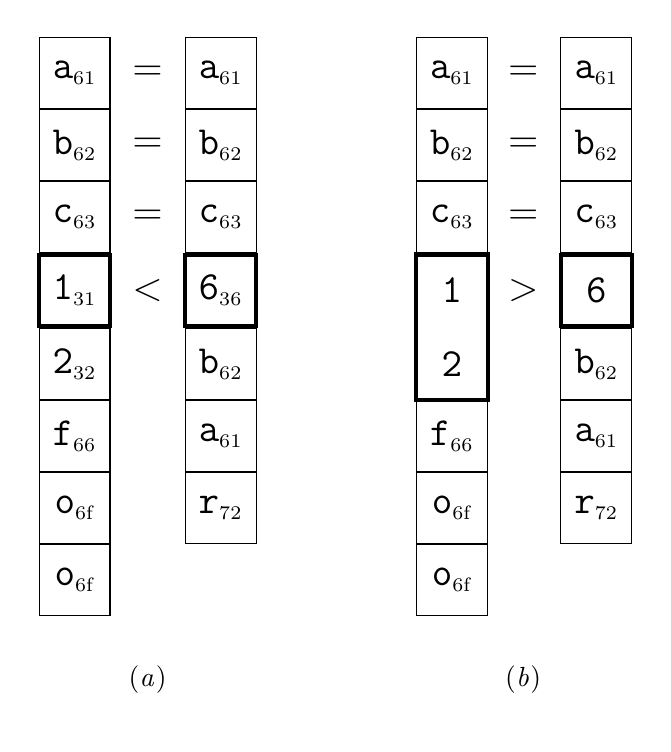
\begin{tikzpicture}[every node/.style={minimum size=9mm},
 ampersand replacement=\&]
\matrix[font={\Large\ttfamily}]
{
  \node[draw]{a\hexsb{61}}; \& \node{$=$}; \& \node[draw]{a\hexsb{61}}; \&[20mm]
  \node[draw]{a\hexsb{61}}; \& \node{$=$}; \& \node[draw]{a\hexsb{61}};
  \\
  \node[draw]{b\hexsb{62}}; \& \node{$=$}; \& \node[draw]{b\hexsb{62}}; \&
  \node[draw]{b\hexsb{62}}; \& \node{$=$}; \& \node[draw]{b\hexsb{62}};
  \\
  \node[draw]{c\hexsb{63}}; \& \node{$=$}; \& \node[draw]{c\hexsb{63}}; \&
  \node[draw]{c\hexsb{63}}; \& \node{$=$}; \& \node[draw]{c\hexsb{63}};
  \\
  \node[draw,ultra thick]{1\hexsb{31}}; \& \node{$<$}; \&
  \node[draw,ultra thick]{6\hexsb{36}}; \&
  \node (n1) {1}; \& \node{$>$}; \& \node[draw,ultra thick]{6};
  \\
  \node[draw]{2\hexsb{32}}; \&  \& \node[draw]{b\hexsb{62}}; \&
  \node (n2) {2}; \&  \& \node[draw]{b\hexsb{62}};
  \\
  \node[draw]{f\hexsb{66}}; \&  \& \node[draw]{a\hexsb{61}}; \&
  \node[draw]{f\hexsb{66}}; \&  \& \node[draw]{a\hexsb{61}};
  \\
  \node[draw]{o\hexsb{6f}}; \&  \& \node[draw]{r\hexsb{72}}; \&
  \node[draw]{o\hexsb{6f}}; \&  \& \node[draw]{r\hexsb{72}};
  \\
  \node[draw]{o\hexsb{6f}}; \&  \& \&
  \node[draw]{o\hexsb{6f}}; \&  \& 
  \\[10pt]
   \& \node[font=\rmfamily]{\subfigfmt{a}};  \& \&
   \& \node[font=\rmfamily]{\subfigfmt{b}};  \& 
  \\
};
\draw[ultra thick] (n1.north east) rectangle (n2.south west);
\end{tikzpicture}%
}
{%
 \caption[Regular letter comparison vs letter-number
 comparison]{Regular letter comparison vs letter-number comparison.
 Comparing the strings \code{abc12foo} and \code{abc6bar}:
 \subfigfmt{a} \optfmt{letter-case}; \subfigfmt{b}
 \optfmt{letternumber-case}.}%
}
{fig:letternumber}
\end{figure}

For example, suppose the first string is \code{abc12foo}
and the second string is \code{abc6bar}.
\Figureref{fig:letternumber}\subfigfmt{a} shows the regular letter
comparison using \csopt[letter-case]{sort}, where the subscript
indicates the hexadecimal character code. The first three characters
from each string are identical (\code{abc}). At this point there's
no difference detected, so the comparator moves on to the next
character, \code{1\hexsb{31}} for the first string and
\code{6\hexsb{36}} for the second string. Since \hex{31} is less than 
\hex{36}, the first string (\code{abc12foo}) is considered less than the second
(\code{abc6bar}).

With the letter-number comparison using
\csopt[letternumber-case]{sort}, the comparator starts in much the
same way. The first three characters from each string are still
identical, so the comparator moves on to the next character,
\code{1} for the first string and \code{6} for the second. 
These are now both recognised as digits, so the comparator
looks ahead and reads in any following digits (if present).  For the
first case, this is the sub-string \code{12} and, for the second
case, \code{6} (\figureref{fig:letternumber}\subfigfmt{b}).  These
are both compared according to their integer representation $12 >
6$, so \code{abc12bar} is considered greater than \code{abc6foo}
(that is, \code{abc12bar} comes after \code{abc6foo}). 

The same result occurs for other numbering systems, for example if
the Basic Latin digits 1, 2 and 6 are replaced with the
corresponding Devanagari digits \devone, \devtwo\ and
\devsix. (But note that the letter comparisons will still be
based on their Unicode values not according to a particular locale.
This type of sort method is intended primarily for symbolic values,
such as chemical formulae, rather than for words or phrases.)

Signed integers are also recognised, so \code{abc-12foo} is less
than \code{abc+6bar}, which is again different from the result
obtained with a straight letter comparator where the
character~\code{+} (\hex{2B})
comes before the character~\code{-} (\hex{2D}). The sign must be followed by at
least one digit for it to be recognised as a number otherwise it's
treated as a punctuation character.

If only one sub-string is numeric
then the \csopt{letter-number-rule} is used to determine the
result. Where both sub-strings are non-numeric, then the 
\csopt{letter-number-punc-rule} setting is used to determine the result
according to the category of the characters, which may be one of the
following:
\begin{itemize}
\item white space: belongs to the Unicode \idx{separatorspace}
category. If both characters are white space, then they are compared
according to their Unicode values otherwise they are ordered according to 
the \csopt{letter-number-punc-rule} setting.

\item letter: belongs to one of the Unicode categories \idx{letteruppercase}, 
\idx{letterlowercase}, \idx{lettertitlecase},
\idx{lettermodifier} or \idx{letterother}. If both characters
are letters then, for sort method \optfmt{letternumber-\meta{modifier}}, 
the characters are compared in the same way as the
corresponding \optfmt{letter-\meta{modifier}} sort method otherwise
they are ordered according to the 
\csopt{letter-number-punc-rule} setting.

\item punctuation: everything else. If both characters are
punctuation, then they are compared according to their Unicode value
otherwise they are ordered according to 
the \csopt{letter-number-punc-rule} setting.
\end{itemize}
For simplicity, the actual sort value used during sorting isn't a
simple string but is converted into a list of objects that represent
one of: letter, integer, space or other (punctuation). This reduces
the amount of parsing of substrings that needs to be performed.

The examples below show the ordering of the list:
\code{CH\textsubscript{2}O}, 
\code{C\textsubscript{10}H\textsubscript{10}O\textsubscript{4}}, 
\code{C\textsubscript{5}H\textsubscript{4}NCOOH}, 
\code{CO}, \code{Cl}, 
\code{Co}, \code{Co\textsubscript{2}O\textsubscript{3}}, 
\code{Co\textsubscript{2}}, \code{CO\textsubscript{2}},
\code{CoMoO\textsubscript{4}} and \code{CoCl\textsubscript{2}},
for the setting
\csopt[between]{letter-number-rule}, where the subscripts are
the Unicode subscript characters.

\begin{itemize}
\item \optfmt{letternumber-case}: case-sensitive
letter-number sort. Example:

\code{CH\textsubscript{2}O}, 
\code{CO},
\code{CO\textsubscript{2}},
\code{C\textsubscript{5}H\textsubscript{4}NCOOH}, 
\code{C\textsubscript{10}H\textsubscript{10}O\textsubscript{4}}, 
\code{Cl}, 
\code{Co}, 
\code{CoCl\textsubscript{2}},
\code{CoMoO\textsubscript{4}}, 
\code{Co\textsubscript{2}},
\code{Co\textsubscript{2}O\textsubscript{3}}.

(Order determined by: $\mathtt{H} < \mathtt{O} < 5 < 10 < \mathtt{l} < \mathtt{o}$.)

\item \optfmt{letternumber-case-reverse}: reverse case-sensitive
letter-number sort. Example:

\code{Co\textsubscript{2}O\textsubscript{3}},
\code{Co\textsubscript{2}},
\code{CoMoO\textsubscript{4}}, 
\code{CoCl\textsubscript{2}},
\code{Co}, 
\code{Cl}, 
\code{C\textsubscript{10}H\textsubscript{10}O\textsubscript{4}}, 
\code{C\textsubscript{5}H\textsubscript{4}NCOOH}, 
\code{CO\textsubscript{2}},
\code{CO},
\code{CH\textsubscript{2}O}.

\item \optfmt{letternumber-nocase}: case-insensitive
letter-number sort. The sort value is first converted to lower
case. Note that \csopt[between]{letter-number-rule} doesn't make
sense in this context as there won't be any \idx!{uppercase} characters in
the sort value, so numbers will always come before letters. Example:

\code{C\textsubscript{5}H\textsubscript{4}NCOOH}, 
\code{C\textsubscript{10}H\textsubscript{10}O\textsubscript{4}}, 
\code{CH\textsubscript{2}O}, 
\code{Cl}, 
\code{CO}, 
\code{Co}, 
\code{CO\textsubscript{2}},
\code{Co\textsubscript{2}},
\code{Co\textsubscript{2}O\textsubscript{3}},
\code{CoCl\textsubscript{2}},
\code{CoMoO\textsubscript{4}}. 

(Order determined by: $5 < 10 < \mathtt{h} < \mathtt{l} < \mathtt{o}$.)

\item \optfmt{letternumber-nocase-reverse}: reverse case-insensitive
letter-number sort, so numbers will now always come after letters. Example:

\code{CoMoO\textsubscript{4}}, 
\code{CoCl\textsubscript{2}},
\code{Co\textsubscript{2}O\textsubscript{3}},
\code{Co\textsubscript{2}},
\code{CO\textsubscript{2}},
\code{Co}, 
\code{CO}, 
\code{Cl}, 
\code{CH\textsubscript{2}O}, 
\code{C\textsubscript{10}H\textsubscript{10}O\textsubscript{4}}, 
\code{C\textsubscript{5}H\textsubscript{4}NCOOH}. 

\item \optfmt{letternumber-upperlower}: upper-lower
letter-number sort. This behaves slightly differently to
\optfmt{letter-upperlower} when used with \csopt[between]{letter-number-rule}
and has a more complicated rule that's determined by the character
following the number and implied numbers inserted between letters. 
(There was a bug in earlier versions that has been corrected in v1.8
so you may find a slightly different ordering when upgrading.)
Example:

\code{CH\textsubscript{2}O}, 
\code{C\textsubscript{5}H\textsubscript{4}NCOOH}, 
\code{C\textsubscript{10}H\textsubscript{10}O\textsubscript{4}}, 
\code{Cl}, 
\code{CO}, 
\code{CO\textsubscript{2}},
\code{Co}, 
\code{Co\textsubscript{2}},
\code{CoCl\textsubscript{2}},
\code{CoMoO\textsubscript{4}}, 
\code{Co\textsubscript{2}O\textsubscript{3}}.

(Order determined by: $\mathtt{H} < 5\mathtt{H} < 10\mathtt{H} <
\mathtt{l} < \mathtt{O} < \mathtt{o}$, and for the terms starting
with \code{CO} or \code{Co}: 2 comes after null and $\mathtt{C} <
\mathtt{M} < 2\mathtt{O}$.)

Compare this with \csopt[before letter]{letter-number-rule} which
results in the order:

\code{C\textsubscript{5}H\textsubscript{4}NCOOH}, 
\code{C\textsubscript{10}H\textsubscript{10}O\textsubscript{4}}, 
\code{CH\textsubscript{2}O}, 
\code{Cl}, 
\code{CO}, 
\code{CO\textsubscript{2}},
\code{Co}, 
\code{Co\textsubscript{2}},
\code{Co\textsubscript{2}O\textsubscript{3}},
\code{CoCl\textsubscript{2}},
\code{CoMoO\textsubscript{4}}.

\item \optfmt{letternumber-upperlower-reverse}: reverse upper-lower
letter-number sort. Example (with  \csopt[between]{letter-number-rule}):

\code{Co\textsubscript{2}O\textsubscript{3}},
\code{CoMoO\textsubscript{4}}, 
\code{CoCl\textsubscript{2}},
\code{Co\textsubscript{2}},
\code{Co}, 
\code{CO\textsubscript{2}},
\code{CO}, 
\code{Cl}, 
\code{C\textsubscript{10}H\textsubscript{10}O\textsubscript{4}}, 
\code{C\textsubscript{5}H\textsubscript{4}NCOOH}, 
\code{CH\textsubscript{2}O}. 

Compare this with \csopt[before letter]{letter-number-rule} which
results in the order:

\code{CoMoO\textsubscript{4}}, 
\code{CoCl\textsubscript{2}},
\code{Co\textsubscript{2}O\textsubscript{3}},
\code{Co\textsubscript{2}},
\code{Co}, 
\code{CO\textsubscript{2}},
\code{CO}, 
\code{Cl}, 
\code{CH\textsubscript{2}O}, 
\code{C\textsubscript{10}H\textsubscript{10}O\textsubscript{4}}, 
\code{C\textsubscript{5}H\textsubscript{4}NCOOH}. 

Remember that the associated settings are reversed
well. So \csopt[before letter]{letter-number-rule} 
results in numbers \emph{after} letters.

\item \optfmt{letternumber-lowerupper}: lower-upper letter-number
sort. As with the upper-lower option, this behaves slightly differently to
\optfmt{letter-lowerupper} when used with \csopt[between]{letter-number-rule}
and has a more complicated rule.
Example:

\code{CH\textsubscript{2}O}, 
\code{C\textsubscript{5}H\textsubscript{4}NCOOH}, 
\code{C\textsubscript{10}H\textsubscript{10}O\textsubscript{4}}, 
\code{Cl}, 
\code{Co}, 
\code{Co\textsubscript{2}},
\code{CoCl\textsubscript{2}},
\code{CoMoO\textsubscript{4}}, 
\code{Co\textsubscript{2}O\textsubscript{3}},
\code{CO}, 
\code{CO\textsubscript{2}}.

Compare this with \csopt[before letter]{letter-number-rule} which
results in the order:

\code{C\textsubscript{5}H\textsubscript{4}NCOOH}, 
\code{C\textsubscript{10}H\textsubscript{10}O\textsubscript{4}}, 
\code{CH\textsubscript{2}O}, 
\code{Cl}, 
\code{Co}, 
\code{Co\textsubscript{2}},
\code{Co\textsubscript{2}O\textsubscript{3}},
\code{CoCl\textsubscript{2}},
\code{CoMoO\textsubscript{4}}, 
\code{CO}, 
\code{CO\textsubscript{2}}.

\item \optfmt{letternumber-lowerupper-reverse}: reverse lower-upper
letter-number sort. Example (with \csopt[between]{letter-number-rule}):

\code{CO\textsubscript{2}},
\code{CO}, 
\code{Co\textsubscript{2}O\textsubscript{3}},
\code{CoMoO\textsubscript{4}}, 
\code{CoCl\textsubscript{2}},
\code{Co\textsubscript{2}},
\code{Co}, 
\code{Cl}, 
\code{C\textsubscript{10}H\textsubscript{10}O\textsubscript{4}}, 
\code{C\textsubscript{5}H\textsubscript{4}NCOOH}, 
\code{CH\textsubscript{2}O}. 

\end{itemize}

\subsubsection{Numerical}
\label{sec:numerical}

The sort methods listed in \tableref{tab:sortoptionsnumerical} 
use numeric comparisons. The sort value is expected to
be a numeric value. If it can't be parsed then it's treated as 0
(and a warning will be written to the transcript).
These all recognise the digits in the Unicode \qt{Number,
Decimal Digit} category but, unlike the hybrid letter-number
comparators above, they don't recognise the superscript or subscript
digits. The \qt{non-locale} in some of the descriptions below
indicates that the method doesn't recognise locale-sensitive
formatting, such as group separators.
\begin{itemize}
\item \optfmt{integer}: integer sort. This is for non-locale integer sort
values.

\item \optfmt{integer-reverse}: as above but reverses the order.

\item \optfmt{hex}: hexadecimal integer sort. This is for non-locale
hexadecimal sort values.

\item \optfmt{hex-reverse}: as above but reverses the order.

\item \optfmt{octal}: octal integer sort. This is for non-locale
octal sort values.

\item \optfmt{octal-reverse}: as above but reverses the order.

\item \optfmt{binary}: binary integer sort. This is for non-locale binary sort
values.

\item \optfmt{binary-reverse}: as above but reverses the order.

\item \optfmt{float}: single-precision sort. This is for non-locale
decimal sort values.

\item \optfmt{float-reverse}: as above but reverses the order.

\item \optfmt{double}: double-precision sort. This is for non-locale
decimal sort values.

\item \optfmt{float-reverse}: as above but reverses the order.

\item \optfmt{numeric}: locale-sensitive numeric sort. Use
\csopt{numeric-locale} to set the locale.

\item \optfmt{numeric-reverse}: as above but reverses the order.

\item \optfmt{currency}: locale-sensitive currency sort. Use
\csopt{numeric-locale} to set the locale.

\item \optfmt{currency-reverse}: as above but reverses the order.

\item \optfmt{percent}: locale-sensitive percent sort. Use
\csopt{numeric-locale} to set the locale.

\item \optfmt{percent-reverse}: as above but reverses the order.

\item \optfmt{numberformat}: locale-sensitive custom numeric sort. Use
\csopt{numeric-locale} to set the locale and
\csopt{numeric-sort-pattern} to set the number pattern.

\item \optfmt{numberformat-reverse}: as above but reverses the order.

\end{itemize}

In general, it doesn't make much sense to have hierarchical entries
that need to be sorted by a number, but it is possible as long as each
level uses the same type of numbering.

\subsubsection{Date-Time}

The sort methods listed in \tableref{tab:sortoptionsdatetime} 
are for dates and times.  Use \csopt{date-sort-format}
and \csopt{date-sort-locale} to specify the date format and locale.
\begin{itemize}
\item \optfmt{date}: sort dates.

\item \optfmt{date-reverse}: as above but reverses the order.

\item \optfmt{datetime}: sort date and time information.

\item \optfmt{datetime-reverse}: as above but reverses the order.

\item \optfmt{time}: sort times.

\item \optfmt{time-reverse}: as above but reverses the order.

\end{itemize}

If the field you want to sort by contains a date then the
simplest way to sort is to ensure the date is in ISO format
and then just use a letter sort. However it may be that
the date is in the format particular to your locale or you have a
mix of \era{AD} and \era{BC}. In which
case you can use one of the date/time sort options (such as
\csopt[date]{sort} or \csopt[date-reverse]{sort}). The locale
is assumed to be your default locale (as given by the \idx{JVM}) 
but if you are using a different locale this can
be set with \csopt{date-sort-locale}. The pattern is assumed
to be the default for that locale but you can change this with
\csopt{date-sort-format}. If you provide your
own custom pattern you must make sure that it matches the selected
\optfmt{sort} option.

Take care if you switch from using the \idx{JRE} to the \idx{CLDR}
 \idx{localeprovider} as you may find the default pattern changes.

The locale and pattern information is used by \bibgls\ to parse the
field.  If the field value can't be parsed then \bibgls\ will issue
a warning and assume the current date (or time).

The actual sort value that's used by the comparator is numeric.  In
the case of the time-based \csopt[datetime]{sort} and
\csopt[time]{sort} (or their \optfmt{-reverse} versions), this value
is the number of milliseconds since 1st~January, 1970. In the case
of \csopt[date]{sort} (or \csopt[date-reverse]{sort}), this value is
obtained from $a(y\times10000 + m\times100 + d)$ where $y$ is the
year, $m$ is the month number, $d$ is the day of month number, and
$a$ is an integer representation of the era ($-1$ for \era{BC} and
$+1$ for \era{AD}).

Unlike the numeric sort methods (such as \csopt[integer]{sort})
the date-time sort methods set the \field{sort} field to a value
that can be more easily parsed within the document and that should
mostly achieve the same ordering if a letter comparator were to be used
with it (except for \era{BC} dates, where the order needs to be
reversed). This has the by-product of providing a field that
you can access within the document that can be more easily parsed by
\LaTeX.

In general, it doesn't make much sense to have hierarchical entries
that need to be sorted by date, but it is possible as long as each
level uses the same date format.

For example, suppose my \ext{bib} file contains:
\begin{codeenv}
\atentry{entry}\marg{journalentry,
  \field{name}=\marg{10 Jan 2017},
  \field{description}=\marg{an interesting journal entry}
}
\end{codeenv}
The \field{name} field uses an abbreviated UK date format.
If all my other entries also use this format in the \field{name}
then I can sort them chronologically:
\begin{codeenv}
\gls{GlsXtrLoadResources}\oarg{
  \csopt[entries]{src},\comment{data in entries.bib}
  \csopt[date]{sort},
  \csopt[en-GB]{date-sort-locale},
  \csopt[medium]{date-sort-format}
}
\end{codeenv}
(The medium format is actually the default for this locale,
and the locale matches my system locale, so I could omit
both \csopt{date-sort-locale} and \csopt{date-sort-format}.)

If \longarg{verbose} mode is on, the transcript will show
the label, sort value and numeric value for each entry.
In this case, the information is:
\begin{verbatim}
journalentry -> '+1 2017-01-10' [20170110]
\end{verbatim}
The first value is the label (\code{journalentry}), the second
value is assigned to the \field{sort} field
(\code{+1 2017-01-10}) and the number in square brackets 
is the actual numeric value used by the comparator. The signed
number at the start of the sort field \code{+1} is the numeric
representation of the era as used for the $a$ variable in the
computation of the numeric value (as described earlier).

If I change the format to \csopt[short]{date-sort-format},
then the date can't be parsed correctly and \bibgls\ will 
issue the following warning:
\begin{verbatim}
Warning: Can't parse sort value '10 Jan 2017' for 'journalentry'
(pattern: 'dd/MM/yyyy')
\end{verbatim}
This shows the value that \bibgls\ is trying to
parse (\code{10 Jan 2017}) for the entry identified by
the given label (\code{journalentry}). The pattern \bibgls\ 
expects is also given (\code{dd/MM/yyyy}).

\optsection{shuffle}

Automatically sets \csopt[random]{sort} and \csopt{flatten}.
The value \meta{seed} may be omitted. If present, it should
be an integer used as a seed for the random number generator.

\optsection{sort-field}

The \csopt{sort-field} key indicates which field provides the sort
value. The \meta{field} must be a recognised field name or you
may use \csopt[id]{sort-field} to sort according to the label.
The default value is the \field{sort} field (which is typically
inferred rather than explicitly set).

Example:
\begin{codeenv}
\gls{GlsXtrLoadResources}\oarg{
 \csopt[entries-terms]{src},\comment{data in entries-terms.bib}
 \csopt[category]{sort-field},\comment{sort by 'category' field}
 \csopt[letter-case]{sort}\comment{case-sensitive letter sort}
}
\end{codeenv}
This sorts the entries according to the \field{category} field using
a case-sensitive letter comparison.

If an entry is missing a value for \meta{field}, then the value of
the fallback field will be used instead. If \csopt{missing-sort-fallback} is
set, then that's used as the fallback, otherwise it depends on the
entry type. 
If no fallback field can be found, the entry's label will be used.

For the specific case with the default \csopt[sort]{sort-field}
setting, the fallback for the \field{sort} field is governed not
only by the entry type but also by some associated settings:

\begin{itemize}
\item For entries types like \atentry{entry} or \atentry{index},
then if the \field{sort} field is missing the value is obtained from
the \field{name} field. If that field is also missing, then the
value is obtained from the particular entry type's fallback for the
\field{name} field. (For example, \field{parent} for
\atentry{entry}.)

\item If the entry is defined with an abbreviation type (for
example, \atentry{abbreviation} or \atentry{acronym}) then if the
\field{sort} field is missing, \bibgls\ will fallback on the field
given by \csopt{abbreviation-sort-fallback}.

\item The symbol-like entry types fallback on the field given by
\csopt{symbol-sort-fallback} if the \field{sort} field is missing.

\item Entries defined using \atentry{bibtexentry} fallback on the field
given by \csopt{bibtexentry-sort-fallback}, which defaults to the
\field{name} field. Note that this only applies to the main entry.
The spawned \atentry{contributor} entries behave like
\atentry{index}.

\end{itemize}
Use \csopt{dual-sort-field} when sorting dual entries.

\optsection{missing-sort-fallback}

With \csopt[\meta{sort-field}]{sort-field}, if the value of the field
identified by \meta{sort-field} is missing, then \bibgls\ behaves as
follows:
\begin{enumerate}
\item If \csopt[\meta{fallback-field}]{missing-sort-fallback} is set, then
\bibgls\ will fallback on the value provided by the field
\meta{fallback-field}.  If \meta{fallback-field} is
missing, then \bibgls\ will query the entry type's fallback for
\meta{fallback-field} (not for \meta{sort-field}).
\item If the entry type has a fallback rule for \meta{sort-field},
then that rule is used. When \csopt[sort]{sort-field} this means:
\begin{itemize}
\item If the entry was defined using
one of the symbol types, then \bibgls\
will fallback on the value given by \csopt{symbol-sort-fallback}.
\item If the entry was defined using
one of the abbreviation types, then \bibgls\
will fallback on the value given by
\csopt{abbreviation-sort-fallback}.
\item If the entry was defined using \atentry{bibtexentry} (but not
the spawned \atentry{contributor} entries), then \bibgls\ will
fallback on the value given by
\csopt{bibtexentry-sort-fallback}.
\end{itemize}
If \meta{sort-field} is not \field{sort}, then there may not be a
fallback, in which case the next condition applies:
\item Otherwise the sort value will be set to the entry label and \bibgls\
will issue a warning.
\end{enumerate}
The default setting is \csopt[\empty]{missing-sort-fallback}, which
means that step~1 above is omitted.

Use \csopt{dual-missing-sort-fallback} when sorting dual entries
separately from primaries, and use
\csopt{secondary-missing-sort-fallback} for \csopt{secondary}
sorting.

\optsection{abbreviation-sort-fallback}

The entry types that define abbreviations (such as
\atentry{abbreviation} and \atentry{acronym}) will, by default,
fallback on the \field{short} field if the \field{sort} field is
missing (assuming \csopt[sort]{sort-field}). If you prefer to
fallback on a different field, then you can use this option to
specify the field. For example,
\csopt[long]{abbreviation-sort-fallback}. Note that if you use
\csopt[name]{sort-field}, then the fallback field will be given by
\csopt{abbreviation-name-fallback} if the \field{name} field is
omitted. The \meta{field} value must be a known field label.

Note that \csopt{missing-sort-fallback} overrides this setting.

\optsection{symbol-sort-fallback}

The entry types that define symbols (such as \atentry{symbol} and
\atentry{number}) will, by default, fallback on the label if the
\field{sort} field is missing (assuming the default
\csopt[sort]{sort-field}). If you prefer to fallback on a different
field, then you can use this option to specify the field. For
example, \csopt[name]{symbol-sort-fallback}.  The \meta{field} value
must be a known field label.

Note that \csopt{missing-sort-fallback} overrides this setting.

\optsection{bibtexentry-sort-fallback}

The main \atentry{bibtexentry} entry types will, by default,
fallback on the \field{name} if the
\field{sort} field is missing (assuming the default
\csopt[sort]{sort-field}). If you prefer to fallback on a different
field, then you can use this option to specify the field.

Note that \csopt{missing-sort-fallback} overrides this setting.

\optsection{trim-sort}

If the interpreter is used to determine the sort value, this setting
governs whether or not the interpreter should trim leading and
trailing spaces. The default setting is \csopt[true]{trim-sort}.

This option automatically sets \csopt[\meta{boolean}]{dual-trim-sort}
and \csopt[\meta{boolean}]{secondary-trim-sort}.

\optsection{sort-replace}

This option may be used to perform regular expression substitutions
on the sort value and has the same syntax as \csopt{labelify-replace}. 
This action is done after the interpreter parses the
sort value (if applicable) and before \csopt{sort-number-pad} (if
applicable). For example, suppose the sort value is:
\begin{codeenv}
\cs{ensuremath}\marg{\ics{approx} 3.14}
\end{codeenv}
then the interpreter will convert this to $\mathtt{\approx}$\texttt{3.14} but:
\begin{codeenv}
\csopt[\marg{\cs{glshex}2248}\marg{}]{sort-replace}
\end{codeenv}
can be used to strip the $\approx$ symbol (\hex{2248}) so that the value can
now be parsed as a number if \csopt[double]{sort} has been used.

Use \csopt{dual-sort-replace} for dual
and \csopt{secondary-sort-replace} for secondary sort methods.

\optsection{sort-rule}

If the \csopt[custom]{sort} option is used, the sort rule must be
provided with \optfmt{sort-rule}. If \csopt{sort} is not set to
\optfmt{custom}, the \optfmt{sort-rule} setting will be ignored.
This setting uses Java's
\href{http://docs.oracle.com/javase/8/docs/api/java/text/RuleBasedCollator.html}{RuleBasedCollator}
class~\cite{rulebasedcollator}, and the rule syntax needs to conform
to that format.

Remember that the options will be expanded as they are written to
the \iext{aux} file, so be careful of any special characters that
occur in the rule. For the special characters \idx{param}
\idx{commentchar} \idx{sbchar} \idx{colsep} \idx{bgroupchar} and
\idx{egroupchar} you can use \ics{cs.hash}, \ics{cs.percent},
\ics{cs.underscore}, \ics{cs.amp}, \ics{cs.openbrace} and
\ics{cs.closebrace}. These will be written to the \ext{aux} file
with the leading backslash, but \bibgls\ will remove it for this
resource option. Remember that the \styfmt{glossaries} package
provides \ics{glsbackslash} and \ics{glstildechar} which can be used
to produce a literal backslash (\idx{backslashchar}) and tilde
(\idx{tildechar}).

You can also
use \stringu\meta{hex} (where \meta{hex} is a hexadecimal
code) to represent a Unicode character. For example:
\begin{codeenv}
\gls{GlsXtrLoadResources}\oarg{
  \csopt[custom]{sort},
  \csopt[< a,A < b,B < c,C < ch,Ch,CH < d,D
   < dd,Dd,DD < e,E < f,F < ff,Ff,FF
   < g,G < ng,Ng,NG < h,H < ij,Ij,IJ
   < i,I < j,J < k,K < l,L < ll,Ll,LL < m,M
   < n,N < o,O < p,P < ph,Ph,PH < q,Q < r,R < rh,Rh,RH
   < s,S < t,T < th,Th,TH < u,U < v,V < w,W < x,X < y,Y < z,Z
   < \stringu00E6,\stringu00C6]{sort-rule}
}
\end{codeenv}
It's best to use \ics{cs.string} rather than \ics{protect} to avoid
unwanted spaces interfering with \meta{hex}. Note that
\sty{glossaries-extra} v1.21+ provides\footnote{The command
definition was moved to \isty{glossaries-extra-bib2gls} from version
1.27 since it's only needed with \bibgls.}\ \ics{glshex}
which just does \stringu\ so you can do
\code{\ics{glshex} 00E6} instead of \code{\stringu00E6}.
This is only one character different, but you can redefine
\ics{glsxtrresourceinit} to locally set \ics{u} to \ics{glshex} while
the protected write is performed. For example:
\begin{codeenv}
\cs{renewcommand}*\marg{\cs{glsxtrresourceinit}}\marg{\cmd{let}\cmd{u}\cs{glshex}}
\end{codeenv}
Then you can just do \code{\csfmt{u}00E6} instead of \code{\stringu00E6}.

The \isty{glossaries-extra-bib2gls} package (which is automatically loaded by
the \styopt{record} option) provides some commands for common rule blocks 
that may be used in the construction of custom rules. For example:
\begin{codeenv}
\csopt[\ics{glsxtrcontrolrules}
 ;\ics{glsxtrspacerules}
 ;\ics{glsxtrnonprintablerules}
 ;\ics{glsxtrcombiningdiacriticrules}
 ,\ics{glsxtrhyphenrules}
 <\ics{glsxtrgeneralpuncrules}
 <\ics{glsxtrdigitrules}
 <\ics{glsxtrfractionrules}
 <\ics{glsxtrMathItalicGreekIrules}
 <\ics{glsxtrGeneralLatinIVrules}
 <\ics{glsxtrLatinAA}
 <\ics{glsxtrLatinOslash}
]{sort-rule}
\end{codeenv}
This places the Greek maths symbols (such as \ics{alpha}) before the
Latin block. See the \sty{glossaries-extra} documentation for
further details of these commands.

You might find it convenient to provide similar commands in a
package for rules you may often need. For example, suppose I have a
package called, say, \styfmt{mapsymbols} for providing map symbols:
\begin{codeenv}
\cmd{NeedsTeXFormat}\marg{LaTeX2e}
\cmd{ProvidesPackage}\marg{mapsymbols}
\comment{some package or font loading stuff here to provide}
\comment{the appropriate symbols}
\cmd{newcommand}\marg{\cmd{Stadium}}\marg{\ldots}
\cmd{newcommand}\marg{\cmd{Battlefield}}\marg{\ldots}
\cmd{newcommand}\marg{\cmd{Harbour}}\marg{\ldots}
\comment{etc}
\strut
\comment{Provide a rule block:}
\cmd{newcommand}\marg{\cmd{MapSymbolOrder}}\marg{\comment{}
 \cs{glshex} 2694 \comment{crossed-swords 0x2694}
 < \cs{glshex} 2693 \comment{anchor 0x2693}
 < \cs{glshex} 26BD \comment{football 0x26BD}
}
\end{codeenv}
In addition to \filefmt{mapsymbols.sty}, I also need to create
\filefmt{mapsymbols.bib} to provide the appropriate definitions for
\bibgls:
\begin{codeenv}
\atentry{preamble}\marg{"\cs{glsxtrprovidecommand}\marg{\cmd{Harbour}}\marg{\ics{char}"2693}
\cs{glsxtrprovidecommand}\marg{\cmd{Battlefield}}\marg{\cs{char}"2694}
\cs{glsxtrprovidecommand}\marg{\cmd{Stadium}}\marg{\cs{char}"26BD}"}
\end{codeenv}
The use of \ics{glsxtrprovidecommand} will override any previous
definitions of these commands in \bibgls's interpreter but will act
like \ics{providecommand} within the document, and so won't
interfere with the commands defined in \filefmt{mapsymbols.sty}.
Now I can just do:
\begin{codeenv}
\cmd{usepackage}\marg{mapsymbols}\comment{my custom package}
\cmd{usepackage}[\styopt{record}]\marg{glossaries-extra}
\strut
\gls{GlsXtrLoadResources}\oarg{
  \csopt[mapsymbols,\comment{<--- my custom mapsymbols.bib}
   entries\comment{data in entries.bib}
  ]{src},
  \csopt[custom]{sort},
  \csopt[\cs{glsxtrcontrolrules}
 ;\cs{glsxtrspacerules}
 ;\cs{glsxtrnonprintablerules}
 ;\cs{glsxtrcombiningdiacriticrules}
 ,\cs{glsxtrhyphenrules}
 <\cs{glsxtrgeneralpuncrules}
 <\cs{glsxtrdigitrules}
 <\cs{glsxtrfractionrules}
 <\cmd{MapSymbolOrder} \comment{<--- custom map symbols}
 <\cs{glsxtrMathItalicGreekIrules}
 <\ics{glsxtrGeneralLatinIrules}
 ]{sort-rule}
}
\end{codeenv}

An alternative to providing \filefmt{mapsymbols.bib} is to provide a
custom package just for \bibgls' use. For example,
\filefmt{mapsymbols-bib2gls.sty}:
\begin{codeenv}
\comment{Provided for \bibgls\ only.}
\comment{Use \cmd{usepackage}\marg{mapsymbols} in the document.}
\cmd{NeedsTeXFormat}\marg{LaTeX2e}
\cmd{ProvidesPackage}\marg{mapsymbols-bib2gls}
\cs{glsxtrprovidecommand}\marg{\cmd{Harbour}}\marg{\ics{char}"2693}
\cs{glsxtrprovidecommand}\marg{\cmd{Battlefield}}\marg{\cs{char}"2694}
\cs{glsxtrprovidecommand}\marg{\cmd{Stadium}}\marg{\cs{char}"26BD}
\cmd{endinput}
\end{codeenv}
and instruct \bibgls\ to parse it with 
\code{\longarg{custom-packages} mapsymbols-bib2gls} (and use
\filefmt{mapsymbols.sty} in the document). Remember that \bibgls\
isn't a \TeX\ engine so make sure to only use simple commands in
this file.

\optsection{break-at}

This option automatically implements
\csopt[\meta{option}]{dual-break-at} and
\csopt[\meta{option}]{secondary-break-at}.

The alphabet sort options (\tableref{tab:sortoptionsrule}) typically
list non-letter characters before alphabetical characters and spaces
are quite often in the ignored set. This means that the alphabet
sort options are naturally in a letter order, similar to
\idx{xindy}['s] \code{ord/letorder} module.  (This isn't the same as
\csopt[letter-nocase]{sort}, which just sorts according to the
Unicode value not according to a particular alphabet.)

In order to replicate \idx{makeindex} and \idx{xindy}['s] default word
order, \bibgls\ splits up the sort value at word boundaries and
inserts a marker (identified by \csopt{break-marker}).
For example, if the sort value is \qt{sea lion} then it's actually
converted to \verb"sea|lion|" whereas \qt{sea} becomes \verb"sea|"
and \qt{seal} becomes \verb"seal|". The default marker is \verb"|"
which is commonly placed in collation rules before digits but 
after the ignored characters, such as spaces and hyphens.

Note that this action removes non-letters, so for example,
if the sort value is \verb"# (parameter)" then it will be converted
to \verb"parameter|" (hash, space and parentheses removed).
If you only want to break at spaces (optionally following a comma)
use the following instead:
\begin{codeenv}
 \csopt[none]{break-at},
 \csopt[\marg{,? +}\marg{|}]{sort-replace}
\end{codeenv}

You can change the construction of the break points with
\csopt[\meta{option}]{break-at} where \meta{option} may be one of:
\begin{itemize}
\item \optfmt{word}: break at word boundaries (default).
Note that what constitutes a word varies
according to the locale but usually anything that's not alphanumeric 
will designate a word-boundary. The characters between words are
discarded.
For example, the sort value \qt{Tom, Dick, and Harry} becomes 
\verb"Tom|Dick|and|Harry", which has discarded the comma and space
characters.
\item \optfmt{character}: break after each character.
\item \optfmt{sentence}: break after each sentence.
\item \optfmt{upper-notlower}: break after any \idx{uppercase} character
that's not followed by a \idx{lowercase} character. For example, 
\qt{MathML} becomes \verb"MathM|L|" and \qt{W3C} becomes
\verb"W|3C|".
\item \optfmt{upper-upper}: break after any \idx{uppercase} character
that's followed by an \idx{uppercase} character.
\item \optfmt{upper-notlower-word}: first applies break-points
according to \optfmt{upper-notlower} and then according to
\optfmt{word}.
\item \optfmt{upper-upper-word}: first applies break-points
according to \optfmt{upper-upper} and then according to
\optfmt{word}.
\item \optfmt{none}: don't create break points. Use this option to
emulate \idx{makeindex} or \idx{xindy}'s letter ordering, or combine
with \csopt{sort-replace} to insert custom break points.
\end{itemize}

This option is ignored when used with the non-alphabetic
\csopt{sort} options. You can find the break points in the
\field{sort} field for the entry's definition in the \ext{glstex}
file (which is provided for information rather than for use in the
document).  Alternatively, use the \longarg{debug} switch to show
the break points in the transcript. (This will also show the
collation rule.) 

\optsection{break-marker}

This option automatically implements the dual and secondary settings
\csopt[\meta{marker}]{dual-break-marker} and
\csopt[\meta{marker}]{secondary-break-marker}.

The break marker can be changed using
\csopt[\meta{marker}]{break-marker}, where \meta{marker} is 
the character to use. For example, \csopt[-]{break-marker} will use a
hyphen. The marker may be empty, which effectively strips the
inter-word punctuation. For example, with
\csopt[\empty]{break-marker}, \qt{Tom, Dick, and Harry} becomes
\code{TomDickandHarry} and \qt{sea lion} simply becomes
\code{sealion}. If \meta{marker} is omitted,
\csopt[\empty]{break-marker} is assumed.

\optsection{sort-number-pad}

This option automatically implements the dual and secondary settings
\csopt[\meta{number}]{dual-sort-number-pad},
\csopt[\meta{number}]{secondary-sort-number-pad}.

If \meta{number} is greater than 1, any integer sub-strings found
in the sort value will be zero-padded up to this value. Since the
\code{-} character is often ignored by rule-based sort methods, 
any signs found will be replaced with the markers given by
\csopt{sort-pad-plus} and \csopt{sort-pad-minus}, which should be
chosen to ensure that negative numbers are ordered before positive
numbers (if this is desired). An unsigned number will have the
\csopt{sort-pad-plus} marker inserted before it. The default value
is \csopt[0]{sort-number-pad}, which doesn't implement any padding.

If you use this with a locale sort method, it's best to also set
\csopt[none]{break-at}, as the default word boundary break points
will likely be confused by a mix of alphanumerics.

\optsection{sort-pad-plus}

This option automatically implements the dual and secondary settings
\csopt[\meta{marker}]{dual-sort-pad-plus},
\csopt[\meta{marker}]{secondary-sort-pad-plus}.

This option only has an effect when used with 
\csopt[\meta{number}]{sort-number-pad} where \meta{number} is
greater than 1. Positive numbers will have their sign replaced with 
\meta{marker}. The default setting is \csopt[>]{sort-pad-plus}.

\optsection{sort-pad-minus}

This option automatically implements the dual and secondary settings
\csopt[\meta{marker}]{dual-sort-pad-minus},
\csopt[\meta{marker}]{secondary-sort-pad-minus}.

This option only has an effect when used with 
\csopt[\meta{number}]{sort-number-pad} where \meta{number} is
greater than 1. Negative numbers will have their sign replaced with 
\meta{marker}. The default setting is \csopt[<]{sort-pad-plus}.

\optsection{identical-sort-action}

This option automatically implements the dual and secondary settings
\csopt[\meta{value}]{dual-identical-sort-action} and
\csopt[\meta{value}]{secondary-identical-sort-action}.

This option determines what the comparator should do if
two entries at the same hierarchical level are considered
equal.  The \meta{value} may be one of:
\begin{itemize}
\item\optfmt{none}: don't take any further action if sort values are
identical;
\item\optfmt{id}: if sort values are identical, compare
the entry labels;
\item\optfmt{original id}: if sort values are identical, compare the
original unprefixed entry labels (as given in the \ext{bib} file);
\item\meta{field}: if sort values are identical, compare
the values from the given \meta{field}.
\end{itemize}
In each case (other than \csopt[none]{identical-sort-action}) a
simple case-sensitive string comparison is used. If \meta{value}
isn't a recognised keyword or valid field an error will occur.  The
default setting is \csopt[id]{identical-sort-action}.  If you're
using one of the sort rules listed in \tableref{tab:sortoptionsrule}
and you also want a locale-sensitive sort used on the fallback, then
you need to use \csopt{sort-suffix} instead.

\bibgls\ allows duplicate sort values, but this can cause a problem
for hierarchical entries where parent entries with duplicate sort
fields are clumped together and their children follow. To prevent
this from happening, the \csopt[id]{identical-sort-action}
setting will fallback on comparing the labels.  Since all labels
must be unique, this means comparisons between two different entries
are all either strictly higher or strictly lower.

This action occurs after any suffixes have been appended through
\csopt{sort-suffix}.

\optsection{sort-suffix}

This option automatically implements the dual and secondary settings
\csopt[\meta{value}]{dual-sort-suffix} and
\csopt[\meta{value}]{secondary-sort-suffix}.
The value may be one of:
\begin{itemize}
\item\optfmt{none}: don't append a suffix to any \field{sort} value;
\item\optfmt{non-unique}: append a numeric suffix to non-unique
  \field{sort} values;
\item\meta{field}: append the value of the given field (if set) to
  the \field{sort} field. The given field must be defined (has an
  associated key for use in \gls{newglossaryentry}) but may be unset.
  If the interpreter is on, the field contents will be interpreted.
  If the field is just a label (such as the \field{category} field)
  you may find it simpler to use
  \csopt[\meta{field}]{identical-sort-action} instead.
\end{itemize}
The default setting is \csopt[none]{sort-suffix}.

This option only affects the alphabetic
(\tableref{tab:sortoptionsrule}), letter
(\tableref{tab:sortoptionsletter}) and letter-number
(\tableref{tab:sortoptionsletternumber}) sort rules.  For the other
types of sort methods (not including the no-sort options listed in
\tableref{tab:sortoptionsnosort}) you'll need to use
\csopt{identical-sort-action} to prevent problems occurring with
duplicate sort values.

In the case of \csopt[non-unique]{sort-suffix}, this will only append a
suffix to the duplicate sort values (within the same hierarchical
level). The first sort value to be encountered isn't given a suffix.

The \csopt[\meta{field}]{sort-suffix} setting will only append a suffix
if that field is set, but (if set) it will apply the suffix to all
\field{sort} values, even those that are unique.

If you use \longarg{verbose}, then \bibgls\ will write information
in the transcript when it appends a suffix to the sort value.  The
message:
\begin{alltt}
Sort value '\meta{sort}' (entry '\meta{id}') not unique for the entry's
hierarchical level.
\end{alltt}
indicates that an entry with the given \meta{sort} value has already
been found within the same hierarchical level as the currently
processed entry (whose label is given by \meta{id}). The same
hierarchical level in this context means that either both entries
don't have a parent or both entries have the same parent. (That is,
the entries are considered siblings.)

This message will then be followed by:
\begin{alltt}
Appending suffix '\meta{suffix}' to the sort value '\meta{sort}' 
for entry '\meta{id}'.
\end{alltt}
which indicates that the entry (identified by the label \meta{id})
has been assigned the sort value given by \meta{sort}\meta{suffix}.
If any break markers are applied, this is done after the suffix has
been appended.

For example, suppose in my document I want to write about \appfmt{makeglossaries}
(the application) and \csfmt{makeglossaries} (the command). I might
decide to define semantic commands:
\begin{codeenv}
\cs{newcommand}*\marg{\cmd{application}}[1]\marg{\ics{texttt}\marg{\idx{param}1}}
\cs{newcommand}*\marg{\cmd{command}}[1]\marg{\cs{texttt}\marg{\cs{glsbackslash} \idx{param}1}}
\end{codeenv}
In my \ext{bib} file I might have:
\begin{codeenv}
\atentry{entry}\marg{cs.makeglossaries,
  \field{name}=\marg{\cmd{command}\marg{makeglossaries}},
  \field{category}=\marg{command},
  \field{description}=\marg{opens glossary files}
}
\strut
\atentry{entry}\marg{ap.makeglossaries,
  \field{name}=\marg{\cmd{application}\marg{makeglossaries}},
  \field{category}=\marg{application},
  \field{description}=\marg{Perl script}
}
\end{codeenv}
If \bibgls\ is provided with the definitions of \csfmt{application}
and \csfmt{command} (by interpreting the \atentry{preamble} or a
package provided with \longarg{custom-packages}) then it will
determine that the sort value for \code{cs.makeglossaries} is
\csfmt{makeglossaries} and the sort value for
\code{ap.makeglossaries} is just \code{makeglossaries}. These are 
two distinct sort values from \bibgls's point of view although the
sort rule may consider them identical if the rule ignores the
\idx{escchar} character (such as the locale sort methods), in which case,
\bibgls\ will then act according to \csopt{identical-sort-action}.

If \bibgls\ isn't provided with these custom definitions, then it
will ignore those semantic commands and both entries will end up with
the sort value \code{makeglossaries}. The second instance will be
recognised as a duplicate and the sort value will be converted to
\code{makeglossaries1} (where the automated suffix is \code{1} and
the suffix marker, see below, is the empty string). Whereas with,
say, \csopt[.]{sort-suffix-marker}\ then the sort value would become
\code{makeglossaries.1}.

For comparison, consider the following document:
\begin{codeenv}
\cmd{documentclass}\marg{article}
\strut
\cmd{usepackage}[\styopt[indexgroup]{style}]\marg{glossaries}
\strut
\ics{cs.makeglossaries}
\strut
\cs{newcommand}*\marg{\cmd{application}}[1]\marg{\cs{texttt}\marg{\idx{param}1}}
\cs{newcommand}*\marg{\cmd{command}}[1]\marg{\cs{texttt}\marg{\cs{glsbackslash} \idx{param}1}}
\strut
\gls{newglossaryentry}\marg{cs.makeglossaries}\marg{\comment{}
  \field{name}=\marg{\cmd{command}\marg{makeglossaries}},
  \field{description}=\marg{opens glossary files}}
\strut
\gls{newglossaryentry}\marg{ap.makeglossaries}\marg{\comment{}
  \field{name}=\marg{\cmd{application}\marg{makeglossaries}},
  \field{description}=\marg{Perl script}}
\strut
\cmd{begin}\marg{document}
\cs{gls}\marg{cs.makeglossaries} and \cs{gls}\marg{ap.makeglossaries}.
\ics{printglossaries}
\cmd{end}\marg{document}
\end{codeenv}

This uses \idx{makeindex}, which puts both entries in the
\qt{Symbols} group (since they both start with \idx{escchar} from the
start of \csfmt{command} and \csfmt{application}, respectively).
The ordering is \appfmt{makeglossaries}, \csfmt{makeglossaries}
because \qt{a} (second character of \csfmt{application}) comes
before \qt{c} (second character of \csfmt{command}).

The switch to \idx{xindy} just involves adding the \styopt{xindy}
package option:
\begin{codeenv}
\cs{usepackage}[\styopt{xindy},\styopt[indexgroup]{style}]\marg{glossaries}
\end{codeenv}
This results in a glossary that only contains one entry,
\csfmt{makeglossaries}, because \idx{xindy} merges entries with
duplicate sort values and the sort values end up as duplicates
because \idx{xindy} discards the \csfmt{application} and
\csfmt{command} control sequences. Although \bibgls\ also ignores
unknown control sequences, it doesn't perform this merger. 

If I add: 
\begin{codeenv}
\atentry{preamble}\marg{"\cs{providecommand}*\marg{\cmd{application}}[1]\marg{\cs{texttt}\marg{\idx{param}1}}
\cs{providecommand}\marg{\cmd{command}}[1]\marg{\cs{texttt}\marg{\cs{glsbackslash} \idx{param}1}}"}
\end{codeenv}
to the earlier \ext{bib} file (called, say, \filefmt{entries.bib})
then the document can be altered to use \bibgls:
\begin{codeenv}
\cmd{documentclass}\marg{article}
\strut
\cmd{usepackage}[\styopt{record},\styopt[indexgroup]{style}]\marg{glossaries-extra}
\strut
\gls{GlsXtrLoadResources}\oarg{\csopt[entries.bib]{src},
  \csopt[non-unique]{sort-suffix},
  \csopt[none]{identical-sort-action}
}
\strut
\cmd{begin}\marg{document}
\cs{gls}\marg{cs.makeglossaries} and \cs{gls}\marg{ap.makeglossaries}.
\cs{printunsrtglossaries}
\cmd{end}\marg{document}
\end{codeenv}
This uses the default \csopt[locale]{sort} which considers \idx{escchar}
an ignored (punctuation) character, so both \csfmt{makeglossaries} and
\appfmt{makeglossaries} are listed in the \qt{M} letter group, even
though the interpreter has determined that the sort value for
\code{cs.makeglossaries} is the literal string \csfmt{makeglossaries}. 
Note that in this case \bibgls\ doesn't detect duplicate sort values
since it only uses a simple string comparison to detect duplicates
rather than using the collator.

If I switch to using a letter-based sort rule instead, for example
\csopt[letter-nocase]{sort}, then \csfmt{makeglossaries} will be
listed in the \qt{Symbols} letter group since the leading \idx{escchar}
from the sort value \csfmt{makeglossaries} isn't ignored with this
rule.

Now let's suppose I use \csopt[false]{interpret-preamble} to prevent 
\bibgls\ from interpreting the preamble:
\begin{codeenv}
\gls{GlsXtrLoadResources}\oarg{\csopt[entries.bib]{src},\csopt[false]{interpret-preamble}}
\end{codeenv}
This means that the custom commands won't be recognised and will
therefore be ignored, so both entries will have their sort values reduced to 
\code{makeglosssaries}.

The first entry to be processed is \code{cs.makeglossaries} because
it's the first to be selected. This is assigned the sort value
\code{makeglossaries}. (Note that, unless you use
\csopt[unsrt]{sort}, the initial selection order is based on the record
order. In this example, \code{cs.makeglossaries} has the first
record in the \ext{aux} file.)

The next entry to be processed is \code{ap.makeglossaries}. This
also ends up with the sort value \code{makeglossaries} so \bibgls\
converts this to \code{makeglossaries1} and (with verbose mode on)
the following messages are written to the transcript:
\begin{verbatim}
Sort value 'makeglossaries' (entry 'ap.makeglossaries') not unique
for the entry's hierarchical level.
Appending suffix '1' to the sort value 'makeglossaries' for entry
'ap.makeglossaries'.
\end{verbatim}
Both entries are listed in the \qt{M} letter group in the order
\csfmt{makeglossaries}, \appfmt{makeglossaries}.

If the records are reversed:
\begin{codeenv}
\cs{gls}\marg{ap.makeglossaries} and \cs{gls}\marg{cs.makeglossaries}.
\end{codeenv}
then the sort value for \code{cs.makeglossaries} is now considered
the duplicate and the order is reversed: \appfmt{makeglossaries},
\csfmt{makeglossaries}.

Suppose now I modify the \ext{bib} file so that
\code{ap.makeglossaries} is defined as:
\begin{codeenv}
\atentry{entry}\marg{ap.makeglossaries,
  \field{name}=\marg{\cmd{application}\marg{makeglossaries}},
  \field{category}=\marg{application},
  \field{description}=\marg{Perl script (must be used with \cs{gls}\marg{cs.makeglossaries})}
}
\end{codeenv}
and suppose the document only contains an explicit reference to
\code{ap.makeglossaries}:
\begin{codeenv}
\cmd{begin}\marg{document}
\cs{gls}\marg{ap.makeglossaries}
\cs{printunsrtglossaries}
\cmd{end}\marg{document}
\end{codeenv}
Now \code{ap.makeglossaries} is the first entry to be selected
because entries with records are always selected before any
(unrecorded) dependencies. In this case \code{cs.makeglossaries} is
only selected because it's required by \code{ap.makeglossaries}. Now
\code{ap.makeglossaries} is the first to have its sort value
assigned, and it's \code{cs.makeglossaries} that has the duplicate.
This means that the ordering in the glossary is now:
\appfmt{makeglossaries}, \csfmt{makeglossaries}.

An oddity occurs if the glossary is moved to the start of the
document:
\begin{codeenv}
\cmd{begin}\marg{document}
\cs{printunsrtglossaries}
\cs{gls}\marg{ap.makeglossaries}
\cmd{end}\marg{document}
\end{codeenv}
In this case, the first document build:
\begin{verbatim}
pdflatex myDoc
bibgls --group --verbose myDoc
pdflatex myDoc
\end{verbatim}
leads to the ordering described above: 
\appfmt{makeglossaries}, \csfmt{makeglossaries}.
However, the next document build has a new record for
\code{cs.makeglossaries} occurring in the glossary (within the
description of \code{ap.makeglossaries}) which means it's now the
first entry to be selected so the ordering switches to:
\csfmt{makeglossaries}, \appfmt{makeglossaries}.
In this type of situation you might be better off with the
\csopt[id]{identical-sort-action} option instead.

Remember that you can temporarily switch off the indexing by locally
setting:
\begin{codeenv*}
\ics{GlsXtrSetDefaultGlsOpts}\marg{\glsopt{noindex}}
\end{codeenv*}
Since the glossary preamble is scoped, you can simply do
\begin{codeenv}
\ics{appto}\ics{glossarypreamble}\marg{\cs{GlsXtrSetDefaultGlsOpts}\marg{\glsopt{noindex}}}
\end{codeenv}
to switch off the indexing within the glossary (or use
\ics{apptoglossarypreamble}). Note that this is
different to using:
\begin{codeenv}
\ics{GlsXtrSetDefaultNumberFormat}\marg{\encap{glsignore}}
\end{codeenv}
which creates an \idx{ignoredrecord}. Even though the record is ignored
(and so won't show in the location list) the record still influences
the selection order and the record count.

\optsection{sort-suffix-marker}

This automatically implements the dual and secondary settings
\csopt[\meta{value}]{dual-sort-suffix-marker} and
\csopt[\meta{value}]{secondary-sort-suffix-marker}.

If a suffix is appended to the sort value (see above) then it will
be separated by the suffix marker, which can be set with
\csopt[\meta{value}]{sort-suffix-marker} where \meta{value} is the
marker. By default the marker is empty. You can use \stringu\meta{hex}
or \cs{glshex}\meta{hex} to indicate Unicode characters outside the
\idx{ASCII} range. If, for some reason, you want to use a special
character, such as \idx{param}, you will need to precede it with
\ics{cs.string} (for example \code{\cs{cs.string}\idx{param}}) or
use the above hexadecimal markup. If you use \ics{cs.hash} it will
be treated as a literal string containing a backslash followed by a
hash character.

\optsection{strength}

This option automatically implements
\csopt[\meta{value}]{dual-strength} and
\csopt[\meta{value}]{secondary-strength}.

The collation strength used by the alphabet sort methods 
(\tableref{tab:sortoptionsrule}) can be set
to the following values: \optfmt{primary} (default),
\optfmt{secondary}, \optfmt{tertiary} or \optfmt{identical}. These
indicate the difference between two characters, but the exact
assignment is locale dependent. See the documentation for Java's
\href{http://docs.oracle.com/javase/8/docs/api/java/text/Collator.html}{\code{Collator}
class}~\cite{collator} for further details.

For example, suppose the file \filefmt{entries.bib} contains:
\begin{codeenv}
\atentry{index}\marg{resume}
\atentry{index}\marg{RESUME}
\atentry{index}\marg{resumee, \field{name}=\marg{r\ics{acute}esum\cs{acute}e}}
\atentry{index}\marg{rat}
\atentry{index}\marg{rot}
\atentry{index}\marg{aardvark}
\atentry{index}\marg{zoo}
\end{codeenv}
and the document contains:
\begin{codeenv}
\cmd{documentclass}\marg{article}
\strut
\cmd{usepackage}[\styopt{record}]\marg{glossaries-extra}
\strut
\gls{GlsXtrLoadResources}\oarg{\csopt[en]{sort},\csopt[entries]{src}}
\strut
\cmd{begin}\marg{document}
\cs{gls}\marg{resumee}, \cs{gls}\marg{resume}, \cs{gls}\marg{RESUME},
\cs{gls}\marg{aardvark}, \cs{gls}\marg{rat}, \cs{gls}\marg{rot}, \cs{gls}\marg{zoo}.
\strut
\cs{printunsrtglossaries}
\cmd{end}\marg{document}
\end{codeenv}
then this uses the default \csopt[primary]{strength}, so the entries
are listed as aardvark, rat, r\'esum\'e, resume, RESUME, rot, zoo.

If the strength is changed to \optfmt{secondary}:
\begin{codeenv}
\gls{GlsXtrLoadResources}\oarg{\csopt[en]{sort},\csopt[entries]{src},\csopt[secondary]{strength}}
\end{codeenv}
then the entries are listed as aardvark, rat, resume, RESUME,
r\'esum\'e, rot, zoo.

If the strength is changed to \optfmt{tertiary} or
\optfmt{identical}, there's no difference from
\csopt[secondary]{strength} for this particular example.

This option is ignored by non-alphabet sorts (such as letter or numeric).

\optsection{decomposition}

This option automatically implements the dual and secondary settings
\csopt[\meta{value}]{dual-decomposition} and
\csopt[\meta{value}]{secondary-decomposition}.

The collation decomposition used by alphabet sort methods
(\tableref{tab:sortoptionsrule}) can be set
to the following values: \optfmt{canonical} (default),
\optfmt{full} or \optfmt{none}. This determines how Unicode composed
characters are handled. The fastest mode is \optfmt{none} but is
only appropriate for languages without accents. The slowest mode is
\optfmt{full} but is the most complete for languages with \idx{non-ASCII}
characters. See the documentation for Java's
\href{http://docs.oracle.com/javase/8/docs/api/java/text/Collator.html}{\code{Collator}
class}~\cite{collator} for further details.
This option is ignored by non-alphabet sorts (such as letter or numeric).

\optsection{letter-number-rule}

This automatically implements the dual and secondary settings
\csopt[\meta{value}]{dual-letter-number-rule}
and
\csopt[\meta{value}]{secondary-letter-number-rule}.

If you use one of the letter-number sort methods
(\tableref{tab:sortoptionsletternumber}), then you can determine the
comparison between a number and letter. The \meta{value} may be
one of:
\begin{itemize}
\item\optfmt{before letter}: numbers are considered less than any
letter.

\item\optfmt{after letter}: numbers are considered greater than any
letter.

\item\optfmt{between}: (default) numbers come between letter cases.
With the \optfmt{letternumber\dhyphen case} sort option, this will put
numbers after \idx{uppercase} and before \idx{lowercase}.  This
setting doesn't make much sense with the
\optfmt{letternumber\dhyphen nocase} option but, if used, this will put
numbers before letters. The \optfmt{letternumber\dhyphen upperlower} and
\optfmt{letternumber\dhyphen lowerupper} options are more complicated. See 
\sectionref{sec:letternumber} for more detail.

\item\optfmt{first}: numbers are considered less than all
characters (including punctuation and spaces).

\item\optfmt{last}: numbers are considered greater than all
characters (including punctuation and spaces).
\end{itemize}
Note that the reverse sort methods will invert this setting.
Remember also that the case-insensitive letter-number sort methods always
first convert the \field{sort} field to \idx{lowercase}, which means that
if you use one of them then there won't be any \idx{uppercase}
characters. 

Use \csopt{letter-number-punc-rule} to determine the relative
position of white space and punctuation.

\optsection{letter-number-punc-rule}

This automatically implements the dual and secondary 
\csopt[\meta{value}]{dual-letter-number-punc-rule}
and
\csopt[\meta{value}]{secondary-letter-number-punc-rule}.

If you use one of the letter-number sort methods
(\tableref{tab:sortoptionsletternumber}), then you can determine the
order of white space and punctuation. In this context, punctuation
means any character that's not considered a letter, a number
or white space. This means that characters such as combining marks
are considered punctuation.

The \meta{value} may be one of the following:
\begin{itemize}
\item\optfmt{punc-space-first}: punctuation comes first, followed by
white space (then letters and optionally numbers according to the letter-number
rule);
\item\optfmt{punc-space-last}: punctuation followed by white space
come last (after letters and optionally numbers according to the letter-number
rule);
\item\optfmt{space-punc-first}: white space comes first, followed by
punctuation (then letters and optionally numbers according to the letter-number
rule);
\item\optfmt{space-punc-last}: white space followed by punctuation
come last (after letters and optionally numbers according to the letter-number
rule); 
\item\optfmt{space-first-punc-last}: white space comes first
(followed by letters and optionally numbers according to the letter-number
rule) and punctuation comes last; 
\item\optfmt{punc-first-space-last}: punctuation comes first
(followed by letters and optionally numbers according to the letter-number
rule) and white space comes last;
\item\optfmt{punc-first-space-zero}: punctuation comes first
(although numbers may come before)
and white space is replaced by the digit~\code{0} (\hex{30});
\item\optfmt{punc-last-space-zero}: punctuation comes last
(although numbers may come after)
and white space is replaced by the digit~\code{0} (\hex{30}).
\item\optfmt{punc-first-space-zero-match-next}: punctuation comes first
(although numbers may come before)
and white space is replaced by the appropriate zero character (see below);
\item\optfmt{punc-last-space-zero-match-next}: punctuation comes last
(although numbers may come after)
and white space is replaced by the appropriate zero character (see below).
\end{itemize}
Remember that the reverse sort methods will invert order governed by this setting.

For the \optfmt{space-zero-match-next} settings, the sort value will
have all spaces replaced with a digit that represents zero. If the
space isn't followed by a digit, the basic Latin \code{0} (\hex{30})
will be used, otherwise \bibgls\ will try to match the zero with the
following digit group. For example, if the space is followed by
\textsuperscript{1} (\hex{B9}) the space will be replaced by
\textsuperscript{0} (\hex{2070}),  resulting in the sub-string
\code{\textsuperscript{01}} (\hex{B9} \hex{2070}). 

If just the \optfmt{space-zero}
(without the \optfmt{-match-next}) is used then the space will just
be replaced with \code{0} resulting in the sub-string
\code{0\textsuperscript{1}} (\hex{30} \hex{2070}). In this case, the
\code{0} will be distinct from \textsuperscript{1} (rather than
being considered a leading zero). However, for 
other numbering systems the \code{0} will be treated as a leading
zero. For example, if the space is followed by the Devanagari digit
one (\hex{0967}) then the sub-string will be \hex{30} \hex{0967} but here the
mixture is allowed to form a number (with a leading zero) as both
characters belong to the Unicode category \idx{numberdecimaldigit}.

This means that the \optfmt{-match-next} settings are only really
needed if the sort string contains the superscript or subscript
digits that don't belong to the \qt{Number, Decimal Digit} category.
The plain \optfmt{space-zero} alternatives are more efficient as
they just perform a simple substitution.

The \TeX\ parser library used by \bibgls\ recognises the standard
\LaTeX\ text-mode commands \ics{textsuperscript}\margm{text} and 
\ics{textsubscript}\margm{text}
and will use the Unicode superscript or subscript characters if they cover every
character in \meta{text}, otherwise HTML markup is used, but that's
then stripped by \bibgls. This means that:
\begin{codeenv}
C\cs{textsubscript}\marg{10}H\cs{textsubscript}\marg{10}O\cs{textsubscript}\marg{4}
\end{codeenv}
will be converted to:
\code{C\textsubscript{10}H\textsubscript{10}O\textsubscript{4}} but:
\begin{codeenv}
X\cs{textsubscript}\marg{1, 2}
\end{codeenv}
will be converted to:
\begin{verbatim}
X<sub>1, 2</sub>
\end{verbatim}
which ends up as \code{X1, 2}.


Note that \csopt[first]{letter-number-rule} and
\csopt[last]{letter-number-rule} overrides this option when
comparing a number with white space or punctuation.

\optsection{numeric-sort-pattern}

If you use the custom \csopt[numberformat]{sort} or
\csopt[numberformat-reverse]{sort}, you need to 
specify the format pattern with this option where
\meta{value} is a pattern recognised by Java's
\href{http://docs.oracle.com/javase/8/docs/api/java/text/DecimalFormat.html}{\code{java.text.DecimalFormat}}
class~\cite{decimalformat}. You can use \stringu\meta{hex} or
\cs{glshex}\meta{hex} to indicate Unicode characters by their
hexadecimal code. You can also use \ics{cs.hash}, \ics{cs.percent},
\ics{cs.underscore}, \ics{cs.amp}, \ics{cs.openbrace} and
\ics{cs.closebrace} to indicate \idx{hashchar}, \idx{percentchar},
\idx{underscorechar}, \idx{ampchar}, \idx{openbracechar} and
\idx{closebracechar}. 

Where the dual or secondary sort uses \optfmt{numberformat}
or \optfmt{numberformat-reverse}, use \csopt{dual-numeric-sort-pattern} for 
\csopt{dual-sort} and \csopt{secondary-numeric-sort-pattern} 
for \csopt{secondary}.

\optsection{numeric-locale}

If you use any of the locale-sensitive numeric sort methods
described in \sectionref{sec:numerical},
such as \csopt[numeric]{sort}, use this option to set
the locale. The value may be:
\begin{itemize}
\item\optfmt{locale}: use Java's default locale (which is usually
the operating system's locale);
\item\optfmt{doc}: use the document's locale or, if not set, assume
\csopt[locale]{numeric-locale};
\item\meta{lang-tag}: set to the locale identified by the given
a valid language tag \meta{lang-tag}.
\end{itemize}
Use \csopt{dual-numeric-locale} for 
\csopt{dual-sort} and \csopt{secondary-numeric-locale} 
for \csopt{secondary}.

\optsection{date-sort-locale}

If you use a date/time sort method (\tableref{tab:sortoptionsdatetime}), 
then you can set the locale used by Java's date-time parser.
The default setting is \csopt[locale]{date-sort-locale}.

The value may be \optfmt{locale} (use Java's default locale),
\optfmt{doc} (use the document's locale) or a valid language tag
\meta{lang-tag} identifying the locale.

Use \csopt{dual-date-sort-locale} and \csopt{secondary-date-sort-locale}
for the dual and secondary.

\optsection{date-sort-format}

If you use a date/time sort method (\tableref{tab:sortoptionsdatetime}), 
then you can set the format used by Java's date-time parser. 
If omitted, \csopt[default]{date-sort-format} is assumed.
The \meta{value} may be one of:
\begin{itemize}
\item\optfmt{default}: use the locale's default format.
\item\optfmt{short}: use the locale's short format.
\item\optfmt{medium}: use the locale's medium format.
\item\optfmt{long}: use the locale's long format.
\item\optfmt{full}: use the locale's full format.
\item\meta{pattern}: provide a custom pattern.
This should match the specifications for Java's
\href{http://docs.oracle.com/javase/8/docs/api/java/text/SimpleDateFormat.html}{\code{SimpleDateFormat}}
class~\cite{simpledateformat}. You may use \stringu\meta{hex} or
\code{\cs{glshex} \meta{hex}} to indicate Unicode characters
or \ics{cs.hash}, \ics{cs.percent}, \ics{cs.underscore}, \ics{cs.amp},
\ics{cs.openbrace} and \ics{cs.closebrace} to indicate
\idx{hashchar}, \idx{percentchar}, \idx{underscorechar},
\idx{ampchar}, \idx{openbracechar} and~\idx{closebracechar}.
\end{itemize}

With the custom setting, if the pattern only contains date (but not
time) information, then it must be used with \csopt[date]{sort}
or \csopt[date-reverse]{sort}. If the pattern only contains time
(but not date) information, then it must be used with
\csopt[time]{sort} or \csopt[time\dhyphen reverse]{sort}. If the pattern
contains date and time information, then it must be used with
\csopt[datetime]{sort} or \csopt[datetime-reverse]{sort}.

For example, suppose each entry provides information about a person
and the \field{user1} field is used to store their date of birth:
\begin{codeenv}
\atentry{entry}\marg{caesar,
  \field{name}=\marg{Gaius Julius Caesar},
  \field{first}=\marg{Julius Caesar},
  \field{text}=\marg{Caesar},
  \field{description}=\marg{Roman politician and general},
  \field{user1}=\marg{13 July 100 BC}
}
\strut
\atentry{entry}\marg{wellington,
  \field{name}=\marg{Arthur Wellesley, 1st Duke of Wellington},
  \field{first}=\marg{Arthur Wellesley (Duke of Wellington)},
  \field{text}=\marg{Wellington},
  \field{description}=\marg{Anglo-Irish soldier and statesman},
  \field{user1}=\marg{1 May 1769 AD}
}
\end{codeenv}
Then the entries can be sorted by date of birth using:
\begin{codeenv}
\gls{GlsXtrLoadResources}\oarg{
  \csopt[entries]{src},\comment{data in entries.bib}
  \csopt[user1]{sort-field},
  \csopt[date]{sort},
  \csopt[d MMM y G]{date-sort-format}
}
\end{codeenv}

The \code{G} (era) date pattern specifier expects a string, such as
\qt{AD}. It will match \idx{lowercase} forms, such as \qt{ad}, so if you
have \code{\cs{textsc}\marg{ad}} the interpreter will convert this to
\code{ad} (stripping the text-block command). However, in general
it's best to supply a semantic command that ensures that the
interpreted result matches the required format.

For example, if \csfmt{era} is provided with:
\begin{codeenv}
\atentry{preamble}\marg{"\cs{providecommand}\marg{\cmd{era}}[1]\marg{\cs{textsc}\marg{\cs{MakeLowercase}\marg{\idx{param}1}}}"}
\end{codeenv}
If the definition is hidden from the interpreter
(\csopt[false]{interpret-preamble}) and the field
value contains \verb|\era{AD}| then the custom command will simply be stripped
leaving \code{AD} which can be matched by \code{G}. 

If the definition is picked up by the interpreter then the field
value will contain \code{ad} (from \ics{MakeLowercase}) but this can
be matched by \code{G}, so it isn't a problem.
However, if the definition of \csfmt{era} is changed so that the era label
supplied in the argument is converted to something that doesn't
match \code{G} then the definition should be hidden from the
interpreter.

Here's a complete document that changes the \field{group} fields to use
the year and era:
\begin{codeenv}
\cmd{documentclass}\marg{article}
\strut
\cmd{usepackage}[\styopt{record},\styopt[indexgroup]{style}]\marg{glossaries-extra}
\strut
\cs{newcommand}\marg{\gls{bibglsdategroup}}[7]\marg{\idx{param}1\idx{param}4\idx{param}7}
\cs{newcommand}\marg{\gls{bibglsdategrouptitle}}[7]\marg{\ics{number}\idx{param}1\cs{cs.space}\idx{param}4}
\strut
\gls{GlsXtrLoadResources}\oarg{
  \csopt[entries]{src},
  \csopt[user1]{sort-field},
  \csopt[date]{sort},
  \csopt[d MMM y G]{date-sort-format},
  \csopt[all]{selection}
}
\strut
\cmd{begin}\marg{document}
\cs{printunsrtglossaries}
\cmd{end}\marg{document}
\end{codeenv}
(The use of \ics{number} strips the leading zero from the year.)

\optsection{group-formation}

If the \field{group} field hasn't been set in
the \ext{bib} file or through options like \csopt{group}, then it is 
assigned according to this option's setting during sorting. Permitted values:
\begin{itemize}
\item\optfmt{default}: the group is assigned according to 
the sort method's default group formation. This is the default
setting.

\item\optfmt{codepoint}: the group is set to
\format{bibglsunicodegroup}, where the first argument is the first
significant character (converted to \idx{lowercase} and decomposed,
if applicable) of the sort value.

\item\optfmt{unicode category}: the group is set to
\format{bibglsunicodegroup}, where the first argument is the label
identifying the Unicode category of the first significant character
of the sort value. For example, the label \code{Ll} signifies a
\idx!{lowercase} letter and \code{Lu} signifies an \idx!{uppercase}
letter.

\item\optfmt{unicode script}: the group is set to
\format{bibglsunicodegroup}, where the first argument is the
label identifying the Unicode script of the first significant
character of the sort value. For example, the label \code{LATIN}
indicates Latin, \code{GREEK} indicates Greek and \code{COMMON}
indicates common characters (such as mathematical Greek characters
that are often used with non-Greek scripts).

\item\optfmt{unicode category and script}: the group is set to
\format{bibglsunicodegroup}, where the first argument is the
label corresponding to the Unicode category and script of the first
significant character of the sort value. For example, the label
\code{Ll.LATIN} indicates a \idx!{lowercase} Latin letter.
\end{itemize}
This option has no effect with \longarg{no-group} or if no sorting
is applied. Use \csopt{secondary-group-formation} for secondary
sorting and \csopt{dual-group-formation} for dual entries.

\section{Secondary Glossary}
\label{sec:secondaryopts}

The secondary glossary may only be used with \csopt[define]{action}
(within the same resource set) since it's incompatible with the copy actions.
You may use \csopt{secondary} in the first resource set and a copy
action in a subsequent resource set.

\optsection{secondary}

It may be that you want to display a glossary twice but with a
different order. For example, the first time alphabetically and the
second time by category.  One way to do this is to have two
\gls{GlsXtrLoadResources} that both load the same \ext{bib} file with
different \csopt{label-prefix} and \csopt{sort} settings, but this
is only possible with \csopt[all]{selection} or by ensuring you
reference each entry with both label prefixes. Another method is
to use \csopt[copy]{action} but this requires a second resource
command with the same selection criteria.

A simpler method is to use a single \gls{GlsXtrLoadResources}
with the \csopt{secondary} option. The value
(which must be supplied) should be in the format:
\begin{definition}
\meta{sort}:\meta{field}:\meta{type}
\end{definition}
or
\begin{definition}
\meta{sort}:\meta{type}
\end{definition}
If the \meta{field} is omitted, the value of \csopt{sort-field} is
used. Remember that when the primary entries are sorted, the
\field{sort} field will be set, which means that the fallback field
(such as \field{name}) won't be used in the secondary sort. In
general it's best to supply the field unless one type is sorted and the
other isn't. (The actual sort value obtained by the secondary sort
will be saved in the \field{secondarysort} field in case you require it.)

The value of \meta{sort} is as for \csopt{sort}, but note
that in this case the sort value \optfmt{unsrt} or \optfmt{none}
means to use the same ordering as the primary entries. For
example, with \csopt[de-CH-1996]{sort},
\csopt[none:copies]{secondary} the \code{copies} list will be
ordered according to \code{de-CH-1996} and not according to the
order in which they were read when the \ext{bib} file or files were
parsed.  If \meta{sort} is \optfmt{custom}, then the rule should be
provided with \csopt{secondary-sort-rule}.

This option will copy all the selected entries into the glossary labelled
\meta{type} sorted according to \meta{sort} (using \meta{field} as
the sort value). Note that this \emph{just copies the entry's label}
to the second glossary list rather than creating a duplicate entry,
which saves resources but it means that all the fields will be
identical. If you want groups in your glossary, the group
information for the secondary glossary will be stored in the
internal \field{secondarygroup} field. The \field{group} field will
contain the group for the primary glossary.

In order to switch fields in \ics{printunsrtglossary}, you need at
least v1.21 of \sty{glossaries-extra} which provides
\ics{glsxtrgroupfield} to keep track of the appropriate field label.
If this command is defined, the preamble for the secondary glossary 
will be adjusted to locally change the field to
\field{secondarygroup}. With older versions, the group information
in the secondary glossary will be the same as for the primary
glossary.

(If the glossary \meta{type} doesn't exist, it will be
defined with \ics{provideignoredglossary*}\margm{type}.)
Note that if the glossary already exists and contains entries,
the existing entries aren't re-ordered. The new entries are
simply appended to the list.

For example, suppose the \ext{bib} file contains entries like:
\begin{codeenv}
\atentry{entry}\marg{quartz,
  \field{name}=\marg{quartz},
  \field{description}=\marg{hard mineral consisting of silica},
  \field{category}=\marg{mineral}
}
\strut
\atentry{entry}\marg{cabbage,
  \field{name}=\marg{cabbage},
  \field{description}=\marg{vegetable with thick green or purple leaves},
  \field{category}=\marg{vegetable}
}
\strut
\atentry{entry}\marg{waterfowl,
  \field{name}=\marg{waterfowl},
  \field{description}=\marg{any bird that lives in or about water},
  \field{category}=\marg{animal}
}
\end{codeenv}
and the document preamble contains:
\begin{codeenv}
\gls{GlsXtrLoadResources}\oarg{\csopt[entries]{src},\csopt[en-GB]{sort},
  \csopt[en-GB:category:topic]{secondary}
}
\end{codeenv}
This sorts the primary entries according to the default
\csopt{sort-field} and then sorts the entries according
to the \field{category} field and copies this list to
the \code{topic} glossary (which will be provided if not defined.)

The secondary list can be displayed with the hypertargets switched
off to prevent duplicates. The cross-references will link to the
original glossary.

For example:
\begin{codeenv*}
\ics{printunsrtglossary}\oarg{\printglossopt[Summary (alphabetical)]{title}}
\ics{printunsrtglossary}\oarg{\printglossopt[Summary (by topic)]{title},\printglossopt[false]{target}}
\end{codeenv*}

The alternative (or if more than two lists are required) is to
reload the same \ext{bib} file with different label prefixes.
For example, if the entries are stored in \filefmt{entries.bib}:
\begin{codeenv}
\cs{newglossary*}\marg{nosort}\marg{Symbols (Unsorted)}
\cs{newglossary*}\marg{byname}\marg{Symbols (Letter Order)}
\cs{newglossary*}\marg{bydesc}\marg{Symbols (Ordered by Description)}
\cs{newglossary*}\marg{byid}\marg{Symbols (Ordered by Label)}
\strut
\gls{GlsXtrLoadResources}\oarg{
  \csopt[entries]{src},\comment{entries.bib}
  \csopt[unsrt]{sort},
  \csopt[nosort]{type}
}
\strut
\gls{GlsXtrLoadResources}\oarg{
  \csopt[entries]{src},\comment{entries.bib}
  \csopt[letter-case]{sort},
  \csopt[byname]{type},
  \csopt[byname.]{label-prefix}
}
\strut
\gls{GlsXtrLoadResources}\oarg{
  \csopt[entries]{src},\comment{entries.bib}
  \csopt[locale]{sort},
  \csopt[description]{sort-field},
  \csopt[bydesc]{type},
  \csopt[bydesc.]{label-prefix}
}
\strut
\gls{GlsXtrLoadResources}\oarg{
  \csopt[entries]{src},\comment{entries.bib}
  \csopt[letter]{sort},
  \csopt[id]{sort-field},
  \csopt[byid]{type},
  \csopt[byid.]{label-prefix}
}
\end{codeenv}

\optsection{secondary-missing-sort-fallback}

As \csopt{missing-sort-fallback} but for secondary sorting.

\optsection{secondary-trim-sort}

As \csopt{trim-sort} but for secondary sorting.

\optsection{secondary-sort-replace}

As \csopt{sort-replace} but for secondary sorting.

\optsection{secondary-sort-rule}

As \csopt{sort-rule} but for secondary custom sorting.

\optsection{secondary-break-at}

As \csopt{break-at} but for secondary entries.

\optsection{secondary-break-marker}

As \csopt{break-marker} but for secondary entries.

\optsection{secondary-sort-number-pad}

As \csopt{sort-number-pad} but for secondary entries.

\optsection{secondary-sort-pad-plus}

As \csopt{sort-pad-plus} but for secondary entries.

\optsection{secondary-sort-pad-minus}

As \csopt{sort-pad-minus} but for secondary entries.

\optsection{secondary-identical-sort-action}

As \csopt{identical-sort-action} but for secondary entries.

\optsection{secondary-sort-suffix}

As \csopt{sort-suffix} but for secondary entries.

\optsection{secondary-sort-suffix-marker}

As \csopt{sort-suffix-marker} but for secondary entries.

\optsection{secondary-strength}

As \csopt{strength} but for secondary entries.

\optsection{secondary-decomposition}

As \csopt{decomposition} but for secondary entries.

\optsection{secondary-letter-number-rule}

As \csopt{letter-number-rule} but for secondary letter-number sorting.

\optsection{secondary-letter-number-punc-rule}

As \csopt{letter-number-punc-rule} but for secondary letter-number sorting.

\optsection{secondary-numeric-sort-pattern}

As \csopt{numeric-sort-pattern} but for secondary
locale-sensitive numeric sorting.

\optsection{secondary-numeric-locale}

As \csopt{numeric-locale} but for secondary
locale-sensitive numeric sorting.

\optsection{secondary-date-sort-locale}

As \csopt{date-sort-locale} but for secondary date-time sorting.

\optsection{secondary-date-sort-format}

As \csopt{date-sort-format} but for secondary date-time sorting.

\optsection{secondary-group-formation}

As \csopt{group-formation} but for secondary sorting.

\section{Dual Entries}
\label{sec:dualopts}

\subsection{General Dual Settings}
\label{sec:dualoptsgeneral}

\optsection[\subsubsection]{dual-prefix}

This option indicates the prefix to use for the dual entries. The
default value is \idprefix{dual} (including the terminating period). 
Any references to dual entries within the \ext{bib} file should use
the prefix \idprefix{dual} which will be replaced by \meta{value}
when the \ext{bib} file is parsed.

As from version 1.8, the dual label prefix is identified
in the \ext{glstex} file with:
\begin{codeenv}
\format{bibglsdualprefixlabel}
\end{codeenv}

\optsection[\subsubsection]{primary-dual-dependency}

This is a boolean setting that determines whether or not primary and
dual entries should be considered mutual dependencies. The default value is
\csopt[true]{primary-dual-dependency}, which means that if a primary
has records then the dual is added as a dependency and vice versa.
The setting \csopt[false]{primary-dual-dependency} can't be used
with \csopt[none]{dual-sort} or \csopt[use]{dual-sort} (but may be
used with \csopt[combine]{dual-sort} and \csopt[none]{sort} or
\csopt[use]{sort}).

\optsection[\subsubsection]{combine-dual-locations}

This setting allows the location lists for each primary entry
to be merged with that of the corresponding dual entry.
The \meta{value} may be one of:
\begin{itemize}
\item\optfmt{false} This is the default setting. The location lists
aren't combined.
\item\optfmt{both} Both the primary and dual are given the combined
location list.
\item\optfmt{dual} Only the dual is given the combined location
list. The primary's location list is emptied.
\item\optfmt{primary} Only the primary is given the combined
location list. The dual's location list is emptied.
\end{itemize}

For example, suppose the file \filefmt{entries.bib} contains:
\begin{codeenv}
\atentry{dualindexentry}\marg{array,
  \field{description}=\marg{ordered list of values}
}
\strut
\atentry{dualindexentry}\marg{vector,
  \field{name}=\marg{vector},
  \field{description}=\marg{column or row of values}
}
\strut
\atentry{dualindexentry}\marg{set,
  \field{description}=\marg{collection of values}
}
\strut
\atentry{dualindexentry}\marg{matrix,
  \field{plural}=\marg{matrices},
  \field{description}=\marg{rectangular array of values}
}
\end{codeenv}
and the document contains:
\begin{codeenv}
\cmd{documentclass}\marg{article}
\strut
\cmd{usepackage}[colorlinks]\marg{hyperref}
\cmd{usepackage}[\styopt{record},\styopt{index},\styopt[indexgroup]{style}]\marg{glossaries-extra}
\strut
\gls{GlsXtrLoadResources}\oarg{
 \csopt[entries]{src},
 \csopt[index]{type},
 \csopt[idx.]{label-prefix},
 \csopt[gls.]{dual-prefix},
 \csopt[main]{dual-type}
}
\strut
\cmd{begin}\marg{document}
\cs{gls}\marg{gls.array}, \cs{gls}\marg{gls.vector}, \cs{gls}\marg{gls.set}, \cs{gls}\marg{gls.matrix}.
\strut
\cmd{newpage}
\cs{gls}\marg{gls.array}, \cs{gls}\marg{idx.vector}, \cs{gls}\marg{idx.set}, \cs{gls}\marg{gls.matrix}.
\strut
\cmd{newpage}
\cs{gls}\marg{gls.array}, \cs{gls}\marg{gls.vector}, \cs{gls}\marg{gls.set}, \cs{gls}\marg{gls.matrix}.
\strut
\cs{printunsrtglossaries}
\cmd{end}\marg{document}
\end{codeenv}
In this case, the primary entries are placed in the \code{index}
glossary type and are assigned the prefix \idprefixfmt{idx} but only
two of the primary entries have been used in the document (both on
page~2).

The dual entries are assigned the prefix \idprefixfmt{gls} and are
placed in the \code{main} glossary. The \code{gls.array} 
and \code{gls.matrix} entries have been indexed on pages~1, 2 and~3.
The \code{gls.vector} and \code{gls.set} entries have been indexed
on pages~1 and~3.

With the default setting, some of the locations are in the
\code{main} glossary (corresponding to \code{\cs{gls}\marg{gls.array}},
\code{\cs{gls}\marg{gls.vector}}, \code{\cs{gls}\marg{gls.set}} and
\code{\cs{gls}\marg{gls.matrix}}) and some of the locations are in the
\code{index} glossary (corresponding to \code{\cs{gls}\marg{idx.vector}}
and \code{\cs{gls}\marg{idx.set}}).

If the option \csopt[primary]{combine-dual-locations} is added to
the resource set, then all the locations are moved to the
\code{index} glossary. The entries in the \code{main} glossary no
longer have locations. This is actually preferable for this type
of document and it's best not to reference the primary (index)
entries as the hyperlink created by \ics{gls} will point to the
index, but these entries don't have descriptions, so it's less
useful than referencing the dual (main) entries as then the
hyperlink can point to the definition in the \code{main} glossary.


\subsection{Dual Fields}
\label{sec:dualoptsfields}

\optsection[\subsubsection]{dual-type}

This option sets the \field{type} field for all dual
entries. (The primary entries obey the \csopt{type} option.) This
will override any value of \field{type} provided in the \ext{bib}
file (or created through a mapping). The \meta{value} is required and
should be one of:
\begin{itemize}
\item \optfmt{same as entry}: sets the \field{type} to the entry
type (\idx!{lowercase} and without 
the initial \code{@}). For example, if the entry was defined with
\atentry{dualentry}, the \field{type} will be set to
\optfmt{dualentry}.
If you've used \csopt{entry-type-aliases}, this refers to the target
entry type not the original entry type provided in the \ext{bib}
file.

\item \optfmt{same as original entry}: set the \field{type} field
to the original entry type (\idx!{lowercase} and without 
the initial \code{@}) before it was aliased (behaves like 
\optfmt{same as entry} if the entry type wasn't aliased).

\item \optfmt{same as base}: sets the \field{type} to the base name
of the \ext{bib} file (without the extension) that provided the
entry definition (new to v1.1);

\item \optfmt{same as primary}: sets the \field{type} to the same as
the corresponding primary entry's \field{type} (which may have been
set with \csopt{type}). If the primary entry doesn't have the
\field{type} field set, the dual's \field{type} will remain
unchanged.

\item \meta{label}: sets the \field{type} field to \meta{label}.
\end{itemize}

Remember that the glossary with that label must have already 
been defined (see \sectionref{sec:newglossary}).
For example:
\begin{codeenv}
\cs{newglossary*}\marg{english}\marg{English}
\cs{newglossary*}\marg{french}\marg{French}
\strut
\gls{GlsXtrLoadResources}\oarg{\csopt[entries]{src},\csopt[en]{sort},\csopt[fr]{dual-sort},
 \csopt[english]{type},
 \csopt[french]{dual-type}}
\end{codeenv}
Alternatively:
\begin{codeenv}
\cs{newglossary*}\marg{dictionary}\marg{Dictionary}
\strut
\gls{GlsXtrLoadResources}\oarg{\csopt[entries]{src},\csopt[en]{sort},\csopt[fr]{dual-sort},
 \csopt[dictionary]{type},
 \csopt[same as primary]{dual-type}}
\end{codeenv}

\optsection[\subsubsection]{dual-category}

This option sets the \field{category} field for all dual
entries. (The primary entries obey the \csopt{category} option.) This
will override any value of \field{category} provided in the \ext{bib}
file (or created through a mapping). The \meta{value} may be empty or
one of:
\begin{itemize}
\item \optfmt{same as entry}: sets the \field{category} to the entry
type (\idx{lowercase} and without 
the initial \code{@}). For example, if the entry was defined with
\atentry{dualentry}, the \field{category} will be set to
\optfmt{dualentry}.
If you've used \csopt{entry-type-aliases}, this refers to the target
entry type not the original entry type provided in the \ext{bib}
file.

\item \optfmt{same as original entry}: set the \field{category} field
to the original entry type (\idx{lowercase} and without 
the initial \code{@}) before it was aliased (behaves like 
\optfmt{same as entry} if the entry type wasn't aliased).

\item \optfmt{same as base}: sets the \field{category} to the base
name of the \ext{bib} file (without the extension) that provided the
entry definition (new to v1.1);

\item \optfmt{same as primary}: sets the \field{category} to the
same as the corresponding primary entry's \field{category} (which
may have been set with \csopt{category}). If the primary entry
doesn't have the \field{category} field set, the dual's
\field{category} will remain unchanged.

\item \optfmt{same as type}: sets the \field{category} to the same
as the value of the entry's \field{type} field (which may have been
set with \csopt{dual-type}). If the entry doesn't have the
\field{type} field set, the \field{category} will remain unchanged.

\item \meta{label}: sets the \field{category} field to \meta{label}.
\end{itemize}

\optsection[\subsubsection]{dual-counter}

As \csopt{counter} but for the dual entries. In this case
\meta{value} may be the name of the counter or 
\optfmt{same as primary} which uses the counter for the primary
entry.

\optsection[\subsubsection]{dual-short-case-change}

As \csopt{short-case-change} but applies to the \field{dualshort}
field instead.

\optsection[\subsubsection]{dual-long-case-change}

As \csopt{long-case-change} but applies to the \field{duallong}
field instead.

\optsection[\subsubsection]{dual-field}

If this option is used, this will add \ics{glsxtrprovidestoragekey}
to the start of the \iext{glstex} file providing the key given by
\meta{value}.  Any entries defined using a dual entry type, such as
\atentry{dualentry}, will be written to the \ext{glstex} file with
an extra field called \meta{value} that is set to the mirror entry.
If \meta{value} is omitted \csopt[dual]{dual-field} is assumed. If
you use a different value, you will need to redefine
\gls{GlsXtrDualField} (either locally or globally).

For example, if the \ext{bib} file contains:
\begin{codeenv}
\atentry{dualentry}\marg{child,
  \field{name}=\marg{child},
  \field{plural}=\marg{children},
  \field{description}=\marg{enfant}
}
\end{codeenv}
Then with \csopt[dual]{dual-field} (or simply \csopt{dual-field}
without a value) this will first add the line:
\begin{codeenv}
\cs{glsxtrprovidestoragekey}\marg{\field{dual}}\marg{}\marg{}
\end{codeenv}
at the start of the file and will include the line:
\begin{codeenv*}
\field{dual}=\marg{dual.child},
\end{codeenv*}
for the primary entry (\code{child}) and the line:
\begin{codeenv}
\field{dual}=\marg{child},
\end{codeenv}
for the dual entry (\code{dual.child}). It's then possible to
reference one entry from the other. For example, the post-description 
hook could contain:
\begin{codeenv}
 \cs{ifglshasfield}\marg{\field{dual}}\marg{\cs{glscurrententrylabel}}
 \marg{\comment{}
   \cs{space}
   (\cs{glshyperlink}\marg{\cs{glscurrentfieldvalue}})\comment{}
 }\comment{}
 \marg{}\comment{}
\end{codeenv}
Note that this new field won't be available for use within the
\iext{bib} file (unless it was previously defined in the document
before \gls!{glsxtrresourcefile}).

\optsection[\subsubsection]{dual-date-time-field-format}

As \csopt{date-time-field-format} but is used for dual entries.

\optsection[\subsubsection]{dual-date-field-format}

As \csopt{date-field-format} but is used for dual entries.

\optsection[\subsubsection]{dual-time-field-format}

As \csopt{time-field-format} but is used for dual entries.

\optsection[\subsubsection]{dual-date-time-field-locale}

As \csopt{date-time-field-locale} but is used for dual entries.

\optsection[\subsubsection]{dual-date-field-locale}

As \csopt{date-field-locale} but is used for dual entries.

\optsection[\subsubsection]{dual-time-field-locale}

As \csopt{time-field-locale} but is used for dual entries.

\subsection{Dual Sorting}
\label{sec:dualoptssort}

\optsection[\subsubsection]{dual-sort}

This option indicates how to sort the dual entries. The primary
entries are sorted with the normal entries according to
\csopt{sort}, and the dual entries are sorted according to
\csopt{dual-sort} unless \csopt[combine]{dual-sort} in which case the dual
entries will be combined with the primary entries and all the
entries will sorted together according to the \csopt{sort} option.

If \meta{value} isn't set to \optfmt{combine} then the dual
entries are sorted separately according to \meta{value} (as per
\csopt{sort}) and the dual entries will be appended at the end of
the \iext{glstex} file. The field used by the comparator is given by
\csopt{dual-sort-field}.
If \csopt[custom]{dual-sort}, then the dual entries are sorted according to the 
rule provided by \csopt{dual-sort-rule}.

For example:
\begin{codeenv}
\gls{GlsXtrLoadResources}\oarg{
 \csopt[entries-dual]{src},
 \csopt[en]{sort},
 \csopt[de-CH-1996]{dual-sort}
}
\end{codeenv}
This will sort the primary entries according to \optfmt{en}
(English) and the secondary entries according to \optfmt{de-CH-1996} 
(Swiss German new orthography) whereas:
\begin{codeenv}
\gls{GlsXtrLoadResources}\oarg{
 \csopt[entries-dual]{src},
 \csopt[en-GB]{sort},
 \csopt[combine]{dual-sort}
}
\end{codeenv}
will combine the dual entries with the primary entries and sort them
all according to the \optfmt{en-GB} locale (British English).

If not set, \csopt{dual-sort} defaults to \optfmt{combine}. If
\meta{value} is omitted, \optfmt{locale} is assumed.

\optsection[\subsubsection]{dual-sort-field}

This option indicates the field to use when sorting dual entries
(when they haven't been combined with the primary entries). The
default value is the same as the \csopt{sort-field} value.

\optsection[\subsubsection]{dual-missing-sort-fallback}

As \csopt{missing-sort-fallback} but for dual sorting.

\optsection[\subsubsection]{dual-trim-sort}

As \csopt{trim-sort} but for dual sorting.

\optsection[\subsubsection]{dual-sort-replace}

As \csopt{sort-replace} but for dual sorting.

\optsection[\subsubsection]{dual-sort-rule}

As \csopt{sort-rule} but for \csopt[custom]{dual-sort}.

\optsection[\subsubsection]{dual-break-at}

As \csopt{break-at} but for dual entries.

\optsection[\subsubsection]{dual-break-marker}

As \csopt{break-marker} but for dual entries.

\optsection[\subsubsection]{dual-sort-number-pad}

As \csopt{sort-number-pad} but for dual entries.

\optsection[\subsubsection]{dual-sort-pad-plus}

As \csopt{sort-pad-plus} but for dual entries.

\optsection[\subsubsection]{dual-sort-pad-minus}

As \csopt{sort-pad-minus} but for dual entries.

\optsection[\subsubsection]{dual-identical-sort-action}

As \csopt{identical-sort-action} but for dual entries.

\optsection[\subsubsection]{dual-sort-suffix}

As \csopt{sort-suffix} but for dual entries.

\optsection[\subsubsection]{dual-sort-suffix-marker}

As \csopt{sort-suffix-marker} but for dual entries.

\optsection[\subsubsection]{dual-strength}

As \csopt{strength} but for dual entries.

\optsection[\subsubsection]{dual-decomposition}

As \csopt{decomposition} but for dual entries.

\optsection[\subsubsection]{dual-letter-number-rule}

As \csopt{letter-number-rule} but for dual entries that use a
letter-number sort.

\optsection[\subsubsection]{dual-letter-number-punc-rule}

As \csopt{letter-number-punc-rule} but for dual entries that use a
letter-number sort.

\optsection[\subsubsection]{dual-numeric-sort-pattern}

As \csopt{numeric-sort-pattern} but for dual entries that use a
locale-sensitive numeric sort.

\optsection[\subsubsection]{dual-numeric-locale}

As \csopt{numeric-locale} but for dual entries that use a
locale-sensitive numeric sort.

\optsection[\subsubsection]{dual-date-sort-locale}

As \csopt{date-sort-locale} but for dual entries that
use a date/time sort.

\optsection[\subsubsection]{dual-date-sort-format}

As \csopt{date-sort-format} but for dual entries that
use a date/time sort.

\optsection[\subsubsection]{dual-group-formation}

As \csopt{group-formation} but for dual sorting.


\subsection{Dual Mappings}
\label{sec:dualoptsmap}

\optsection[\subsubsection]{dual-entry-map}

This setting governs the behaviour of \atentry{dualentry}
definitions. The value consists of two comma-separated lists of
equal length identifying the field mapping used to create the dual
entry from the primary one. Note that the \field{alias} field
can't be mapped.

The default setting is:
\begin{codeenv}
\csopt[
  \marg{\field{name},\field{plural},\field{description},\field{descriptionplural}},
  \marg{\field{description},\field{descriptionplural},\field{name},\field{plural}}
]{dual-entry-map}
\end{codeenv}
The dual entry is created by copying the value of the field in the
first list \meta{list1} to the field in the corresponding place in the second
list \meta{list2}. Any additional fields are copied over to the same
field.
For example:
\begin{codeenv}
\atentry{dualentry}\marg{cat,
  \field{name}=\marg{cat},
  \field{description}=\marg{chat},
  \field{see}=\marg{dog}
}
\end{codeenv}
defines two entries. The primary entry is essentially like:
\begin{codeenv}
\atentry{entry}\marg{cat,
  \field{name}=\marg{cat},
  \field{plural}=\marg{cat\cs{glspluralsuffix} },
  \field{description}=\marg{chat},
  \field{descriptionplural}=\marg{chat\cs{glspluralsuffix} },
  \field{see}=\marg{dog}
}
\end{codeenv}
and the dual entry is essentially like:
\begin{codeenv}
\atentry{entry}\marg{dual.cat,
  \field{description}=\marg{cat},
  \field{descriptionplural}=\marg{cat\cs{glspluralsuffix} },
  \field{name}=\marg{chat},
  \field{plural}=\marg{chat\cs{glspluralsuffix} },
  \field{see}=\marg{dog}
}
\end{codeenv}
(except they're defined using \gls{bibglsnewdualentry} instead of
\gls{bibglsnewentry}, and each is considered dependent on the other.)

The \field{see} field isn't listed in \csopt{dual-entry-map} so its
value is simply copied directly over to the \field{see} field in the
dual entry. Note that the missing \field{plural} and
\field{descriptionplural} fields have been filled in using their
fallback values.

In general \bibgls\ doesn't try to supply missing fields, but in the
dual entry cases it needs to do this for the mapped fields. This is
because the shuffled fields might have different default values from
the \styfmt{glossaries-extra} package's point of view. For example, 
\gls{longnewglossaryentry} doesn't provide a default for
\field{descriptionplural} if it hasn't been set.

\optsection[\subsubsection]{dual-abbrv-map}

This is like \csopt{dual-entry-map} but applies to
\atentry{dualabbreviation} rather than \atentry{dualentry}. 
Note that the \field{alias} field can't be mapped. The
default setting is:
\begin{codeenv}
\csopt[
  \marg{\field{short},\field{shortplural},\field{long},\field{longplural},\field{dualshort},\field{dualshortplural},
   \field{duallong},\field{duallongplural}},
  \marg{\field{dualshort},\field{dualshortplural},\field{duallong},\field{duallongplural},\field{short},\field{shortplural},
   \field{long},\field{longplural}}
]{dual-abbrv-map}
\end{codeenv}

This essentially flips the \field{short} field with the
\field{dualshort} field and the \field{long} field with the
\field{duallong} field. See \atentry{dualabbreviation}
for further details.

\optsection[\subsubsection]{dual-abbrventry-map}

This is like \csopt{dual-entry-map} but applies to
\atentry{dualabbreviationentry} rather than \atentry{dualentry}. 
Note that the \field{alias} field can't be mapped. The
default setting is:
\begin{codeenv}
\csopt[
  \marg{\field{long},\field{short},\field{shortplural}},
  \marg{\field{name},\field{text},\field{plural}}
]{dual-abbrventry-map}
\end{codeenv}
See \atentry{dualabbreviationentry} for further details.


\optsection[\subsubsection]{dual-symbol-map}

This is like \csopt{dual-entry-map} but applies to
\atentry{dualsymbol} rather than \atentry{dualentry}. 
Note that the \field{alias} field can't be mapped. The
default setting is:
\begin{codeenv}
\csopt[
  \marg{\field{name},\field{plural},\field{symbol},\field{symbolplural}},
  \marg{\field{symbol},\field{symbolplural},\field{name},\field{plural}}
]{dual-symbol-map}
\end{codeenv}
This essentially flips the \field{name} field with the
\field{symbol} field.

\optsection[\subsubsection]{dual-indexentry-map}

This is like \csopt{dual-entry-map} but applies to
\atentry{dualindexentry} rather than \atentry{dualentry}. 
The default setting is:
\begin{codeenv}
\csopt[
  \marg{\field{name}},
  \marg{\field{name}}
]{dual-indexentry-map}
\end{codeenv}
Note that there must always be at least one pair, even if it's the
same field, since this identifies the field to use for the backlink,
if set.

\optsection[\subsubsection]{dual-indexsymbol-map}

This is like \csopt{dual-entry-map} but applies to both
\atentry{dualindexsymbol} and \atentry{dualindexnumber}. 
The default setting is:
\begin{codeenv}
\csopt[
  \marg{\field{symbol},\field{name},\field{symbolplural},\field{plural}},
  \marg{\field{name},\field{symbol},\field{plural},\field{symbolplural}}
]{dual-indexsymbol-map}
\end{codeenv}

\optsection[\subsubsection]{dual-indexabbrv-map}

This is like \csopt{dual-entry-map} but applies to both the dual
\atentry{dualindexabbreviation} and tertiary
\atentry{tertiaryindexabbreviationentry} entry types. 
The default setting is:
\begin{codeenv}
\csopt[
  \marg{\field{name}},
  \marg{\field{name}}
]{dual-indexabbrv-map}
\end{codeenv}

\subsection{Dual Back-Links}
\label{sec:dualoptsbacklinks}

\optsection[\subsubsection]{dual-entry-backlink}

This is a boolean setting. If \meta{boolean} is missing \optfmt{true}
is assumed.

When used with \atentry{dualentry}, if \meta{boolean} is
\optfmt{true}, this will wrap the contents of the first mapped field
with \gls{bibglshyperlink}.  The field is obtained from the first
mapping listed in \csopt{dual-entry-map}.

For example, if the document contains:
\begin{codeenv}
\gls{GlsXtrLoadResources}\oarg{\csopt{dual-entry-backlink},
  \csopt[
    \marg{\field{name},\field{plural},\field{description},\field{descriptionplural}},
    \marg{\field{description},\field{descriptionplural},\field{name},\field{plural}}
  ]{dual-entry-map},
  \csopt[entries-dual]{src}}
\end{codeenv}
and if the \ext{bib} file contains:
\begin{codeenv}
\atentry{dualentry}\marg{child,
  \field{name}=\marg{child},
  \field{plural}=\marg{children},
  \field{description}=\marg{enfant}
}
\end{codeenv}
Then the definition of the primary entry (\code{child}) in the
\ext{glstex} file will set the \field{description} field to:
\begin{codeenv}
\gls{bibglshyperlink}\marg{enfant}\marg{dual.child}
\end{codeenv}
and the dual entry (\code{dual.child}) will have the
\field{description} field set to:
\begin{codeenv}
\gls{bibglshyperlink}\marg{child}\marg{child}
\end{codeenv}
This use of the wrapper \gls{bibglshyperlink} (rather than explicitly
using \ics{glshyperlink}) and inserting the actual field value
(rather than using commands like \ics{glsentryname}) allows it 
to work with \ics{makefirstuc} if the field requires a case-change.

The reason the \field{description} field is chosen for the modification is
because the first field listed in \meta{list1} of \csopt{dual-entry-map} 
is the \field{name} field which maps to \field{description} (the
first field in the second list \meta{list2}). This means that the hyperlink for
the dual entry should be put in the \field{description} field.

For the primary entry, the \field{name} field is looked up in the
second list from the \csopt{dual-entry-map} setting. This is the
third item in this second list, so the third item in the first list
is selected, which also happens to be the \field{description} field,
so the hyperlink for the primary entry is put in the
\field{description} field.

\optsection[\subsubsection]{dual-abbrv-backlink}

This is analogous to \csopt{dual-entry-backlink} but for entries
defined with \atentry{dualabbreviation} instead of
\atentry{dualentry}.

\optsection[\subsubsection]{dual-symbol-backlink}

This is analogous to \csopt{dual-entry-backlink} but for entries
defined with \atentry{dualsymbol} instead of \atentry{dualentry}.

\optsection[\subsubsection]{dual-abbrventry-backlink}

Analogous to \csopt{dual-entry-backlink} but for entries
defined with \atentry{dualabbreviationentry} instead of
\atentry{dualentry}. This setting can be problematic as the
backlinks rely on the relevant field being known to \bibgls.
Since the abbreviation style typically sets the \field{name}
field (and sometimes the \field{description} field as well), you may
find that no backlink appears. A simple workaround is to 
use \csopt{dual-field} (or \csopt[dual]{dual-field}) 
to store the dual label in the \field{dual} field, and then
use a style that checks for this field and adds the backlink.

With \sty{glossaries-extra} v1.30+ you can use:
\nosecdef{GlsXtrDualBackLink}
which encapsulates \meta{text} with a hyperlink to the dual.
The \meta{label} identifies the entry that requires a backlink.
The dual's label is obtained from the field given by:
\nosecdef{GlsXtrDualField}
which defaults to \field{dual}. Note that if you assign a 
different field label with \csopt{dual-field}, then you will
need to redefine \gls{GlsXtrDualField} as appropriate.

For example:
\begin{codeenv}
\cs{renewcommand}*\marg{\ics{glsuserdescription}}[2]\marg{\comment{}
  \gls{GlsXtrDualBackLink}\marg{\ics{glslonguserfont}\marg{\idx{param}1}}\marg{\idx{param}2}\comment{}
}
\cs{setabbreviationstyle}\marg{\abbrstyle{long-short-user}}
\gls{GlsXtrLoadResources}\oarg{\csopt[entries]{src},\csopt{dual-field}}
\end{codeenv}

\optsection[\subsubsection]{dual-entryabbrv-backlink}

As \csopt{dual-abbrventry-backlink} but for entries
defined with \atentry{dualentryabbreviation} instead of
\atentry{dualabbreviationentry}.

\optsection[\subsubsection]{dual-indexentry-backlink}

This is analogous to \csopt{dual-entry-backlink} but for entries
defined with \atentry{dualindexentry} instead of
\atentry{dualentry}.

\optsection[\subsubsection]{dual-indexsymbol-backlink}

This is analogous to \csopt{dual-entry-backlink} but for entries
defined with \atentry{dualindexsymbol} and
\atentry{dualindexnumber}.

\optsection[\subsubsection]{dual-indexabbrv-backlink}

This is analogous to \csopt{dual-entry-backlink} but for entries
defined with \atentry{dualindexabbreviation} and
\atentry{tertiaryindexabbreviationentry}.

\optsection[\subsubsection]{dual-backlink}

Shortcut for:
\begin{flushleft}\obeylines
\csopt[\meta{boolean}]{dual-entry-backlink}, 
\csopt[\meta{boolean}]{dual-abbrventry-backlink}, 
\csopt[\meta{boolean}]{dual-abbrv-backlink},
\csopt[\meta{boolean}]{dual-symbol-backlink},
\csopt[\meta{boolean}]{dual-indexentry-backlink},
\csopt[\meta{boolean}]{dual-indexsymbol-backlink},
\csopt[\meta{boolean}]{dual-indexabbrv-backlink}
\end{flushleft}

\section{Tertiary Entries}

\optsection{tertiary-prefix}

This option indicates the prefix to use for the tertiary entries. The
default value is \idprefix{tertiary} (including the terminating period). 

As from version 1.8, the tertiary label prefix is identified
in the \ext{glstex} file with:
\begin{codeenv}
\format{bibglstertiaryprefixlabel}
\end{codeenv}

\optsection{tertiary-type}

This option indicates that the tertiary entries should have
their \field{type} field set to \meta{value}. If \meta{value} is
empty the \field{type} is left unchanged. Unlike 
the \csopt{type} and \csopt{dual-type} options, there are no
recognised keywords.

\optsection{tertiary-category}

This option indicates that the tertiary entries should have
their \field{category} field set to \meta{value}. If \meta{value} is
empty the \field{category} is left unchanged. Unlike 
the \csopt{category} and \csopt{dual-category} options, there are no
recognised keywords.

\chapter{Provided Commands}
\label{sec:bibglscs}

When \bibgls\ creates the \iext{glstex} file, it writes some
definitions for custom commands in the form \csfmt{bibgls...} which
may be changed as required. The command definitions all use
\ics{providecommand} which means that you can define the command with
\ics{newcommand} before the resource file is loaded.

Note that if you try to redefine any of these commands after the
resource file has been loaded with \ics{renewcommand}, you will get
an error on the first \LaTeX\ run when the \ext{glstex} file doesn't
exist. You may prefer to use \ics{glsrenewcommand} instead, which
will generate a warning instead of an error.

Since many of the commands are actually used within the \ext{glstex}
file, it's best to use \cs{newcommand} before the first
\idx{resourceset} and \cs{renewcommand} between \idxpl{resourceset}
if adjustments are necessary.


\section{Entry Definitions}
\label{sec:newentrydefs}

This section lists the commands (\csfmt{bibglsnew...}) used to
define entries.  Note that the entry definition commands are
actually used when \TeX\ inputs the resource file, so redefining
them after the resource file is loaded won't have an effect on the
entries defined in that resource file (but will affect entries defined
in subsequent resource files). Each provided command is defined in
the \ext{glstex} file immediately before the first entry that
requires it, so only the commands that are actually needed are
provided.

The \field{sort} key may be set within the \ext{glstex} entry
definition, but its value is usually not required in the document
unless you are using a hybrid method with \styopt[alsoindex]{record}.

After each entry is defined, if it has any associated locations and
the default \csopt[true]{save-loclist} is set, then the
locations are added using:
\nosecformatdef{glsxtrfieldlistadd}
Any additional fields that don't have associated keys are then set (if
required) with \ics{GlsXtrSetField}.

\cssection{bibglsnewentry}

\formatdef{bibglsnewentry}
This command is used to define terms identified with the
\atentry{entry} type. The definition provided in the \ext{glstex}
file is:
\begin{codeenv}
\cs{providecommand}\marg{\gls{bibglsnewentry}}[4]\marg{\comment{}
 \cs{longnewglossaryentry*}\marg{\idx{param}1}\marg{\field{name}=\marg{\idx{param}3},\idx{param}2}\marg{\idx{param}4}\comment{}
}
\end{codeenv}
This uses the starred form \ics{longnewglossaryentry*} that
doesn't automatically append \ics{nopostdesc} (which interferes with
the post-description hooks provided by category attributes).

\cssection{bibglsnewsymbol}

\formatdef{bibglsnewsymbol}
This command is used to define terms identified with the
\atentry{symbol} type. The definition provided in the \ext{glstex}
file is:
\begin{codeenv}
\cs{providecommand}\marg{\gls{bibglsnewsymbol}}[4]\marg{\comment{}
 \cs{longnewglossaryentry*}\marg{\idx{param}1}\marg{\field{name}=\marg{\idx{param}3},\field{sort}=\marg{\idx{param}1},\field{category}=\marg{symbol},\idx{param}2}\marg{\idx{param}4}\comment{}
}
\end{codeenv}
Note that this sets the \field{sort} field to the label, but this
may be overridden by the \meta{options} if the \field{sort} field
was supplied or if \bibgls\ has determined the value whilst sorting
the entries.

This also sets the \field{category} to \optfmt{symbol}, but again this may
be overridden by \meta{options} if the entry had the \field{category}
field set in the \ext{bib} file or if the \field{category} was
overridden with \csopt[\meta{value}]{category}.

\cssection{bibglsnewnumber}

\formatdef{bibglsnewnumber}
This command is used to define terms identified with the
\atentry{number} type. The definition provided in the \ext{glstex}
file is:
\begin{codeenv}
\cs{providecommand}\marg{\gls{bibglsnewnumber}}[4]\marg{\comment{}
 \cs{longnewglossaryentry*}\marg{\idx{param}1}\marg{\field{name}=\marg{\idx{param}3},\field{sort}=\marg{\idx{param}1},\field{category}=\marg{number},\idx{param}2}\marg{\idx{param}4}\comment{}
}
\end{codeenv}
This is much the same as \gls{bibglsnewsymbol} above but sets the 
\field{category} to \optfmt{number}. Again the \field{sort} and
\field{category} keys may be overridden by \meta{options}.

\cssection{bibglsnewindex}

\formatdef{bibglsnewindex}
This command is used to define terms identified with the
\atentry{index} type. The definition provided in the \ext{glstex}
file is:
\begin{codeenv}
\cs{providecommand}*\marg{\gls{bibglsnewindex}}[2]\marg{\comment{}
 \gls{newglossaryentry}\marg{\idx{param}1}\marg{\field{name}=\marg{\idx{param}1},\field{category}=\marg{index},\field{description}=\marg{},\idx{param}2}\comment{}
}
\end{codeenv}
This makes the \field{name} default to the \meta{label}, assigns 
the \field{category} to \code{index} and sets an empty
\field{description}. These settings may be overridden by
\meta{options}.

Note that the \field{description} doesn't include
\ics{nopostdesc} to allow for the \idx{postdescriptionhook} used by
category attributes.

\cssection{bibglsnewindexplural}

\formatdef{bibglsnewindexplural}
This command is used to define terms identified with the
\atentry{indexplural} type. The definition provided in the \ext{glstex}
file is:
\begin{codeenv}
\cs{providecommand}\marg{\gls{bibglsnewindexplural}}[3]\marg{\comment{}
 \gls{newglossaryentry}\marg{\idx{param}1}\marg{\field{name}=\marg{\idx{param}3},\field{category}=\marg{indexplural},\field{description}=\marg{},\idx{param}2}\comment{}
}
\end{codeenv}
This assigns the \field{category} to \code{indexplural} and sets an empty
\field{description}. These settings may be overridden by \meta{options}.

\cssection{bibglsnewabbreviation}

\formatdef{bibglsnewabbreviation}
This command is used to define terms identified with the
\atentry{abbreviation} type. The definition provided in the \ext{glstex}
file is:
\begin{codeenv}
\cs{providecommand}\marg{\gls{bibglsnewabbreviation}}[4]\marg{\comment{}
  \gls{newabbreviation}\oarg{\idx{param}2}\marg{\idx{param}1}\marg{\idx{param}3}\marg{\idx{param}4}\comment{}
}
\end{codeenv}
Since this uses \gls{newabbreviation}, it obeys the 
abbreviation style for its given \field{category} (which may have
been set in \meta{options}, either from the \field{category} field
in the \ext{bib} file or through the \csopt{category} option).
Similarly the \field{type} will obey \ics{glsxtrabbrvtype} unless 
the value is supplied in the \ext{bib} file or through the
\csopt{type} option.

\cssection{bibglsnewacronym}

\formatdef{bibglsnewacronym}
This command is used to define terms identified with the
\atentry{acronym} type. The definition provided in the \ext{glstex}
file is:
\begin{codeenv}
\cs{providecommand}\marg{\gls{bibglsnewacronym}}[4]\marg{\comment{}
  \gls{newacronym}\oarg{\idx{param}2}\marg{\idx{param}1}\marg{\idx{param}3}\marg{\idx{param}4}\comment{}
}
\end{codeenv}
This works in much the same way as \gls{bibglsnewabbreviation}.
Remember that with the \styfmt{glossaries-extra} package \gls{newacronym}
is redefined to just use \gls{newabbreviation} with the default \field{type}
set to \ics{acronymtype} and the default \field{category} set to
\code{acronym}.

\cssection{bibglsnewdualentry}

\formatdef{bibglsnewdualentry}
This command is used to define terms identified with the
\atentry{dualentry} type. The definition provided in the \ext{glstex}
file is:
\begin{codeenv}
\cs{providecommand}\marg{\gls{bibglsnewdualentry}}[4]\marg{\comment{}
 \cs{longnewglossaryentry*}\marg{\idx{param}1}\marg{\field{name}=\marg{\idx{param}3},\idx{param}2}\marg{\idx{param}4}\comment{}
}
\end{codeenv}

\cssection{bibglsnewdualindexentry}

\formatdef{bibglsnewdualindexentry}
This command is used to define primary terms identified with the
\atentry{dualindexentry} type. The definition provided in the \ext{glstex}
file is:
\begin{codeenv}
\cs{providecommand}\marg{\gls{bibglsnewdualindexentry}}[4]\marg{\comment{}
 \cs{longnewglossaryentry*}\marg{\idx{param}1}\marg{\field{name}=\marg{\idx{param}3},\field{category}=\marg{index},\idx{param}2}\marg{}\comment{}
}
\end{codeenv}
Note that this definition ignores the \meta{description} argument.

\cssection{bibglsnewdualindexentrysecondary}

\formatdef{bibglsnewdualindexentrysecondary}
This command is used to define secondary terms identified with the
\atentry{dualindexentry} type. The definition provided in the \ext{glstex}
file is:
\begin{codeenv}
\cs{providecommand}\marg{\gls{bibglsnewdualindexentrysecondary}}[4]\marg{\comment{}
  \cs{longnewglossaryentry*}\marg{\idx{param}1}\marg{\field{name}=\marg{\idx{param}3},\idx{param}2}\marg{\idx{param}4}\comment{}
}
\end{codeenv}

\cssection{bibglsnewdualindexsymbol}

\formatdef{bibglsnewdualindexsymbol}
This command is used to define primary terms identified with the
\atentry{dualindexsymbol} type. The definition provided in the \ext{glstex}
file is:
\begin{codeenv}
\cs{providecommand}\marg{\gls{bibglsnewdualindexsymbol}}[5]\marg{\comment{}
  \cs{longnewglossaryentry*}\marg{\idx{param}1}\marg{\field{name}=\marg{\idx{param}3},\field{category}=\marg{index},\field{symbol}=\marg{\idx{param}4},\idx{param}2}\marg{}\comment{}
}
\end{codeenv}
Note that this definition ignores the \meta{description} argument.

\cssection{bibglsnewdualindexsymbolsecondary}

\formatdef{bibglsnewdualindexsymbolsecondary}
This command is used to define secondary terms identified with the
\atentry{dualindexsymbol} type. The definition provided in the \ext{glstex}
file is:
\begin{codeenv}
\cs{providecommand}\marg{\gls{bibglsnewdualindexsymbolsecondary}}[5]\marg{\comment{}
  \cs{longnewglossaryentry*}\marg{\idx{param}1}\marg{\field{name}=\marg{\idx{param}3},\field{category}=\marg{symbol},\field{symbol}=\marg{\idx{param}4},\idx{param}2}\marg{\idx{param}5}\comment{}
}
\end{codeenv}

\cssection{bibglsnewdualindexnumber}

\formatdef{bibglsnewdualindexnumber}
This command is used to define primary terms identified with the
\atentry{dualindexnumber} type. The definition provided in the \ext{glstex}
file is:
\begin{codeenv}
\cs{providecommand}\marg{\gls{bibglsnewdualindexnumber}}[5]\marg{\comment{}
 \cs{longnewglossaryentry*}\marg{\idx{param}1}\marg{\field{name}=\marg{\idx{param}3},\field{category}=\marg{index},\field{symbol}=\marg{\idx{param}4},\idx{param}2}\marg{}\comment{}
}
\end{codeenv}
Note that this definition ignores the \meta{description} argument.

\cssection{bibglsnewdualindexnumbersecondary}

\formatdef{bibglsnewdualindexnumbersecondary}
This command is used to define secondary terms identified with the
\atentry{dualindexnumber} type. The definition provided in the \ext{glstex}
file is:
\begin{codeenv}
\cs{providecommand}\marg{\cs{bibglsnewdualindexnumbersecondary}}[5]\marg{\comment{}
 \cs{longnewglossaryentry*}\marg{\idx{param}1}\marg{\field{name}=\marg{\idx{param}3},\field{category}=\marg{number},\field{symbol}=\marg{\idx{param}4},\idx{param}2}\marg{\idx{param}5}\comment{}
}
\end{codeenv}

\cssection{bibglsnewdualindexabbreviation}

\formatdef{bibglsnewdualindexabbreviation}
This command is used to define primary terms identified with the
\atentry{dualindexabbreviation} type. The default definition provided in 
the \ext{glstex} file is:
\begin{codeenv}
\cs{providecommand}\marg{\gls{bibglsnewdualindexabbreviation}}[7]\marg{\comment{}
 \cs{longnewglossaryentry*}\marg{\idx{param}1}\marg{\comment{}
   \field{name}=\marg{\cs{protect}\gls{bibglsuseabbrvfont}\marg{\idx{param}4}\marg{\cs{glscategory}\marg{\idx{param}2}}},\comment{}
   \field{category}=\marg{index},\idx{param}3}\marg{}\comment{}
}
\end{codeenv}
In this case \meta{dual-label} is the dual entry's label, which is used 
to fetch the category label in \gls{bibglsuseabbrvfont}. (The
\field{category} field for the dual isn't used since a custom
definition of
\gls!{bibglsnewdualindexabbreviationsecondary} may override the
value known to \bibgls.)

Note that (as shown above) with the default 
\csopt[short]{abbreviation-name-fallback} the \field{name} uses:
\nosecformatdef{bibglsuseabbrvfont}
to format the name, which ensures that it uses the same font as the
short form for the dual abbreviation. This will use
\ics{glsuseabbrvfont} if it's defined otherwise it will be defined
to replicate that command. If \csopt{abbreviation-name-fallback} is
set to some other field then the \field{name} uses:
\nosecformatdef{bibglsuselongfont}
instead, which ensures that it uses the same font as the
long form for the dual abbreviation.

\cssection{bibglsnewdualindexabbreviationsecondary}

\formatdef{bibglsnewdualindexabbreviationsecondary}
This command is used to define secondary terms identified with the
\atentry{dualindexabbreviation} entry type.
The definition provided in the \ext{glstex} file is:
\begin{codeenv}
\cs{providecommand}\marg{\gls{bibglsnewdualindexabbreviationsecondary}}[6]\marg{\comment{}
  \cs{ifstrempty}\marg{\idx{param}6}\comment{}
  \marg{\gls{newabbreviation}\oarg{\idx{param}2}\marg{\idx{param}1}\marg{\idx{param}4}\marg{\idx{param}5}}\comment{}
  \marg{\gls{newabbreviation}\oarg{\idx{param}2,\field{description}=\marg{\idx{param}6}}\marg{\idx{param}1}\marg{\idx{param}4}\marg{\idx{param}5}}\comment{}
}
\end{codeenv}
This ensures that a missing or empty \field{description} doesn't
interfere with the abbreviation style.

\cssection{bibglsnewdualabbreviationentry}

\formatdef{bibglsnewdualabbreviationentry}
This command is used to define primary terms identified with the
\atentry{dualabbreviationentry} type. The definition provided in the \ext{glstex}
file is:
\begin{codeenv}
\cs{providecommand}\marg{\gls{bibglsnewdualabbreviationentry}}[5]\marg{\comment{}
  \gls{newabbreviation}\oarg{\idx{param}2}\marg{\idx{param}1}\marg{\idx{param}3}\marg{\idx{param}4}\comment{}
}
\end{codeenv}
Note that this definition ignores the \meta{description} argument.

\cssection{bibglsnewdualabbreviationentrysecondary}

\formatdef{bibglsnewdualabbreviationentrysecondary}
This command is used to define secondary terms identified with the
\atentry{dualabbreviationentry} type. The definition provided in the \ext{glstex}
file is:
\begin{codeenv}
\cs{providecommand}\marg{\gls{bibglsnewdualabbreviationentrysecondary}}[5]\marg{\comment{}
  \cs{longnewglossaryentry*}\marg{\idx{param}1}\marg{\idx{param}2}\marg{\idx{param}5}\comment{}
}
\end{codeenv}
Note that this definition ignores the \meta{short} and \meta{long}
arguments (which will typically be empty unless the default mappings
are changed).

\cssection{bibglsnewdualentryabbreviation}

\formatdef{bibglsnewdualentryabbreviation}
This command is used to define primary terms identified with the
(now deprecated) entry type
\atentry{dualentryabbreviation}. The definition provided in the \ext{glstex}
file is:
\begin{codeenv}
\cs{providecommand}\marg{\gls{bibglsnewdualentryabbreviation}}[5]\marg{\comment{}
  \gls{newabbreviation}\oarg{\idx{param}2}\marg{\idx{param}1}\marg{\idx{param}3}\marg{\idx{param}4}\comment{}
}
\end{codeenv}
Note that this definition ignores the \meta{description} argument.

\cssection{bibglsnewdualentryabbreviationsecondary}

\formatdef{bibglsnewdualentryabbreviationsecondary}
This command is used to define secondary terms identified with the
(now deprecated) entry type
\atentry{dualentryabbreviation}. The definition provided in the \ext{glstex}
file is:
\begin{codeenv}
\cs{providecommand}\marg{\gls{bibglsnewdualentryabbreviationsecondary}}[5]\marg{\comment{}
  \cs{longnewglossaryentry*}\marg{\idx{param}1}\marg{\idx{param}2}\marg{\idx{param}5}\comment{}
}
\end{codeenv}
Note that this definition ignores the \meta{short} and \meta{long}
arguments (which will typically be empty unless the default mappings
are changed).

\cssection{bibglsnewdualsymbol}

\formatdef{bibglsnewdualsymbol}
This command is used to define terms identified with the
\atentry{dualsymbol} type. The definition provided in the \ext{glstex}
file is:
\begin{codeenv}
\cs{providecommand}\marg{\gls{bibglsnewdualsymbol}}[4]\marg{\comment{}
 \cs{longnewglossaryentry*}\marg{\idx{param}1}\marg{\field{name}=\marg{\idx{param}3},\field{sort}=\marg{\idx{param}1},\field{category}=\marg{symbol},\idx{param}2}\marg{\idx{param}4}}
\end{codeenv}

\cssection{bibglsnewdualnumber}

\formatdef{bibglsnewdualnumber}
This command is used to define terms identified with the
\atentry{dualnumber} type. The definition provided in the \ext{glstex}
file is:
\begin{codeenv}
\cs{providecommand}\marg{\gls{bibglsnewdualnumber}}[4]\marg{\comment{}
 \cs{longnewglossaryentry*}\marg{\idx{param}1}\marg{\field{name}=\marg{\idx{param}3},\field{sort}=\marg{\idx{param}1},\field{category}=\marg{symbol},\idx{param}2}\marg{\idx{param}4}}
\end{codeenv}

\cssection{bibglsnewdualabbreviation}

\formatdef{bibglsnewdualabbreviation}
This command is used to define terms identified with the
\atentry{dualabbreviation} type where the \field{duallong} field
is swapped with the \field{long} field and the \field{dualshort}
field is swapped with the \field{short} field. The definition provided in the
\ext{glstex} file is:
\begin{codeenv}
\cs{providecommand}\marg{\gls{bibglsnewdualabbreviation}}[4]\marg{\comment{}
  \gls{newabbreviation}\oarg{\idx{param}2}\marg{\idx{param}1}\marg{\idx{param}3}\marg{\idx{param}4}\comment{}
}
\end{codeenv}

\cssection{bibglsnewdualacronym}

\formatdef{bibglsnewdualacronym}
This command is used to define terms identified with the
\atentry{dualacronym} type. The definition provided in the \ext{glstex}
file is:
\begin{codeenv}
\cs{providecommand}\marg{\gls{bibglsnewdualacronym}}[4]\marg{\comment{}
  \gls{newacronym}\oarg{\idx{param}2}\marg{\idx{param}1}\marg{\idx{param}3}\marg{\idx{param}4}\comment{}
}
\end{codeenv}
This works in much the same way as \gls{bibglsnewdualabbreviation}.
Remember that with the \styfmt{glossaries-extra} package \gls{newacronym}
is redefined to just use \gls{newabbreviation} with the default \field{type}
set to \ics{acronymtype} and the default \field{category} set to
\code{acronym}.

\cssection{bibglsnewtertiaryindexabbreviationentry}

\formatdef{bibglsnewtertiaryindexabbreviationentry}
This is used to define primary terms identified with the
\atentry{tertiaryindexabbreviationentry} type. It's essentially
the same as \gls!{bibglsnewdualindexabbreviation}.
The definition provided in the \ext{glstex} file is:
\begin{codeenv}
\cs{providecommand}\marg{\gls{bibglsnewtertiaryindexabbreviationentry}}[7]\marg{\comment{}
  \cs{longnewglossaryentry*}\marg{\idx{param}1}\marg{\comment{}
      \field{name}=\marg{\cs{protect}\gls{bibglsuseabbrvfont}\marg{\idx{param}4}\marg{\cs{glscategory}\marg{\idx{param}2}}},\comment{}
      \field{category}=\marg{index},\idx{param}3}{}\comment{}
}
\end{codeenv}

\cssection{bibglsnewtertiaryindexabbreviationentrysecondary}

\formatdef{bibglsnewtertiaryindexabbreviationentrysecondary}
This command is used to define both the secondary and tertiary terms identified with the
\atentry{tertiaryindexabbreviationentry} type. The secondary
term is an abbreviation and the tertiary term is a regular entry.
The definition written to the \ext{glstex} file is:
\begin{codeenv}
\cs{providecommand}\marg{\gls{bibglsnewtertiaryindexabbreviationentrysecondary}}[8]\marg{\comment{}
  \gls{newabbreviation}\oarg{\idx{param}3}\marg{\idx{param}1}\marg{\idx{param}6}\marg{\idx{param}7}\comment{}
  \cs{longnewglossaryentry*}\marg{\idx{param}2}\comment{}
  \marg{\field{name}=\marg{\cs{protect}\gls{bibglsuselongfont}\marg{\idx{param}7}\marg{\cs{glscategory}\marg{\idx{param}1}}},\idx{param}4}\comment{}
  \marg{\idx{param}8}\comment{}
}
\end{codeenv}
The \meta{label} is the label for the secondary (abbreviation) entry
and \meta{tertiary-label} is the label for the tertiary (regular)
entry. The fifth argument (\meta{primary name}) isn't used but is
provided if required for a custom redefinition.
The \field{name} field for the tertiary is obtained from 
the \meta{long} argument encapsulated by \gls{bibglsuselongfont}
to format the name, which ensures that it uses the same font as the
long form for the dual abbreviation. This will use
\ics{glsuselongfont} if it's defined otherwise it will be defined to
replicate that command.

\cssection{bibglsnewbibtexentry}

\formatdef{bibglsnewbibtexentry}
This command is used to define the main term identified with
\atentry{bibtexentry}.
The definition written to the \ext{glstex} file is:
\begin{codeenv}
\cs{providecommand}\marg{\gls{bibglsnewbibtexentry}}[4]\marg{\comment{}
 \cs{longnewglossaryentry*}\marg{\idx{param}1}\marg{\field{name}=\marg{\idx{param}3},\idx{param}2}\marg{\idx{param}4}\comment{}
}
\end{codeenv}

\cssection{bibglsnewcontributor}

\formatdef{bibglsnewcontributor}
This command is used to define terms identified with
\atentry{contributor} (typically implicitly created through
\atentry{bibtexentry}).
The definition written to the \ext{glstex} file is:
\begin{codeenv}
\cs{providecommand}\marg{\gls{bibglsnewcontributor}}[4]\marg{\comment{}
 \cs{longnewglossaryentry*}\marg{\idx{param}1}\marg{\field{name}=\marg{\idx{param}3},\idx{param}2}\marg{\idx{param}4}\comment{}
}
\end{codeenv}

\section{Location Lists and Cross-References}
\label{sec:loclistdefs}

These commands deal with the way the location lists and cross
references are formatted. The commands typically aren't used until
the entry information is displayed in the glossary, so you may
redefine these commands after the resource file has been loaded.

\cssection{bibglsseesep}

\formatdef{bibglsseesep}
Any entries that provide a \field{see} field (and that field hasn't
be omitted from the location list with \csopt[omit]{see}) will
have \gls{bibglsseesep} inserted between the \field{see} part and the
location list (unless there are no locations, in which case just
the \field{see} part is displayed without \gls{bibglsseesep}).

This command is provided with:
\begin{codeenv}
\cs{providecommand}\marg{\gls{bibglsseesep}}\marg{, }
\end{codeenv}
You can define this before you load the \ext{bib} file:
\begin{codeenv}
\cs{newcommand}\marg{\gls{bibglsseesep}}\marg{; }
\gls{GlsXtrLoadResources}\oarg{\csopt[entries]{src}}
\end{codeenv}
Or you can redefine it afterwards:
\begin{codeenv}
\gls{GlsXtrLoadResources}\oarg{\csopt[entries]{src}}
\cs{glsrenewcommand}\marg{\gls{bibglsseesep}}\marg{; }
\end{codeenv}

\cssection{bibglsseealsosep}

\formatdef{bibglsseealsosep}
This is like \gls{bibglsseesep} but is used with cross-reference
lists provided with the \field{seealso} field, if supported.

\cssection{bibglsaliassep}

\formatdef{bibglsaliassep}
This is like \gls{bibglsseesep} but is used with cross-reference
lists provided with the \field{alias} field.

\cssection{bibglsusesee}

\formatdef{bibglsusesee}
Displays the formatted cross-reference list stored in the
\field{see} field for the given entry. This just defaults to 
\ics{glsxtrusesee}\margm{label}.

\cssection{bibglsuseseealso}

\formatdef{bibglsuseseealso}
Displays the formatted cross-reference list stored in the
\field{seealso} field for the given entry. This just defaults to 
\ics{glsxtruseseealso}\margm{label}.

\cssection{bibglsusealias}

\formatdef{bibglsusealias}
Displays the formatted cross-reference stored in the
\field{alias} field for the given entry. This is defined to use
\ics{glsseeformat}.

\cssection{bibglsdelimN}

\formatdef{bibglsdelimN}
Separator between individual locations, except for the last.
This defaults to \ics{delimN}.

\cssection{bibglslastDelimN}

\formatdef{bibglslastDelimN}
Separator between penultimate and final individual locations.
This defaults to \code{,\idx{nbspchar}} to discourage lonely locations.

\cssection{bibglspassim}

\formatdef{bibglspassim}
If \csopt{max-loc-diff} is greater than~1, then any ranges that have
skipped over gaps will be followed by \gls{bibglspassim}, which is
defined as:
\begin{codeenv}
\cs{providecommand}\marg{\gls{bibglspassim}}\marg{ \gls{bibglspassimname}}
\end{codeenv}
You can define this before you load the \ext{bib} file:
\begin{codeenv}
\cs{newcommand}\marg{\gls{bibglspassim}}\marg{}
\gls{GlsXtrLoadResources}\oarg{\csopt[entries]{src}}
\end{codeenv}
Or you can redefine it afterwards:
\begin{codeenv}
\gls{GlsXtrLoadResources}\oarg{\csopt[entries]{src}}
\cs{glsrenewcommand}\marg{\gls{bibglspassim}}\marg{}
\end{codeenv}

\cssection{bibglspassimname}

\formatdef{bibglspassimname}
The default definition is obtained from the \langxml. For example, with 
\file{bib2gls-en.xml} the provided definition is:
\begin{codeenv}
\cs{providecommand}\marg{\gls{bibglspassimname}}\marg{passim}
\end{codeenv}

\cssection{bibglsrange}

\formatdef{bibglsrange}
Explicit ranges formed using \glsopt[(]{format} and
\glsopt[)]{format} or \glsopt[(\meta{csname}]{format} and
\glsopt[)\meta{csname}]{format} (where \meta{csname} matches and is a
text-block command without the initial backslash) in the optional
argument of commands like \ics{gls} or \ics{glsadd} are encapsulated within
the argument of \gls{bibglsrange}. By default this simply does its
argument. This command is not used with ranges that are formed by collating
consecutive locations.

\cssection{bibglsinterloper}

\formatdef{bibglsinterloper}
If an explicit range conflicts with a record, a warning will be
issued and the conflicting record will be shifted to the front
of the range inside the argument of \gls{bibglsinterloper}.
The default definition just does \meta{location}\gls!{bibglsdelimN}
so that it fits neatly into the list.

For example, suppose on page~4 of my document I start a range with:
\begin{codeenv*}
\cs{glsadd}\oarg{\glsaddopt[(]{format}}\marg{sample}
\end{codeenv*}
and end it on page~9 with:
\begin{codeenv*}
\cs{glsadd}\oarg{\glsaddopt[)]{format}}\marg{sample}
\end{codeenv*}
This forms an explicit range, but let's suppose on page~6 I
have:
\begin{codeenv}
\cs{gls}\oarg{\glsopt[\encap{hyperbf}]{format}}\marg{sample}
\end{codeenv}
This record conflicts with the explicit range (which doesn't include
\encap{hyperbf} in the format). This causes a warning and
the conflicting entry will be moved before the start of the
explicit range resulting in \textbf{6}, 4--9.

Note that implicit ranges can't be formed from interlopers (nor can
implicit ranges be merged with explicit ones),
so if \code{\cs{gls}\oarg{\glsopt[\encap{hyperbf}]{format}}\marg{sample}} 
also occurs on pages~7 and~8 then the result will be \textbf{6}, \textbf{7},
\textbf{8}, 4--9. Either remove the explicit range or
remove the conflicting entries. (Alternatively, redefine
\gls{bibglsinterloper} to ignore its argument, which will
discard the conflicting entries.)

\cssection{bibglspostlocprefix}

\formatdef{bibglspostlocprefix}
If the \csopt{loc-prefix} option is on, \gls!{bibglslocprefix} will
be inserted at the start of location lists, and its default
definition includes \gls{bibglspostlocprefix}
placed after the prefix text. This command is provided with:
\begin{codeenv}
\cs{providecommand}\marg{\gls{bibglspostlocprefix}}\marg{\cs{cs.space}}
\end{codeenv}
which puts a space between the prefix text and the location list.
You can define this before you load the \ext{bib} file:
\begin{codeenv}
\cs{newcommand}\marg{\gls{bibglspostlocprefix}}\marg{: }
\gls{GlsXtrLoadResources}\oarg{\csopt[entries]{src},\csopt{loc-prefix}}
\end{codeenv}
Or you can redefine it afterwards:
\begin{codeenv}
\gls{GlsXtrLoadResources}\oarg{\csopt[entries]{src},\csopt{loc-prefix}}
\cs{glsrenewcommand}\marg{\gls{bibglspostlocprefix}}\marg{: }
\end{codeenv}

\cssection{bibglslocprefix}

\formatdef{bibglslocprefix}
If the \csopt{loc-prefix} option is on, this command will be
provided. If the glossary type has been provided by \csopt{type}
(and \csopt{dual-type} if there are any dual entries) then the
definition of \gls{bibglslocprefix} will be appended to the glossary
preamble for the given type (or types if there are dual entries).
For example, if the document has:
\begin{codeenv}
\gls{GlsXtrLoadResources}\oarg{\csopt[main]{type},\csopt[p.,pp.]{loc-prefix},\csopt[entries]{src}}
\end{codeenv}
and there are no dual entries, then the following will be added to
the \ext{glstex} file:
\begin{codeenv}
\cs{apptoglossarypreamble}\oarg{main}\marg{\comment{}
 \cs{providecommand}\marg{\gls{bibglslocprefix}}[1]\marg{\comment{}
  \cs{ifcase}\idx{param}\idx{param}1
  \cmd{or} p.\gls{bibglspostlocprefix}
  \cmd{else} pp.\gls{bibglspostlocprefix}
  \cmd{fi}
 }\comment{}
}
\end{codeenv}
However, if the \csopt{type} key is missing, then the following will
be added instead:
\begin{codeenv}
\cs{appto}\cs{glossarypreamble}\marg{\comment{}
 \cs{providecommand}\marg{\gls{bibglslocprefix}}[1]\marg{\comment{}
  \cs{ifcase}\idx{param}1
  \cmd{or} p.\gls{bibglspostlocprefix}
  \cmd{else} pp.\gls{bibglspostlocprefix}
  \cmd{fi}
 }\comment{}
}
\end{codeenv}

\cssection{bibglspagename}

\formatdef{bibglspagename}
If \csopt[true]{loc-prefix} is used, then this command is provided
using the value of \idx{tag.page} from the \langxml. For example with \file{bib2gls-en.xml} the definition is:
\begin{codeenv}
\cs{providecommand}\marg{\gls{bibglspagename}}\marg{Page}
\end{codeenv}

\cssection{bibglspagesname}

\formatdef{bibglspagesname}
If \csopt[true]{loc-prefix} is used, then this command is provided
using the value of \idx{tag.pages} from the \langxml. For example with \file{bib2gls-en.xml} the definition is:
\begin{codeenv}
\cs{providecommand}\marg{\gls{bibglspagesname}}\marg{Pages}
\end{codeenv}

\cssection{bibglslocsuffix}

\formatdef{bibglslocsuffix}
If the \csopt{loc-suffix} option is on, this command will be
provided. If the glossary type has been provided by \csopt{type}
(and \csopt{dual-type} if there are any dual entries) then the
definition of \gls{bibglslocsuffix} will be appended to the glossary
preamble for the given type (or types if there are dual entries).

This commands definition depends on the value provided by
\csopt{loc-suffix}. For example, with 
\csopt[\ics{at}{\idx{periodchar}}]{loc-suffix}
the command is defined as:
\begin{codeenv}
\cs{providecommand}\marg{\gls{bibglslocsuffix}}[1]\marg{\ics{at}.}
\end{codeenv}
(which ignores the argument).

Whereas with \csopt[\meta{A}\dcomma\meta{B}\dcomma\meta{C}]{loc-suffix}
the command is defined as:
\begin{codeenv}
\cs{providecommand}\marg{\gls{bibglslocsuffix}}[1]\marg{\cs{ifcase}\idx{param}1 \meta{A}\cmd{or} \meta{B}\cmd{else} \meta{C}\cmd{fi}}
\end{codeenv}

Note that this is slightly different from \gls{bibglslocprefix} as
it includes the 0 case, which in this instance means that there were
no locations but there was a cross-reference. This command isn't
added when the location list is empty.

\cssection{bibglsprimary}

\formatdef{bibglsprimary}
When the \csopt{save-primary-locations} option is used, the primary
locations are stored in the \field{primarylocations} field
encapsulated with this command. The first argument is the number of
locations in the list. The second argument is the list of locations
formatted in the usual way. The default definition is to ignore the
first argument and simply do the second.

\cssection{bibglslocationgroup}

\formatdef{bibglslocationgroup}
When the \csopt{loc-counters} option is used, the locations
for each entry are grouped together according to the counter
(in the order specified in the value of \csopt{loc-counters}).
Each group of locations is encapsulated within
\gls{bibglslocationgroup}, where \meta{n} is the number
of locations within the group, \meta{counter} is the
counter name and \meta{list} is the formatted location sub-list.
By default, this simply does \meta{list}, but may be
defined (before the resources are loaded) or redefined 
(after the resources are loaded) as required.

For example:
\begin{verbatim}
\newcommand*{\bibglslocationgroup}[3]{%
  \ifnum#1=1
   #2:
  \else
   #2s:
  \fi
  #3%
}

\GlsXtrLoadResources[
  loc-counters={equation,page},% group locations by counter
  src={entries}% data in entries.bib
]
\end{verbatim}
This will prefix each group with the counter name, if there's
only one location, or the counter name followed by \qt{s},
if there are multiple locations within the group.

There are various ways to adapt this to translate the counter
name to a different textual label, such as:
\begin{verbatim}
\providecommand{\pagename}{Page}
\providecommand{\pagesname}{Pages}
\providecommand{\equationname}{Equation}
\providecommand{\equationsname}{Equations}

\newcommand*{\bibglslocationgroup}[3]{%
  \ifnum#1=1
   \ifcsdef{#2name}{\csuse{#2name}}{#2}:
  \else
   \ifcsdef{#2sname}{\csuse{#2sname}}{#2s}:
  \fi
  #3%
}
\end{verbatim}

\cssection{bibglslocationgroupsep}

\formatdef{bibglslocationgroupsep}
When the \csopt{loc-counters} option is set, this command
is used to separate each location sub-group. It may be defined
before the resources are loaded:
\begin{verbatim}
\newcommand*{\bibglslocationgroupsep}{; }

\GlsXtrLoadResources[
  loc-counters={equation,page},% group locations by counter
  src={entries}% data in entries.bib
]
\end{verbatim}
or redefined after the resources are loaded:
\begin{verbatim}
\GlsXtrLoadResources[
  loc-counters={equation,page},% group locations by counter
  src={entries}% data in entries.bib
]

\renewcommand*{\bibglslocationgroupsep}{; }
\end{verbatim}
(but this will only work once the \ext{glstex} file has actually
been created).

\cssection{bibglssupplemental}

\formatdef{bibglssupplemental}
When the \csopt{supplemental-locations} option is used, the locations
from a supplementary document are encapsulated within the \meta{list}
part of \gls{bibglssupplemental}. The first argument \meta{n}
(ignored by default) is the number of supplementary locations.

If multiple supplemental sources are permitted (that is, 
\bibgls\ has detected that the document is using at least
version 1.36 of \sty{glossaries-extra}), then the \meta{list}
part will consist of sub-lists for each external source. In this
case, \meta{n} will be the total number of elements across
all the sub-lists.

\cssection{bibglssupplementalsublist}

\formatdef{bibglssupplementalsublist}
If multiple supplemental sources are permitted, this will be used
to format each sub-list, where \meta{n} (ignored by default)
is the number of elements in the sub-list, \meta{external document}
(ignored by default) is the external source and \meta{list}
is the list of supplementary locations in \meta{external document}.

\cssection{bibglssupplementalsep}

\formatdef{bibglssupplementalsep}
The separator between the main location list and the supplementary
location list. By default this is just \gls!{bibglsdelimN}. This may be
defined before the resources are loaded:
\begin{verbatim}
\newcommand{\bibglssupplementalsep}{; }

\GlsXtrLoadResources[
 supplemental-locations=supplDoc,
 src={entries}]
\end{verbatim}
or redefined after the resources are loaded:
\begin{verbatim}
\GlsXtrLoadResources[
 supplemental-locations=supplDoc,
 src={entries}]

\renewcommand{\bibglssupplementalsep}{; }
\end{verbatim}
(but this will only work once the \ext{glstex} file has actually
been created).

\cssection{bibglssupplementalsubsep}

\formatdef{bibglssupplementalsubsep}
The separator between the supplementary
location sub-lists. By default this is just \gls!{bibglsdelimN}.

\cssection{bibglshrefchar}

\formatdef{bibglshrefchar}
Expands to a literal percent character followed by \meta{hex}. The
second argument is ignored.

\cssection{bibglshrefunicode}

\formatdef{bibglshrefunicode}
Expands to the second argument. The first argument is ignored.


\section{Letter Groups}
\label{sec:lettergroupdefs}

The commands listed in this section are provided for use with the
\longarg{group} switch and glossary styles that display the letter
group title. If these need their definitions altered, they should
be defined before the resource file is loaded if field expansion
is on (\longarg{expand-fields}) otherwise they may be redefined
afterwards.

The base \isty{glossaries} package determines group titles through a fairly
simplistic rule. Both \idx!{makeindex} and \idx!{xindy} write the
line
\nosecformatdef{glsgroupheading}
to the associated glossary file at the start of each new letter group.
For example, the \qt{A} letter group will be written as:
\begin{verbatim}
\glsgroupheading{A}
\end{verbatim}
This is quite straightforward and the heading title can just be
\qt{A}. The \qt{Symbols} group is written as
\begin{verbatim}
\glsgroupheading{glssymbols}
\end{verbatim}
To allow for easy translation, the base \sty{glossaries} package has
the simple rule: 
\begin{itemize}
\item if \csfmt{\meta{heading}groupname} exists use that;
\item otherwise just use \meta{heading}.
\end{itemize}
There's no \csfmt{Agroupname} provided, but \ics{glssymbolsgroupname}
is provided and is supported by the associated language modules,
such as \styfmt{glossaries-french}. (Similarly for the \qt{Numbers}
group.)

The glossary styles that provide hyperlinks to the groups (such as 
\glostyle{indexhypergroup}) use \meta{heading} to form the target
name. A problem arises when active characters occur in
\meta{heading}, which happens with extended characters and
\isty{inputenc}.

The \sty{glossaries-extra} package (as from version 1.14) provides
\nosecformatdef{glsxtrsetgrouptitle}
to set the title for a group with the given label. The internal
workings of \gls{glsgroupheading} are modified to use a slightly
altered rule:
\begin{itemize}
\item if a title has been set using
\gls{glsxtrsetgrouptitle}\margm{heading}\margm{title} for the given
\meta{heading}, use that;
\item if \csfmt{\meta{heading}groupname} exists, use that;
\item just use \meta{heading} for the title.
\end{itemize}
So if \gls{glsxtrsetgrouptitle} hasn't been used, it falls back on
the original rule.

The problem is now how to make the indexing application use the
desired label in the argument of \gls{glsgroupheading} instead of selecting
the heading based on the first character of each sort value for each
top-level entry in that group. This can't be done with
\idx{makeindex}, and with \idx{xindy} it requires a custom language
module, which isn't a trivial task.

With \bibgls, a different approach is used. The \iext{glstex} file
created isn't comparable to the \iext{gls} file created by
\idx{makeindex} or \idx{xindy}. There's nowhere for \bibgls\ to
write the \gls{glsgroupheading} line as it isn't creating the code
that typesets the glossary list. Instead it's creating the code that
defines the entries. The actual group heading is inserted by 
\ics{printunsrtglossary} and it's only able to do this by checking if
the entry has a \field{group} field and comparing it to the previous
entry's \field{group} field. 

The default behaviour of the group formation implemented by the sort
methods may be changed with \csopt{group-formation}. With any
setting other than \csopt[default]{group-formation}, the group label
is set to \gls{bibglsunicodegroup} and the title is set to
\gls{bibglsunicodegrouptitle} (see below) otherwise the label and
title are determined by the sort method.

The collators used by the locale and letter-based rules save the
following information for each entry based on the first significant letter of
the \field{sort} field (if the letter is recognised as alphabetical,
according to the rule):
\begin{itemize}
\item \meta{title} The group's title. This is typically title-cased.
For example, if the rule recognises the digraph \qt{dz}, then the
title is \qt{Dz}. Exceptions to this are included in the \langxml.
If the key \idx{grouptitle.case.lc} exists, where
\meta{lc} is the \idx!{lowercase} version of \meta{title}, then the value
of that key is used instead. For example, the Dutch digraph \qt{ij}
should be converted to \qt{IJ}, so \file{bib2gls-en.xml} includes:
\begin{verbatim}
<entry key="grouptitle.case.ij">IJ</entry>
\end{verbatim}
(See the \longarg{group} switch for more details.)
\item \meta{letter} This is the actual letter at the start of the
given entry's \field{sort} field, which may be \idx!{lowercase} or may
contain diacritics that don't appear in \meta{title}.
\item \meta{id} A numeric identifier. This may be the collation key
or the code point for the given letter, depending on the sort
method.
\item \meta{type} The entry's glossary type. If not known, this will
be empty. (\bibgls\ won't know if you've modified the associated 
\csfmt{bibglsnew...} command to set the \field{type}. It can only
know the type if it's in the original \ext{bib} definition or is set
using resource options such as \csopt{type}.)
\end{itemize}

The \field{group} field is then set using:
\begin{alltt}
group=\marg{\gls{bibglslettergroup}\margm{title}\margm{letter}\margm{id}\margm{type}}
\end{alltt}
This field needs to expand to a simple label, which \gls!{bibglslettergroup}
is designed to do.  Note that non-letter groups are dealt with
separately (see below).

\cssection{bibglssetlastgrouptitle}

In the last resource (\ext{glstex}) file, after all the relevant
group titles have been set with the commands listed below, there's a
final title setting:
\formatdef{bibglssetlastgrouptitle}
This does nothing by default, but the arguments are set to
correspond to the group with the maximum id for that resource file.
It's provided as a convenient way of overriding the final group
title without the inconvenience of looking up the group label in the
\ext{glstex} file. If you have multiple glossaries or if you want to
override a different group, then you need to inspect the
\ext{glstex} file to work out the corresponding label (by finding
the \field{group} assignment for one of the entries in that group).

The \meta{cs} argument is the control sequence used in the
\field{group} field to obtain the label from \meta{specs}. For
example, if the highest \meta{id} is 2147418112 from
\begin{codeenv}
\field{group}=\marg{\gls{bibglslettergroup}\marg{Ø}\marg{Ø}\marg{2147418112}\marg{}}
\end{codeenv}
then the last group is identified with
\begin{verbatim}
\bibglssetlastgrouptitle{\bibglslettergroup}{{Ø}{Ø}{2147418112}{}}
\end{verbatim}
In this case \meta{cs} is \gls{bibglslettergroup} and \meta{specs}
are the arguments for that command. If you want \gls{bibglssetlastgrouptitle}
to change the group title then you need to define it before the
\idx{resourceset}. For example:
\begin{verbatim}
\newcommand*{\bibglssetlastgrouptitle}[2]{%
 \glsxtrsetgrouptitle{#1#2}{Foreign Words}}

\GlsXtrLoadResources[sec={entries}]
\end{verbatim}
If you need to change a particular group title, then it has to be
done after the \idx{resourceset}:
\begin{verbatim}
\GlsXtrLoadResources[sec={entries}]

\glsxtrsetgrouptitle
 {\bibglslettergroup{{Ø}{Ø}{2147418112}{}}}% label
 {Foreign Words}% title
\end{verbatim}

\cssection{bibglssetlettergrouptitle}

For each \idx{lettergroup} that's detected, \bibgls\ will write the line:
\formatdef{bibglssetlettergrouptitle}
in the \ext{glstex} file, which sets the group's title using
\begin{codeenv}
\format{glsxtrsetgrouptitle}
\end{codeenv}
where the \meta{group label} part matches the corresponding \field{group}
value.

Note that \gls{bibglssetlettergrouptitle} only has a single
argument, but that argument contains the four arguments needed by
\gls!{bibglslettergroup} and \gls!{bibglslettergrouptitle}.
These arguments are as described above.

If \gls{glsxtrsetgrouptitle} has been defined (\sty{glossaries-extra}
version 1.14 onwards), then \gls{bibglssetlettergrouptitle} will be
defined as
\begin{verbatim}
\providecommand{\bibglssetlettergrouptitle}[1]{%
  \glsxtrsetgrouptitle{\bibglslettergroup#1}{\bibglslettergrouptitle#1}}
\end{verbatim}
If an earlier version of \sty{glossaries-extra} is used, then this
function can't be supported and the command will be defined to
simply ignore its argument. This will fall back on the original
method of just using \meta{title} as the label.

Since \gls{bibglssetlettergrouptitle} is used in the \ext{glstex} file to
set the group titles, the associated commands need to be defined
before the resource file is loaded if their definitions require
modification. After the resource file has been loaded, you can
adjust the title of a specific group, but you'll need to check the
\ext{glstex} file for the appropriate arguments. For example, if the
\ext{glstex} file contains:
\begin{alltt}
\gls{bibglssetlettergrouptitle}\marg{\marg{\AE}\marg{\ae}\marg{7274496}\marg{}}
\end{alltt}
but you actually want the group title to appear as \qt{\AE\ (AE)}
instead of just \qt{\AE}, then after the resource file has been
loaded you can do:
\begin{alltt}
\gls{glsxtrsetgrouptitle}
 \marg{\gls{bibglslettergroup}\marg{\AE}\marg{\ae}\marg{7274496}\marg{}}\% label
 \marg{\AE\ (AE)}\% title
\end{alltt}

\cssection{bibglslettergroup}

\formatdef{bibglslettergroup}
This command is used to determine the \idx{lettergroup} label. The
default definition is \meta{type}\meta{id}, which ensures that no
problematic characters occur in the label since \meta{type} can't
contains special characters and \meta{id} is numeric. The
\meta{type} is included in case there are multiple glossaries, since
the hyperlink name must be unique.

\cssection{bibglslettergrouptitle}

\formatdef{bibglslettergrouptitle}
This command is used to determine the \idx{lettergroup} title.
The default definition is \ics{unexpanded}\margm{title}, which guards
against any expansion issues that may arise with characters outside
the basic Latin set.

For example:
\begin{verbatim}
@entry{angstrom,
  name={\AA ngstr\"om}
  description={a unit of length equal to one hundred-millionth 
of a centimetre}
}
\end{verbatim}
The \field{sort} value is \qtt{\AA ngstr\"om}. With \csopt[en]{sort}
the \meta{title} part will be \code{A} but with \csopt[sv]{sort}
the \meta{title} part will be \code{\AA}. In both cases the
\meta{letter} argument will be \code{\AA}.

Take care if you are using a script that needs encapsulating. For
example, with the \isty{CJKutf8} package the CJK characters need to
be placed within the \env{CJK} environment, so any letter group
titles that contain CJK characters will need special attention.

For example, suppose the \ext{bib} file contains entries in the
form:
\begin{alltt}
\atentry{dualentry}\marg{\meta{label},
  name = \marg{\ics{cjkname}\margm{CJK characters}},
  description = \margm{English description}
}
\end{alltt}
and the document contains:
\begin{verbatim}
\usepackage{CJKutf8}
\usepackage[record,style=indexgroup,nomain]{glossaries-extra}

\newglossary*{japanese}{Japanese to English}
\newglossary*{english}{English to Japanese}

\newrobustcmd{\cjkname}[1]{\begin{CJK}{UTF8}{min}#1\end{CJK}}
\glsnoexpandfields

\GlsXtrLoadResources[
  src=testcjk,% bib file
  sort={ja-JP},% locale used to sort primary entries
  dual-sort={en-GB},% locale used to sort secondary entries
  type=japanese,% put the primary entries in the 'japanese' glossary
  dual-type=english,% put the primary entries in the 'english' glossary
  dual-prefix={en.}
]
\end{verbatim}
then CJK characters will appear in the \meta{title} argument of 
\gls{bibglslettergrouptitle} which causes a problem because they need
to be encapsulated within the \env{CJK} environment. This can be more
conveniently done with the user supplied \csfmt{cjkname}, but the CJK
characters need to be protected from expansion so \ics{unexpanded} is
also needed. The new definition of \gls{bibglslettergrouptitle} needs
to be defined before \gls{GlsXtrLoadResources}. For example:
\begin{verbatim}
\newcommand{\bibglslettergrouptitle}[4]{\unexpanded{\cjkname{#1}}}
\end{verbatim}
There's a slight problem here in that the English letter group titles 
also end up encapsulated. An alternative approach is to use the
\meta{type} part to provide different forms. For example:
\begin{verbatim}
\newcommand*{\englishlettergroup}[1]{#1}
\newcommand*{\japaneselettergroup}[1]{\cjkname{#1}}
\newcommand{\bibglslettergrouptitle}[4]{%
 \unexpanded{\csuse{#4lettergroup}{#1}}}
\end{verbatim}
(\csfmt{csuse} is provided by \sty{etoolbox}, which is automatically
loaded by the \styfmt{glossaries} package.)

\cssection{bibglssetothergrouptitle}

The label and title for \idxpl{symbolgroup}
are dealt with in a similar way to the \idxpl!{lettergroup}, but in this
case the title is set using
\formatdef{bibglssetothergrouptitle}
This is defined in an analogous manner:
\begin{verbatim}
\providecommand{\bibglssetothergrouptitle}[1]{%
 \glsxtrsetgrouptitle{\bibglsothergroup#1}{\bibglsothergrouptitle#1}}
\end{verbatim}
where the group label is obtained using \gls!{bibglsothergroup} and
the group title is obtained from \gls!{bibglsothergrouptitle}.
Note that since non-alphabetic characters don't have upper or lower
case versions, there are only three arguments. The other difference
between this and the letter group version is that the \meta{id} is
given in hexadecimal format (corresponding to the character code).

For example, suppose my \ext{bib} file contains:
\begin{verbatim}
@entry{sauthor,
  name={/Author},
  description = {author string}
}
\end{verbatim}
If a locale sort is used, the leading slash \code{/} will be
ignored and this entry will belong to the \qt{A} letter group using
the letter commands described above. If, instead, one of the
character code sort methods are used, such as
\csopt[letter-case]{sort}, then this entry will be identified as
belonging to a symbol (or \qt{other}) group and the title will be
set using:
\begin{verbatim}
\bibglssetothergrouptitle{{/}{2F}{}}
\end{verbatim}

\cssection{bibglsothergroup}

\formatdef{bibglsothergroup}
This expands to the label for \idxpl{symbolgroup}. This just
defaults to \code{glssymbols} (ignoring all arguments), which
replicates the label used when \idx!{makeindex} or \idx!{xindy}
generate the glossary files.

\cssection{bibglsothergrouptitle}

\formatdef{bibglsothergrouptitle}
This expands to the title for \idxpl{symbolgroup}. This just
expands to \ics{glssymbolsgroupname} by default.

\cssection{bibglssetemptygrouptitle}

Used when the sort value devolves to an empty string. This command
sets the label and title.
\formatdef{bibglssetemptygrouptitle}

\cssection{bibglsemptygroup}

\formatdef{bibglsemptygroup}
This expands to the label for \idxpl{emptygroup}. This
defaults to \code{glssymbols} to make it consistent with 
\idxpl{nonlettergroup} (since the sort value likely contained
unknown symbol commands).

\cssection{bibglsemptygrouptitle}

\formatdef{bibglsemptygrouptitle}
This expands to the group title for \idx{emptygroup}. This just
expands to \ics{glssymbolsgroupname} by default.

\cssection{bibglssetnumbergrouptitle}

The numeric sort methods (\tableref{tab:sortoptionsnumerical}) 
all create \idxpl{numbergroup} instead of letter
or symbol groups. These behave in an analogous way to the above.
\formatdef{bibglssetnumbergrouptitle}
In this case \meta{value} is the actual numeric sort value, and
\meta{id} is a decimal number obtained from converting \meta{value}
to an integer. This command is defined as
\begin{verbatim}
\providecommand{\bibglssetnumbergrouptitle}[1]{%
  \glsxtrsetgrouptitle{\bibglsnumbergroup#1}{\bibglsnumbergrouptitle#1}}
\end{verbatim}

\cssection{bibglsnumbergroup}

The \idx{numbergroup} label is obtained from:
\formatdef{bibglsnumbergroup}
This just defaults to \code{glsnumbers}.

\cssection{bibglsnumbergrouptitle}

The \idx{numbergroup} title is obtained from:
\formatdef{bibglsnumbergrouptitle}
This just defaults to \ics{glsnumbersgroupname}.

\cssection{bibglsdatetimegroup}

\formatdef{bibglsdatetimegroup}

This command is used for \idx{datetimegroup} labels with \optfmt{datetime} sorting
(\tableref{tab:sortoptionsdatetime}). This has ten arguments, which means a
little trickery is needed to deal with the tenth argument.
The default definition is
\begin{verbatim}
\providecommand{\bibglsdatetimegroup}[9]{#1#2#3\@firstofone}
\end{verbatim}
This forms the group label from the year, month, day and \meta{type}.

\cssection{bibglsdatetimegrouptitle}

\formatdef{bibglsdatetimegrouptitle}

This command is used for \idx{datetimegroup} titles with \optfmt{datetime} sorting
(\tableref{tab:sortoptionsdatetime}).
The default definition is
\begin{verbatim}
\providecommand{\bibglsdatetimegrouptitle}[9]{#1-#2-#3\@gobble}
\end{verbatim}
This sets the title to the numeric
\code{\meta{YYYY}-\meta{MM}-\meta{DD}}
but may be redefined as appropriate.

\cssection{bibglsdategroup}

\formatdef{bibglsdategroup}

This command is used for \idx{dategroup} labels with \optfmt{date} (no time) sorting 
(\tableref{tab:sortoptionsdatetime}). The default definition is
\begin{verbatim}
\providecommand{\bibglsdategroup}[7]{#1#2#4#7}
\end{verbatim}
This forms the group label from the year, month, era and type.
In this case, the era is a textual representation not the numeric
value used in calculating the sort value.

\cssection{bibglsdategrouptitle}

\formatdef{bibglsdategrouptitle}
This command is used for \idx{dategroup} titles with \optfmt{date} (no time) sorting
(\tableref{tab:sortoptionsdatetime}).  The default definition is
\begin{verbatim}
\providecommand{\bibglsdategrouptitle}[7]{#1-#2}
\end{verbatim}
This just sets the title to the numeric year-month form 
\code{\meta{YYYY}-\meta{MM}}.

\cssection{bibglstimegroup}

\formatdef{bibglstimegroup}
This command is used for \idx{timegroup} labels with \optfmt{time} (no date) sorting
(\tableref{tab:sortoptionsdatetime}).

\cssection{bibglstimegrouptitle}

\formatdef{bibglstimegrouptitle}

This command is used for \idx{timegroup} titles with \optfmt{time} (no date) sorting
(\tableref{tab:sortoptionsdatetime}).

\cssection{bibglssetunicodegrouptitle}

\formatdef{bibglssetunicodegrouptitle}
This command is used to assign the group titles when the group
formation is set to any value other than the default. For example,
this command will be used with \csopt[codepoint]{group-formation}.
The label is obtained from \gls{bibglsunicodegroup} and the title is
obtained from \gls{bibglsunicodegrouptitle}.

\cssection{bibglsunicodegroup}

\formatdef{bibglsunicodegroup}
The \meta{label} depends on the \csopt{group-formation} setting:
\begin{itemize}
\item\csopt[codepoint]{group-formation}: the \meta{label} is the
Unicode value of \meta{character} (converted to \idx!{lowercase} and
decomposed, if applicable);
\item\csopt[unicode category]{group-formation}: the \meta{label} is the
Unicode category of \meta{character} (for example, \code{Lu} means
an \idx!{uppercase} letter);
\item\csopt[unicode script]{group-formation}: the \meta{label} is the
Unicode script associated with \meta{character} (for example,
\code{LATIN});
\item\csopt[unicode category and script]{group-formation}: the \meta{label}
identifies both the Unicode category and script associated with 
\meta{character} (for example, \code{Lu.LATIN}).
\end{itemize}
(Similarly for \csopt{secondary-group-formation} and
\csopt{dual-group-formation}.) By default this command expands to
\meta{type}\meta{label}.

The \meta{character} is the first significant character of the sort
value. The \meta{id} is the hexadecimal code of (possibly decomposed) 
\meta{character}. 

For example, with \csopt[codepoint]{group-formation}, an unset
\field{type} and a sort value of \qt{\AA ngstr\"om} with \qt{\AA} as a
significant character distinct from \qt{A} then the \field{group} 
field will be assigned using:
\begin{verbatim}
group={\bibglsunicodegroup{å}{Å}{C5}{}}
\end{verbatim}
whereas with \csopt[unicode category and script]{group-formation} it will be:
\begin{verbatim}
group={\bibglsunicodegroup{Lu.LATIN}{Å}{C5}{}}
\end{verbatim}
(\idx!{uppercase} Latin letter). 

If instead \qt{\AA} is considered equivalent to \qt{A} according to the 
collator, then with \csopt[codepoint]{group-formation}, the value will be:
\begin{verbatim}
group={\bibglsunicodegroup{a}{Å}{61}{}}
\end{verbatim}
Note that the \meta{id} is now \hex{61} (the decomposed \qt{A}) not
\hex{C5}.

\cssection{bibglsunicodegrouptitle}

\formatdef{bibglsunicodegrouptitle}
The title for Unicode group formations by default simply expands to
\code{\cs{unexpanded}\margm{label}} so you will need to change it to
something more appropriate. For example (before the \idx{resourceset}):
\begin{verbatim}
\newcommand{\bibglsunicodegrouptitle}[4]{%
  \ifnum"#3>64 
   \ifnum"#3 < 91 
     A--Z%
   \else 
     \ifnum"#3 > 96
       \ifnum"#3 < 123
         A--Z%
       \fi
     \fi
   \fi
  \fi
}
\end{verbatim}
This will make the title \qt{A--Z} if \meta{id} is greater
than 64 and less than 91 or greater than 96 and less than 123 
(and will be empty otherwise).

Note that this setting can create an odd effect if the sorting
causes the groups to be split up. For example, if some of the sort values
start with extended or non-Latin characters this can break up the
groups. First check how the group labels are assigned using:
\begin{verbatim}
\newcommand{\bibglsunicodegrouptitle}{\bibglsunicodegroup}
\end{verbatim}
then adjust the definition of \gls{bibglsunicodegroup} until the
grouping is correct, and then change the definition of 
\gls{bibglsunicodegrouptitle} so that the title is correct.

\cssection{bibglshypergroup}

\formatdef{bibglshypergroup}

If the \iext{log} file indicates that \isty{hyperref} has been loaded
and the \longarg{group} switch is used, then this command will be
used to create the navigation information for glossary styles such
as \glostyle{indexhypergroup}.

\section{Flattened Entries}
\label{sec:flattendefs}

These commands relate to the way the \field{name} field is altered
when flattening lonely child entries with the \csopt{flatten-lonely}
option.

\cssection{bibglsflattenedhomograph}

\formatdef{bibglsflattenedhomograph}
The default definition simply does \meta{name}.

This command is used if the child and parent name's are identical.
For example, suppose the \ext{bib} file contains:
\begin{verbatim}
@index{super.glossary, name={glossary}}

@entry{glossarycol,
  parent={super.glossary},
  description={collection of glosses}
}

@entry{glossarylist,
  parent={super.glossary},
  description={list of technical words}
}
\end{verbatim}
The child entries don't have a \field{name} field, so the value is assumed
to be the same as the parent's \field{name} field. Here's an example 
document where both child entries are used:
\begin{verbatim}
\documentclass{article}

\usepackage[record,subentrycounter,style=treenoname]{glossaries-extra}

\GlsXtrLoadResources[src={entries}]

\begin{document}
\gls{glossarycol} (collection) vs \gls{glossarylist} (list).

\printunsrtglossary
\end{document}
\end{verbatim}
This uses one of the glossary styles designed for homographs and the
glossary has the structure:
\begin{flushleft}
\textbf{glossary}\par
\quad 1) collection of glosses 1\par
\quad 2) list of technical words 1
\end{flushleft}
If only one child entry is selected, then the result looks a little
odd. For example:
\begin{flushleft}
\textbf{glossary}\par
\quad 1) collection of glosses 1
\end{flushleft}
With the \csopt{flatten-lonely} option, the parent is removed and
the child is moved up a hierarchical level. With 
\csopt[postsort]{flatten-lonely} this would normally adjust the
name so that it appears as \meta{parent name}, \meta{child name}
but in this case it would look a little odd for the name to 
appear as \qt{glossary, glossary} so instead the name is
set to
\begin{verbatim}
\bibglsflattenedhomograph{glossary}{super.glossary}
\end{verbatim}
(where the first argument is the original name and the second argument is the
label of the parent entry).

This means that the name simply appears as \qt{glossary}, even if
the \csopt[postsort]{flatten-lonely} option is used. Note that if
the parent entry is removed, the parent label won't be of much use.
You can test for existence using \ics{ifglsentryexists} in case you
want to vary the way the name is displayed according to whether or
not the parent is still present.

\cssection{bibglsflattenedchildpresort}

\formatdef{bibglsflattenedchildpresort}

Used by the \csopt[presort]{flatten-lonely} option. This defaults
to just \meta{child name}. If you want to change this, remember that
you can let the interpreter know by adding the definition to
\atentry{preamble}. For example:
\begin{verbatim}
@preamble{"\providecommand{\bibglsflattenedchildpresort}[2]{#1 (#2)}"}
\end{verbatim}

\cssection{bibglsflattenedchildpostsort}

\formatdef{bibglsflattenedchildpostsort}

Used by the \csopt[postsort]{flatten-lonely} option. This defaults
to \code{\meta{parent name}, \meta{child name}}.

Note that the arguments are in the reverse order to those of the
previous command. This is done to assist the automated first letter
upper-casing. If either command is redefined to alter the ordering,
then this can confuse the case-changing mechanism, in which case you
may want to consider switching on the expansion of the \field{name}
field using:
\begin{verbatim}
\glssetexpandfield{name}
\end{verbatim}
(before \gls{GlsXtrLoadResources}).

\section{Other}

\cssection{bibglshyperlink}

\formatdef{bibglshyperlink}
Used by the \hyperref[sec:dualoptsbacklinks]{back link options},
this just defaults to 
\begin{alltt}
\ics{glshyperlink}\oargm{text}\margm{label}
\end{alltt}

\cssection{bibglssetwidest}

\formatdef{bibglssetwidest}
This is used by \csopt{set-widest} to set the widest name for the
given hierarchical level where the glossary type can't be determined.
This is defined as:
\begin{verbatim}
\providecommand*{\bibglssetwidest}[2]{\glsxtrSetWidest{}{#1}{#2}}
\end{verbatim}
if \ics{glsxtrSetWidest} has been defined, or:
\begin{verbatim}
\providecommand*{\bibglssetwidest}[2]{\glsupdatewidest[#1]{#2}}
\end{verbatim}
if \ics{glsupdatewidest} is defined, otherwise it will be
defined to use \ics{glssetwidest}:
\begin{verbatim}
\providecommand*{\bibglssetwidest}[2]{\glssetwidest[#1]{#2}}
\end{verbatim}
Since this isn't scoped, this will affect other glossaries.
In general, if you have more than one glossary it's best to
set the \field{type} using options like \csopt{type}.

\cssection{bibglssetwidestfortype}

\formatdef{bibglssetwidestfortype}
This is used by \csopt{set-widest} to set the widest name for the
given hierarchical level where the glossary type is known. This
is defined as:
\begin{verbatim}
\providecommand*{\bibglssetwidestfortype}[3]{%
  \glsxtrSetWidest{#1}{#2}{#3}%
}
\end{verbatim}
if \ics{glsxtrSetWidest} has been defined, or:
\begin{verbatim}
\providecommand*{\bibglssetwidestfortype}[3]{%
  \apptoglossarypreamble[#1]{\glsupdatewidest[#2]{#3}}%
}
\end{verbatim}
if \ics{glsupdatewidest} is defined, otherwise it will be
defined to use \ics{glssetwidest}:
\begin{verbatim}
\providecommand*{\bibglssetwidestfortype}[3]{%
  \apptoglossarypreamble[#1]{\glssetwidest[#2]{#3}}%
}
\end{verbatim}
Since the glossary preamble is scoped, this won't affect other
glossaries.

\cssection{bibglssetwidestfallback}

\formatdef{bibglssetwidestfallback}
This is used by \csopt{set-widest} instead of \gls{bibglssetwidest}
when all \field{name} fields end up as an empty string when
interpreted by \bibgls. This typically means that all the
\field{name} fields contain unknown commands. This fallback command
will use
\begin{codeenv}
\ics{glsxtrSetWidestFallback}\marg{2}\marg{glossary list}
\end{codeenv}
if defined otherwise it will use \ics{glsFindWidestLevelTwo}, which
sets the widest name for the top-level and first two sub-levels
across all the listed glossaries.

\cssection{bibglssetwidestfortypefallback}

\formatdef{bibglssetwidestfortypefallback}
This is used by \csopt{set-widest} instead of
\gls{bibglssetwidestfortype}
when all \field{name} fields end up as an empty string when
interpreted by \bibgls. This typically means that all the
\field{name} fields contain unknown commands. This fallback command
will append \gls{bibglssetwidestfallback} to the glossary preamble
for the given type.

\cssection{bibglssetwidesttoplevelfallback}

\formatdef{bibglssetwidesttoplevelfallback}
This is used by \csopt{set-widest} instead of \gls{bibglssetwidest}
when all \field{name} fields end up as an empty string when
interpreted by \bibgls. This typically means that all the
\field{name} fields contain unknown commands. This fallback command
will use
\begin{codeenv}
\ics{glsxtrSetWidestFallback}\marg{0}\marg{glossary list}
\end{codeenv}
if defined otherwise it will use \ics{glsFindWidestTopLevelName},
which sets the widest name for the top-level.

\cssection{bibglssetwidesttoplevelfortypefallback}

\formatdef{bibglssetwidesttoplevelfortypefallback}
This is used by \csopt{set-widest} instead of
\gls{bibglssetwidestfortype}
when all \field{name} fields end up as an empty string when
interpreted by \bibgls. This typically means that all the
\field{name} fields contain unknown commands. This fallback command
will append \gls{bibglssetwidesttoplevelfallback} to the glossary
preamble of the given type.

\cssection{bibglscontributorlist}

\formatdef{bibglscontributorlist}
This is used when \csopt{bibtex-contributor-fields} is set. The
definition depends on whether or not \ics{DTLformatlist} has been
defined:
\begin{verbatim}
\ifdef\DTLformatlist
{% datatool v2.28+
 \providecommand*{\bibglscontributorlist}[2]{\DTLformatlist{#1}}
}
{% datatool v2.27 or earlier
 \providecommand*{\bibglscontributorlist}[2]{%
  \def\bibgls@sep{}%
  \@for\bibgls@item:=#1\do{\bibgls@sep\bibgls@item\def\bibgls@sep{, }}%
 }
}
\end{verbatim}
The second argument allows you to provide definitions like:
\begin{verbatim}
\newcommand*{\bibglscontributorlist}[2]{%
 \ifcase#2
 \or
  name:
 \else
  names:
 \fi
 \DTLformatlist{#1}%
}
\end{verbatim}

\cssection{bibglscontributor}

\formatdef{bibglscontributor}
This is used when \csopt{bibtex-contributor-fields} is set. The
definition depends on \csopt{contributor-order}. Note that if you have multiple
resource sets, that option governs the way \bibgls's version of
\gls{bibglscontributor} behaves. The definition is written to the
\ext{glstex} using \cs{providecommand}, so \LaTeX\ will only pick up
the first definition.

\cssection{bibglsprimaryprefixlabel}

\formatdef{bibglsprimaryprefixlabel}
A hook to pick up the primary prefix label (identified with
\csopt{label-prefix}) if required. This does nothing by default. If
required, this command should be defined before the
\idx{resourceset} is loaded.

\cssection{bibglsdualprefixlabel}

\formatdef{bibglsdualprefixlabel}
A hook to pick up the dual prefix label (identified with
\csopt{dual-prefix}) if required. This does nothing by default. If
required, this command should be defined before the
\idx{resourceset} is loaded.

\cssection{bibglstertiaryprefixlabel}

\formatdef{bibglstertiaryprefixlabel}
A hook to pick up the tertiary prefix label (identified with
\csopt{tertiary-prefix}) if required. This does nothing by default. If
required, this command should be defined before the
\idx{resourceset} is loaded.

\cssection{bibglsexternalprefixlabel}

\formatdef{bibglsexternalprefixlabel}
A hook to pick up the \meta{n}th external prefix label (identified with
\csopt{ext-prefixes}) if required. This does nothing by default and
won't be used if the list of external prefixes is empty. If required,
this command should be defined before the \idx{resourceset} is
loaded.

\cssection{bibglshashchar}

\formatdef{bibglshashchar}
Expands to a literal hash character (\idx{hashchar}).

\cssection{bibglsunderscorechar}

\formatdef{bibglsunderscorechar}
Expands to a literal underscore character (\idx{underscorechar}).

\cssection{bibglsdollarchar}

\formatdef{bibglsdollarchar}
Expands to a literal dollar character (\idx{dollarchar}).

\cssection{bibglsampersandchar}

\formatdef{bibglsampersandchar}
Expands to a literal ampersand character (\idx{ampchar}).

\cssection{bibglscircumchar}

\formatdef{bibglscircumchar}
Expands to a literal circumflex character (\idx{circumchar}).

\cssection{bibglsuppercase}

\formatdef{bibglsuppercase}
Converts \meta{text} to \idx{uppercase}. This just uses
\ics{MakeTextUppercase} by default.

\cssection{bibglslowercase}

\formatdef{bibglslowercase}
Converts \meta{text} to \idx{lowercase}. This just uses
\ics{MakeTextLowercase} by default.

\cssection{bibglstitlecase}

\formatdef{bibglstitlecase}
Converts \meta{text} to \idx{titlecase}. This just uses
\ics{capitalisewords} by default.

\cssection{bibglsfirstuc}

\formatdef{bibglsfirstuc}
Converts the first letter of \meta{text} to \idx{uppercase}. This just uses
\ics{makefirstuc} by default.

\chapter{Converting Existing \iext{tex} to \iext{bib}}
\label{sec:gls2bib}

If you have already been using the \styfmt{glossaries} or
\styfmt{glossaries-extra} package with a large file containing all your
definitions using commands like \gls{newglossaryentry}, then you can
use the supplementary tool \idx{convertgls2bib} to convert the definitions
to the \ext{bib} format required by \bibgls. The syntax is:
\begin{alltt}
convertgls2bib \oargm{options} \meta{tex file} \meta{bib file}
\end{alltt}
where \meta{tex file} is the \ext{tex} file and \meta{bib file} is
the \ext{bib} file. This application is less secure than \bibgls\ as
it doesn't use \idx{kpsewhich} to check \texmfcnf{openinany} and 
\texmfcnf{openoutany}. Take care not to accidentally overwrite
existing \ext{bib} files as there's no check to determine if
\meta{bib file} already exists.

The \meta{options} are:
\begin{description}
\item[\longargfmt{texenc} \meta{encoding}] The character encoding of the
\ext{tex} file. If omitted, the operating system's default encoding
is assumed (or the \idx{JVM}['s]).

\item[\longargfmt{bibenc} \meta{encoding}] The character encoding of the
\ext{bib} file. If omitted, the same encoding as the
\ext{tex} file is assumed.

\item[\longargfmt{space-sub} \meta{replacement}] The \ext{bib}
format doesn't allow spaces in labels. If your original
definitions in your \ext{tex} file have spaces, use this option to
replace spaces in labels. Each space will be substituted with
\meta{replacement}. The cross-referencing fields, \field{see},
\field{seealso} and \field{alias}, will also be adjusted, but any
references using \ics{gls} etc will have to be substituted manually 
(or use a global search and replace in your text editor).
If you want to strip the spaces, use an empty string for
\meta{replacement}. You'll need to delimit this according to your
operating system. For example:
\begin{verbatim}
gls2bib --space-sub '' entries.tex entries.bib
\end{verbatim}

\item[\longargfmt{ignore-sort}] Ignore the \field{sort} field.
This is the default since \bibgls\ can work out a more intuitive
sort value than either \idx!{makeindex} or \idx!{xindy}.

\item[\longargfmt{no-ignore-sort}] Don't ignore the \field{sort} field.

\item[\longargfmt{silent}] Suppress all messages except for errors.

\item[\longargfmt{verbose}] Display messages and warnings (default).

\item[\longargfmt{debug}] Display debugging messages (stack
traces and other information in addition to \longargfmt{verbose}).

\item[\longargfmt{help} or \shortargfmt{h}] Display help message and
quit.
\item[\longargfmt{version} or \shortargfmt{v}] Display version
information and quit.
\end{description}

This application recognises the commands listed below. Avoid any
overly complicated code within the \ext{tex} file. The \TeX\ parser
library isn't a \TeX\ engine! The \ext{tex} file doesn't need to be
a complete document, but if you want certain commands recognised
from packages that the \TeX\ parser library supports, you'll need to
include \ics{usepackage} in the \ext{tex} file.
In all cases below, if \meta{\keyvallist} contains
\begin{alltt}
see=[\ics{seealsoname}]\margm{label(s)}
\end{alltt}
this will be substituted with 
\begin{alltt}
seealso=\margm{label(s)}
\end{alltt}
For example:
\begin{verbatim}
\newterm[see={[\seealsoname]goose}]{duck}
\end{verbatim}
will be written as
\begin{verbatim}
@index{duck,
  seealso = {goose}
}
\end{verbatim}
(The \field{seealso} key is provided by \sty{glossaries-extra}
v1.16+.)

Additionally, if \meta{\keyvallist} contains
\begin{alltt}
type=\marg{\ics{glsdefaulttype}}
\end{alltt}
then this field will be ignored. (This \field{type} value is
recommended in \meta{\keyvallist} when loading files with
\ics{loadglsentries}\oargm{type}\margm{file} to allow the optional
argument to set the \field{type}. With \bibgls\ you can use the
\csopt{type} option instead.)

\cssection[\section]{glsexpandfields}
The base \styfmt{glossaries} package provides:
\formatdef{glsexpandfields}
If present, this instructs \idx{convertgls2bib} to expand all fields
except for those explicitly identified by \gls{glssetnoexpandfield}.
Remember that there are many commands that aren't recognised by
\idx{convertgls2bib} so it may not be possible to correctly expand
field values. Conversely, there are some commands that will be
expanded by \idx{convertgls2bib} that aren't expandable in \TeX\
(such as \ics{MakeUppercase} and \ics{char}).

\cssection[\section]{glsnoexpandfields}
The base \styfmt{glossaries} package provides:
\formatdef{glsnoexpandfields}
If present, this instructs \idx{convertgls2bib} to not expand fields
unless explicitly identified by \gls{glssetexpandfield}.

\cssection[\section]{glssetexpandfield}
The base \styfmt{glossaries} package provides:
\formatdef{glssetexpandfield}
If present, this instructs \idx{convertgls2bib} to expand the
given field, even if \gls{glsnoexpandfields} has been used.

\cssection[\section]{glssetnoexpandfield}
The base \styfmt{glossaries} package provides:
\formatdef{glssetnoexpandfield}
If present, this instructs \idx{convertgls2bib} to not expand the
given field, even if \gls{glsexpandfields} has been used.
Unlike the default behaviour with the \sty{glossaries} package, there are no
fields switched explicitly switched off by default with
\idx{convertgls2bib}.

\cssection[\section]{newglossaryentry}
The base \styfmt{glossaries} package provides:
\formatdef{newglossaryentry}

This is converted to:
\begin{alltt}
\atentry{entry}\marg{\meta{label},
  \meta{\keyvallist}
}
\end{alltt}

\ics{newentry} is recognised as a synonym of \gls{newglossaryentry}.

\cssection[\section]{provideglossaryentry}
The base \styfmt{glossaries} package provides:
\formatdef{provideglossaryentry}
This is converted to:
\begin{alltt}
\atentry{entry}\marg{\meta{label},
  \meta{\keyvallist}
}
\end{alltt}
but only if \meta{label} hasn't already been defined.

\cssection[\section]{longnewglossaryentry}
The base \styfmt{glossaries} package provides:
\formatdef{longnewglossaryentry}
This is converted to:
\begin{alltt}
\atentry{entry}\marg{\meta{label},
 \meta{\keyvallist},
 description = \margm{description}
}
\end{alltt}

The starred version provided by the \styfmt{glossaries-extra} package
is also recognised. The unstarred version strips trailing spaces
from \meta{description}. (This doesn't add \ics{nopostdesc}, but
\styfmt{glossaries-extra} defaults to \styopt{nopostdot}.)

\cssection[\section]{longprovideglossaryentry}

The base \styfmt{glossaries} package provides:
\formatdef{longprovideglossaryentry}
As above, but only if \meta{label} hasn't already been defined.

\cssection[\section]{newterm}

The base \styfmt{glossaries} package provides:
\formatdef{newterm}
(when the \styopt{index} option is used).

This is converted to:
\begin{alltt}
\atentry{index}\marg{\meta{label},
 \meta{\keyvallist}
}
\end{alltt}
if the optional argument is present, otherwise it's just converted
to:
\begin{alltt}
\atentry{index}\marg{\meta{label}}
\end{alltt}

If \longargfmt{space-sub} is used and \meta{label} contains one or
more spaces, then \field{name} will be set if not included in
\meta{\keyvallist}. For example, if \filefmt{entries.bib}
contains
\begin{verbatim}
\newterm{sea lion}
\newterm[seealso={sea lion}]{seal}
\end{verbatim}
then
\begin{verbatim}
gls2bib --space-sub '-' entries.bib entries.tex
\end{verbatim}
will write the terms to \filefmt{entries.tex} as
\begin{verbatim}
@index{sea-lion,
  name = {sea lion}
}

@index{seal,
  seealso = {sea-lion}
}
\end{verbatim}
whereas just
\begin{verbatim}
gls2bib entries.bib entries.tex
\end{verbatim}
will write the terms to \filefmt{entries.tex} as
\begin{verbatim}
@index{sea lion}

@index{seal,
  seealso = {sea lion}
}
\end{verbatim}
which will cause a problem when the \ext{bib} file is parsed
by \bibgls\ (and will probably also cause a problem for 
bibliographic management systems).

\cssection[\section]{newabbreviation}
The \styfmt{glossaries-extra} package provides:
\formatdef{newabbreviation}
This is converted to:
\begin{alltt}
\atentry{abbreviation}\marg{\meta{label},
 short = \margm{short},
 long = \margm{long},
 \meta{\keyvallist}
}
\end{alltt}
if the optional argument is present, otherwise it's converted to:
\begin{alltt}
\atentry{abbreviation}\marg{\meta{label},
 short = \margm{short},
 long = \margm{long}
}
\end{alltt}

\cssection[\section]{newacronym}
The base \styfmt{glossaries} package provides:
\formatdef{newacronym}
(which is redefined by \styfmt{glossaries-extra} to use
\gls{newabbreviation}).

As above but uses \atentry{acronym} instead.

\cssection[\section]{glsxtrnewsymbol}
The \styfmt{glossaries-extra} package provides:
\formatdef{glsxtrnewsymbol}
(when the \styopt{symbols} option is used).
This is converted to:
\begin{alltt}
\atentry{symbol}\marg{\meta{label},
 name = \margm{symbol}
}
\end{alltt}
if the optional argument is missing, otherwise it's converted to:
\begin{alltt}
\atentry{symbol}\marg{\meta{label},
 name = \margm{symbol},
 \meta{\keyvallist}
}
\end{alltt}
unless \meta{\keyvallist} contains the \field{name} field,
in which case it's converted to:
\begin{alltt}
\atentry{symbol}\marg{\meta{label},
 \meta{\keyvallist}
}
\end{alltt}

\ics{newsym} is recognised as a synonym for \gls{glsxtrnewsymbol}.

\cssection[\section]{glsxtrnewnumber}

The \styfmt{glossaries-extra} package provides:
\formatdef{glsxtrnewnumber}
(when the \styopt{numbers} option is used).
This is converted to:
\begin{alltt}
\atentry{number}\marg{\meta{label},
 name = \margm{label}
}
\end{alltt}
if the optional argument is missing, otherwise it's converted to:
\begin{alltt}
\atentry{number}\marg{\meta{label},
 name = \margm{label},
 \meta{\keyvallist}
}
\end{alltt}
if \field{name} isn't listed in \meta{\keyvallist},
otherwise it's converted to:
\begin{alltt}
\atentry{number}\marg{\meta{label},
 \meta{\keyvallist}
}
\end{alltt}

\ics{newnum} is recognised as a synonym for \gls{glsxtrnewnumber}.

\cssection[\section]{newdualentry}

\formatdef{newdualentry}
This command isn't provided by either \styfmt{glossaries} or
\styfmt{glossaries-extra} but is used as an example in the
\sty{glossaries} user manual~\cite{glossaries} and in the sample file
\file{sample-dual.tex} that accompanies the \sty{glossaries}
package. Since this command seems to be used quite a bit (given the
number of times it crops up on sites like
\href{https://tex.stackexchange.com/}{\TeX\ on StackExchange}), 
\idx{convertgls2bib} also supports it unless this command is
defined using \ics{newcommand} or \ics{renewcommand} in the 
input file. In which case the default definition will be overridden.

If the command definition isn't overridden, then it's converted to
\begin{alltt}
\atentry{dualabbreviationentry}\marg{\meta{label},
  short = \margm{short},
  long = \margm{long},
  description = \margm{description},
  \meta{\keyvallist}
}
\end{alltt}
if \meta{\keyvallist} is supplied, otherwise it's converted to:
\begin{alltt}
\atentry{dualabbreviationentry}\marg{\meta{label},
  short = \margm{short},
  long = \margm{long},
  description = \margm{description}
}
\end{alltt}

For example, if the original \ext{tex} file contains
\begin{verbatim}
\newcommand*{\newdualentry}[5][]{%
  \newglossaryentry{main-#2}{name={#4},%
  text={#3\glsadd{#2}},%
  description={#5},%
  #1
  }%
  \newacronym{#2}{#3\glsadd{main-#2}}{#4}
}

\newdualentry{svm}% label
  {SVM}% abbreviation
  {support vector machine}% long form
  {Statistical pattern recognition technique}% description
\end{verbatim}
then the \ext{bib} file will contain
\begin{verbatim}
@entry{main-svm,
  name = {support vector machine},
  description = {Statistical pattern recognition technique},
  text = {SVM\glsadd{svm}}
}

@acronym{svm,
  short = {SVM\glsadd{main-svm}},
  long = {support vector machine}
}
\end{verbatim}
since \gls{newdualentry} was defined with \ics{newcommand}. However,
if the original file uses \ics{providecommand} or omits the
definition of \gls{newdualentry}, then the \ext{bib} file will
contain:
\begin{verbatim}
@dualabbreviationentry{svm,
  short = {SVM},
  description = {Statistical pattern recognition technique},
  long = {support vector machine}
}
\end{verbatim}

\chapter{Examples}
\label{sec:examples}
\setcounter{secnumdepth}{0}

The example files described here can be found in the
\filefmt{examples} sub-directory. The \ext{bib} files are listed
first and then sample files that use the \ext{bib} data.
Make sure you have the latest versions of \styfmt{glossaries},
\styfmt{mfirstuc}, \styfmt{glossaries-extra} and \bibgls\ if you
want to try these out.  (The \exfile{sample-media.tex} file requires
at least \styfmt{datatool} v2.28.) If you get any undefined control
sequence or undefined style errors then you need to update your
\TeX\ distribution.  Use the \longarg{group} switch when invoking
\bibgls\ for all these examples if you want the glossaries divided
into groups.  The set of system calls for the document build in the
examples below may require an extra \LaTeX\ run to ensure the PDF
bookmarks are up-to-date when \sty{hyperref} is used.

These files are just examples of how to use \bibgls. There are other
ways of defining similar entries and sometimes alternatives are
suggested. Use the code here as a starting point if you need data
like this and adapt it to a format appropriate for your
requirements.

\filesection{no-interpret-preamble.bib}

The \exfile{no-interpret-preamble.bib} file contains command
definitions used in some of the \field{name} fields. Although these
commands aren't used explicitly in the document, they need to be
defined when the names are displayed in the document (typically in
the glossary). These commands are much like the \gls{sortop} command 
described on \glsxtrpageref{sortop} and need to be hidden 
from \bibgls's interpreter. This file doesn't contain any entry
definitions and must be loaded first with
\csopt[false]{interpret-preamble}. The
\exfile{interpret-preamble.bib} or \exfile{interpret-preamble2.bib} 
file can then be loaded to provide alternative definitions for
\bibgls's interpreter.

The first command is
\nosecdef{sortname}
This is used in the \field{name} fields for entries containing
information about a person. The aim here is for \bibgls\ to sort
according to \meta{surname}, \meta{first name(s)} but for the
glossary to display \meta{first name(s)} \meta{surname}. For names
with a \qt{von} part, there's another command:
\nosecdef{sortvonname}
which has a similar purpose.
The third command is
\nosecdef{sortart}
This is the same as \gls{sortname} but is designed for titles,
phrases or sentences that start with an article (such as \qt{a} or
\qt{the}). Although it has the same definition as \gls{sortname}
in this file, in the interpreted files the article part is omitted
to completely ignore them in the sorting.
The fourth command is
\nosecdef{sortmediacreator}
which again is functionally the same as \gls{sortname}.

The names could be specified using \BibTeX's
syntax instead with \csopt{bibtex-contributor-fields} to convert it,
but the aim here is to show a variety of ways to use \bibgls. For an
example of \csopt{bibtex-contributor-fields}, see the way the 
\fieldfmt{cast} field in \exfile{films.bib} is dealt with.

Although the file only contains ASCII characters, it starts with 
an encoding line to prevent \bibgls\ from searching the entire file
for it. (That's not so much of an issue with a short file, but may
cause an unnecessary delay for much longer files.)

The contents of \filefmt{no-interpret-preamble.bib} are as follows:
\lstinputlisting[firstline=5]{../examples/no-interpret-preamble.bib}

\filesection{interpret-preamble.bib}

This provides definitions of \gls{sortname}, \gls{sortvonname},
\gls{sortart} and \gls{sortmediacreator} in \atentry{preamble} 
that can be picked up by the interpreter and used during sorting.
Note that in this case \gls{sortart} is defined to ignore the
article to completely ignore it from sorting. If you happen to have 
\qt{a \meta{something}} and \qt{the \meta{something}} where the 
\meta{something}s are identical, you may want to append the article
to disambiguate them.

The contents of \filefmt{interpret-preamble.bib} are as follows:
\lstinputlisting[firstline=5]{../examples/interpret-preamble.bib}

\filesection{interpret-preamble2.bib}

An alternative to \exfile{interpret-preamble.bib} with a different
definition of \gls{sortmediacreator}. This uses \cs{renewcommand}
instead of \cs{providecommand} so \csopt[false]{write-preamble}
is required to prevent \LaTeX\ from picking up the definitions.

The contents of \filefmt{interpret-preamble2.bib} are as follows:
\lstinputlisting[firstline=5]{../examples/interpret-preamble2.bib}

\filesection{constants.bib}

The \exfile{constants.bib} file contains mathematical constants.
These all use a custom entry type \atentryfmt{constant}, which must
be aliased otherwise the entries will all be ignored. The entries
all have custom fields, which also need to be aliased.
For example
\begin{codeenv}
\csopt[constant=entry]{entry-type-aliases},
\csopt[
  constantname=name,
  constantsymbol=symbol,
  definition=description,
  identifier=category,
  value=user1
]{field-aliases}
\end{codeenv}
This setting means that, for example,
\begin{verbatim}
@constant{root2,
  constantname={Pythagoras' constant},
  constantsymbol={\ensuremath{\surd2}},
  definition={the square root of 2},
  value={1.41421},
  identifier={constant}
}
\end{verbatim}
is treated as though it was defined as
\begin{verbatim}
@entry{root2,
  name={Pythagoras' constant},
  symbol={\ensuremath{\surd2}},
  description={the square root of 2},
  user1={1.41421},
  category={constant}
}
\end{verbatim}
This use of custom fields and entry types allows more flexibility.
For example, I may have another document that uses the same
\ext{bib} file but requires a different definition, for example:
\begin{verbatim}
@number{root2,
  description={Pythagoras' constant},
  name={\ensuremath{\surd2}}
}
\end{verbatim}
which can be obtained with
\begin{codeenv}
\csopt[constant=number]{entry-type-aliases},
\csopt[
  constantname=description,
  constantsymbol=name
]{field-aliases}
\end{codeenv}
Since the other custom fields haven't be aliased, they're ignored.

The custom fields are: \fieldfmt{identifier} (set to \code{constant}
for all the entries), \fieldfmt{constantname} (the constant's name),
\fieldfmt{definition} (a definition of the constant),
\fieldfmt{value} (the approximate numeric value of the constant),
\fieldfmt{constantsymbol} (the symbolic representation of the
constant) and \fieldfmt{alternative} (alternative symbol). 
There are three entries that don't have the custom
\fieldfmt{value} field: \code{zero} and \code{one} (the exact value
is in the \fieldfmt{constantsymbol} field in both cases) and \code{imaginary}
(where there's no real number value).

I've provided some commands in the \atentry{preamble} for
constants that are represented by Latin and Greek letters.
These can be defined in the document before the \idx{resourceset}
if different notation required. The upright Greek commands require
the \isty{upgreek} package.

If it's likely that there may be a need to sort according to
\fieldfmt{definition}, then it would be better to use \gls!{sortart}
describe above:
\begin{verbatim}
@constant{root2,
  constantname={Pythagoras' constant},
  constantsymbol={\ensuremath{\surd2}},
  definition={\sortart{the}{square root of 2}},
  value={1.41421},
  identifier={constant}
}
\end{verbatim}
Remember that this would need \exfile{no-interpret-preamble.bib} to
ensure the command is recognised in the document.

The contents of \filefmt{constants.bib} are as follows:
\lstinputlisting[firstline=5]{../examples/constants.bib}

\filesection{chemicalformula.bib}

The \exfile{chemicalformula.bib} file contains chemical formulae.
Each entry has a field that uses \ics{ce} provided by \sty{mhchem}
so the document will need to load that package. Since all resource
files must be loaded in the preamble, it's possible to ensure that
the package is loaded using:
\begin{verbatim}
@preamble{"\usepackage{mhchem}"}
\end{verbatim}
However, it's best just to load it in the document otherwise it
won't be available before the \ext{glstex} file has been loaded.
Also, \sty{glossaries} (and therefore \sty{glossaries-extra}) must be
loaded after \sty{hyperref}, which usually needs to be loaded last
so most packages should be loaded before \sty{glossaries-extra}.
Instead, I've just put a comment in the \ext{bib} file as a
reminder.

All entries are defined using a custom entry type
\atentryfmt{chemical}. This must be aliased using
\csopt{entry-type-aliases} or the entries will be ignored. For
example, to make \atentryfmt{chemical} behave like \atentry{symbol}:
\begin{codeenv}
\csopt[chemical=symbol]{entry-type-aliases}
\end{codeenv}
Remember that with the \atentry{symbol} type, if the \field{sort}
field is omitted \bibgls\ will fallback on the label by default. It
can be changed to fallback on the \field{name} field instead using
\csopt[name]{symbol-sort-fallback}.  This will require the use of
the interpreter if the name contains a command but \bibgls\
recognises the \sty{mhchem} package and has a limited ability to
interpret \cs{ce}.  If \atentryfmt{chemical} is changed to
\atentry{entry} instead then the fallback for the \field{sort} will be the
entry's \field{name}.

All entries only contain custom fields, which will all be ignored by
\bibgls\ unless defined or aliased: \fieldfmt{identifier}, which is set to
\code{chemical} for all entries, \fieldfmt{formula}, which set to the
chemical formula, and \fieldfmt{chemicalname}, which set to the chemical
name. This allows the flexibility of determining whether the
\field{name} or \field{symbol} field should contain the chemical
formula on a per-resource basis. For example:
\begin{codeenv}
\csopt[formula=name,chemicalname=description]{field-aliases}
\end{codeenv}
or
\begin{codeenv}
\csopt[chemicalname=name,formula=symbol]{field-aliases}
\end{codeenv}

The contents of \filefmt{chemicalformula.bib} are as follows:
\lstinputlisting[firstline=5]{../examples/chemicalformula.bib}

\filesection{bacteria.bib}

The \exfile{bacteria.bib} file contains bacteria abbreviations.
These all use the \atentry{abbreviation} entry type with a
\field{short} and \field{long} field.

The entries all have a custom field \fieldfmt{identifier} set to 
\code{bacteria}. This will be ignored by \bibgls\ unless it's
defined using \cs{glsaddkey} or \cs{glsaddstoragekey} or if it's
aliased with \csopt{field-aliases}.

The contents of \filefmt{bacteria.bib} are as follows:
\lstinputlisting[firstline=5]{../examples/bacteria.bib}

\filesection{baseunits.bib}

The \exfile{baseunits.bib} file contains base \idxpl{SIunit}. The entries
are all defined using the custom \atentryfmt{unit} entry
type. This must be aliased with \csopt{entry-type-aliases} otherwise
\bibgls\ will ignore all the entries. For example
\begin{codeenv}
\csopt[unit=symbol]{entry-type-aliases}
\end{codeenv}
will make \bibgls\ treat the entries as though they were defined
using \atentry{symbol}. (Remember that \atentry{symbol} entry types use the label
as the fallback field for \field{sort}.)

The entries all have custom fields \fieldfmt{unitname},
\fieldfmt{unitsymbol} and \fieldfmt{measurement}, one of which must
be aliased or copied to \field{name}. The others may be aliased or
copied to \field{symbol} and \field{description} as required. The
\fieldfmt{unitsymbol} fields all use \ics{si} provided by the
\isty{siunitx} package, so that package must be loaded in the
document. This is one of the small number of packages recognised by
\bibgls, so it's possible to sort according to the symbol if
required.

The entries also all have a custom field \fieldfmt{identifier} set to 
\code{baseunit}. This will be ignored by \bibgls\ unless it's
defined using \cs{glsaddkey} or \cs{glsaddstoragekey} or if it's
aliased with \csopt{field-aliases}.

The contents of \filefmt{baseunits.bib} are as follows:
\lstinputlisting[firstline=5]{../examples/baseunits.bib}

\filesection{derivedunits.bib}

The \exfile{derivedunits.bib} file is much like \exfile{baseunits.bib}
but contains derived units and in this case the custom entry type
is \atentryfmt{measurement} must be aliased
otherwise the entries will all be ignored.
The entries all have a custom field \fieldfmt{identifier} set to 
\code{derivedunit}. This will be ignored by \bibgls\ unless it's
defined using \cs{glsaddkey} or \cs{glsaddstoragekey} or if it's
aliased with \csopt{field-aliases}.

The contents of \filefmt{derivedunits.bib} are as follows:
\lstinputlisting[firstline=5]{../examples/derivedunits.bib}

\filesection{people.bib}

The \exfile{people.bib} file contains details about people. 
The \field{name} fields contain custom commands provided in
\exfile{no-interpret-preamble.bib} and
\exfile{interpret-preamble.bib}.
Remember that if \exfile{no-interpret-preamble.bib} is
loaded first, the definitions provided in that file will be the one
in use in the document. The \exfile{interpret-preamble.bib} file
then needs to be loaded to provide the definitions for \bibgls's
interpreter.

The information for each person is supplied in an \atentry{entry}
type. There are some non-standard fields: \fieldfmt{born},
\fieldfmt{died} and \fieldfmt{othername}. These fields will be ignored
unless keys are provided (using \cs{glsaddkey} or
\cs{glsaddstoragekey}) or the fields are aliased (using
\csopt{field-aliases}). The \fieldfmt{born} and \fieldfmt{died}
fields have dates that are \emph{almost} in the default \code{en-GB}
locale format with the \idx{JRE} \idx{localeprovider}, but they include a
tilde \verb|~| to prevent awkward line breaks. By default \bibgls's
interpreter converts \verb|~| to the non-breaking space character
\hex{A0} which isn't recognised by the date format.  This can easily
be fixed with the \longarg{break-space} switch which will interpret
\verb|~| as a normal breakable space (\hex{20}), so with that switch
\csopt[date]{sort} or \csopt[date-reverse]{sort} can be used on
either of those fields. However, the \idx{CLDR} has a slightly
different default format than the \idx{JRE} for dates with
\code{en-GB}, so it's probably simplest to actually specify the
required format.

An alternative approach would be to provide a command that can be
modified in the document to adjust the date style. For example, the
\fieldfmt{born} field could be specified as:
\begin{verbatim}
born={\formatdate{13}{7}{100}{BC}}
\end{verbatim}
The definition provided for the document could then be, for example:
\begin{verbatim}
\providecommand{\formatdate}[4]{\DTMdisplaydate{#3}{#2}{#1}{-1} #4}
\end{verbatim}
(where \ics{DTMdisplaydate} is provided by the \isty{datetime2}
package) and a definition could be provided for \bibgls's
interpreter, for example:
\begin{verbatim}
\providecommand{\formatdate}[4]{#1/#2/#3 #4}
\end{verbatim}
This would need the date format set.  For example,
\csopt[d/M/y G]{date-sort-format}.

Some of the entries, such as \code{caesar}, have a \field{first}
field. In those cases the \field{first} field is slightly different
from the \field{name} field (for example, \qt{Gaius} is omitted in
\code{caesar}'s \field{first} field). The other entries don't have a
\field{first} field. They can simply have the \field{name} copied to
\field{first} with the \csopt{replicate-fields} option (so that the
full name is shown on first use) or the \field{first} field can be
ignored with \csopt{ignore-fields} (so all entries will use the
\field{text} field on first use). The \csopt{replicate-override}
option can be used to force the \field{name} field to be copied to
the \field{first} field, even if the \field{first} field is already
set. Alternatively, with \csopt[true]{replicate-override} and
\csopt[first=name]{replicate-fields}, the \field{first} field be
copied to the \field{name} field. For consistency, the \field{first}
fields use the same custom commands as used in the \field{name}
field.

There's one name with a \qt{von} part. In this case the \field{name}
field is set to
\begin{verbatim}
\sortvonname{Manfred}{von}{Richthofen}
\end{verbatim}
which will come under the \qt{V} letter group since \gls{sortvonname}
is defined as \meta{von} \meta{surname}, \meta{first name(s)}

If you prefer that this name should come under \qt{R} instead, then
you need to adjust the definition of \gls{sortvonname}:
\begin{verbatim}
@preamble{"\providecommand{\sortname}[2]{#2, #1}
\providecommand{\sortvonname}[3]{#3, #1 #2}"}
\end{verbatim}
An alternative approach would be to format the names using
\BibTeX's contributor syntax and use
\csopt[name]{bibtex-contributor-fields} to convert them.

There are also some synonyms provided with \atentry{index} entry
types that have the \field{alias} field to redirect to the main
entry. These don't include a \field{description} or any of the other
fields as that would be redundant. All the information can be found
in the main entry.

Except for the aliases, the entries have a custom field
\fieldfmt{identifier} set to \code{person}. This will be ignored by
\bibgls\ unless it's defined using \cs{glsaddkey} or
\cs{glsaddstoragekey} or if it's aliased with \csopt{field-aliases}.

The contents of \filefmt{people.bib} are as follows:
\lstinputlisting[firstline=5]{../examples/people.bib}

\filesection{books.bib}

The \exfile{books.bib} file contains details about books.
As above, the entries use custom commands provided in
\exfile{no-interpret-preamble.bib} and
\exfile{interpret-preamble.bib} or
\exfile{interpret-preamble2.bib}.
The entries all have a custom field \fieldfmt{identifier} set to 
\code{book} and other custom fields \fieldfmt{author} and
\fieldfmt{year}.
These will be ignored by \bibgls\ unless they're
defined using \cs{glsaddkey} or \cs{glsaddstoragekey} or if they're
aliased with \csopt{field-aliases}.

There are other ways in which this data could be specified. For
example, the \field{description} field could contain a brief summary
(or \qt{log line}). The \fieldfmt{author} field could use \BibTeX's
syntax instead with \csopt{bibtex-contributor-fields} to convert it.
Alternatively, the entries could be defined using standard \BibTeX\
entry types that are all aliased to \atentry{bibtexentry}.

The contents of \filefmt{books.bib} are as follows:
\lstinputlisting[firstline=5]{../examples/books.bib}

\filesection{films.bib}

The \exfile{films.bib} file contains details about films.
As above, the entries use custom commands provided in
\exfile{no-interpret-preamble.bib} and
\exfile{interpret-preamble.bib}.
The entries all have a custom field \fieldfmt{identifier} set to 
\code{film} and other custom fields \fieldfmt{cast}, \fieldfmt{director} and
\fieldfmt{year}. These will be ignored by \bibgls\ unless they're
defined using \cs{glsaddkey} or \cs{glsaddstoragekey} or if they're
aliased with \csopt{field-aliases}.

This example file references entries defined in \exfile{books.bib}
through the use of the special 
\glsdisp{idx.idprefix.extn}{\idprefixfmt{ext1}} prefix.
To avoid a label conflict \exfile{films.bib} prefixes all labels
with \idprefixfmt{film} rather than relying on \csopt{label-prefix}.
This ensures that both \exfile{books.bib} and \exfile{films.bib}
can be loaded in the same resource set (otherwise they'd have to be
loaded in separate resource sets with different prefixes). Remember
that you can use \gls{glsxtrnewgls}. For example:
\begin{verbatim}
\glsxtrnewgls{film.}{\film}
\end{verbatim}
This means you can do, for example, just \verb|\film{bladerunner}|
if you want to reference a film without worrying about the prefix.

As with all the example files, there are other ways in which
to specify the data, depending on your requirements. For example,
the \fieldfmt{director} field could use \BibTeX's contributor syntax
(as the \fieldfmt{cast} field does). Some of
the films actually had more than one director but only one is listed
per film in this sample file for simplicity. Similarly, the
\fieldfmt{cast} field only contains the principle actors rather than the
complete list. The book on which the film is based
could be contained in a cross-reference field or a custom
\fieldfmt{basedon} field.

The book \qt{Do Androids Dream of Electric Sheep?}\ referenced at the end 
of the \qt{Blade Runner} film's \field{description} ends with 
a question mark. (Similarly for \qt{Why Didn't They Ask Evans?}) 
If the \field{description} field is simply set as:
\begin{verbatim}
description={a film starring Harrison Ford, Rutger Hauer
 and Sean Young loosely based on the novel
 \gls{ext1.doandroidsdreamofelectricsheep}},
\end{verbatim}
then the \styopt{postdot} package option will produce an odd
result as the inserted \idx{full-stop} immediately follows the question
mark. This is an awkward situation. One possibility is to explicitly 
put the \idx{full-stop} at the end of the \field{description} field for all the 
other entries and omit it for the problematic entries, but this
interferes with the possibility of a category-dependent
\idx{postdescriptionhook}. 

Another option is to put \ics{nopostdesc} in the 
problematic entries. For example:
\begin{verbatim}
description={a film starring Harrison Ford, Rutger Hauer
 and Sean Young loosely based on the novel
 \gls{ext1.doandroidsdreamofelectricsheep}\nopostdesc},
\end{verbatim}
Be careful with this as it will completely suppress the
\idx{postdescriptionhook}.
A third possibility is to use \ics{glsxtrnopostpunc} instead:
\begin{verbatim}
description={a film starring Harrison Ford, Rutger Hauer
 and Sean Young loosely based on the novel
 \gls{ext1.doandroidsdreamofelectricsheep}\glsxtrnopostpunc},
\end{verbatim}
This doesn't interfere with the \idx{postdescriptionhook} but if a hook
is provided the post-punctuation may then be required. In both of
the above two cases, \csopt{strip-trailing-nopost} could be used
to remove the suppression commands from the \field{description}
fields if a hook is defined. However this doesn't deal with hooks
that only conditionally append text.

The best solution is with \styfmt{glossaries-extra} v1.23+ which
provides \ics{glsxtrrestorepostpunc} for use in the category
\idxpl{postdescriptionhook} that counter-acts \cs{glsxtrnopostpunc}.
This can be placed inside a conditional, as used in
\exfile{sample-media.tex}, and does nothing if \cs{glsxtrnopostpunc}
doesn't occur in the \field{description} field. (Note that 
\cs{glsxtrrestorepostpunc} can't be used to counter-act
\cs{nopostdesc}, since that completely suppresses the hook.)

The contents of \filefmt{films.bib} are as follows:
\lstinputlisting[firstline=5]{../examples/films.bib}

\filesection{citations.bib}

The \exfile{citations.bib} file is actually a \BibTeX\ file, but it
can be parsed by \bibgls\ if the \BibTeX\ entry types are converted
to \atentry{bibtexentry}, which can easily be done with
\begin{codeenv}
entry-type-aliases=\marg{\ics{GlsXtrBibTeXEntryAliases}}
\end{codeenv}
The field names will also need to be defined or aliased. For
example:
\begin{codeenv}
field-aliases=\marg{title=name}
\end{codeenv}
If \bibgls\ is then run with \longarg{cite-as-record} any
\ics{citation} commands found in the \ext{aux} file will be treated
as ignored records. The \atentry{preamble} provides a formatting
command that's used by both \BibTeX\ and \bibgls, so \cs{providecommand}
is required rather than \cs{newcommand} as it will appear in both
the \iext{bbl} and the \iext{glstex} files. (In general it's best to
use \cs{providecommand} rather than \cs{newcommand} in the
\atentry{preamble} but in this case it's essential.)
The contents of \filefmt{citations.bib} are as follows:
\lstinputlisting[firstline=5]{../examples/citations.bib}

\filesection{mathgreek.bib}

The \exfile{mathgreek.bib} file contains Greek letters for use in
maths mode. These are all defined use \atentry{symbol}, which means
that by default the \field{sort} field will be obtained from the
label not from the \field{name} field. However, if you want to sort
by the \field{name} field (for example, with \csopt[name]{sort-field})
the \TeX\ parser library recognises all the mathematical Greek letter commands 
provided in the \LaTeX\ kernel. Additionally it recognises
\ics{omicron} which isn't provided by \LaTeX\ (the symbol can be
reproduced with a \idx!{lowercase} Latin \qt{o}). Note that
\isty{glossaries-extra-bib2gls} (\sty{glossaries-extra} v1.27+)
provides all the missing Greek letters (such as \cs{omicron}).

The \ext{bib} file could just use \code{o}:
\begin{verbatim}
@symbol{omicron,
  name={\ensuremath{o}},
  description={omicron},
  identifier={mathgreek}
}
\end{verbatim}
but this means that if \bibgls\ sorts according to the \field{name}
field using a letter sort, this entry will come before all the other
Greek letters since the character \qt{o} has Unicode value \hex{6F}
whereas, for example, mathematical italic small alpha ($\alpha$)
has Unicode value \hex{1D6FC}. This means that for sorting purposes
it's better to use \ics{omicron}:
\begin{verbatim}
@symbol{omicron,
  name={\ensuremath{\omicron}},
  description={omicron},
  identifier={mathgreek}
}
\end{verbatim}
but \LaTeX\ needs a definition for this, so it's provided in the
\atentry{preamble}:
\begin{verbatim}
@preamble{"\providecommand{\omicron}{o}"}
\end{verbatim}
(With \sty{glossaries-extra} v1.27+, this is no longer needed.)
The \TeX\ parser library and \sty{glossaries-extra-bib2gls} 
similarly provide the missing \idx!{uppercase}
Greek letters, and these can be dealt with in the same way.

The contents of \filefmt{mathgreek.bib} are as follows:
\lstinputlisting[firstline=5]{../examples/mathgreek.bib}

\filesection{bigmathsymbols.bib}

The \exfile{bigmathsymbols.bib} file contains mathematical symbols
that have a large version in display mode. As with
\exfile{mathgreek.bib} the entries are defined using
\atentry{symbol}. This example file requires the \isty{stix} package
as not all of the commands are provided by the \LaTeX\ kernel. 
This file also has a preamble:
\begin{codeenv}
\atentry{preamble}\marg{"\cmd{providecommand}\marg{\cmd{bigoperatornamefmt}}[1]\marg{\comment{}
 \idx{mshiftchar}\cmd{displaystyle}\idx{param}1\cmd{textstyle}\idx{param}1\idx{mshiftchar}}
\cmd{providecommand}\marg{\cmd{nary}}[1]\marg{\idx{mshiftchar}\idx{param}1\idx{mshiftchar}-ary}"}
\end{codeenv}
The first command \inlinedef{bigoperatornamefmt}
is used in the \field{name} field to display both the in-line and display
versions of the symbol. The \TeX\ parser library only has a limited ability to
interpret this as not all the symbols have Unicode in-line and large versions.
In some cases, such as the integral symbol $\int$ only has a small version. (A
large version would require construction from \hex{2320}, \hex{23AE} and
\hex{2321}, which is too complicated in this context.) However, the interpreter
works well enough to guess at the widest name if \csopt{set-widest} is used.
There's no advantage in sorting according to the \field{name} field here, as
the Unicode symbols are scattered about different blocks. Better approaches are
to sort according to document use (\csopt[use]{sort}) or to sort according to
the \field{description} field.

The other custom command is \inlinedef{nary} to provide semantic markup for
\qt{$n$-ary}. This could be defined without an argument:
\begin{codeenv}
\cmd{providecommand}\marg{\cmd{nary}}\marg{\idx{mshiftchar}n\idx{mshiftchar}-ary}
\end{codeenv}
but providing an argument will allow \code{\csfmt{nary}\marg{n}} to work
with first letter upper-casing in the event that the
\field{description} field has a case-change applied (otherwise
it would end up as \qt{$N$-ARY}). Of course, it may be that no case-change 
should be applied, but this example is just for illustrative purposes.

As with the other sample \ext{bib} files, each entry is given a
custom \fieldfmt{identifier} field, which by default will be
ignored. In this case, \fieldfmt{identifier} is either set to 
\code{naryoperator} (for $n$-ary operators) or \code{integral}
for integrals.

The contents of \filefmt{bigmathsymbols.bib} are as follows:
\lstinputlisting[firstline=5]{../examples/bigmathsymbols.bib}

\filesection{mathsrelations.bib}

The \exfile{mathsrelations.bib} file contains mathematical
relational symbols. These use the maths shift character
\idx{mshiftchar} in the \field{name} field and just the symbol in
the \field{text} field. This just illustrates an alternative way of
defining symbols.  Since \ics{ensuremath} isn't used, commands
\cs{gls} must be explicitly placed in maths mode. For example,
\verb|$\gls{leq}$| rather than simply \verb|\gls{leq}|. The custom
\fieldfmt{identifier} field is set to \code{relation}.

The contents of \filefmt{mathsrelations.bib} are as follows:
\lstinputlisting[firstline=5]{../examples/mathsrelations.bib}

\filesection{binaryoperators.bib}

The \exfile{binaryoperators.bib} file contains mathematical binary
operators. The format is much like the above
\exfile{mathsrelations.bib} file. The custom \fieldfmt{identifier}
field is set to \code{binaryoperator}.

The contents of \filefmt{binaryoperators.bib} are as follows:
\lstinputlisting[firstline=5]{../examples/binaryoperators.bib}

\filesection{unaryoperators.bib}

The \exfile{unaryoperators.bib} file contains mathematical unary
operators. This again uses \atentry{symbol} to define the symbols,
but in this case \ics{ensuremath} is used in the \field{name}
field and there's no \field{text} field. I've also used \ics{mathord}
to ensure the symbol is treated as a unary (rather than binary)
operator, except for the \ics{forall} entry which is already defined as an
ordinary maths symbol.

The contents of \filefmt{unaryoperators.bib} are as follows:
\lstinputlisting[firstline=5]{../examples/unaryoperators.bib}

\filesection{mathsobjects.bib}

The \exfile{mathsobjects.bib} file contains entries related to 
mathematical objects (sets, spaces, vectors and matrices). This
provides some custom formatting commands in the preamble:
\nosecdef{setfmt}
which is used to format \meta{symbol} as a set,
\nosecdef{setcontentsfmt}
which is used to format the set contents,
\nosecdef{setmembershipfmt}
which is used to format the set membership criteria,
\nosecdef{setcardfmt}
which is used to format the cardinality of a set,
\nosecdef{numspacefmt}
which is used to format \meta{symbol} as a number space,
\nosecdef{transposefmt}
which is used to format matrix and vector transposes,
\nosecdef{invfmt}
which is used to format inverses,
\nosecdef{vecfmt}
which is used to format \meta{symbol} as a vector and
\nosecdef{mtxfmt}
which is used to format \meta{symbol} as a matrix.
These commands are intended for use with \gls{glsxtrfmt},
but \gls!{setmembershipfmt} causes a problem as it has two
arguments and \gls{glsxtrfmt} requires the control sequence to 
have exactly one argument. This means employing a little trick.
A command with just one argument is provided:
\nosecdef{setmembershiponeargfmt}
that requires the actual two arguments to be supplied inside
\verb|#1|. The outer grouping is removed and the two-argument
\gls!{setmembershipfmt} command is applied:
\begin{verbatim}
\providecommand{\setmembershiponeargfmt}[1]{\setmembershipfmt#1}
\end{verbatim}
This means that the entry needs to be referenced in the document
using:
\begin{codeenv}
\gls{glsxtrfmt}\marg{setmembership}\marg{\margm{variable(s)}\margm{condition}}
\end{codeenv}
The simplest thing to do here is to provide a wrapper command in the
document, for example:
\begin{verbatim}
\newcommand*{\setmembership}[2]{\glsxtrfmt{setmembership}{{#1}{#2}}}
\end{verbatim}
Now this can be used as
\begin{alltt}
\csfmt{setmembership}\margm{variable(s)}\margm{condition}
\end{alltt}

There are essentially two types of entry defined in this file: 
entries that demonstrate the formatting for the objects
and entries that represent specific objects. In the first case
there's a custom \fieldfmt{format} field
that's set to the control sequence name of the relevant semantic
command. If this field is defined or aliased then it can be used
with \gls!{glsxtrfmt} (as in the example above).

In both cases there's a custom \fieldfmt{identifier} field that
reflects the type of object: \code{numberspace} for number spaces,
\code{set} for sets, \code{matrix} for matrices or vectors.

Be careful with the set cardinality example. Remember that nested
links cause problems and the \sty{glossaries-extra} manual advises
against using commands like \cs{gls} or \gls!{glsxtrfmt} within
link text and that includes within the \meta{text} argument of 
\gls!{glsxtrfmt}. See \exfile{sample-maths.tex} for suggested
usage.

Some of the \field{description} fields use \gls!{sortart}, so
\exfile{no-interpret-preamble.bib} and
\exfile{interpret-preamble.bib} are also needed.

The contents of \filefmt{mathsobjects.bib} are as follows:
\lstinputlisting[firstline=5]{../examples/mathsobjects.bib}

\filesection{miscsymbols.bib}

The \exfile{miscsymbols.bib} file contains text symbols provided
by the \isty{marvosym} and \isty{ifsym} packages. The \sty{ifsym}
package needs to be loaded with the \styoptfmt{weather} option
to provide the weather commands. Unfortunately both packages define
\csfmt{Sun} and \csfmt{Lightning}, which causes a conflict. See
\exfile{sample-textsymbols.tex} for a workaround. Alternatively,
you can load \sty{ifsym} without the \styoptfmt{weather} option
and use the internal definition of \sty{ifsym}'s \csfmt{Sun}
and \csfmt{Lightning} commands:
\begin{verbatim}
@icon{sun,
  icon={\textweathersymbol{16}},
  description={sunny},
  identifier={weather}
}

@icon{lightning,
  icon={\textweathersymbol{26}},
  description={thunderstorm},
  identifier={weather}
}
\end{verbatim}
This removes the conflict, and \csfmt{Sun} and \csfmt{Lightning}
are as defined by \sty{marvosym}.

This file uses a custom entry type \atentryfmt{icon}, which must be
aliased to a recognised entry identifier otherwise the entries will
all be ignored. For example:
\begin{codeenv}
\csopt[icon=symbol]{entry-type-aliases}
\end{codeenv}

There are three types of symbols defined: media controls, information
and weather. They have the custom \fieldfmt{identifier}
field set to \code{mediacontrol}, \code{information} and
\code{weather}, respectively. There are two other custom fields: 
\fieldfmt{icon} and \fieldfmt{icondescription}. These will need to
be aliased to \field{name} and \field{description}.

Neither of these packages are recognised by \bibgls, which means
that \csopt{set-widest} won't be able to determine the widest name
nor is this data suitable for sorting according to the
\fieldfmt{icon} field (or its alias). Instead, either sort by label
(which is the default for \atentry{symbol}) or by the
\field{description}. If you want to use one of the
\glostyle{alttree} styles you can still use \csopt{set-widest}, but
it will have to use the fallback command.  Alternatively, you can
omit \csopt{set-widest} and explicitly use
\cs{glsFindWidestTopLevelName}.

The contents of \filefmt{miscsymbols.bib} are as follows:
\lstinputlisting[firstline=5]{../examples/miscsymbols.bib}

\filesection{markuplanguages.bib}

The \exfile{markuplanguages.bib} file includes a mixture of 
\atentry{entry} and \atentry{abbreviation} definitions. A~custom
command is provided in \atentry{preamble} to tag the letters
in the \field{long} field that are used to form the abbreviation.
This simply does its argument and is provided in case it's not set
up in the document. If you do want to enable tagging using
\ics{GlsXtrEnableInitialTagging}, remember that this command must be
used before the abbreviations are defined, which means before
the resource file is input with \gls{GlsXtrLoadResources}.
Similarly, the abbreviation style must be set before the
abbreviations are defined.

For convenience \atentry{string} is also used to define a \ext{bib}
variable, which may be appended to fields using the \ext{bib}
concatenation character \idx{stringconcat}. As with the other sample
\ext{bib} files, there's a custom field \fieldfmt{identifier}
which will be ignored unless defined or aliased.

The empty braces at the start some of the fields are there to
protect against first letter uppercasing, where it might cause a
problem.

The contents of \filefmt{markuplanguages.bib} are as follows:
\lstinputlisting[firstline=5]{../examples/markuplanguages.bib}

\filesection{usergroups.bib}

The \exfile{usergroups.bib} file requires either \XeLaTeX\ or
\LuaLaTeX\ as some of the entry labels use \idx{non-ASCII} characters.
This file has a mixture of \atentry{abbreviation} and
\atentry{index} entries. It also uses \atentry{string} for
convenience and provides a custom command \csfmt{dash} in 
\atentry{preamble}. Each entry is the name of a \TeX\ user group:
the international \idx{TUG} and all the local groups.
Most of them have an abbreviated name, so they're defined with
\atentry{abbreviation}. There are a few without an abbreviation, so
they're defined with \atentry{index} instead. There's one alias.
(The information was obtained from \idx{TUG}['s] 
\href{http://tug.org/usergroups.html}{user groups
page}~\cite{tugusergroups}.)

As with the other examples, there are some custom fields which will
be ignored if they aren't defined or aliased: \fieldfmt{identifier}
(set to \code{texusergroup}), \fieldfmt{language} (a comma-separated
list of language tags) and \fieldfmt{translation} (provides a
translation if the user group name isn't in English). 

Not all entries have a \fieldfmt{translation} field. It it's
omitted, then the user group name is in English, otherwise it's
in the first language listed in the \fieldfmt{language} field.
Most of the language tags are just the ISO 639-1 language code, but
a few of them include the ISO 3166-1 region code as well.

The contents of \filefmt{usergroups.bib} are as follows:
\begin{lstlisting}[escapechar=|]
% Encoding: UTF-8

% Requires XeLaTeX/LuaLaTeX for non-ASCII labels

@string{tug={\TeX\ Users Group}}

@preamble{"\providecommand{\dash}{\,---\,}"}

@abbreviation{TUG,
  short={TUG},
  long=tug,
  language={en},
  identifier={texusergroup}
}

@abbreviation{bgTeX,
  short={bgTeX},
  long={Bulgarian \LaTeX\ Users Group},
  language={bg},
  identifier={texusergroup}
}

@abbreviation{latex-br,
  short={latex-br},
  long={Grupo de Usuários},
  language={pt-BR},
  identifier={texusergroup},
  translation={Brazilian }#tug
}

@abbreviation{CTeX,
  short={CTeX},
  long={Chinese \TeX\ Society},
  identifier={texusergroup},
  language={zh}
}

@abbreviation{CSTUG,
  short={CSTUG},
  long={|Československé sdružení uživatelů TeXu|, z.~s.},
  language={cs},
  identifier={texusergroup},
  translation={Czech Republic }#tug
}

@abbreviation{DANTE,
  short={DANTE e.V.},
  long={Deutschsprachige Anwendervereinigung \TeX\ e.V.},
  language={de},
  identifier={texusergroup},
  translation={German Speaking }#tug
}

@abbreviation{DKTUG,
  short={DK-TUG},
  long={Danish }#tug,
  language={da},
  identifier={texusergroup}
}

@index{EUG,
  name={Estonian User Group},
  language={et},
  identifier={texusergroup}
}

@abbreviation{CervanTeX,
  short={CervanTeX},
  long={Grupo de Usuarios de \TeX\ Hispanohablantes},
  language={es},
  identifier={texusergroup},
  translation={Spanish Speaking }#tug
}

@abbreviation{TirantloTeX,
  short={Tirant lo \TeX},
  long={Catalan }#tug,
  language={ca},
  identifier={texusergroup}
}

@abbreviation{GUTenberg,
  short={GUTenberg},
  long={Groupe francophone des utilisateurs de \TeX},
  language={fr},
  identifier={texusergroup},
  translation={French Speaking }#tug
}

@abbreviation{UKTUG,
  short={UK-TUG},
  long={UK }#tug,
  language={en-GB},
  identifier={texusergroup}
}

@abbreviation{|\greekmono ɛϕτ|,
  short={|\greekmono ɛϕτ|},
  long={|\greekmono Σύλλογος Ελλήνων Φίλων του| \TeX},
  language={el},
  identifier={texusergroup},
  translation={Greek \TeX\ Friends}
}

@abbreviation{MaTeX,
  short={MaTeX},
  long={Magyar \TeX\ Egyesület},
  language={hu},
  identifier={texusergroup},
  translation={Hungarian }#tug
}

@abbreviation{ITALIC,
  short={ITALIC},
  long={Irish \TeX\ and \LaTeX\ In-print Community},
  language={en-GB,en-IE},
  identifier={texusergroup}
}

@abbreviation{ÍsTeX,
  short={ÍsTeX},
  long={Vefur íslenskra \TeX\ notenda},
  language={is},
  identifier={texusergroup},
  translation={Icelandic }#tug
}

@abbreviation{GuIT,
  short={GuIT},
  long={Gruppo Utilizzatori Italiani di \TeX},
  language={it},
  identifier={texusergroup},
  translation={Italian }#tug
}

@abbreviation{KTS,
  short={KTS},
  identifier={texusergroup},
  long={Korean \TeX\ Society},
  language={ko}
}

@index{KTUG,
  alias={KTS},
  identifier={texusergroup}
}

@index{LTVG,
  name={Lietuvos \TeX'o |Vartotojų Grupė|},
  language={lt},
  identifier={texusergroup},
  translation={Lithuanian }#tug
}

@index{mxTeX,
  name={\TeX\ México},
  language={es-MX},
  identifier={texusergroup},
  translation={Mexican }#tug
}

@abbreviation{NTG,
  short={NTG},
  long={Nederlandstalige \TeX\ Gebruikersgroep},
  language={nl},
  identifier={texusergroup},
  translation={Netherlands }#tug
}

@index{NTUG,
  name={Nordic \TeX\ Users Group},
  language={da,et,fi,fo,is,nb,nn,sv},
  identifier={texusergroup}
}

@abbreviation{GUST,
  short={GUST},
  long={Polska Grupa |Użytkowników| Systemu \TeX},
  language={pl},
  identifier={texusergroup},
  translation={Polish }#tug
}

@abbreviation{GUTpt,
  short={GUTpt},
  long={Grupo de Utilizadores de \TeX},
  language={pt},
  identifier={texusergroup},
  translation={Portuguese }#tug
}

@abbreviation{VietTUG,
  short={VietTUG},
  long={Vietnamese }#tug,
  language={vi},
  identifier={texusergroup}
}

@abbreviation{LUGSA,
  short={LUGSA},
  long={\LaTeX\ User Group\dash South Africa},
  language={en-ZA},
  identifier={texusergroup}
}


\end{lstlisting}

\filesection{animals.bib}

The \exfile{animals.bib} file contains entries defined using
\atentry{entry}. As with the above example \ext{bib} files, there's
a custom \fieldfmt{identifier} field that will be ignored unless
defined or aliased.

The contents of \filefmt{animals.bib} are as follows:
\lstinputlisting[firstline=5]{../examples/animals.bib}

\filesection{minerals.bib}

The \exfile{minerals.bib} file contains entries defined using
\atentry{entry}. As with the above example \ext{bib} files, there's
a custom \fieldfmt{identifier} field that will be ignored unless
defined or aliased.

The contents of \filefmt{minerals.bib} are as follows:
\lstinputlisting[firstline=5]{../examples/minerals.bib}

\filesection{vegetables.bib}

The \exfile{vegetables.bib} file contains entries defined using
\atentry{entry} and an entry defined with \atentry{index} with just
the \field{alias} field. As with the above example \ext{bib} files, there's
a custom \fieldfmt{identifier} field that will be ignored unless
defined or aliased.

The contents of \filefmt{vegetables.bib} are as follows:
\lstinputlisting[firstline=5]{../examples/vegetables.bib}

\filesection{terms.bib}

The \exfile{terms.bib} file contains entries defined using
\atentry{index}. Unlike the above sample \ext{bib} files, there
are no custom fields here.

The contents of \filefmt{terms.bib} are as follows:
\lstinputlisting[firstline=5]{../examples/terms.bib}

\filesection{sample-constants.tex}

This example uses the \exfile{constants.bib} file. The aim here
is to just have a list of all the constants defined in the \ext{bib}
file. (There are no references in the document.) This means I need
to use
\begin{codeenv}
\csopt[all]{selection}
\end{codeenv}
in order to select all entries. I also need to alias the custom
\atentryfmt{constant} entry type otherwise all the entries will be
ignored. I decided to make \atentryfmt{constant} behave like
\atentry{number} for semantic reasons:
\begin{codeenv}
\csopt[constant=number]{entry-type-aliases}
\end{codeenv}
The custom fields also need aliasing:
\begin{codeenv}
\csopt[
  identifier=category,
  constantsymbol=name,
  constantname=description,
  value=user1,
  definition=user2,
  alternative=user3,
]{field-aliases}
\end{codeenv}
I decided to use the \glostyle{altlist} style, so I've instructed
\bibgls\ to determine the widest name:
\begin{codeenv}
\csopt{set-widest}
\end{codeenv}
It's always a good idea to specify the glossary type when using
\csopt{set-widest}, although in this example there's only one
glossary so it doesn't make much difference.
\begin{codeenv}
\csopt[main]{type}
\end{codeenv}
I decided to order the constants according to their (approximate)
numerical value. I've aliased the custom \fieldfmt{value} field to
\field{user1}, so I can sort by that field using a numerical
comparison:
\begin{codeenv}
\csopt[user1]{sort-field},
\csopt[double]{sort}
\end{codeenv}
There are three entries without the \fieldfmt{user1} field (as the
custom \fieldfmt{value} field is missing in the \ext{bib} file):
\code{zero}, \code{one} and \code{imaginary}. In the case of
\code{zero} and \code{one} the exact value can be obtained from the
\field{name} field. Since I've change the default \csopt{sort-field}, I
can't use \csopt{symbol-sort-fallback}. Instead I need to use
\begin{codeenv}
\csopt[name]{missing-sort-fallback}
\end{codeenv}

What happens with the \code{imaginary} entry? It has no real
representation.  The transcript (\ext{glg}) file shows the message:
\begin{verbatim}
Warning: Can't parse sort value 'i' for: imaginary
\end{verbatim}
With the numerical sort methods, if the field can't be parsed the
value defaults to 0. This means that both \code{zero} and
\code{imaginary} have 0 as the sort value, so the
\csopt{identical-sort-action} is implemented. The default setting
means that \bibgls\ will fallback on comparing the entry labels, so
\code{imaginary} comes before \code{zero}.

Since I'm just using the \glostyle{alttree} style, I only need
\sty{glossary-tree}. I can improve efficiency in the document build
by preventing the other glossary style packages from being loaded
using the \styopt{nostyles} package option. This also prevents
\sty{glossary-tree} from being loaded, but I can both load it and
patch the styles with \sty{glossaries-extra-stylemods} through the
option \styopt[tree]{stylemods}. Since the default \glostyle{list}
style is no longer available, I need to set a new default with
\styopt[alttree]{style}. I also want to automatically insert a
\idx{full-stop} after the description, which can be done with
\styopt{postdot}. Don't forget that the \styopt{record} option is
always needed when using \bibgls. This means that the
\sty{glossaries-extra} package needs to be loaded as follows:
\begin{verbatim}
\usepackage[record,nostyles,postdot,stylemods={tree},style=alttree]
 {glossaries-extra}
\end{verbatim}
I've assigned the custom \fieldfmt{constantname} field to the
\field{description} field and the custom \fieldfmt{constantsymbol} field to the
\field{name} field. This means that by default the glossary list
will just show the symbolic representation and the constant's name.
I'd like to append the value and definition after the description.
With the base \sty{glossaries} package this would require defining a
new glossary style but with \sty{glossaries-extra} it can easily be
achieved through the \idx{postdescriptionhook}.

I've aliased the custom \fieldfmt{identifier} field to
\field{category}, which means that all the entries will have the
\field{category} set to \code{constant}. The
\idx{postdescriptionhook} is obtained from
\idx{glsxtrpostdesccategory}, so I need to define
the command \csfmt{glsxtrpostdescconstant}. A simple definition is
\begin{verbatim}
\newcommand{\glsxtrpostdescconstant}{%
 \space (approximately \glsentryuseri{\glscurrententrylabel})%
 : \glsentryuserii{\glscurrententrylabel}%
}
\end{verbatim}
This is fine if all entries have the \field{user1} and \field{user2}
fields set. A more generic approach tests for the existence of these
fields. This can either be done with \idx{ifglshasfield}:
\begin{verbatim}
\newcommand{\glsxtrpostdescconstant}{%
  \ifglshasfield{user1}{\glscurrententrylabel}%
  { (approximately \glscurrentfieldvalue)}%
  {}%
  \ifglshasfield{user2}{\glscurrententrylabel}%
  {: \glscurrentfieldvalue}%
  {}%
}
\end{verbatim}
or with \idx{glsxtrifhasfield}:
\begin{verbatim}
\newcommand{\glsxtrpostdescconstant}{%
  \glsxtrifhasfield{useri}{\glscurrententrylabel}%
  { (approximately \glscurrentfieldvalue)}%
  {}%
  \glsxtrifhasfield{userii}{\glscurrententrylabel}%
  {: \glscurrentfieldvalue}%
  {}%
}
\end{verbatim}
(Note the need to use the internal field label \field{useri} and
\field{userii} with \ics{glsxtrifhasfield}.)

A modification can be made to also show the alternative
representation (obtained from the custom \fieldfmt{alternative}
field which has been aliased to \field{user3}):
\begin{verbatim}
\newcommand{\glsxtrpostdescconstant}{%
  \glsxtrifhasfield{useriii}{\glscurrententrylabel}%
  { (also denoted \glscurrentfieldvalue
      \glsxtrifhasfield{useri}{\glscurrententrylabel}%
      {, approximately \glscurrentfieldvalue}%
      {}%
   )%
  }%
  {%
    \glsxtrifhasfield{useri}{\glscurrententrylabel}%
    { (approximately \glscurrentfieldvalue)}%
    {}%
  }%
  \glsxtrifhasfield{userii}{\glscurrententrylabel}%
  {: \glscurrentfieldvalue}%
  {}%
}
\end{verbatim}

The complete code is listed below.  The document build is:
\begin{verbatim}
pdflatex sample-constants
bib2gls sample-constants
pdflatex sample-constants
\end{verbatim}
The complete document is shown in \figureref{fig:sample-constants.pdf}.

\lstinputlisting[firstline=5]{../examples/sample-constants.tex}

\begin{figure}
\figcontents
{%
 \frame{\includegraphics[height=.9\textheight]{../examples/sample-constants.pdf}}%
}
{\caption{\filefmt{sample-constants.pdf}}}
{fig:sample-constants.pdf}
\end{figure}

\filesection{sample-chemical.tex}

This example just uses the \exfile{chemicalformula.bib} file. The aim here
is to have a list of chemical formulae referenced in the document
but not have a number list. I could use the \styopt{nonumberlist}
package option to suppress the number list display, but it's more
efficient to instruct \bibgls\ to not save the number list with:
\begin{codeenv}
\csopt[false]{save-locations}
\end{codeenv}
All entries are defined in \exfile{chemicalformula.bib} using
a custom entry type \atentryfmt{chemical} which needs to be aliased
in order for the entries to be recognised:
\begin{codeenv}
\csopt[chemical=symbol]{entry-type-aliases}
\end{codeenv}
Additionally, the entries only have custom fields, so these also
need to be aliased. In this case I want the formula in the \field{name} field
and the chemical name in the \field{description} field:
\begin{codeenv}
\csopt[formula=name,chemicalname=description]{field-aliases}
\end{codeenv}
The \atentry{symbol} entry type falls back on the label for the
\field{sort} value by default, but I've decided
to fallback on the \field{name} field for sorting:
\begin{codeenv}
\csopt[name]{symbol-sort-fallback}
\end{codeenv}
An alternative approach would simply be to alias
\atentryfmt{chemical} to \atentry{entry} instead.

Since the \field{name} field contains chemical formulae rather than
words, it makes more sense to use one of the letter sort methods
rather than a locale collator. In this case the names contain
mixtures of letters and numbers, so one of the letter-number sort
methods (listed in \tableref{tab:sortoptionsletternumber}) would be
appropriate.

I want to use the \glostyle{alttreegroup} style (provided by
\sty{glossary-tree}). Since I don't require the other style
packages, I've used \styopt{nostyles} to suppress the automatic
loading and \styopt[tree]{stylemods} to both load
\sty{glossary-tree} and patch it. The \glostyle{alttreegroup} style
needs to know the widest name, so I've use \csopt{set-widest} for
convenience. The default behaviour of the tree styles is to 
format the name in bold. This is done through the command
\ics{glstreenamefmt} which is defined as:
\begin{verbatim}
\newcommand*{\glstreenamefmt}[1]{\textbf{#1}}
\end{verbatim}
The group headings use \ics{glstreegroupheaderfmt} which defaults to
\cs{glstreenamefmt}. Since I want to keep bold headings, I need to
redefine this as well:
\begin{verbatim}
\renewcommand*{\glstreenamefmt}[1]{#1}
\renewcommand*{\glstreegroupheaderfmt}[1]{\textbf{#1}}
\end{verbatim}
(For a more compact layout, you could use \glostyle{mcolalttreegroup}
instead.)

The complete code is listed below.  The document build is:
\begin{verbatim}
pdflatex sample-chemical
bib2gls --group sample-chemical
pdflatex sample-chemical
\end{verbatim}
The complete document is shown in \figureref{fig:sample-chemical.pdf}.

\lstinputlisting[firstline=5]{../examples/sample-chemical.tex}

\begin{figure}
\figcontents
{%
 \frame{\includegraphics[height=.9\textheight]{../examples/sample-chemical.pdf}}%
}
{\caption{\filefmt{sample-chemical.pdf}}}
{fig:sample-chemical.pdf}
\end{figure}

\filesection{sample-bacteria.tex}

This example just uses the \exfile{bacteria.bib} file. The aim here
is to have a simple list of the bacteria referenced in the document.
Bacteria names are often shown in the long form on first use
(without the short form) and then the short form on subsequent use.
This can easily be done with the \abbrstyle{long-only-short-only}
style. Bacteria are usually typeset in italic. It's best to create a
semantic command for this:
\begin{verbatim}
\newcommand{\bacteriafont}[1]{\emph{#1}}
\end{verbatim}
There are two methods to apply this to the bacteria entries. The
first is to redefine the formatting commands used by the
\abbrstyle{long-only-short-only} style:
\begin{verbatim}
\renewcommand*{\glsabbrvonlyfont}[1]{\bacteriafont{#1}}
\renewcommand*{\glslongonlyfont}[1]{\bacteriafont{#1}}
\end{verbatim}
This is fine if I don't intend to use this style for other types of
abbreviations. However, I may decide to extend the document at a
later date to include other abbreviations that need
\abbrstyle{long-only-short-only} but shouldn't be emphasized.
This can be done through the use of \idxpl{categoryattribute}.
The font used for the \field{name} in the glossary is governed by
the \catattr{glossnamefont} attribute, the font used for the
\field{description} in the glossary is governed by the
\catattr{glossdescfont} attribute and the font used by commands like
\cs{gls} in the document is governed by the \catattr{textformat}
attribute (\styfmt{glossaries-extra} v1.21+). So if I set
the \field{category} to \code{bacteria} then I can do:
\begin{verbatim}
\setabbreviationstyle[bacteria]{long-only-short-only}
\glssetcategoryattribute{bacteria}{textformat}{bacteriafont}
\glssetcategoryattribute{bacteria}{glossnamefont}{bacteriafont}
\end{verbatim}
and (if the \field{description} field is displayed in the glossary):
\begin{verbatim}
\glssetcategoryattribute{bacteria}{glossdescfont}{bacteriafont}
\end{verbatim}
(Note that the attribute value is the control sequence name without
the initial backslash.)

I'd like to use the \glostyle{bookindex} style, which is
provided by the \sty{glossary-bookindex} 
package.\footnote{\styfmt{glossary-bookindex}
is distributed with \styfmt{glossaries-extra} v1.21+.} This isn't loaded
automatically, but it can be loaded through the
\styopt{stylemods} package option:
\begin{verbatim}
\usepackage[record,% use bib2gls
 nostyles,% don't load default style packages
 stylemods={bookindex},% load glossary-bookindex.sty and patch styles
 style=mcolindexgroup]{glossaries-extra}
\end{verbatim}
I've used the \styopt{nostyles} package option to suppress loading
the default style packages, since I'm not using them. If you inspect
the \ext{log} file, you may notice that \sty{glossary-tree} is still
loaded. This is because it's required by \sty{glossary-bookindex}
as the \glostyle{bookindex} style is based on the \glostyle{index}
style provided by \sty{glossary-tree}.

The \glostyle{bookindex} style doesn't show the \field{description}
field (which means I don't need the \catattr{glossdescfont}
attribute) and, since the \abbrstyle{long-only-short-only} style sets
the \field{name} to the short form by default, only the short form
will show in the glossary. I'd rather it was just the long form.
This could simply be done using \csopt{replicate-fields} to copy the
\field{long} field to the \field{name} field:
\begin{verbatim}
replicate-fields={long=name}
\end{verbatim}
Again, I want to consider the possibility of adding other types of
abbreviations and this might not be appropriate for them (for
example, I might want some abbreviations with the long form followed
by the short form in parentheses). Another
approach is to redefine \ics{glsxtrbookindexname} which is used by
the \glostyle{bookindex} style to display the name. This takes the
entry's label as the argument. The default definition is:
\begin{verbatim}
\newcommand*{\glsxtrbookindexname}[1]{\glossentryname{#1}}
\end{verbatim}
This can be changed to test for the entry's category:
\begin{verbatim}
\renewcommand*{\glsxtrbookindexname}[1]{%
 \glsifcategory{#1}{bacteria}
 {\glossentrynameother{#1}{long}}%
 {\glossentryname{#1}}%
}
\end{verbatim}
Note that I've used \ics{glossentrynameother} here rather than
\ics{glsentrylong}. This ensures that it follows the same formatting
as \ics{glossentryname} (so it will use \ics{glsnamefont} or the
\catattr{glossnamefont} attribute, the \catattr{glossname}
attribute, and the \idx{postnamehook}, if set). In this case it
picks up the \catattr{glossnamefont} attribute, which is used
instead of \cs{glsnamefont}.

If the \field{sort} field is missing for abbreviation styles, the
fallback value is the \field{short} field (not the \field{name}
field). In this case it would be better to fallback on the
\field{long} field instead, which can be done with the
\csopt{abbreviation-sort-fallback} option:
\begin{verbatim}
abbreviation-sort-fallback=long
\end{verbatim}
If I do add other types of abbreviations, they will all be sorted
according to the \field{long} form, but at least this way I can have
some \meta{long} (\meta{short}) names as well.

The complete code is listed below.  The document build is:
\begin{verbatim}
pdflatex sample-bacteria
bib2gls --group sample-bacteria
pdflatex sample-bacteria
\end{verbatim}
This simple example only references entries on the first page so all
entries just have~1 in the number list. The complete document is
shown in \figureref{fig:sample-bacteria.pdf}.

\lstinputlisting[firstline=5]{../examples/sample-bacteria.tex}

\begin{figure}
\figcontents
{%
 \frame{\includegraphics[height=.9\textheight]{../examples/sample-bacteria.pdf}}%
}
{\caption{\filefmt{sample-bacteria.pdf}}}
{fig:sample-bacteria.pdf}
\end{figure}

\filesection{sample-units1.tex}

This example uses the \exfile{baseunits.bib} and
\exfile{derivedunits.bib} files. The aim here is to have a glossary
in two blocks: base units and derived units. This can be achieved by
first loading \exfile{baseunits.bib} with \csopt{group} set to the
desired group title (\qt{Base Units} in this case) and then load
\exfile{derivedunits.bib} with the \csopt{group} set to the desired
title (\qt{Derived Units} in this case). Remember that the
\field{group} field needs to be used as a label. If the group title
contains any problematic characters or commands, then it's better to
use labels:
\begin{codeenv}
\csopt[baseunits]{group}
\end{codeenv}
for the first \idx{resourceset} and
\begin{codeenv}
\csopt[derivedunits]{group}
\end{codeenv}
for the second, and then set the group titles:
\begin{codeenv}
\gls{glsxtrsetgrouptitle}\marg{baseunits}\marg{Base Units}
\gls{glsxtrsetgrouptitle}\marg{derivedunits}\marg{Derived Units}
\end{codeenv}
I've used this method to make it easier to adapt to other languages
that may need extended characters in the group titles.

The \exfile{baseunits.bib} file use a custom entry type
\atentryfmt{unit}, which must be aliased otherwise \bibgls\
will ignore the entries. I decided to use \atentry{symbol} for
semantic reasons:
\begin{codeenv}
\csopt[unit=symbol]{entry-type-aliases}
\end{codeenv}
Similarly for the custom \atentryfmt{measurement} entry type in
\exfile{derivedunits.bib}:
\begin{codeenv}
\csopt[measurement=symbol]{entry-type-aliases}
\end{codeenv}
Remember that \atentry{symbol} uses the label as the default sort fallback,
so I've changed it to use \field{name} instead:
\begin{codeenv}
\csopt[name]{symbol-sort-fallback}
\end{codeenv}
An alternative approach would be to alias \atentryfmt{unit}
and \atentryfmt{measurement} to \atentry{entry} instead.

Since there's no \csopt{type} set, all entries end up in the main
glossary, but since there are two resource commands the glossary
ends up with sorted blocks.

The document doesn't include any commands like \cs{gls}, so
I've use \csopt[all]{selection} to select all entries in the \ext{bib}
files. There won't be any number lists since there are no records.
I need a glossary style that shows the \field{symbol} field so I've
used \glostyle{mcolindexgroup}. Again I've suppressed the automatic
loading of the default styles with \styopt{nostyles} and used
\styopt[mcols]{stylemods} to load \sty{glossary-mcols} and patch the
styles. Note that although I've used \styopt{nostyles}, the
\sty{glossary-tree} style is loaded as it's required by
\sty{glossary-mcols}.

As with the previous example, the custom fields need to be aliased:
\begin{codeenv}
\csopt[
  unitname=name,
  unitsymbol=symbol,
  measurement=description
]{field-aliases}
\end{codeenv}

The complete document code is listed below. The document build is:
\begin{verbatim}
pdflatex sample-units1
bib2gls --group sample-units1
pdflatex sample-units1
\end{verbatim}
The complete document is shown in \figureref{fig:sample-units1.pdf}.

\lstinputlisting[firstline=5]{../examples/sample-units1.tex}

\begin{figure}
\figcontents
{%
 \frame{\includegraphics[height=.9\textheight]{../examples/sample-units1.pdf}}%
}
{\caption{\filefmt{sample-units1.pdf}}}
{fig:sample-units1.pdf}
\end{figure}

\filesection{sample-units2.tex}

This example is provided for comparison with
\exfile{sample-units1.tex}. Instead of having a single glossary with
sorted blocks this example has two glossaries:
\begin{codeenv}
\ics{newglossary*}\marg{baseunits}\marg{Base Units}
\cs{newglossary*}\marg{derivedunits}\marg{Derived Units}
\end{codeenv}
I've used the \styopt{section} package option to use \ics{section*} for the
glossary titles. This overrides the default \ics{chapter*} which is
used with book or report type of classes. I've also used the
\styopt{nomain} option to suppress the creation of the main glossary
as I want to define my own glossary types instead.

As before the custom entry types need to be aliased:
\begin{codeenv}
\csopt[unit=symbol]{entry-type-aliases}
\end{codeenv}
for the first \idx{resourceset} and
\begin{codeenv}
\csopt[measurement=symbol]{entry-type-aliases}
\end{codeenv}
for the second. Similarly for the custom entry fields:
\begin{codeenv}
\csopt[
  unitname=name,
  unitsymbol=symbol,
  measurement=description
]{field-aliases}
\end{codeenv}

The complete document code is listed below. The document build is:
\begin{verbatim}
pdflatex sample-units2
bib2gls --group sample-units2
pdflatex sample-units2
\end{verbatim}
The complete document is shown in \figureref{fig:sample-units2.pdf}.

\lstinputlisting[firstline=5]{../examples/sample-units2.tex}

\begin{figure}
\figcontents
{%
 \frame{\includegraphics[height=.9\textheight]{../examples/sample-units2.pdf}}%
}
{\caption{\filefmt{sample-units2.pdf}}}
{fig:sample-units2.pdf}
\end{figure}

\filesection{sample-units3.tex}

This is another example that uses the \exfile{baseunits.bib} and
\exfile{derivedunits.bib} files. As before the custom fields need to be aliased:
\begin{codeenv}
\csopt[
  unitname=name,
  unitsymbol=symbol,
  measurement=description
]{field-aliases}
\end{codeenv}
This time I want two glossaries containing all the units (base and
derived) where the first glossary is ordered by name and the second
is ordered by symbol. This can be done with a single resource
command that instructs \bibgls\ to make the custom \atentryfmt{unit}
and \atentryfmt{measurement} entry types behave like
\atentry{dualsymbol}:
\begin{codeenv}
\csopt[
  unit=dualsymbol,
  measurement=dualsymbol
]{entry-type-aliases}
\end{codeenv}
This causes the \field{name} and \field{symbol} fields to be swapped
in the dual list. Remember that the fallback for the \field{sort} field is the
label for the symbol entry types so I need \csopt[name]{symbol-sort-fallback}
to fallback on \field{name} field instead. (Alternative, I could
just sort by the \field{name} field instead using
\csopt[name]{sort-field}.)

The primary entries can still be sorted according to the default
locale collator, but the dual entries need a sort method that's
better suited to symbols. Fortunately, \bibgls\ has some (very
limited) support for \isty{siunitx} and is able to interpret
the \ics{si} commands in the sample \ext{bib} files. Since 
\idxpl{SIunit} are a mix of letters and numbers I've used one of the
letter-number methods listed in
\tableref{tab:sortoptionsletternumber}.

I've decided to define a custom style for the first glossary. Since
it's based on the \glostyle{long3col-booktabs} style I need to 
load \sty{glossary-longbooktabs}, which can conveniently be done with
the \styopt{stylemods} option. This uses \env{longtable} (provided
by \sty{longtable}, which is automatically loaded) which means
an extra \LaTeX\ call is required in the build process to ensure the
column widths are correct. Again I'm using \styopt{nostyles} to
suppress the automatic loading of the default styles, however
\sty{glossary-tree} will be loaded as it's listed in the value of
\styopt{stylemods} and \sty{glossary-long} will be loaded as it's
required by \sty{glossary-longbooktabs}. I can't use my custom style
in the \styopt{style} package option as it hasn't been defined at
that point. The default \glostyle{list} style is now unavailable
since \styopt{nostyles} has prevented it from being defined, so 
I've used \styopt[alttree]{style} to ensure there's a valid default
style.

Since my custom style is based on one of the long styles, I need to
set the length register \ics{glsdescwidth} to adjust the width of
the description column:
\begin{verbatim}
\setlength{\glsdescwidth}{.4\hsize}
\end{verbatim}
The \glostyle{long3col-booktabs} style sets up a three column
\env{longtable} so I just need to adjust the table header (to rename
the column headers) and the way each row is formatted:
\begin{verbatim}
\newglossarystyle{units}% style name
{% base it on long3col-booktabs
  \setglossarystyle{long3col-booktabs}%
  \renewcommand*{\glossaryheader}{%
    \toprule
    \bfseries Name &
    \bfseries Measurement &
    \bfseries Symbol
    \tabularnewline\midrule\endhead
    \bottomrule\endfoot}%
% main entries:
  \renewcommand{\glossentry}[2]{%
    \glsentryitem{##1}\glstarget{##1}{\glossentryname{##1}} &
    \glossentrydesc{##1}\glspostdescription &
    \glossentrysymbol{##1}\tabularnewline
  }%
}
\end{verbatim}
There are no sub-entries in this document so I haven't bothered to
redefine \ics{subglossentry}. (The tabular styles aren't appropriate
for hierarchical glossaries.) This puts the symbol into the third
column (rather than the location list, which is ignored).

I also need to make sure I've defined a glossary for the dual
entries:
\begin{codeenv}
\cs{newglossary*}\marg{units}\marg{Units of Measurement (by SI unit)}
\end{codeenv}
and specify the glossary types for the primary and dual entries:
\begin{codeenv}
\csopt[main]{type},
\csopt[units]{dual-type}
\end{codeenv}
The complete document code is listed below. The document build is:
\begin{verbatim}
pdflatex sample-units3
bib2gls --group sample-units3
pdflatex sample-units3
pdflatex sample-units3
\end{verbatim}
The two pages of the document are shown in
\figureref{fig:sample-units3.pdf}.

\lstinputlisting[firstline=5]{../examples/sample-units3.tex}

\begin{figure}
\figcontents
{\pdftwocol{../examples/sample-units3.pdf}{2}}
{\caption{\filefmt{sample-units3.pdf}}}
{fig:sample-units3.pdf}
\end{figure}

\filesection{sample-media.tex}

This example uses the sample files \exfile{books.bib},
\exfile{films.bib}, \exfile{no-interpret-preamble.bib} and
\exfile{interpret-preamble.bib}.  The aim is to produce a combined
list of books and films in a single glossary. The films are based on
some of the books so some of the entries have the same name. The
default setting for identical sort values is
\csopt[id]{identical-sort-action}, which means that the ordering for
the duplicate names is based on the entry labels. This can lead to
the odd effect of sometimes having the film listed first
(\code{film.thebigsleep} comes before \code{thebigsleep}) and
sometimes having the book listed first (\code{brightonrock} comes
before \code{film.brightonrock}).

One possible solution would be to also assign prefixes for the book
labels, but \csopt{label-prefix} is applied to all primary entries
for the given resource set and can't be applied selectively, so this
would require editing the \exfile{books.bib} file.

A more consistent approach would be to fallback on the category.
This means that the \field{category} field needs to be set. There
are two simple ways to achieve this: use \csopt[same as base]{category}
(which sets the \field{category} to \code{books} for entries in 
\exfile{books.bib} and to \code{films} for entries in
\exfile{films.bib}) or alias the custom \fieldfmt{identifier} field to
\field{category}. I've chosen the later method and also provided
aliases for the custom \fieldfmt{year} and \fieldfmt{cast} fields:
\begin{codeenv}
\csopt[identifier=category,year=user1,cast=user2]{field-aliases},
\csopt[category]{identical-sort-action}
\end{codeenv}
This ensures that books always come before films with the same
title. An oddity is the film \qt{Whisky Galore!}\ which is one
character different from the book \qt{Whisky Galore} but the default
locale collator ignores punctuation so the two titles are considered
identical by the collator (but not by \csopt[non-unique]{sort-suffix}).
If a letter comparison was used instead, they would no longer be 
considered identical, but in this case the film would
still be placed after the book since the film title is longer.

Since I've set the \field{category} I can provide semantic
formatting commands (as for \exfile{sample-bacteria.tex}):
\begin{verbatim}
\newcommand*{\bookfont}[1]{\emph{#1}}
\newcommand*{\filmfont}[1]{\textsf{\em #1}}
\glssetcategoryattribute{book}{textformat}{bookfont}
\glssetcategoryattribute{book}{glossnamefont}{bookfont}
\glssetcategoryattribute{film}{textformat}{filmfont}
\glssetcategoryattribute{film}{glossnamefont}{filmfont}
\end{verbatim}
I've given films a slightly different format to make them easier to
distinguish from books of the same name.

Both \exfile{books.bib} and \exfile{films.bib} had the custom
\fieldfmt{year} field, indicating the year of first publication
or release, which I've assigned to the \field{user1} field. 
I can define \idxpl{postnamehook} for each category
to append the year in brackets after the name is displayed in the
glossary:
\begin{verbatim}
\newcommand*{\glsxtrpostnamebook}{%
 \ifglshasfield{user1}{\glscurrententrylabel}%
 {\space(published \glscurrentfieldvalue)}%
 {}%
}

\newcommand*{\glsxtrpostnamefilm}{%
 \ifglshasfield{user1}{\glscurrententrylabel}%
 {\space(released \glscurrentfieldvalue)}%
 {}%
}
\end{verbatim}

I've assigned the \fieldfmt{cast} field to the \field{user2} field,
and since this field uses \BibTeX's contributor markup I need to 
convert this to a form that's easier to customize:
\begin{verbatim}
bibtex-contributor-fields={user2}
\end{verbatim}
I'm not sorting by this field and it would look better in the
document to list the forenames before the surname so I've also done:
\begin{verbatim}
contributor-order={forenames}
\end{verbatim}
Since I have \sty{datatool-base} v2.28+ installed, the list will be
formatted using \ics{DTLformatlist}. If I want an Oxford comma, I need 
to redefine \ics{DTLlistformatoxford} in the document:
\begin{verbatim}
\renewcommand*{\DTLlistformatoxford}{,}
\end{verbatim}
If I want to change \qt{\&} to \qt{and} I also need to redefine
\ics{DTLandname}:
\begin{verbatim}
\renewcommand*{\DTLandname}{and}
\end{verbatim}
If \ics{DTLformatlist} isn't defined (\sty{datatool-base} v2.27 or
earlier), the cast list will look a little odd as it uses a comma
separator between all elements of this list, including the final
pair (so there's no final \& or \qt{and}).

I've provided a \idx{postdescriptionhook}
\ics{glsxtrpostdesccategory} to append the cast list:
\begin{verbatim}
\newcommand*{\glsxtrpostdescfilm}{%
 \ifglshasfield{user2}{\glscurrententrylabel}%
 {%
   \glsxtrrestorepostpunc % requires glossaries-extra v1.23+
   \ featuring \glscurrentfieldvalue
 }%
 {}%
}
\end{verbatim}
This uses \ics{glsxtrrestorepostpunc} to restore the
post-description punctuation if it was suppressed with
\ics{glsxtrnopostpunc}. This means that if I decide not to include
the \field{user2} field then the post-description punctuation will
be revert back to being suppressed for entries containing
\cs{glsxtrnopostpunc} in the \field{description} field.

I haven't referenced any of the entries in the main body of the
document, so I've used \csopt[all]{selection} to select all entries.
This means that there are no number lists on the first document
build (\LaTeX+\bibgls+\LaTeX) but the next build would show locations for 
the books that have been referenced by the film entries. Since this
looks a bit odd, I've added \csopt[false]{save-locations} to
prevent \bibgls\ from saving the locations.

The complete document code is listed below. The document build is:
\begin{verbatim}
pdflatex sample-media
bib2gls --group sample-media
pdflatex sample-media
\end{verbatim}
The four pages of the document are shown in
\figureref{fig:sample-media.pdf}.

\lstinputlisting[firstline=5]{../examples/sample-media.tex}

\begin{figure}
\figcontents
{\pdftwocol{../examples/sample-media.pdf}{4}}
{\caption{\filefmt{sample-media.pdf}}}
{fig:sample-media.pdf}
\end{figure}

\filesection{sample-people.tex}

This example uses the files \exfile{people.bib},
 \exfile{no-interpret-preamble.bib} and \exfile{interpret-preamble.bib}. The
aim here is to have a list of people ordered alphabetically by
surname with a brief description, the same list ordered by date of
birth and an index of all the people without their details but with
a number list indicating where that person was mentioned in the
document. The first two lists shouldn't include aliases but the
index should. Not all the entries defined in \exfile{people.bib}
are included in the document. Those that aren't either explicitly
referenced or aliased are filtered by the \csopt{selection} criteria.

Since this is just an example document all the \cs{gls} commands
only occur on page~1, which means that each number list is just
\qt{1}. A real document would have the references scattered about.
The aliases haven't actually been referenced anywhere in the
document.

The \fieldfmt{born}, \fieldfmt{died} and \fieldfmt{othername} fields will be
ignored by default since they don't correspond to recognised keys,
so the keys either need to be defined or the fields need to be
mapped to existing keys. In this case I've decided to map them to
the \field{user1}, \field{user2} and \field{user3} fields using
\csopt{field-aliases}:
\begin{verbatim}
field-aliases={born=user1,died=user2,othername=user3}
\end{verbatim}
Although the aliases haven't been referenced in the document, I've
taken into account the possibility that they might later be added.
To prevent them from showing in the first two lists I've filtered
them out. This is easy to do since the aliases are all defined using
\atentry{index} whereas the remaining (non-aliased) entries are
defined using \atentry{entry} so \csopt{match} can be used to only
select entries defined with \atentry{entry}: 
\begin{verbatim}
match={entrytype=entry}
\end{verbatim}

I'd like the first use of \ics{gls} to display the full name, except
for the entry that has the \field{first} field set. The remaining
entries only have \field{text} set to a shortened version of the
name so they need to have the \field{name} field copied to the
\field{first} field using \csopt{replicate-fields}:
\begin{verbatim}
replicate-fields={name={first}}
\end{verbatim}

I'd like the first use to show the other name in parentheses where
provided. The simplest way to achieve this is by defining the
\idx{postlinkhook} \ics{glsxtrpostlinkcategory}. If the
\field{category} field isn't specified it will default to
\code{general} (for entries defined with \atentry{entry}), so I
could just define \csfmt{glsxtrpostlinkgeneral} but to allow for
the possibility of extending the document to incorporate other types
of entries I decided to set the \field{category} to \code{people}
through the use of the \csopt{category} option:
\begin{verbatim}
category={people}
\end{verbatim}

This means that I now need to define a command called
\csfmt{glsxtrpostlinkpeople} that will be used after instances of
\cs{gls} etc where the entry has the \field{category} set to
\code{people}. This first tests if that was the first use of the
entry with \ics{glsxtrifwasfirstuse} and then tests if the
\field{user3} field is set. If so, it does a space followed by that
field's value in parentheses. The entry's label can be obtained from
\ics{glslabel}:
\begin{verbatim}
\newcommand*{\glsxtrpostlinkpeople}{%
 \glsxtrifwasfirstuse
 {%
   \ifglshasfield{user3}{\glslabel}%
   {\space(\glscurrentfieldvalue)}%
   {}%
 }%
 {}%
}
\end{verbatim}

I'd also like to do something similar after the name when the entry
is displayed in the glossary. This means defining the \idx{postnamehook}
\ics{glsxtrpostnamecategory}, in this case
\csfmt{glsxtrpostnamepeople}. The entry's label is referenced
with \ics{glscurrententrylabel}:
\begin{verbatim}
\newcommand*{\glsxtrpostnamepeople}{%
 \ifglshasfield{user3}{\glscurrententrylabel}%
 {\space(\glscurrentfieldvalue)}%
 {}%
}
\end{verbatim}
(A different command is used since \cs{gls} may occur in the
description, which would interfere with the current entry label if
they shared the same command to reference the label.)

The \idx{postdescriptionhook} can be used to append the birth and
death dates. Although all the entries that have been selected from \exfile{people.bib} have a 
\fieldfmt{died} field, I've added a check for the corresponding
\field{user3} field in case new references are added for people who are
still alive:
\begin{verbatim}
\newcommand*{\glsxtrpostdescpeople}{%
 \ifglshasfield{user1}{\glscurrententrylabel}
 {% born
   \space(\glscurrentfieldvalue\,--\,%
     \ifglshasfield{user2}{\glscurrententrylabel}
     {% died
        \glscurrentfieldvalue
     }%
     {}%
   )%
 }%
 {}%
}
\end{verbatim}

The first list is quite straight-forward and can be created with:
\begin{codeenv}
\gls!{GlsXtrLoadResources}\oarg{
  \csopt[people]{src},
  \csopt[entrytype=entry]{match},
  \csopt[people]{category},
  \csopt[name=\marg{first}]{replicate-fields},
  \csopt[born=user1,died=user2,othername=user3]{field-aliases}
}
\end{codeenv}
I have used the \csopt{sort} option and there's no document language, 
so \bibgls\ will sort according to my locale. The custom
commands \gls{sortname} and \gls{sortvonname} ensure that the
entries are all sorted alphabetically according to the surnames.

The second list can easily be created by adding the \csopt{secondary}
option:
\begin{codeenv}
\csopt[date:user1:bybirth]{secondary}
\end{codeenv}
This sorts according to the \field{user1} field (which was
originally the \fieldfmt{birth} field).
Note that different locales have different default date formats.
There may also be a difference in the default date format depending
on the Java \idx{localeprovider}. For example, if you switch from
using the \idx{JRE} to using the \idx{CLDR} you may find a change in
the default format. In case the format provided in the \ext{bib}
file isn't recognised, the required format can be set with:
\begin{codeenv}
  \csopt[d MMM YYYY G]{secondary-date-sort-format}
\end{codeenv}

I've changed the date group headings by redefining \gls{bibglsdategroup} and
\gls{bibglsdategrouptitle}, which means that the grouping in the
\code{bybirth} glossary will be in the form \meta{year} \meta{era}:
\begin{verbatim}
\newcommand{\bibglsdategroup}[7]{#1#4#7}
\newcommand{\bibglsdategrouptitle}[7]{\number#1\ #4}
\end{verbatim}
I've also defined the \code{bybirth} glossary and supplied a title:
\begin{verbatim}
\newglossary*{bybirth}{People (Ordered by Birth)}
\end{verbatim}

The first two glossaries have entries with fairly long names (especially those
with the \idx{postnamehook}), so the best style is the
\glostyle{altlistgroup}. The \sty{glossaries-extra-stylemods}
package patches this style to discourage page breaks occurring after
group headings, so I've also used the \styopt{stylemods} 
option to automatically load that package. I'd like to use the
\glostyle{bookindex} style for the index, which is provided by 
\sty{glossary-bookindex}, so I need:
\begin{codeenv}
\styopt[list,bookindex]{stylemods}
\end{codeenv}
This ensures that \sty{glossary-list} and \sty{glossary-bookindex}
are loaded and patches the list styles.

The first two glossaries would look better with a terminating 
\idx{full-stop}, so I've used the \styopt{postdot} package option. 
(The \glostyle{bookindex} style doesn't use the \field{description}
field and therefore doesn't use the \idx{postdescriptionhook}.)
The index glossary type can be defined with the \styopt{index}
package option. I've set the default style to \glostyle{altlistgroup}
but this can locally be changed to \glostyle{bookindex} when I
display the index. The \styopt{record} option is needed to use
\bibgls, so the \styfmt{glossaries-extra} package is loaded with:
\begin{verbatim}
\usepackage[record,% using bib2gls
 index,% create index glossary
 postdot,% dot after descriptions
% load glossary-list.sty and glossary-bookindex.sty and patch:
 stylemods={list,bookindex},
 style=altlistgroup]{glossaries-extra}
\end{verbatim}

The index needs to include all the entries that have already been
defined but also needs to include the aliased entries. This means
that existing entries simply need their label copied to the
\code{index} glossary but the other entries need to be defined
so this requires setting the \csopt{action} option:
\begin{codeenv}
\csopt[define or copy]{action}
\end{codeenv}
I would also like to have groups in the index (which the
\glostyle{bookindex} style supports) so I need to specify a field
in which to save the group information using
\csopt{copy-action-group-field}:
\begin{codeenv}
\csopt[indexgroup]{copy-action-group-field}
\end{codeenv}
I need to remember to redefine \ics{glsxtrgroupfield} to this value before
displaying the index:
\begin{verbatim}
\renewcommand{\glsxtrgroupfield}{indexgroup}
\end{verbatim}

The aliased entries won't be selected by default since they haven't
been used in the document, so I need to change the selection
criteria with \csopt{selection}:
\begin{codeenv}
\csopt[recorded and deps and see]{selection}
\end{codeenv}

In the index, I'd like the surnames first. This can be done by
redefining the custom commands used in the \field{name} fields.
There's a slight complication here. These commands aren't defined on
the first \LaTeX\ run as their definitions are written to the
\ext{glstex} file by \bibgls, so I can't use \cs{renewcommand}.
instead I've provided some custom commands:
\begin{verbatim}
\newcommand*{\swaptwo}[2]{#2, #1}
\newcommand*{\swapthree}[3]{#2 #3, #1}
\end{verbatim}
Now I just need to make an assignment using \ics{let}:
\begin{verbatim}
\let\sortname\swaptwo
\let\sortart\swaptwo
\let\sortvonname\swapthree
\end{verbatim}
This doesn't perform any check to determine if the commands are
already defined so there won't be a problem on the first run.

The first two glossaries shouldn't have number lists:
\begin{verbatim}
\printunsrtglossary[title={People (Alphabetical)},nonumberlist]
\printunsrtglossary[type=bybirth,target=false,nonumberlist]
\end{verbatim}
I'd like to use \sty{hyperref} but I have to switch off the
hypertargets for the second glossary otherwise I'll end up with
duplicate targets. This is done with \code{target=false}. 
All references using \cs{gls} etc will link to the first glossary.

I could also do this for the index but the cross-references in the
aliased entries will link to the first glossary rather than the
relevant entry in the index. The simplest way to fix this is to
redefine \ics{glolinkprefix} to provide a different target:
\begin{verbatim}
\renewcommand*{\glolinkprefix}{idx:}
\end{verbatim}
These redefinitions need to be done before the index. I've decided
to use the starred \ics{printunsrtglossary*} to localise these
changes, although that's not needed for this document since the
index comes right at the end:
\begin{verbatim}
\printunsrtglossary*
 [type=index,style=bookindex]
 {%
   \let\sortname\swaptwo
   \let\sortart\swaptwo
   \let\sortvonname\swapthree
   \renewcommand{\glsxtrgroupfield}{indexgroup}%
   \renewcommand*{\glolinkprefix}{idx:}%
 }
\end{verbatim}
The complete document code is listed below. The document build is:
\begin{verbatim}
pdflatex sample-people
bib2gls --group --break-space sample-people
pdflatex sample-people
\end{verbatim}
The four pages of the document are shown in \figureref{fig:sample-people.pdf}.

\lstinputlisting[firstline=5]{../examples/sample-people.tex}

\begin{figure}
\figcontents
{\pdftwocol{../examples/sample-people.pdf}{4}}
{\caption{\filefmt{sample-people.pdf}}}
{fig:sample-people.pdf}
\end{figure}

\filesection{sample-authors.tex}

This example uses the files \exfile{people.bib},
\exfile{books.bib}, \exfile{no-interpret-preamble.bib} and 
\exfile{interpret-preamble2.bib}. The aim is to reference the books
in \exfile{books.bib} and have them listed by author. This means
finding a way of assigning each book entry a \field{parent} field that
contains the label identifying the relevant author in \exfile{people.bib}.

To recap, each author is defined in \exfile{people.bib} in the form:
\begin{verbatim}
@entry{dickens,
  name={\sortname{Charles}{Dickens}},
  text={Dickens},
  description={English writer and social critic},
  born={7~February 1812 AD},
  died={9~June 1870 AD},
  identifier={person}
}
\end{verbatim}
and each book is defined in \exfile{books.bib} in the form:
\begin{verbatim}
@entry{bleakhouse,
  name={Bleak House},
  description={novel by Charles Dickens},
  identifier={book},
  author={\sortmediacreator{Charles}{Dickens}},
  year={1852}
}
\end{verbatim}
There's a field here (the custom \fieldfmt{author} field) that contains
the author's name, and this can be aliased to the \field{parent}
field with \csopt{field-aliases}:
\begin{codeenv}
\csopt[author=parent]{field-aliases}
\end{codeenv}
but the author's label in the \exfile{people.bib}
file is just the \idx!{lowercase} surname.

Remember from \sectionref{sec:texparserlib} that the interpreter
will be used on the \field{parent} field if the value contains
\verb|\| or \verb|{| or \verb|}| and
\csopt[true]{interpret-label-fields}.  This means that with this
field alias and the interpreter on, \bibgls\ will attempt to
interpret the field contents. So all that's needed is to ensure that
\bibgls\ is given a definition of \gls{sortmediacreator} that
ignores the first argument and converts the second argument to lower
case. This definition is available in
\exfile{interpret-preamble2.bib} but, since this file uses
\cs{renewcommand} rather than \cs{providecommand},
\csopt[false]{write-preamble} is required to prevent \LaTeX\ from
picking up this definition.

As with the \exfile{sample-people.tex} example, I need to copy
the \field{name} field to the \field{first} field if that field is
missing using \csopt{replicate-fields}:
\begin{codeenv}
\csopt[{name=\marg{first}}]{replicate-fields}
\end{codeenv}
and I also want to provide a semantic command to format the book
title, so the field aliases also need to convert the custom
\fieldfmt{identifier} field to \field{category}:
\begin{codeenv}
\csopt[identifier=category,author=parent]{field-aliases}
\end{codeenv}
so that the document can set the \catattr{textformat} and
\catattr{glossnamefont} attributes:
\begin{verbatim}
\newcommand*{\bookfont}[1]{\emph{#1}}
\glssetcategoryattribute{book}{textformat}{bookfont}
\glssetcategoryattribute{book}{glossnamefont}{bookfont}
\end{verbatim}
As with \exfile{sample-media.tex}, the terminating question mark at
the end of some of the \field{name} fields can cause an awkward
situation if \cs{gls} is used at the end of a sentence. This can be
dealt with by getting \bibgls\ to make a note of the fields that
end with sentence-terminating punctuation through the use of
the \csopt{check-end-punctuation} option. In this example, the
\field{name}, \field{text} and \field{first} fields are the same for
all the books, so it's sufficient just to check the \field{name}
field:
\begin{codeenv}
\csopt[name]{check-end-punctuation}
\end{codeenv}
With \sty{glossaries-extra} v1.23+ it's easy to hook into the
\idx{postlinkhook} to check if 
\fielddisp{fieldendpunc}{namendpunc} exists:
\begin{verbatim}
\renewcommand*{\glsxtrifcustomdiscardperiod}[2]{%
 \GlsXtrIfFieldUndef{nameendpunc}{\glslabel}{#2}{#1}%
}
\end{verbatim}
This will now cause the full stops following
\begin{verbatim}
\gls{whydidnttheyaskevans}.
\end{verbatim}
and
\begin{verbatim}
\gls{doandroidsdreamofelectricsheep}.
\end{verbatim}
to be discarded.

The complete document code is listed below. The document build is:
\begin{verbatim}
pdflatex sample-authors
bib2gls --group sample-authors
pdflatex sample-authors
\end{verbatim}
The resulting document is shown in \figureref{fig:sample-authors.pdf}.

\lstinputlisting[firstline=5]{../examples/sample-authors.tex}

\begin{figure}
\figcontents
{%
 \frame{\includegraphics[height=.9\textheight]{../examples/sample-authors.pdf}}%
}
{\caption{\filefmt{sample-authors.pdf}}}
{fig:sample-authors.pdf}
\end{figure}

\filesection{sample-citations.tex}

This example uses the \BibTeX\ file \exfile{citations.bib} to create
a document that has both a bibliography created by \BibTeX\ and
glossaries created by \bibgls\ listing the authors and the titles.
There are no glossary reference commands, such as \cs{gls}, but
\bibgls\ can be run with \longarg{cite-as-record} to treat the
\ics{citation} commands (written to the \ext{aux} file by \ics{cite})
as ignored records. Since \cs{cite} doesn't record the page number,
there are no associated locations.

The \code{main} glossary isn't required, so I've used
\styopt{nomain} to suppress its creation. I want to use both the
\glostyle{altlist} and \glostyle{indexgroup} styles but none of the
other styles, so I've used \styopt{nostyles} to prevent the
automatic loading of the default style packages and 
\styopt{stylemods} to load the \sty{glossary-tree} and
\sty{glossary-list} packages and patch the styles. A \idx{full-stop}
is automatically placed after the descriptions with
\styopt{postdot}.
\begin{verbatim}
\usepackage[record,% using bib2gls
nomain,% don't define main glossary
postdot,% full stop after descriptions
nostyles,% don't load default styles
% load glossary-tree and glossary-list and patch styles:
stylemods={tree,list}
]{glossaries-extra}
\end{verbatim}
Next I need to create the glossaries for the list of authors and
list of titles:
\begin{codeenv}
\cs{newglossary*}\marg{contributors}\marg{Authors}
\cs{newglossary*}\marg{titles}\marg{Titles}
\end{codeenv}
The simplest way of assigning the authors to the \code{contributors}
glossary and the titles to the \code{titles} glossary is to use
\begin{codeenv}
\csopt[contributors]{type}
\end{codeenv}
in the \idx{resourceset} and provide a
modified version of \gls{bibglsnewbibtexentry} that assigns
\field{type} after the options:
\begin{codeenv}
\cs{newcommand}\marg{\gls{bibglsnewbibtexentry}}[4]\marg{\comment{}
 \gls{longnewglossaryentry}*\marg{\idx{param}1}\marg{name=\marg{\idx{param}3},\idx{param}2,type=\marg{titles}}\marg{\idx{param}4}\comment{}
}
\end{codeenv}
The standard \BibTeX\ entry types need aliasing to
\atentry{bibtexentry}:
\begin{codeenv}
\csopt[\ics{GlsXtrBibTeXEntryAliases}]{entry-type-aliases}
\end{codeenv}
and the \fieldfmt{title} field is aliased to \field{name}:
\begin{codeenv}
\csopt[title=name]{field-aliases}
\end{codeenv}
(The other fields aren't required for the glossary lists.)
The \field{category} is set to the original entry type:
\begin{codeenv}
\csopt[same as original entry]{category}
\end{codeenv}
So, for example, an entry that's provided in the \ext{bib} file with
\atentryfmt{article} has the \field{category} field set to
\code{article}. (Compare this with \csopt[same as entry]{category}
which would set the \field{category} to \code{bibtexentry}.)
The spawned entries are all defined using \atentry{contributor} and
aren't aliased so both the entry type and the original entry type
are \code{contributor}.

In order to list the titles according to category, I've use this as
the sort field:
\begin{codeenv}
\csopt[category]{sort-field}
\end{codeenv}
and setting the sort suffix to the \field{name} field sub-sorts
the \atentry{bibtexentry} types according to the title 
(which was aliased to the \field{name}) and the
\atentry{contributor} types according to the author:
\begin{codeenv}
\csopt[name]{sort-suffix}
\end{codeenv}

Next the groups identified by the labels \code{article} and \code{book} 
are assigned titles.
\begin{codeenv}
\gls{glsxtrsetgrouptitle}\marg{article}\marg{Articles}
\gls{glsxtrsetgrouptitle}\marg{book}\marg{Books}
\end{codeenv}
The \field{group} field is actually set to the associated letter by the default
\csopt{sort} method. The desired labels are stored in the \field{category} 
field. Since the entries are sorted by category, then they are naturally 
in those sub-blocks, which means that the group titles can be set by locally
redefining \ics{glsxtrgroupfield} to \code{category}:
\begin{codeenv}
\cs{printunsrtglossary*}[type=titles,style=indexgroup]
\marg{\comment{}
 \cs{renewcommand}\marg{\cs{glsxtrgroupfield}}\marg{category}\comment{}
 \cs{renewcommand}\marg{\cs{glstreenamefmt}}[1]\marg{\cs{emph}\marg{\idx{param}1}}\comment{}
 \cs{renewcommand}\marg{\cs{glstreegroupheaderfmt}}[1]\marg{\ics{textbf}\marg{\idx{param}1}}\comment{}
}
\end{codeenv}
There's no \field{description} field set for these entries, but the
\idx{postdescriptionhook} can still be used to append information.
In this case, I've appended a cross-reference to the bibliography.
Since the bibliography entry and the glossary term both have the
same label, the citation can easily be obtained with
\code{\ics{cite}\marg{\cs{glscurrententrylabel}}}:
\begin{codeenv}
\cs{newcommand}\marg{\postdeschook{article}}\marg{\cs{cite}\marg{\cs{glscurrententrylabel}}}
\cs{newcommand}\marg{\postdeschook{book}}\marg{\cs{cite}\marg{\cs{glscurrententrylabel}}}
\end{codeenv}
Note that this needs to be done for each \BibTeX\ entry type, but in
this case the \ext{bib} file only contains \atentryfmt{article} and
\atentryfmt{book} entries. (Similarly for the group titles above.)

The list of contributors can simply be displayed with:
\begin{codeenv}
\cs{printunsrtglossary}[type=contributors,style=altlist]
\end{codeenv}
This will only list the names as there's no description, but again
the \idx{postdescriptionhook} can be used, in this case for the \code{contributor}
category. The hook iterates
over the internal list provided by the \field{bibtexentry} field.
This allows the titles to be listed as well:
\begin{codeenv}
\cs{newcommand}\marg{\postdeschook{contributor}}\marg{\comment{}
  \ics{glsxtrifhasfield}\marg{bibtexentry}\marg{\cs{glscurrententrylabel}}\comment{}
  \marg{\comment{}
    \cs{glsxtrfieldforlistloop}
    \marg{\cs{glscurrententrylabel}}\marg{bibtexentry}\comment{}
    \marg{\csfmt{contributorhandler}}\comment{}
  }\comment{}
  \marg{\ics{par} No titles.}\comment{}
}
\end{codeenv}
The handler macro displays the name of the associated
\atentry{bibtexentry} term and the citation:
\begin{codeenv}
\cs{newcommand}\marg{\csfmt{contributorhandler}}[1]\marg{\cs{par}\ics{glsentryname}\marg{\idx{param}1} \cs{cite}\marg{\idx{param}1}}
\end{codeenv}

The complete document code is listed below. The document build is:
\begin{verbatim}
pdflatex sample-citations
bib2gls --group --cite-as-record sample-citations
bibtex sample-citations
pdflatex sample-citations
pdflatex sample-citations
\end{verbatim}
The resulting document is shown in \figureref{fig:sample-citations.pdf}.

\lstinputlisting[firstline=7]{../examples/sample-citations.tex}

\begin{figure}
\figcontents
{\pdftwocol{../examples/sample-citations.pdf}{2}}
{\caption{\filefmt{sample-citations.pdf}}}
{fig:sample-citations.pdf}
\end{figure}

\filesection{sample-msymbols.tex}

This example uses \exfile{bigmathsymbols.bib},
\exfile{mathsrelations.bib}, \exfile{binaryoperators.bib},
\exfile{unaryoperators.bib} and \exfile{mathgreek.bib}. The \isty{stix}
package is required for some of the commands used in
\exfile{bigmathsymbols.bib}, so that must be loaded in the document.

I'm using the \glostyle{mcolalttree} style for this document,
which means that the \sty{glossary-mcols} package is required and
the styles need patching, which can be done with 
the \styopt{stylemods} package option:
\begin{verbatim}
\usepackage[record,% using bib2gls
 nostyles,% don't load default styles
 postdot,% append a dot after descriptions
 stylemods={mcols},% load glossary-mcols.sty and patch
 style=mcolalttree]{glossaries-extra}
\end{verbatim}
I'm not using a group-based style which suggests that I don't need the
\longarg{group} switch. However, although I don't want group titles,
I still want a slight gap between logical groups, which means that I
still need this switch. If I added the \styopt{nogroupskip} package
option, then I can omit \longarg{group}.

I'm not referencing any of the entries in the document as I'm just
generating a complete list of all the defined symbols. This means I
need to tell \bibgls\ to select all entries and don't bother saving
the \field{location} field:
\begin{codeenv}
\csopt[false]{save-locations},
\csopt[all]{selection}
\end{codeenv}
Since I'm using a style that's based on \glostyle{alttree} I need to
find the widest \field{name}, which can be done with \csopt{set-widest}.

I've used \csopt{field-aliases} to convert the custom
\fieldfmt{identifier} field to \field{category}, which means I can
also sort by that field:
\begin{codeenv}
\csopt[category]{sort-field},
\csopt[identifier=category]{field-aliases}
\end{codeenv}
Since this will cause identical sort values, I need to provide a
fallback. Here I've decided to fallback on the \field{description}
field:
\begin{codeenv}
\csopt[description]{identical-sort-action}
\end{codeenv}
This means that entries will be order by \field{category} and 
then \field{description}, which naturally creates blocks of symbol
types in the glossary.

Remember that I want a small vertical gap between each logical
block. These needs the \field{group} field which, with the default
locale sort, is obtained from the first letter of the sort value.
In this case the sort value is obtained from the \field{category}
field, and as each category happens to start with a different
letter, this means I get the desired effect. However, in the event
that I add more entries with a new category that happens to start
with the same letter as an existing category, it's better to provide
a more future-proof method, so I've set the \field{group} field to 
fetch its value from the \field{category} field:
\begin{codeenv}
\csopt[category=group]{replicate-fields}
\end{codeenv}
(Since the \csopt{field-aliases} option is always performed before
\csopt{replicate-fields}, the \field{category} field will already
have been set and is available for replicating.) This means that the
\field{group} label is the same as the \field{category} label rather
than just the first letter. (For a quick check, change the glossary
style to \glostyle{mcolalttreegroup} to display the group titles.)

The complete document code is listed below. The document build is:
\begin{verbatim}
pdflatex sample-msymbols
bib2gls --group sample-msymbols
pdflatex sample-msymbols
\end{verbatim}
The resulting document is shown in \figureref{fig:sample-msymbols.pdf}.

\lstinputlisting[firstline=5]{../examples/sample-msymbols.tex}

\begin{figure}
\figcontents
{%
 \frame{\includegraphics[height=.9\textheight]{../examples/sample-msymbols.pdf}}%
}
{\caption{\filefmt{sample-msymbols.pdf}}}
{fig:sample-msymbols.pdf}
\end{figure}

\filesection{sample-maths.tex}

This example uses \exfile{bigmathsymbols.bib} and \exfile{mathsobjects.bib}.
It has a fairly similar preamble to \exfile{sample-msymbols.tex},
but \exfile{no-interpret-preamble.bib} and
\exfile{interpret-preamble.bib} are now needed to provide
the \gls!{sortart} command:
\begin{codeenv}
\gls{GlsXtrLoadResources}\oarg{
  \csopt[no-interpret-preamble]{src},
  \csopt[false]{interpret-preamble}
}
\end{codeenv}
There's also an extra custom field to alias:
\begin{codeenv}
\csopt[identifier=category,format=user1]{field-aliases}
\end{codeenv}
I've aliased \fieldfmt{format} to \field{user1} since \gls!{glsxtrfmt}
defaults to that field. If I decided to use a different field I also
need to remember to redefine \ics{GlsXtrFmtField} to match.

In this document I only want to select entries that have been
indexed, so I've omitted the \csopt{selection} option I used in the
\exfile{sample-msymbols.tex} example, however
I still don't want any number lists so I still have
\csopt[false]{save-locations}.

I want \gls!{glsxtrfmt} to index (which it doesn't by default) so
that means I need to redefine \ics{GlsXtrFmtDefaultOptions} 
to prevent it from using \code{noindex}:
\begin{verbatim}
\renewcommand{\GlsXtrFmtDefaultOptions}{}
\end{verbatim}
I've provided some convenient wrapper commands that use
\gls!{glsxtrfmt*} or the non-linking \gls!{glsxtrentryfmt} that
are in the form:
\begin{verbatim}
\newcommand{\set}[2][]{\glsxtrfmt*[#1]{set}{#2}}
\newcommand{\nlset}[1]{\glsxtrentryfmt{set}{#1}}
\end{verbatim}
The use of the starred form allows:
\begin{verbatim}
\[\set{A} = \gls{bigcup}[_{i=1}^n] \set{B}[_i] \]
\end{verbatim}
which produces:
\[ \mathcal{A} = \bigcup_{i=1}^n \mathcal{B}_i \]
Note the difference if the optional arguments aren't used:
\begin{verbatim}
\[\set{A} = \gls{bigcup}_{i=1}^n \set{B}_i \]
\end{verbatim}
This produces:
\[ \mathcal{A} = \bigcup{}_{i=1}^n \mathcal{B}{}_i \]

Be careful with the set cardinality example. You might be tempted to
nest \csfmt{set} within the argument of \csfmt{setcard} but this
results in nested hyperlinks. These are unpredictable and there's no
consistent handling of them between different PDF viewers. It can
also be confusing to the reader. If $|\mathcal{B}_1\cup\mathcal{B}_2|$
shows up as what appears to be a single hyperlink, where would the 
reader expect the target? This is the reason for providing the
non-linking commands like \csfmt{nlset} and \csfmt{nlsetcard}.

The complete document code is listed below. The document build is:
\begin{verbatim}
pdflatex sample-maths
bib2gls --group sample-maths
pdflatex sample-maths
\end{verbatim}
The resulting document is shown in \figureref{fig:sample-maths.pdf}.

\lstinputlisting[firstline=5]{../examples/sample-maths.tex}

\begin{figure}
\figcontents
{%
 \frame{\includegraphics[height=.9\textheight]{../examples/sample-maths.pdf}}%
}
{\caption{\filefmt{sample-maths.pdf}}}
{fig:sample-maths.pdf}
\end{figure}

\filesection{sample-textsymbols.tex}

This example uses \exfile{miscsymbols.bib}. This requires both
\isty{marvosym} and (with the \styoptfmt{weather} option)
\isty{ifsym}. Unfortunately both define the commands \csfmt{Sun}
and \csfmt{Lightning}, so these commands need to be undefined after
the first package is loaded and before the second.
Since I want the definitions provide by \sty{ifsym} I have to first
load \sty{marvosym}, then undefine the conflicting commands and then
load \sty{ifsym}:
\begin{verbatim}
\usepackage{etoolbox}
\usepackage{marvosym}
\undef\Sun
\undef\Lightning
\usepackage[weather]{ifsym}
\end{verbatim}
The \sty{etoolbox} package is also loaded as it provides
\ics{undef}.

The custom entry type \atentryfmt{icon} must be aliased for the
entries to be recognised:
\begin{codeenv}
\csopt[unit=symbol]{entry-type-aliases}
\end{codeenv}

Since none of the entries have a \field{name} or \field{description}
field, the custom fields \fieldfmt{icon} and
\fieldfmt{icondescription} need to be aliased to them.
The document uses the \glostyle{alttreegroup} style where the groups
are obtained from the \field{category}, which again I obtain from
the custom \fieldfmt{identifier} field using:
\begin{codeenv}
\csopt[
 identifier=category,
 icon=name,
 icondescription=description]{field-aliases},
\csopt[category=group]{replicate-fields}
\end{codeenv}
The \field{group} field is just a label and an appropriate title needs to be
supplied for each group label:
\begin{verbatim}
\glsxtrsetgrouptitle{information}{Information}
\glsxtrsetgrouptitle{mediacontrol}{Media Controls}
\glsxtrsetgrouptitle{weather}{Weather Symbols}
\end{verbatim}
This also requires sorting first by \field{category} and then
fallback on another field. The most appropriate here is the
\field{description} field, but instead of using
\csopt{identical-sort-action}, I'm using \csopt{sort-suffix},
which works better with the default locale sort when the fallback
field consists of words or phrases.
\begin{codeenv}
\csopt[category]{sort-field},
\csopt[description]{sort-suffix},
\csopt[|]{sort-suffix-marker}
\end{codeenv}
Since I'm using one of the \glostyle{alttree} styles, I need to set
the widest name:
\begin{codeenv}
\csopt{set-widest}
\end{codeenv}
In this case, \bibgls\ won't be able to determine the widest name
since it doesn't recognise any of the commands, so it will have to
use the fallback command, which will use one of the commands
provided by the \sty{glossaries-extra-stylemods} package.

The complete document code is listed below. The document build is:
\begin{verbatim}
pdflatex sample-textsymbols
bib2gls --group sample-textsymbols
pdflatex sample-textsymbols
\end{verbatim}
The resulting document is shown in \figureref{fig:sample-textsymbols.pdf}.

\lstinputlisting[firstline=5]{../examples/sample-textsymbols.tex}

\begin{figure}
\figcontents
{%
 \frame{\includegraphics[height=.9\textheight]{../examples/sample-textsymbols.pdf}}%
}
{\caption{\filefmt{sample-textsymbols.pdf}}}
{fig:sample-textsymbols.pdf}
\end{figure}

\filesection{sample-languages.tex}

This example uses \exfile{markuplanguages.bib}. Since the file
includes abbreviations, any commands that must be used before
abbreviations are defined need to go before
\gls!{GlsXtrLoadResources}. This includes the abbreviation style, 
which I've set to \abbrstyle{long-short-desc}:
\begin{verbatim}
\setabbreviationstyle[markuplanguage]{long-short-desc}
\end{verbatim}
This style sets the \field{name} field using
\ics{glsxtrlongshortdescname}, which defaults to the long form
followed by the short form in parenthesis. I decided to switch this
round so that the short form is shown first, which conveniently
matches the default \csopt{abbreviation-sort-fallback}.
\begin{verbatim}
\renewcommand*{\glsxtrlongshortdescname}{%
  \protect\glsabbrvfont{\the\glsshorttok}\space
  \glsxtrparen{\glslongfont{\the\glslongtok}}%
}
\end{verbatim}
This redefinition must be done before the abbreviations are defined
as it's expanded when the \field{name} field is set. (Note the need
to protect commands that shouldn't be expanded.) If I decide not to change
the \field{name} format in this way, I would then need to use
\csopt[long]{abbreviation-sort-fallback}.

I also decided to make use of the custom command \csfmt{abbrvtag}
that marks up the letters in the \field{long} field used to obtain
the abbreviation. As with the abbreviation style, this must be
done before the abbreviations are defined:
\begin{codeenv}
\cs{GlsXtrEnableInitialTagging}\marg{markuplanguage}\marg{\csfmt{abbrvtag}}
\end{codeenv}
If you accidentally place it after \gls{GlsXtrLoadResources}, you'll
encounter an error on the second \LaTeX\ run (but not the first).
This is because \ics{GlsXtrEnableInitialTagging} requires that the
supplied command (\csfmt{abbrvtag} in this case) be undefined. On
the first \LaTeX\ it's undefined, but on the second it picks up
the \atentry{preamble} definition, which is now in the resource file.

The tagging format is governed by \ics{glsxtrtagfont} which
underlines its argument by default. I've redefined it to also
convert the letter to \idx{uppercase}:
\begin{verbatim}
\renewcommand*{\glsxtrtagfont}[1]{\underline{\MakeTextUppercase{#1}}}
\end{verbatim}
Note that in the \code{mathml} case, the first tag consists of more
than one letter:
\begin{verbatim}
long={\abbrvtag{m\NoCaseChange{ath}}ematical }#markuplang
\end{verbatim}
Here \ics{NoCaseChange} is used to prevent \ics{MakeTextUppercase}
from applying the case change.

The default \csopt{selection} criteria includes entries that have
been indexed and any cross-references. Some of the
\field{description} fields include \ics{glsxtrshort}, which \bibgls\ picks
up and the referenced entry is included in the dependency list.
However, I don't want any indexing
performed by commands occurring in the glossary. This can be dealt
with in one of two ways: either switch the format to \code{glsignore}
or suppress the indexing by changing the default options with
\ics{GlsXtrSetDefaultGlsOpts}. In this case I decided to turn the
records into ignored records:
\begin{codeenv}
\ics{GlsXtrSetDefaultNumberFormat}\marg{glsignore}
\end{codeenv}
This means that some of the entries won't have location lists, so I've provided
a \idx{postdescriptionhook} that inserts a \idx{full-stop} after the
\field{description} if there's no location otherwise it inserts a
comma:
\begin{verbatim}
\newcommand{\glsxtrpostdescmarkuplanguage}{%
  \glsxtrifhasfield{location}{\glscurrententrylabel}%
  {,}%
  {.}%
}
\end{verbatim}
I've used \csopt{loc-suffix} to append a \idx{full-stop} after the
location lists. This doesn't affect the entries that haven't been
indexed.

I decided to convert the first letter of the \field{name} field to
\idx{uppercase}. Since the \field{name} is implicitly set for
abbreviations based on the style, I've decided to implement this
through the \catattr{glossname} attribute rather than using
\csopt{name-case-change}:
\begin{verbatim}
\glssetcategoryattribute{markuplanguage}{glossname}{firstuc}
\end{verbatim}
If this line causes an error when the glossary is displayed that goes 
away if it's commented out, make sure you have at least version 2.06
of \sty{mfirstuc}. For most of the entries, this doesn't make a
difference as they already start with a capital. It's only the 
\code{markdown} entry that's actually affected.

The complete document code is listed below. The document build is:
\begin{verbatim}
pdflatex sample-languages
bib2gls --group sample-languages
pdflatex sample-languages
\end{verbatim}
The resulting document is shown in \figureref{fig:sample-languages.pdf}.

\lstinputlisting[firstline=5]{../examples/sample-languages.tex}

\begin{figure}
\figcontents
{%
 \frame{\includegraphics[height=.9\textheight]{../examples/sample-languages.pdf}}%
}
{\caption{\filefmt{sample-languages.pdf}}}
{fig:sample-languages.pdf}
\end{figure}


\filesection{sample-usergroups.tex}

This example uses \exfile{usergroups.bib}. This requires \XeLaTeX\
or \LuaLaTeX\ as the \ext{bib} file includes \idx{non-ASCII} labels.
The entries include fields in different languages, the main one
being English. If an entry has a non-English \field{name} or
\field{long} field, it also includes the custom field
\fieldfmt{translation} that provides an (approximate) translation.
If this field is present, the language is given by the first element
of the custom \fieldfmt{language} field.

In this case, I'm providing keys for the custom
\fieldfmt{language} and \fieldfmt{translation} fields, and for a bit
of variety from the other examples, I'm ignoring the custom
\fieldfmt{identifier} field. The custom keys are provided with
\ics{glsaddstoragekey}:
\begin{verbatim}
\glsaddstoragekey{language}{}{\glsentrylanguage}
\glsaddstoragekey{translation}{}{\glsentrytranslation}
\end{verbatim}
The \ext{bib} file includes abbreviations. Remember that the
abbreviation style must be set before the resource file is loaded:
\begin{verbatim}
\setabbreviationstyle[tug]{long-short-user}
\end{verbatim}
For this example, I'm explicitly setting the \field{category} field
to \code{tug}:
\begin{codeenv}
\csopt[tug]{category}
\end{codeenv}
Some of the fields end with a \idx{full-stop}. This isn't a problem with
the \field{long} field as the first use follows the long form with
the short form in parentheses, but it will be a problem on
subsequent use if the \field{short} field ends with a \idx{full-stop}.
This means I need to check for end-of-sentence punctuation
for the \field{short} field. It's also a good idea to do this for
the \field{name} field for the non-abbreviations.
\begin{verbatim}
check-end-punctuation={name,short}
\end{verbatim}
It's now possible to discard a \idx{full-stop} that follows
\ics{gls}:
\begin{verbatim}
\renewcommand*{\glsxtrifcustomdiscardperiod}[2]{%
 \ifglshasshort{\glslabel}%
 {%
   \glsxtrifwasfirstuse{}%
   {%
     \GlsXtrIfFieldUndef{shortendpunc}{\glslabel}{#2}{#1}%
   }%
 }%
 {%
   \GlsXtrIfFieldUndef{nameendpunc}{\glslabel}{#2}{#1}%
 }%
}
\end{verbatim}
This first tests if the entry that's just been referenced has a
\field{short} field. If it has, then the next test is to check if
that was the first use for that entry. If it was, nothing is done.
If it wasn't, then \cs{GlsXtrIfFieldUndef} is used to determine
if \fielddisp{fieldendpunc}{shortendpunc} has been set. If it has
been set then the period discard function is performed. If the
entry doesn't have a \field{short} field, then the
\fielddisp{fieldendpunc}{nameendpunc} field needs checking instead.

Since the document requires \XeLaTeX\ or \LuaLaTeX\ and has some
\idx{non-ASCII} characters, it needs \sty{fontspec} and an
appropriate font. In this case I've chosen \qt{Linux Libertine O}.
If you don't have it installed, you'll need to change it.
\begin{verbatim}
\usepackage{fontspec}
\setmainfont{Linux Libertine O}
\end{verbatim}
Since it's a multilingual document I also need \sty{polyglossia}
with the main language set to \code{english}:
\begin{verbatim}
\usepackage{polyglossia}
\setmainlanguage[variant=uk]{english}
\end{verbatim}
Now comes the difficult bit. The document needs to determine what
other languages need to be loaded. The \sty{tracklang} package
provides a convenient interface when dealing with language tags.
This is automatically loaded by \styfmt{glossaries} but I've loaded
it here explicitly as a reminder:
\begin{verbatim}
\usepackage{tracklang}
\end{verbatim}
Once the resource file has been loaded, I need to iterate over all
the defined entries and check if the \fieldfmt{translation} field
has been set. If it has, then the first language tag in the
\fieldfmt{language} field will supply the language, but this needs
to be converted from the \idx{IETF} language tag to a language name
recognised by \sty{polyglossia}.

Iterating over all entries can be done with \ics{forglsentries}
but remember that no entries will be defined before \bibgls\ has
been run, so this does nothing on the first \LaTeX\ run.
\begin{verbatim}
\forglsentries{\thislabel}{%
  \glsxtrifhasfield{translation}{\thislabel}%
  {%
    % requires glossaries-extra v1.24
    \glsxtrforcsvfield{\thislabel}{language}{\addfirstlang}%
  }%
  {}%
}
\end{verbatim}
Within the outer (\cs{forglsentries}) loop, there's a check
for the \fieldfmt{translation} field using \ics{glsxtrifhasfield}.
If it's present, then the first element of the \fieldfmt{language}
field is required. The simplest way to get this is to use
\ics{glsxtrforcsvfield} which iterates over all elements of the
given field (\fieldfmt{language} in this case) and break out of the
loop (with \ics{glsxtrendfor}) once the language has been found.

The handler function (\csfmt{addfirstlang}) is defined so that it
adds the given language tag as a tracked language using
\ics{TrackLocale}. This command sets
\ics{TrackLangLastTrackedDialect} to the associated
(\sty{tracklang}) dialect label for convenience. This dialect label
can then be converted to the root language label using
\ics{TrackedLanguageFromDialect}. If this language is supported
by \sty{polyglossia}, then there should be a file called
\metafilefmt{gloss}{language}{.ldf}.

Some of the entries use the same language, so it's necessary to
check if the language has already been defined before loading it.
There's also a problem in that the language file should not be
loaded in a scoped context, but both \ics{glsxtrforcsvfield}
and the unstarred \ics{glsxtrifhasfield} add implicit grouping.
To solve both problems, an internal \sty{etoolbox} list is 
defined:
\begin{verbatim}
\newcommand{\langlist}{}%
\end{verbatim}
and \ics{xifinlist} is used to first check if the language label is
already in the list before adding it. Since this part of the code is
scoped, the global \ics{listxadd} is used to add the language label
to the list.

Next the \field{useri} field is set to \code{text}\meta{language}
which is the name of the control sequence used with
\sty{polyglossia} to switch languages. This means that
\gls{glsxtrentryfmt}\margm{text} can be used to format \meta{text}
in the relevant language. Finally, \ics{glsxtrendfor} is used to
break out of the loop.
\begin{verbatim}
\newcommand*{\addfirstlang}[1]{%
  \TrackLocale{#1}%
  \edef\thislanguage{%
    \TrackedLanguageFromDialect\TrackLangLastTrackedDialect}%
  \IfFileExists{gloss-\thislanguage.ldf}%
  {%
    \xifinlist{\thislanguage}{\langlist}{}%
    {\listxadd{\langlist}{\thislanguage}}%
    \xGlsXtrSetField{\thislabel}{useri}{text\thislanguage}%
    \glsxtrendfor
  }%
  {}%
}
\end{verbatim}
Once the \ics{forglsentries} loop has found the appropriate
languages, it's now necessary to iterator over the internal list
\csfmt{langlist} and set the language:
\begin{verbatim}
\forlistloop{\setotherlanguage}{\langlist}
\end{verbatim}
The \abbrstyle{long-short-user} style now needs to be adjusted
to ensure that it picks up the appropriate language change.
By default this style checks the \field{useri} field, so this needs
to be changed to \fieldfmt{translation} by redefining
\ics{glsxtruserfield}:
\begin{verbatim}
\renewcommand*{\glsxtruserfield}{translation}
\end{verbatim}
The command that governs the format of the parenthetical material
(\ics{glsxtruserparen}) also needs adjusting. I've changed the
space before the parenthesis to \ics{cs.space} because some of the
long fields end with a \idx{full-stop} and this corrects the
spacing. The \fieldfmt{translation} field is in English, 
so this needs to be encapsulated with \csfmt{textenglish}
in case the surrounding text is in a different language.
\begin{verbatim}
\renewcommand*{\glsxtruserparen}[2]{%
  \
  \glsxtrparen{#1%
  \ifglshasfield{\glsxtruserfield}{#2}{,
   \textenglish{\glscurrentfieldvalue}}{}}%
}
\end{verbatim}
Next I've defined a convenient command for use in the \catattr{textformat}
attributes for the custom \code{tug} category:
\begin{verbatim}
\newcommand*{\tugtextformat}[1]{%
  \glsxtrentryfmt{\glslabel}{#1}%
}
\end{verbatim}
This uses \gls{glsxtrentryfmt} to encapsulate the given text
in the appropriate language command (if provided). When this is set
as the \catattr{textformat} attribute, it will be used instead of
\ics{glstextformat}, which means that the entry label can be
referenced with \cs{glslabel}.

There's a similar command for use in the \catattr{glossnamefont}
attribute. This is used in the glossary, so the label is referenced
with \cs{glscurrententrylabel}:
\begin{verbatim}
\newcommand*{\tugnameformat}[1]{%
  \glsxtrentryfmt{\glscurrententrylabel}{#1}%
}
\end{verbatim}
The attributes can now be set to the relevant control sequence name:
\begin{verbatim}
\glssetcategoryattribute{tug}{textformat}{tugtextformat}
\glssetcategoryattribute{tug}{glossnamefont}{tugnameformat}
\end{verbatim}

This document uses the \glostyle{bookindex} style. This is set in
the package options:
\begin{verbatim}
\usepackage[record,
 nostyles,
 stylemods={bookindex},
 style={bookindex}
]{glossaries-extra}
\end{verbatim}
This style ignores the \field{description} field, so I've provided
a \idx{postnamehook} to append it in parentheses (with the
translation, if provided):
\begin{verbatim}
\newcommand{\glsxtrpostnametug}{%
  \ifglshasdesc{\glscurrententrylabel}%
  {\ (\glossentrydesc{\glscurrententrylabel}%
     \glsxtrifhasfield{translation}{\glscurrententrylabel}%
     {, \textenglish{\glscurrentfieldvalue}}%
     {}%
  )}%
  {%
   \glsxtrifhasfield{translation}{\glscurrententrylabel}%
   {\ (\textenglish{\glscurrentfieldvalue})}%
   {}%
  }%
}
\end{verbatim}
Remember that this hook is included within the \field{name} font
(provided by the \catattr{glossnamefont} attribute in this case)
so \csfmt{textenglish} is again used to switch the language to
English for the translation.

The complete document code is listed below. The document build is:
\begin{verbatim}
xelatex sample-usergroups
bib2gls --group sample-usergroups
xelatex sample-usergroups
xelatex sample-usergroups
\end{verbatim}
The two pages of the document are shown in
\figureref{fig:sample-usergroups.pdf}. Since the entries have all
been referenced on page~1, the location lists are all simply~\qt{1}.

%\lstinputlisting[firstline=5]{../examples/sample-usergroups.tex}
\begin{lstlisting}[escapechar=|]
\documentclass{scrreprt}

\usepackage{fontspec}
\setmainfont{Linux Libertine O}

\usepackage{polyglossia}
\setmainlanguage[variant=uk]{english}
\usepackage{tracklang}
\usepackage{etoolbox}

\usepackage[record,% use bib2gls
 nostyles,% don't load default styles
 stylemods={bookindex},
 style={bookindex}
]{glossaries-extra}

\glsaddstoragekey{language}{}{\glsentrylanguage}
\glsaddstoragekey{translation}{}{\glsentrytranslation}

\setabbreviationstyle[tug]{long-short-user}

\GlsXtrLoadResources[
  src={usergroups}, % data in usergroups.bib
  check-end-punctuation={name,short},
  category=tug
]

\renewcommand*{\glsxtrifcustomdiscardperiod}[2]{%
 \ifglshasshort{\glslabel}%
 {%
   \glsxtrifwasfirstuse{}%
   {%
     \GlsXtrIfFieldUndef{shortendpunc}{\glslabel}{#2}{#1}%
   }%
 }%
 {%
   \GlsXtrIfFieldUndef{nameendpunc}{\glslabel}{#2}{#1}%
 }%
}

\newcommand{\langlist}{}%

\newcommand*{\addfirstlang}[1]{%
  \TrackLocale{#1}%
  \edef\thislanguage{%
    \TrackedLanguageFromDialect\TrackLangLastTrackedDialect}%
  \IfFileExists{gloss-\thislanguage.ldf}%
  {%
    \xifinlist{\thislanguage}{\langlist}{}%
    {\listxadd{\langlist}{\thislanguage}}%
    \xGlsXtrSetField{\thislabel}{useri}{text\thislanguage}%
    \glsxtrendfor
  }%
  {}%
}

\forglsentries{\thislabel}{%
  \glsxtrifhasfield{translation}{\thislabel}%
  {%
    % requires glossaries-extra v1.24
    \glsxtrforcsvfield{\thislabel}{language}{\addfirstlang}%
  }%
  {}%
}

\forlistloop{\setotherlanguage}{\langlist}

\renewcommand*{\glsxtruserfield}{translation}

\renewcommand*{\glsxtruserparen}[2]{%
  \  
  \glsxtrparen{#1%
  \ifglshasfield{\glsxtruserfield}{#2}{,
   \textenglish{\glscurrentfieldvalue}}{}}%
}

\newcommand*{\tugtextformat}[1]{%
  \glsxtrentryfmt{\glslabel}{#1}%
}

\newcommand*{\tugnameformat}[1]{%
  \glsxtrentryfmt{\glscurrententrylabel}{#1}%
}

\glssetcategoryattribute{tug}{textformat}{tugtextformat}
\glssetcategoryattribute{tug}{glossnamefont}{tugnameformat}

\newcommand{\glsxtrpostnametug}{%
  \ifglshasdesc{\glscurrententrylabel}%
  {\ (\glossentrydesc{\glscurrententrylabel}%
     \glsxtrifhasfield{translation}{\glscurrententrylabel}%
     {, \textenglish{\glscurrentfieldvalue}}%
     {}%
  )}%
  {%
   \glsxtrifhasfield{translation}{\glscurrententrylabel}%
   {\ (\textenglish{\glscurrentfieldvalue})}%
   {}%
  }%
}

\begin{document}
\chapter{Sample}
\section{First Use}
\gls{TUG}. \gls{bgTeX}. \gls{latex-br}. \gls{CTeX}.
\gls{CSTUG}. \gls{DANTE}. \gls{DKTUG}. \gls{EUG}.
\gls{CervanTeX}. \gls{TirantloTeX}. \gls{GUTenberg}.
\gls{UKTUG}. \gls{|\greekmono ɛϕτ|}. \gls{MaTeX}. \gls{ITALIC}.
\gls{ÍsTeX}. \gls{GuIT}. \gls{KTS}. \gls{LTVG}.
\gls{mxTeX}. \gls{NTG}. \gls{NTUG}. \gls{GUST}. \gls{GUTpt}.
\gls{VietTUG}. \gls{LUGSA}.

\section{Next Use}

\gls{TUG}. \gls{bgTeX}. \gls{latex-br}. \gls{CTeX}.
\gls{CSTUG}. \gls{DANTE}. \gls{DKTUG}. \gls{EUG}.
\gls{CervanTeX}. \gls{TirantloTeX}. \gls{GUTenberg}.
\gls{UKTUG}. \gls{|\greekmono ɛϕτ|}. \gls{MaTeX}. \gls{ITALIC}.
\gls{ÍsTeX}. \gls{GuIT}. \gls{KTS}. \gls{LTVG}.
\gls{mxTeX}. \gls{NTG}. \gls{NTUG}. \gls{GUST}. \gls{GUTpt}.
\gls{VietTUG}. \gls{LUGSA}.

\printunsrtglossaries
\end{document}
\end{lstlisting}

\begin{figure}
\figcontents
{\pdftwocol{../examples/sample-usergroups.pdf}{2}}
{\caption{\filefmt{sample-usergroups.pdf}}}
{fig:sample-usergroups.pdf}
\end{figure}

\filesection{sample-multi1.tex}

This example uses \exfile{bacteria.bib},
\exfile{markuplanguages.bib}, \exfile{vegetables.bib}, \exfile{minerals.bib},
\exfile{animals.bib}, \exfile{chemicalformula.bib},
\exfile{baseunits.bib} and \exfile{derivedunits.bib}.
Since there's one or more UTF-8 character, the document requires
UTF-8 support:
\begin{verbatim}
\usepackage[T1]{fontenc}
\usepackage[utf8]{inputenc}
\end{verbatim}

The aim of this example document is to have a separate glossary
(without number lists) for each type of data (bacteria, markup
languages, vegetables, minerals, animals, chemical formula, base
units and derived units) and also an
index listing all referenced entries with number lists as well as
aliased entries that haven't explicitly been used but the
cross-reference term as been indexed. This requires
\begin{codeenv}
\csopt[recorded and deps and see]{selection}
\end{codeenv}
to ensure the aliased entries are selected.

Since I don't need the default \code{main} glossary (I'm providing
my own custom glossaries) I've used the \styopt{nomain} option to
suppress its automatic creation, but I do want the \code{index}
glossary so I've used the \styopt{index} package option. As with the
other examples, I've used \styopt{nostyles} to suppress the creation
of the default styles and used \styopt{stylemods} to load the
particular style packages that I need and use
\sty{glossaries-extra-stylemods} to patch them. The index needs to
be in an unnumbered chapter, which is the default for book-like
styles, but I want the other glossaries in unnumbered sections so
I've used the \styopt{section} option. I just need to remember to
switch this before displaying the index:
\begin{verbatim}
\usepackage[record,% use bib2gls
 section,% use \section* for glossary headings
 postdot,% insert dot after descriptions in glossaries
 nomain,% don't create 'main' glossary
 index,% create 'index' glossary
 nostyles,% don't load default styles
% load and patch required style packages:
 stylemods={list,mcols,tree,bookindex}
]{glossaries-extra}
\end{verbatim}
The remaining glossaries need defining:
\begin{verbatim}
\newglossary*{bacteria}{Bacteria}
\newglossary*{markuplanguage}{Markup Languages}
\newglossary*{vegetable}{Vegetables}
\newglossary*{mineral}{Minerals}
\newglossary*{animal}{Animals}
\newglossary*{chemical}{Chemical Formula}
\newglossary*{baseunit}{SI Units}
\newglossary*{derivedunit}{Derived Units}
\end{verbatim}
As with \exfile{sample-bacteria.tex} and \exfile{sample-languages.tex}
I need to set the abbreviation styles before the abbreviations are
defined:
\begin{verbatim}
\setabbreviationstyle[bacteria]{long-only-short-only}
\setabbreviationstyle[markuplanguage]{long-short-desc}
\end{verbatim}
Unlike the \exfile{sample-languages.tex} example, I'm not interested
in tagging the initials in this case, but I still want to change the
way the \field{name} field is set with the
\abbrstyle{long-short-desc} abbreviation style:
\begin{verbatim}
\renewcommand*{\glsxtrlongshortdescname}{%
  \protect\protect\glsabbrvfont{\the\glsshorttok}\space
  \glsxtrparen{\glslongfont{\the\glslongtok}}%
}
\end{verbatim}
Remember that this also needs to be set before the abbreviations are
defined. The \catattr{textformat} and \catattr{glossnamefont}
attributes may be set after definition:
\begin{verbatim}
\newcommand{\bacteriafont}[1]{\emph{#1}}
\glssetcategoryattribute{bacteria}{textformat}{bacteriafont}
\glssetcategoryattribute{bacteria}{glossnamefont}{bacteriafont}
\end{verbatim}
The description font also needs to be set since this will contain
the long form:
\begin{verbatim}
\glssetcategoryattribute{bacteria}{glossdescfont}{bacteriafont}
\end{verbatim}

The \code{markuplanguage} glossary contains descriptions and some
long names, so it's better suited to the \glostyle{altlist} style,
in which case the descriptions would look better if they started
with a capital letter:
\begin{verbatim}
\glssetcategoryattribute{markuplanguage}{glossdesc}{firstuc}
\end{verbatim}
Remember that the \glostyle{altlist} style uses the
\env{description} environment, which is governed by the document
class (and may be modified by list-related packages). In this case,
one of the KOMA-Script classes is used, so the list items are
typeset in sans-serif.

There are various ways of dealing with the duplicated data in the
index, such as using the \csopt{secondary} option or having a
separate resource set with a copy \csopt{action}. In this case, I've
decided to use a dual entry system. Since the entries aren't defined
using any dual types, I've used \csopt{entry-type-aliases} to
make \bibgls\ treat them as though they were, and I also need to
alias the custom \atentryfmt{chemical}, \atentryfmt{unit} and 
\atentryfmt{measurement} entry types:
\begin{codeenv}
\csopt[
  abbreviation=dualindexabbreviation,
  entry=dualindexentry,
  symbol=dualindexsymbol,
  unit=dualindexsymbol,
  measurement=dualindexsymbol,
  chemical=dualindexsymbol
 ]{entry-type-aliases}
\end{codeenv}
Note that I haven't aliased the \atentry{index} types as I only want
these in the index and not replicated in a separate glossary.

The primary entries for the \atentry{dualindexabbreviation} type
ignore the short form. It would be useful to store it. This could be
done by copying the \field{short} field with
\csopt{replicate-fields}. For example,
\csopt[short=symbol]{replicate-fields}. However, this will cause the
\field{symbol} field to be set for both the primary and dual
entries, which will cause an unwanted duplication if the dual
entries are displayed using a glossary style that shows the
\field{symbol} field. Another field (such as \field{user1}) could be
used instead or \gls{bibglsnewdualindexabbreviation} could be
defined before \gls{GlsXtrLoadResources}:
\begin{verbatim}
\newcommand{\bibglsnewdualindexabbreviation}[7]{%
 \longnewglossaryentry*{#1}{%
  name={\protect\bibglsuselongfont{#4}{\glscategory{#2}}},%
  symbol={\protect\bibglsuseabbrvfont{#5}{\glscategory{#2}}},%
  category={index},#3}{}%
}
\end{verbatim}
However, this will affect all \atentry{dualindexabbreviation} entry
types, but it's not necessary for the bacteria abbreviations.
Instead it's simpler to just keep a record of the dual label so that
the short form can be obtained from the dual entry:
\begin{codeenv}
\csopt{dual-field}
\end{codeenv}

By default, the \atentry{dualindexabbreviation} entry type falls back on the
\field{short} field if the \field{name} is omitted. In this case I
want it to fall back on the \field{long} field instead.
\begin{codeenv}
\csopt[long]{abbreviation-name-fallback}
\end{codeenv}
Remember that the sort fallback for abbreviations is still \field{short} (but can be
changed with \csopt{abbreviation-sort-fallback}), but I've changed
the sort fallback for symbols:
\begin{codeenv}
\csopt[name]{symbol-sort-fallback}
\end{codeenv}
I also need to alias the custom fields (especially for those in the
\exfile{chemicalformula.bib}, \exfile{baseunits.bib} and
\exfile{derivedunits.bib} files):
\begin{codeenv}
\csopt[
  identifier=category,
  formula=symbol,
  chemicalname=name,
  unitname=name,
  unitsymbol=symbol,
  measurement=description
]{field-aliases}
\end{codeenv}
There's a slight problem here. This ensures that the entries defined
in \exfile{chemicalformula.bib} have a \field{name} and
\field{symbol} field, which are swapped round for the dual
(according to the default \csopt{dual-indexsymbol-map}) but these
entries don't have a \field{description} field. Since I'd like to
use the \glostyle{mcolalttreegroup} style, this will end up with
the odd appearance of the formula (stored in the \field{name} field for the
dual) followed by the chemical name (stored in the \field{symbol}
field for the dual) in parenthesis. This is default \meta{name}
(\meta{symbol}) \meta{description} format for the style. I've fixed
this by locally redefining \ics{glsxtralttreeSymbolDescLocation} for
just that glossary:
\begin{verbatim}
\printunsrtglossary*[type=chemical,style=mcolalttreegroup]
{%
  \renewcommand\glsxtralttreeSymbolDescLocation[2]{%
   \glossentrysymbol{#1}\glspostdescription\glsxtrAltTreePar
  }%
  \renewcommand*{\glstreenamefmt}[1]{#1}%
  \renewcommand*{\glstreegroupheaderfmt}[1]{\textbf{#1}}%
}
\end{verbatim}
I've also redefined \cs{glstreenamefmt} to prevent the names
appearing in bold, which means I also need to redefine
\cs{glstreegroupheaderfmt} to keep the headers bold.

All the \atentryfmt{dualindex\meta{type}} entry types provide a primary
entry that behaves like \atentry{index}. The secondary behaves like
\atentryfmt{\meta{type}}. This means that the primaries are
conveniently gather together with all the unaliased \atentry{index}
entries, so the primary entry type needs to be set to \code{index}:
\begin{codeenv}
\csopt[index]{type}
\end{codeenv}
The dual entry type depends on the entry's category. Since I've
defined my custom glossaries with a label that matches the
custom \fieldfmt{identifier} field, I can both alias this custom field
to the \field{category} field and also set \csopt{dual-type} so that
it matches the category:
\begin{codeenv}
\csopt[identifier=category]{field-aliases},
\csopt[same as category]{dual-type}
\end{codeenv}
The primary entries (in the \code{index} glossary) need to be sorted
alphabetically, and since the document is in English I'm sorting
according to that language (identified by the language code
\code{en}), but I also want to make sure that all the primary
entries are sorted by the \field{name} field to avoid discrepancies
in the fallback value for the \field{sort} field:
\begin{codeenv}
\csopt[en]{sort},
\csopt[name]{sort-field}
\end{codeenv}
With \csopt[long]{abbreviation-name-fallback} now set, 
this means that \emph{Coxiella burnetii} comes after
\emph{Clostridium tetani} in the index. I haven't changed the sort
field for the dual entries, so in that case the
\csopt{abbreviation-sort-fallback} and \csopt{symbol-sort-fallback}
settings will be used with the duals.  This means that
\emph{C.\ burnetii} is between \emph{C.\ botulinum} and \emph{C.\
perfringens} rather than after \emph{C.\ tetani}.

I'd like to sort the dual entries according to a letter-number rule
(as for the above \exfile{sample-chemical.tex} and \exfile{sample-units3.tex}
examples)
but this would order \qt{b\'ilinite} after \qt{biotite} in the
\code{minerals} glossary, so instead I'm also using the English sort
rule for the duals, but with the numbers padded:
\begin{codeenv}
\csopt[en]{dual-sort},
\csopt[2]{dual-sort-number-pad},
\end{codeenv}
This method doesn't work as well as the method used in
\exfile{sample-chemical.tex} as it doesn't separate the capitals,
digits and \idx!{lowercase} characters in the way that can be achieved with the
letter-number methods. An improvement can be made by changing the
break-points. I could use \csopt[upper-upper]{dual-break-at} but
this would put \qt{seal} before \qt{sea lion} in the \code{animal}
glossary, so instead I've used:
\begin{codeenv}
\csopt[upper-upper-word]{dual-break-at}
\end{codeenv}
This now puts \qt{sea lion} before \qt{seal}. Unfortunately the word
break points will cause a break at the markers used to indicate
positive and negative numbers that are inserted with
\csopt{dual-sort-number-pad}, so these need to be changed to
something that won't cause them to be discarded:
\begin{codeenv}
\csopt[0]{dual-sort-pad-minus},
\csopt[1]{dual-sort-pad-plus}
\end{codeenv}

The document loads \sty{hyperref} which means that all the \cs{gls}
references will create hyperlinks. Since the primaries are in the
index, the default prefixes mean that, for example, 
\verb|\gls{svg}| links to the \qt{scalable vector graphics} item in
the index rather than to the abbreviation \qt{SVG} in the
\code{markuplanguage} glossary. There are two alternatives: change
\verb|\gls{svg}| to \verb|\gls{dual.svg}| or change the default
prefixes, which is the more convenient approach as is the one used
here:
\begin{codeenv}
\csopt[idx.]{label-prefix},
\csopt[\empty]{dual-prefix}
\end{codeenv}
Now \verb|\gls{svg}| refers to the dual abbreviation \qt{SVG} and
\verb|\gls{idx.svg}| refers to the primary entry \qt{scalable vector
graphics}. Unfortunately this means that the records created with
\verb|\gls{svg}| now refer to the dual abbreviation and will end up
being displayed in the glossary instead of the index. This can be
fixed with:
\begin{codeenv}
\csopt[primary]{combine-dual-locations}
\end{codeenv}
Which transfers the dual entry locations to the corresponding
primary.

The other problem is the cross-references in the \field{description}
fields. Since the labels don't start with \idprefix{dual} \bibgls\
will assume the refer to the primary entries, which means that
\idprefixfmt{idx} (the value of \csopt{label-prefix}) will be
inserted. This means that they'll link to the index rather than the
glossary entry. It also means that the cross-references where the
dual is an abbreviation won't behave like an abbreviation as the
reference is to the primary (non-abbreviation) entry. This can be
fixed by setting \csopt{cs-label-prefix} to the same value as
\csopt{dual-prefix}:
\begin{codeenv}
\csopt[\empty]{cs-label-prefix}
\end{codeenv}
The index is displayed using the \glostyle{bookindex} style. This
doesn't show the description or symbol by default, but it would be
useful to include the symbol in parentheses after the name. This can
be done by redefining \ics{glsxtrbookindexname}:
\begin{verbatim}
\renewcommand*{\glsxtrbookindexname}[1]{%
  \glossentryname{#1}%
  \ifglshassymbol{#1}{\space(\glossentrysymbol{#1})}{}%
}
\end{verbatim}
However the chemical forumlae look a little odd in parentheses
(especially those that contain parenthetical parts) but this can be
fixed by adding a category check:
\begin{verbatim}
\renewcommand*{\glsxtrbookindexname}[1]{%
  \glossentryname{#1}%
  \ifglshassymbol{#1}%
  {%
    \glsifcategory{#1}{chemical}%
    {, \glossentrysymbol{#1}}%
    {\space(\glossentrysymbol{#1})}%
  }%
  {}%
}
\end{verbatim}
Unfortunately \ics{glossentrysymbol} doesn't pick up the
\catattr{glossnamefont} attribute, so if the short form of the
abbreviations is saved in the \field{symbol} field, using one of the
methods discussed above, then the custom \csfmt{bacteriafont} won't
be applied. A simple solution is to use \ics{glossentrynameother}
instead:
\begin{verbatim}
\renewcommand*{\glsxtrbookindexname}[1]{%
  \glossentryname{#1}%
  \ifglshassymbol{#1}%
  {%
    \glsifcategory{#1}{chemical}%
    {, \glossentrysymbol{#1}}%
    {\space(\glossentrynameother{#1}{symbol})}%
  }%
  {}%
}
\end{verbatim}
However, since I decided not to store the short form in the
\field{symbol} field and just saved the dual entry label instead, I
need to lookup the short form from the dual entry:
\begin{verbatim}
\renewcommand*{\glsxtrbookindexname}[1]{%
  \glossentryname{#1}%
  \ifglshassymbol{#1}%
  {%
    \glsifcategory{#1}{chemical}%
    {, \glossentrysymbol{#1}}%
    {\space(\glossentrynameother{#1}{symbol})}%
  }%
  {%
    \glsifcategory{#1}{markuplanguage}%
    {%
      \glsxtrifhasfield{short}{\glsxtrusefield{#1}{dual}}%
      {\space(\glscurrentfieldvalue)}%
      {}%
    }%
    {}%
  }%
}
\end{verbatim}
Not all of the markup languages are abbreviations so this uses
\ics{glsxtrifhasfield} to check if the \field{short} field is set.
The dual entry's label is easily obtained because \csopt{dual-field}
has provided the \fieldfmt{dual} internal field and set it to the
corresponding label.

It's sometimes useful for the index to include a reference to the
term's definition. This can be done by making use of 
\idx{glsextrapostnamehook}, which can be redefined before the
glossaries to automatically record each entry:
\begin{verbatim}
\renewcommand{\glsextrapostnamehook}[1]{\glsadd[format=hyperbf]{#1}}
\end{verbatim}
This needs to be redefined to ignore its argument before the index,
to avoid the redundant index record:
\begin{verbatim}
\renewcommand{\glsextrapostnamehook}[1]{}
\end{verbatim}
Remember that if any records are added within a glossary, an extra
\LaTeX\ and \bibgls\ call are required, so the document build is:
\begin{verbatim}
pdflatex sample-multi1
bib2gls --group sample-multi1
pdflatex sample-multi1
bib2gls --group sample-multi1
pdflatex sample-multi1
\end{verbatim}
The complete document code is listed below. 
The resulting document is shown in \figureref{fig:sample-multi1.pdf}
and \figureref{fig:sample-multi1.pdf2}.

\lstinputlisting[firstline=5]{../examples/sample-multi1.tex}

\begin{figure}
\figcontents
{\pdftwocol{../examples/sample-multi1.pdf}{4}}
{\caption{\filefmt{sample-multi1.pdf} (pages~1 to~4)}}
{fig:sample-multi1.pdf}
\end{figure}

\begin{figure}
\figcontents
{\pdftwocol[5]{../examples/sample-multi1.pdf}{8}}
{\caption{\filefmt{sample-multi1.pdf} (pages~5 to 8)}}
{fig:sample-multi1.pdf2}
\end{figure}

\filesection{sample-multi2.tex}

This example is an alternative approach to
\exfile{sample-multi1.tex}. Instead of using dual entry types to
define entries that appear in both a glossary and the index, this
example makes use of \csopt{record-label-prefix} to reselect the
recorded entries for the index. This is more complicated but it
allows the entries that have natural word ordering to use a locale
sort method while the entries that are symbolic can use one of the
letter-number sort methods.

This document uses some additional \ext{bib} files to the previous
example, so it has extra glossaries, which all need to be defined:
\begin{verbatim}
\newglossary*{bacteria}{Bacteria}
\newglossary*{markuplanguage}{Markup Languages}
\newglossary*{vegetable}{Vegetables}
\newglossary*{mineral}{Minerals}
\newglossary*{animal}{Animals}
\newglossary*{chemical}{Chemical Formula}
\newglossary*{baseunit}{SI Units}
\newglossary*{measurement}{Measurements}
\newglossary*{film}{Films}
\newglossary*{book}{Books}
\newglossary*{person}{People}
\newglossary*{mediacontrol}{Media Control Symbols}
\newglossary*{information}{Information Symbols}
\newglossary*{weather}{Weather Symbols}
\end{verbatim}
Note that this is a total of 15~glossaries (including the
\code{index}). With the basic \ics{cs.makeglossaries} method, this would
require 16 write registers (including the write register used to
create the indexing style file), and a total of $15\times3 + 1 = 46$
associated files. (This doesn't include the standard \ext{aux} file
and the \ext{out} file created by \sty{hyperref}.) With \bibgls, no
additional write registers are required and the number of associated
\bibgls\ files is equal to the number of resource commands plus the
transcript file (in this example, $9+1=10$).

Since this document requires \exfile{people.bib}, \exfile{books.bib}
and \exfile{films.bib} it also requires the files that
supply the definitions of the custom commands
(\exfile{no-interpret-preamble.bib} and either
\exfile{interpret-preamble.bib} or \exfile{interpret-preamble2.bib})
to ensure the custom commands are provided both for the document and
for \bibgls's interpreter.

The first resource set to be loaded simply reads
\exfile{no-interpret-preamble.bib} with the preamble interpreter
switched off:
\begin{codeenv}
\gls{GlsXtrLoadResources}\oarg{
  \csopt[no-interpret-preamble]{src},
  \csopt[false]{interpret-preamble}
}
\end{codeenv}
This ensures that \LaTeX\ can pick up the provided commands and
prevents them from being added to the interpreter.

The \exfile{people.bib} file is the next to be loaded with
\exfile{interpret-preamble.bib}. This is loaded separately from the
other resources as this needs the \field{name} field to be copied to
\field{first} (if not already set), as in the
\exfile{sample-people.tex} file. By having a separate resource set,
this setting doesn't affect the other entries. I've also converted
the date fields so that I can customise the format in the document.
\begin{codeenv}
\gls{GlsXtrLoadResources}\oarg{
 \csopt[interpret-preamble,people]{src},
 \csopt[
   identifier=category,
   born=user1,
   died=user2,
   othername=user3
 ]{field-aliases},
 \csopt[name=\marg{first}]{replicate-fields},
 \csopt[person]{type},
 \csopt[false]{save-locations}
 \csopt[user1,user2]{date-fields},
 \csopt[d MMM y G]{date-field-format}
}
\end{codeenv}
As with the \exfile{sample-people.tex} document, I need to use the
\longarg{break-space} switch to convert the \idx{nbspchar} to a
normal breakable space so that it matches the given format. I've
loaded the \sty{datetime2} package:\footnote{The
\styoptfmt{en-GB} option to \sty{datetime2} also requires that
\styfmt{datetime2-english} must be installed.}
\begin{verbatim}
\usepackage[en-GB]{datetime2}
\end{verbatim}
so that I can use \ics{DTMdisplaydate} to adjust the formatting:
\begin{verbatim}
\newcommand*{\bibglsdate}[7]{\DTMdisplaydate{#1}{#2}{#3}{#4}}
\end{verbatim}
This needs to go before the \idx{resourceset} is loaded. Note that
the \styoptfmt{en-GB} option identifies the document locale as
\code{en-GB} (since there are no language packages loaded).

Note that unlike \exfile{sample-people.tex} which had
\csopt[people]{category}, this document obtains the \field{category} field
from the custom \fieldfmt{identifier} field, which in this case 
has the value \code{person}. This means that the category hooks from
\exfile{sample-people.tex} need to be renamed to reflect the
different category label:
\begin{verbatim}
\newcommand*{\glsxtrpostlinkperson}{%
 \glsxtrifwasfirstuse
 {%
   \ifglshasfield{user3}{\glslabel}%
   {\space(\glscurrentfieldvalue)}%
   {}%
 }%
 {}%
}

\newcommand*{\glsxtrpostnameperson}{%
 \ifglshasfield{user3}{\glscurrententrylabel}%
 {\space(\glscurrentfieldvalue)}%
 {}%
}

\newcommand*{\glsxtrpostdescperson}{%
 \ifglshasfield{user1}{\glscurrententrylabel}
 {% born
   \space(\glscurrentfieldvalue\,--\,%
     \ifglshasfield{user2}{\glscurrententrylabel}
     {% died
        \glscurrentfieldvalue
     }%
     {}%
   )%
 }%
 {}%
}
\end{verbatim}
The other \ext{bib} files that require locale sorting can now be
loaded, but remember that the abbreviation style settings must be
set first since this resource set includes abbreviations:
\begin{verbatim}
\setabbreviationstyle[bacteria]{long-only-short-only}
\setabbreviationstyle[markuplanguage]{long-short-desc}

\renewcommand*{\glsxtrlongshortdescname}{%
  \protect\protect\glsabbrvfont{\the\glsshorttok}\space
  \glsxtrparen{\glslongfont{\the\glslongtok}}%
}
\end{verbatim}
Now the resource set can be loaded:
\begin{codeenv}
\gls{GlsXtrLoadResources}\oarg{
 \csopt[bacteria,markuplanguages,vegetables,
  minerals,animals,books,films]{src},
 \csopt[identifier=category]{field-aliases},
 \csopt[same as category]{type},
 \csopt[false]{save-locations}
}
\end{codeenv}
The semantic markup command and attributes are as for
\exfile{sample-multi1.tex}:
\begin{verbatim}
\newcommand{\bacteriafont}[1]{\emph{#1}}
\glssetcategoryattribute{bacteria}{textformat}{bacteriafont}
\glssetcategoryattribute{bacteria}{glossnamefont}{bacteriafont}
\glssetcategoryattribute{bacteria}{glossdescfont}{bacteriafont}
\glssetcategoryattribute{markuplanguage}{glossdesc}{firstuc}
\end{verbatim}
Similarly for the books:
\begin{verbatim}
\newcommand{\bookfont}[1]{\emph{#1}}
\glssetcategoryattribute{book}{textformat}{bookfont}
\glssetcategoryattribute{book}{glossnamefont}{bookfont}
\end{verbatim}
(as for \exfile{sample-media.tex}) and for films:
\begin{verbatim}
\newcommand{\filmfont}[1]{\emph{#1}}
\glssetcategoryattribute{film}{textformat}{filmfont}
\glssetcategoryattribute{film}{glossnamefont}{filmfont}
\end{verbatim}

Next come the chemical formulae:
\begin{codeenv}
\gls{GlsXtrLoadResources}\oarg{
 \csopt[chemicalformula]{src},
 \csopt[chemical=symbol]{entry-type-aliases},
 \csopt[
   identifier=category,
   formula=name,
   chemicalname=description
 ]{field-aliases},
 \csopt[chemical]{type},
 \csopt{set-widest},
 \csopt[letternumber-case]{sort},
 \csopt[name]{symbol-sort-fallback},
 \csopt[false]{save-locations}
}
\end{codeenv}
and the \idxpl{SIunit}, which are now combined into a single
glossary:
\begin{codeenv}
\gls{GlsXtrLoadResources}\oarg{
 \csopt[baseunits,derivedunits]{src},
 \csopt[measurement=symbol,unit=symbol]{entry-type-aliases},
 \csopt[
   unitname=description,
   unitsymbol=symbol,
   measurement=name
 ]{field-aliases},
 \csopt[measurement]{category},
 \csopt[measurement]{type},
 \csopt{set-widest},
 \csopt[name]{symbol-sort-fallback},
 \csopt[false]{save-locations}
}
\end{codeenv}
Here the \field{name} field is obtained from the custom
\fieldfmt{measurement} field. Since this contains a word, the
default locale sort is appropriate. I've locally redefined
\ics{glsxtralttreeSymbolDescLocation} to place the symbol in
parentheses after the description:
\begin{verbatim}
\printunsrtglossary*[type=measurement,style=alttree,nogroupskip]
{%
  \renewcommand{\glsxtralttreeSymbolDescLocation}[2]{%
    \glossentrydesc{#1}%
    \ifglshassymbol{#1}{\space(\glossentrysymbol{#1})}{}%
    \glspostdescription\glstreeprelocation
    \glsxtrAltTreePar
  }%
}
\end{verbatim}

The base units are replicated in the \code{baseunit} glossary, this
time with the \field{name} field obtained from the custom
\fieldfmt{unitsymbol} field. This means that I need to find a way to 
prevent duplicate labels. The simplest method is to use
\csopt{duplicate-label-suffix}:
\begin{codeenv}
\gls{GlsXtrLoadResources}\oarg{
 \csopt[baseunits]{src},
 \csopt[unit=symbol]{entry-type-aliases},
 \csopt[
   unitname=description,
   unitsymbol=name
 ]{field-aliases},
 \csopt[measurement]{category},
 \csopt[baseunit]{type},
 \csopt[.copy]{duplicate-label-suffix},
 \csopt[name]{symbol-sort-fallback},
 \csopt[false]{save-locations}
}
\end{codeenv}
I can't use \csopt{set-widest} here as it won't pick up the modified
label and will instead use the label from the original entry.
Instead I've used \cs{glsFindWidestTopLevelName} to find it:
\begin{verbatim}
\printunsrtglossary*[type=baseunit,style=alttree,nogroupskip]
{%
  \glsFindWidestTopLevelName[baseunit]%
}
\end{verbatim}

The text symbols from \exfile{miscsymbols.bib} are all loaded in a
single \idx{resourceset}, where the \field{type} field can be
obtained from the \field{category}, which in turns is obtained from
the custom \fieldfmt{identifier} field. Since \bibgls\ doesn't
recognise any of the symbol commands, I'm sorting according to the
\field{description} field. (Even if \bibgls\ could determine a
Unicode value for each of the symbols, sorting by the description
makes more sense in this case.)
\begin{codeenv}
\gls{GlsXtrLoadResources}\oarg{
 \csopt[miscsymbols]{src},
 \csopt[
   identifier=category,
   icon=name,
   icondescription=description
 ]{field-aliases},
 \csopt[icon=symbol]{entry-type-aliases},
 \csopt[same as category]{type},
 \csopt[description]{sort-field},
 \csopt[false]{save-locations},
 \csopt{set-widest}
}
\end{codeenv}

Finally, all recorded and cross-referenced terms are needed for the
index. This includes entries that have already been defined in the
earlier \idxpl{resourceset} (so a guard against duplicates is
necessary) but it also includes entries from the \exfile{terms.bib}
file that haven't yet been dealt with. I'd like the index to start
with a \idx{symbolgroup} containing the icons from
\exfile{miscsymbols.bib}. This needs to be dealt with separately from
the rest of the index to keep them together in a single group:
\begin{codeenv}
\gls!{GlsXtrLoadResources}\oarg{
  \csopt[miscsymbols]{src},
  \csopt[recorded no deps]{selection},
  \csopt[.copy]{duplicate-label-suffix},
  \csopt[icon=index]{entry-type-aliases},
  \csopt[
   identifier=category,
   icondescription=symbol,
   icon=name
  ]{field-aliases},
  \csopt[index]{type},
  \csopt[symbol]{sort-field},
  \csopt[glssymbols]{group}
}
\end{codeenv}
Since I know that there are no parents or cross-references in this
set of entries I've used \csopt[recorded no deps]{selection} to skip
the dependency checks. In this \idx{resourceset}, the \field{name}
field has the symbol command (obtained from the custom
\fieldfmt{icon} field), and the \field{symbol} field has the symbol
description (obtained from the custom \fieldfmt{icondescription}
field), which is used as the sort field. I've set the \field{group}
label to \code{glssymbols}, which keeps all these entries in a
single group and the title will be obtained from
\ics{glssymbolsgroupname}.

Before loading the final \idx{resourceset} \ics{glsxtrlongshortdescname} needs 
to be changed
so that the abbreviations using the \abbrstyle{long-short-desc}
style (that is, the abbreviations with the \field{category} set to 
\code{markuplanguage}) have the \field{name} field set to
\meta{long} (\meta{short}):
\begin{verbatim}
\renewcommand*{\glsxtrlongshortdescname}{%
  \protect\glslongfont{\the\glslongtok}\space
  \glsxtrparen{\glsabbrvfont{\the\glsshorttok}}%
}
\end{verbatim}
The \abbrstyle{long-only-short-only} style has a similar command,
but it was only introduced to \sty{glossaries-extra} version 1.25:
\begin{verbatim}
\renewcommand*{\glsxtronlyname}{%
  \protect\glsabbrvonlyfont{\the\glslongtok}%
}
\end{verbatim}

The abbreviations all need to be sorted according to the long form:
\begin{codeenv}
\csopt[long]{abbreviation-sort-fallback}
\end{codeenv}
The custom entry types and fields again need to be aliased
\begin{codeenv}
\csopt[
 chemical=index,
 measurement=entry,
 unit=dualentry,
 icon=index
]{entry-type-aliases},
\csopt[
   identifier=category,
   formula=symbol,
   chemicalname=name,
   unitname=description,
   unitsymbol=symbol,
   measurement=name,
   icon=symbol,
   icondescription=name
 ]{field-aliases}
\end{codeenv}
The chemical formulae and icons are now defined using
\atentry{index} with the \field{name} field set to a word form
(chemical name and icon description). This means
they're appropriate for alphabetical sorting. (Both \atentry{entry}
and \atentry{symbol} require the \field{description} field, which is
why I've aliased \atentryfmt{chemical} and \atentryfmt{icon}
to \atentry{index} here.) The custom \atentryfmt{measurement} entry
type has a \field{description} field (obtained from
\fieldfmt{unitname}), so that's aliased to \atentry{entry} as again
the \field{name} field is suitable for alphabetical sorting.

I've aliased \atentryfmt{unit} to \atentry{dualentry}
rather than \atentry{symbol} as I want both the unit name and the
measurement in the index and I've combined their location lists:
\begin{codeenv}
\csopt[both]{combine-dual-locations}
\end{codeenv}
Both primary and dual entries need to go in the \code{index}
glossary:
\begin{codeenv}
\csopt[index]{type},
\csopt[index]{dual-type}
\end{codeenv}

All \ext{bib} files used in the previous \idxpl{resourceset} are needed
as well as the \exfile{terms.bib} file:
\begin{codeenv}
\csopt[terms,bacteria,markuplanguages,vegetables,minerals,
  animals,chemicalformula,baseunits,derivedunits,people,
  films,books,miscsymbols]{src}
\end{codeenv}
but this time I also want to select entries that haven't been
recorded but have a cross-reference to a recorded entry:
\begin{codeenv}
\csopt{selection}[recorded and deps and see]
\end{codeenv}
Again it's necessary to provide a way to avoid duplicate entry
labels, which can be done with
\begin{codeenv}
\csopt[.copy]{duplicate-label-suffix},
\end{codeenv}
as above.  However, this will cause the cross-references (from the
\field{alias} fields) to link to the glossary rather than the index.
This may or may not confuse the reader. For consistency, it may be
more suitable to have the cross-reference in the index link to the
aliased entry in the index rather than in the glossary. I've
therefore instead used:
\begin{codeenv}
 \csopt[idx.]{label-prefix},
 \csopt[idx.]{record-label-prefix},
\end{codeenv}
This means that the entries defined in \exfile{terms.bib} need to be
referenced with this prefix.

All instances of \cs{gls} will link to the original entry, so all
entries except for those in the \exfile{terms.bib} file will link to
the relevant glossary. Those in the \exfile{terms.bib} file will
link to the index. It's possible to disable the hyperlinks for those
entries, but the reader may find it useful to jump to the index to
look up other locations for that entry in the document.

To deal with the identical book and film titles, I'm again using the
\field{category} to resolve identical sort values:
\begin{codeenv}
\csopt[category]{identical-sort-action}
\end{codeenv}
For the people who have a \field{first} field, I've decided that
this would be more appropriate for the index as it's more compact
than the \field{name}, so here I've done the reverse to earlier and copied the
\field{first} field (if supplied) into the \field{name} field, but
since the \field{name} field is already provided the override 
setting needs to be on:
\begin{codeenv}
\csopt{replicate-override},
\csopt[first=name]{replicate-fields}
\end{codeenv}
As with \exfile{sample-people.tex} I've provided some custom
commands to make it easier to locally redefine \gls{sortname} and
\gls{sortvonname}:
\begin{verbatim}
\newcommand*{\swaptwo}[2]{#2, #1}
\newcommand*{\swapthree}[3]{#2 #3, #1}
\end{verbatim}
I've redefined \ics{glsxtrbookindexname} in a similar manner to
\exfile{sample-multi1.tex} but it has some modifications:
\begin{verbatim}
\renewcommand*{\glsxtrbookindexname}[1]{%
  \glossentryname{#1}%
  \ifglshassymbol{#1}%
  {%
    \glsifcategory{#1}{chemical}%
    {, \glossentrysymbol{#1}}%
    {\space(\glossentrynameother{#1}{symbol})}%
  }%
  {%
    \glsifcategory{#1}{film}%
    {\ (film)}%
    {}%
  }%
}
\end{verbatim}
This appends \qt{(film)} to film names. I've chosen this method
rather than using the \idx{postnamehook} as I only want this in the
index and not in the list of films.

For some of the entries that are referenced in the document, I've
appended information in parentheses:
\begin{verbatim}
\gls{Al2SO43} (\glsdesc{Al2SO43})
\end{verbatim}
This is all right for odd instances, but if this always needs to be done 
on first use, then it's better to use the \idx{postlinkhook}, which
is what I've done for the icons for comparison:
\begin{verbatim}
\newcommand*{\glsxtrpostlinkmediacontrol}{%
 \glsxtrpostlinkAddDescOnFirstUse
}

\newcommand*{\glsxtrpostlinkinformation}{%
 \glsxtrpostlinkAddDescOnFirstUse
}

\newcommand*{\glsxtrpostlinkweather}{%
 \glsxtrpostlinkAddDescOnFirstUse
}
\end{verbatim}

I've also provided some custom commands to make it easier to reference
entries without worrying about the prefixes:
\begin{codeenv}
\cs{newcommand}\marg{\csfmt{unit}}\marg{\ics{glssymbol}}
\cs{newcommand}\marg{\csfmt{measurement}}\marg{\cs{gls}}
\gls!{glsxtrnewgls}\marg{film.}\marg{\csfmt{film}}
\end{codeenv}

As with \exfile{sample-multi1.tex}, it would be useful to include
the page where the entries are defined in their corresponding lists.
Again this can be done by redefining the general purpose
non-category post-name hook \ics{glsextrapostnamehook}:
\begin{verbatim}
\newcommand*{\glsextrapostnamehook}[1]{%
  \glsadd[format=hyperbf]{#1}%
}
\end{verbatim}
This needs resetting before the index, since it's redundant to
record an entry in the index. This will require an extra
\bibgls+\LaTeX\ system call as this code can't be performed until
the glossaries have been created.

The complete document code is listed below. The document build is:
\begin{verbatim}
pdflatex sample-multi2
bib2gls --group --break-space sample-multi2
pdflatex sample-multi2
bib2gls --group --break-space sample-multi2
pdflatex sample-multi2
\end{verbatim}
The resulting document is shown in \figureref{fig:sample-multi2.pdf},
\figureref{fig:sample-multi2.pdf2} and \figureref{fig:sample-multi2.pdf3}.

\lstinputlisting[firstline=5]{../examples/sample-multi2.tex}

\begin{figure}
\figcontents
{\pdftwocol{../examples/sample-multi2.pdf}{4}}
{\caption{\filefmt{sample-multi2.pdf} (pages~1 to~4)}}
{fig:sample-multi2.pdf}
\end{figure}

\begin{figure}
\figcontents
{\pdftwocol[5]{../examples/sample-multi2.pdf}{8}}
{\caption{\filefmt{sample-multi2.pdf} (pages~5 to 8)}}
{fig:sample-multi2.pdf2}
\end{figure}

\begin{figure}
\figcontents
{\pdftwocol[9]{../examples/sample-multi2.pdf}{12}}
{\caption{\filefmt{sample-multi2.pdf} (pages~9 and 12)}}
{fig:sample-multi2.pdf3}
\end{figure}

\printstyoptsummary
\printcommandsummary

\bibliographystyle{plain}
\bibliography{bib2gls-cite}

\renewcommand*{\glsxtrbookindexsubname}[1]{%
  \glsifcategory{#1}{command}%
  {%
    \glsxtrifhasfield{useri}{#1}%
    {\glossentrynameother{#1}{useri}}%
    {\glossentryname{#1}}%
  }%
  {\glossentryname{#1}}%
}
\renewcommand*{\unicodecategoryfmt}[1]{\textsf{#1}}
\printunsrtglossary[type=index]
\end{document}
